% Generated by Sphinx.
\def\sphinxdocclass{report}
\documentclass[letterpaper,10pt,english]{sphinxmanual}
\usepackage[utf8]{inputenc}
\DeclareUnicodeCharacter{00A0}{\nobreakspace}
\usepackage[T1]{fontenc}
\usepackage{babel}
\usepackage{times}
\usepackage[Bjarne]{fncychap}
\usepackage{longtable}
\usepackage{sphinx}


\usepackage{hyperref}
\usepackage{fontspec}
\usepackage{xunicode}
\usepackage{xltxtra}
\XeTeXlinebreaklocale "zh"
\XeTeXlinebreakskip = 0pt plus 1pt
\setsansfont{WenQuanYi Zen Hei}
\setromanfont{WenQuanYi Zen Hei}

\title{KISSY Documentation}
\date{June 03, 2011}
\release{alpha}
\author{kissyteam@gmail.com}
\newcommand{\sphinxlogo}{}
\renewcommand{\releasename}{Release}
\makeindex

\makeatletter
\def\PYG@reset{\let\PYG@it=\relax \let\PYG@bf=\relax%
    \let\PYG@ul=\relax \let\PYG@tc=\relax%
    \let\PYG@bc=\relax \let\PYG@ff=\relax}
\def\PYG@tok#1{\csname PYG@tok@#1\endcsname}
\def\PYG@toks#1+{\ifx\relax#1\empty\else%
    \PYG@tok{#1}\expandafter\PYG@toks\fi}
\def\PYG@do#1{\PYG@bc{\PYG@tc{\PYG@ul{%
    \PYG@it{\PYG@bf{\PYG@ff{#1}}}}}}}
\def\PYG#1#2{\PYG@reset\PYG@toks#1+\relax+\PYG@do{#2}}

\def\PYG@tok@gu{\let\PYG@bf=\textbf\def\PYG@tc##1{\textcolor[rgb]{0.00,0.20,0.00}{##1}}}
\def\PYG@tok@gt{\def\PYG@tc##1{\textcolor[rgb]{0.60,0.80,0.40}{##1}}}
\def\PYG@tok@gs{\let\PYG@bf=\textbf}
\def\PYG@tok@gr{\def\PYG@tc##1{\textcolor[rgb]{1.00,0.00,0.00}{##1}}}
\def\PYG@tok@cm{\def\PYG@tc##1{\textcolor[rgb]{0.00,0.60,1.00}{##1}}}
\def\PYG@tok@vg{\def\PYG@tc##1{\textcolor[rgb]{0.00,0.20,0.20}{##1}}}
\def\PYG@tok@m{\def\PYG@tc##1{\textcolor[rgb]{1.00,0.40,0.00}{##1}}}
\def\PYG@tok@mh{\def\PYG@tc##1{\textcolor[rgb]{1.00,0.40,0.00}{##1}}}
\def\PYG@tok@go{\def\PYG@tc##1{\textcolor[rgb]{0.67,0.67,0.67}{##1}}}
\def\PYG@tok@ge{\let\PYG@it=\textit}
\def\PYG@tok@gd{\def\PYG@bc##1{\fcolorbox[rgb]{0.80,0.00,0.00}{1.00,0.80,0.80}{##1}}}
\def\PYG@tok@il{\def\PYG@tc##1{\textcolor[rgb]{1.00,0.40,0.00}{##1}}}
\def\PYG@tok@cs{\let\PYG@bf=\textbf\def\PYG@tc##1{\textcolor[rgb]{0.00,0.60,1.00}{##1}}}
\def\PYG@tok@cp{\def\PYG@tc##1{\textcolor[rgb]{0.00,0.60,0.60}{##1}}}
\def\PYG@tok@gi{\def\PYG@bc##1{\fcolorbox[rgb]{0.00,0.80,0.00}{0.80,1.00,0.80}{##1}}}
\def\PYG@tok@gh{\let\PYG@bf=\textbf\def\PYG@tc##1{\textcolor[rgb]{0.00,0.20,0.00}{##1}}}
\def\PYG@tok@ni{\let\PYG@bf=\textbf\def\PYG@tc##1{\textcolor[rgb]{0.60,0.60,0.60}{##1}}}
\def\PYG@tok@nl{\def\PYG@tc##1{\textcolor[rgb]{0.60,0.60,1.00}{##1}}}
\def\PYG@tok@nn{\let\PYG@bf=\textbf\def\PYG@tc##1{\textcolor[rgb]{0.00,0.80,1.00}{##1}}}
\def\PYG@tok@no{\def\PYG@tc##1{\textcolor[rgb]{0.20,0.40,0.00}{##1}}}
\def\PYG@tok@na{\def\PYG@tc##1{\textcolor[rgb]{0.20,0.00,0.60}{##1}}}
\def\PYG@tok@nb{\def\PYG@tc##1{\textcolor[rgb]{0.20,0.40,0.40}{##1}}}
\def\PYG@tok@nc{\let\PYG@bf=\textbf\def\PYG@tc##1{\textcolor[rgb]{0.00,0.67,0.53}{##1}}}
\def\PYG@tok@nd{\def\PYG@tc##1{\textcolor[rgb]{0.60,0.60,1.00}{##1}}}
\def\PYG@tok@ne{\let\PYG@bf=\textbf\def\PYG@tc##1{\textcolor[rgb]{0.80,0.00,0.00}{##1}}}
\def\PYG@tok@nf{\def\PYG@tc##1{\textcolor[rgb]{0.80,0.00,1.00}{##1}}}
\def\PYG@tok@si{\def\PYG@tc##1{\textcolor[rgb]{0.67,0.00,0.00}{##1}}}
\def\PYG@tok@s2{\def\PYG@tc##1{\textcolor[rgb]{0.80,0.20,0.00}{##1}}}
\def\PYG@tok@vi{\def\PYG@tc##1{\textcolor[rgb]{0.00,0.20,0.20}{##1}}}
\def\PYG@tok@nt{\let\PYG@bf=\textbf\def\PYG@tc##1{\textcolor[rgb]{0.20,0.00,0.60}{##1}}}
\def\PYG@tok@nv{\def\PYG@tc##1{\textcolor[rgb]{0.00,0.20,0.20}{##1}}}
\def\PYG@tok@s1{\def\PYG@tc##1{\textcolor[rgb]{0.80,0.20,0.00}{##1}}}
\def\PYG@tok@vc{\def\PYG@tc##1{\textcolor[rgb]{0.00,0.20,0.20}{##1}}}
\def\PYG@tok@sh{\def\PYG@tc##1{\textcolor[rgb]{0.80,0.20,0.00}{##1}}}
\def\PYG@tok@ow{\let\PYG@bf=\textbf\def\PYG@tc##1{\textcolor[rgb]{0.00,0.00,0.00}{##1}}}
\def\PYG@tok@mf{\def\PYG@tc##1{\textcolor[rgb]{1.00,0.40,0.00}{##1}}}
\def\PYG@tok@bp{\def\PYG@tc##1{\textcolor[rgb]{0.20,0.40,0.40}{##1}}}
\def\PYG@tok@c1{\def\PYG@tc##1{\textcolor[rgb]{0.00,0.60,1.00}{##1}}}
\def\PYG@tok@kc{\let\PYG@bf=\textbf\def\PYG@tc##1{\textcolor[rgb]{0.00,0.40,0.60}{##1}}}
\def\PYG@tok@c{\def\PYG@tc##1{\textcolor[rgb]{0.00,0.60,1.00}{##1}}}
\def\PYG@tok@sx{\def\PYG@tc##1{\textcolor[rgb]{0.80,0.20,0.00}{##1}}}
\def\PYG@tok@err{\def\PYG@tc##1{\textcolor[rgb]{0.67,0.00,0.00}{##1}}\def\PYG@bc##1{\colorbox[rgb]{1.00,0.67,0.67}{##1}}}
\def\PYG@tok@kd{\let\PYG@bf=\textbf\def\PYG@tc##1{\textcolor[rgb]{0.00,0.40,0.60}{##1}}}
\def\PYG@tok@ss{\def\PYG@tc##1{\textcolor[rgb]{1.00,0.80,0.20}{##1}}}
\def\PYG@tok@sr{\def\PYG@tc##1{\textcolor[rgb]{0.20,0.67,0.67}{##1}}}
\def\PYG@tok@mo{\def\PYG@tc##1{\textcolor[rgb]{1.00,0.40,0.00}{##1}}}
\def\PYG@tok@kn{\let\PYG@bf=\textbf\def\PYG@tc##1{\textcolor[rgb]{0.00,0.40,0.60}{##1}}}
\def\PYG@tok@mi{\def\PYG@tc##1{\textcolor[rgb]{1.00,0.40,0.00}{##1}}}
\def\PYG@tok@gp{\let\PYG@bf=\textbf\def\PYG@tc##1{\textcolor[rgb]{0.00,0.00,0.60}{##1}}}
\def\PYG@tok@o{\def\PYG@tc##1{\textcolor[rgb]{0.33,0.33,0.33}{##1}}}
\def\PYG@tok@kr{\let\PYG@bf=\textbf\def\PYG@tc##1{\textcolor[rgb]{0.00,0.40,0.60}{##1}}}
\def\PYG@tok@s{\def\PYG@tc##1{\textcolor[rgb]{0.80,0.20,0.00}{##1}}}
\def\PYG@tok@kp{\def\PYG@tc##1{\textcolor[rgb]{0.00,0.40,0.60}{##1}}}
\def\PYG@tok@w{\def\PYG@tc##1{\textcolor[rgb]{0.73,0.73,0.73}{##1}}}
\def\PYG@tok@kt{\let\PYG@bf=\textbf\def\PYG@tc##1{\textcolor[rgb]{0.00,0.47,0.53}{##1}}}
\def\PYG@tok@sc{\def\PYG@tc##1{\textcolor[rgb]{0.80,0.20,0.00}{##1}}}
\def\PYG@tok@sb{\def\PYG@tc##1{\textcolor[rgb]{0.80,0.20,0.00}{##1}}}
\def\PYG@tok@k{\let\PYG@bf=\textbf\def\PYG@tc##1{\textcolor[rgb]{0.00,0.40,0.60}{##1}}}
\def\PYG@tok@se{\let\PYG@bf=\textbf\def\PYG@tc##1{\textcolor[rgb]{0.80,0.20,0.00}{##1}}}
\def\PYG@tok@sd{\let\PYG@it=\textit\def\PYG@tc##1{\textcolor[rgb]{0.80,0.20,0.00}{##1}}}

\def\PYGZbs{\char`\\}
\def\PYGZus{\char`\_}
\def\PYGZob{\char`\{}
\def\PYGZcb{\char`\}}
\def\PYGZca{\char`\^}
% for compatibility with earlier versions
\def\PYGZat{@}
\def\PYGZlb{[}
\def\PYGZrb{]}
\makeatother

\begin{document}

\maketitle
\tableofcontents
\phantomsection\label{index::doc}



\chapter{快速上手}
\label{quickstart/index:index}\label{quickstart/index::doc}\label{quickstart/index:quickstart}\label{quickstart/index:id1}
这是一份介绍如何使用 KISSY 的入门教程, 教你从最基本的地方开始熟悉这可爱的 KISSY \textasciicircum{}o\textasciicircum{}

如果你是如下情况之一的开发人员, 都可以通过这份文档慢慢使用起 KISSY:
\begin{enumerate}
\item {}
以前使用过 \href{http://jquery.com/}{jQuery} , \href{http://developer.yahoo.com/yui/}{YUI} , \href{http://www.sencha.com/products/js/}{Ext} 等前端类库, 但都不是很满意,想尝试个新鲜点的类库;

\item {}
前端开发新手, 只有基本的 JS 基础, 正好想学一个 JS 类库来提高自身技能;

\item {}
完全是个菜鸟, 也没关系! 学习 KISSY 会让你逐渐对前端技术产生足够的兴趣;

\item {}
至于前端大牛, 直接进入KISSY的 \href{http://github.com/kissyteam/kissy/tree/master/src/}{源码世界} 贡献你的智慧吧!

\end{enumerate}


\section{KISSY 愿景}
\label{quickstart/index:kissy}\begin{quote}

小巧灵活, 简洁实用, 使用起来让人感觉愉悦.

Keep It
\begin{quote}

Simple \& Stupid, Short \& Sweet, Slim \& Sexy...
\end{quote}

Yeah!
\end{quote}

下面就开始我们的 KISSY 新奇之旅吧\textasciitilde{}\textasciitilde{}


\section{内容大纲}
\label{quickstart/index:id3}

\subsection{Setup}
\label{quickstart/setup:setup}\label{quickstart/setup::doc}\label{quickstart/setup:id1}
如何使用 KISSY ?
\begin{itemize}
\item {}
先将 \href{https://github.com/kissyteam/kissy/raw/master/build/kissy.js}{https://github.com/kissyteam/kissy/raw/master/build/kissy.js} 引入到你的页面;

\item {}
接着, \textbf{稍加} 编写一些代码, 就可以实现下面的效果了:

\end{itemize}

使用 KISSY 实现上面的效果, 只需大约 10 行代码.

下一节将会详细介绍上面的示例,请看 {\hyperref[quickstart/hellokissy:hellokissy]{\emph{Hello KISSY}}} \textasciitilde{}


\subsection{Hello KISSY}
\label{quickstart/hellokissy::doc}\label{quickstart/hellokissy:hellokissy}\label{quickstart/hellokissy:hello-kissy}
在前一小节的示例中, 用到了 KISSY 常用的 \code{DOM}, \code{Event}, \code{Anim} 等功能.

完整代码如下:

\begin{Verbatim}[commandchars=\\\{\},numbers=left,firstnumber=1,stepnumber=1]
 \PYG{n+nx}{KISSY}\PYG{p}{.}\PYG{n+nx}{ready}\PYG{p}{(}\PYG{k+kd}{function}\PYG{p}{(}\PYG{n+nx}{S}\PYG{p}{)}\PYG{p}{\PYGZob{}}
     \PYG{k+kd}{var} \PYG{n+nx}{DOM} \PYG{o}{=} \PYG{n+nx}{S}\PYG{p}{.}\PYG{n+nx}{DOM}\PYG{p}{,} \PYG{n+nx}{Event} \PYG{o}{=} \PYG{n+nx}{S}\PYG{p}{.}\PYG{n+nx}{Event}\PYG{p}{,}
         \PYG{n+nx}{btn} \PYG{o}{=} \PYG{n+nx}{DOM}\PYG{p}{.}\PYG{n+nx}{get}\PYG{p}{(}\PYG{l+s+s1}{'\#demo-btn'}\PYG{p}{)}\PYG{p}{;}

     \PYG{n+nx}{Event}\PYG{p}{.}\PYG{n+nx}{on}\PYG{p}{(}\PYG{n+nx}{btn}\PYG{p}{,} \PYG{l+s+s1}{'click'}\PYG{p}{,} \PYG{k+kd}{function}\PYG{p}{(}\PYG{p}{)} \PYG{p}{\PYGZob{}}
         \PYG{n+nx}{DOM}\PYG{p}{.}\PYG{n+nx}{attr}\PYG{p}{(}\PYG{n+nx}{btn}\PYG{p}{,} \PYG{l+s+s1}{'disabled'}\PYG{p}{,} \PYG{k+kc}{true}\PYG{p}{)}\PYG{p}{;}

         \PYG{n+nx}{S}\PYG{p}{.}\PYG{n+nx}{Anim}\PYG{p}{(}\PYG{l+s+s1}{'\#demo-img'}\PYG{p}{,} \PYG{l+s+s1}{'left: 400px; opacity: 0'}\PYG{p}{,} \PYG{l+m+mi}{2}\PYG{p}{,} \PYG{l+s+s1}{'easeOut'}\PYG{p}{,} \PYG{k+kd}{function}\PYG{p}{(}\PYG{p}{)} \PYG{p}{\PYGZob{}}
             \PYG{n+nx}{S}\PYG{p}{.}\PYG{n+nx}{Anim}\PYG{p}{(}\PYG{l+s+s1}{'\#demo-txt'}\PYG{p}{,}
                    \PYG{l+s+s1}{'left: 0; opacity: 1; fontSize: 28px'}\PYG{p}{,}
                    \PYG{l+m+mi}{2}\PYG{p}{,} \PYG{l+s+s1}{'bounceOut'}\PYG{p}{)}\PYG{p}{.}\PYG{n+nx}{run}\PYG{p}{(}\PYG{p}{)}\PYG{p}{;}
         \PYG{p}{\PYGZcb{}}\PYG{p}{)}\PYG{p}{.}\PYG{n+nx}{run}\PYG{p}{(}\PYG{p}{)}\PYG{p}{;}
     \PYG{p}{\PYGZcb{}}\PYG{p}{)}\PYG{p}{;}
 \PYG{p}{\PYGZcb{}}\PYG{p}{)}\PYG{p}{;}
\end{Verbatim}
\begin{description}
\item[{这个例子中,}] \leavevmode\begin{enumerate}
\item {}
\code{KISSY.ready()} 指在 DOM 加载完毕之后执行代码. 就像 jQuery 中的 \code{\$(document).ready()}.

\item {}
\code{S.DOM}, KISSY 的 DOM 模块 \footnote{
\href{http://kissyteam.github.com/kissy/docs/dom/index.html}{DOM API 文档}
} , 提供常用 DOM 操作, 如元素选择/遍历, 样式的获取/修改等等.

\item {}
\code{S.Event}, KISSY 的 Event 模块 \footnote{
\href{http://kissyteam.github.com/kissy/docs/event/index.html}{Event API 文档}
} , 提供事件处理功能, 如事件添加/删除, \code{mouseenter/mouseleave} 事件的支持等.

\item {}
\code{DOM.get(selector)}, 根据给出的 \code{selector} 获取符合条件的 \textbf{第一个节点}; 另外还有一个类似的方法叫做 \code{DOM.query(selector)} , 与前者不同的是, 得到的是 \textbf{所有} 符合条件的元素.

\item {}
\code{DOM.attr(elem, name, val)}, 获取/设置元素某个属性, 这里, 在动画开始前给按钮设置不可用状态.

\item {}
\code{S.Anim()}, 提供动画效果, 通过给元素设定参数, 就可以让这个元素动态地从当前参数变化到设定的目标参数.

\item {}
\code{DOM.get/DOM.query} 也可以直接用 \code{S.get/S.query} 来调用,是一样的.

\end{enumerate}

\end{description}

\code{DOM/Event} 是最基本的功能, 掌握了这两个, 就能基本使用 KISSY 了.
接下来将介绍 {\hyperref[quickstart/node:usenode]{\emph{Node}}} 对象的使用.
\paragraph{参考链接}


\subsection{Node 初步}
\label{quickstart/node:node}\label{quickstart/node::doc}\label{quickstart/node:usenode}
如果你使用过 jQuery, YUI3 或 Ext, 那对链式风格应该已有了解. 链式风格的书写让人使用更加方便, 代码看起来也更整洁.

KISSY 也提供了这种链式风格的支持.


\subsubsection{简易 API}
\label{quickstart/node:api}\begin{description}
\item[{KISSY 提供两种使用方式:}] \leavevmode\begin{enumerate}
\item {}
\code{S.one}  -  根据 css selector, 返回 \code{Node} 对象;

\item {}
\code{S.all}  -  根据 css selector, 返回 \code{NodeList} 对象;

\end{enumerate}

\end{description}

上面两个方法, 和 \code{S.get} / \code{S.query} 是遥相呼应的.
唯一的不同是, \code{get/query} 返回的是原生 DOM \code{Node/NodeList}.

而 \code{KISSY.Node/NodeList} 类似 jQuery 全局对象, 但只包含 DOM/Event 等方法, 我们可以这样写代码:

\begin{Verbatim}[commandchars=\\\{\}]
\PYG{n+nx}{S}\PYG{p}{.}\PYG{n+nx}{one}\PYG{p}{(}\PYG{l+s+s1}{'\#test'}\PYG{p}{)}\PYG{p}{.}\PYG{n+nx}{parent}\PYG{p}{(}\PYG{p}{)}\PYG{p}{.}\PYG{n+nx}{next}\PYG{p}{(}\PYG{p}{)}\PYG{p}{.}\PYG{n+nx}{html}\PYG{p}{(}\PYG{l+s+s1}{'\textless{}p\textgreater{}'}\PYG{p}{)}\PYG{p}{.}\PYG{n+nx}{on}\PYG{p}{(}\PYG{l+s+s1}{'click'}\PYG{p}{,} \PYG{k+kd}{function}\PYG{p}{(}\PYG{p}{)} \PYG{p}{\PYGZob{}} \PYG{c+cm}{/* ... */} \PYG{p}{\PYGZcb{}}\PYG{p}{)}\PYG{p}{;}
\end{Verbatim}

基本上和 jQuery 的语法风格是一样的, 大部分 API 也一样.


\subsubsection{使用范例}
\label{quickstart/node:id1}
这里我们拿先前玉伯博客 \footnote{
\href{http://lifesinger.org/blog/2010/07/kissy-all-good-student/}{Join Taobao 例子}
} 上的 \code{KISSY.all('.good-student')} 举个 Node 使用的小例子.

实现的效果就是, 点击按钮之后, 好多好学生都慢慢漂入 Taobao 中\textasciicircum{}o\textasciicircum{}

再来看看源码:

\begin{Verbatim}[commandchars=\\\{\},numbers=left,firstnumber=1,stepnumber=1]
\PYG{n+nx}{KISSY}\PYG{p}{.}\PYG{n+nx}{ready}\PYG{p}{(}\PYG{k+kd}{function}\PYG{p}{(}\PYG{n+nx}{S}\PYG{p}{)} \PYG{p}{\PYGZob{}}
    \PYG{k+kd}{var} \PYG{n+nx}{DOM} \PYG{o}{=} \PYG{n+nx}{S}\PYG{p}{.}\PYG{n+nx}{DOM}\PYG{p}{,} \PYG{n+nx}{Event} \PYG{o}{=} \PYG{n+nx}{S}\PYG{p}{.}\PYG{n+nx}{Event}\PYG{p}{,} \PYG{n+nx}{timers} \PYG{o}{=} \PYG{p}{[}\PYG{p}{]}\PYG{p}{;}

    \PYG{n+nx}{S}\PYG{p}{.}\PYG{n+nx}{NodeList}\PYG{p}{.}\PYG{n+nx}{prototype}\PYG{p}{.}\PYG{n+nx}{icanfly} \PYG{o}{=} \PYG{k+kd}{function}\PYG{p}{(}\PYG{p}{)} \PYG{p}{\PYGZob{}}
        \PYG{k+kd}{var} \PYG{n+nx}{targetX} \PYG{o}{=} \PYG{l+m+mi}{600}\PYG{p}{,} \PYG{n+nx}{targetY} \PYG{o}{=} \PYG{l+m+mi}{200}\PYG{p}{,}
            \PYG{n+nx}{maxX} \PYG{o}{=} \PYG{l+m+mi}{750}\PYG{p}{,} \PYG{n+nx}{maxY} \PYG{o}{=} \PYG{l+m+mi}{350}\PYG{p}{;}

        \PYG{n+nx}{S}\PYG{p}{.}\PYG{n+nx}{each}\PYG{p}{(}\PYG{k}{this}\PYG{p}{,} \PYG{k+kd}{function}\PYG{p}{(}\PYG{n+nx}{item}\PYG{p}{,} \PYG{n+nx}{i}\PYG{p}{)} \PYG{p}{\PYGZob{}}
            \PYG{k+kd}{var} \PYG{n+nx}{x} \PYG{o}{=} \PYG{l+m+mi}{0}\PYG{p}{,} \PYG{n+nx}{y} \PYG{o}{=} \PYG{l+m+mi}{0}\PYG{p}{,} \PYG{n+nx}{speed} \PYG{o}{=} \PYG{n+nb}{Math}\PYG{p}{.}\PYG{n+nx}{random}\PYG{p}{(}\PYG{p}{)} \PYG{o}{*} \PYG{l+m+mi}{80}\PYG{p}{;}
            \PYG{n+nx}{timers}\PYG{p}{[}\PYG{n+nx}{i}\PYG{p}{]} \PYG{o}{=} \PYG{n+nx}{S}\PYG{p}{.}\PYG{n+nx}{later}\PYG{p}{(}\PYG{k+kd}{function}\PYG{p}{(}\PYG{p}{)} \PYG{p}{\PYGZob{}}
                \PYG{n+nx}{x} \PYG{o}{+=} \PYG{n+nb}{Math}\PYG{p}{.}\PYG{n+nx}{random}\PYG{p}{(}\PYG{p}{)} \PYG{o}{*} \PYG{n+nx}{speed} \PYG{o}{*} \PYG{p}{(}\PYG{n+nx}{x} \PYG{o}{\textgreater{}} \PYG{n+nx}{maxX} \PYG{o}{?} \PYG{o}{-}\PYG{l+m+mi}{1} \PYG{o}{:} \PYG{l+m+mi}{1}\PYG{p}{)}\PYG{p}{;}
                \PYG{n+nx}{y} \PYG{o}{+=} \PYG{n+nb}{Math}\PYG{p}{.}\PYG{n+nx}{random}\PYG{p}{(}\PYG{p}{)} \PYG{o}{*} \PYG{n+nx}{speed} \PYG{o}{*} \PYG{p}{(}\PYG{n+nx}{y} \PYG{o}{\textgreater{}} \PYG{n+nx}{maxY} \PYG{o}{?} \PYG{o}{-}\PYG{l+m+mi}{1} \PYG{o}{:} \PYG{l+m+mi}{1}\PYG{p}{)}\PYG{p}{;}
                \PYG{n+nx}{DOM}\PYG{p}{.}\PYG{n+nx}{css}\PYG{p}{(}\PYG{n+nx}{item}\PYG{p}{,} \PYG{p}{\PYGZob{}} \PYG{n+nx}{left}\PYG{o}{:} \PYG{n+nx}{x}\PYG{p}{,} \PYG{n+nx}{top}\PYG{o}{:} \PYG{n+nx}{y} \PYG{p}{\PYGZcb{}}\PYG{p}{)}\PYG{p}{;}
                \PYG{k}{if}\PYG{p}{(}\PYG{n+nx}{x} \PYG{o}{\textgreater{}} \PYG{n+nx}{targetX} \PYG{o}{\&\&} \PYG{n+nx}{y} \PYG{o}{\textgreater{}} \PYG{n+nx}{targetY} \PYG{o}{\&\&} \PYG{n+nx}{x} \PYG{o}{\textless{}} \PYG{n+nx}{maxX} \PYG{o}{\&\&} \PYG{n+nx}{y} \PYG{o}{\textless{}} \PYG{n+nx}{maxY}\PYG{p}{)} \PYG{p}{\PYGZob{}}
                    \PYG{n+nx}{timers}\PYG{p}{[}\PYG{n+nx}{i}\PYG{p}{]}\PYG{p}{.}\PYG{n+nx}{cancel}\PYG{p}{(}\PYG{p}{)}\PYG{p}{;}
                \PYG{p}{\PYGZcb{}}
            \PYG{p}{\PYGZcb{}}\PYG{p}{,} \PYG{l+m+mi}{100}\PYG{p}{,} \PYG{k+kc}{true}\PYG{p}{)}\PYG{p}{;}
        \PYG{p}{\PYGZcb{}}\PYG{p}{)}\PYG{p}{;}
    \PYG{p}{\PYGZcb{}}\PYG{p}{;}

    \PYG{n+nx}{S}\PYG{p}{.}\PYG{n+nx}{one}\PYG{p}{(}\PYG{l+s+s1}{'\#go'}\PYG{p}{)}\PYG{p}{.}\PYG{n+nx}{on}\PYG{p}{(}\PYG{l+s+s1}{'click'}\PYG{p}{,} \PYG{k+kd}{function}\PYG{p}{(}\PYG{p}{)} \PYG{p}{\PYGZob{}}
        \PYG{n+nx}{S}\PYG{p}{.}\PYG{n+nx}{each}\PYG{p}{(}\PYG{n+nx}{timers}\PYG{p}{,} \PYG{k+kd}{function}\PYG{p}{(}\PYG{n+nx}{timer}\PYG{p}{)} \PYG{p}{\PYGZob{}} \PYG{n+nx}{timer}\PYG{p}{.}\PYG{n+nx}{cancel}\PYG{p}{(}\PYG{p}{)} \PYG{p}{\PYGZcb{}}\PYG{p}{)}\PYG{p}{;}
        \PYG{n+nx}{S}\PYG{p}{.}\PYG{n+nx}{all}\PYG{p}{(}\PYG{l+s+s1}{'.good-student'}\PYG{p}{)}\PYG{p}{.}\PYG{n+nx}{appendTo}\PYG{p}{(}\PYG{l+s+s1}{'\#taobao'}\PYG{p}{)}\PYG{p}{.}\PYG{n+nx}{icanfly}\PYG{p}{(}\PYG{p}{)}\PYG{p}{;}
    \PYG{p}{\PYGZcb{}}\PYG{p}{)}\PYG{p}{;}
\PYG{p}{\PYGZcb{}}\PYG{p}{)}
\end{Verbatim}

在这个小例子中, 先从 21 行开始看:
\begin{enumerate}
\item {}
\code{S.one('\#go').on('click', function()\{\});}, 选择 id 为 \code{go} 的元素, 即 button, 然后绑定点击事件.

\item {}
\code{S.all('.good-student').appendTo('\#taobao').icanfly();}, 获取所有 class 为 good-student 的元素, 即那些所有蓝色背景的小框, 然后 \code{appendTo} 到 id 为 taobao 的容器中, 最后执行第 4 行定义的 \code{icanfly} 动作.

\item {}
\code{S.NodeList.prototype.icanfly}, 为 \code{NodeList} 添加一个 \code{icanfly} 方法, 再给 \code{NodeList} 中每个对象设置一个随机运动速度的定时器 \code{timer}, 然后定时器不断修改该对象的位置, 到达目标区域时清楚定时器.

\item {}
另外, 原生 \code{DOMNode} 和 Node 对象的相互转换, 可以使用 \code{new S.Node(anElment)} 将 \code{DOMNode} 转换成 \code{Node} 对象; 使用 \code{node.getDOMNode()} 获得对应的 \code{DOMNode}; 对于 \code{NodeList} 也有对应的方法, 移步见 \footnote{
\href{http://kissy.googlecode.com/svn/trunk/docs/node/index.html}{Node API 文档}
}.

\end{enumerate}

使用 \code{Node} 可以让你一直 \code{.} 下去, 只要你愿意!

好了, 关于 \code{Node} 就告一段落, 下面会讲述目前 Web 站点中经常被使用的技术 -- {\hyperref[quickstart/ajax:ajax]{\emph{Ajax}}} 异步请求!
\paragraph{参考链接}


\subsection{Ajax}
\label{quickstart/ajax:ajax}\label{quickstart/ajax::doc}\label{quickstart/ajax:id1}
KISSY 中提供了 Ajax 异步请求功能, 下面仅介绍最常用的 \code{getScript} 方法, 其他 ajax 模块中的方法, 如 \code{get}, \code{post} 等,请参考 API 文档 \footnote{
\href{http://kissyteam.github.com/KISSY/docs/ajax/index.html}{Ajax API 文档}
} .

\code{getScript} 异步请求成功后, 可以执行请求回来的数据, 与 \code{jQuery \$.getScript} 是一致的.

这种请求方式, 我们一般称为 \code{JSONP}, 是最常用的跨域请求方式. 关于跨域可参见 \footnote{
\href{http://en.wikipedia.org/wiki/JSON}{JSON 介绍}
} .


\subsubsection{使用 Ajax}
\label{quickstart/ajax:id4}
在日常 Web 应用中, 经常用到异步请求, 比如, 异步加载一些评论信息, 异步加载图片列表等, 这样可以减少页面初始加载时的请求, 减轻服务器压力, 也加快主页面的初始打开速度.

下面介绍个如何通过 \code{getScript} 方法去请求 flickr 上提供的图片数据.

先见示例:

再来看代码:

\begin{Verbatim}[commandchars=\\\{\},numbers=left,firstnumber=1,stepnumber=1]
 \PYG{n+nx}{KISSY}\PYG{p}{.}\PYG{n+nx}{ready}\PYG{p}{(}\PYG{k+kd}{function}\PYG{p}{(}\PYG{n+nx}{S}\PYG{p}{)}\PYG{p}{\PYGZob{}}
     \PYG{k+kd}{var} \PYG{n+nx}{API} \PYG{o}{=} \PYG{l+s+s1}{'http://api.flickr.com/services/rest/?'}
         \PYG{n+nx}{params} \PYG{o}{=} \PYG{p}{\PYGZob{}}
             \PYG{l+s+s1}{'method'}\PYG{o}{:} \PYG{l+s+s1}{'flickr.favorites.getPublicList'}\PYG{p}{,}
             \PYG{l+s+s1}{'api\PYGZus{}key'}\PYG{o}{:} \PYG{l+s+s1}{'5d93c2e473e39e9307e86d4a01381266'}\PYG{p}{,}
             \PYG{l+s+s1}{'user\PYGZus{}id'}\PYG{o}{:} \PYG{l+s+s1}{'26211501@N07'}\PYG{p}{,}
             \PYG{l+s+s1}{'per\PYGZus{}page'}\PYG{o}{:} \PYG{l+m+mi}{10}\PYG{p}{,}
             \PYG{l+s+s1}{'format'}\PYG{o}{:} \PYG{l+s+s1}{'json'}\PYG{p}{,}
             \PYG{l+s+s1}{'jsoncallback'}\PYG{o}{:} \PYG{l+s+s1}{'getFavorites'}
         \PYG{p}{\PYGZcb{}}\PYG{p}{,}
         \PYG{n+nx}{photoList} \PYG{o}{=} \PYG{n+nx}{S}\PYG{p}{.}\PYG{n+nx}{one}\PYG{p}{(}\PYG{l+s+s1}{'\#photo-list'}\PYG{p}{)}\PYG{p}{;}

     \PYG{n+nx}{S}\PYG{p}{.}\PYG{n+nx}{one}\PYG{p}{(}\PYG{l+s+s1}{'\#fetch-btn'}\PYG{p}{)}\PYG{p}{.}\PYG{n+nx}{on}\PYG{p}{(}\PYG{l+s+s1}{'click'}\PYG{p}{,} \PYG{k+kd}{function}\PYG{p}{(}\PYG{p}{)} \PYG{p}{\PYGZob{}}
         \PYG{n+nx}{S}\PYG{p}{.}\PYG{n+nx}{one}\PYG{p}{(}\PYG{k}{this}\PYG{p}{)}\PYG{p}{.}\PYG{n+nx}{attr}\PYG{p}{(}\PYG{l+s+s1}{'disabled'}\PYG{p}{,} \PYG{k+kc}{true}\PYG{p}{)}\PYG{p}{;}
         \PYG{n+nx}{photoList}\PYG{p}{.}\PYG{n+nx}{addClass}\PYG{p}{(}\PYG{l+s+s1}{'loading'}\PYG{p}{)}\PYG{p}{;}
         \PYG{n+nx}{S}\PYG{p}{.}\PYG{n+nx}{getScript}\PYG{p}{(}\PYG{n+nx}{API} \PYG{o}{+} \PYG{n+nx}{S}\PYG{p}{.}\PYG{n+nx}{param}\PYG{p}{(}\PYG{n+nx}{params}\PYG{p}{)}\PYG{p}{)}\PYG{p}{;}
     \PYG{p}{\PYGZcb{}}\PYG{p}{)}\PYG{p}{;}

     \PYG{n+nb}{window}\PYG{p}{.}\PYG{n+nx}{getFavorites} \PYG{o}{=} \PYG{k+kd}{function}\PYG{p}{(}\PYG{n+nx}{data}\PYG{p}{)} \PYG{p}{\PYGZob{}}
         \PYG{k+kd}{var} \PYG{n+nx}{html} \PYG{o}{=} \PYG{l+s+s1}{'Fetch photo failed, pls try again!'}\PYG{p}{;}

         \PYG{k}{if} \PYG{p}{(}\PYG{n+nx}{data}\PYG{p}{.}\PYG{n+nx}{stat} \PYG{o}{===} \PYG{l+s+s1}{'ok'}\PYG{p}{)} \PYG{p}{\PYGZob{}}
             \PYG{n+nx}{html} \PYG{o}{=} \PYG{l+s+s1}{''}\PYG{p}{;}
             \PYG{n+nx}{S}\PYG{p}{.}\PYG{n+nx}{each}\PYG{p}{(}\PYG{n+nx}{data}\PYG{p}{.}\PYG{n+nx}{photos}\PYG{p}{.}\PYG{n+nx}{photo}\PYG{p}{,} \PYG{k+kd}{function}\PYG{p}{(}\PYG{n+nx}{item}\PYG{p}{,} \PYG{n+nx}{i}\PYG{p}{)}\PYG{p}{\PYGZob{}}
                 \PYG{n+nx}{html} \PYG{o}{+=} \PYG{l+s+s1}{'\textless{}img src="http://farm'} \PYG{o}{+} \PYG{n+nx}{item}\PYG{p}{.}\PYG{n+nx}{farm} \PYG{o}{+} \PYG{l+s+s1}{'.static.flickr.com/'}
                         \PYG{o}{+} \PYG{n+nx}{item}\PYG{p}{.}\PYG{n+nx}{server} \PYG{o}{+} \PYG{l+s+s1}{'/'} \PYG{o}{+} \PYG{n+nx}{item}\PYG{p}{.}\PYG{n+nx}{id} \PYG{o}{+} \PYG{l+s+s1}{'\PYGZus{}'} \PYG{o}{+} \PYG{n+nx}{item}\PYG{p}{.}\PYG{n+nx}{secret} \PYG{o}{+} \PYG{l+s+s1}{'\PYGZus{}t.jpg" /\textgreater{}'}\PYG{p}{;}
             \PYG{p}{\PYGZcb{}}\PYG{p}{)}\PYG{p}{;}
         \PYG{p}{\PYGZcb{}}
         \PYG{n+nx}{photoList}\PYG{p}{.}\PYG{n+nx}{removeClass}\PYG{p}{(}\PYG{l+s+s1}{'loading'}\PYG{p}{)}\PYG{p}{.}\PYG{n+nx}{html}\PYG{p}{(}\PYG{n+nx}{html}\PYG{p}{)}\PYG{p}{;}
     \PYG{p}{\PYGZcb{}}
 \PYG{p}{\PYGZcb{}}\PYG{p}{)}\PYG{p}{;}
\end{Verbatim}
\begin{description}
\item[{稍加解释下:}] \leavevmode\begin{enumerate}
\item {}
当点击按钮时, 组装 API 参数后, 发送请求. ps: 这里各个参数可以在 flickr API 文档中找到 \footnote{
\href{http://www.flickr.com/services/api/}{Flickr API}
}, 最后的 jsoncallback 指定回调函数的名字.

\item {}
组装参数时, 使用到了 \code{S.param} 方法, 是将对象 data 转换为 URL 中的参数字符串, 且是经过 encodeURI 编码的.

\item {}
在回调函数中, 获取传入的 json 数据, 稍加拼装就可以使用啦\textasciitilde{}

\item {}
最后的 \code{window.getFavorites} 是将方法 \code{getFavorites} 暴露给全局, 因为当请求后调用的就是全局范围内的 \code{getFavorites} 函数, 如果是对象中的方法, 同样可以将该对象暴露给全局后再调用其方法.

\end{enumerate}

\end{description}

在简单介绍完 \code{S.getScript} 之后, 下面将讲述 KISSY 提供的动画支持 {\hyperref[quickstart/anim:anim]{\emph{Anim}}} ...
\paragraph{参考链接}


\subsection{Anim}
\label{quickstart/anim:anim}\label{quickstart/anim::doc}\label{quickstart/anim:id1}
关于 JS 中的动画, 让我映象最为深刻的就是 jQuery 首页上最经典的例子:

\begin{Verbatim}[commandchars=\\\{\}]
\PYG{n+nx}{\$}\PYG{p}{(}\PYG{l+s+s2}{"p.neat"}\PYG{p}{)}\PYG{p}{.}\PYG{n+nx}{addClass}\PYG{p}{(}\PYG{l+s+s2}{"ohmy"}\PYG{p}{)}\PYG{p}{.}\PYG{n+nx}{show}\PYG{p}{(}\PYG{l+s+s2}{"slow"}\PYG{p}{)}\PYG{p}{;}
\end{Verbatim}

相当简单的一行代码就可以出现元素的渐隐效果, 从那时她就深深吸引了当初只知道 flash 能做动画的我.

现在 KISSY.Anim 保持了同样精简高效的风格, 很让我心动.


\subsubsection{S.Anim}
\label{quickstart/anim:s-anim}\begin{description}
\item[{KISSY 提供的动画特效支持主要由三个子模块组成 \footnote{
\href{http://kissyteam.github.com/kissy/docs/anim/}{Anim API 文档}
} :}] \leavevmode\begin{enumerate}
\item {}
\code{anim}, 动画的基础模块

\item {}
\code{anim-easing}, 提供 easeIn/Out, elasticIn/Out, backIn/Out, bounceIn/Out 等平滑函数

\item {}
\code{anim-node-plugin}, 让 \code{Node/NodeList} 直接支持动画调用

\end{enumerate}

\item[{核心动画函数是 \code{S.Anim(elem, props, duration, easing, callback)} , 5 个参数分别为:}] \leavevmode\begin{enumerate}
\item {}
\code{elem}: 指定动画的目标元素

\item {}
\code{props}: 动画属性, 可以是字符串或者普通对象

\item {}
\code{duration}: 动画时长, 以秒为单位

\item {}
\code{easing}: 动画平滑函数, 可以取 \footnote{
\href{http://kissyteam.github.com/kissy/docs/anim/anim-easing.html}{平滑函数}
}, 不同的函数呈现不同的变化效果

\item {}
\code{callback}: 动画完毕后的回调函数

\end{enumerate}

\end{description}

其实, 这个函数很简单, 在该文档的第一节就已经使用到了最基本的功能. 更多类似的小例子可见 \footnote{
\href{http://kissyteam.github.com/kissy/src/anim/demo.html}{动画示例}
}.

动画的原理都是一样的, 但要实现一些很酷的动画效果, 首先得分析出动画每个部分的状态, 再把它们有顺序的组合起来.


\subsubsection{改进版图片抓取}
\label{quickstart/anim:id5}
除了直接调用 \code{S.Anim} 实现动画,还可以通过 DOM 或 Node 中的 \code{show/hide/toggle}, \code{fadeIn/fadeOut} 等方法来间接调用动画.

在上一节的图片获取的例子中, 点击按钮之后, 图片一下子的跑出来了, 感觉不是很好.现在, 我们利用动画组件, 让图片完全加载完毕后逐渐显示出来:

每张图片获取之后, 先不显示出来, 等图片加载完成之后, 调用 \code{S.fadeIn} 渐进显示, 部分代码:

\begin{Verbatim}[commandchars=\\\{\},numbers=left,firstnumber=1,stepnumber=1]
 \PYG{n+nx}{photoList}\PYG{p}{.}\PYG{n+nx}{html}\PYG{p}{(}\PYG{n+nx}{html}\PYG{p}{)}\PYG{p}{.}\PYG{n+nx}{all}\PYG{p}{(}\PYG{l+s+s1}{'img'}\PYG{p}{)}\PYG{p}{.}\PYG{n+nx}{each}\PYG{p}{(}\PYG{k+kd}{function}\PYG{p}{(}\PYG{n+nx}{img}\PYG{p}{)} \PYG{p}{\PYGZob{}}
     \PYG{n+nx}{img}\PYG{p}{.}\PYG{n+nx}{on}\PYG{p}{(}\PYG{l+s+s1}{'load'}\PYG{p}{,} \PYG{k+kd}{function}\PYG{p}{(}\PYG{p}{)} \PYG{p}{\PYGZob{}}
         \PYG{k}{if}\PYG{p}{(}\PYG{n+nx}{loading}\PYG{p}{)} \PYG{p}{\PYGZob{}}
             \PYG{n+nx}{photoList}\PYG{p}{.}\PYG{n+nx}{removeClass}\PYG{p}{(}\PYG{l+s+s1}{'loading'}\PYG{p}{)}\PYG{p}{;}
             \PYG{n+nx}{loading} \PYG{o}{=} \PYG{k+kc}{false}\PYG{p}{;}
         \PYG{p}{\PYGZcb{}}
         \PYG{n+nx}{img}\PYG{p}{.}\PYG{n+nx}{fadeIn}\PYG{p}{(}\PYG{l+m+mi}{3}\PYG{p}{)}\PYG{p}{;}
     \PYG{p}{\PYGZcb{}}\PYG{p}{)}\PYG{p}{;}
 \PYG{p}{\PYGZcb{}}\PYG{p}{)}\PYG{p}{;}
\end{Verbatim}

关于动画, 先介绍到这里. 其他更炫的效果, 等待你的想象与实现!

下一节, 将会介绍 KISSY 的第一个功能强大, 且在淘宝上经常能够看到的组件 -- \code{Switchable}, 并会介绍 {\hyperref[quickstart/widgets:widgets]{\emph{KISSY 组件}}}  的组织方式...
\paragraph{参考链接}


\subsection{Widgets}
\label{quickstart/widgets:widgets}\label{quickstart/widgets::doc}\label{quickstart/widgets:id1}
KISSY 提供种类丰富的 UI 组件, 下面介绍下强大的 \code{Switchable}.


\subsubsection{Switchable}
\label{quickstart/widgets:switchable}
\code{Switchable} 是最基本的切换组件, 已有四种扩展组件 \code{S.Tabs} , \code{S.Slide} , \code{S.Carousel} , \code{S.Accordin}, 能满足大多数应用需求.


\subsubsection{Slide 实例}
\label{quickstart/widgets:slide}
Slide 效果就是 Taobao 上最最经常见的多张图片切换效果, 如:

Slide 效果, 简简单单的使用 \code{S.Slide(selector, cfg)} 即可, 如:

\begin{Verbatim}[commandchars=\\\{\},numbers=left,firstnumber=1,stepnumber=1]
\PYG{n+nx}{KISSY}\PYG{p}{.}\PYG{n+nx}{use}\PYG{p}{(}\PYG{l+s+s1}{'switchable'}\PYG{p}{,} \PYG{k+kd}{function}\PYG{p}{(}\PYG{n+nx}{S}\PYG{p}{)} \PYG{p}{\PYGZob{}}
    \PYG{n+nx}{S}\PYG{p}{.}\PYG{n+nx}{Slide}\PYG{p}{(}\PYG{l+s+s1}{'\#demo1'}\PYG{p}{,} \PYG{p}{\PYGZob{}}
        \PYG{n+nx}{effect}\PYG{o}{:} \PYG{l+s+s1}{'scrolly'}\PYG{p}{,}       \PYG{c+c1}{// 指定哪种效果, 可选: 'scrollx', 'scrolly', 'fade'}
        \PYG{n+nx}{easing}\PYG{o}{:} \PYG{l+s+s1}{'easeOutStrong'}  \PYG{c+c1}{// 设置平滑函数}
    \PYG{p}{\PYGZcb{}}\PYG{p}{)}\PYG{p}{;}
\PYG{p}{\PYGZcb{}}\PYG{p}{)}\PYG{p}{;}
\end{Verbatim}


\subsubsection{Config 选项}
\label{quickstart/widgets:config}
Switchable 类组件, 提供了丰富的配置选项, 详见 API 文档 \footnote{
\href{http://kissyteam.github.com/kissy/docs/switchable/index.html}{Switchable API 文档}
}

就是这么简单\textasciitilde{}\textasciitilde{}

Switchable 组件先介绍到这里. 更多关于 Switchable 相关的例子见 \footnote{
\href{http://kissyteam.github.com/kissy/src/switchable/demo.html}{Switchable Demo 页面}
}

下一节将介绍, 如果你需要自己写个组件, 该注意什么? -- {\hyperref[quickstart/yourwidgets:yourwidgets]{\emph{自定义组件}}}  ...
\paragraph{参考链接}


\subsection{自定义组件}
\label{quickstart/yourwidgets:yourwidgets}\label{quickstart/yourwidgets::doc}\label{quickstart/yourwidgets:id1}

\subsubsection{为何要以组件形式}
\label{quickstart/yourwidgets:id2}\begin{description}
\item[{将 JS 代码组件化的好处:}] \leavevmode\begin{enumerate}
\item {}
提高代码复用

\item {}
模块间保持独立, 不会导致多个开发人员合作时产生的冲突

\item {}
封装性好, 只提供 API 接口给外部调用

\end{enumerate}

\end{description}

KISSY 中, 通过 \code{add( name, fn )} 方法来添加新的模块. 在 KISSY 内部, 代码也是这么组织的.

下面通过个小例子来说明如何开发自定义组件.


\subsubsection{组件开发示例}
\label{quickstart/yourwidgets:id3}
在淘宝交易结束前有个评价环节, 里面有一个星星打分功能, 如下示例, 在这里就把这个打分做成一个小 KISSY 组件.

完整代码: startscore.js
\begin{description}
\item[{一些说明:}] \leavevmode\begin{enumerate}
\item {}
首先, 想好组件的名字, 见名知意, 模块名字统一小写, 而暴露给外部的组件名称使用单词首字母大写, 如 \code{StarRating};

\item {}
通过 \code{KISSY.add('starrating', function(S)\{ \});} 加入新模块到 KISSY 中, 这里也可以使用 \code{KISSY.app('XXX');} 创建特定的应用, 然后用 \code{XXX.add('starrating', function(S)\{\});} 给特定应用 XXX 添加一个模块;

\item {}
接下来是声明一些模块内的公共变量, 像 \code{S.DOM, S.Event} 都会用到, 另外一些如组件自己的 class 钩子;

\item {}
默认的配置信息, \code{defaultConfig}, 提供了使用者如果没有设置时的默认值;

\item {}
通过 \code{S.augment(StarRating, \{ \});} 添加属性及方法, 每个方法在注释中写明含义, 入口参数及其类型. 另外, 开发者需要想好哪些属性/方法需要对外提供及命名方式如何等. 在这个例子中, 只添加了 \code{\_init} 私有方法, 用来构建所需 DOM, 绑定事件;

\item {}
最后, 在使用时只需要创建一个对象即可, 如, \code{new S.StarRating('\#J\_Rating', config)};

\end{enumerate}

\end{description}

罗罗嗦嗦这么一大堆后, 不知道你是否觉得简单? 非常推荐基于 KISSY 尝试去实现一个组件, 一切都很简单的\textasciicircum{}o\textasciicircum{}

\textbf{注意:} 上面的 StarScore 组件仅是示范,实际应用中,会更复杂些.

下一节将介绍如何对现有的 KISSY 组件进行扩展 ---- {\hyperref[quickstart/extendwidgets:extendwidgets]{\emph{扩展 Switchable}}}


\subsection{扩展已有组件}
\label{quickstart/extendwidgets:extendwidgets}\label{quickstart/extendwidgets::doc}\label{quickstart/extendwidgets:id1}
KISSY 提供的现有组件, 能满足大部分需求. 但不可避免地, 在某些特殊场景下, 并没有考虑及实现特定的功能. 所以需要我们在已有组件基础上进行扩展.

下面, 通过介绍如何实现 kwicks 效果, 以此来介绍如何对 KISSY 已有组件进行扩展.


\subsubsection{扩展 Switchable}
\label{quickstart/extendwidgets:switchable}
先看效果:

一组图片, 鼠标 hover 或者 click 某张图片时, 这张图片完整显示, 余下图片稍加压缩显示. 这样的效果, 也常能在一些网站 \footnote{
\href{http://eyedraw.eu/}{kwicks 示范}
} 上见到. 这与 Switchable 的切换效果很类似. 所以我们可以基于 Switchable 来实现这个 kwicks 效果.

完整代码(约 80 行): kwicks.js

这样扩展之后, 引入 \code{kwicks.js} , 通过 \code{new S.Kwicks('\#J\_kwicks');} 调用即可\textasciitilde{}\textasciitilde{}

\begin{notice}{note}{Note:}
在 KISSY 中, 写扩展和写组件, 其实代码结构很类似. 只是扩展组件是在已有组件的基础上进行的, 有很多代码都是可以重用的, 这边, 需要注意的是:
\begin{enumerate}
\item {}
可以使用 \code{S.extend()} 进行扩展, 或者以插件形式, 如 \code{Switchable.Plugins.push()} 来组织代码, 具体参考 \code{S.Swichable.Plugins};

\item {}
配置选项的提供, 如果父类已经有了, 本身就不必提供了.

\end{enumerate}
\end{notice}


\subsubsection{发布你的扩展}
\label{quickstart/extendwidgets:id3}
当写完扩展后, 可以把她放到 KISSY Gallery \footnote{
\href{http://www.slideshare.net/chacon/getting-git}{GIT 文档}
} 中, 这个项目空间专门用于存放社区贡献的正式组件.
所以你可以把 \textbf{自己写的 KISSY 组件/扩展} 都可以提交到这里, 这样别人也可以使用你的组件/扩展了.
\begin{description}
\item[{下面, 就拿  kwicks 组件的发布来举个例子,}] \leavevmode\begin{enumerate}
\item {}
在下步之前, 需要你会使用 git 的一些最基本操作, 如果你还不知道, 请先看 git 的基本使用文档吧 \footnotemark[2] ;

\item {}
首先进入到 KISSY Gallery \footnote{
\href{http://github.com/kissyteam/kissy-gallery}{KISSY Gallery}
} 的 github 网页上, 将这个工程 fork 到自己的 github 账户中, 这样, github 会帮你建立一个 如 \footnote{
\href{http://github.com/lizzie/kissy-gallery}{My Gallery}
} 的 gallary 工程空间, 且你有权进行读写操作;

\item {}
当 clone 到本地之后, 进入 kissy-gallery 目录, 新建一个以你的组件名字小写的目录, 如 \code{kwicks};

\item {}
将你的代码组织好后, 放入这个目录, 目录结构一般包含:
\begin{itemize}
\item {}
说明文件, 如 \code{README}, 写一些说明等;

\item {}
源代码文件, 如 \code{kwicks.js}, 源代码代码组织请尽量遵循 {\hyperref[workflow/index:workflow]{\emph{KISSY组件开发流程}}} ;

\item {}
测试文件, 如 \code{kwicks.html}, 给出你的组件的基本使用方式;

\end{itemize}

\item {}
提交并 Push 到你的 gallery 工程上;

\item {}
如果你觉得这个组件/扩展非常稳定了, 就可以到你的 gallery 工程, 如 \footnotemark[4] 上发起合并请求(Pull Request), 等待审核后就可以合并到 kissyteam 的 kissy-gallery 中了.

\end{enumerate}

\end{description}

这样发布之后, 其他同学也能 fork 你的代码并很有可能会发邮件向你询问某某某东西了, 赶快试一下吧\textasciitilde{}

这节讲述了组件扩展及其发布的相关内容, 我们可以通过扩展满足 99\% 的需求, 还有 1\% 的那些, 估计就得从头开始实现了.

所以还是得多多练习, 才能逐渐深入! {\hyperref[quickstart/nextstep:nextstep]{\emph{下一步}}} ...
\paragraph{参考链接}


\subsection{下一步}
\label{quickstart/nextstep:nextstep}\label{quickstart/nextstep::doc}\label{quickstart/nextstep:id1}
在经过上面的介绍后, 是否让你对 KISSY 了解了, 不, 应该是进一步的了解了??
\begin{itemize}
\item {}
如果你是 JS 大牛, 我想弱弱的问一下, 这里面有没哪些不对的地方? 如果有, 请指出\textasciitilde{} \footnote{
\href{mailto:shengyan1985@gmail.com}{Liz}
}

\item {}
如果你是 JS 新手, 不知道你会不会使用 KISSY 了? 如果不会, 麻烦告诉我哪些地方不会, 我会再仔细地写下\textasciitilde{}

\item {}
如果你是后台开发, 会不会暂时放下 jQuery / YUI / ExtJS, 转而尝试使用 KISSY 了?  我希望听到肯定的回答!

\end{itemize}


\subsubsection{下一步的下一步}
\label{quickstart/nextstep:id3}
如果还有下一步的话, 我会推荐这些内容给你, 进入更深层次的 KISSY 世界:
\begin{enumerate}
\item {}
如果你对 KISSY 有 \textbf{任何} 疑问, 可以邮件至 \href{mailto:kissyteam(at)gmail.com}{kissyteam(at)gmail.com}

\item {}
如果你想研读 KISSY 源码, 欢迎 fork \href{http://github.com/kissyteam/kissy}{http://github.com/kissyteam/kissy} , 并可以提出意见, 帮助我们不断完善 KISSY.

\item {}
如果你想贡献出自己的想法 + 源码, 欢迎 fork \href{http://github.com/kissyteam/kissy-sandbox}{http://github.com/kissyteam/kissy-sandbox}, 这里是我们的实验基地, 用来存放各种正在开发中的组件, 当实验组件开发完成并测试 ok 之后, 会转成正式组件被放到  \href{http://github.com/kissyteam/kissy-gallery}{kissy-gallery} 中.

\item {}
如果你有兴趣参与到 KISSY 组件的开发, 可以参考 {\hyperref[workflow/index:workflow]{\emph{组件开发流程}}}.

\item {}
其他的, 还没想到, 就等你啦!!

\end{enumerate}


\subsubsection{最后}
\label{quickstart/nextstep:id4}
终于到最后了, 一句话:
\code{KISSY -{-} An Enjoyable JavaScript Library. So Enjoy yourself!}
\paragraph{联系我们}


\chapter{API文档}
\label{api/index:api}\label{api/index::doc}\label{api/index:id1}

\section{Seed}
\label{api/seed/index:seed}\label{api/seed/index::doc}\label{api/seed/index:kissy-seed}
by \href{mailto:yiminghe@gmail.com}{承玉}
\phantomsection\label{api/seed/loader/index:module-Loader}
\index{Loader (module)}

\subsection{Loader}
\label{api/seed/loader/index::doc}\label{api/seed/loader/index:loader}
by \href{mailto:yiminghe@gmail.com}{承玉} , \href{mailto:fool2fish@gmail.com}{fool2fish}
\begin{quote}

\begin{DUlineblock}{0em}
\item[] 弥补 javascript 语言机制的不足,提供类似其他语言原生的模块化机制。
\item[] refer: \href{http://goo.gl/l6atd}{kissy模块化实践}
\end{DUlineblock}
\end{quote}


\subsubsection{KISSY.getScript}
\label{api/seed/loader/getScript:kissy-getscript}\label{api/seed/loader/getScript::doc}
\index{KISSY.getScript() (in module Loader)}

\begin{fulllineitems}
\phantomsection\label{api/seed/loader/getScript:Loader.KISSY.getScript}\pysiglinewithargsret{\code{KISSY.}\bfcode{getScript}}{\emph{url}, \emph{config}}{}
动态加载目标地址的资源文件
\begin{quote}\begin{description}
\item[{Parameters}] \leavevmode\begin{itemize}
\item {}
\textbf{url} (\emph{string}) -- js/css 的资源地址

\item {}
\textbf{config} (\emph{object}) --
动态加载配置对象,包括

\index{charset (Loader.config attribute)}

\begin{fulllineitems}
\phantomsection\label{api/seed/loader/getScript:Loader.config.charset}\pysigline{\code{config.}\bfcode{charset}}{}
类型 string,资源文件的字符编码

\end{fulllineitems}


\index{success (Loader.config attribute)}

\begin{fulllineitems}
\phantomsection\label{api/seed/loader/getScript:Loader.config.success}\pysigline{\code{config.}\bfcode{success}}{}~\begin{description}
\item[{类型 function,资源加载成功后回调函数}] \leavevmode\begin{itemize}
\item {}
\textless{} 1.2 中对于 css 文件是理解回调,而不会等 css 加载完毕

\item {}
1.2+ 会等 css 加载完毕

\end{itemize}

\end{description}

\end{fulllineitems}


\index{error (Loader.config attribute)}

\begin{fulllineitems}
\phantomsection\label{api/seed/loader/getScript:Loader.config.error}\pysigline{\code{config.}\bfcode{error}}{}
类型 function,超时或发生错误时回调函数。当资源文件为 css 文件时不支持

\end{fulllineitems}


\index{timeout (Loader.config attribute)}

\begin{fulllineitems}
\phantomsection\label{api/seed/loader/getScript:Loader.config.timeout}\pysigline{\code{config.}\bfcode{timeout}}{}
类型 number,单位为秒,默认 5 秒。超时后触发 error 回调。当资源文件为 css 文件是不支持

\end{fulllineitems}



\end{itemize}

\item[{Return type}] \leavevmode
HTMLELement

\item[{Returns}] \leavevmode
创建的 link 节点或 script 节点

\end{description}\end{quote}

\end{fulllineitems}


\index{KISSY.getScript() (in module Loader)}

\begin{fulllineitems}
\pysiglinewithargsret{\code{KISSY.}\bfcode{getScript}}{\emph{url}, \emph{success}, \emph{charset}}{}
相当于调用 \code{KISSY.getScript(url , \{ success : success , charset : charset \});}

\end{fulllineitems}



\subsubsection{KISSY.add}
\label{api/seed/loader/add:kissy-add}\label{api/seed/loader/add::doc}
添加/注册模块,和KISSY.use一起使用,形成KISSY的模块加载体系


\paragraph{定义单个模块}
\label{api/seed/loader/add:id1}
当你需要编写一个新的模块来满足你的需求时,请使用此方式



\begin{fulllineitems}
\pysiglinewithargsret{\code{KISSY.}\bfcode{add}}{\emph{name}, \emph{fn}}{}
添加模块定义
\begin{quote}\begin{description}
\item[{Parameters}] \leavevmode\begin{itemize}
\item {}
\textbf{name} (\emph{string}) -- 模块名称

\item {}
\textbf{fn} (\emph{function}) -- 模块定义函数,若该模块的所有依赖项都已经载入完毕,则 \code{fn} 立即执行

\end{itemize}

\end{description}\end{quote}

\end{fulllineitems}



\subparagraph{范例: 一段典型的模块声明代码}
\label{api/seed/loader/add:id2}
\begin{Verbatim}[commandchars=\\\{\}]
\PYG{n+nx}{KISSY}\PYG{p}{.}\PYG{n+nx}{add}\PYG{p}{(}\PYG{l+s+s2}{"yourmod"}\PYG{p}{,}\PYG{k+kd}{function}\PYG{p}{(}\PYG{n+nx}{S}\PYG{p}{)}\PYG{p}{\PYGZob{}}

    \PYG{k+kd}{var} \PYG{n+nx}{D} \PYG{o}{=} \PYG{n+nx}{S}\PYG{p}{.}\PYG{n+nx}{DOM}\PYG{p}{,} \PYG{n+nx}{E} \PYG{o}{=} \PYG{n+nx}{S}\PYG{p}{.}\PYG{n+nx}{Event}
    \PYG{c+c1}{//公共变量(常量)定义...}

    \PYG{c+cm}{/**}
\PYG{c+cm}{     * 类构造器}
\PYG{c+cm}{     */}
    \PYG{k+kd}{function} \PYG{n+nx}{YourMod}\PYG{p}{(}\PYG{n+nx}{args}\PYG{p}{)}\PYG{p}{\PYGZob{}}
        \PYG{k+kd}{var} \PYG{n+nx}{self} \PYG{o}{=} \PYG{k}{this}\PYG{p}{;}
        \PYG{c+c1}{//参数处理...}
        \PYG{c+c1}{//对象属性赋值...}
        \PYG{c+c1}{//初始化...}
    \PYG{p}{\PYGZcb{}}

    \PYG{c+cm}{/**}
\PYG{c+cm}{     * 扩展原型方法}
\PYG{c+cm}{     */}
    \PYG{n+nx}{S}\PYG{p}{.}\PYG{n+nx}{augment}\PYG{p}{(}\PYG{n+nx}{YourMod}\PYG{p}{,} \PYG{n+nx}{S}\PYG{p}{.}\PYG{n+nx}{EventTarget}\PYG{p}{,} \PYG{p}{\PYGZob{}}
        \PYG{c+cm}{/**}
\PYG{c+cm}{         * 共有方法}
\PYG{c+cm}{         */}
        \PYG{n+nx}{publicMethod}\PYG{o}{:}\PYG{k+kd}{function}\PYG{p}{(}\PYG{p}{)}\PYG{p}{\PYGZob{}}
            \PYG{k+kd}{var} \PYG{n+nx}{self} \PYG{o}{=} \PYG{k}{this}\PYG{p}{;}
        \PYG{p}{\PYGZcb{}}\PYG{p}{,}
        \PYG{c+cm}{/**}
\PYG{c+cm}{         * 私有方法}
\PYG{c+cm}{         */}
        \PYG{n+nx}{\PYGZus{}privateMethod}\PYG{o}{:}\PYG{k+kd}{function}\PYG{p}{(}\PYG{p}{)}\PYG{p}{\PYGZob{}}
            \PYG{k+kd}{var} \PYG{n+nx}{self} \PYG{o}{=} \PYG{k}{this}\PYG{p}{;}
        \PYG{p}{\PYGZcb{}}
    \PYG{p}{\PYGZcb{}}\PYG{p}{)}

    \PYG{c+c1}{//辅助方法...}

    \PYG{n+nx}{S}\PYG{p}{.}\PYG{n+nx}{YourMod} \PYG{o}{=} \PYG{n+nx}{YourMod}\PYG{p}{;}
    \PYG{k}{return} \PYG{n+nx}{YourMod}\PYG{p}{;}
\PYG{p}{\PYGZcb{}}\PYG{p}{)}\PYG{p}{;}
\end{Verbatim}


\paragraph{注册单个模块}
\label{api/seed/loader/add:id3}
当你需要注册某个已有模块时,请使用此方式



\begin{fulllineitems}
\pysiglinewithargsret{\code{KISSY.}\bfcode{add}}{\emph{name}, \emph{config}}{}
注册单个模块
\begin{quote}\begin{description}
\item[{Parameters}] \leavevmode\begin{itemize}
\item {}
\textbf{name} (\emph{string}) -- 模块名称

\item {}
\textbf{config} (\emph{object}) -- 模块描述信息

\end{itemize}

\end{description}\end{quote}

\end{fulllineitems}



\subparagraph{范例: 注册单个模块}
\label{api/seed/loader/add:id4}
\begin{Verbatim}[commandchars=\\\{\}]
\PYG{n+nx}{KISSY}\PYG{p}{.}\PYG{n+nx}{add}\PYG{p}{(}\PYG{l+s+s1}{'yourmod'}\PYG{p}{,}\PYG{p}{\PYGZob{}}
    \PYG{n+nx}{fullpath}\PYG{o}{:}\PYG{l+s+s2}{"http://xx.com/custommod.js"}\PYG{p}{,}
    \PYG{n+nx}{cssfullpath}\PYG{o}{:}\PYG{l+s+s2}{"http://xx.com/custommod.css"}\PYG{p}{,}
    \PYG{n+nx}{requires}\PYG{o}{:}\PYG{p}{[}\PYG{l+s+s2}{"depmod1"}\PYG{p}{,}\PYG{l+s+s2}{"depmod2"}\PYG{p}{]}
\PYG{p}{\PYGZcb{}}\PYG{p}{)}
\end{Verbatim}


\paragraph{注册多个模块}
\label{api/seed/loader/add:id5}
当你需要注册多个已有模块时,请使用此方式



\begin{fulllineitems}
\pysiglinewithargsret{\code{KISSY.}\bfcode{add}}{\emph{config}}{}
注册多个模块
\begin{quote}\begin{description}
\item[{Parameters}] \leavevmode
\textbf{config} (\emph{object}) -- 模块描述信息

\end{description}\end{quote}

\end{fulllineitems}



\subparagraph{范例: 注册多个模块}
\label{api/seed/loader/add:id6}
\begin{Verbatim}[commandchars=\\\{\}]
\PYG{n+nx}{KISSY}\PYG{p}{.}\PYG{n+nx}{add}\PYG{p}{(}\PYG{p}{\PYGZob{}}
    \PYG{l+s+s2}{"custommod"}\PYG{o}{:}\PYG{p}{\PYGZob{}}
        \PYG{n+nx}{fullpath}\PYG{o}{:}\PYG{l+s+s2}{"http://xx.com/custommod.js"}\PYG{p}{,}
        \PYG{n+nx}{cssfullpath}\PYG{o}{:}\PYG{l+s+s2}{"http://xx.com/custommod.css"}\PYG{p}{,}
        \PYG{n+nx}{requires}\PYG{o}{:}\PYG{p}{[}\PYG{l+s+s2}{"depmod1"}\PYG{p}{,}\PYG{l+s+s2}{"depmod2"}\PYG{p}{]}
    \PYG{p}{\PYGZcb{}}\PYG{p}{,}
    \PYG{l+s+s2}{"custommod2"}\PYG{o}{:}\PYG{p}{\PYGZob{}}
        \PYG{n+nx}{fullpath}\PYG{o}{:}\PYG{l+s+s2}{"http://xx.com/custommod2.js"}\PYG{p}{,}
        \PYG{n+nx}{requires}\PYG{o}{:}\PYG{p}{[}\PYG{l+s+s2}{"depmod1"}\PYG{p}{,}\PYG{l+s+s2}{"depmod2"}\PYG{p}{]}
    \PYG{p}{\PYGZcb{}}
\PYG{p}{\PYGZcb{}}\PYG{p}{)}\PYG{p}{;}
\end{Verbatim}

\begin{DUlineblock}{0em}
\item[] 指明了模块 \code{custommod} 与 \code{custommod2} 的模块文件路径以及其依赖的模块名称,
\item[] 那么当 \code{use} 该模块时就会从 \code{fullpath} 中载入模块定义和其依赖模块的定义,
\item[] 以及从 \code{cssfullpath} 中载入模块的样式表
\end{DUlineblock}

\begin{notice}{note}{Note:}\begin{itemize}
\item {}
\code{fullpath} 也可以直接是 css 文件,这时该模块为 css 模块,如果某个 js 模块依赖项配置了 css 模块,则 js 模块的初始化会等待 css 模块对应的 css 文件完毕,具体方法可见: \href{http://lifesinger.wordpress.com/2011/05/02/seajs-css-support/}{lifesinger 的探索} 。

\item {}
依赖的模块也要进行注册。该函数用在模块注册文件中,kissy 1.2 使用包机制取代模块注册,仍然兼容1.2以前模块注册方式。

\end{itemize}
\end{notice}


\subsubsection{KISSY.add (v1.2)}
\label{api/seed/loader/add.ver1.2:kissy-add-v1-2}\label{api/seed/loader/add.ver1.2::doc}

\paragraph{添加模块}
\label{api/seed/loader/add.ver1.2:id1}
\index{KISSY.add() (in module Loader)}

\begin{fulllineitems}
\phantomsection\label{api/seed/loader/add.ver1.2:Loader.KISSY.add}\pysiglinewithargsret{\code{KISSY.}\bfcode{add}}{\emph{name}, \emph{fn}\optional{, \emph{config}}}{}~\begin{quote}\begin{description}
\item[{Parameters}] \leavevmode\begin{itemize}
\item {}
\textbf{name} (\emph{string}) -- 模块名

\item {}
\textbf{fn} (\emph{function}) -- 模块定义函数

\item {}
\textbf{config} (\emph{object}) --
模块的一些格外属性,包括

\index{attach (Loader.config attribute)}

\begin{fulllineitems}
\phantomsection\label{api/seed/loader/add.ver1.2:Loader.config.attach}\pysigline{\code{config.}\bfcode{attach}}{}
类型 bool,默认 true,表示模块定义时是否执行定义函数 fn,只有在 use 时才执行,懒加载原则

\end{fulllineitems}


\index{requires (Loader.config attribute)}

\begin{fulllineitems}
\phantomsection\label{api/seed/loader/add.ver1.2:Loader.config.requires}\pysigline{\code{config.}\bfcode{requires}}{}
类型 Array\textless{}string\textgreater{},模块的一些依赖项,如果需要载入 css 则,数组项为 .css 结尾名字

\end{fulllineitems}



\end{itemize}

\end{description}\end{quote}

\end{fulllineitems}


\begin{notice}{note}{Note:}
模块名 \code{name} 也可以省略,不过部署阶段需要使用 {\hyperref[tools/module-compiler/index:module-module-compiler]{\code{KISSY Module Compiler}}} .
\end{notice}


\subparagraph{范例: 添加模块}
\label{api/seed/loader/add.ver1.2:id2}
\begin{Verbatim}[commandchars=\\\{\}]
\PYG{n+nx}{KISSY}\PYG{p}{.}\PYG{n+nx}{add}\PYG{p}{(}\PYG{l+s+s2}{"yourmod"}\PYG{p}{,}\PYG{k+kd}{function}\PYG{p}{(}\PYG{n+nx}{S}\PYG{p}{)}\PYG{p}{\PYGZob{}}\PYG{p}{\PYGZcb{}}\PYG{p}{,}
    \PYG{p}{\PYGZob{}}
        \PYG{n+nx}{attach}\PYG{o}{:}\PYG{k+kc}{false}\PYG{p}{,}\PYG{c+c1}{// 模块定义时不会执行定义函数 fn,只有在 use 时才执行,懒加载原则}
        \PYG{n+nx}{requires}\PYG{o}{:}\PYG{p}{[}\PYG{l+s+s1}{'depMod1'}\PYG{p}{,}\PYG{l+s+s1}{'depMod2'}\PYG{p}{,}\PYG{l+s+s1}{'./mod.css'}\PYG{p}{]} \PYG{c+c1}{// 该模块的一些依赖项,}
                                                   \PYG{c+c1}{// 注意 css 为和模块 js 同目录下的 mod.css}
    \PYG{p}{\PYGZcb{}}
\PYG{p}{)}\PYG{p}{;}
\end{Verbatim}

如果依赖的模块 \code{depMod1} 以及 \code{depMod2} 的定义函数有返回值,例如

\begin{Verbatim}[commandchars=\\\{\}]
\PYG{n+nx}{KISSY}\PYG{p}{.}\PYG{n+nx}{add}\PYG{p}{(}\PYG{l+s+s2}{"depMod1"}\PYG{p}{,}\PYG{k+kd}{function}\PYG{p}{(}\PYG{p}{)}\PYG{p}{\PYGZob{}}
    \PYG{k+kd}{function} \PYG{n+nx}{Mod}\PYG{p}{(}\PYG{p}{)}\PYG{p}{\PYGZob{}}\PYG{p}{\PYGZcb{}}
    \PYG{k}{return} \PYG{n+nx}{Mod}\PYG{p}{;}
\PYG{p}{\PYGZcb{}}\PYG{p}{)}\PYG{p}{;}

\PYG{n+nx}{KISSY}\PYG{p}{.}\PYG{n+nx}{add}\PYG{p}{(}\PYG{l+s+s2}{"depMod2"}\PYG{p}{,}\PYG{k+kd}{function}\PYG{p}{(}\PYG{p}{)}\PYG{p}{\PYGZob{}}
    \PYG{k+kd}{function} \PYG{n+nx}{Mod}\PYG{p}{(}\PYG{p}{)}\PYG{p}{\PYGZob{}}\PYG{p}{\PYGZcb{}}
    \PYG{k}{return} \PYG{n+nx}{Mod}\PYG{p}{;}
\PYG{p}{\PYGZcb{}}\PYG{p}{)}\PYG{p}{;}
\end{Verbatim}

那么该返回值会作为参数传入依赖 depMod1 以及 depMod2 的模块的定义函数,例如

\begin{Verbatim}[commandchars=\\\{\}]
\PYG{n+nx}{KISSY}\PYG{p}{.}\PYG{n+nx}{add}\PYG{p}{(}\PYG{l+s+s2}{"custommode"}\PYG{p}{,}\PYG{k+kd}{function}\PYG{p}{(}\PYG{n+nx}{S}\PYG{p}{,}\PYG{n+nx}{DepMod1}\PYG{p}{,}\PYG{n+nx}{DepMod2}\PYG{p}{)}\PYG{p}{\PYGZob{}}
    \PYG{c+c1}{//use DepMod1 to refer depmod1's return value}
\PYG{p}{\PYGZcb{}}\PYG{p}{,}\PYG{p}{\PYGZob{}}\PYG{n+nx}{requires}\PYG{o}{:}\PYG{p}{[}\PYG{l+s+s2}{"depmod1"}\PYG{p}{,}\PYG{l+s+s2}{"depmod2"}\PYG{p}{]}\PYG{p}{\PYGZcb{}}\PYG{p}{)}\PYG{p}{;}
\end{Verbatim}

当模块名称 name 为包内模块\textless{} 参见 {\hyperref[api/seed/loader/add.ver1.2:Loader.KISSY.config]{\code{下文包配置}}} \textgreater{}时,则requires的模块名称可使用相对路径 refer 包内其他模块

\begin{Verbatim}[commandchars=\\\{\}]
\PYG{c+c1}{// tc/mods/mod1 依赖于 tc/mods/mod2}
\PYG{n+nx}{KISSY}\PYG{p}{.}\PYG{n+nx}{add}\PYG{p}{(}\PYG{l+s+s2}{"tc/mods/mod1"}\PYG{p}{,}\PYG{k+kd}{function}\PYG{p}{(}\PYG{p}{)}\PYG{p}{\PYGZob{}}\PYG{p}{\PYGZcb{}}\PYG{p}{,}\PYG{n+nx}{requires}\PYG{o}{:}\PYG{p}{[}\PYG{l+s+s1}{'./mod2'}\PYG{p}{]}\PYG{p}{)}\PYG{p}{;}
\end{Verbatim}


\paragraph{包配置}
\label{api/seed/loader/add.ver1.2:id3}
为了摆脱模块必须使用前注册的繁琐

\index{KISSY.config() (in module Loader)}

\begin{fulllineitems}
\phantomsection\label{api/seed/loader/add.ver1.2:Loader.KISSY.config}\pysiglinewithargsret{\code{KISSY.}\bfcode{config}}{\emph{config}}{}~\begin{quote}\begin{description}
\item[{Parameters}] \leavevmode
\textbf{config} (\emph{object}) --
包含 key 为 \code{packages} 的配置项,包括

\index{packages (Loader.config attribute)}

\begin{fulllineitems}
\phantomsection\label{api/seed/loader/add.ver1.2:Loader.config.packages}\pysigline{\code{config.}\bfcode{packages}}{}
类型数组,每个数组项为一个包的配置,一个包配置包括 4 项:
\begin{quote}

\index{name (Loader.config.packages attribute)}

\begin{fulllineitems}
\phantomsection\label{api/seed/loader/add.ver1.2:Loader.config.packages.name}\pysigline{\code{packages.}\bfcode{name}}{}
类型字符串,表示包名

\end{fulllineitems}


\index{tag (Loader.config.packages attribute)}

\begin{fulllineitems}
\phantomsection\label{api/seed/loader/add.ver1.2:Loader.config.packages.tag}\pysigline{\code{packages.}\bfcode{tag}}{}
类型字符串,最好为时间戳,用于刷新客户端本包的模块文件缓存

\end{fulllineitems}


\index{path (Loader.config.packages attribute)}

\begin{fulllineitems}
\phantomsection\label{api/seed/loader/add.ver1.2:Loader.config.packages.path}\pysigline{\code{packages.}\bfcode{path}}{}~\begin{description}
\item[{类型字符串,表示包所在的 \code{url} 路径,相对路径表示相对于当前页面路径,如果需要相对于当前执行脚本路径,则需要自己处理:}] \leavevmode
\begin{Verbatim}[commandchars=\\\{\}]
\PYG{k+kd}{var} \PYG{n+nx}{scripts}\PYG{o}{=}\PYG{n+nb}{document}\PYG{p}{.}\PYG{n+nx}{getElementsByTagName}\PYG{p}{(}\PYG{l+s+s2}{"script"}\PYG{p}{)}\PYG{p}{;}
\PYG{n+nx}{alert}\PYG{p}{(}\PYG{n+nx}{scripts}\PYG{p}{[}\PYG{n+nx}{scripts}\PYG{p}{.}\PYG{n+nx}{length}\PYG{o}{-}\PYG{l+m+mi}{1}\PYG{p}{]}\PYG{p}{.}\PYG{n+nx}{src}\PYG{p}{)}\PYG{p}{;}
\end{Verbatim}

\end{description}

\end{fulllineitems}


\index{charset (Loader.config.packages attribute)}

\begin{fulllineitems}
\phantomsection\label{api/seed/loader/add.ver1.2:Loader.config.packages.charset}\pysigline{\code{packages.}\bfcode{charset}}{}
类型字符串,表示宝贝所有模块定义文件的编码格式,默认 utf-8

\end{fulllineitems}

\end{quote}

\end{fulllineitems}



\end{description}\end{quote}

\end{fulllineitems}



\subparagraph{范例: 包配置}
\label{api/seed/loader/add.ver1.2:id4}
\begin{Verbatim}[commandchars=\\\{\}]
\PYG{n+nx}{KISSY}\PYG{p}{.}\PYG{n+nx}{config}\PYG{p}{(}\PYG{p}{\PYGZob{}}
    \PYG{n+nx}{packages}\PYG{o}{:}\PYG{p}{[}
        \PYG{p}{\PYGZob{}}
            \PYG{n+nx}{name}\PYG{o}{:}\PYG{l+s+s2}{"tc"}\PYG{p}{,} \PYG{c+c1}{// 包名}
            \PYG{n+nx}{tag}\PYG{o}{:}\PYG{l+s+s2}{"20110323"}\PYG{p}{,} \PYG{c+c1}{// 动态加载包内的模块js文件时,}
                            \PYG{c+c1}{// 自动加上 ?t=20110323,用于文件更新}
            \PYG{n+nx}{path}\PYG{o}{:}\PYG{l+s+s2}{"../"}\PYG{p}{,} \PYG{c+c1}{// 包对应路径,相对路径指相对于当前页面路径}
            \PYG{n+nx}{charset}\PYG{o}{:}\PYG{l+s+s2}{"gbk"} \PYG{c+c1}{// 包里模块文件编码格式}
        \PYG{p}{\PYGZcb{}}
    \PYG{p}{]}
\PYG{p}{\PYGZcb{}}\PYG{p}{)}\PYG{p}{;}
\end{Verbatim}

当要在包内添加模块时,必须遵守一些约定:
\begin{enumerate}
\item {}
一个模块的文件必须放在以包名命名的目录中

\item {}
模块的名字必须取名从包目录开始到当前模块文件的文件路径名称,例如 \code{mod1.js} 位于 \code{tc/mods} 下,则 \code{mod1.js} 的模块取名:
\begin{quote}

\begin{Verbatim}[commandchars=\\\{\}]
\PYG{n+nx}{KISSY}\PYG{p}{.}\PYG{n+nx}{add}\PYG{p}{(}\PYG{l+s+s2}{"tc/mods/mod1"}\PYG{p}{,}\PYG{k+kd}{function}\PYG{p}{(}\PYG{p}{)}\PYG{p}{\PYGZob{}}\PYG{p}{\PYGZcb{}}\PYG{p}{)}\PYG{p}{;}
\end{Verbatim}
\end{quote}

\end{enumerate}

\begin{notice}{note}{Note:}
模块名也可以省略,不过部署阶段需要使用 {\hyperref[tools/module-compiler/index:module-module-compiler]{\code{KISSY Module Compiler}}} .
\end{notice}


\paragraph{压缩模块}
\label{api/seed/loader/add.ver1.2:id5}
若线上环境使用 \code{kissy-min.js} ,则请使用 closure compiler 对所有模块文件进行压缩,
例如 \code{mod.js} 压缩为 \code{mod-min.js} ,放在模块文件的同级目录下。


\paragraph{代码更新机制}
\label{api/seed/loader/add.ver1.2:id6}
由于动态加载的 js 文件不是写在页面中,所以不能从页面添加时间戳,并且1.2 loader新增的约定加载也不能配置具体模块文件路径,因此
1.2 loader 提供了在包级别添加时间戳的机制

\begin{Verbatim}[commandchars=\\\{\}]
\PYG{n+nx}{KISSY}\PYG{p}{.}\PYG{n+nx}{config}\PYG{p}{(}\PYG{p}{\PYGZob{}}
    \PYG{n+nx}{packages}\PYG{o}{:}\PYG{p}{[}
        \PYG{p}{\PYGZob{}}
            \PYG{n+nx}{name}\PYG{o}{:}\PYG{l+s+s2}{"1.2"}\PYG{p}{,} \PYG{c+c1}{//包名}
            \PYG{n+nx}{path}\PYG{o}{:}\PYG{l+s+s2}{"http://xx.com/"}
        \PYG{p}{\PYGZcb{}}
    \PYG{p}{]}
\PYG{p}{\PYGZcb{}}\PYG{p}{)}\PYG{p}{;}
\end{Verbatim}

当更改包内模块后,只需修改tag属性。

\begin{Verbatim}[commandchars=\\\{\}]
\PYG{n+nx}{KISSY}\PYG{p}{.}\PYG{n+nx}{config}\PYG{p}{(}\PYG{p}{\PYGZob{}}
    \PYG{n+nx}{packages}\PYG{o}{:}\PYG{p}{[}
        \PYG{p}{\PYGZob{}}
            \PYG{n+nx}{name}\PYG{o}{:}\PYG{l+s+s2}{"1.2"}\PYG{p}{,} \PYG{c+c1}{//包名}
            \PYG{n+nx}{tag}\PYG{o}{:}\PYG{l+s+s2}{"20110323"}\PYG{p}{,}
            \PYG{n+nx}{path}\PYG{o}{:}\PYG{l+s+s2}{"http://xx.com/"}
        \PYG{p}{\PYGZcb{}}
    \PYG{p}{]}
\PYG{p}{\PYGZcb{}}\PYG{p}{)}\PYG{p}{;}
\end{Verbatim}

那么下载动态加载的 js 文件路径后面会自动加上: \code{?t=20110323}

\begin{notice}{note}{Note:}
也可以不修改时间戳 \code{tag} 而是直接修改 \code{path} , 这样的话每次更新都需要新建一个目录包括更新后的全部代码.
\end{notice}


\paragraph{静态部署}
\label{api/seed/loader/add.ver1.2:id7}
部署时也可以不采用动态加载,仅仅将 kissy loader 作为代码组织的一种方式,将所有的模块打包到一个文件静态引入放在页面中,
当使用 \code{KISSY.use} 时如果模块已经过静态引入在页面中,则不会发送请求,这时建议所有模块的属性都设置为

\begin{Verbatim}[commandchars=\\\{\}]
\PYG{n+nx}{KISSY}\PYG{p}{.}\PYG{n+nx}{add}\PYG{p}{(}\PYG{l+s+s2}{"custommod"}\PYG{p}{,}\PYG{k+kd}{function}\PYG{p}{(}\PYG{p}{)}\PYG{p}{\PYGZob{}}\PYG{p}{\PYGZcb{}}\PYG{p}{,}\PYG{p}{\PYGZob{}}\PYG{n+nx}{attach}\PYG{o}{:}\PYG{k+kc}{false}\PYG{p}{\PYGZcb{}}\PYG{p}{)}\PYG{p}{;}
\end{Verbatim}

\code{attach} 设置为  false,表示只有在 \code{use} 时才会运行模块定义函数,消除模块过多而导致的页面初始化时的停滞问题。若定义模块时不写模块名则默认 \code{attach} 为 \code{false} .


\subsubsection{KISSY.use}
\label{api/seed/loader/use:kissy-use}\label{api/seed/loader/use::doc}
使用模块,和KISSY.add一起使用,形成KISSY的模块加载体系

\index{KISSY.use() (in module Loader)}

\begin{fulllineitems}
\phantomsection\label{api/seed/loader/use:Loader.KISSY.use}\pysiglinewithargsret{\code{KISSY.}\bfcode{use}}{\emph{modNames}\optional{, \emph{callback}}}{}~\begin{quote}\begin{description}
\item[{Parameters}] \leavevmode\begin{itemize}
\item {}
\textbf{modNames} (\emph{string}) -- 以 \code{,} 分割的模块名称集合字符串,例如 \code{KISSY.use("custommod,custommod2");}

\item {}
\textbf{callback} (\emph{function}) -- 当 \code{modNames} 中所有模块加载完毕后执行

\end{itemize}

\end{description}\end{quote}

\end{fulllineitems}



\paragraph{范例: 使用模块}
\label{api/seed/loader/use:id1}
\begin{Verbatim}[commandchars=\\\{\}]
\PYG{c+c1}{//在 1.2 中 , function 中的后两个参数 DepMod1 和 DepMod2 即为两个依赖模块的返回值}
\PYG{n+nx}{KISSY}\PYG{p}{.}\PYG{n+nx}{use}\PYG{p}{(}\PYG{l+s+s2}{"depMod1,depMod2"}\PYG{p}{,}\PYG{k+kd}{function}\PYG{p}{(}\PYG{n+nx}{S}\PYG{p}{,}\PYG{n+nx}{DepMod1}\PYG{p}{,}\PYG{n+nx}{DepMod2}\PYG{p}{)}\PYG{p}{\PYGZob{}}
\PYG{p}{\PYGZcb{}}\PYG{p}{)}\PYG{p}{;}
\end{Verbatim}

如果使用经过配置的包内的模块,则这些包内模块不需要事先注册,直接 \code{use} 即可,
如果模块名以 \code{/} 结尾,则自动加后缀 index ,例如
\code{use("mods/m1/")} 相当于 \code{use("mods/m1/index")} ,即自动加载 \code{m1} 目录下的 \code{index.js}

\begin{notice}{note}{Note:}
注意 kissy \textless{} 1.2 时使用模块前必须注册
\end{notice}
\phantomsection\label{api/seed/kissy/index:module-Seed}
\index{Seed (module)}

\subsection{Seed}
\label{api/seed/kissy/index:seed}\label{api/seed/kissy/index::doc}
by \href{mailto:yiminghe@gmail.com}{承玉} , \href{mailto:lifesinger@gmail.com}{玉伯}


\subsubsection{KISSY.version}
\label{api/seed/kissy/version:kissy-version}\label{api/seed/kissy/version::doc}
\index{version (Seed.KISSY attribute)}

\begin{fulllineitems}
\phantomsection\label{api/seed/kissy/version:Seed.KISSY.version}\pysigline{\code{KISSY.}\bfcode{version}}{}
类型 string ,KISSY 类库的版本号。可通过 \code{KISSY.version} 获取。

\end{fulllineitems}



\subsubsection{KISSY.Config}
\label{api/seed/kissy/Config::doc}\label{api/seed/kissy/Config:kissy-config}
\index{Config (Seed.KISSY attribute)}

\begin{fulllineitems}
\phantomsection\label{api/seed/kissy/Config:Seed.KISSY.Config}\pysigline{\code{KISSY.}\bfcode{Config}}{}
类型 object ,目前暴露
\begin{quote}

\index{debug (Seed.KISSY.Config attribute)}

\begin{fulllineitems}
\phantomsection\label{api/seed/kissy/Config:Seed.KISSY.Config.debug}\pysigline{\code{Config.}\bfcode{debug}}{}
类型 boolean,可以通过设置 \code{KISSY.Config.debug = true} 来开启 debug 模式。
debug 模式默认关闭,但在以下情况下会自动开启:
\begin{enumerate}
\item {}
引入的 js 文件是未压缩版本,比如 \emph{\textless{}script src=''kissy.js''\textgreater{}\textless{}/script\textgreater{}}

\item {}
访问的 url 路径中,带有 ks-debug 参数,比如 \href{http://www.taobao.com/?ks-debug}{http://www.taobao.com/?ks-debug}

\end{enumerate}

debug 模式开启时,源码中的 \emph{S.log} 会利用浏览器的 console 对象输出调试信息。
debug 模式关闭时,不会输出调试信息。

\end{fulllineitems}

\end{quote}

\end{fulllineitems}



\subsubsection{KISSY.mix}
\label{api/seed/kissy/mix:kissy-mix}\label{api/seed/kissy/mix::doc}
\index{KISSY.mix() (in module Seed)}

\begin{fulllineitems}
\phantomsection\label{api/seed/kissy/mix:Seed.KISSY.mix}\pysiglinewithargsret{\code{KISSY.}\bfcode{mix}}{\emph{receiver}, \emph{supplier}\optional{, \emph{overwrite = true}, \emph{whitelist}}}{}
将 supplier 对象的成员复制到 receiver 对象上。
\begin{quote}\begin{description}
\item[{Parameters}] \leavevmode\begin{itemize}
\item {}
\textbf{receiver} (\emph{object}) -- 属性接受者对象。

\item {}
\textbf{supplier} (\emph{object}) -- 属性来源对象。

\item {}
\textbf{overwrite} (\emph{boolean}) -- 是否覆盖接受者同名属性。

\item {}
\textbf{whitelist} (\emph{Array\textless{}string\textgreater{}}) -- 属性来源对象的属性白名单,仅在名单中的属性进行复制。

\end{itemize}

\item[{Returns}] \leavevmode
receiver 属性接受者对象。

\item[{Return type}] \leavevmode
object

\end{description}\end{quote}

\end{fulllineitems}


例如:

\begin{Verbatim}[commandchars=\\\{\}]
\PYG{k+kd}{var} \PYG{n+nx}{S} \PYG{o}{=} \PYG{n+nx}{KISSY}\PYG{p}{,}
\PYG{n+nx}{r} \PYG{o}{=} \PYG{p}{\PYGZob{}} \PYG{n+nx}{a}\PYG{o}{:} \PYG{l+s+s1}{'a'}\PYG{p}{,} \PYG{n+nx}{b}\PYG{o}{:} \PYG{l+s+s1}{'b'} \PYG{p}{\PYGZcb{}}\PYG{p}{;}

\PYG{n+nx}{S}\PYG{p}{.}\PYG{n+nx}{mix}\PYG{p}{(}\PYG{n+nx}{r}\PYG{p}{,} \PYG{p}{\PYGZob{}} \PYG{n+nx}{c}\PYG{o}{:} \PYG{l+s+s1}{'c'} \PYG{p}{\PYGZcb{}}\PYG{p}{)}\PYG{p}{;}
\PYG{n+nx}{S}\PYG{p}{.}\PYG{n+nx}{log}\PYG{p}{(}\PYG{n+nx}{r}\PYG{p}{.}\PYG{n+nx}{c}\PYG{p}{)}\PYG{p}{;} \PYG{c+c1}{// =\textgreater{} 'c'}

\PYG{n+nx}{S}\PYG{p}{.}\PYG{n+nx}{mix}\PYG{p}{(}\PYG{n+nx}{r}\PYG{p}{,} \PYG{p}{\PYGZob{}} \PYG{n+nx}{a}\PYG{o}{:} \PYG{l+s+s1}{'a2'} \PYG{p}{\PYGZcb{}}\PYG{p}{,} \PYG{k+kc}{false}\PYG{p}{)}\PYG{p}{;}
\PYG{n+nx}{S}\PYG{p}{.}\PYG{n+nx}{log}\PYG{p}{(}\PYG{n+nx}{r}\PYG{p}{.}\PYG{n+nx}{a}\PYG{p}{)}\PYG{p}{;} \PYG{c+c1}{// =\textgreater{} 'a'}

\PYG{n+nx}{S}\PYG{p}{.}\PYG{n+nx}{mix}\PYG{p}{(}\PYG{n+nx}{r}\PYG{p}{,} \PYG{p}{\PYGZob{}} \PYG{n+nx}{e}\PYG{o}{:} \PYG{l+s+s1}{'e'}\PYG{p}{,} \PYG{n+nx}{f}\PYG{o}{:} \PYG{l+s+s1}{'f'} \PYG{p}{\PYGZcb{}}\PYG{p}{,} \PYG{k+kc}{true}\PYG{p}{,} \PYG{p}{[}\PYG{l+s+s1}{'f'}\PYG{p}{]}\PYG{p}{)}\PYG{p}{;}
\PYG{n+nx}{S}\PYG{p}{.}\PYG{n+nx}{log}\PYG{p}{(}\PYG{n+nx}{r}\PYG{p}{.}\PYG{n+nx}{e}\PYG{p}{)}\PYG{p}{;} \PYG{c+c1}{// =\textgreater{} undefined}
\PYG{n+nx}{S}\PYG{p}{.}\PYG{n+nx}{log}\PYG{p}{(}\PYG{n+nx}{r}\PYG{p}{.}\PYG{n+nx}{f}\PYG{p}{)}\PYG{p}{;} \PYG{c+c1}{// =\textgreater{} 'f'}
\end{Verbatim}

该方法在 KISSY 里具有非常重要的地位。
JavaScript 是一门动态语言,利用 mixin 特性,可以很方便的实现特性的静态复制和动态修改。


\subsubsection{KISSY.merge}
\label{api/seed/kissy/merge::doc}\label{api/seed/kissy/merge:kissy-merge}
\index{KISSY.merge() (in module Seed)}

\begin{fulllineitems}
\phantomsection\label{api/seed/kissy/merge:Seed.KISSY.merge}\pysiglinewithargsret{\code{KISSY.}\bfcode{merge}}{\emph{s1}, \emph{s2}\optional{, \emph{...}}}{}
将多个对象的成员合并到一个新对象上。参数中,后面的对象成员会覆盖前面的。
\begin{quote}\begin{description}
\item[{Parameters}] \leavevmode\begin{itemize}
\item {}
\textbf{s1} (\emph{object}) -- 属性源

\item {}
\textbf{s2} (\emph{object}) -- 属性源

\end{itemize}

\item[{Returns}] \leavevmode
合并属性后的新对象。

\item[{Return type}] \leavevmode
object

\end{description}\end{quote}

\end{fulllineitems}


例如:

\begin{Verbatim}[commandchars=\\\{\}]
\PYG{k+kd}{var} \PYG{n+nx}{S} \PYG{o}{=} \PYG{n+nx}{KISSY}\PYG{p}{,}
\PYG{n+nx}{a} \PYG{o}{=} \PYG{p}{\PYGZob{}} \PYG{n+nx}{a}\PYG{o}{:} \PYG{l+s+s1}{'a'} \PYG{p}{\PYGZcb{}}\PYG{p}{,}
\PYG{n+nx}{b} \PYG{o}{=} \PYG{p}{\PYGZob{}} \PYG{n+nx}{b}\PYG{o}{:} \PYG{l+s+s1}{'b'} \PYG{p}{\PYGZcb{}}\PYG{p}{,}
\PYG{n+nx}{c} \PYG{o}{=} \PYG{p}{\PYGZob{}} \PYG{n+nx}{b}\PYG{o}{:} \PYG{l+s+s1}{'b2'}\PYG{p}{,} \PYG{n+nx}{c}\PYG{o}{:} \PYG{l+s+s1}{'c'} \PYG{p}{\PYGZcb{}}\PYG{p}{;}

\PYG{k+kd}{var} \PYG{n+nx}{o} \PYG{o}{=} \PYG{n+nx}{S}\PYG{p}{.}\PYG{n+nx}{merge}\PYG{p}{(}\PYG{n+nx}{a}\PYG{p}{,} \PYG{n+nx}{b}\PYG{p}{,} \PYG{n+nx}{c}\PYG{p}{)}\PYG{p}{;}
\PYG{n+nx}{S}\PYG{p}{.}\PYG{n+nx}{log}\PYG{p}{(}\PYG{n+nx}{o}\PYG{p}{.}\PYG{n+nx}{a}\PYG{p}{)}\PYG{p}{;} \PYG{c+c1}{// =\textgreater{} 'a'}
\PYG{n+nx}{S}\PYG{p}{.}\PYG{n+nx}{log}\PYG{p}{(}\PYG{n+nx}{o}\PYG{p}{.}\PYG{n+nx}{b}\PYG{p}{)}\PYG{p}{;} \PYG{c+c1}{// =\textgreater{} 'b2'}
\PYG{n+nx}{S}\PYG{p}{.}\PYG{n+nx}{log}\PYG{p}{(}\PYG{n+nx}{o}\PYG{p}{.}\PYG{n+nx}{c}\PYG{p}{)}\PYG{p}{;} \PYG{c+c1}{// =\textgreater{} 'c'}
\end{Verbatim}

简单情况下 merge 方法常用来合并配置信息。推荐使用 \code{Base} 处理属性配置。


\subsubsection{KISSY.augment}
\label{api/seed/kissy/augment:kissy-augment}\label{api/seed/kissy/augment::doc}
\index{KISSY.augment() (in module Seed)}

\begin{fulllineitems}
\phantomsection\label{api/seed/kissy/augment:Seed.KISSY.augment}\pysiglinewithargsret{\code{KISSY.}\bfcode{augment}}{\emph{r}, \emph{s}\optional{, \emph{ov=true}, \emph{wl}}}{}
将 s.prototype 的成员复制到 r.prototype 上。
\begin{quote}\begin{description}
\item[{Parameters}] \leavevmode\begin{itemize}
\item {}
\textbf{r} (\emph{function}) -- 将要扩充的函数

\item {}
\textbf{s} (\emph{function\textbar{}object}) -- 扩充来源函数或对象。非函数对象时复制的就是 s 的成员。

\item {}
\textbf{ov} (\emph{boolean}) -- 是否覆盖 r 已经有的原型属性。

\item {}
\textbf{wl} (\emph{Array\textless{}string\textgreater{}}) -- 来源属性的白名单列表,只有列表中的被扩充。

\end{itemize}

\item[{Returns}] \leavevmode
r

\item[{Return type}] \leavevmode
function

\end{description}\end{quote}

\end{fulllineitems}


例如:

\begin{Verbatim}[commandchars=\\\{\}]
\PYG{k+kd}{var} \PYG{n+nx}{S} \PYG{o}{=} \PYG{n+nx}{KISSY}\PYG{p}{,}
\PYG{n+nx}{Shoutable} \PYG{o}{=} \PYG{p}{\PYGZob{}}
    \PYG{n+nx}{shout}\PYG{o}{:} \PYG{k+kd}{function}\PYG{p}{(}\PYG{p}{)} \PYG{p}{\PYGZob{}} \PYG{n+nx}{alert}\PYG{p}{(}\PYG{l+s+s1}{'I am '} \PYG{o}{+} \PYG{k}{this}\PYG{p}{.}\PYG{n+nx}{name} \PYG{o}{+} \PYG{l+s+s1}{'.'}\PYG{p}{)}\PYG{p}{;} \PYG{p}{\PYGZcb{}}
\PYG{p}{\PYGZcb{}}\PYG{p}{;}

\PYG{k+kd}{function} \PYG{n+nx}{Dog}\PYG{p}{(}\PYG{n+nx}{name}\PYG{p}{)} \PYG{p}{\PYGZob{}} \PYG{k}{this}\PYG{p}{.}\PYG{n+nx}{name} \PYG{o}{=} \PYG{l+s+s1}{'Dog '} \PYG{o}{+} \PYG{n+nx}{name}\PYG{p}{;} \PYG{p}{\PYGZcb{}}
\PYG{k+kd}{function} \PYG{n+nx}{Pig}\PYG{p}{(}\PYG{n+nx}{name}\PYG{p}{)} \PYG{p}{\PYGZob{}} \PYG{k}{this}\PYG{p}{.}\PYG{n+nx}{name} \PYG{o}{=} \PYG{l+s+s1}{'Pig '} \PYG{o}{+} \PYG{n+nx}{name}\PYG{p}{;} \PYG{p}{\PYGZcb{}}

\PYG{n+nx}{S}\PYG{p}{.}\PYG{n+nx}{augment}\PYG{p}{(}\PYG{n+nx}{Dog}\PYG{p}{,} \PYG{n+nx}{Shoutable}\PYG{p}{)}\PYG{p}{;}
\PYG{n+nx}{S}\PYG{p}{.}\PYG{n+nx}{augment}\PYG{p}{(}\PYG{n+nx}{Pig}\PYG{p}{,} \PYG{n+nx}{Shoutable}\PYG{p}{)}\PYG{p}{;}

\PYG{k}{new} \PYG{n+nx}{Dog}\PYG{p}{(}\PYG{l+s+s1}{'Jack'}\PYG{p}{)}\PYG{p}{.}\PYG{n+nx}{shout}\PYG{p}{(}\PYG{p}{)}\PYG{p}{;} \PYG{c+c1}{// =\textgreater{} I am Dog Jack.}
\PYG{k}{new} \PYG{n+nx}{Pig}\PYG{p}{(}\PYG{l+s+s1}{'Mary'}\PYG{p}{)}\PYG{p}{.}\PYG{n+nx}{shout}\PYG{p}{(}\PYG{p}{)}\PYG{p}{;} \PYG{c+c1}{// =\textgreater{} I am Pig Mary.}
\end{Verbatim}

augment 方法在 KISSY 里非常基础非常重要。
传统 OO 语言里,可以通过继承或接口来实现共性方法。
在 JavaScript 里,通过 mixin 特性,一切变得更简单。
augment 是动态语言 mixin 特性的体现,灵活运用,能让代码非常优雅简洁。


\subsubsection{KISSY.extend}
\label{api/seed/kissy/extend:kissy-extend}\label{api/seed/kissy/extend::doc}
\index{KISSY.extend() (in module Seed)}

\begin{fulllineitems}
\phantomsection\label{api/seed/kissy/extend:Seed.KISSY.extend}\pysiglinewithargsret{\code{KISSY.}\bfcode{extend}}{\emph{r}, \emph{s}\optional{, \emph{px}, \emph{sx}}}{}
让函数对象 r 继承函数对象 s
\begin{quote}\begin{description}
\item[{Parameters}] \leavevmode\begin{itemize}
\item {}
\textbf{r} (\emph{function}) -- receiver,将要继承的子类函数

\item {}
\textbf{s} (\emph{function\textbar{}object}) -- supplier,继承自的父类函数

\item {}
\textbf{px} (\emph{object}) -- prototype members, 需要添加/覆盖的原型成员

\item {}
\textbf{sx} (\emph{object}) -- static members, 需要添加/覆盖的静态成员。

\end{itemize}

\item[{Returns}] \leavevmode
r

\item[{Return type}] \leavevmode
function

\end{description}\end{quote}

\end{fulllineitems}


例如:

\begin{Verbatim}[commandchars=\\\{\}]
\PYG{k+kd}{var} \PYG{n+nx}{S} \PYG{o}{=} \PYG{n+nx}{KISSY}\PYG{p}{;}

\PYG{k+kd}{function} \PYG{n+nx}{Bird}\PYG{p}{(}\PYG{n+nx}{name}\PYG{p}{)} \PYG{p}{\PYGZob{}} \PYG{k}{this}\PYG{p}{.}\PYG{n+nx}{name} \PYG{o}{=} \PYG{n+nx}{name}\PYG{p}{;} \PYG{p}{\PYGZcb{}}
\PYG{n+nx}{Bird}\PYG{p}{.}\PYG{n+nx}{prototype}\PYG{p}{.}\PYG{n+nx}{fly} \PYG{o}{=} \PYG{k+kd}{function}\PYG{p}{(}\PYG{p}{)} \PYG{p}{\PYGZob{}} \PYG{n+nx}{alert}\PYG{p}{(}\PYG{k}{this}\PYG{p}{.}\PYG{n+nx}{name} \PYG{o}{+} \PYG{l+s+s1}{' is flying now!'}\PYG{p}{)}\PYG{p}{;} \PYG{p}{\PYGZcb{}}\PYG{p}{;}

\PYG{k+kd}{function} \PYG{n+nx}{Chicken}\PYG{p}{(}\PYG{n+nx}{name}\PYG{p}{)} \PYG{p}{\PYGZob{}}
    \PYG{n+nx}{Chicken}\PYG{p}{.}\PYG{n+nx}{superclass}\PYG{p}{.}\PYG{n+nx}{constructor}\PYG{p}{.}\PYG{n+nx}{call}\PYG{p}{(}\PYG{k}{this}\PYG{p}{,} \PYG{n+nx}{name}\PYG{p}{)}\PYG{p}{;}
\PYG{p}{\PYGZcb{}}
\PYG{n+nx}{S}\PYG{p}{.}\PYG{n+nx}{extend}\PYG{p}{(}\PYG{n+nx}{Chicken}\PYG{p}{,} \PYG{n+nx}{Bird}\PYG{p}{,}\PYG{p}{\PYGZob{}}
    \PYG{n+nx}{fly}\PYG{o}{:}\PYG{k+kd}{function}\PYG{p}{(}\PYG{p}{)}\PYG{p}{\PYGZob{}}
        \PYG{n+nx}{Chicken}\PYG{p}{.}\PYG{n+nx}{superclass}\PYG{p}{.}\PYG{n+nx}{fly}\PYG{p}{(}\PYG{p}{)}\PYG{p}{;}
        \PYG{n+nx}{alert}\PYG{p}{(}\PYG{l+s+s2}{"it's my turn"}\PYG{p}{)}\PYG{p}{;}
    \PYG{p}{\PYGZcb{}}
\PYG{p}{\PYGZcb{}}\PYG{p}{)}\PYG{p}{;}

\PYG{k}{new} \PYG{n+nx}{Chicken}\PYG{p}{(}\PYG{l+s+s1}{'Frank'}\PYG{p}{)}\PYG{p}{.}\PYG{n+nx}{fly}\PYG{p}{(}\PYG{p}{)}\PYG{p}{;}
\end{Verbatim}

extend 方法是 KISSY 里类继承的实现方式。书写 JavaScript 代码时,请忘记传统 OO 里的继承体系。
还 JavaScript 本色,给代码一身轻松。

\begin{notice}{note}{Note:}
子类方法中可通过 superclass 来访问父类函数的原型,进而调用父类方法.
\end{notice}


\subsubsection{KISSY.namespace}
\label{api/seed/kissy/namespace:kissy-namespace}\label{api/seed/kissy/namespace::doc}
\index{KISSY.namespace() (in module Seed)}

\begin{fulllineitems}
\phantomsection\label{api/seed/kissy/namespace:Seed.KISSY.namespace}\pysiglinewithargsret{\code{KISSY.}\bfcode{namespace}}{\emph{n1}\optional{, \emph{....}, \emph{global=false}}}{}
将 s.prototype 的成员复制到 r.prototype 上。
\begin{quote}\begin{description}
\item[{Parameters}] \leavevmode\begin{itemize}
\item {}
\textbf{n1} (\emph{string}) -- 命名空间字符串,如 \code{"fp.search"} 或 \code{"KISSY.fp.ad"}

\item {}
\textbf{global} (\emph{boolean}) -- 是否第一个点之前的字符串作为全局变量,默认 false 添加到 KISSY

\end{itemize}

\item[{Returns}] \leavevmode
最后创建的命名空间对象

\item[{Return type}] \leavevmode
object

\end{description}\end{quote}

\end{fulllineitems}


例如:

\begin{Verbatim}[commandchars=\\\{\}]
\PYG{k+kd}{var} \PYG{n+nx}{S} \PYG{o}{=} \PYG{n+nx}{KISSY}\PYG{p}{;}

\PYG{n+nx}{S}\PYG{p}{.}\PYG{n+nx}{namespace}\PYG{p}{(}\PYG{l+s+s1}{'app'}\PYG{p}{,} \PYG{l+s+s1}{'test'}\PYG{p}{)}\PYG{p}{;} \PYG{c+c1}{// 创建 KISSY.app 和 KISSY.test 对象}
\PYG{n+nx}{S}\PYG{p}{.}\PYG{n+nx}{namespace}\PYG{p}{(}\PYG{l+s+s1}{'app.Shop'}\PYG{p}{)}\PYG{p}{;} \PYG{c+c1}{// 创建 KISSY.app.Shop 对象}
\PYG{n+nx}{S}\PYG{p}{.}\PYG{n+nx}{namespace}\PYG{p}{(}\PYG{l+s+s2}{"TC.mods"}\PYG{p}{,}\PYG{k+kc}{true}\PYG{p}{)}\PYG{p}{;} \PYG{c+c1}{//创建 window.TC.mods 对象}
\end{Verbatim}

namespace 方法提供了最基本的命名空间管理。但对于模块的命名空间推荐采用 {\hyperref[api/seed/loader/index:module-Loader]{\code{kissy 1.2 loader}}} 机制.
Deprecated since version 1.2.

\subsubsection{KISSY.app}
\label{api/seed/kissy/app:kissy-app}\label{api/seed/kissy/app::doc}
\index{KISSY.app() (in module Seed)}

\begin{fulllineitems}
\phantomsection\label{api/seed/kissy/app:Seed.KISSY.app}\pysiglinewithargsret{\code{KISSY.}\bfcode{app}}{\emph{name}\optional{, \emph{sx}}}{}
创建应用对象,为全局 window 中名字为 \emph{name} 的变量。
\begin{quote}\begin{description}
\item[{Parameters}] \leavevmode\begin{itemize}
\item {}
\textbf{name} (\emph{string}) -- 应用对象名称

\item {}
\textbf{sx} (\emph{object}) -- mix 到应用对象的属性以及值。

\end{itemize}

\item[{Returns}] \leavevmode
创建的应用对象

\item[{Return type}] \leavevmode
object

\end{description}\end{quote}

\end{fulllineitems}


例如:

\begin{Verbatim}[commandchars=\\\{\}]
\PYG{n+nx}{KISSY}\PYG{p}{.}\PYG{n+nx}{app}\PYG{p}{(}\PYG{l+s+s1}{'FrontPage'}\PYG{p}{)}\PYG{p}{;}
\PYG{n+nx}{FrontPage}\PYG{p}{.}\PYG{n+nx}{namespace}\PYG{p}{(}\PYG{l+s+s1}{'app'}\PYG{p}{)}\PYG{p}{;} \PYG{c+c1}{// 创建 FrontPage.app 对象}
\PYG{n+nx}{FrontPage}\PYG{p}{.}\PYG{n+nx}{add}\PYG{p}{(}\PYG{l+s+s1}{'slide'}\PYG{p}{,} \PYG{k+kd}{function}\PYG{p}{(}\PYG{n+nx}{FP}\PYG{p}{)} \PYG{p}{\PYGZob{}}
    \PYG{c+c1}{// module code}
    \PYG{c+c1}{// 注:FP 指向 FrontPage}
\PYG{p}{\PYGZcb{}}\PYG{p}{)}\PYG{p}{;}
\end{Verbatim}

app 方法为基于 KISSY 的应用提供了最基本的代码组织方式。通过 app 创建的应用对象,自动具有了 add 和 \code{namespace()} 方法。
Deprecated since version 1.2: 简化架构,两层构建应用:应用 = KISSY 环境 + 业务模块。模块通过 {\hyperref[api/seed/loader/index:module-Loader]{\code{kissy 1.2 loader}}} 进行命名空间隔离,
模块统统通过 \code{KISSY.add} 加入 KISSY 环境中。

\subsubsection{KISSY.log}
\label{api/seed/kissy/log::doc}\label{api/seed/kissy/log:kissy-log}
\index{KISSY.log() (in module Seed)}

\begin{fulllineitems}
\phantomsection\label{api/seed/kissy/log:Seed.KISSY.log}\pysiglinewithargsret{\code{KISSY.}\bfcode{log}}{\emph{msg}\optional{, \emph{cat='log'}, \emph{src}}}{}
输出调试信息
\begin{quote}\begin{description}
\item[{Parameters}] \leavevmode\begin{itemize}
\item {}
\textbf{msg} (\emph{string}) -- 调试信息

\item {}
\textbf{cat} (\emph{string}) -- 调试信息类别。可以取 info, warn, error, dir, time 等 console 对象的方法名,默认为 log.

\item {}
\textbf{src} (\emph{string}) -- 调试代码所在的源信息

\end{itemize}

\end{description}\end{quote}

\end{fulllineitems}


\begin{notice}{note}{Note:}
只有在 debug 模式下,才会输出调试信息。debug 模式的说明请参考 {\hyperref[api/seed/kissy/Config:Seed.KISSY.Config]{\code{Config}}}
\end{notice}


\subsubsection{KISSY.error}
\label{api/seed/kissy/error:kissy-error}\label{api/seed/kissy/error::doc}
\index{KISSY.error() (in module Seed)}

\begin{fulllineitems}
\phantomsection\label{api/seed/kissy/error:Seed.KISSY.error}\pysiglinewithargsret{\code{KISSY.}\bfcode{error}}{\emph{msg}}{}
抛出错误异常
\begin{quote}\begin{description}
\item[{Parameters}] \leavevmode
\textbf{msg} (\emph{string}) -- 异常信息

\end{description}\end{quote}

\end{fulllineitems}


\begin{notice}{note}{Note:}
只有在 debug 模式下,才会抛出异常。debug 模式的说明请参考 {\hyperref[api/seed/kissy/Config:Seed.KISSY.Config]{\code{Config}}}
\end{notice}


\subsubsection{KISSY.guid}
\label{api/seed/kissy/guid::doc}\label{api/seed/kissy/guid:kissy-guid}
\index{KISSY.guid() (in module Seed)}

\begin{fulllineitems}
\phantomsection\label{api/seed/kissy/guid:Seed.KISSY.guid}\pysiglinewithargsret{\code{KISSY.}\bfcode{guid}}{\emph{prefix}}{}
返回全局唯一 id.
\begin{quote}\begin{description}
\item[{Parameters}] \leavevmode
\textbf{prefix} (\emph{string}) -- 唯一 id 前缀

\end{description}\end{quote}

\end{fulllineitems}

\phantomsection\label{api/seed/web/index:module-Web}
\index{Web (module)}

\subsection{Web}
\label{api/seed/web/index:web}\label{api/seed/web/index::doc}
by \href{mailto:yiminghe@gmail.com}{承玉} , \href{mailto:lifesinger@gmail.com}{玉伯}


\subsubsection{KISSY.ready}
\label{api/seed/web/ready::doc}\label{api/seed/web/ready:kissy-ready}
\index{KISSY.ready() (in module Web)}

\begin{fulllineitems}
\phantomsection\label{api/seed/web/ready:Web.KISSY.ready}\pysiglinewithargsret{\code{KISSY.}\bfcode{ready}}{\emph{fn}}{}~\begin{quote}\begin{description}
\item[{Parameters}] \leavevmode
\textbf{fn} (\emph{function}) -- 回调函数,在 DOM 加载完毕时执行。

\end{description}\end{quote}

\end{fulllineitems}


例如:

\begin{Verbatim}[commandchars=\\\{\}]
\PYG{n+nx}{KISSY}\PYG{p}{.}\PYG{n+nx}{ready}\PYG{p}{(}\PYG{k+kd}{function}\PYG{p}{(}\PYG{n+nx}{S}\PYG{p}{)} \PYG{p}{\PYGZob{}}
    \PYG{c+c1}{// code}
\PYG{p}{\PYGZcb{}}\PYG{p}{)}\PYG{p}{;}
\end{Verbatim}

这是 KISSY 外部代码的基本调用方式。
为了保证代码执行时,依赖的 DOM 结构已准备好,推荐尽可能的将代码写在通过 ready 注册的函数里。

\begin{notice}{note}{Note:}
在 DOM 加载完毕后,依旧可以通过 ready 添加函数,此时会立刻执行。
\end{notice}


\subsubsection{KISSY.available}
\label{api/seed/web/available::doc}\label{api/seed/web/available:kissy-available}
\index{KISSY.available() (in module Web)}

\begin{fulllineitems}
\phantomsection\label{api/seed/web/available:Web.KISSY.available}\pysiglinewithargsret{\code{KISSY.}\bfcode{available}}{\emph{id}, \emph{fn}}{}~\begin{quote}\begin{description}
\item[{Parameters}] \leavevmode\begin{itemize}
\item {}
\textbf{id} (\emph{string}) -- 页面元素 id

\item {}
\textbf{fn} (\emph{function}) -- 回调函数,在 id 元素可用时立刻执行。

\end{itemize}

\end{description}\end{quote}

\end{fulllineitems}


\begin{notice}{note}{Note:}
当需要比 {\hyperref[api/seed/web/ready:Web.KISSY.ready]{\code{KISSY.ready()}}} 反应更快的探测到某个元素可用时使用。
\end{notice}


\subsubsection{KISSY.isWindow}
\label{api/seed/web/isWindow:kissy-iswindow}\label{api/seed/web/isWindow::doc}
\index{KISSY.isWindow() (in module Web)}

\begin{fulllineitems}
\phantomsection\label{api/seed/web/isWindow:Web.KISSY.isWindow}\pysiglinewithargsret{\code{KISSY.}\bfcode{isWindow}}{\emph{o}}{}
判断参数是否为浏览器 window
\begin{quote}\begin{description}
\item[{Parameters}] \leavevmode
\textbf{o} -- 需要判断的对象

\end{description}\end{quote}

\end{fulllineitems}


目前实现为:

\begin{Verbatim}[commandchars=\\\{\}]
\PYG{n+nx}{isWindow}\PYG{o}{:} \PYG{k+kd}{function}\PYG{p}{(}\PYG{n+nx}{o}\PYG{p}{)} \PYG{p}{\PYGZob{}}
    \PYG{k}{return} \PYG{n+nx}{S}\PYG{p}{.}\PYG{n+nx}{type}\PYG{p}{(}\PYG{n+nx}{o}\PYG{p}{)} \PYG{o}{===} \PYG{l+s+s1}{'object'}
        \PYG{o}{\&\&} \PYG{l+s+s1}{'setInterval'} \PYG{k}{in} \PYG{n+nx}{o}
        \PYG{o}{\&\&} \PYG{l+s+s1}{'document'} \PYG{k}{in} \PYG{n+nx}{o}
        \PYG{o}{\&\&} \PYG{n+nx}{o}\PYG{p}{.}\PYG{n+nb}{document}\PYG{p}{.}\PYG{n+nx}{nodeType} \PYG{o}{==} \PYG{l+m+mi}{9}\PYG{p}{;}
\PYG{p}{\PYGZcb{}}
\end{Verbatim}

有更好的实现,欢迎提出.


\subsubsection{KISSY.globalEval}
\label{api/seed/web/globalEval::doc}\label{api/seed/web/globalEval:kissy-globaleval}
\index{KISSY.globalEval() (in module Web)}

\begin{fulllineitems}
\phantomsection\label{api/seed/web/globalEval:Web.KISSY.globalEval}\pysiglinewithargsret{\code{KISSY.}\bfcode{globalEval}}{\emph{code}}{}
在全局作用域下执行代码字符串,避免 \code{eval} 的作用域链
\begin{quote}\begin{description}
\item[{Parameters}] \leavevmode
\textbf{code} (\emph{string}) -- 代码字符串

\end{description}\end{quote}

\end{fulllineitems}

\phantomsection\label{api/seed/lang/index:module-Lang}
\index{Lang (module)}

\subsection{Lang}
\label{api/seed/lang/index:lang}\label{api/seed/lang/index::doc}
by \href{mailto:yiminghe@gmail.com}{承玉} , \href{mailto:lifesinger@gmail.com}{玉伯}


\subsubsection{KISSY.clone}
\label{api/seed/lang/clone:kissy-clone}\label{api/seed/lang/clone::doc}
\index{KISSY.clone() (in module Lang)}

\begin{fulllineitems}
\phantomsection\label{api/seed/lang/clone:Lang.KISSY.clone}\pysiglinewithargsret{\code{KISSY.}\bfcode{clone}}{\emph{o}\optional{, \emph{filter}}}{}
创建一个 {\hyperref[api/seed/lang/isPlainObject:Lang.KISSY.isPlainObject]{\code{普通对象}}} 或数组的深拷贝, 并且返回。
\begin{quote}\begin{description}
\item[{Parameters}] \leavevmode\begin{itemize}
\item {}
\textbf{o} (\emph{object\textbar{}Array}) -- 待深拷贝的对象或数组。

\item {}
\textbf{filter} -- 过滤函数,返回 false 不拷贝该元素。传入参数为
* 待克隆值为数组,参数同 {\hyperref[api/seed/lang/filter:Lang.KISSY.filter]{\code{KISSY.filter()}}} ,上下文对象为全局 window
* 待克隆值为普通对象,参数为对象的每个键,每个键对应的值,当前对象,上下文对象为当前对象。

\end{itemize}

\item[{Returns}] \leavevmode
拷贝后的新对象

\item[{Type }] \leavevmode
object

\end{description}\end{quote}

\end{fulllineitems}


例如

\begin{Verbatim}[commandchars=\\\{\}]
\PYG{k+kd}{var} \PYG{n+nx}{S} \PYG{o}{=} \PYG{n+nx}{KISSY}\PYG{p}{;}
\PYG{k+kd}{var} \PYG{n+nx}{a}\PYG{o}{=}\PYG{p}{\PYGZob{}}\PYG{n+nx}{x}\PYG{o}{:}\PYG{p}{\PYGZob{}}\PYG{n+nx}{y}\PYG{o}{:}\PYG{p}{\PYGZob{}}\PYG{n+nx}{z}\PYG{o}{:}\PYG{l+m+mi}{1}\PYG{p}{\PYGZcb{}}\PYG{p}{\PYGZcb{}}\PYG{p}{\PYGZcb{}}
\PYG{k+kd}{var} \PYG{n+nx}{b}\PYG{o}{=}\PYG{n+nx}{S}\PYG{p}{.}\PYG{n+nx}{clone}\PYG{p}{(}\PYG{n+nx}{a}\PYG{p}{)}\PYG{p}{;} \PYG{c+c1}{// =\textgreater{} b=\PYGZob{}x:y:\PYGZob{}z:1\PYGZcb{}\PYGZcb{} , b!==a}
\PYG{k+kd}{var} \PYG{n+nx}{c}\PYG{o}{=}\PYG{n+nx}{S}\PYG{p}{.}\PYG{n+nx}{clone}\PYG{p}{(}\PYG{n+nx}{a}\PYG{p}{,}\PYG{k+kd}{function}\PYG{p}{(}\PYG{n+nx}{v}\PYG{p}{,}\PYG{n+nx}{k}\PYG{p}{)}\PYG{p}{\PYGZob{}}\PYG{k}{if}\PYG{p}{(}\PYG{n+nx}{k}\PYG{o}{==}\PYG{l+s+s2}{"z"}\PYG{p}{)} \PYG{k}{return} \PYG{k+kc}{false}\PYG{p}{;}\PYG{p}{\PYGZcb{}}\PYG{p}{)} \PYG{c+c1}{// =\textgreater{} c=\PYGZob{}x:\PYGZob{}y:\PYGZob{}\PYGZcb{}\PYGZcb{}\PYGZcb{}}
\end{Verbatim}


\subsubsection{KISSY.each}
\label{api/seed/lang/each:kissy-each}\label{api/seed/lang/each::doc}
\index{KISSY.each() (in module Lang)}

\begin{fulllineitems}
\phantomsection\label{api/seed/lang/each:Lang.KISSY.each}\pysiglinewithargsret{\code{KISSY.}\bfcode{each}}{\emph{o}, \emph{fn}\optional{, \emph{context}}}{}
遍历数组中的每一项,执行指定方法。
\begin{quote}\begin{description}
\item[{Parameters}] \leavevmode\begin{itemize}
\item {}
\textbf{o} (\emph{Array\textbar{}object}) -- 需要遍历的数组或对象

\item {}
\textbf{fn} (\emph{function}) --
执行时,接收 3 个参数:
\begin{itemize}
\item {}
当 o 为数组时,参数为当前数组单项值,当前 index,数组 o

\item {}
当 o 为对象时,参数为当前值 (value),当前键 (key),对象 o

\end{itemize}


\item {}
\textbf{context} (\emph{object}) -- fn 的上下文对象,不指定为全局 window

\end{itemize}

\end{description}\end{quote}

\end{fulllineitems}


例如

\begin{Verbatim}[commandchars=\\\{\}]
\PYG{k+kd}{var} \PYG{n+nx}{S} \PYG{o}{=} \PYG{n+nx}{KISSY}\PYG{p}{,}
\PYG{n+nx}{arr} \PYG{o}{=} \PYG{p}{[}\PYG{l+m+mi}{1}\PYG{p}{,} \PYG{l+m+mi}{2}\PYG{p}{,} \PYG{l+m+mi}{3}\PYG{p}{,} \PYG{l+m+mi}{4}\PYG{p}{,} \PYG{l+m+mi}{5}\PYG{p}{]}\PYG{p}{,}
\PYG{n+nx}{sum} \PYG{o}{=} \PYG{l+m+mi}{0}\PYG{p}{;}

\PYG{n+nx}{S}\PYG{p}{.}\PYG{n+nx}{each}\PYG{p}{(}\PYG{n+nx}{arr}\PYG{p}{,} \PYG{k+kd}{function}\PYG{p}{(}\PYG{n+nx}{item}\PYG{p}{)} \PYG{p}{\PYGZob{}}
    \PYG{n+nx}{sum} \PYG{o}{+=} \PYG{n+nx}{item}\PYG{p}{;}
\PYG{p}{\PYGZcb{}}\PYG{p}{)}\PYG{p}{;}
\PYG{n+nx}{S}\PYG{p}{.}\PYG{n+nx}{log}\PYG{p}{(}\PYG{n+nx}{sum}\PYG{p}{)}\PYG{p}{;} \PYG{c+c1}{// =\textgreater{} 15}
\end{Verbatim}


\subsubsection{KISSY.later}
\label{api/seed/lang/later::doc}\label{api/seed/lang/later:kissy-later}
\index{KISSY.later() (in module Lang)}

\begin{fulllineitems}
\phantomsection\label{api/seed/lang/later:Lang.KISSY.later}\pysiglinewithargsret{\code{KISSY.}\bfcode{later}}{\emph{fn}\optional{, \emph{when}, \emph{periodic}, \emph{o}, \emph{data}}}{}
延迟执行指定函数 fn
\begin{quote}\begin{description}
\item[{Parameters}] \leavevmode\begin{itemize}
\item {}
\textbf{fn} (\emph{function}) -- 延迟执行的函数。

\item {}
\textbf{when} (\emph{number}) -- 延迟时间,单位是毫秒。

\item {}
\textbf{periodic} (\emph{boolean}) -- 是不是周期性执行。默认为 false.

\item {}
\textbf{o} (\emph{object}) -- fn 上下文对象

\item {}
\textbf{data} (\emph{Array}) -- 传递的参数。可以为单个对象,最后会转换成数组,依次传递给执行函数。

\end{itemize}

\item[{Returns}] \leavevmode

timer 对象。包含属性
.. attribute:: timer.interval
\begin{quote}

是否周期执行
\end{quote}

\index{cancel (Lang.timer attribute)}

\begin{fulllineitems}
\phantomsection\label{api/seed/lang/later:Lang.timer.cancel}\pysigline{\code{timer.}\bfcode{cancel}}{}
取消定时器

\end{fulllineitems}



\item[{Return type}] \leavevmode
object

\end{description}\end{quote}

\end{fulllineitems}


例如

\begin{Verbatim}[commandchars=\\\{\}]
\PYG{k+kd}{var} \PYG{n+nx}{S} \PYG{o}{=} \PYG{n+nx}{KISSY}\PYG{p}{;}

\PYG{n+nx}{S}\PYG{p}{.}\PYG{n+nx}{later}\PYG{p}{(}\PYG{k+kd}{function}\PYG{p}{(}\PYG{n+nx}{data}\PYG{p}{)} \PYG{p}{\PYGZob{}}
    \PYG{n+nx}{S}\PYG{p}{.}\PYG{n+nx}{log}\PYG{p}{(}\PYG{n+nx}{data}\PYG{p}{)}\PYG{p}{;}
\PYG{p}{\PYGZcb{}}\PYG{p}{,} \PYG{l+m+mi}{0}\PYG{p}{,} \PYG{k+kc}{false}\PYG{p}{,} \PYG{k+kc}{null}\PYG{p}{,} \PYG{l+s+s1}{'I am later data.'}\PYG{p}{)}\PYG{p}{;}
\end{Verbatim}


\subsubsection{KISSY.filter}
\label{api/seed/lang/filter:kissy-filter}\label{api/seed/lang/filter::doc}
\index{KISSY.filter() (in module Lang)}

\begin{fulllineitems}
\phantomsection\label{api/seed/lang/filter:Lang.KISSY.filter}\pysiglinewithargsret{\code{KISSY.}\bfcode{filter}}{\emph{arr}, \emph{fn}\optional{, \emph{context}}}{}
遍历数组,过滤出符和条件的数组项。
\begin{quote}\begin{description}
\item[{Parameters}] \leavevmode\begin{itemize}
\item {}
\textbf{arr} (\emph{Array}) -- 需要遍历的数组。

\item {}
\textbf{fn} (\emph{function}) -- 过滤函数。执行时,接收 3 个参数:当前项、当前 index, 数组。

\item {}
\textbf{context} (\emph{object}) -- fn 执行的上下文对象

\end{itemize}

\item[{Returns}] \leavevmode
返回符合过滤函数的新数组

\item[{Return type}] \leavevmode
Array

\end{description}\end{quote}

\end{fulllineitems}


例如

\begin{Verbatim}[commandchars=\\\{\}]
\PYG{k+kd}{var} \PYG{n+nx}{S} \PYG{o}{=} \PYG{n+nx}{KISSY}\PYG{p}{,}
\PYG{n+nx}{arr} \PYG{o}{=} \PYG{p}{[}\PYG{l+m+mi}{1}\PYG{p}{,} \PYG{l+m+mi}{2}\PYG{p}{,} \PYG{l+m+mi}{3}\PYG{p}{,} \PYG{l+m+mi}{4}\PYG{p}{,} \PYG{l+m+mi}{5}\PYG{p}{]}\PYG{p}{;}

\PYG{k+kd}{var} \PYG{n+nx}{ret} \PYG{o}{=} \PYG{n+nx}{S}\PYG{p}{.}\PYG{n+nx}{filter}\PYG{p}{(}\PYG{n+nx}{arr}\PYG{p}{,} \PYG{k+kd}{function}\PYG{p}{(}\PYG{n+nx}{item}\PYG{p}{)} \PYG{p}{\PYGZob{}}
    \PYG{k}{return} \PYG{n+nx}{item} \PYG{o}{\%} \PYG{l+m+mi}{2} \PYG{o}{===} \PYG{l+m+mi}{0}\PYG{p}{;}
\PYG{p}{\PYGZcb{}}\PYG{p}{)}\PYG{p}{;}
\PYG{n+nx}{S}\PYG{p}{.}\PYG{n+nx}{log}\PYG{p}{(}\PYG{n+nx}{ret}\PYG{p}{)}\PYG{p}{;} \PYG{c+c1}{// =\textgreater{} [2, 4]}
\end{Verbatim}


\subsubsection{KISSY.map}
\label{api/seed/lang/map:kissy-map}\label{api/seed/lang/map::doc}New in version 1.2.
\index{KISSY.map() (in module Lang)}

\begin{fulllineitems}
\phantomsection\label{api/seed/lang/map:Lang.KISSY.map}\pysiglinewithargsret{\code{KISSY.}\bfcode{map}}{\emph{arr}, \emph{fn}\optional{, \emph{context}}}{}
创建一个新数组,数组结果是在对每个原数组元素调用指定函数的返回值。
\begin{quote}\begin{description}
\item[{Parameters}] \leavevmode\begin{itemize}
\item {}
\textbf{arr} (\emph{Array}) -- 需要遍历的数组。

\item {}
\textbf{fn} (\emph{function}) -- 能够根据原数组当前元素返回新数组元素的函数。

\item {}
\textbf{context} (\emph{object}) -- 执行 \code{fn} 时的 \code{this} 值。

\end{itemize}

\item[{Returns}] \leavevmode
返回符合根据指定函数调用得到新数组

\item[{Return type}] \leavevmode
Array

\end{description}\end{quote}

\end{fulllineitems}


\begin{notice}{note}{Note:}
原数组保持不变
\end{notice}

例如

\begin{Verbatim}[commandchars=\\\{\}]
\PYG{k+kd}{function} \PYG{n+nx}{makePseudoPlural}\PYG{p}{(}\PYG{n+nx}{single}\PYG{p}{)} \PYG{p}{\PYGZob{}}
    \PYG{k}{return} \PYG{n+nx}{single}\PYG{p}{.}\PYG{n+nx}{replace}\PYG{p}{(}\PYG{l+s+sr}{/o/g}\PYG{p}{,} \PYG{l+s+s2}{"e"}\PYG{p}{)}\PYG{p}{;}
\PYG{p}{\PYGZcb{}}

\PYG{k+kd}{var} \PYG{n+nx}{singles} \PYG{o}{=} \PYG{p}{[}\PYG{l+s+s2}{"foot"}\PYG{p}{,} \PYG{l+s+s2}{"goose"}\PYG{p}{,} \PYG{l+s+s2}{"moose"}\PYG{p}{]}\PYG{p}{;}
\PYG{k+kd}{var} \PYG{n+nx}{plurals} \PYG{o}{=} \PYG{n+nx}{S}\PYG{p}{.}\PYG{n+nx}{map}\PYG{p}{(}\PYG{n+nx}{singles}\PYG{p}{,} \PYG{n+nx}{makePseudoPlural}\PYG{p}{)}\PYG{p}{;}  \PYG{c+c1}{// =\textgreater{} ["feet", "geese", "meese"]}

\PYG{k+kd}{var} \PYG{n+nx}{a} \PYG{o}{=} \PYG{n+nx}{S}\PYG{p}{.}\PYG{n+nx}{map}\PYG{p}{(}\PYG{l+s+s2}{"Hello World"}\PYG{p}{,}\PYG{k+kd}{function}\PYG{p}{(}\PYG{n+nx}{x}\PYG{p}{)} \PYG{p}{\PYGZob{}}
    \PYG{k}{return} \PYG{n+nx}{x}\PYG{p}{.}\PYG{n+nx}{charCodeAt}\PYG{p}{(}\PYG{l+m+mi}{0}\PYG{p}{)}\PYG{p}{;}
\PYG{p}{\PYGZcb{}}\PYG{p}{)}\PYG{p}{;} \PYG{c+c1}{// =\textgreater{} [72, 101, 108, 108, 111, 32, 87, 111, 114, 108, 100]}
\end{Verbatim}


\subsubsection{KISSY.inArray}
\label{api/seed/lang/inArray:kissy-inarray}\label{api/seed/lang/inArray::doc}
\index{KISSY.inArray() (in module Lang)}

\begin{fulllineitems}
\phantomsection\label{api/seed/lang/inArray:Lang.KISSY.inArray}\pysiglinewithargsret{\code{KISSY.}\bfcode{inArray}}{\emph{elem}, \emph{arr}}{}
判断元素 elem 是否在数组 arr 中。
\begin{quote}\begin{description}
\item[{Parameters}] \leavevmode\begin{itemize}
\item {}
\textbf{elem} -- 任意对象

\item {}
\textbf{arr} -- 数组

\end{itemize}

\item[{Returns}] \leavevmode
elem 是否在数组 arr 中。

\item[{Return type}] \leavevmode
boolean

\end{description}\end{quote}

\end{fulllineitems}



\subsubsection{KISSY.indexOf}
\label{api/seed/lang/indexOf:kissy-indexof}\label{api/seed/lang/indexOf::doc}
\index{KISSY.indexOf() (in module Lang)}

\begin{fulllineitems}
\phantomsection\label{api/seed/lang/indexOf:Lang.KISSY.indexOf}\pysiglinewithargsret{\code{KISSY.}\bfcode{indexOf}}{\emph{elem}, \emph{arr}}{}
返回元素 elem 在数组 arr 中的序号。
\begin{quote}\begin{description}
\item[{Parameters}] \leavevmode\begin{itemize}
\item {}
\textbf{elem} -- 任意对象

\item {}
\textbf{arr} -- 数组

\end{itemize}

\item[{Returns}] \leavevmode
elem 在数组 arr 中的序号。

\item[{Return type}] \leavevmode
number

\end{description}\end{quote}

\end{fulllineitems}



\subsubsection{KISSY.lastIndexOf}
\label{api/seed/lang/lastIndexOf::doc}\label{api/seed/lang/lastIndexOf:kissy-lastindexof}
\index{KISSY.lastIndexOf() (in module Lang)}

\begin{fulllineitems}
\phantomsection\label{api/seed/lang/lastIndexOf:Lang.KISSY.lastIndexOf}\pysiglinewithargsret{\code{KISSY.}\bfcode{lastIndexOf}}{\emph{elem}, \emph{arr}}{}
返回元素 elem 在数组 arr 中最后出现的序号。
\begin{quote}\begin{description}
\item[{Parameters}] \leavevmode\begin{itemize}
\item {}
\textbf{elem} -- 任意对象

\item {}
\textbf{arr} -- 数组

\end{itemize}

\item[{Returns}] \leavevmode
elem 在数组 arr 中最后出现的序号。

\item[{Return type}] \leavevmode
number

\end{description}\end{quote}

\end{fulllineitems}



\subsubsection{KISSY.unique}
\label{api/seed/lang/unique:kissy-unique}\label{api/seed/lang/unique::doc}
\index{KISSY.unique() (in module Lang)}

\begin{fulllineitems}
\phantomsection\label{api/seed/lang/unique:Lang.KISSY.unique}\pysiglinewithargsret{\code{KISSY.}\bfcode{unique}}{\emph{arr}\optional{, \emph{keepLast=false}}}{}
返回一个新数组,仅包含 arr 去重后的值
\begin{quote}\begin{description}
\item[{Parameters}] \leavevmode\begin{itemize}
\item {}
\textbf{arr} (\emph{Array}) -- 包含重复元素的数组

\item {}
\textbf{keepLast} (\emph{boolean}) -- 遇到重复值是保留第一次出现还是保留最后一次出现的元素

\end{itemize}

\item[{Returns}] \leavevmode
包含 arr 去重后的数组

\item[{Return type}] \leavevmode
Array

\end{description}\end{quote}

\end{fulllineitems}


例如

\begin{Verbatim}[commandchars=\\\{\}]
\PYG{n+nx}{KISSY}\PYG{p}{.}\PYG{n+nx}{unique}\PYG{p}{(}\PYG{p}{[}\PYG{n+nx}{a}\PYG{p}{,} \PYG{n+nx}{b}\PYG{p}{,} \PYG{n+nx}{a}\PYG{p}{]}\PYG{p}{,}\PYG{k+kc}{true}\PYG{p}{)} \PYG{o}{=}\PYG{o}{\textgreater{}} \PYG{p}{[}\PYG{n+nx}{b}\PYG{p}{,} \PYG{n+nx}{a}\PYG{p}{]}

\PYG{n+nx}{KISSY}\PYG{p}{.}\PYG{n+nx}{unique}\PYG{p}{(}\PYG{p}{[}\PYG{n+nx}{a}\PYG{p}{,} \PYG{n+nx}{b}\PYG{p}{,} \PYG{n+nx}{a}\PYG{p}{]}\PYG{p}{)} \PYG{o}{=}\PYG{o}{\textgreater{}} \PYG{p}{[}\PYG{n+nx}{a}\PYG{p}{,} \PYG{n+nx}{b}\PYG{p}{]}
\end{Verbatim}


\subsubsection{KISSY.isArray}
\label{api/seed/lang/isArray:kissy-isarray}\label{api/seed/lang/isArray::doc}
\index{KISSY.isArray() (in module Lang)}

\begin{fulllineitems}
\phantomsection\label{api/seed/lang/isArray:Lang.KISSY.isArray}\pysiglinewithargsret{\code{KISSY.}\bfcode{isArray}}{\emph{o}}{}
判断是否数组
\begin{quote}\begin{description}
\item[{Parameters}] \leavevmode
\textbf{o} -- 判断参数

\end{description}\end{quote}

\end{fulllineitems}



\subsubsection{KISSY.isBoolean}
\label{api/seed/lang/isBoolean:kissy-isboolean}\label{api/seed/lang/isBoolean::doc}
\index{KISSY.isBoolean() (in module Lang)}

\begin{fulllineitems}
\phantomsection\label{api/seed/lang/isBoolean:Lang.KISSY.isBoolean}\pysiglinewithargsret{\code{KISSY.}\bfcode{isBoolean}}{\emph{o}}{}
判断是否布尔值。
\begin{quote}\begin{description}
\item[{Parameters}] \leavevmode
\textbf{o} -- 判断参数

\end{description}\end{quote}

\end{fulllineitems}



\subsubsection{KISSY.isDate}
\label{api/seed/lang/isDate:kissy-isdate}\label{api/seed/lang/isDate::doc}
\index{KISSY.isDate() (in module Lang)}

\begin{fulllineitems}
\phantomsection\label{api/seed/lang/isDate:Lang.KISSY.isDate}\pysiglinewithargsret{\code{KISSY.}\bfcode{isDate}}{\emph{o}}{}
判断是否日期
\begin{quote}\begin{description}
\item[{Parameters}] \leavevmode
\textbf{o} -- 判断参数

\end{description}\end{quote}

\end{fulllineitems}



\subsubsection{KISSY.isEmptyObject}
\label{api/seed/lang/isEmptyObject:kissy-isemptyobject}\label{api/seed/lang/isEmptyObject::doc}
\index{KISSY.isEmptyObject() (in module Lang)}

\begin{fulllineitems}
\phantomsection\label{api/seed/lang/isEmptyObject:Lang.KISSY.isEmptyObject}\pysiglinewithargsret{\code{KISSY.}\bfcode{isEmptyObject}}{\emph{o}}{}
判断是否空对象(没有任何可遍历的属性)。
\begin{quote}\begin{description}
\item[{Parameters}] \leavevmode
\textbf{o} -- 判断参数

\end{description}\end{quote}

\end{fulllineitems}


例如

\begin{Verbatim}[commandchars=\\\{\}]
\PYG{k+kd}{var} \PYG{n+nx}{S} \PYG{o}{=} \PYG{n+nx}{KISSY}\PYG{p}{;}

\PYG{n+nx}{S}\PYG{p}{.}\PYG{n+nx}{isEmptyObject}\PYG{p}{(}\PYG{p}{\PYGZob{}}\PYG{p}{\PYGZcb{}}\PYG{p}{)}\PYG{p}{;} \PYG{c+c1}{// =\textgreater{} true}
\PYG{n+nx}{S}\PYG{p}{.}\PYG{n+nx}{isEmptyObject}\PYG{p}{(}\PYG{p}{[}\PYG{p}{]}\PYG{p}{)}\PYG{p}{;} \PYG{c+c1}{// =\textgreater{} true}
\PYG{n+nx}{S}\PYG{p}{.}\PYG{n+nx}{isEmptyObject}\PYG{p}{(}\PYG{p}{\PYGZob{}} \PYG{n+nx}{a}\PYG{o}{:} \PYG{l+s+s1}{'a'} \PYG{p}{\PYGZcb{}}\PYG{p}{)}\PYG{p}{;} \PYG{c+c1}{// =\textgreater{} false}
\end{Verbatim}


\subsubsection{KISSY.isFunction}
\label{api/seed/lang/isFunction:kissy-isfunction}\label{api/seed/lang/isFunction::doc}
\index{KISSY.isFunction() (in module Lang)}

\begin{fulllineitems}
\phantomsection\label{api/seed/lang/isFunction:Lang.KISSY.isFunction}\pysiglinewithargsret{\code{KISSY.}\bfcode{isFunction}}{\emph{o}}{}
判断是否函数
\begin{quote}\begin{description}
\item[{Parameters}] \leavevmode
\textbf{o} -- 判断参数

\end{description}\end{quote}

\end{fulllineitems}



\subsubsection{KISSY.isNull}
\label{api/seed/lang/isNull:kissy-isnull}\label{api/seed/lang/isNull::doc}
\index{KISSY.isNull() (in module Lang)}

\begin{fulllineitems}
\phantomsection\label{api/seed/lang/isNull:Lang.KISSY.isNull}\pysiglinewithargsret{\code{KISSY.}\bfcode{isNull}}{\emph{o}}{}
判断是否 null
\begin{quote}\begin{description}
\item[{Parameters}] \leavevmode
\textbf{o} -- 判断参数

\end{description}\end{quote}

\end{fulllineitems}



\subsubsection{KISSY.isNumber}
\label{api/seed/lang/isNumber::doc}\label{api/seed/lang/isNumber:kissy-isnumber}
\index{KISSY.isNumber() (in module Lang)}

\begin{fulllineitems}
\phantomsection\label{api/seed/lang/isNumber:Lang.KISSY.isNumber}\pysiglinewithargsret{\code{KISSY.}\bfcode{isNumber}}{\emph{o}}{}
判断是否有效数值。
\begin{quote}\begin{description}
\item[{Parameters}] \leavevmode
\textbf{o} -- 判断参数

\end{description}\end{quote}

\end{fulllineitems}


\begin{notice}{note}{Note:}
\code{NaN} 和 \code{Infinity} 也返回 true
\end{notice}


\subsubsection{KISSY.isObject}
\label{api/seed/lang/isObject:kissy-isobject}\label{api/seed/lang/isObject::doc}
\index{KISSY.isObject() (in module Lang)}

\begin{fulllineitems}
\phantomsection\label{api/seed/lang/isObject:Lang.KISSY.isObject}\pysiglinewithargsret{\code{KISSY.}\bfcode{isObject}}{\emph{o}}{}
判断是否为对象
\begin{quote}\begin{description}
\item[{Parameters}] \leavevmode
\textbf{o} -- 判断参数

\end{description}\end{quote}

\end{fulllineitems}



\subsubsection{KISSY.isPlainObject}
\label{api/seed/lang/isPlainObject:kissy-isplainobject}\label{api/seed/lang/isPlainObject::doc}
\index{KISSY.isPlainObject() (in module Lang)}

\begin{fulllineitems}
\phantomsection\label{api/seed/lang/isPlainObject:Lang.KISSY.isPlainObject}\pysiglinewithargsret{\code{KISSY.}\bfcode{isPlainObject}}{\emph{o}}{}
判断是否是普通对象,通过 \{\} 或 new FunctionClass/Object() 创建的,不包括内置对象以及宿主对象。
\begin{quote}\begin{description}
\item[{Parameters}] \leavevmode
\textbf{o} -- 判断参数

\end{description}\end{quote}

\end{fulllineitems}


例如

\begin{Verbatim}[commandchars=\\\{\}]
\PYG{k+kd}{var} \PYG{n+nx}{S} \PYG{o}{=} \PYG{n+nx}{KISSY}\PYG{p}{;}

\PYG{n+nx}{S}\PYG{p}{.}\PYG{n+nx}{isPlainObject}\PYG{p}{(}\PYG{p}{\PYGZob{}}\PYG{p}{\PYGZcb{}}\PYG{p}{)}\PYG{p}{;} \PYG{c+c1}{// =\textgreater{} true}
\PYG{n+nx}{S}\PYG{p}{.}\PYG{n+nx}{isPlainObject}\PYG{p}{(}\PYG{k}{new} \PYG{n+nb}{Date}\PYG{p}{(}\PYG{p}{)}\PYG{p}{)}\PYG{p}{;} \PYG{c+c1}{// =\textgreater{} false}
\PYG{n+nx}{S}\PYG{p}{.}\PYG{n+nx}{isPlainObject}\PYG{p}{(}\PYG{n+nb}{document}\PYG{p}{.}\PYG{n+nx}{body}\PYG{p}{)}\PYG{p}{;} \PYG{c+c1}{// =\textgreater{} false}
\end{Verbatim}


\subsubsection{KISSY.isRegExp}
\label{api/seed/lang/isRegExp:kissy-isregexp}\label{api/seed/lang/isRegExp::doc}
\index{KISSY.isRegExp() (in module Lang)}

\begin{fulllineitems}
\phantomsection\label{api/seed/lang/isRegExp:Lang.KISSY.isRegExp}\pysiglinewithargsret{\code{KISSY.}\bfcode{isRegExp}}{\emph{o}}{}
判断是否正则表达式
\begin{quote}\begin{description}
\item[{Parameters}] \leavevmode
\textbf{o} -- 判断参数

\end{description}\end{quote}

\end{fulllineitems}



\subsubsection{KISSY.isString}
\label{api/seed/lang/isString::doc}\label{api/seed/lang/isString:kissy-isstring}
\index{KISSY.isString() (in module Lang)}

\begin{fulllineitems}
\phantomsection\label{api/seed/lang/isString:Lang.KISSY.isString}\pysiglinewithargsret{\code{KISSY.}\bfcode{isString}}{\emph{o}}{}
判断是否字符串。
\begin{quote}\begin{description}
\item[{Parameters}] \leavevmode
\textbf{o} -- 判断参数

\end{description}\end{quote}

\end{fulllineitems}



\subsubsection{KISSY.isUndefined}
\label{api/seed/lang/isUndefined::doc}\label{api/seed/lang/isUndefined:kissy-isundefined}
\index{KISSY.isUndefined() (in module Lang)}

\begin{fulllineitems}
\phantomsection\label{api/seed/lang/isUndefined:Lang.KISSY.isUndefined}\pysiglinewithargsret{\code{KISSY.}\bfcode{isUndefined}}{\emph{o}}{}
判断是否 undefined
\begin{quote}\begin{description}
\item[{Parameters}] \leavevmode
\textbf{o} -- 判断参数

\end{description}\end{quote}

\end{fulllineitems}



\subsubsection{KISSY.makeArray}
\label{api/seed/lang/makeArray::doc}\label{api/seed/lang/makeArray:kissy-makearray}
\index{KISSY.makeArray() (in module Lang)}

\begin{fulllineitems}
\phantomsection\label{api/seed/lang/makeArray:Lang.KISSY.makeArray}\pysiglinewithargsret{\code{KISSY.}\bfcode{makeArray}}{\emph{o}}{}
将对象 o 转换为数组。
\begin{quote}\begin{description}
\item[{Parameters}] \leavevmode
\textbf{o} -- arguments, NodeList 等 array-like 对象或单个对象

\item[{Returns}] \leavevmode
可以代表 o 的新数组

\item[{Return type}] \leavevmode
Array

\end{description}\end{quote}

\end{fulllineitems}


例如

\begin{Verbatim}[commandchars=\\\{\}]
\PYG{k+kd}{var} \PYG{n+nx}{S} \PYG{o}{=} \PYG{n+nx}{KISSY}\PYG{p}{;}

\PYG{n+nx}{S}\PYG{p}{.}\PYG{n+nx}{makeArray}\PYG{p}{(}\PYG{l+s+s1}{'str'}\PYG{p}{)}\PYG{p}{;} \PYG{c+c1}{// =\textgreater{} ['str']}
\PYG{n+nx}{S}\PYG{p}{.}\PYG{n+nx}{makeArray}\PYG{p}{(}\PYG{n+nx}{S}\PYG{p}{.}\PYG{n+nx}{query}\PYG{p}{(}\PYG{l+s+s1}{'.div'}\PYG{p}{)}\PYG{p}{)}\PYG{p}{;} \PYG{c+c1}{// =\textgreater{} 由所有 div 元素组成的数组}
\PYG{n+nx}{S}\PYG{p}{.}\PYG{n+nx}{makeArray}\PYG{p}{(}\PYG{k+kc}{null}\PYG{p}{)}\PYG{p}{;} \PYG{c+c1}{// =\textgreater{} []}
\end{Verbatim}


\subsubsection{KISSY.substitute}
\label{api/seed/lang/substitute:kissy-substitute}\label{api/seed/lang/substitute::doc}
\index{KISSY.substitute() (in module Lang)}

\begin{fulllineitems}
\phantomsection\label{api/seed/lang/substitute:Lang.KISSY.substitute}\pysiglinewithargsret{\code{KISSY.}\bfcode{substitute}}{\emph{str}, \emph{o}}{}
将字符串中的占位符替换为对应的键值。
\begin{quote}\begin{description}
\item[{Parameters}] \leavevmode\begin{itemize}
\item {}
\textbf{str} (\emph{string}) -- 包含数据占位符的模板字符串,占位符用 \code{\{\}} 包起来。

\item {}
\textbf{o} (\emph{object}) -- 数据

\end{itemize}

\item[{Returns}] \leavevmode
将模板和数据结合起来的最终字符串

\item[{Return type}] \leavevmode
string

\end{description}\end{quote}

\end{fulllineitems}


例如

\begin{Verbatim}[commandchars=\\\{\}]
\PYG{k+kd}{var} \PYG{n+nx}{S} \PYG{o}{=} \PYG{n+nx}{KISSY}\PYG{p}{,}
\PYG{n+nx}{str} \PYG{o}{=} \PYG{l+s+s1}{'\PYGZob{}name\PYGZcb{} is \PYGZob{}prop\PYGZus{}1\PYGZcb{} and \PYGZob{}prop\PYGZus{}2\PYGZcb{}.'}\PYG{p}{,}
\PYG{n+nx}{obj} \PYG{o}{=} \PYG{p}{\PYGZob{}}\PYG{n+nx}{name}\PYG{o}{:} \PYG{l+s+s1}{'Jack Bauer'}\PYG{p}{,} \PYG{n+nx}{prop\PYGZus{}1}\PYG{o}{:} \PYG{l+s+s1}{'our lord'}\PYG{p}{,} \PYG{n+nx}{prop\PYGZus{}2}\PYG{o}{:} \PYG{l+s+s1}{'savior'}\PYG{p}{\PYGZcb{}}\PYG{p}{;}

\PYG{n+nx}{S}\PYG{p}{.}\PYG{n+nx}{substitute}\PYG{p}{(}\PYG{n+nx}{str}\PYG{p}{,} \PYG{n+nx}{obj}\PYG{p}{)}\PYG{p}{;} \PYG{c+c1}{// =\textgreater{} 'Jack Bauer is our lord and savior.'}
\end{Verbatim}


\subsubsection{KISSY.trim}
\label{api/seed/lang/trim::doc}\label{api/seed/lang/trim:kissy-trim}
\index{KISSY.trim() (in module Lang)}

\begin{fulllineitems}
\phantomsection\label{api/seed/lang/trim:Lang.KISSY.trim}\pysiglinewithargsret{\code{KISSY.}\bfcode{trim}}{\emph{str}}{}
去除字符串两端的空白字符。
\begin{quote}\begin{description}
\item[{Parameters}] \leavevmode
\textbf{o} -- 判断参数

\item[{Returns}] \leavevmode
去除空白后新的字符串

\item[{Return type}] \leavevmode
string

\end{description}\end{quote}

\end{fulllineitems}



\subsubsection{KISSY.fromUnicode}
\label{api/seed/lang/fromUnicode:kissy-fromunicode}\label{api/seed/lang/fromUnicode::doc}New in version 1.2.
\index{KISSY.fromUnicode() (in module Lang)}

\begin{fulllineitems}
\phantomsection\label{api/seed/lang/fromUnicode:Lang.KISSY.fromUnicode}\pysiglinewithargsret{\code{KISSY.}\bfcode{fromUnicode}}{\emph{str}}{}
将 str 中 unicode 转义的字符替换成真实字符。主要用于 taobao 用户名 cookie 读取。
\begin{quote}\begin{description}
\item[{Parameters}] \leavevmode
\textbf{str} (\emph{string}) -- 包含 unicode 转义的字符串

\item[{Returns}] \leavevmode
unicode 转义后的字符串

\item[{Return type}] \leavevmode
string

\end{description}\end{quote}

\end{fulllineitems}


例如

\begin{Verbatim}[commandchars=\\\{\}]
\PYG{n+nx}{KISSY}\PYG{p}{.}\PYG{n+nx}{fromUnicode}\PYG{p}{(}\PYG{l+s+s2}{"\PYGZbs{}\PYGZbs{}u627F\PYGZbs{}\PYGZbs{}u7389"}\PYG{p}{)} \PYG{c+c1}{// =\textgreater{} "承玉"}
\end{Verbatim}


\subsubsection{KISSY.escapeHTML}
\label{api/seed/lang/escapeHTML:kissy-escapehtml}\label{api/seed/lang/escapeHTML::doc}New in version 1.2.
\index{KISSY.escapeHTML() (in module Lang)}

\begin{fulllineitems}
\phantomsection\label{api/seed/lang/escapeHTML:Lang.KISSY.escapeHTML}\pysiglinewithargsret{\code{KISSY.}\bfcode{escapeHTML}}{\emph{str}}{}
将字符串经过 html 转义得到适合在页面中显示的内容,例如替换 \code{\textless{}} 为 \code{\&lt;}
\begin{quote}\begin{description}
\item[{Parameters}] \leavevmode
\textbf{str} (\emph{string}) -- 要显示在页面中的真实内容

\item[{Returns}] \leavevmode
经过 html 转义后的字符串

\item[{Return type}] \leavevmode
string

\end{description}\end{quote}

\end{fulllineitems}


例如

\begin{Verbatim}[commandchars=\\\{\}]
\PYG{n+nx}{KISSY}\PYG{p}{.}\PYG{n+nx}{escapeHTML}\PYG{p}{(}\PYG{l+s+s2}{"\textless{}a\textgreater{}x\textless{}/a\textgreater{}"}\PYG{p}{)}\PYG{p}{;} \PYG{c+c1}{// =\textgreater{}  "\&lt;a\&gt;x\&lt;/a\&gt;"}
\end{Verbatim}


\subsubsection{KISSY.unEscapeHTML}
\label{api/seed/lang/unEscapeHTML:kissy-unescapehtml}\label{api/seed/lang/unEscapeHTML::doc}New in version 1.2.
\index{KISSY.unEscapeHTML() (in module Lang)}

\begin{fulllineitems}
\phantomsection\label{api/seed/lang/unEscapeHTML:Lang.KISSY.unEscapeHTML}\pysiglinewithargsret{\code{KISSY.}\bfcode{unEscapeHTML}}{\emph{str}}{}
将字符串中的 html 实体字符替换成对应字符
\begin{quote}\begin{description}
\item[{Parameters}] \leavevmode
\textbf{str} (\emph{string}) -- 包含 html 实体字符的字符串

\item[{Returns}] \leavevmode
替换实体字符后的字符串

\item[{Return type}] \leavevmode
string

\end{description}\end{quote}

\end{fulllineitems}


例如

\begin{Verbatim}[commandchars=\\\{\}]
\PYG{n+nx}{KISSY}\PYG{p}{.}\PYG{n+nx}{unEscapeHTML}\PYG{p}{(}\PYG{l+s+s2}{"\&lt;a\&gt;x\&lt;/a\&gt;"}\PYG{p}{)}\PYG{p}{;} \PYG{c+c1}{// =\textgreater{}  "\textless{}a\textgreater{}x\textless{}/a\textgreater{}"}
\end{Verbatim}


\subsubsection{KISSY.now}
\label{api/seed/lang/now:kissy-now}\label{api/seed/lang/now::doc}
\index{KISSY.now() (in module Lang)}

\begin{fulllineitems}
\phantomsection\label{api/seed/lang/now:Lang.KISSY.now}\pysiglinewithargsret{\code{KISSY.}\bfcode{now}}{}{}
返回 new Date().getTime()

\end{fulllineitems}



\subsubsection{KISSY.param}
\label{api/seed/lang/param:kissy-param}\label{api/seed/lang/param::doc}
\index{KISSY.param() (in module Lang)}

\begin{fulllineitems}
\phantomsection\label{api/seed/lang/param:Lang.KISSY.param}\pysiglinewithargsret{\code{KISSY.}\bfcode{param}}{\emph{o}\optional{, \emph{sep='\&'}, \emph{eq='='}, \emph{arr=true}}}{}
将对象 o 转换为参数字符串,用于发送 http 请求。
\begin{quote}\begin{description}
\item[{Parameters}] \leavevmode\begin{itemize}
\item {}
\textbf{o} (\emph{object}) -- 参数键值对对象

\item {}
\textbf{seq} (\emph{string}) -- 参数间分隔符,默认 \code{\&}

\item {}
\textbf{eq} (\emph{string}) -- 参数与参数值间的分隔符,默认 \code{=}

\item {}
\textbf{arr} (\emph{boolean}) -- 参数值为数组时,参数键是否加 \code{{[}{]}} 即 \code{\%5B\%5D} ,默认 \code{true}

\end{itemize}

\item[{Returns}] \leavevmode
可用于发送请求的参数字符串

\item[{Return type}] \leavevmode
string

\end{description}\end{quote}

\end{fulllineitems}


例如

\begin{Verbatim}[commandchars=\\\{\}]
\PYG{k+kd}{var} \PYG{n+nx}{S} \PYG{o}{=} \PYG{n+nx}{KISSY}\PYG{p}{;}

\PYG{n+nx}{S}\PYG{p}{.}\PYG{n+nx}{param}\PYG{p}{(}\PYG{p}{\PYGZob{}} \PYG{n+nx}{foo}\PYG{o}{:} \PYG{l+m+mi}{1}\PYG{p}{,} \PYG{n+nx}{bar}\PYG{o}{:} \PYG{l+m+mi}{2} \PYG{p}{\PYGZcb{}}\PYG{p}{)}\PYG{p}{;} \PYG{c+c1}{// =\textgreater{} foo=1\&bar=2}
\PYG{n+nx}{S}\PYG{p}{.}\PYG{n+nx}{param}\PYG{p}{(}\PYG{p}{\PYGZob{}} \PYG{n+nx}{foo}\PYG{o}{:} \PYG{l+m+mi}{1}\PYG{p}{,} \PYG{n+nx}{bar}\PYG{o}{:} \PYG{p}{[}\PYG{l+m+mi}{2}\PYG{p}{,} \PYG{l+m+mi}{3}\PYG{p}{]} \PYG{p}{\PYGZcb{}}\PYG{p}{)}\PYG{p}{;} \PYG{c+c1}{// =\textgreater{} foo=1\&bar\%5B\%5D=2\&bar\%5B\%5D=3}
\PYG{n+nx}{S}\PYG{p}{.}\PYG{n+nx}{param}\PYG{p}{(}\PYG{p}{\PYGZob{}} \PYG{n+nx}{foo}\PYG{o}{:} \PYG{l+m+mi}{1}\PYG{p}{,} \PYG{n+nx}{bar}\PYG{o}{:} \PYG{p}{[}\PYG{l+m+mi}{2}\PYG{p}{,} \PYG{l+m+mi}{3}\PYG{p}{]} \PYG{p}{\PYGZcb{}}\PYG{p}{,}\PYG{l+s+s1}{'\&'}\PYG{p}{,}\PYG{l+s+s1}{'='}\PYG{p}{,}\PYG{k+kc}{false}\PYG{p}{)}\PYG{p}{;} \PYG{c+c1}{// =\textgreater{} foo=1\&bar=2\&bar=3}
\PYG{n+nx}{S}\PYG{p}{.}\PYG{n+nx}{param}\PYG{p}{(}\PYG{p}{\PYGZob{}} \PYG{n+nx}{foo}\PYG{o}{:} \PYG{l+s+s1}{''}\PYG{p}{,} \PYG{n+nx}{bar}\PYG{o}{:} \PYG{l+m+mi}{2} \PYG{p}{\PYGZcb{}}\PYG{p}{)}\PYG{p}{;} \PYG{c+c1}{// =\textgreater{} foo=\&bar=2}
\PYG{n+nx}{S}\PYG{p}{.}\PYG{n+nx}{param}\PYG{p}{(}\PYG{p}{\PYGZob{}} \PYG{n+nx}{foo}\PYG{o}{:} \PYG{k+kc}{undefined}\PYG{p}{,} \PYG{n+nx}{bar}\PYG{o}{:} \PYG{l+m+mi}{2} \PYG{p}{\PYGZcb{}}\PYG{p}{)}\PYG{p}{;} \PYG{c+c1}{// =\textgreater{} foo=undefined\&bar=2}
\end{Verbatim}


\strong{See Also:}


\href{http://api.jquery.com/jQuery.param}{Jquery.param}




\subsubsection{KISSY.unparam}
\label{api/seed/lang/unparam::doc}\label{api/seed/lang/unparam:kissy-unparam}
\index{KISSY.unparam() (in module Lang)}

\begin{fulllineitems}
\phantomsection\label{api/seed/lang/unparam:Lang.KISSY.unparam}\pysiglinewithargsret{\code{KISSY.}\bfcode{unparam}}{\emph{str}\optional{, \emph{sep='\&'}, \emph{eq='='}}}{}
将参数字符串 str 还原为对象。
\begin{quote}\begin{description}
\item[{Parameters}] \leavevmode\begin{itemize}
\item {}
\textbf{o} (\emph{object}) -- 参数字符串

\item {}
\textbf{seq} (\emph{string}) -- 参数间分隔符,默认 \code{\&}

\item {}
\textbf{eq} (\emph{string}) -- 参数与参数值间的分割符,默认 \code{=}

\end{itemize}

\item[{Returns}] \leavevmode
参数的对象表示

\item[{Return type}] \leavevmode
object

\end{description}\end{quote}

\end{fulllineitems}

Changed in version 1.2: key 可以不加 \code{{[}{]}} 如 \code{v=1\&v=2 =\textgreater{} \{v:{[}1,2{]}\}}
\begin{notice}{note}{Note:}
参数值如果是 gbk 编码的,则不会解码出对应的真实值。(用的原生 decodeURIComponent,请修改参数值为 utf-8 编码)。
\end{notice}

例如

\begin{Verbatim}[commandchars=\\\{\}]
\PYG{k+kd}{var} \PYG{n+nx}{S} \PYG{o}{=} \PYG{n+nx}{KISSY}\PYG{p}{;}

\PYG{n+nx}{S}\PYG{p}{.}\PYG{n+nx}{unparam}\PYG{p}{(}\PYG{l+s+s1}{'foo=1\&bar=2'}\PYG{p}{)}\PYG{p}{;} \PYG{c+c1}{// =\textgreater{} \PYGZob{} foo: 1, bar: 2 \PYGZcb{}}
\PYG{n+nx}{S}\PYG{p}{.}\PYG{n+nx}{unparam}\PYG{p}{(}\PYG{l+s+s1}{'foo=\%81\%47'}\PYG{p}{)}\PYG{p}{;} \PYG{c+c1}{// gbk 编码 =\textgreater{} \PYGZob{} foo: "\%81\%47" \PYGZcb{} 而不是 \PYGZob{}foo: "丢"\PYGZcb{}}
\PYG{n+nx}{S}\PYG{p}{.}\PYG{n+nx}{unparam}\PYG{p}{(}\PYG{l+s+s1}{'foo=1\&bar=2\&bar=3'}\PYG{p}{)}\PYG{p}{;} \PYG{c+c1}{// =\textgreater{} \PYGZob{} foo: 1, bar: [2, 3] \PYGZcb{}}
\PYG{n+nx}{S}\PYG{p}{.}\PYG{n+nx}{unparam}\PYG{p}{(}\PYG{l+s+s1}{'foo=1\&bar\%5B\%5D=2\&bar\%5B\%5D=3'}\PYG{p}{)}\PYG{p}{;} \PYG{c+c1}{// =\textgreater{} \PYGZob{} foo: 1, bar: [2, 3] \PYGZcb{}}
\end{Verbatim}


\subsubsection{KISSY.startsWith}
\label{api/seed/lang/startsWith:kissy-startswith}\label{api/seed/lang/startsWith::doc}New in version 1.2.
\index{KISSY.startsWith() (in module Lang)}

\begin{fulllineitems}
\phantomsection\label{api/seed/lang/startsWith:Lang.KISSY.startsWith}\pysiglinewithargsret{\code{KISSY.}\bfcode{startsWith}}{\emph{str}, \emph{prefix}}{}
判断 \code{str} 是否以 \code{prefix} 开头
\begin{quote}\begin{description}
\item[{Parameters}] \leavevmode\begin{itemize}
\item {}
\textbf{str} (\emph{string}) -- 查找字符串

\item {}
\textbf{prefix} (\emph{string}) -- 前缀字符串

\end{itemize}

\item[{Returns}] \leavevmode
\code{str} 是否以 \code{prefix} 开头

\item[{Return type}] \leavevmode
boolean

\end{description}\end{quote}

\end{fulllineitems}



\subsubsection{KISSY.endsWith}
\label{api/seed/lang/endsWith:kissy-endswith}\label{api/seed/lang/endsWith::doc}New in version 1.2.
\index{KISSY.endsWith() (in module Lang)}

\begin{fulllineitems}
\phantomsection\label{api/seed/lang/endsWith:Lang.KISSY.endsWith}\pysiglinewithargsret{\code{KISSY.}\bfcode{endsWith}}{\emph{str}, \emph{suffix}}{}
判断 \code{str} 是否以 \code{suffix} 结尾
\begin{quote}\begin{description}
\item[{Parameters}] \leavevmode\begin{itemize}
\item {}
\textbf{str} (\emph{string}) -- 查找字符串

\item {}
\textbf{suffix} (\emph{string}) -- 后缀字符串

\end{itemize}

\item[{Returns}] \leavevmode
\code{str} 是否以 \code{suffix} 结尾

\item[{Return type}] \leavevmode
boolean

\end{description}\end{quote}

\end{fulllineitems}



\section{Core}
\label{api/core/index:core}\label{api/core/index::doc}\label{api/core/index:kissy-core}\phantomsection\label{api/core/dom/index:module-DOM}
\index{DOM (module)}

\subsection{DOM}
\label{api/core/dom/index::doc}\label{api/core/dom/index:dom}
by \href{mailto:lifesinger@gmail.com}{玉伯} , \href{mailto:yiminghe@gmail.com}{承玉}
Changed in version 1.2: DOM 不再接受  {\hyperref[api/core/node/index:module-Node]{\code{Node}}} 以及 NodeList 类型的参数,DOM 只处理选择器以及原生 DOM 节点。
KISSY Node 以及  {\hyperref[api/core/node/nodelist:Node.NodeList]{\code{NodeList}}} 对象上的相关处理可直接调用其自身方法。

\subsubsection{KISSY selector}
\label{api/core/dom/selector:kissy-selector}\label{api/core/dom/selector:dom-selector}\label{api/core/dom/selector::doc}
KISSY 选择器内置仅支持 \#id tag.class 常用形式,考虑 2/8 原则,支持以下选择器:
\begin{itemize}
\item {}
\#id

\item {}
tag

\item {}
.cls

\item {}
\#id tag

\item {}
\#id .cls

\item {}
tag.cls

\item {}
\#id tag.cls

\end{itemize}

\begin{notice}{note}{Note:}\begin{itemize}
\item {}
tag 可以为 \code{*} 字符

\item {}
支持 \code{,} 号分组

\end{itemize}
\end{notice}

例如

\begin{Verbatim}[commandchars=\\\{\}]
\PYG{n+nx}{KISSY}\PYG{p}{.}\PYG{n+nx}{use}\PYG{p}{(}\PYG{l+s+s2}{"dom"}\PYG{p}{,}\PYG{k+kd}{function}\PYG{p}{(}\PYG{n+nx}{S}\PYG{p}{,}\PYG{n+nx}{DOM}\PYG{p}{)}\PYG{p}{\PYGZob{}}
    \PYG{c+c1}{// 获得class 为 J\PYGZus{}on 的 a 元素}
    \PYG{k+kd}{var} \PYG{n+nx}{els}\PYG{o}{=}\PYG{n+nx}{DOM}\PYG{p}{.}\PYG{n+nx}{query}\PYG{p}{(}\PYG{l+s+s2}{"a.J\PYGZus{}on"}\PYG{p}{)}\PYG{p}{;}
\PYG{p}{\PYGZcb{}}\PYG{p}{)}\PYG{p}{;}
\end{Verbatim}

当加载了 \code{sizzle} 模块时,KISSY 支持 jQuery 支持的所有 CSS 选择器,具体请参考: \href{http://wiki.github.com/jeresig/sizzle/}{Sizzle Documents}

例如

\begin{Verbatim}[commandchars=\\\{\}]
\PYG{c+cm}{/**}
\PYG{c+cm}{    使用模块}
\PYG{c+cm}{**/}
\PYG{n+nx}{KISSY}\PYG{p}{.}\PYG{n+nx}{use}\PYG{p}{(}\PYG{l+s+s2}{"dom,sizzle"}\PYG{p}{,}\PYG{k+kd}{function}\PYG{p}{(}\PYG{n+nx}{S}\PYG{p}{,}\PYG{n+nx}{DOM}\PYG{p}{)}\PYG{p}{\PYGZob{}}
    \PYG{c+c1}{// 获得属于任意元素的第一个子元素的 a 元素}
    \PYG{k+kd}{var} \PYG{n+nx}{els}\PYG{o}{=}\PYG{n+nx}{DOM}\PYG{p}{.}\PYG{n+nx}{query}\PYG{p}{(}\PYG{l+s+s2}{"a:first-child"}\PYG{p}{)}\PYG{p}{;}
\PYG{p}{\PYGZcb{}}\PYG{p}{)}\PYG{p}{;}

\PYG{c+cm}{/**}
\PYG{c+cm}{    编写模块}
\PYG{c+cm}{**/}
\PYG{n+nx}{KISSY}\PYG{p}{.}\PYG{n+nx}{add}\PYG{p}{(}\PYG{l+s+s2}{"biz/custom"}\PYG{p}{,}\PYG{k+kd}{function}\PYG{p}{(}\PYG{n+nx}{S}\PYG{p}{,}\PYG{n+nx}{DOM}\PYG{p}{)}\PYG{p}{\PYGZob{}}
    \PYG{c+c1}{// 获得属于任意元素的第一个子元素的 a 元素}
    \PYG{k+kd}{var} \PYG{n+nx}{els}\PYG{o}{=}\PYG{n+nx}{DOM}\PYG{p}{.}\PYG{n+nx}{query}\PYG{p}{(}\PYG{l+s+s2}{"a:first-child"}\PYG{p}{)}\PYG{p}{;}
\PYG{p}{\PYGZcb{}}\PYG{p}{,}\PYG{p}{\PYGZob{}}
    \PYG{n+nx}{requires}\PYG{o}{:}\PYG{p}{[}\PYG{l+s+s2}{"dom"}\PYG{p}{,}\PYG{l+s+s2}{"sizzle"}\PYG{p}{]}
\PYG{p}{\PYGZcb{}}\PYG{p}{)}\PYG{p}{;}
\end{Verbatim}


\subsubsection{DOM.query}
\label{api/core/dom/query:dom-query}\label{api/core/dom/query::doc}
\index{query() (in module DOM)}

\begin{fulllineitems}
\phantomsection\label{api/core/dom/query:DOM.query}\pysiglinewithargsret{\code{DOM.}\bfcode{query}}{\emph{selector}\optional{, \emph{context=document}}}{}
获取符合选择器的所有元素。
\begin{quote}\begin{description}
\item[{Parameters}] \leavevmode\begin{itemize}
\item {}
\textbf{selector} (\emph{string\textbar{}HTMLCollection\textbar{}Array\textless{}HTMLElement\textgreater{}}) -- 字符串格式参见 {\hyperref[api/core/dom/selector:dom-selector]{\emph{KISSY selector}}}

\item {}
\textbf{context} (\emph{string\textbar{}HTMLElement}) -- 选择器参考上下文,'\#id' 或者 dom 节点。

\end{itemize}

\item[{Returns}] \leavevmode
符合选择器字符串的 dom 节点数组

\item[{Return type}] \leavevmode
Array\textless{}HTMLElement\textgreater{}

\end{description}\end{quote}

\end{fulllineitems}


\index{KISSY.query() (in module DOM)}

\begin{fulllineitems}
\phantomsection\label{api/core/dom/query:DOM.KISSY.query}\pysiglinewithargsret{\code{KISSY.}\bfcode{query}}{\emph{selector}\optional{, \emph{context=document}}}{}
{\hyperref[api/core/dom/query:DOM.query]{\code{DOM.query()}}} 的快捷方式

\end{fulllineitems}



\subsubsection{DOM.get}
\label{api/core/dom/get:dom-get}\label{api/core/dom/get::doc}
\index{get() (in module DOM)}

\begin{fulllineitems}
\phantomsection\label{api/core/dom/get:DOM.get}\pysiglinewithargsret{\code{DOM.}\bfcode{get}}{\emph{selector}\optional{, \emph{context=document}}}{}
获取符合选择器的第一个元素。相当于调用 {\hyperref[api/core/dom/query:DOM.query]{\code{DOM.query(selector,context){[}0{]}}}}

\end{fulllineitems}


\index{KISSY.get() (in module DOM)}

\begin{fulllineitems}
\phantomsection\label{api/core/dom/get:DOM.KISSY.get}\pysiglinewithargsret{\code{KISSY.}\bfcode{get}}{\emph{selector}\optional{, \emph{context=document}}}{}
{\hyperref[api/core/dom/get:DOM.get]{\code{DOM.get()}}} 的快捷方式

\end{fulllineitems}



\subsubsection{DOM.filter}
\label{api/core/dom/filter::doc}\label{api/core/dom/filter:dom-filter}
\index{filter() (in module DOM)}

\begin{fulllineitems}
\phantomsection\label{api/core/dom/filter:DOM.filter}\pysiglinewithargsret{\code{DOM.}\bfcode{filter}}{\emph{selector}, \emph{filter}\optional{, \emph{context=document}}}{}
获取符合选择器以及过滤参数的所有元素。
\begin{quote}\begin{description}
\item[{Parameters}] \leavevmode\begin{itemize}
\item {}
\textbf{selector} (\emph{string}) -- 选择器字符串,格式参见 {\hyperref[api/core/dom/selector:dom-selector]{\emph{KISSY selector}}}

\item {}
\textbf{filter} (\emph{string\textbar{}function}) --
过滤选择器或函数
\begin{itemize}
\item {}
类型 string 时,格式为 tag.cls ,其他格式需要引入 \code{sizzle}

\item {}
类型 function 时,传入参数当前 dom 节点,返回 \code{true} 表示保留

\end{itemize}


\item {}
\textbf{context} (\emph{string\textbar{}HTMLElement}) -- 选择器参考上下文, \code{\#id} 或者 dom 节点。

\end{itemize}

\item[{Returns}] \leavevmode
符合选择器字符串以及过滤参数的 dom 节点数组

\item[{Return type}] \leavevmode
Array\textless{}HTMLElement\textgreater{}

\end{description}\end{quote}

\end{fulllineitems}



\subsubsection{DOM.test}
\label{api/core/dom/test::doc}\label{api/core/dom/test:dom-test}
\index{test() (in module DOM)}

\begin{fulllineitems}
\phantomsection\label{api/core/dom/test:DOM.test}\pysiglinewithargsret{\code{DOM.}\bfcode{test}}{\emph{selector}, \emph{filter}\optional{, \emph{context=document}}}{}
判断根据选择器获取的所有元素是否都符合过滤条件。
\begin{quote}\begin{description}
\item[{Parameters}] \leavevmode\begin{itemize}
\item {}
\textbf{selector} (\emph{string\textbar{}HTMLCollection\textbar{}Array\textless{}HTMLElement\textgreater{}}) -- 字符串格式参见 {\hyperref[api/core/dom/selector:dom-selector]{\emph{KISSY selector}}}

\item {}
\textbf{filter} (\emph{string\textbar{}function}) -- 过滤选择器或函数,具体详见 {\hyperref[api/core/dom/filter:DOM.filter]{\code{DOM.filter()}}}

\item {}
\textbf{context} (\emph{string\textbar{}HTMLElement}) -- 选择器参考上下文, \code{\#id} 或者 dom 节点。

\end{itemize}

\item[{Returns}] \leavevmode
选择器获取的所有元素是否都符合过滤条件。

\item[{Return type}] \leavevmode
boolean

\end{description}\end{quote}

\end{fulllineitems}



\subsubsection{DOM.hasClass}
\label{api/core/dom/hasClass::doc}\label{api/core/dom/hasClass:dom-hasclass}
\index{hasClass() (in module DOM)}

\begin{fulllineitems}
\phantomsection\label{api/core/dom/hasClass:DOM.hasClass}\pysiglinewithargsret{\code{DOM.}\bfcode{hasClass}}{\emph{selector}, \emph{value}}{}
判断符合选择器的所有元素中是否有某个元素含有特定 class.
\begin{quote}\begin{description}
\item[{Parameters}] \leavevmode\begin{itemize}
\item {}
\textbf{selector} (\emph{string\textbar{}HTMLCollection\textbar{}Array\textless{}HTMLElement\textgreater{}}) -- 字符串格式参见 {\hyperref[api/core/dom/selector:dom-selector]{\emph{KISSY selector}}}

\item {}
\textbf{value} (\emph{string}) -- 样式类 class,多个用空格分隔,表示同时包含多个样式类

\end{itemize}

\item[{Returns}] \leavevmode
是否符合选择器的元素中存在某个元素含有特定样式类 value

\item[{Return type}] \leavevmode
boolean

\end{description}\end{quote}

\end{fulllineitems}



\subsubsection{DOM.addClass}
\label{api/core/dom/addClass::doc}\label{api/core/dom/addClass:dom-addclass}
\index{addClass() (in module DOM)}

\begin{fulllineitems}
\phantomsection\label{api/core/dom/addClass:DOM.addClass}\pysiglinewithargsret{\code{DOM.}\bfcode{addClass}}{\emph{selector}, \emph{value}}{}
给符合选择器的所有元素添加指定 class.
\begin{quote}\begin{description}
\item[{Parameters}] \leavevmode\begin{itemize}
\item {}
\textbf{selector} (\emph{string\textbar{}HTMLCollection\textbar{}Array\textless{}HTMLElement\textgreater{}}) -- 字符串格式参见 {\hyperref[api/core/dom/selector:dom-selector]{\emph{KISSY selector}}}

\item {}
\textbf{value} (\emph{string}) -- 样式类 class,多个用空格分隔

\end{itemize}

\end{description}\end{quote}

\end{fulllineitems}



\subsubsection{DOM.removeClass}
\label{api/core/dom/removeClass:dom-removeclass}\label{api/core/dom/removeClass::doc}
\index{removeClass() (in module DOM)}

\begin{fulllineitems}
\phantomsection\label{api/core/dom/removeClass:DOM.removeClass}\pysiglinewithargsret{\code{DOM.}\bfcode{removeClass}}{\emph{selector}, \emph{value}}{}
给符合选择器的所有元素移除指定 class.
\begin{quote}\begin{description}
\item[{Parameters}] \leavevmode\begin{itemize}
\item {}
\textbf{selector} (\emph{string\textbar{}HTMLCollection\textbar{}Array\textless{}HTMLElement\textgreater{}}) -- 字符串格式参见 {\hyperref[api/core/dom/selector:dom-selector]{\emph{KISSY selector}}}

\item {}
\textbf{value} (\emph{string}) -- 样式类 class,多个用空格分隔

\end{itemize}

\end{description}\end{quote}

\end{fulllineitems}



\subsubsection{DOM.replaceClass}
\label{api/core/dom/replaceClass::doc}\label{api/core/dom/replaceClass:dom-replaceclass}
\index{replaceClass() (in module DOM)}

\begin{fulllineitems}
\phantomsection\label{api/core/dom/replaceClass:DOM.replaceClass}\pysiglinewithargsret{\code{DOM.}\bfcode{replaceClass}}{\emph{selector}, \emph{oldClassName}, \emph{newClassName}}{}
将符合选择器的所有元素的老 class 替换为新 class.
\begin{quote}\begin{description}
\item[{Parameters}] \leavevmode\begin{itemize}
\item {}
\textbf{selector} (\emph{string\textbar{}HTMLCollection\textbar{}Array\textless{}HTMLElement\textgreater{}}) -- 字符串格式参见 {\hyperref[api/core/dom/selector:dom-selector]{\emph{KISSY selector}}}

\item {}
\textbf{oldClassName} (\emph{string}) -- 样式类 class,多个用空格分隔 ,需要删除的样式类

\item {}
\textbf{newClassName} (\emph{string}) -- 样式类 class,多个用空格分隔 ,需要添加的样式类

\end{itemize}

\end{description}\end{quote}

\end{fulllineitems}



\subsubsection{DOM.toggleClass}
\label{api/core/dom/toggleClass:dom-toggleclass}\label{api/core/dom/toggleClass::doc}
\index{toggleClass() (in module DOM)}

\begin{fulllineitems}
\phantomsection\label{api/core/dom/toggleClass:DOM.toggleClass}\pysiglinewithargsret{\code{DOM.}\bfcode{toggleClass}}{\emph{selector}, \emph{value}}{}
操作符合选择器的所有元素,如果存在值为 value 的 class, 则移除掉,反之添加。
\begin{quote}\begin{description}
\item[{Parameters}] \leavevmode\begin{itemize}
\item {}
\textbf{selector} (\emph{string\textbar{}HTMLCollection\textbar{}Array\textless{}HTMLElement\textgreater{}}) -- 字符串格式参见 {\hyperref[api/core/dom/selector:dom-selector]{\emph{KISSY selector}}}

\item {}
\textbf{value} (\emph{string}) -- 样式类 class,多个用空格分隔 ,需要 toggle 的样式类

\end{itemize}

\end{description}\end{quote}

\end{fulllineitems}



\subsubsection{DOM.removeAttr}
\label{api/core/dom/removeAttr::doc}\label{api/core/dom/removeAttr:dom-removeattr}
\index{removeAttr() (in module DOM)}

\begin{fulllineitems}
\phantomsection\label{api/core/dom/removeAttr:DOM.removeAttr}\pysiglinewithargsret{\code{DOM.}\bfcode{removeAttr}}{\emph{selector}, \emph{name}}{}
移除符合选择器的所有元素的指定属性。
\begin{quote}\begin{description}
\item[{Parameters}] \leavevmode\begin{itemize}
\item {}
\textbf{selector} (\emph{string\textbar{}HTMLCollection\textbar{}Array\textless{}HTMLElement\textgreater{}}) -- 字符串格式参见 {\hyperref[api/core/dom/selector:dom-selector]{\emph{KISSY selector}}}

\item {}
\textbf{name} (\emph{string}) -- 属性名称

\end{itemize}

\end{description}\end{quote}

\end{fulllineitems}



\subsubsection{DOM.attr}
\label{api/core/dom/attr:dom-attr}\label{api/core/dom/attr::doc}
\index{attr() (in module DOM)}

\begin{fulllineitems}
\phantomsection\label{api/core/dom/attr:DOM.attr}\pysiglinewithargsret{\code{DOM.}\bfcode{attr}}{\emph{selector}, \emph{name}}{}
获取符合选择器的第一个元素的属性值。
\begin{quote}\begin{description}
\item[{Parameters}] \leavevmode\begin{itemize}
\item {}
\textbf{selector} (\emph{string\textbar{}HTMLCollection\textbar{}Array\textless{}HTMLElement\textgreater{}}) -- 字符串格式参见 {\hyperref[api/core/dom/selector:dom-selector]{\emph{KISSY selector}}}

\item {}
\textbf{name} (\emph{string}) -- 属性名称

\end{itemize}

\item[{Returns}] \leavevmode
对应属性名的属性值

\end{description}\end{quote}

\end{fulllineitems}


\index{attr() (in module DOM)}

\begin{fulllineitems}
\pysiglinewithargsret{\code{DOM.}\bfcode{attr}}{\emph{selector}, \emph{name}, \emph{value}}{}
给符合选择器的所有元素设置属性值。
\begin{quote}\begin{description}
\item[{Parameters}] \leavevmode\begin{itemize}
\item {}
\textbf{selector} (\emph{string\textbar{}HTMLCollection\textbar{}Array\textless{}HTMLElement\textgreater{}}) -- 字符串格式参见 {\hyperref[api/core/dom/selector:dom-selector]{\emph{KISSY selector}}}

\item {}
\textbf{name} (\emph{string}) -- 属性名称

\item {}
\textbf{value} -- 属性值

\end{itemize}

\end{description}\end{quote}

\end{fulllineitems}


\index{attr() (in module DOM)}

\begin{fulllineitems}
\pysiglinewithargsret{\code{DOM.}\bfcode{attr}}{\emph{selector}, \emph{kv}}{}
给符合选择器的所有元素设置属性值。
\begin{quote}\begin{description}
\item[{Parameters}] \leavevmode\begin{itemize}
\item {}
\textbf{selector} (\emph{string\textbar{}HTMLCollection\textbar{}Array\textless{}HTMLElement\textgreater{}}) -- 字符串格式参见 {\hyperref[api/core/dom/selector:dom-selector]{\emph{KISSY selector}}}

\item {}
\textbf{kv} (\emph{object}) -- 属性名与属性值的键值对

\end{itemize}

\end{description}\end{quote}

\end{fulllineitems}


例如

\begin{Verbatim}[commandchars=\\\{\}]
\PYG{k+kd}{var} \PYG{n+nx}{S} \PYG{o}{=} \PYG{n+nx}{KISSY}\PYG{p}{,} \PYG{n+nx}{DOM} \PYG{o}{=} \PYG{n+nx}{S}\PYG{p}{.}\PYG{n+nx}{DOM}\PYG{p}{;}

\PYG{c+c1}{// 同时设置多个属性}
\PYG{n+nx}{DOM}\PYG{p}{.}\PYG{n+nx}{attr}\PYG{p}{(}\PYG{l+s+s1}{'img'}\PYG{p}{,} \PYG{p}{\PYGZob{}} \PYG{n+nx}{src}\PYG{o}{:} \PYG{l+s+s1}{'kissy.png'}\PYG{p}{,} \PYG{n+nx}{width}\PYG{o}{:} \PYG{l+m+mi}{400}\PYG{p}{,} \PYG{n+nx}{height}\PYG{o}{:} \PYG{l+m+mi}{400} \PYG{p}{\PYGZcb{}}\PYG{p}{)}\PYG{p}{;}
\end{Verbatim}


\subsubsection{DOM.hasAttr}
\label{api/core/dom/hasAttr:dom-hasattr}\label{api/core/dom/hasAttr::doc}New in version 1.2.
\index{hasAttr() (in module DOM)}

\begin{fulllineitems}
\phantomsection\label{api/core/dom/hasAttr:DOM.hasAttr}\pysiglinewithargsret{\code{DOM.}\bfcode{hasAttr}}{\emph{selector}, \emph{attrName}}{}
判断符合选择器的所有元素中是否有某个元素含有特定属性.
\begin{quote}\begin{description}
\item[{Parameters}] \leavevmode\begin{itemize}
\item {}
\textbf{selector} (\emph{string\textbar{}HTMLCollection\textbar{}Array\textless{}HTMLElement\textgreater{}}) -- 字符串格式参见 {\hyperref[api/core/dom/selector:dom-selector]{\emph{KISSY selector}}}

\item {}
\textbf{attrname} (\emph{string}) -- 属性名称

\end{itemize}

\item[{Return type}] \leavevmode
boolean

\item[{Returns}] \leavevmode
符合选择器的所有元素中是否有某个元素含有特定属性.

\end{description}\end{quote}

\end{fulllineitems}



\subsubsection{DOM.val}
\label{api/core/dom/val:dom-val}\label{api/core/dom/val::doc}
\index{val() (in module DOM)}

\begin{fulllineitems}
\phantomsection\label{api/core/dom/val:DOM.val}\pysiglinewithargsret{\code{DOM.}\bfcode{val}}{\emph{selector}}{}
获取符合选择器的第一个元素所的 value 值。
\begin{quote}\begin{description}
\item[{Parameters}] \leavevmode
\textbf{selector} (\emph{string\textbar{}HTMLCollection\textbar{}Array\textless{}HTMLElement\textgreater{}}) -- 字符串格式参见 {\hyperref[api/core/dom/selector:dom-selector]{\emph{KISSY selector}}}

\item[{Returns}] \leavevmode
获取符合选择器的第一个元素所的 value 值。无值时,返回空字符串。

\end{description}\end{quote}

\end{fulllineitems}


\index{val() (in module DOM)}

\begin{fulllineitems}
\pysiglinewithargsret{\code{DOM.}\bfcode{val}}{\emph{selector}, \emph{value}}{}
给符合选择器的所有元素设置 value 值。
\begin{quote}\begin{description}
\item[{Parameters}] \leavevmode\begin{itemize}
\item {}
\textbf{selector} (\emph{string\textbar{}HTMLCollection\textbar{}Array\textless{}HTMLElement\textgreater{}}) -- 字符串格式参见 {\hyperref[api/core/dom/selector:dom-selector]{\emph{KISSY selector}}}

\item {}
\textbf{value} (\emph{string}) -- 将要设置的 value 值

\end{itemize}

\end{description}\end{quote}

\end{fulllineitems}



\subsubsection{DOM.text}
\label{api/core/dom/text:dom-text}\label{api/core/dom/text::doc}
\index{text() (in module DOM)}

\begin{fulllineitems}
\phantomsection\label{api/core/dom/text:DOM.text}\pysiglinewithargsret{\code{DOM.}\bfcode{text}}{\emph{selector}}{}
获取符合选择器的第一个元素所包含的文本值。
\begin{quote}\begin{description}
\item[{Parameters}] \leavevmode
\textbf{selector} (\emph{string\textbar{}HTMLCollection\textbar{}Array\textless{}HTMLElement\textgreater{}}) -- 字符串格式参见 {\hyperref[api/core/dom/selector:dom-selector]{\emph{KISSY selector}}}

\item[{Returns}] \leavevmode
获取符合选择器的第一个元素所包含的文本值。无值时,返回空字符串。

\end{description}\end{quote}

\end{fulllineitems}


\index{text() (in module DOM)}

\begin{fulllineitems}
\pysiglinewithargsret{\code{DOM.}\bfcode{text}}{\emph{selector}, \emph{value}}{}
给符合选择器的所有元素设置文本值。
\begin{quote}\begin{description}
\item[{Parameters}] \leavevmode\begin{itemize}
\item {}
\textbf{selector} (\emph{string\textbar{}HTMLCollection\textbar{}Array\textless{}HTMLElement\textgreater{}}) -- 字符串格式参见 {\hyperref[api/core/dom/selector:dom-selector]{\emph{KISSY selector}}}

\item {}
\textbf{value} (\emph{string}) -- 将要设置的文本值

\end{itemize}

\end{description}\end{quote}

\end{fulllineitems}


\begin{center}相当与 ie 下调用 \code{innerText} 以及其他浏览器下调用 \code{textContent} .
\end{center}

\subsubsection{DOM.css}
\label{api/core/dom/css::doc}\label{api/core/dom/css:dom-css}
\index{css() (in module DOM)}

\begin{fulllineitems}
\phantomsection\label{api/core/dom/css:DOM.css}\pysiglinewithargsret{\code{DOM.}\bfcode{css}}{\emph{selector}, \emph{name}}{}
获取符合选择器的第一个元素的样式值。
\begin{quote}\begin{description}
\item[{Parameters}] \leavevmode\begin{itemize}
\item {}
\textbf{selector} (\emph{string\textbar{}HTMLCollection\textbar{}Array\textless{}HTMLElement\textgreater{}}) -- 字符串格式参见 {\hyperref[api/core/dom/selector:dom-selector]{\emph{KISSY selector}}}

\item {}
\textbf{name} (\emph{string}) -- css 样式属性名

\end{itemize}

\item[{Returns}] \leavevmode
获取符合选择器的第一个元素的样式值。

\end{description}\end{quote}

\end{fulllineitems}


\index{css() (in module DOM)}

\begin{fulllineitems}
\pysiglinewithargsret{\code{DOM.}\bfcode{css}}{\emph{selector}, \emph{name}, \emph{value}}{}
给符合选择器的所有元素设置样式值。
\begin{quote}\begin{description}
\item[{Parameters}] \leavevmode\begin{itemize}
\item {}
\textbf{selector} (\emph{string\textbar{}HTMLCollection\textbar{}Array\textless{}HTMLElement\textgreater{}}) -- 字符串格式参见 {\hyperref[api/core/dom/selector:dom-selector]{\emph{KISSY selector}}}

\item {}
\textbf{name} (\emph{string}) -- css 样式属性名

\item {}
\textbf{value} (\emph{string}) -- 将要设置的样式值

\end{itemize}

\end{description}\end{quote}

\end{fulllineitems}


\index{css() (in module DOM)}

\begin{fulllineitems}
\pysiglinewithargsret{\code{DOM.}\bfcode{css}}{\emph{selector}, \emph{kv}}{}
给符合选择器的所有元素设置样式值。
\begin{quote}\begin{description}
\item[{Parameters}] \leavevmode\begin{itemize}
\item {}
\textbf{selector} (\emph{string\textbar{}HTMLCollection\textbar{}Array\textless{}HTMLElement\textgreater{}}) -- 字符串格式参见 {\hyperref[api/core/dom/selector:dom-selector]{\emph{KISSY selector}}}

\item {}
\textbf{kv} (\emph{object}) --
样式名与样式值的键值对,例如

\begin{Verbatim}[commandchars=\\\{\}]
\PYG{n+nx}{DOM}\PYG{p}{.}\PYG{n+nx}{css}\PYG{p}{(}\PYG{l+s+s1}{'.widget'}\PYG{p}{,} \PYG{p}{\PYGZob{}}\PYG{n+nx}{position}\PYG{o}{:} \PYG{l+s+s1}{'absolute'}\PYG{p}{,} \PYG{n+nx}{top}\PYG{o}{:} \PYG{l+s+s1}{'10px'}\PYG{p}{,} \PYG{n+nx}{left}\PYG{o}{:} \PYG{l+s+s1}{'10px'}\PYG{p}{\PYGZcb{}}\PYG{p}{)}\PYG{p}{;}
\end{Verbatim}


\end{itemize}

\end{description}\end{quote}

\end{fulllineitems}



\subsubsection{DOM.width}
\label{api/core/dom/width::doc}\label{api/core/dom/width:dom-width}
\index{width() (in module DOM)}

\begin{fulllineitems}
\phantomsection\label{api/core/dom/width:DOM.width}\pysiglinewithargsret{\code{DOM.}\bfcode{width}}{\emph{selector}}{}
获取符合选择器的第一个元素的宽度值。
\begin{quote}\begin{description}
\item[{Parameters}] \leavevmode
\textbf{selector} (\emph{string\textbar{}HTMLCollection\textbar{}Array\textless{}HTMLElement\textgreater{}}) -- 字符串格式参见 {\hyperref[api/core/dom/selector:dom-selector]{\emph{KISSY selector}}}

\item[{Returns}] \leavevmode
符合选择器的第一个元素的宽度值。

\end{description}\end{quote}

\end{fulllineitems}


\begin{notice}{note}{Note:}
该方法始终返回像素值,例如
\end{notice}

\begin{Verbatim}[commandchars=\\\{\}]
\PYG{n+nt}{\textless{}div} \PYG{n+na}{style=}\PYG{l+s}{"width: 100px;"}\PYG{n+nt}{\textgreater{}}
    \PYG{n+nt}{\textless{}div} \PYG{n+na}{id=}\PYG{l+s}{"test"} \PYG{n+na}{style=}\PYG{l+s}{"width: 80\%; height: 20px"}\PYG{n+nt}{\textgreater{}}\PYG{n+nt}{\textless{}/div\textgreater{}}
\PYG{n+nt}{\textless{}/div\textgreater{}}
\PYG{n+nt}{\textless{}script}\PYG{n+nt}{\textgreater{}}
    \PYG{k+kd}{var} \PYG{n+nx}{S} \PYG{o}{=} \PYG{n+nx}{KISSY}\PYG{p}{,} \PYG{n+nx}{DOM} \PYG{o}{=} \PYG{n+nx}{S}\PYG{p}{.}\PYG{n+nx}{DOM}\PYG{p}{,}
    \PYG{n+nx}{elem} \PYG{o}{=} \PYG{n+nx}{S}\PYG{p}{.}\PYG{n+nx}{get}\PYG{p}{(}\PYG{l+s+s1}{'\#test'}\PYG{p}{)}\PYG{p}{;}

    \PYG{n+nx}{DOM}\PYG{p}{.}\PYG{n+nx}{css}\PYG{p}{(}\PYG{n+nx}{elem}\PYG{p}{,} \PYG{l+s+s1}{'width'}\PYG{p}{)}\PYG{p}{;} \PYG{c+c1}{// 返回 80\%}
    \PYG{n+nx}{DOM}\PYG{p}{.}\PYG{n+nx}{css}\PYG{p}{(}\PYG{n+nx}{elem}\PYG{p}{,} \PYG{l+s+s1}{'height'}\PYG{p}{)}\PYG{p}{;} \PYG{c+c1}{// 返回 20px}

    \PYG{n+nx}{DOM}\PYG{p}{.}\PYG{n+nx}{width}\PYG{p}{(}\PYG{n+nx}{elem}\PYG{p}{)}\PYG{p}{;} \PYG{c+c1}{// 返回 80}
    \PYG{n+nx}{DOM}\PYG{p}{.}\PYG{n+nx}{height}\PYG{p}{(}\PYG{n+nx}{elem}\PYG{p}{)}\PYG{p}{;} \PYG{c+c1}{// 返回 20}
\PYG{n+nt}{\textless{}/script\textgreater{}}
\end{Verbatim}

\index{width() (in module DOM)}

\begin{fulllineitems}
\pysiglinewithargsret{\code{DOM.}\bfcode{width}}{\emph{selector}, \emph{value}}{}
给符合选择器的所有元素设置宽度值。相当于 {\hyperref[api/core/dom/css:DOM.css]{\code{DOM.css(selector,"width",value)}}}
\begin{quote}\begin{description}
\item[{Parameters}] \leavevmode\begin{itemize}
\item {}
\textbf{selector} (\emph{string\textbar{}HTMLCollection\textbar{}Array\textless{}HTMLElement\textgreater{}}) -- 字符串格式参见 {\hyperref[api/core/dom/selector:dom-selector]{\emph{KISSY selector}}}

\item {}
\textbf{value} (\emph{string}) -- 宽度值

\end{itemize}

\end{description}\end{quote}

\end{fulllineitems}



\subsubsection{DOM.height}
\label{api/core/dom/height::doc}\label{api/core/dom/height:dom-height}
\index{height() (in module DOM)}

\begin{fulllineitems}
\phantomsection\label{api/core/dom/height:DOM.height}\pysiglinewithargsret{\code{DOM.}\bfcode{height}}{\emph{selector}}{}
获取符合选择器的第一个元素的高度值。
\begin{quote}\begin{description}
\item[{Parameters}] \leavevmode
\textbf{selector} (\emph{string\textbar{}HTMLCollection\textbar{}Array\textless{}HTMLElement\textgreater{}}) -- 字符串格式参见 {\hyperref[api/core/dom/selector:dom-selector]{\emph{KISSY selector}}}

\item[{Returns}] \leavevmode
符合选择器的第一个元素的高度值。

\end{description}\end{quote}

\end{fulllineitems}


\begin{notice}{note}{Note:}
该方法始终返回像素值
\end{notice}

\index{height() (in module DOM)}

\begin{fulllineitems}
\pysiglinewithargsret{\code{DOM.}\bfcode{height}}{\emph{selector}, \emph{value}}{}
给符合选择器的所有元素设置高度值。相当于 {\hyperref[api/core/dom/css:DOM.css]{\code{DOM.css(selector,"height",value)}}}
\begin{quote}\begin{description}
\item[{Parameters}] \leavevmode\begin{itemize}
\item {}
\textbf{selector} (\emph{string\textbar{}HTMLCollection\textbar{}Array\textless{}HTMLElement\textgreater{}}) -- 字符串格式参见 {\hyperref[api/core/dom/selector:dom-selector]{\emph{KISSY selector}}}

\item {}
\textbf{value} (\emph{string}) -- 宽度值

\end{itemize}

\end{description}\end{quote}

\end{fulllineitems}



\subsubsection{DOM.addStyleSheet}
\label{api/core/dom/addStyleSheet:dom-addstylesheet}\label{api/core/dom/addStyleSheet::doc}
\index{addStyleSheet() (in module DOM)}

\begin{fulllineitems}
\phantomsection\label{api/core/dom/addStyleSheet:DOM.addStyleSheet}\pysiglinewithargsret{\code{DOM.}\bfcode{addStyleSheet}}{\emph{cssText}\optional{, \emph{id}}}{}
将 cssText 字符串作为内联样式添加到文档中。
\begin{quote}\begin{description}
\item[{Parameters}] \leavevmode\begin{itemize}
\item {}
\textbf{cssText} (\emph{string}) -- 样式内容

\item {}
\textbf{id} (\emph{string}) -- 内联样式所在 style 节点的 id

\end{itemize}

\end{description}\end{quote}

\end{fulllineitems}



\subsubsection{DOM.show}
\label{api/core/dom/show:dom-show}\label{api/core/dom/show::doc}
\index{show() (in module DOM)}

\begin{fulllineitems}
\phantomsection\label{api/core/dom/show:DOM.show}\pysiglinewithargsret{\code{DOM.}\bfcode{show}}{\emph{selector}}{}
显示符合选择器的所有元素。
\begin{quote}\begin{description}
\item[{Parameters}] \leavevmode
\textbf{selector} (\emph{string\textbar{}HTMLCollection\textbar{}Array\textless{}HTMLElement\textgreater{}}) -- 字符串格式参见 {\hyperref[api/core/dom/selector:dom-selector]{\emph{KISSY selector}}}

\end{description}\end{quote}

\end{fulllineitems}



\subsubsection{DOM.hide}
\label{api/core/dom/hide:dom-hide}\label{api/core/dom/hide::doc}
\index{hide() (in module DOM)}

\begin{fulllineitems}
\phantomsection\label{api/core/dom/hide:DOM.hide}\pysiglinewithargsret{\code{DOM.}\bfcode{hide}}{\emph{selector}}{}
隐藏符合选择器的所有元素。
\begin{quote}\begin{description}
\item[{Parameters}] \leavevmode
\textbf{selector} (\emph{string\textbar{}HTMLCollection\textbar{}Array\textless{}HTMLElement\textgreater{}}) -- 字符串格式参见 {\hyperref[api/core/dom/selector:dom-selector]{\emph{KISSY selector}}}

\end{description}\end{quote}

\end{fulllineitems}



\subsubsection{DOM.toggle}
\label{api/core/dom/toggle::doc}\label{api/core/dom/toggle:dom-toggle}
\index{toggle() (in module DOM)}

\begin{fulllineitems}
\phantomsection\label{api/core/dom/toggle:DOM.toggle}\pysiglinewithargsret{\code{DOM.}\bfcode{toggle}}{\emph{selector}}{}
将符合选择器的所有元素切换显示/隐藏两个状态。
\begin{quote}\begin{description}
\item[{Parameters}] \leavevmode
\textbf{selector} (\emph{string\textbar{}HTMLCollection\textbar{}Array\textless{}HTMLElement\textgreater{}}) -- 字符串格式参见 {\hyperref[api/core/dom/selector:dom-selector]{\emph{KISSY selector}}}

\end{description}\end{quote}

\end{fulllineitems}



\subsubsection{DOM.offset}
\label{api/core/dom/offset:dom-offset}\label{api/core/dom/offset::doc}
\index{offset() (in module DOM)}

\begin{fulllineitems}
\phantomsection\label{api/core/dom/offset:DOM.offset}\pysiglinewithargsret{\code{DOM.}\bfcode{offset}}{\emph{selector}}{}
获取符合选择器的第一个元素相对页面文档左上角的偏移值。
\begin{quote}\begin{description}
\item[{Parameters}] \leavevmode
\textbf{selector} (\emph{string\textbar{}HTMLCollection\textbar{}Array\textless{}HTMLElement\textgreater{}}) -- 字符串格式参见 {\hyperref[api/core/dom/selector:dom-selector]{\emph{KISSY selector}}}

\item[{Return type}] \leavevmode
object

\item[{Returns}] \leavevmode

相对页面文档左上角的偏移值,包括两个属性

\index{left (in module DOM)}

\begin{fulllineitems}
\phantomsection\label{api/core/dom/offset:DOM.left}\pysigline{\code{DOM.}\bfcode{left}}{}
类型 number,相对页面文档左上角的横坐标

\end{fulllineitems}


\index{top (in module DOM)}

\begin{fulllineitems}
\phantomsection\label{api/core/dom/offset:DOM.top}\pysigline{\code{DOM.}\bfcode{top}}{}
类型 number,相对页面文档左上角的纵坐标

\end{fulllineitems}



\end{description}\end{quote}

\end{fulllineitems}


\index{offset() (in module DOM)}

\begin{fulllineitems}
\pysiglinewithargsret{\code{DOM.}\bfcode{offset}}{\emph{selector}, \emph{value}}{}
给符合选择器的所有元素设置偏移值。
\begin{quote}\begin{description}
\item[{Parameters}] \leavevmode\begin{itemize}
\item {}
\textbf{selector} (\emph{string\textbar{}HTMLCollection\textbar{}Array\textless{}HTMLElement\textgreater{}}) -- 字符串格式参见 {\hyperref[api/core/dom/selector:dom-selector]{\emph{KISSY selector}}}

\item {}
\textbf{value} (\emph{object}) -- 偏移对象,包括两个属性 \code{left} ,{}`{}`top{}`{}` ,格式同获取偏移的返回值。

\end{itemize}

\end{description}\end{quote}

\end{fulllineitems}



\subsubsection{DOM.scrollTop}
\label{api/core/dom/scrollTop:dom-scrolltop}\label{api/core/dom/scrollTop::doc}
\index{scrollTop() (in module DOM)}

\begin{fulllineitems}
\phantomsection\label{api/core/dom/scrollTop:DOM.scrollTop}\pysiglinewithargsret{\code{DOM.}\bfcode{scrollTop}}{\emph{node}}{}
获取窗口或元素的 scrollTop 值。
\begin{quote}\begin{description}
\item[{Parameters}] \leavevmode
\textbf{node} (\emph{Window\textbar{}HTMLElement}) -- 某个 iframe 的 contentWindow 或当前 window 或某个节点。

\item[{Return type}] \leavevmode
number

\item[{Returns}] \leavevmode
窗口或元素的 scrollTop 值。

\end{description}\end{quote}

\end{fulllineitems}


\index{scrollTop() (in module DOM)}

\begin{fulllineitems}
\pysiglinewithargsret{\code{DOM.}\bfcode{scrollTop}}{\emph{num}}{}~New in version 1.2: 设置窗口 scrollTop 值。\begin{quote}\begin{description}
\item[{Parameters}] \leavevmode
\textbf{num} (\emph{number}) -- 将要设置的 scrollTop 值

\item[{Return type}] \leavevmode
number

\item[{Returns}] \leavevmode
设置的值

\end{description}\end{quote}

\end{fulllineitems}


\index{scrollTop() (in module DOM)}

\begin{fulllineitems}
\pysiglinewithargsret{\code{DOM.}\bfcode{scrollTop}}{\emph{node}, \emph{num}}{}~New in version 1.2: 设置窗口或元素的 scrollTop 值。\begin{quote}\begin{description}
\item[{Parameters}] \leavevmode
\textbf{node} (\emph{Window\textbar{}HTMLElement}) -- 某个 iframe 的 contentWindow 或当前 window 或某个节点。

\item[{Return type}] \leavevmode
number

\item[{Returns}] \leavevmode
设置的值

\end{description}\end{quote}

\end{fulllineitems}



\subsubsection{DOM.scrollLeft}
\label{api/core/dom/scrollLeft:dom-scrollleft}\label{api/core/dom/scrollLeft::doc}
\index{scrollLeft() (in module DOM)}

\begin{fulllineitems}
\phantomsection\label{api/core/dom/scrollLeft:DOM.scrollLeft}\pysiglinewithargsret{\code{DOM.}\bfcode{scrollLeft}}{\emph{node}}{}
获取窗口或元素的 scrollLeft 值。
\begin{quote}\begin{description}
\item[{Parameters}] \leavevmode
\textbf{node} (\emph{Window\textbar{}HTMLElement}) -- 某个 iframe 的 contentWindow 或当前 window 或某个节点。

\item[{Return type}] \leavevmode
number

\item[{Returns}] \leavevmode
窗口或元素的 scrollLeft 值。

\end{description}\end{quote}

\end{fulllineitems}


\index{scrollLeft() (in module DOM)}

\begin{fulllineitems}
\pysiglinewithargsret{\code{DOM.}\bfcode{scrollLeft}}{\emph{num}}{}~New in version 1.2: 设置窗口 scrollLeft 值。\begin{quote}\begin{description}
\item[{Parameters}] \leavevmode
\textbf{num} (\emph{number}) -- 将要设置的向左滚动值

\item[{Return type}] \leavevmode
number

\item[{Returns}] \leavevmode
设置的值

\end{description}\end{quote}

\end{fulllineitems}


\index{scrollLeft() (in module DOM)}

\begin{fulllineitems}
\pysiglinewithargsret{\code{DOM.}\bfcode{scrollLeft}}{\emph{node}, \emph{num}}{}~New in version 1.2: 设置窗口或元素的 scrollLeft 值。\begin{quote}\begin{description}
\item[{Parameters}] \leavevmode
\textbf{node} (\emph{Window\textbar{}HTMLElement}) -- 某个 iframe 的 contentWindow 或当前 window 或某个节点。

\item[{Return type}] \leavevmode
number

\item[{Returns}] \leavevmode
设置的值

\end{description}\end{quote}

\end{fulllineitems}



\subsubsection{DOM.docHeight}
\label{api/core/dom/docHeight::doc}\label{api/core/dom/docHeight:dom-docheight}
\index{docHeight() (in module DOM)}

\begin{fulllineitems}
\phantomsection\label{api/core/dom/docHeight:DOM.docHeight}\pysiglinewithargsret{\code{DOM.}\bfcode{docHeight}}{}{}
获取页面文档 document 的总高度。
\begin{quote}\begin{description}
\item[{Return type}] \leavevmode
number

\item[{Returns}] \leavevmode
页面文档 document 的总高度。

\end{description}\end{quote}

\end{fulllineitems}



\subsubsection{DOM.docWidth}
\label{api/core/dom/docWidth::doc}\label{api/core/dom/docWidth:dom-docwidth}
\index{docWidth() (in module DOM)}

\begin{fulllineitems}
\phantomsection\label{api/core/dom/docWidth:DOM.docWidth}\pysiglinewithargsret{\code{DOM.}\bfcode{docWidth}}{}{}
获取页面文档 document 的总宽度。
\begin{quote}\begin{description}
\item[{Return type}] \leavevmode
number

\item[{Returns}] \leavevmode
页面文档 document 的总宽度。

\end{description}\end{quote}

\end{fulllineitems}



\subsubsection{DOM.viewportHeight}
\label{api/core/dom/viewportHeight:dom-viewportheight}\label{api/core/dom/viewportHeight::doc}
\index{viewportHeight() (in module DOM)}

\begin{fulllineitems}
\phantomsection\label{api/core/dom/viewportHeight:DOM.viewportHeight}\pysiglinewithargsret{\code{DOM.}\bfcode{viewportHeight}}{}{}
获取当前可视区域(viewport)的高度值。
\begin{quote}\begin{description}
\item[{Return type}] \leavevmode
number

\item[{Returns}] \leavevmode
当前可视区域(viewport)的高度值。

\end{description}\end{quote}

\end{fulllineitems}



\subsubsection{DOM.viewportWidth}
\label{api/core/dom/viewportWidth:dom-viewportwidth}\label{api/core/dom/viewportWidth::doc}
\index{viewportWidth() (in module DOM)}

\begin{fulllineitems}
\phantomsection\label{api/core/dom/viewportWidth:DOM.viewportWidth}\pysiglinewithargsret{\code{DOM.}\bfcode{viewportWidth}}{}{}
获取当前可视区域(viewport)的宽度值。
\begin{quote}\begin{description}
\item[{Return type}] \leavevmode
number

\item[{Returns}] \leavevmode
当前可视区域(viewport)的宽度值。

\end{description}\end{quote}

\end{fulllineitems}



\subsubsection{DOM.scrollIntoView}
\label{api/core/dom/scrollIntoView::doc}\label{api/core/dom/scrollIntoView:dom-scrollintoview}
\index{scrollIntoView() (in module DOM)}

\begin{fulllineitems}
\phantomsection\label{api/core/dom/scrollIntoView:DOM.scrollIntoView}\pysiglinewithargsret{\code{DOM.}\bfcode{scrollIntoView}}{\emph{selector}\optional{, \emph{container = window}, \emph{top = true}, \emph{hscroll = true}}}{}
使当前选择器匹配的第一个元素出现在指定容器可视区域内。
\begin{quote}\begin{description}
\item[{Parameters}] \leavevmode\begin{itemize}
\item {}
\textbf{selector} (\emph{string\textbar{}HTMLCollection\textbar{}Array\textless{}HTMLElement\textgreater{}}) -- 字符串格式参见 {\hyperref[api/core/dom/selector:dom-selector]{\emph{KISSY selector}}}

\item {}
\textbf{container} (\emph{window\textbar{}HTMLElement}) -- 指定容器

\item {}
\textbf{top} (\emph{boolean}) -- 是否强制元素的上边界与容器的上边界对齐,左边界和左边界对齐

\item {}
\textbf{hscroll} (\emph{boolean}) -- 是否允许容器左右滚动以保证元素显示在其可视区域。

\end{itemize}

\end{description}\end{quote}

\end{fulllineitems}



\subsubsection{DOM.parent}
\label{api/core/dom/parent:dom-parent}\label{api/core/dom/parent::doc}
\index{parent() (in module DOM)}

\begin{fulllineitems}
\phantomsection\label{api/core/dom/parent:DOM.parent}\pysiglinewithargsret{\code{DOM.}\bfcode{parent}}{\emph{selector}\optional{, \emph{filter}}}{}
获取符合选择器的第一个元素的祖先元素。
\begin{quote}\begin{description}
\item[{Parameters}] \leavevmode\begin{itemize}
\item {}
\textbf{selector} (\emph{string\textbar{}HTMLCollection\textbar{}Array\textless{}HTMLElement\textgreater{}}) -- 字符串格式参见 {\hyperref[api/core/dom/selector:dom-selector]{\emph{KISSY selector}}}

\item {}
\textbf{filter} (\emph{number\textbar{}string\textbar{}function}) -- 过滤条件,整数外的例子参见 {\hyperref[api/core/dom/filter:DOM.filter]{\code{DOM.filter()}}} 的相应参数

\end{itemize}

\item[{Returns}] \leavevmode
符合选择器的第一个元素的祖先元素。

\item[{Return type}] \leavevmode
HTMLElement

\end{description}\end{quote}

\end{fulllineitems}


\code{filter} 举例:

\begin{Verbatim}[commandchars=\\\{\}]
\PYG{k+kd}{var} \PYG{n+nx}{S} \PYG{o}{=} \PYG{n+nx}{KISSY}\PYG{p}{,} \PYG{n+nx}{DOM} \PYG{o}{=} \PYG{n+nx}{S}\PYG{p}{.}\PYG{n+nx}{DOM}\PYG{p}{,}
\PYG{n+nx}{elem} \PYG{o}{=} \PYG{n+nx}{S}\PYG{p}{.}\PYG{n+nx}{get}\PYG{p}{(}\PYG{l+s+s1}{'\#id'}\PYG{p}{)}\PYG{p}{;}

\PYG{c+c1}{// 返回 elem.parentNode}
\PYG{n+nx}{DOM}\PYG{p}{.}\PYG{n+nx}{parent}\PYG{p}{(}\PYG{n+nx}{elem}\PYG{p}{)}\PYG{p}{;}

\PYG{c+c1}{// 返回 elem.parentNode.parentNode}
\PYG{n+nx}{DOM}\PYG{p}{.}\PYG{n+nx}{parent}\PYG{p}{(}\PYG{n+nx}{elem}\PYG{p}{,} \PYG{l+m+mi}{2}\PYG{p}{)}\PYG{p}{;}

\PYG{c+c1}{// 寻找 elem 的祖先节点,返回第一个拥有 container class 值的祖先}
\PYG{n+nx}{DOM}\PYG{p}{.}\PYG{n+nx}{parent}\PYG{p}{(}\PYG{n+nx}{elem}\PYG{p}{,} \PYG{l+s+s1}{'.container'}\PYG{p}{)}\PYG{p}{;}

\PYG{c+c1}{// 寻找 elem 的祖先节点,返回第一个 tagName 为 ul 的祖先}
\PYG{n+nx}{DOM}\PYG{p}{.}\PYG{n+nx}{parent}\PYG{p}{(}\PYG{n+nx}{elem}\PYG{p}{,} \PYG{l+s+s1}{'ul'}\PYG{p}{)}\PYG{p}{;}

\PYG{c+c1}{// 寻找 elem 的祖先节点,返回第一个 rel 属性为 data 值的祖先}
\PYG{n+nx}{DOM}\PYG{p}{.}\PYG{n+nx}{parent}\PYG{p}{(}\PYG{n+nx}{elem}\PYG{p}{,} \PYG{k+kd}{function}\PYG{p}{(}\PYG{n+nx}{p}\PYG{p}{)} \PYG{p}{\PYGZob{}}
    \PYG{k}{return} \PYG{n+nx}{DOM}\PYG{p}{.}\PYG{n+nx}{attr}\PYG{p}{(}\PYG{n+nx}{p}\PYG{p}{,} \PYG{l+s+s1}{'rel'}\PYG{p}{)} \PYG{o}{==} \PYG{l+s+s1}{'data'}\PYG{p}{;}
\PYG{p}{\PYGZcb{}}\PYG{p}{)}\PYG{p}{;}
\end{Verbatim}


\subsubsection{DOM.next}
\label{api/core/dom/next::doc}\label{api/core/dom/next:dom-next}
\index{next() (in module DOM)}

\begin{fulllineitems}
\phantomsection\label{api/core/dom/next:DOM.next}\pysiglinewithargsret{\code{DOM.}\bfcode{next}}{\emph{selector}\optional{, \emph{filter}}}{}
获取符合选择器的第一个元素的下一个同级节点。
\begin{quote}\begin{description}
\item[{Parameters}] \leavevmode\begin{itemize}
\item {}
\textbf{selector} (\emph{string\textbar{}HTMLCollection\textbar{}Array\textless{}HTMLElement\textgreater{}}) -- 字符串格式参见 {\hyperref[api/core/dom/selector:dom-selector]{\emph{KISSY selector}}}

\item {}
\textbf{filter} (\emph{string\textbar{}function}) -- 过滤条件,格式参见 {\hyperref[api/core/dom/filter:DOM.filter]{\code{DOM.filter()}}} 的相应参数

\end{itemize}

\item[{Returns}] \leavevmode
符合选择器的第一个元素的下一个同级节点。

\item[{Return type}] \leavevmode
HTMLElement

\end{description}\end{quote}

\end{fulllineitems}



\subsubsection{DOM.prev}
\label{api/core/dom/prev:dom-prev}\label{api/core/dom/prev::doc}
\index{prev() (in module DOM)}

\begin{fulllineitems}
\phantomsection\label{api/core/dom/prev:DOM.prev}\pysiglinewithargsret{\code{DOM.}\bfcode{prev}}{\emph{selector}\optional{, \emph{filter}}}{}
获取符合选择器的第一个元素的上一个同级节点。
\begin{quote}\begin{description}
\item[{Parameters}] \leavevmode\begin{itemize}
\item {}
\textbf{selector} (\emph{string\textbar{}HTMLCollection\textbar{}Array\textless{}HTMLElement\textgreater{}}) -- 字符串格式参见 {\hyperref[api/core/dom/selector:dom-selector]{\emph{KISSY selector}}}

\item {}
\textbf{filter} (\emph{string\textbar{}function}) -- 过滤条件,格式参见 {\hyperref[api/core/dom/filter:DOM.filter]{\code{DOM.filter()}}} 的相应参数

\end{itemize}

\item[{Returns}] \leavevmode
符合选择器的第一个元素的上一个同级节点。

\item[{Return type}] \leavevmode
HTMLElement

\end{description}\end{quote}

\end{fulllineitems}



\subsubsection{DOM.siblings}
\label{api/core/dom/siblings:dom-siblings}\label{api/core/dom/siblings::doc}
\index{siblings() (in module DOM)}

\begin{fulllineitems}
\phantomsection\label{api/core/dom/siblings:DOM.siblings}\pysiglinewithargsret{\code{DOM.}\bfcode{siblings}}{\emph{selector}\optional{, \emph{filter}}}{}
获取符合选择器的第一个元素的相应同级节点。
\begin{quote}\begin{description}
\item[{Parameters}] \leavevmode\begin{itemize}
\item {}
\textbf{selector} (\emph{string\textbar{}HTMLCollection\textbar{}Array\textless{}HTMLElement\textgreater{}}) -- 字符串格式参见 {\hyperref[api/core/dom/selector:dom-selector]{\emph{KISSY selector}}}

\item {}
\textbf{filter} (\emph{string\textbar{}function}) -- 过滤条件,格式参见 {\hyperref[api/core/dom/filter:DOM.filter]{\code{DOM.filter()}}} 的相应参数

\end{itemize}

\item[{Returns}] \leavevmode
符合选择器的第一个元素的相应同级节点。

\item[{Return type}] \leavevmode
Array\textless{}HTMLElement\textgreater{}

\end{description}\end{quote}

\end{fulllineitems}



\subsubsection{DOM.children}
\label{api/core/dom/children:dom-children}\label{api/core/dom/children::doc}
\index{children() (in module DOM)}

\begin{fulllineitems}
\phantomsection\label{api/core/dom/children:DOM.children}\pysiglinewithargsret{\code{DOM.}\bfcode{children}}{\emph{selector}\optional{, \emph{filter}}}{}
获取符合选择器的第一个元素的相应子节点。
\begin{quote}\begin{description}
\item[{Parameters}] \leavevmode\begin{itemize}
\item {}
\textbf{selector} (\emph{string\textbar{}HTMLCollection\textbar{}Array\textless{}HTMLElement\textgreater{}}) -- 字符串格式参见 {\hyperref[api/core/dom/selector:dom-selector]{\emph{KISSY selector}}}

\item {}
\textbf{filter} (\emph{string\textbar{}function}) -- 过滤条件,格式参见 {\hyperref[api/core/dom/filter:DOM.filter]{\code{DOM.filter()}}} 的相应参数

\end{itemize}

\item[{Returns}] \leavevmode
符合选择器的第一个元素的相应子节点。

\item[{Return type}] \leavevmode
Array\textless{}HTMLElement\textgreater{}

\end{description}\end{quote}

\end{fulllineitems}



\subsubsection{DOM.contains}
\label{api/core/dom/contains:dom-contains}\label{api/core/dom/contains::doc}
\index{contains() (in module DOM)}

\begin{fulllineitems}
\phantomsection\label{api/core/dom/contains:DOM.contains}\pysiglinewithargsret{\code{DOM.}\bfcode{contains}}{\emph{container}, \emph{contained}}{}
判断某一容器(container)是否包含另一(contained)节点。
\begin{quote}\begin{description}
\item[{Parameters}] \leavevmode\begin{itemize}
\item {}
\textbf{container} (\emph{string\textbar{}HTMLElement}) -- 容器节点。字符串格式参见 {\hyperref[api/core/dom/selector:dom-selector]{\emph{KISSY selector}}} 获取匹配的第一个元素。

\item {}
\textbf{contained} (\emph{string\textbar{}HTMLElement}) -- 检测节点。字符串格式参见 {\hyperref[api/core/dom/selector:dom-selector]{\emph{KISSY selector}}} 获取匹配的第一个元素。

\end{itemize}

\item[{Returns}] \leavevmode
container 是否包含 contained 节点。

\item[{Return type}] \leavevmode
boolean

\end{description}\end{quote}

\end{fulllineitems}



\subsubsection{DOM.create}
\label{api/core/dom/create:dom-create}\label{api/core/dom/create::doc}
\index{create() (in module DOM)}

\begin{fulllineitems}
\phantomsection\label{api/core/dom/create:DOM.create}\pysiglinewithargsret{\code{DOM.}\bfcode{create}}{\emph{html}\optional{, \emph{props = \{\}}, \emph{ownerDoc = document}}}{}
创建 dom 节点
\begin{quote}\begin{description}
\item[{Parameters}] \leavevmode\begin{itemize}
\item {}
\textbf{html} (\emph{string}) -- dom 节点的 html

\item {}
\textbf{props} (\emph{object}) -- 属性键值对象

\item {}
\textbf{ownerDoc} (\emph{HTMLDocument}) -- 节点所属文档

\end{itemize}

\item[{Return type}] \leavevmode
HTMLFragment\textbar{}HTMLElement

\item[{Returns}] \leavevmode
创建出的 dom 节点或碎片列表

\end{description}\end{quote}

\end{fulllineitems}


举例:

\begin{Verbatim}[commandchars=\\\{\}]
\PYG{k+kd}{var} \PYG{n+nx}{S} \PYG{o}{=} \PYG{n+nx}{KISSY}\PYG{p}{,} \PYG{n+nx}{DOM} \PYG{o}{=} \PYG{n+nx}{S}\PYG{p}{.}\PYG{n+nx}{DOM}\PYG{p}{;}

\PYG{c+c1}{// 等价 document.createElement('div')}
\PYG{n+nx}{DOM}\PYG{p}{.}\PYG{n+nx}{create}\PYG{p}{(}\PYG{l+s+s1}{'\textless{}div\textgreater{}'}\PYG{p}{)}\PYG{p}{;}
\PYG{n+nx}{DOM}\PYG{p}{.}\PYG{n+nx}{create}\PYG{p}{(}\PYG{l+s+s1}{'\textless{}div /\textgreater{}'}\PYG{p}{)}\PYG{p}{;}
\PYG{n+nx}{DOM}\PYG{p}{.}\PYG{n+nx}{create}\PYG{p}{(}\PYG{l+s+s1}{'\textless{}div\textgreater{}\textless{}/div\textgreater{}'}\PYG{p}{)}\PYG{p}{;}

\PYG{c+c1}{// 等价 document.createTextNode('text')}
\PYG{n+nx}{DOM}\PYG{p}{.}\PYG{n+nx}{create}\PYG{p}{(}\PYG{l+s+s1}{'text'}\PYG{p}{)}\PYG{p}{;}

\PYG{c+c1}{// 创建时,同时添加属性值}
\PYG{n+nx}{DOM}\PYG{p}{.}\PYG{n+nx}{create}\PYG{p}{(}\PYG{l+s+s1}{'\textless{}a\textgreater{}'}\PYG{p}{,} \PYG{p}{\PYGZob{}} \PYG{n+nx}{href}\PYG{o}{:} \PYG{l+s+s1}{'hot.html'}\PYG{p}{,} \PYG{n+nx}{title}\PYG{o}{:} \PYG{l+s+s1}{'Hot Page'} \PYG{p}{\PYGZcb{}}\PYG{p}{)}\PYG{p}{;}

\PYG{c+c1}{// KISSY v1.1.5+, 创建时,支持添加更多的属性;}
\PYG{c+c1}{// 新增属性有: val, css, html, text, data, width, height, offset}
\PYG{n+nx}{DOM}\PYG{p}{.}\PYG{n+nx}{create}\PYG{p}{(}\PYG{l+s+s1}{'\textless{}a\textgreater{}'}\PYG{p}{,} \PYG{p}{\PYGZob{}} \PYG{n+nx}{href}\PYG{o}{:} \PYG{l+s+s1}{'hot.html'}\PYG{p}{,}
                    \PYG{n+nx}{title}\PYG{o}{:} \PYG{l+s+s1}{'Hot Page'}\PYG{p}{,}
                    \PYG{n+nx}{css}\PYG{o}{:} \PYG{p}{\PYGZob{}}\PYG{n+nx}{color}\PYG{o}{:} \PYG{l+s+s1}{'blue'}\PYG{p}{\PYGZcb{}}\PYG{p}{,}
                    \PYG{n+nx}{text}\PYG{o}{:} \PYG{l+s+s1}{'Test Link'}
          \PYG{p}{\PYGZcb{}}\PYG{p}{)}\PYG{p}{;}

\PYG{c+c1}{// 直接内联属性}
\PYG{n+nx}{DOM}\PYG{p}{.}\PYG{n+nx}{create}\PYG{p}{(}\PYG{l+s+s1}{'\textless{}img src="logo.png" alt="logo" /\textgreater{}'}\PYG{p}{)}\PYG{p}{;}
\end{Verbatim}


\subsubsection{DOM.html}
\label{api/core/dom/html:dom-html}\label{api/core/dom/html::doc}
\index{html() (in module DOM)}

\begin{fulllineitems}
\phantomsection\label{api/core/dom/html:DOM.html}\pysiglinewithargsret{\code{DOM.}\bfcode{html}}{\emph{selector}}{}
获取符合选择器的第一个元素的 innerHTML.
\begin{quote}\begin{description}
\item[{Parameters}] \leavevmode
\textbf{selector} (\emph{string\textbar{}HTMLCollection\textbar{}Array\textless{}HTMLElement\textgreater{}}) -- 字符串格式参见 {\hyperref[api/core/dom/selector:dom-selector]{\emph{KISSY selector}}}

\item[{Returns}] \leavevmode
符合选择器的第一个元素的 innerHTML.

\item[{Return type}] \leavevmode
string

\end{description}\end{quote}

\end{fulllineitems}


\index{html() (in module DOM)}

\begin{fulllineitems}
\pysiglinewithargsret{\code{DOM.}\bfcode{html}}{\emph{selector}, \emph{html}\optional{, \emph{loadScripts}, \emph{callback}}}{}
给符合选择器的所有元素设置 innerHTML 值.
\begin{quote}\begin{description}
\item[{Parameters}] \leavevmode\begin{itemize}
\item {}
\textbf{selector} (\emph{string\textbar{}HTMLCollection\textbar{}Array\textless{}HTMLElement\textgreater{}}) -- 字符串格式参见 {\hyperref[api/core/dom/selector:dom-selector]{\emph{KISSY selector}}}

\item {}
\textbf{html} (\emph{string}) -- 将要设置的 html 值

\item {}
\textbf{loadScripts} (\emph{boolean}) -- 是否执行 html 中的内嵌脚本

\item {}
\textbf{callback} (\emph{function}) -- 操作成功后的回调函数

\end{itemize}

\end{description}\end{quote}

\end{fulllineitems}



\subsubsection{DOM.remove}
\label{api/core/dom/remove::doc}\label{api/core/dom/remove:dom-remove}
\index{remove() (in module DOM)}

\begin{fulllineitems}
\phantomsection\label{api/core/dom/remove:DOM.remove}\pysiglinewithargsret{\code{DOM.}\bfcode{remove}}{\emph{selector}}{}
将符合选择器的所有元素从 DOM 中移除。
\begin{quote}\begin{description}
\item[{Parameters}] \leavevmode
\textbf{selector} (\emph{string\textbar{}HTMLCollection\textbar{}Array\textless{}HTMLElement\textgreater{}}) -- 字符串格式参见 {\hyperref[api/core/dom/selector:dom-selector]{\emph{KISSY selector}}}

\end{description}\end{quote}

\end{fulllineitems}



\subsubsection{DOM.insertBefore}
\label{api/core/dom/insertBefore::doc}\label{api/core/dom/insertBefore:dom-insertbefore}
\index{insertBefore() (in module DOM)}

\begin{fulllineitems}
\phantomsection\label{api/core/dom/insertBefore:DOM.insertBefore}\pysiglinewithargsret{\code{DOM.}\bfcode{insertBefore}}{\emph{newNode}, \emph{refNode}}{}
将 newNode 插入到 refNode 之前。
\begin{quote}\begin{description}
\item[{Parameters}] \leavevmode\begin{itemize}
\item {}
\textbf{newNode} (\emph{string\textbar{}HTMLElement}) -- 插入的节点。字符串格式参见 {\hyperref[api/core/dom/selector:dom-selector]{\emph{KISSY selector}}} ,获取匹配的第一个元素。

\item {}
\textbf{refNode} (\emph{string\textbar{}HTMLElement}) -- 参考节点。字符串格式参见 {\hyperref[api/core/dom/selector:dom-selector]{\emph{KISSY selector}}} ,获取匹配的第一个元素。

\end{itemize}

\end{description}\end{quote}

\end{fulllineitems}



\subsubsection{DOM.insertAfter}
\label{api/core/dom/insertAfter::doc}\label{api/core/dom/insertAfter:dom-insertafter}
\index{insertAfter() (in module DOM)}

\begin{fulllineitems}
\phantomsection\label{api/core/dom/insertAfter:DOM.insertAfter}\pysiglinewithargsret{\code{DOM.}\bfcode{insertAfter}}{\emph{newNode}, \emph{refNode}}{}
将 newNode 插入到 refNode 之后。
\begin{quote}\begin{description}
\item[{Parameters}] \leavevmode\begin{itemize}
\item {}
\textbf{newNode} (\emph{string\textbar{}HTMLElement}) -- 插入的节点。字符串格式参见 {\hyperref[api/core/dom/selector:dom-selector]{\emph{KISSY selector}}} ,获取匹配的第一个元素。

\item {}
\textbf{refNode} (\emph{string\textbar{}HTMLElement}) -- 参考节点。字符串格式参见 {\hyperref[api/core/dom/selector:dom-selector]{\emph{KISSY selector}}} ,获取匹配的第一个元素。

\end{itemize}

\end{description}\end{quote}

\end{fulllineitems}



\subsubsection{DOM.append}
\label{api/core/dom/append:dom-append}\label{api/core/dom/append::doc}
\index{append() (in module DOM)}

\begin{fulllineitems}
\phantomsection\label{api/core/dom/append:DOM.append}\pysiglinewithargsret{\code{DOM.}\bfcode{append}}{\emph{node}, \emph{parent}}{}
将 node 追加到 parent 子节点最后。
\begin{quote}\begin{description}
\item[{Parameters}] \leavevmode\begin{itemize}
\item {}
\textbf{node} (\emph{string\textbar{}HTMLElement}) -- 插入的节点。字符串格式参见 {\hyperref[api/core/dom/selector:dom-selector]{\emph{KISSY selector}}} ,获取匹配的第一个元素。

\item {}
\textbf{parent} (\emph{string\textbar{}HTMLElement}) -- 参照父节点。字符串格式参见 {\hyperref[api/core/dom/selector:dom-selector]{\emph{KISSY selector}}} ,获取匹配的第一个元素。

\end{itemize}

\end{description}\end{quote}

\end{fulllineitems}



\subsubsection{DOM.prepend}
\label{api/core/dom/prepend:dom-prepend}\label{api/core/dom/prepend::doc}
\index{prepend() (in module DOM)}

\begin{fulllineitems}
\phantomsection\label{api/core/dom/prepend:DOM.prepend}\pysiglinewithargsret{\code{DOM.}\bfcode{prepend}}{\emph{node}, \emph{parent}}{}
将 node 追加到 parent 子节点最前。
\begin{quote}\begin{description}
\item[{Parameters}] \leavevmode\begin{itemize}
\item {}
\textbf{node} (\emph{string\textbar{}HTMLElement}) -- 插入的节点。字符串格式参见 {\hyperref[api/core/dom/selector:dom-selector]{\emph{KISSY selector}}} ,获取匹配的第一个元素。

\item {}
\textbf{parent} (\emph{string\textbar{}HTMLElement}) -- 参照父节点。字符串格式参见 {\hyperref[api/core/dom/selector:dom-selector]{\emph{KISSY selector}}} ,获取匹配的第一个元素。

\end{itemize}

\end{description}\end{quote}

\end{fulllineitems}



\subsubsection{DOM.data}
\label{api/core/dom/data:dom-data}\label{api/core/dom/data::doc}
\index{data() (in module DOM)}

\begin{fulllineitems}
\phantomsection\label{api/core/dom/data:DOM.data}\pysiglinewithargsret{\code{DOM.}\bfcode{data}}{\emph{selector}\optional{, \emph{name}}}{}
获取符合选择器的第一个元素的扩展属性(expando)。
\begin{quote}\begin{description}
\item[{Parameters}] \leavevmode\begin{itemize}
\item {}
\textbf{selector} (\emph{string\textbar{}HTMLCollection\textbar{}Array\textless{}HTMLElement\textgreater{}}) -- 字符串格式参见 {\hyperref[api/core/dom/selector:dom-selector]{\emph{KISSY selector}}}

\item {}
\textbf{name} (\emph{string}) -- 扩展属性名称

\end{itemize}

\item[{Returns}] \leavevmode
\begin{itemize}
\item {}
对应扩展属性名的属性值,如果不存在返回 \code{undefined}

\item {}
如不指定扩展属性名,则取得所有扩展属性键值对象,如果当前还没设置过扩展属性,则返回空对象,可以直接在该空对象上设置

\end{itemize}


\end{description}\end{quote}

\end{fulllineitems}


\begin{notice}{note}{Note:}
embed,object,applet 这三个标签不能设置 expando 。
如果判断是否设置了扩展属性,请使用 {\hyperref[api/core/dom/hasData:DOM.hasData]{\code{hasData()}}}
\end{notice}

\index{data() (in module DOM)}

\begin{fulllineitems}
\pysiglinewithargsret{\code{DOM.}\bfcode{data}}{\emph{selector}, \emph{name}, \emph{data}}{}
给符合选择器的所有元素的扩展属性(expando)。设置扩展属性 name 为 data。
\begin{quote}\begin{description}
\item[{Parameters}] \leavevmode\begin{itemize}
\item {}
\textbf{selector} (\emph{string\textbar{}HTMLCollection\textbar{}Array\textless{}HTMLElement\textgreater{}}) -- 字符串格式参见 {\hyperref[api/core/dom/selector:dom-selector]{\emph{KISSY selector}}}

\item {}
\textbf{name} (\emph{string}) -- 扩展属性名称

\item {}
\textbf{value} -- 扩展属性值

\end{itemize}

\end{description}\end{quote}

\end{fulllineitems}


举例

\begin{Verbatim}[commandchars=\\\{\}]
\PYG{k+kd}{var} \PYG{n+nx}{S} \PYG{o}{=} \PYG{n+nx}{KISSY}\PYG{p}{,} \PYG{n+nx}{DOM} \PYG{o}{=} \PYG{n+nx}{S}\PYG{p}{.}\PYG{n+nx}{DOM}\PYG{p}{;}

\PYG{c+c1}{// 设置所有 img 的名为 data-size 的 expando , 值为 400;}
\PYG{n+nx}{DOM}\PYG{p}{.}\PYG{n+nx}{data}\PYG{p}{(}\PYG{l+s+s1}{'img'}\PYG{p}{,} \PYG{l+s+s1}{'data-size'}\PYG{p}{,} \PYG{l+m+mi}{400}\PYG{p}{)}\PYG{p}{;}

\PYG{c+c1}{// 获取第一个 img 元素中, 名为 data-size 的 expando 值;}
\PYG{n+nx}{DOM}\PYG{p}{.}\PYG{n+nx}{data}\PYG{p}{(}\PYG{l+s+s1}{'img'}\PYG{p}{,} \PYG{l+s+s1}{'data-size'}\PYG{p}{)}\PYG{p}{;}

\PYG{k+kd}{var} \PYG{n+nx}{p}\PYG{o}{=}\PYG{n+nx}{DOM}\PYG{p}{.}\PYG{n+nx}{create}\PYG{p}{(}\PYG{l+s+s2}{"\textless{}p\textgreater{}"}\PYG{p}{)}\PYG{p}{;}

\PYG{n+nx}{DOM}\PYG{p}{.}\PYG{n+nx}{hasData}\PYG{p}{(}\PYG{n+nx}{p}\PYG{p}{)}\PYG{p}{;} \PYG{c+c1}{// =\textgreater{} false}

\PYG{k+kd}{var} \PYG{n+nx}{store}\PYG{o}{=}\PYG{n+nx}{DOM}\PYG{p}{.}\PYG{n+nx}{data}\PYG{p}{(}\PYG{n+nx}{p}\PYG{p}{)}\PYG{p}{;} \PYG{c+c1}{// =\textgreater{} store=\PYGZob{}\PYGZcb{}}

\PYG{n+nx}{store}\PYG{p}{.}\PYG{n+nx}{x}\PYG{o}{=}\PYG{l+s+s2}{"y"}\PYG{p}{;} \PYG{c+c1}{// =\textgreater{} 相当于 DOM.data(p,"x","y");}

\PYG{n+nx}{DOM}\PYG{p}{.}\PYG{n+nx}{removeData}\PYG{p}{(}\PYG{n+nx}{p}\PYG{p}{,}\PYG{l+s+s2}{"x"}\PYG{p}{)}\PYG{p}{;}

\PYG{n+nx}{DOM}\PYG{p}{.}\PYG{n+nx}{data}\PYG{p}{(}\PYG{n+nx}{p}\PYG{p}{,}\PYG{l+s+s2}{"x"}\PYG{p}{)}\PYG{p}{;} \PYG{c+c1}{// =\textgreater{} undefined}

\PYG{n+nx}{DOM}\PYG{p}{.}\PYG{n+nx}{hasData}\PYG{p}{(}\PYG{n+nx}{p}\PYG{p}{,}\PYG{l+s+s2}{"x"}\PYG{p}{)}\PYG{p}{;} \PYG{c+c1}{// =\textgreater{} false}

\PYG{n+nx}{DOM}\PYG{p}{.}\PYG{n+nx}{hasData}\PYG{p}{(}\PYG{n+nx}{p}\PYG{p}{)} \PYG{c+c1}{// =\textgreater{} false}

\PYG{n+nx}{DOM}\PYG{p}{.}\PYG{n+nx}{data}\PYG{p}{(}\PYG{l+s+s2}{"p"}\PYG{p}{)} \PYG{c+c1}{// =\textgreater{} 返回存储对象}
\end{Verbatim}


\subsubsection{DOM.removeData}
\label{api/core/dom/removeData:dom-removedata}\label{api/core/dom/removeData::doc}
\index{removeData() (in module DOM)}

\begin{fulllineitems}
\phantomsection\label{api/core/dom/removeData:DOM.removeData}\pysiglinewithargsret{\code{DOM.}\bfcode{removeData}}{\emph{selector}\optional{, \emph{name}}}{}
将符合选择器的所有元素的对应扩展属性( expando )删除。
\begin{quote}\begin{description}
\item[{Parameters}] \leavevmode\begin{itemize}
\item {}
\textbf{selector} (\emph{string\textbar{}HTMLCollection\textbar{}Array\textless{}HTMLElement\textgreater{}}) -- 字符串格式参见 {\hyperref[api/core/dom/selector:dom-selector]{\emph{KISSY selector}}}

\item {}
\textbf{name} (\emph{string}) -- 扩展属性名称。如果指定 name,则只删除名为 name 的 expando 。如果不指定 name,则删除元素的整个 expando 。

\end{itemize}

\end{description}\end{quote}

\end{fulllineitems}


举例:


\subsubsection{DOM.hasData}
\label{api/core/dom/hasData:dom-hasdata}\label{api/core/dom/hasData::doc}
\index{hasData() (in module DOM)}

\begin{fulllineitems}
\phantomsection\label{api/core/dom/hasData:DOM.hasData}\pysiglinewithargsret{\code{DOM.}\bfcode{hasData}}{\emph{selector}\optional{, \emph{name}}}{}~New in version 1.2: 判断是否符合选择器的所有元素中的一个存在对应的扩展属性( expando )值。\begin{quote}\begin{description}
\item[{Parameters}] \leavevmode\begin{itemize}
\item {}
\textbf{selector} (\emph{string\textbar{}HTMLCollection\textbar{}Array\textless{}HTMLElement\textgreater{}}) -- 字符串格式参见 {\hyperref[api/core/dom/selector:dom-selector]{\emph{KISSY selector}}}

\item {}
\textbf{name} (\emph{string}) -- 扩展属性名称。如果指定 name,则判断是否存在指定的扩展属性值。否则判断是否存在任意扩展属性值

\end{itemize}

\item[{Return type}] \leavevmode
boolean

\end{description}\end{quote}

\end{fulllineitems}


举例:


\subsubsection{DOM.unselectable}
\label{api/core/dom/unselectable:dom-unselectable}\label{api/core/dom/unselectable::doc}New in version 1.2.
\index{unselectable() (in module DOM)}

\begin{fulllineitems}
\phantomsection\label{api/core/dom/unselectable:DOM.unselectable}\pysiglinewithargsret{\code{DOM.}\bfcode{unselectable}}{\emph{selector}}{}
使符合选择器的所有元素都不可以作为选择区域的开始。
\begin{quote}\begin{description}
\item[{Parameters}] \leavevmode
\textbf{selector} (\emph{string\textbar{}HTMLCollection\textbar{}Array\textless{}HTMLElement\textgreater{}}) -- 字符串格式参见 {\hyperref[api/core/dom/selector:dom-selector]{\emph{KISSY selector}}}

\end{description}\end{quote}

\end{fulllineitems}


\begin{notice}{note}{Note:}
在 \code{ie} 下会引发该元素鼠标点击获取不到焦点,在 \code{firefox} 下要得到同样的效果则需要阻止 \code{mousedown} 事件。
\end{notice}
\phantomsection\label{api/core/node/index:module-Node}
\index{Node (module)}

\subsection{Node}
\label{api/core/node/index:node}\label{api/core/node/index::doc}
by \href{mailto:yiminghe@gmail.com}{承玉}
Changed in version 1.2: Node 包括 {\hyperref[api/core/dom/index:module-DOM]{\code{DOM}}} 模块的所有功能,推荐采用 \code{Node} 模块取代 \code{DOM} 模块,
你只需要把 \code{KISSY.all} 看做 \code{jquery} 中的 \code{\$} 就可以了,
链式操作你会喜欢的!
获取模块

\begin{Verbatim}[commandchars=\\\{\}]
\PYG{c+c1}{// 也可载入 kissy.js 后直接 KISSY.Node/KISSY.NodeList,实际上 KISSY.Node=KISSY.NodeList}
\PYG{n+nx}{KISSY}\PYG{p}{.}\PYG{n+nx}{use}\PYG{p}{(}\PYG{l+s+s2}{"node"}\PYG{p}{,}\PYG{k+kd}{function}\PYG{p}{(}\PYG{n+nx}{S}\PYG{p}{,}\PYG{n+nx}{Node}\PYG{p}{)}\PYG{p}{\PYGZob{}}
    \PYG{k+kd}{var} \PYG{n+nx}{NodeList}\PYG{o}{=}\PYG{n+nx}{Node}\PYG{p}{;}
\PYG{p}{\PYGZcb{}}\PYG{p}{)}\PYG{p}{;}
\end{Verbatim}

特色方法:


\subsubsection{NodeList}
\label{api/core/node/nodelist:nodelist}\label{api/core/node/nodelist::doc}
\index{NodeList (class in Node)}

\begin{fulllineitems}
\phantomsection\label{api/core/node/nodelist:Node.NodeList}\pysiglinewithargsret{\strong{class }\code{Node.}\bfcode{NodeList}}{\emph{html}\optional{, \emph{props}, \emph{ownerDocument}}}{}~\begin{quote}\begin{description}
\item[{Parameters}] \leavevmode\begin{itemize}
\item {}
\textbf{string\textbar{}HTMLElement\textbar{}Text\textbar{}Window\textbar{}HTMLDocument\textbar{}HTMLCollection\textbar{}ArrayList\textless{}HTMLElement\textgreater{}\textbar{}NodeList} -- \begin{itemize}
\item {}
string : html 字符串,例如 \code{\textless{}div\textgreater{}} ,根据该字符串生成 \code{NodeList} 对象,代表节点个数为 html 字符串实际产生的 DOM 节点个数.

\item {}
HTMLElement\textbar{}Text\textbar{}Window\textbar{}HTMLDocument : 把原生 \code{DOM} 节点包装成一个 \code{NodeList} 对象,这个情景一般可用 \code{S.all} 代替.

\item {}
HTMLCollection\textbar{}ArrayList\textless{}HTMLElement\textgreater{} : 将原生节点列表包装为一个 \code{NodeList} 对象.

\item {}
NodeList : 从当前 NodeList 对象中克隆一个新对象返回.

\end{itemize}


\item {}
\textbf{props} (\emph{object}) -- 属性键值对,对生成的 NodeList 对象代表的原生 DOM 节点设置属性。仅当 html 参数为 html 字符串时使用。

\item {}
\textbf{ownerDocument} (\emph{HTMLDocument}) -- 该 NodeList 产生的原生 DOM 节点所属的文档对象。仅当 html 参数为 html 字符串时使用。

\end{itemize}

\end{description}\end{quote}

\end{fulllineitems}


\begin{notice}{note}{Note:}New in version 1.2: 推荐除了需要生成文本节点的情况下,统统使用 {\hyperref[api/core/node/all:Node.NodeList.all]{\code{all()}}} 代替。\end{notice}

例如:

得到一个包装新文本节点的 KISSY NodeList

\begin{Verbatim}[commandchars=\\\{\}]
\PYG{k+kd}{var} \PYG{n+nx}{nl}\PYG{o}{=}\PYG{k}{new} \PYG{n+nx}{NodeList}\PYG{p}{(}\PYG{l+s+s2}{"aaa"}\PYG{p}{)}\PYG{p}{;}
\PYG{n+nx}{nl}\PYG{p}{.}\PYG{n+nx}{getDOMNode}\PYG{p}{(}\PYG{p}{)}\PYG{p}{.}\PYG{n+nx}{nodeType} \PYG{o}{==}\PYG{l+m+mi}{3} \PYG{c+c1}{// =\textgreater{} true : Html Text Node}
\end{Verbatim}

得到一个包装新 dom element 的 KISSY NodeList

\begin{Verbatim}[commandchars=\\\{\}]
\PYG{k+kd}{var} \PYG{n+nx}{nl}\PYG{o}{=}\PYG{n+nx}{NodeList}\PYG{p}{.}\PYG{n+nx}{all}\PYG{p}{(}\PYG{l+s+s2}{"\textless{}div\textgreater{}\textless{}/div\textgreater{}\textless{}p\textgreater{}\textless{}/p\textgreater{}"}\PYG{p}{)}\PYG{p}{;}
\PYG{k+kd}{var} \PYG{n+nx}{domNodes}\PYG{o}{=}\PYG{n+nx}{nl}\PYG{p}{.}\PYG{n+nx}{getDOMNodes}\PYG{p}{(}\PYG{p}{)}\PYG{p}{;}
\PYG{n+nx}{domNodes}\PYG{p}{[}\PYG{l+m+mi}{0}\PYG{p}{]}\PYG{p}{.}\PYG{n+nx}{nodeType} \PYG{o}{==} \PYG{l+m+mi}{1} \PYG{c+c1}{// =\textgreater{} true : Html Element}
\end{Verbatim}

得到一个包装现有 dom element 的 KISSY NodeList

\begin{Verbatim}[commandchars=\\\{\}]
\PYG{k+kd}{var} \PYG{n+nx}{domNodes}\PYG{o}{=}\PYG{n+nb}{document}\PYG{p}{.}\PYG{n+nx}{getElementsByTagName}\PYG{p}{(}\PYG{l+s+s2}{"div"}\PYG{p}{)}\PYG{p}{;}
\PYG{k+kd}{var} \PYG{n+nx}{nl}\PYG{o}{=}\PYG{n+nx}{NodeList}\PYG{p}{.}\PYG{n+nx}{all}\PYG{p}{(}\PYG{n+nx}{domNodes}\PYG{p}{)}\PYG{p}{;}
\PYG{n+nx}{domNodes}\PYG{o}{=}\PYG{n+nx}{nl}\PYG{p}{.}\PYG{n+nx}{getDOMNodes}\PYG{p}{(}\PYG{p}{)}\PYG{p}{;}
\PYG{n+nx}{domNodes}\PYG{p}{[}\PYG{l+m+mi}{0}\PYG{p}{]}\PYG{p}{.}\PYG{n+nx}{nodeType} \PYG{o}{==} \PYG{l+m+mi}{1} \PYG{c+c1}{// =\textgreater{} true : Html Element}
\PYG{n+nx}{domNodes}\PYG{p}{[}\PYG{l+m+mi}{0}\PYG{p}{]}\PYG{p}{.}\PYG{n+nx}{nodeType} \PYG{o}{==} \PYG{l+m+mi}{1} \PYG{c+c1}{// =\textgreater{} true : Html Element}
\end{Verbatim}

当然 NodeList.all 可以直接获取选择器字符串匹配的节点列表

\begin{Verbatim}[commandchars=\\\{\}]
\PYG{k+kd}{var} \PYG{n+nx}{nl}\PYG{o}{=}\PYG{n+nx}{NodeList}\PYG{p}{.}\PYG{n+nx}{all}\PYG{p}{(}\PYG{l+s+s2}{"div"}\PYG{p}{)}\PYG{p}{;} \PYG{c+c1}{// 选择器功能而不是创建 text node}
\PYG{n+nx}{domNodes}\PYG{o}{=}\PYG{n+nx}{nl}\PYG{p}{.}\PYG{n+nx}{getDOMNodes}\PYG{p}{(}\PYG{p}{)}\PYG{p}{;}
\PYG{n+nx}{domNodes}\PYG{p}{[}\PYG{l+m+mi}{0}\PYG{p}{]}\PYG{p}{.}\PYG{n+nx}{nodeType} \PYG{o}{==} \PYG{l+m+mi}{1} \PYG{c+c1}{// =\textgreater{} true : Html Element}
\PYG{n+nx}{domNodes}\PYG{p}{[}\PYG{l+m+mi}{0}\PYG{p}{]}\PYG{p}{.}\PYG{n+nx}{nodeType} \PYG{o}{==} \PYG{l+m+mi}{1} \PYG{c+c1}{// =\textgreater{} true : Html Element}
\end{Verbatim}


\subsubsection{all()}
\label{api/core/node/all:all}\label{api/core/node/all::doc}

\paragraph{选择器}
\label{api/core/node/all:id1}
\index{all() (Node.NodeList method)}

\begin{fulllineitems}
\phantomsection\label{api/core/node/all:Node.NodeList.all}\pysiglinewithargsret{\code{NodeList.}\bfcode{all}}{\emph{selector}\optional{, \emph{context}}}{}
根据选择器字符串得到节点列表
\begin{quote}\begin{description}
\item[{Parameters}] \leavevmode\begin{itemize}
\item {}
\textbf{selector} (\emph{string}) -- 选择器字符串

\item {}
\textbf{HTMLELement\textbar{}Document\textbar{}NodeList} -- 选择器上下文,.. versionadded 1.2 NodeList 时取第一个元素

\end{itemize}

\item[{Return type}] \leavevmode
NodeList

\end{description}\end{quote}

\end{fulllineitems}


\index{all() (Node.NodeList method)}

\begin{fulllineitems}
\pysiglinewithargsret{\code{NodeList.}\bfcode{all}}{\emph{element}}{}~\begin{quote}\begin{description}
\item[{Parameters}] \leavevmode
\textbf{element} (\emph{HTMLElement}) -- 包装成 NodeList 类型的原生 dom 节点

\item[{Return type}] \leavevmode
NodeList

\end{description}\end{quote}

\end{fulllineitems}


\index{all() (Node.NodeList method)}

\begin{fulllineitems}
\pysiglinewithargsret{\code{NodeList.}\bfcode{all}}{\emph{elementArray}}{}~\begin{quote}\begin{description}
\item[{Parameters}] \leavevmode
\textbf{elementArray} (\emph{Array\textless{}HTMLElement\textgreater{}\textbar{}HTMLCollection}) -- 包装成 NodeList 类型的原生 dom 节点集合

\item[{Return type}] \leavevmode
NodeList

\end{description}\end{quote}

\end{fulllineitems}


\index{all() (Node.NodeList method)}

\begin{fulllineitems}
\pysiglinewithargsret{\code{NodeList.}\bfcode{all}}{\emph{nodeList}}{}~\begin{quote}\begin{description}
\item[{Parameters}] \leavevmode
\textbf{nodeList} (\emph{NodeList}) -- 克隆出一个新的 NodeList 对象

\item[{Return type}] \leavevmode
NodeList

\end{description}\end{quote}

\end{fulllineitems}


在第一种形式中,NodeList.all() 找到所以匹配选择器参数的原生 dom 节点,然后创建一个新的 NodeList 对象来指向这些元素,例如

\begin{Verbatim}[commandchars=\\\{\}]
\PYG{n+nx}{NodeList}\PYG{p}{.}\PYG{n+nx}{all}\PYG{p}{(}\PYG{l+s+s2}{"div.foo"}\PYG{p}{)}\PYG{p}{;}
\end{Verbatim}


\subparagraph{选择器上下文}
\label{api/core/node/all:id2}
默认情况下是在文档根节点开始依据选择器字符串开始匹配元素查找。但是一个上下文可以作为可选的第二个参数来限定查找范围,例如在事件处理器
范围内进行查找匹配元素:

\begin{Verbatim}[commandchars=\\\{\}]
\PYG{k+kd}{var} \PYG{n+nx}{\$}\PYG{o}{=}\PYG{n+nx}{NodeList}\PYG{p}{.}\PYG{n+nx}{all}\PYG{p}{;}
\PYG{n+nx}{\$}\PYG{p}{(}\PYG{l+s+s1}{'div.foo'}\PYG{p}{)}\PYG{p}{.}\PYG{n+nx}{on}\PYG{p}{(}\PYG{l+s+s2}{"click"}\PYG{p}{,}\PYG{k+kd}{function}\PYG{p}{(}\PYG{p}{)} \PYG{p}{\PYGZob{}}
  \PYG{n+nx}{\$}\PYG{p}{(}\PYG{l+s+s1}{'span'}\PYG{p}{,} \PYG{k}{this}\PYG{p}{)}\PYG{p}{.}\PYG{n+nx}{addClass}\PYG{p}{(}\PYG{l+s+s1}{'bar'}\PYG{p}{)}\PYG{p}{;}
\PYG{p}{\PYGZcb{}}\PYG{p}{)}\PYG{p}{;}
\end{Verbatim}

当对 \code{span} 的选择限定在 this 中时,只有位于点击元素内的 span 节点会被设置格外的 class.也可以通过 \code{\$(this).all("span")} 来实现限定搜索范围.


\subparagraph{使用原生 DOM 节点}
\label{api/core/node/all:dom}
第二第三种方法使用现有的原生 dom 节点来创建 NodeList 对象。常用的应用场景是从事件处理器的 this 关键字中创建 NodeList 对象

\begin{Verbatim}[commandchars=\\\{\}]
\PYG{k+kd}{var} \PYG{n+nx}{\$}\PYG{o}{=}\PYG{n+nx}{NodeList}\PYG{p}{.}\PYG{n+nx}{all}\PYG{p}{;}
\PYG{n+nx}{\$}\PYG{p}{(}\PYG{l+s+s1}{'div.foo'}\PYG{p}{)}\PYG{p}{.}\PYG{n+nx}{on}\PYG{p}{(}\PYG{l+s+s2}{"click"}\PYG{p}{,}\PYG{k+kd}{function}\PYG{p}{(}\PYG{p}{)} \PYG{p}{\PYGZob{}}
  \PYG{n+nx}{\$}\PYG{p}{(}\PYG{k}{this}\PYG{p}{)}\PYG{p}{.}\PYG{n+nx}{slideUp}\PYG{p}{(}\PYG{p}{)}\PYG{p}{;}
\PYG{p}{\PYGZcb{}}\PYG{p}{)}\PYG{p}{;}
\end{Verbatim}

这个例子会导致元素点击时以滑动的效果隐藏. 因为事件处理器中的 this 默认指向原生 dom 节点,在调用 slideUp 方法前一定要通过 NodeList.all 构建 NodeList 对象.


\subparagraph{克隆 NodeList 对象}
\label{api/core/node/all:nodelist}
当一个 NodeList 对象作为参数传递给 NodeList.all 时,会返回该对象的克隆对象。返回的克隆对象和源对象指向同一个原生 dom 节点集合。


\paragraph{创建}
\label{api/core/node/all:id3}
\index{all() (Node.NodeList method)}

\begin{fulllineitems}
\pysiglinewithargsret{\code{NodeList.}\bfcode{all}}{\emph{html}\optional{, \emph{ownerDocument}}}{}~\begin{quote}\begin{description}
\item[{Parameters}] \leavevmode\begin{itemize}
\item {}
\textbf{html} (\emph{string}) -- 用来得到 dom 节点的 html 字符串

\item {}
\textbf{ownerDocument} (\emph{HTMLDocument}) -- 创建的新节点所在的文档

\end{itemize}

\item[{Return type}] \leavevmode
NodeList

\end{description}\end{quote}

\end{fulllineitems}


如果一个字符串传递给 Node.all 作为参数,Node.all 会检查该字符粗韩是否像一个html串(例如形式为 \textless{}tag ... \textgreater{})。如果不是,那么字符串参数就会作为一个选择器字符串,进行选择元素操作。如果字符串是一个html片段,那么就会创建相应的 dom 节点,并且返回一个新的 NodeList 对象指向产生的 dom 节点。

\begin{notice}{note}{Note:}
为了确保各个浏览器的兼容性,html 片段必须是结构完整的,例如请包含结束标签:

\begin{Verbatim}[commandchars=\\\{\}]
\PYG{n+nx}{NodeList}\PYG{p}{.}\PYG{n+nx}{all}\PYG{p}{(}\PYG{l+s+s2}{"\textless{}a href='http://docs.kissyui.com'\textgreater{}\textless{}/a\textgreater{}"}\PYG{p}{)}\PYG{p}{;}
\end{Verbatim}

如果创建单个元素不带任何属性和子节点,也可以

..code-block:: javascript
\begin{quote}

NodeList.all(``\textless{}a\textgreater{}'')
\end{quote}
\end{notice}


\paragraph{例子}
\label{api/core/node/all:id4}
得到一个包装新 dom element 的 KISSY NodeList

\begin{Verbatim}[commandchars=\\\{\}]
\PYG{k+kd}{var} \PYG{n+nx}{nl}\PYG{o}{=}\PYG{n+nx}{NodeList}\PYG{p}{.}\PYG{n+nx}{all}\PYG{p}{(}\PYG{l+s+s2}{"\textless{}div\textgreater{}\textless{}/div\textgreater{}\textless{}p\textgreater{}\textless{}/p\textgreater{}"}\PYG{p}{)}\PYG{p}{;}
\PYG{k+kd}{var} \PYG{n+nx}{domNodes}\PYG{o}{=}\PYG{n+nx}{nl}\PYG{p}{.}\PYG{n+nx}{getDOMNodes}\PYG{p}{(}\PYG{p}{)}\PYG{p}{;}
\PYG{n+nx}{domNodes}\PYG{p}{[}\PYG{l+m+mi}{0}\PYG{p}{]}\PYG{p}{.}\PYG{n+nx}{nodeType} \PYG{o}{==} \PYG{l+m+mi}{1} \PYG{c+c1}{// =\textgreater{} true : Html Element}
\end{Verbatim}

得到一个包装现有 dom element 的 KISSY NodeList

\begin{Verbatim}[commandchars=\\\{\}]
\PYG{k+kd}{var} \PYG{n+nx}{domNodes}\PYG{o}{=}\PYG{n+nb}{document}\PYG{p}{.}\PYG{n+nx}{getElementsByTagName}\PYG{p}{(}\PYG{l+s+s2}{"div"}\PYG{p}{)}\PYG{p}{;}
\PYG{k+kd}{var} \PYG{n+nx}{nl}\PYG{o}{=}\PYG{n+nx}{NodeList}\PYG{p}{.}\PYG{n+nx}{all}\PYG{p}{(}\PYG{n+nx}{domNodes}\PYG{p}{)}\PYG{p}{;}
\PYG{n+nx}{domNodes}\PYG{o}{=}\PYG{n+nx}{nl}\PYG{p}{.}\PYG{n+nx}{getDOMNodes}\PYG{p}{(}\PYG{p}{)}\PYG{p}{;}
\PYG{n+nx}{domNodes}\PYG{p}{[}\PYG{l+m+mi}{0}\PYG{p}{]}\PYG{p}{.}\PYG{n+nx}{nodeType} \PYG{o}{==} \PYG{l+m+mi}{1} \PYG{c+c1}{// =\textgreater{} true : Html Element}
\PYG{n+nx}{domNodes}\PYG{p}{[}\PYG{l+m+mi}{0}\PYG{p}{]}\PYG{p}{.}\PYG{n+nx}{nodeType} \PYG{o}{==} \PYG{l+m+mi}{1} \PYG{c+c1}{// =\textgreater{} true : Html Element}
\end{Verbatim}

当然 NodeList.all 可以直接获取选择器字符串匹配的节点列表

\begin{Verbatim}[commandchars=\\\{\}]
\PYG{k+kd}{var} \PYG{n+nx}{nl}\PYG{o}{=}\PYG{n+nx}{NodeList}\PYG{p}{.}\PYG{n+nx}{all}\PYG{p}{(}\PYG{l+s+s2}{"div"}\PYG{p}{)}\PYG{p}{;} \PYG{c+c1}{// 选择器功能而不是创建 text node}
\PYG{n+nx}{domNodes}\PYG{o}{=}\PYG{n+nx}{nl}\PYG{p}{.}\PYG{n+nx}{getDOMNodes}\PYG{p}{(}\PYG{p}{)}\PYG{p}{;}
\PYG{n+nx}{domNodes}\PYG{p}{[}\PYG{l+m+mi}{0}\PYG{p}{]}\PYG{p}{.}\PYG{n+nx}{nodeType} \PYG{o}{==} \PYG{l+m+mi}{1} \PYG{c+c1}{// =\textgreater{} true : Html Element}
\PYG{n+nx}{domNodes}\PYG{p}{[}\PYG{l+m+mi}{0}\PYG{p}{]}\PYG{p}{.}\PYG{n+nx}{nodeType} \PYG{o}{==} \PYG{l+m+mi}{1} \PYG{c+c1}{// =\textgreater{} true : Html Element}
\end{Verbatim}

找到页面第一个表单的所有输入框

\begin{Verbatim}[commandchars=\\\{\}]
\PYG{n+nx}{NodeList}\PYG{p}{.}\PYG{n+nx}{all}\PYG{p}{(}\PYG{l+s+s2}{"input"}\PYG{p}{,}\PYG{n+nb}{document}\PYG{p}{.}\PYG{n+nx}{forms}\PYG{p}{[}\PYG{l+m+mi}{0}\PYG{p}{]}\PYG{p}{)}\PYG{p}{;}
\end{Verbatim}

设置页面的背景色为黑色

\begin{Verbatim}[commandchars=\\\{\}]
\PYG{n+nx}{NodeList}\PYG{p}{.}\PYG{n+nx}{all}\PYG{p}{(}\PYG{n+nb}{document}\PYG{p}{.}\PYG{n+nx}{body}\PYG{p}{)}\PYG{p}{.}\PYG{n+nx}{css}\PYG{p}{(}\PYG{l+s+s2}{"background"}\PYG{p}{,}\PYG{l+s+s2}{"black"}\PYG{p}{)}\PYG{p}{;}
\end{Verbatim}

隐藏一个表单内的所有输入框

\begin{Verbatim}[commandchars=\\\{\}]
\PYG{n+nx}{NodeList}\PYG{p}{.}\PYG{n+nx}{all}\PYG{p}{(}\PYG{n+nx}{myForm}\PYG{p}{.}\PYG{n+nx}{elements}\PYG{p}{)}\PYG{p}{.}\PYG{n+nx}{hide}\PYG{p}{(}\PYG{p}{)}\PYG{p}{;}
\end{Verbatim}


\subsubsection{one()}
\label{api/core/node/one::doc}\label{api/core/node/one:one}
\index{NodeList.one() (in module Node)}

\begin{fulllineitems}
\phantomsection\label{api/core/node/one:Node.NodeList.one}\pysiglinewithargsret{\code{NodeList.}\bfcode{one}}{\emph{args...}}{}~\begin{itemize}
\item {}
如果参数为选择字符串,找不到则返回 null

\item {}
其他情况下等同于 NodeList.all( args... )

\end{itemize}
\begin{quote}\begin{description}
\item[{Returns}] \leavevmode
null 或者 NodeList 对象

\item[{Return type}] \leavevmode
NodeList

\end{description}\end{quote}

\end{fulllineitems}


例子:

\begin{Verbatim}[commandchars=\\\{\}]
\PYG{n+nx}{NodeList}\PYG{p}{.}\PYG{n+nx}{one}\PYG{p}{(}\PYG{l+s+s2}{"\#noexist"}\PYG{p}{)} \PYG{c+c1}{// =\textgreater{} null}

\PYG{n+nx}{NodeList}\PYG{p}{.}\PYG{n+nx}{one}\PYG{p}{(}\PYG{p}{)} \PYG{c+c1}{// 其他 =\textgreater{} NodeList.all()}
\end{Verbatim}


\subsubsection{add()}
\label{api/core/node/add:add}\label{api/core/node/add::doc}New in version 1.2: 参数包含以下形式 :
\index{add() (Node.NodeList method)}

\begin{fulllineitems}
\phantomsection\label{api/core/node/add:Node.NodeList.add}\pysiglinewithargsret{\code{NodeList.}\bfcode{add}}{\emph{selector}\optional{, \emph{context}}}{}
返回包含合并选择器字符串匹配的元素和当前节点列表元素的新 NodeList 对象
\begin{quote}\begin{description}
\item[{Return type}] \leavevmode
NodeList

\end{description}\end{quote}

\end{fulllineitems}


\index{add() (Node.NodeList method)}

\begin{fulllineitems}
\pysiglinewithargsret{\code{NodeList.}\bfcode{add}}{\emph{element}}{}~\begin{quote}\begin{description}
\item[{Return type}] \leavevmode
NodeList

\end{description}\end{quote}

\end{fulllineitems}


\index{add() (Node.NodeList method)}

\begin{fulllineitems}
\pysiglinewithargsret{\code{NodeList.}\bfcode{add}}{\emph{elementArray}}{}~\begin{quote}\begin{description}
\item[{Return type}] \leavevmode
NodeList

\end{description}\end{quote}

\end{fulllineitems}


\index{add() (Node.NodeList method)}

\begin{fulllineitems}
\pysiglinewithargsret{\code{NodeList.}\bfcode{add}}{\emph{nodeList}}{}~\begin{quote}\begin{description}
\item[{Return type}] \leavevmode
NodeList

\end{description}\end{quote}

\end{fulllineitems}


参数同 {\hyperref[api/core/node/all:Node.NodeList.all]{\code{all()}}} 保持一致.

\begin{notice}{note}{Note:}
调用该方法并不会改变当前 NodeList 对象.
\end{notice}

例子:

\begin{Verbatim}[commandchars=\\\{\}]
\PYG{n+nt}{\textless{}p}\PYG{n+nt}{\textgreater{}}1\PYG{n+nt}{\textless{}/p\textgreater{}}\PYG{n+nt}{\textless{}div}\PYG{n+nt}{\textgreater{}}2\PYG{n+nt}{\textless{}/div\textgreater{}}

\PYG{n+nt}{\textless{}script}\PYG{n+nt}{\textgreater{}}
    \PYG{k+kd}{var} \PYG{n+nx}{pdiv} \PYG{o}{=} \PYG{n+nx}{\$}\PYG{p}{(}\PYG{l+s+s2}{"p"}\PYG{p}{)}\PYG{p}{;}
    \PYG{k+kd}{var} \PYG{n+nx}{all}\PYG{o}{=}\PYG{n+nx}{pdiv}\PYG{p}{.}\PYG{n+nx}{add}\PYG{p}{(}\PYG{l+s+s2}{"div"}\PYG{p}{)}\PYG{p}{;}  \PYG{c+c1}{//  pdiv will not change}
    \PYG{n+nx}{all}\PYG{p}{.}\PYG{n+nx}{css}\PYG{p}{(}\PYG{l+s+s2}{"color"}\PYG{p}{,}\PYG{l+s+s2}{"red"}\PYG{p}{)}\PYG{p}{;} \PYG{c+c1}{// =\textgreater{} 1,2 都为红字}
\PYG{n+nt}{\textless{}/script\textgreater{}}
\end{Verbatim}


\subsubsection{item()}
\label{api/core/node/item:item}\label{api/core/node/item::doc}
\index{item() (Node.NodeList method)}

\begin{fulllineitems}
\phantomsection\label{api/core/node/item:Node.NodeList.item}\pysiglinewithargsret{\code{NodeList.}\bfcode{item}}{\emph{index}}{}
获取包含当前节点列表 index 位置处的单个原生节点的新 NodeList 对象
\begin{quote}\begin{description}
\item[{Returns}] \leavevmode
null 或者包含一个原生节点的 NodeList 对象

\item[{Return type}] \leavevmode
NodeList

\end{description}\end{quote}

\end{fulllineitems}


例子:

\begin{Verbatim}[commandchars=\\\{\}]
\PYG{n+nt}{\textless{}div} \PYG{n+na}{class=}\PYG{l+s}{'a'} \PYG{n+na}{id=}\PYG{l+s}{'a'}\PYG{n+nt}{\textgreater{}}
\PYG{n+nt}{\textless{}/div\textgreater{}}
\PYG{n+nt}{\textless{}div} \PYG{n+na}{class=}\PYG{l+s}{'a'} \PYG{n+na}{id=}\PYG{l+s}{'b'}\PYG{n+nt}{\textgreater{}}
\PYG{n+nt}{\textless{}/div\textgreater{}}

\PYG{n+nt}{\textless{}script}\PYG{n+nt}{\textgreater{}}
    \PYG{n+nx}{NodeList}\PYG{p}{.}\PYG{n+nx}{all}\PYG{p}{(}\PYG{l+s+s2}{".a"}\PYG{p}{)}\PYG{p}{.}\PYG{n+nx}{item}\PYG{p}{(}\PYG{l+m+mi}{0}\PYG{p}{)}\PYG{p}{.}\PYG{n+nx}{attr}\PYG{p}{(}\PYG{l+s+s2}{"id"}\PYG{p}{)}  \PYG{c+c1}{// =\textgreater{} a}
    \PYG{n+nx}{NodeList}\PYG{p}{.}\PYG{n+nx}{all}\PYG{p}{(}\PYG{l+s+s2}{".a"}\PYG{p}{)}\PYG{p}{.}\PYG{n+nx}{item}\PYG{p}{(}\PYG{l+m+mi}{1}\PYG{p}{)}\PYG{p}{.}\PYG{n+nx}{attr}\PYG{p}{(}\PYG{l+s+s2}{"id"}\PYG{p}{)}  \PYG{c+c1}{// =\textgreater{} b}
    \PYG{n+nx}{NodeList}\PYG{p}{.}\PYG{n+nx}{all}\PYG{p}{(}\PYG{l+s+s2}{".a"}\PYG{p}{)}\PYG{p}{.}\PYG{n+nx}{item}\PYG{p}{(}\PYG{l+m+mi}{2}\PYG{p}{)}  \PYG{c+c1}{// =\textgreater{} null}
\PYG{n+nt}{\textless{}/script\textgreater{}}
\end{Verbatim}


\subsubsection{slice()}
\label{api/core/node/slice:slice}\label{api/core/node/slice::doc}
\index{slice() (Node.NodeList method)}

\begin{fulllineitems}
\phantomsection\label{api/core/node/slice:Node.NodeList.slice}\pysiglinewithargsret{\code{NodeList.}\bfcode{slice}}{\emph{start}\optional{, \emph{end}}}{}~New in version 1.2: 获取包含当前节点列表选定范围内原生节点的新 NodeList 对象\begin{quote}\begin{description}
\item[{Parameters}] \leavevmode\begin{itemize}
\item {}
\textbf{start} (\emph{number}) -- 范围开始位置

\item {}
\textbf{end} (\emph{number}) -- 范围结束位置,忽略的话结束坐标为当前列表末尾

\end{itemize}

\item[{Return type}] \leavevmode
NodeList

\end{description}\end{quote}

\end{fulllineitems}


\begin{notice}{note}{Note:}
调用该方法并不会改变当前 NodeList 实例
\end{notice}

例子:

\begin{Verbatim}[commandchars=\\\{\}]
\PYG{n+nt}{\textless{}div} \PYG{n+na}{class=}\PYG{l+s}{'a'} \PYG{n+na}{id=}\PYG{l+s}{'a'}\PYG{n+nt}{\textgreater{}}
\PYG{n+nt}{\textless{}/div\textgreater{}}
\PYG{n+nt}{\textless{}div} \PYG{n+na}{class=}\PYG{l+s}{'a'} \PYG{n+na}{id=}\PYG{l+s}{'b'}\PYG{n+nt}{\textgreater{}}
\PYG{n+nt}{\textless{}/div\textgreater{}}
\PYG{n+nt}{\textless{}div} \PYG{n+na}{class=}\PYG{l+s}{'a'} \PYG{n+na}{id=}\PYG{l+s}{'c'}\PYG{n+nt}{\textgreater{}}
\PYG{n+nt}{\textless{}/div\textgreater{}}
\PYG{n+nt}{\textless{}div} \PYG{n+na}{class=}\PYG{l+s}{'a'} \PYG{n+na}{id=}\PYG{l+s}{'d'}\PYG{n+nt}{\textgreater{}}
\PYG{n+nt}{\textless{}/div\textgreater{}}

\PYG{n+nt}{\textless{}script}\PYG{n+nt}{\textgreater{}}
    \PYG{k+kd}{var} \PYG{n+nx}{as}\PYG{o}{=}\PYG{n+nx}{NodeList}\PYG{p}{.}\PYG{n+nx}{all}\PYG{p}{(}\PYG{l+s+s2}{".a"}\PYG{p}{)}\PYG{p}{;}
    \PYG{k+kd}{var} \PYG{n+nx}{subs}\PYG{o}{=}\PYG{n+nx}{as}\PYG{p}{.}\PYG{n+nx}{slice}\PYG{p}{(}\PYG{l+m+mi}{1}\PYG{p}{,}\PYG{l+m+mi}{3}\PYG{p}{)}\PYG{p}{;} \PYG{c+c1}{// =\textgreater{} subs != as}
    \PYG{n+nx}{subs}\PYG{p}{.}\PYG{n+nx}{length} \PYG{c+c1}{// =\textgreater{} 2}
    \PYG{n+nx}{subs}\PYG{p}{.}\PYG{n+nx}{item}\PYG{p}{(}\PYG{l+m+mi}{0}\PYG{p}{)}\PYG{p}{.}\PYG{n+nx}{attr}\PYG{p}{(}\PYG{l+s+s2}{"id"}\PYG{p}{)} \PYG{c+c1}{// =\textgreater{} b}
    \PYG{n+nx}{subs}\PYG{p}{.}\PYG{n+nx}{item}\PYG{p}{(}\PYG{l+m+mi}{1}\PYG{p}{)}\PYG{p}{.}\PYG{n+nx}{attr}\PYG{p}{(}\PYG{l+s+s2}{"id"}\PYG{p}{)} \PYG{c+c1}{// =\textgreater{} c}
\PYG{n+nt}{\textless{}/script\textgreater{}}
\end{Verbatim}


\subsubsection{scrollTop()}
\label{api/core/node/scrollTop:scrolltop}\label{api/core/node/scrollTop::doc}
\index{scrollTop() (Node.NodeList method)}

\begin{fulllineitems}
\phantomsection\label{api/core/node/scrollTop:Node.NodeList.scrollTop}\pysiglinewithargsret{\code{NodeList.}\bfcode{scrollTop}}{}{}~New in version 1.2: 得到当前节点列表第一个节点的滚动条的垂直位置。\begin{quote}\begin{description}
\item[{Return type}] \leavevmode
number

\end{description}\end{quote}

\end{fulllineitems}


例子:

得到一行的 scrollTop

\begin{Verbatim}[commandchars=\\\{\}]
\PYG{c+cp}{\textless{}!DOCTYPE html\textgreater{}}
\PYG{n+nt}{\textless{}html}\PYG{n+nt}{\textgreater{}}
\PYG{n+nt}{\textless{}head}\PYG{n+nt}{\textgreater{}}
  \PYG{n+nt}{\textless{}style}\PYG{n+nt}{\textgreater{}}
  \PYG{n+nt}{p} \PYG{p}{\PYGZob{}} \PYG{k}{margin}\PYG{o}{:}\PYG{l+m}{10px}\PYG{p}{;}\PYG{k}{padding}\PYG{o}{:}\PYG{l+m}{5px}\PYG{p}{;}\PYG{k}{border}\PYG{o}{:}\PYG{l+m}{2px} \PYG{k}{solid} \PYG{l+m}{\#666}\PYG{p}{;} \PYG{p}{\PYGZcb{}}
  \PYG{n+nt}{\textless{}/style\textgreater{}}
  \PYG{n+nt}{\textless{}script}\PYG{n+nt}{\textgreater{}}
    \PYG{k}{if}\PYG{p}{(}\PYG{n+nx}{location}\PYG{p}{.}\PYG{n+nx}{host}\PYG{o}{==}\PYG{l+s+s2}{"localhost"}\PYG{p}{)}\PYG{p}{\PYGZob{}}
        \PYG{n+nb}{document}\PYG{p}{.}\PYG{n+nx}{writeln}\PYG{p}{(}\PYG{l+s+s1}{'\textless{}script src="http://localhost/kissy\PYGZus{}git/kissy/build/kissy.js"'}\PYG{o}{+}\PYG{l+s+s1}{'\textgreater{}'}\PYG{o}{+}\PYG{l+s+s1}{'\textless{}'}\PYG{o}{+}\PYG{l+s+s1}{'/'}\PYG{o}{+}\PYG{l+s+s1}{'script\textgreater{}'}\PYG{p}{)}\PYG{p}{;}
    \PYG{p}{\PYGZcb{}}\PYG{k}{else}\PYG{p}{\PYGZob{}}
        \PYG{n+nb}{document}\PYG{p}{.}\PYG{n+nx}{writeln}\PYG{p}{(}\PYG{l+s+s1}{'\textless{}script src="http://yiminghe.github.com/kissy/build/kissy.js"'}\PYG{o}{+}\PYG{l+s+s1}{'\textgreater{}'}\PYG{o}{+}\PYG{l+s+s1}{'\textless{}'}\PYG{o}{+}\PYG{l+s+s1}{'/'}\PYG{o}{+}\PYG{l+s+s1}{'script\textgreater{}'}\PYG{p}{)}\PYG{p}{;}
    \PYG{p}{\PYGZcb{}}
   \PYG{n+nt}{\textless{}/script\textgreater{}}
\PYG{n+nt}{\textless{}/head\textgreater{}}
\PYG{n+nt}{\textless{}body}\PYG{n+nt}{\textgreater{}}
  \PYG{n+nt}{\textless{}p}\PYG{n+nt}{\textgreater{}}Hello\PYG{n+nt}{\textless{}/p\textgreater{}}\PYG{n+nt}{\textless{}p}\PYG{n+nt}{\textgreater{}}\PYG{n+nt}{\textless{}/p\textgreater{}}
\PYG{n+nt}{\textless{}script}\PYG{n+nt}{\textgreater{}}
    \PYG{n+nx}{KISSY}\PYG{p}{.}\PYG{n+nx}{use}\PYG{p}{(}\PYG{l+s+s2}{"node,sizzle"}\PYG{p}{,}\PYG{k+kd}{function}\PYG{p}{(}\PYG{n+nx}{S}\PYG{p}{,}\PYG{n+nx}{Node}\PYG{p}{)}\PYG{p}{\PYGZob{}}
        \PYG{k+kd}{var} \PYG{n+nx}{p} \PYG{o}{=} \PYG{n+nx}{Node}\PYG{p}{.}\PYG{n+nx}{all}\PYG{p}{(}\PYG{l+s+s2}{"p:first"}\PYG{p}{)}\PYG{p}{;}
        \PYG{n+nx}{Node}\PYG{p}{.}\PYG{n+nx}{all}\PYG{p}{(}\PYG{l+s+s2}{"p:last"}\PYG{p}{)}\PYG{p}{.}\PYG{n+nx}{text}\PYG{p}{(} \PYG{l+s+s2}{"scrollTop:"} \PYG{o}{+} \PYG{n+nx}{p}\PYG{p}{.}\PYG{n+nx}{scrollTop}\PYG{p}{(}\PYG{p}{)} \PYG{p}{)}\PYG{p}{;}
    \PYG{p}{\PYGZcb{}}\PYG{p}{)}\PYG{p}{;}
\PYG{n+nt}{\textless{}/script\textgreater{}}
\PYG{n+nt}{\textless{}/body\textgreater{}}
\PYG{n+nt}{\textless{}/html\textgreater{}}
\end{Verbatim}

Demo

\index{scrollTop() (Node.NodeList method)}

\begin{fulllineitems}
\pysiglinewithargsret{\code{NodeList.}\bfcode{scrollTop}}{\emph{value}}{}~New in version 1.2: 设置当前节点列表每个节点的滚动条的垂直位置。\begin{quote}\begin{description}
\item[{Parameters}] \leavevmode
\textbf{value} (\emph{number}) -- 新的滚动条所在位置

\item[{Return type}] \leavevmode
NodeList

\item[{Returns}] \leavevmode
自身 this

\end{description}\end{quote}

\end{fulllineitems}


例子:

设置 div 的 scrollTop

\begin{Verbatim}[commandchars=\\\{\}]
\PYG{c+cp}{\textless{}!DOCTYPE html\textgreater{}}
\PYG{n+nt}{\textless{}html}\PYG{n+nt}{\textgreater{}}
\PYG{n+nt}{\textless{}head}\PYG{n+nt}{\textgreater{}}
  \PYG{n+nt}{\textless{}style}\PYG{n+nt}{\textgreater{}}
\PYG{n+nt}{div}\PYG{n+nc}{.demo} \PYG{p}{\PYGZob{}}
\PYG{k}{background}\PYG{o}{:}\PYG{l+m}{\#CCCCCC} \PYG{k}{none} \PYG{k}{repeat} \PYG{k}{scroll} \PYG{l+m}{0} \PYG{l+m}{0}\PYG{p}{;}
\PYG{k}{border}\PYG{o}{:}\PYG{l+m}{3px} \PYG{k}{solid} \PYG{l+m}{\#666666}\PYG{p}{;}
\PYG{k}{margin}\PYG{o}{:}\PYG{l+m}{5px}\PYG{p}{;}
\PYG{k}{padding}\PYG{o}{:}\PYG{l+m}{5px}\PYG{p}{;}
\PYG{k}{position}\PYG{o}{:}\PYG{k}{relative}\PYG{p}{;}
\PYG{k}{width}\PYG{o}{:}\PYG{l+m}{200px}\PYG{p}{;}
\PYG{k}{height}\PYG{o}{:}\PYG{l+m}{100px}\PYG{p}{;}
\PYG{k}{overflow}\PYG{o}{:}\PYG{k}{auto}\PYG{p}{;}
\PYG{p}{\PYGZcb{}}
  \PYG{n+nt}{p} \PYG{p}{\PYGZob{}} \PYG{k}{margin}\PYG{o}{:}\PYG{l+m}{10px}\PYG{p}{;}\PYG{k}{padding}\PYG{o}{:}\PYG{l+m}{5px}\PYG{p}{;}\PYG{k}{border}\PYG{o}{:}\PYG{l+m}{2px} \PYG{k}{solid} \PYG{l+m}{\#666}\PYG{p}{;}\PYG{k}{width}\PYG{o}{:}\PYG{l+m}{1000px}\PYG{p}{;}\PYG{k}{height}\PYG{o}{:}\PYG{l+m}{1000px}\PYG{p}{;} \PYG{p}{\PYGZcb{}}
  \PYG{n+nt}{\textless{}/style\textgreater{}}
  \PYG{n+nt}{\textless{}script}\PYG{n+nt}{\textgreater{}}
    \PYG{k}{if}\PYG{p}{(}\PYG{n+nx}{location}\PYG{p}{.}\PYG{n+nx}{host}\PYG{o}{==}\PYG{l+s+s2}{"localhost"}\PYG{p}{)}\PYG{p}{\PYGZob{}}
        \PYG{n+nb}{document}\PYG{p}{.}\PYG{n+nx}{writeln}\PYG{p}{(}\PYG{l+s+s1}{'\textless{}script src="http://localhost/kissy\PYGZus{}git/kissy/build/kissy.js"'}\PYG{o}{+}\PYG{l+s+s1}{'\textgreater{}'}\PYG{o}{+}\PYG{l+s+s1}{'\textless{}'}\PYG{o}{+}\PYG{l+s+s1}{'/'}\PYG{o}{+}\PYG{l+s+s1}{'script\textgreater{}'}\PYG{p}{)}\PYG{p}{;}
    \PYG{p}{\PYGZcb{}}\PYG{k}{else}\PYG{p}{\PYGZob{}}
        \PYG{n+nb}{document}\PYG{p}{.}\PYG{n+nx}{writeln}\PYG{p}{(}\PYG{l+s+s1}{'\textless{}script src="http://yiminghe.github.com/kissy/build/kissy.js"'}\PYG{o}{+}\PYG{l+s+s1}{'\textgreater{}'}\PYG{o}{+}\PYG{l+s+s1}{'\textless{}'}\PYG{o}{+}\PYG{l+s+s1}{'/'}\PYG{o}{+}\PYG{l+s+s1}{'script\textgreater{}'}\PYG{p}{)}\PYG{p}{;}
    \PYG{p}{\PYGZcb{}}
   \PYG{n+nt}{\textless{}/script\textgreater{}}
\PYG{n+nt}{\textless{}/head\textgreater{}}
\PYG{n+nt}{\textless{}body}\PYG{n+nt}{\textgreater{}}
  \PYG{n+nt}{\textless{}div} \PYG{n+na}{class=}\PYG{l+s}{"demo"}\PYG{n+nt}{\textgreater{}}\PYG{n+nt}{\textless{}h1}\PYG{n+nt}{\textgreater{}}lalala\PYG{n+nt}{\textless{}/h1\textgreater{}}\PYG{n+nt}{\textless{}p}\PYG{n+nt}{\textgreater{}}Hello\PYG{n+nt}{\textless{}/p\textgreater{}}\PYG{n+nt}{\textless{}/div\textgreater{}}
\PYG{n+nt}{\textless{}script}\PYG{n+nt}{\textgreater{}}
    \PYG{n+nx}{KISSY}\PYG{p}{.}\PYG{n+nx}{use}\PYG{p}{(}\PYG{l+s+s2}{"node"}\PYG{p}{,}\PYG{k+kd}{function}\PYG{p}{(}\PYG{n+nx}{S}\PYG{p}{,}\PYG{n+nx}{Node}\PYG{p}{)}\PYG{p}{\PYGZob{}}
        \PYG{n+nx}{Node}\PYG{p}{.}\PYG{n+nx}{all}\PYG{p}{(}\PYG{l+s+s2}{"div.demo"}\PYG{p}{)}\PYG{p}{.}\PYG{n+nx}{scrollTop}\PYG{p}{(}\PYG{l+m+mi}{300}\PYG{p}{)}\PYG{p}{;}
    \PYG{p}{\PYGZcb{}}\PYG{p}{)}\PYG{p}{;}
\PYG{n+nt}{\textless{}/script\textgreater{}}

\PYG{n+nt}{\textless{}/body\textgreater{}}
\PYG{n+nt}{\textless{}/html\textgreater{}}
\end{Verbatim}

Demo


\subsubsection{scrollLeft()}
\label{api/core/node/scrollLeft::doc}\label{api/core/node/scrollLeft:scrollleft}
\index{scrollLeft() (Node.NodeList method)}

\begin{fulllineitems}
\phantomsection\label{api/core/node/scrollLeft:Node.NodeList.scrollLeft}\pysiglinewithargsret{\code{NodeList.}\bfcode{scrollLeft}}{}{}~New in version 1.2: 得到当前节点列表第一个节点的滚动条的横向位置。\begin{quote}\begin{description}
\item[{Return type}] \leavevmode
number

\end{description}\end{quote}

\end{fulllineitems}


\index{scrollLeft() (Node.NodeList method)}

\begin{fulllineitems}
\pysiglinewithargsret{\code{NodeList.}\bfcode{scrollLeft}}{\emph{value}}{}~New in version 1.2: 设置当前节点列表每个节点的滚动条的横向位置。\begin{quote}\begin{description}
\item[{Parameters}] \leavevmode
\textbf{value} (\emph{number}) -- 新的滚动条所在位置

\item[{Return type}] \leavevmode
NodeList

\item[{Returns}] \leavevmode
自身 this

\end{description}\end{quote}

\end{fulllineitems}


例子可参考: {\hyperref[api/core/node/scrollTop:Node.NodeList.scrollTop]{\code{scrollTop()}}}


\subsubsection{height()}
\label{api/core/node/height::doc}\label{api/core/node/height:height}

\paragraph{读}
\label{api/core/node/height:id1}
\index{height() (Node.NodeList method)}

\begin{fulllineitems}
\phantomsection\label{api/core/node/height:Node.NodeList.height}\pysiglinewithargsret{\code{NodeList.}\bfcode{height}}{}{}
得到当前节点列表第一个节点的计算高度
\begin{quote}\begin{description}
\item[{Return type}] \leavevmode
number

\end{description}\end{quote}

\end{fulllineitems}


和 \code{css('height')} 的区别在于该函数返回不带单位的纯数值,而前者则返回带单位的原始值(例如 \code{400px} ).
当需要数值计算时,推荐该方法,如图所示:(from jquery)

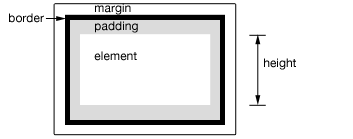
\includegraphics{height1.png}
New in version 1.2: 该方法也可以用来得到 windw 和 document 的高度
\begin{Verbatim}[commandchars=\\\{\}]
\PYG{n+nx}{KISSY}\PYG{p}{.}\PYG{n+nx}{use}\PYG{p}{(}\PYG{l+s+s2}{"node"}\PYG{p}{,}\PYG{k+kd}{function}\PYG{p}{(}\PYG{n+nx}{S}\PYG{p}{,}\PYG{n+nx}{Node}\PYG{p}{)}\PYG{p}{\PYGZob{}}
    \PYG{n+nx}{Node}\PYG{p}{.}\PYG{n+nx}{all}\PYG{p}{(}\PYG{n+nb}{window}\PYG{p}{)}\PYG{p}{.}\PYG{n+nx}{height}\PYG{p}{(}\PYG{p}{)}\PYG{p}{;} \PYG{c+c1}{// 得到浏览器可以区域的高度,相当于 DOM.viewportHeight()}
    \PYG{n+nx}{Node}\PYG{p}{.}\PYG{n+nx}{all}\PYG{p}{(}\PYG{n+nb}{document}\PYG{p}{)}\PYG{p}{.}\PYG{n+nx}{height}\PYG{p}{(}\PYG{p}{)}\PYG{p}{;} \PYG{c+c1}{//得到 html 文档的高度,相当于 DOM.docHeight()}
\PYG{p}{\PYGZcb{}}\PYG{p}{)}\PYG{p}{;}
\end{Verbatim}


\subparagraph{例子}
\label{api/core/node/height:id2}
得到各种各样的高度,黄色高亮区域代表 iframe 体。

\begin{Verbatim}[commandchars=\\\{\}]
\PYG{c+cp}{\textless{}!DOCTYPE html\textgreater{}}
\PYG{n+nt}{\textless{}html}\PYG{n+nt}{\textgreater{}}
\PYG{n+nt}{\textless{}head}\PYG{n+nt}{\textgreater{}}
  \PYG{n+nt}{\textless{}style}\PYG{n+nt}{\textgreater{}}
  \PYG{n+nt}{body} \PYG{p}{\PYGZob{}} \PYG{k}{background}\PYG{o}{:}\PYG{n+nb}{yellow}\PYG{p}{;} \PYG{p}{\PYGZcb{}}
  \PYG{n+nt}{button} \PYG{p}{\PYGZob{}} \PYG{k}{font-size}\PYG{o}{:}\PYG{l+m}{12px}\PYG{p}{;} \PYG{k}{margin}\PYG{o}{:}\PYG{l+m}{2px}\PYG{p}{;} \PYG{p}{\PYGZcb{}}
  \PYG{n+nt}{p} \PYG{p}{\PYGZob{}} \PYG{k}{width}\PYG{o}{:}\PYG{l+m}{150px}\PYG{p}{;} \PYG{k}{border}\PYG{o}{:}\PYG{l+m}{1px} \PYG{n+nb}{red} \PYG{k}{solid}\PYG{p}{;} \PYG{p}{\PYGZcb{}}
  \PYG{n+nt}{div} \PYG{p}{\PYGZob{}} \PYG{k}{color}\PYG{o}{:}\PYG{n+nb}{red}\PYG{p}{;} \PYG{k}{font-weight}\PYG{o}{:}\PYG{k}{bold}\PYG{p}{;} \PYG{p}{\PYGZcb{}}
  \PYG{n+nt}{\textless{}/style\textgreater{}}
  \PYG{n+nt}{\textless{}script}\PYG{n+nt}{\textgreater{}}
    \PYG{k}{if}\PYG{p}{(}\PYG{n+nx}{location}\PYG{p}{.}\PYG{n+nx}{host}\PYG{o}{==}\PYG{l+s+s2}{"localhost"}\PYG{p}{)}\PYG{p}{\PYGZob{}}
        \PYG{n+nb}{document}\PYG{p}{.}\PYG{n+nx}{writeln}\PYG{p}{(}\PYG{l+s+s1}{'\textless{}script src="http://localhost/kissy\PYGZus{}git/kissy/build/kissy.js"'}\PYG{o}{+}\PYG{l+s+s1}{'\textgreater{}'}\PYG{o}{+}\PYG{l+s+s1}{'\textless{}'}\PYG{o}{+}\PYG{l+s+s1}{'/'}\PYG{o}{+}\PYG{l+s+s1}{'script\textgreater{}'}\PYG{p}{)}\PYG{p}{;}
    \PYG{p}{\PYGZcb{}}\PYG{k}{else}\PYG{p}{\PYGZob{}}
        \PYG{n+nb}{document}\PYG{p}{.}\PYG{n+nx}{writeln}\PYG{p}{(}\PYG{l+s+s1}{'\textless{}script src="http://yiminghe.github.com/kissy/build/kissy.js"'}\PYG{o}{+}\PYG{l+s+s1}{'\textgreater{}'}\PYG{o}{+}\PYG{l+s+s1}{'\textless{}'}\PYG{o}{+}\PYG{l+s+s1}{'/'}\PYG{o}{+}\PYG{l+s+s1}{'script\textgreater{}'}\PYG{p}{)}\PYG{p}{;}
    \PYG{p}{\PYGZcb{}}
   \PYG{n+nt}{\textless{}/script\textgreater{}}
\PYG{n+nt}{\textless{}/head\textgreater{}}
\PYG{n+nt}{\textless{}body}\PYG{n+nt}{\textgreater{}}
  \PYG{n+nt}{\textless{}button} \PYG{n+na}{id=}\PYG{l+s}{"getp"}\PYG{n+nt}{\textgreater{}}Get Paragraph Height\PYG{n+nt}{\textless{}/button\textgreater{}}
  \PYG{n+nt}{\textless{}button} \PYG{n+na}{id=}\PYG{l+s}{"getd"}\PYG{n+nt}{\textgreater{}}Get Document Height\PYG{n+nt}{\textless{}/button\textgreater{}}
  \PYG{n+nt}{\textless{}button} \PYG{n+na}{id=}\PYG{l+s}{"getw"}\PYG{n+nt}{\textgreater{}}Get Window Height\PYG{n+nt}{\textless{}/button\textgreater{}}

  \PYG{n+nt}{\textless{}div}\PYG{n+nt}{\textgreater{}}\PYG{n+ni}{\&nbsp;}\PYG{n+nt}{\textless{}/div\textgreater{}}
  \PYG{n+nt}{\textless{}p}\PYG{n+nt}{\textgreater{}}
    Sample paragraph to test height
  \PYG{n+nt}{\textless{}/p\textgreater{}}
\PYG{n+nt}{\textless{}script}\PYG{n+nt}{\textgreater{}}
    \PYG{n+nx}{KISSY}\PYG{p}{.}\PYG{n+nx}{use}\PYG{p}{(}\PYG{l+s+s2}{"node"}\PYG{p}{,}\PYG{k+kd}{function}\PYG{p}{(}\PYG{n+nx}{S}\PYG{p}{,}\PYG{n+nx}{Node}\PYG{p}{)}\PYG{p}{\PYGZob{}}
        \PYG{k+kd}{var} \PYG{n+nx}{\$}\PYG{o}{=}\PYG{n+nx}{Node}\PYG{p}{.}\PYG{n+nx}{all}\PYG{p}{;}
        \PYG{k+kd}{function} \PYG{n+nx}{showHeight}\PYG{p}{(}\PYG{n+nx}{ele}\PYG{p}{,} \PYG{n+nx}{h}\PYG{p}{)} \PYG{p}{\PYGZob{}}
          \PYG{n+nx}{\$}\PYG{p}{(}\PYG{l+s+s2}{"div"}\PYG{p}{)}\PYG{p}{.}\PYG{n+nx}{text}\PYG{p}{(}\PYG{l+s+s2}{"The height for the "} \PYG{o}{+} \PYG{n+nx}{ele} \PYG{o}{+}
                        \PYG{l+s+s2}{" is "} \PYG{o}{+} \PYG{n+nx}{h} \PYG{o}{+} \PYG{l+s+s2}{"px."}\PYG{p}{)}\PYG{p}{;}
        \PYG{p}{\PYGZcb{}}
        \PYG{n+nx}{\$}\PYG{p}{(}\PYG{l+s+s2}{"\#getp"}\PYG{p}{)}\PYG{p}{.}\PYG{n+nx}{on}\PYG{p}{(}\PYG{l+s+s2}{"click"}\PYG{p}{,}\PYG{k+kd}{function} \PYG{p}{(}\PYG{p}{)} \PYG{p}{\PYGZob{}}
          \PYG{n+nx}{showHeight}\PYG{p}{(}\PYG{l+s+s2}{"paragraph"}\PYG{p}{,} \PYG{n+nx}{\$}\PYG{p}{(}\PYG{l+s+s2}{"p"}\PYG{p}{)}\PYG{p}{.}\PYG{n+nx}{height}\PYG{p}{(}\PYG{p}{)}\PYG{p}{)}\PYG{p}{;}
        \PYG{p}{\PYGZcb{}}\PYG{p}{)}\PYG{p}{;}
        \PYG{n+nx}{\$}\PYG{p}{(}\PYG{l+s+s2}{"\#getd"}\PYG{p}{)}\PYG{p}{.}\PYG{n+nx}{on}\PYG{p}{(}\PYG{l+s+s2}{"click"}\PYG{p}{,}\PYG{k+kd}{function} \PYG{p}{(}\PYG{p}{)} \PYG{p}{\PYGZob{}}
          \PYG{n+nx}{showHeight}\PYG{p}{(}\PYG{l+s+s2}{"document"}\PYG{p}{,} \PYG{n+nx}{\$}\PYG{p}{(}\PYG{n+nb}{document}\PYG{p}{)}\PYG{p}{.}\PYG{n+nx}{height}\PYG{p}{(}\PYG{p}{)}\PYG{p}{)}\PYG{p}{;}
        \PYG{p}{\PYGZcb{}}\PYG{p}{)}\PYG{p}{;}
        \PYG{n+nx}{\$}\PYG{p}{(}\PYG{l+s+s2}{"\#getw"}\PYG{p}{)}\PYG{p}{.}\PYG{n+nx}{on}\PYG{p}{(}\PYG{l+s+s2}{"click"}\PYG{p}{,}\PYG{k+kd}{function} \PYG{p}{(}\PYG{p}{)} \PYG{p}{\PYGZob{}}
          \PYG{n+nx}{showHeight}\PYG{p}{(}\PYG{l+s+s2}{"window"}\PYG{p}{,} \PYG{n+nx}{\$}\PYG{p}{(}\PYG{n+nb}{window}\PYG{p}{)}\PYG{p}{.}\PYG{n+nx}{height}\PYG{p}{(}\PYG{p}{)}\PYG{p}{)}\PYG{p}{;}
        \PYG{p}{\PYGZcb{}}\PYG{p}{)}\PYG{p}{;}
    \PYG{p}{\PYGZcb{}}\PYG{p}{)}\PYG{p}{;}
\PYG{n+nt}{\textless{}/script\textgreater{}}

\PYG{n+nt}{\textless{}/body\textgreater{}}
\PYG{n+nt}{\textless{}/html\textgreater{}}
\end{Verbatim}


\subparagraph{效果}
\label{api/core/node/height:id3}

\paragraph{写}
\label{api/core/node/height:id4}
\index{height() (Node.NodeList method)}

\begin{fulllineitems}
\pysiglinewithargsret{\code{NodeList.}\bfcode{height}}{\emph{value}}{}
设置当前列表每个元素的 css height 值。
\begin{quote}\begin{description}
\item[{Parameters}] \leavevmode
\textbf{value} (\emph{number\textbar{}string}) -- 代表像素的整数值,或数字加上其他单位的字符串值.

\end{description}\end{quote}

\end{fulllineitems}


\begin{notice}{note}{Note:}
在现代浏览器中,css height 属性不包括 padding , border 或者 margin.
\end{notice}


\subparagraph{例子}
\label{api/core/node/height:id5}
\begin{Verbatim}[commandchars=\\\{\}]
\PYG{c+cp}{\textless{}!DOCTYPE html\textgreater{}}
\PYG{n+nt}{\textless{}html}\PYG{n+nt}{\textgreater{}}
\PYG{n+nt}{\textless{}head}\PYG{n+nt}{\textgreater{}}
  \PYG{n+nt}{\textless{}style}\PYG{n+nt}{\textgreater{}}\PYG{n+nt}{div} \PYG{p}{\PYGZob{}} \PYG{k}{width}\PYG{o}{:}\PYG{l+m}{50px}\PYG{p}{;} \PYG{k}{height}\PYG{o}{:}\PYG{l+m}{70px}\PYG{p}{;} \PYG{k}{float}\PYG{o}{:}\PYG{k}{left}\PYG{p}{;} \PYG{k}{margin}\PYG{o}{:}\PYG{l+m}{5px}\PYG{p}{;}
        \PYG{k}{background}\PYG{o}{:}\PYG{k}{rgb}\PYG{p}{(}\PYG{l+m}{255}\PYG{o}{,}\PYG{l+m}{140}\PYG{o}{,}\PYG{l+m}{0}\PYG{p}{);} \PYG{k}{cursor}\PYG{o}{:}\PYG{k}{pointer}\PYG{p}{;} \PYG{p}{\PYGZcb{}}  \PYG{n+nt}{\textless{}/style\textgreater{}}
  \PYG{n+nt}{\textless{}script}\PYG{n+nt}{\textgreater{}}
    \PYG{k}{if}\PYG{p}{(}\PYG{n+nx}{location}\PYG{p}{.}\PYG{n+nx}{host}\PYG{o}{==}\PYG{l+s+s2}{"localhost"}\PYG{p}{)}\PYG{p}{\PYGZob{}}
        \PYG{n+nb}{document}\PYG{p}{.}\PYG{n+nx}{writeln}\PYG{p}{(}\PYG{l+s+s1}{'\textless{}script src="http://localhost/kissy\PYGZus{}git/kissy/build/kissy.js"'}\PYG{o}{+}\PYG{l+s+s1}{'\textgreater{}'}\PYG{o}{+}\PYG{l+s+s1}{'\textless{}'}\PYG{o}{+}\PYG{l+s+s1}{'/'}\PYG{o}{+}\PYG{l+s+s1}{'script\textgreater{}'}\PYG{p}{)}\PYG{p}{;}
    \PYG{p}{\PYGZcb{}}\PYG{k}{else}\PYG{p}{\PYGZob{}}
        \PYG{n+nb}{document}\PYG{p}{.}\PYG{n+nx}{writeln}\PYG{p}{(}\PYG{l+s+s1}{'\textless{}script src="http://yiminghe.github.com/kissy/build/kissy.js"'}\PYG{o}{+}\PYG{l+s+s1}{'\textgreater{}'}\PYG{o}{+}\PYG{l+s+s1}{'\textless{}'}\PYG{o}{+}\PYG{l+s+s1}{'/'}\PYG{o}{+}\PYG{l+s+s1}{'script\textgreater{}'}\PYG{p}{)}\PYG{p}{;}
    \PYG{p}{\PYGZcb{}}
   \PYG{n+nt}{\textless{}/script\textgreater{}}
\PYG{n+nt}{\textless{}/head\textgreater{}}
\PYG{n+nt}{\textless{}body}\PYG{n+nt}{\textgreater{}}
  \PYG{n+nt}{\textless{}div}\PYG{n+nt}{\textgreater{}}\PYG{n+nt}{\textless{}/div\textgreater{}}
  \PYG{n+nt}{\textless{}div}\PYG{n+nt}{\textgreater{}}\PYG{n+nt}{\textless{}/div\textgreater{}}

  \PYG{n+nt}{\textless{}div}\PYG{n+nt}{\textgreater{}}\PYG{n+nt}{\textless{}/div\textgreater{}}
  \PYG{n+nt}{\textless{}div}\PYG{n+nt}{\textgreater{}}\PYG{n+nt}{\textless{}/div\textgreater{}}
  \PYG{n+nt}{\textless{}div}\PYG{n+nt}{\textgreater{}}\PYG{n+nt}{\textless{}/div\textgreater{}}
\PYG{n+nt}{\textless{}script}\PYG{n+nt}{\textgreater{}}
    \PYG{n+nx}{KISSY}\PYG{p}{.}\PYG{n+nx}{use}\PYG{p}{(}\PYG{l+s+s2}{"node"}\PYG{p}{,}\PYG{k+kd}{function}\PYG{p}{(}\PYG{n+nx}{S}\PYG{p}{,}\PYG{n+nx}{Node}\PYG{p}{)}\PYG{p}{\PYGZob{}}
        \PYG{k+kd}{var} \PYG{n+nx}{\$}\PYG{o}{=}\PYG{n+nx}{Node}\PYG{p}{.}\PYG{n+nx}{all}\PYG{p}{;}
        \PYG{k+kd}{function} \PYG{n+nx}{handle}\PYG{p}{(}\PYG{p}{)}\PYG{p}{\PYGZob{}}
            \PYG{n+nx}{\$}\PYG{p}{(}\PYG{k}{this}\PYG{p}{)}\PYG{p}{.}\PYG{n+nx}{detach}\PYG{p}{(}\PYG{p}{)}\PYG{p}{;}
            \PYG{n+nx}{\$}\PYG{p}{(}\PYG{k}{this}\PYG{p}{)}\PYG{p}{.}\PYG{n+nx}{height}\PYG{p}{(}\PYG{l+m+mi}{30}\PYG{p}{)}
                 \PYG{p}{.}\PYG{n+nx}{css}\PYG{p}{(}\PYG{p}{\PYGZob{}}\PYG{n+nx}{cursor}\PYG{o}{:}\PYG{l+s+s2}{"auto"}\PYG{p}{,} \PYG{n+nx}{backgroundColor}\PYG{o}{:}\PYG{l+s+s2}{"green"}\PYG{p}{\PYGZcb{}}\PYG{p}{)}\PYG{p}{;}
        \PYG{p}{\PYGZcb{}}
        \PYG{n+nx}{\$}\PYG{p}{(}\PYG{l+s+s2}{"div"}\PYG{p}{)}\PYG{p}{.}\PYG{n+nx}{on}\PYG{p}{(}\PYG{l+s+s1}{'click'}\PYG{p}{,} \PYG{n+nx}{handle}\PYG{p}{)}\PYG{p}{;}
    \PYG{p}{\PYGZcb{}}\PYG{p}{)}\PYG{p}{;}
\PYG{n+nt}{\textless{}/script\textgreater{}}

\PYG{n+nt}{\textless{}/body\textgreater{}}
\PYG{n+nt}{\textless{}/html\textgreater{}}
\end{Verbatim}


\subparagraph{效果}
\label{api/core/node/height:id6}

\subsubsection{width()}
\label{api/core/node/width:width}\label{api/core/node/width::doc}

\paragraph{读}
\label{api/core/node/width:id1}
\index{width() (Node.NodeList method)}

\begin{fulllineitems}
\phantomsection\label{api/core/node/width:Node.NodeList.width}\pysiglinewithargsret{\code{NodeList.}\bfcode{width}}{}{}
得到当前节点列表第一个节点的计算宽度
\begin{quote}\begin{description}
\item[{Return type}] \leavevmode
number

\end{description}\end{quote}

\end{fulllineitems}


和 \code{css('width')} 的区别在于该函数返回不带单位的纯数值,而前者则返回带单位的原始值(例如 \code{400px} ).
当需要数值计算时,推荐该方法。
New in version 1.2: 该方法也可以用来得到 windw 和 document 的宽度
\begin{Verbatim}[commandchars=\\\{\}]
\PYG{n+nx}{KISSY}\PYG{p}{.}\PYG{n+nx}{use}\PYG{p}{(}\PYG{l+s+s2}{"node"}\PYG{p}{,}\PYG{k+kd}{function}\PYG{p}{(}\PYG{n+nx}{S}\PYG{p}{,}\PYG{n+nx}{Node}\PYG{p}{)}\PYG{p}{\PYGZob{}}
    \PYG{n+nx}{Node}\PYG{p}{.}\PYG{n+nx}{all}\PYG{p}{(}\PYG{n+nb}{window}\PYG{p}{)}\PYG{p}{.}\PYG{n+nx}{width}\PYG{p}{(}\PYG{p}{)}\PYG{p}{;} \PYG{c+c1}{// 得到浏览器可以区域的高度,相当于 DOM.viewportWidth()}
    \PYG{n+nx}{Node}\PYG{p}{.}\PYG{n+nx}{all}\PYG{p}{(}\PYG{n+nb}{document}\PYG{p}{)}\PYG{p}{.}\PYG{n+nx}{width}\PYG{p}{(}\PYG{p}{)}\PYG{p}{;} \PYG{c+c1}{//得到 html 文档的高度,相当于 DOM.docWidth()}
\PYG{p}{\PYGZcb{}}\PYG{p}{)}\PYG{p}{;}
\end{Verbatim}


\paragraph{写}
\label{api/core/node/width:id2}
\index{width() (Node.NodeList method)}

\begin{fulllineitems}
\pysiglinewithargsret{\code{NodeList.}\bfcode{width}}{\emph{value}}{}
设置当前列表每个元素的 css width 值。
\begin{quote}\begin{description}
\item[{Parameters}] \leavevmode
\textbf{value} (\emph{number\textbar{}string}) -- 代表像素的整数值,或数字加上其他单位的字符串值.

\end{description}\end{quote}

\end{fulllineitems}


\begin{notice}{note}{Note:}
在现代浏览器中,css width 属性不包括 padding , border 或者 margin.
\end{notice}

例子可参考 {\hyperref[api/core/node/height:Node.NodeList.height]{\code{NodeList.height()}}}


\subsubsection{addStyleSheet()}
\label{api/core/node/addStyleSheet:addstylesheet}\label{api/core/node/addStyleSheet::doc}
\index{addStyleSheet() (Node.NodeList method)}

\begin{fulllineitems}
\phantomsection\label{api/core/node/addStyleSheet:Node.NodeList.addStyleSheet}\pysiglinewithargsret{\code{NodeList.}\bfcode{addStyleSheet}}{\emph{cssText}\optional{, \emph{id}}}{}~New in version 1.2: 将 cssText 字符串作为内联样式添加到文档中。\begin{quote}\begin{description}
\item[{Parameters}] \leavevmode\begin{itemize}
\item {}
\textbf{cssText} (\emph{string}) -- 样式内容

\item {}
\textbf{id} (\emph{string}) -- 内联样式所在 style 节点的 id

\end{itemize}

\item[{Return type}] \leavevmode
NodeList

\item[{Returns}] \leavevmode
当前对象

\end{description}\end{quote}

\end{fulllineitems}


\begin{notice}{note}{Note:}
该方法只可以在 window 和 document 上调用,例如:

\begin{Verbatim}[commandchars=\\\{\}]
\PYG{n+nx}{KISSY}\PYG{p}{.}\PYG{n+nx}{use}\PYG{p}{(}\PYG{l+s+s2}{"node"}\PYG{p}{,}\PYG{k+kd}{function}\PYG{p}{(}\PYG{n+nx}{S}\PYG{p}{,}\PYG{n+nx}{Node}\PYG{p}{)}\PYG{p}{\PYGZob{}}
    \PYG{k+kd}{var} \PYG{n+nx}{\$}\PYG{o}{=}\PYG{n+nx}{Node}\PYG{p}{.}\PYG{n+nx}{all}\PYG{p}{;}
    \PYG{n+nx}{\$}\PYG{p}{(}\PYG{n+nb}{window}\PYG{p}{)}\PYG{p}{.}\PYG{n+nx}{addStyleSheet}\PYG{p}{(}\PYG{l+s+s2}{"p \PYGZob{}color:red;\PYGZcb{}"}\PYG{p}{)}\PYG{p}{;} \PYG{c+c1}{// 段落颜色全部显示为红色}
    \PYG{c+c1}{// 或}
    \PYG{n+nx}{\$}\PYG{p}{(}\PYG{n+nb}{document}\PYG{p}{)}\PYG{p}{.}\PYG{n+nx}{addStyleSheet}\PYG{p}{(}\PYG{l+s+s2}{"p \PYGZob{}color:red;\PYGZcb{}"}\PYG{p}{,}\PYG{l+s+s2}{"addCss"}\PYG{p}{)}\PYG{p}{;}
\PYG{p}{\PYGZcb{}}\PYG{p}{)}\PYG{p}{;}
\end{Verbatim}
\end{notice}


\subsubsection{append()}
\label{api/core/node/append::doc}\label{api/core/node/append:append}
\index{append() (Node.NodeList method)}

\begin{fulllineitems}
\phantomsection\label{api/core/node/append:Node.NodeList.append}\pysiglinewithargsret{\code{NodeList.}\bfcode{append}}{\emph{content}}{}
将参数内容插入到当前节点列表中的每个元素的末尾.
\begin{quote}\begin{description}
\item[{Parameters}] \leavevmode
\textbf{content} (\emph{HTMLELement\textbar{}string\textbar{}NodeList}) -- 将要插入的内容

\item[{Return type}] \leavevmode
NodeList

\end{description}\end{quote}

\end{fulllineitems}


该方法插入指定内容到当前节点列表的最后一个元素后面(如果要插入到第一个元素前面,请用 {\hyperref[api/core/node/prepend:Node.NodeList.prepend]{\code{prepend()}}} ).

该方法和 {\hyperref[api/core/node/appendTo:Node.NodeList.appendTo]{\code{appendTo()}}} 功能一样。最大的区别在于语法不同以及参数意义不同。当使用 \code{append} 方法时,当前节点列表为参数内容的插入容器。
而对于 \code{appendTo}  当前节点列表则为要插入的元素,而参数则为目标容器.

例如如下 HTML:

\begin{Verbatim}[commandchars=\\\{\}]
\PYG{n+nt}{\textless{}h2}\PYG{n+nt}{\textgreater{}}Greetings\PYG{n+nt}{\textless{}/h2\textgreater{}}
\PYG{n+nt}{\textless{}div} \PYG{n+na}{class=}\PYG{l+s}{"container"}\PYG{n+nt}{\textgreater{}}
  \PYG{n+nt}{\textless{}div} \PYG{n+na}{class=}\PYG{l+s}{"inner"}\PYG{n+nt}{\textgreater{}}Hello\PYG{n+nt}{\textless{}/div\textgreater{}}
  \PYG{n+nt}{\textless{}div} \PYG{n+na}{class=}\PYG{l+s}{"inner"}\PYG{n+nt}{\textgreater{}}Goodbye\PYG{n+nt}{\textless{}/div\textgreater{}}
\PYG{n+nt}{\textless{}/div\textgreater{}}
\end{Verbatim}

你可以创建 NodeList 并把它立即插入到指定容器中:

\begin{Verbatim}[commandchars=\\\{\}]
\PYG{n+nx}{KISSY}\PYG{p}{.}\PYG{n+nx}{use}\PYG{p}{(}\PYG{l+s+s2}{"node"}\PYG{p}{,}\PYG{k+kd}{function}\PYG{p}{(}\PYG{n+nx}{S}\PYG{p}{,}\PYG{n+nx}{NodeList}\PYG{p}{)}\PYG{p}{\PYGZob{}}
    \PYG{n+nx}{NodeList}\PYG{p}{.}\PYG{n+nx}{all}\PYG{p}{(}\PYG{l+s+s1}{'.inner'}\PYG{p}{)}\PYG{p}{.}\PYG{n+nx}{append}\PYG{p}{(}\PYG{l+s+s1}{'\textless{}p\textgreater{}Test\textless{}/p\textgreater{}'}\PYG{p}{)}\PYG{p}{;}
\PYG{p}{\PYGZcb{}}\PYG{p}{)}\PYG{p}{;}
\end{Verbatim}

内层的每个 div 元素都得到了新内容

\begin{Verbatim}[commandchars=\\\{\}]
\PYG{n+nt}{\textless{}h2}\PYG{n+nt}{\textgreater{}}Greetings\PYG{n+nt}{\textless{}/h2\textgreater{}}
\PYG{n+nt}{\textless{}div} \PYG{n+na}{class=}\PYG{l+s}{"container"}\PYG{n+nt}{\textgreater{}}
  \PYG{n+nt}{\textless{}div} \PYG{n+na}{class=}\PYG{l+s}{"inner"}\PYG{n+nt}{\textgreater{}}
    Hello
    \PYG{n+nt}{\textless{}p}\PYG{n+nt}{\textgreater{}}Test\PYG{n+nt}{\textless{}/p\textgreater{}}
  \PYG{n+nt}{\textless{}/div\textgreater{}}
  \PYG{n+nt}{\textless{}div} \PYG{n+na}{class=}\PYG{l+s}{"inner"}\PYG{n+nt}{\textgreater{}}
    Goodbye
    \PYG{n+nt}{\textless{}p}\PYG{n+nt}{\textgreater{}}Test\PYG{n+nt}{\textless{}/p\textgreater{}}
  \PYG{n+nt}{\textless{}/div\textgreater{}}
\PYG{n+nt}{\textless{}/div\textgreater{}}
\end{Verbatim}

你可以把页面上已有的元素 \code{prepend} 到另外一个:

\begin{Verbatim}[commandchars=\\\{\}]
\PYG{n+nx}{KISSY}\PYG{p}{.}\PYG{n+nx}{use}\PYG{p}{(}\PYG{l+s+s2}{"node"}\PYG{p}{,}\PYG{k+kd}{function}\PYG{p}{(}\PYG{n+nx}{S}\PYG{p}{,}\PYG{n+nx}{NodeList}\PYG{p}{)}\PYG{p}{\PYGZob{}}
    \PYG{n+nx}{NodeList}\PYG{p}{.}\PYG{n+nx}{all}\PYG{p}{(}\PYG{l+s+s1}{'.container'}\PYG{p}{)}\PYG{p}{.}\PYG{n+nx}{append}\PYG{p}{(}\PYG{n+nx}{\$}\PYG{p}{(}\PYG{l+s+s1}{'h2'}\PYG{p}{)}\PYG{p}{)}\PYG{p}{;}
\PYG{p}{\PYGZcb{}}\PYG{p}{)}\PYG{p}{;}
\end{Verbatim}

如果当前节点列表只包括一个节点,那么他将会被移到目标容器中(而不是克隆):

\begin{Verbatim}[commandchars=\\\{\}]
\PYG{n+nt}{\textless{}div} \PYG{n+na}{class=}\PYG{l+s}{"container"}\PYG{n+nt}{\textgreater{}}
  \PYG{n+nt}{\textless{}div} \PYG{n+na}{class=}\PYG{l+s}{"inner"}\PYG{n+nt}{\textgreater{}}Hello\PYG{n+nt}{\textless{}/div\textgreater{}}
  \PYG{n+nt}{\textless{}div} \PYG{n+na}{class=}\PYG{l+s}{"inner"}\PYG{n+nt}{\textgreater{}}Goodbye\PYG{n+nt}{\textless{}/div\textgreater{}}
  \PYG{n+nt}{\textless{}h2}\PYG{n+nt}{\textgreater{}}Greetings\PYG{n+nt}{\textless{}/h2\textgreater{}}
\PYG{n+nt}{\textless{}/div\textgreater{}}
\end{Verbatim}

但是如果当前节点列表包括多余一个节点,则除了第一个节点外,其他节点都添加的是参数节点的克隆节点。


\paragraph{例子}
\label{api/core/node/append:id1}
在所有段落中添加一些 html 字符串

\begin{Verbatim}[commandchars=\\\{\}]
    \PYG{c+cp}{\textless{}!DOCTYPE html\textgreater{}}
    \PYG{n+nt}{\textless{}html}\PYG{n+nt}{\textgreater{}}
    \PYG{n+nt}{\textless{}head}\PYG{n+nt}{\textgreater{}}
      \PYG{n+nt}{\textless{}style}\PYG{n+nt}{\textgreater{}}
      \PYG{n+nt}{p} \PYG{p}{\PYGZob{}} \PYG{k}{background}\PYG{o}{:}\PYG{n+nb}{yellow}\PYG{p}{;} \PYG{p}{\PYGZcb{}}
    \PYG{n+nt}{\textless{}/style\textgreater{}}
     \PYG{n+nt}{\textless{}script}\PYG{n+nt}{\textgreater{}}
    \PYG{k}{if}\PYG{p}{(}\PYG{n+nx}{location}\PYG{p}{.}\PYG{n+nx}{host}\PYG{o}{==}\PYG{l+s+s2}{"localhost"}\PYG{p}{)}\PYG{p}{\PYGZob{}}
        \PYG{n+nb}{document}\PYG{p}{.}\PYG{n+nx}{writeln}\PYG{p}{(}\PYG{l+s+s1}{'\textless{}script src="http://localhost/kissy\PYGZus{}git/kissy/build/kissy.js"'}\PYG{o}{+}\PYG{l+s+s1}{'\textgreater{}'}\PYG{o}{+}\PYG{l+s+s1}{'\textless{}'}\PYG{o}{+}\PYG{l+s+s1}{'/'}\PYG{o}{+}\PYG{l+s+s1}{'script\textgreater{}'}\PYG{p}{)}\PYG{p}{;}
    \PYG{p}{\PYGZcb{}}\PYG{k}{else}\PYG{p}{\PYGZob{}}
        \PYG{n+nb}{document}\PYG{p}{.}\PYG{n+nx}{writeln}\PYG{p}{(}\PYG{l+s+s1}{'\textless{}script src="http://yiminghe.github.com/kissy/build/kissy.js"'}\PYG{o}{+}\PYG{l+s+s1}{'\textgreater{}'}\PYG{o}{+}\PYG{l+s+s1}{'\textless{}'}\PYG{o}{+}\PYG{l+s+s1}{'/'}\PYG{o}{+}\PYG{l+s+s1}{'script\textgreater{}'}\PYG{p}{)}\PYG{p}{;}
    \PYG{p}{\PYGZcb{}}
   \PYG{n+nt}{\textless{}/script\textgreater{}}
    \PYG{n+nt}{\textless{}/head\textgreater{}}
    \PYG{n+nt}{\textless{}body}\PYG{n+nt}{\textgreater{}}
      \PYG{n+nt}{\textless{}p}\PYG{n+nt}{\textgreater{}} is I would like to say \PYG{n+nt}{\textless{}/p\textgreater{}}
    \PYG{n+nt}{\textless{}script}\PYG{n+nt}{\textgreater{}}
        \PYG{n+nx}{KISSY}\PYG{p}{.}\PYG{n+nx}{use}\PYG{p}{(}\PYG{l+s+s2}{"node"}\PYG{p}{,}\PYG{k+kd}{function}\PYG{p}{(}\PYG{n+nx}{S}\PYG{p}{,}\PYG{n+nx}{NodeList}\PYG{p}{)}\PYG{p}{\PYGZob{}}
            \PYG{n+nx}{NodeList}\PYG{p}{.}\PYG{n+nx}{all}\PYG{p}{(}\PYG{l+s+s2}{"p"}\PYG{p}{)}\PYG{p}{.}\PYG{n+nx}{append}\PYG{p}{(}\PYG{l+s+s2}{"\textless{}strong\textgreater{}Hello\textless{}/strong\textgreater{}"}\PYG{p}{)}\PYG{p}{;}
        \PYG{p}{\PYGZcb{}}\PYG{p}{)}\PYG{p}{;}
    \PYG{n+nt}{\textless{}/script\textgreater{}}

    \PYG{n+nt}{\textless{}/body\textgreater{}}
    \PYG{n+nt}{\textless{}/html\textgreater{}}
\end{Verbatim}

Demo

给所有段落添加一个文本节点

\begin{Verbatim}[commandchars=\\\{\}]
    \PYG{c+cp}{\textless{}!DOCTYPE html\textgreater{}}
    \PYG{n+nt}{\textless{}html}\PYG{n+nt}{\textgreater{}}
    \PYG{n+nt}{\textless{}head}\PYG{n+nt}{\textgreater{}}
      \PYG{n+nt}{\textless{}style}\PYG{n+nt}{\textgreater{}}
      \PYG{n+nt}{p} \PYG{p}{\PYGZob{}} \PYG{k}{background}\PYG{o}{:}\PYG{n+nb}{yellow}\PYG{p}{;} \PYG{p}{\PYGZcb{}}
    \PYG{n+nt}{\textless{}/style\textgreater{}}
     \PYG{n+nt}{\textless{}script}\PYG{n+nt}{\textgreater{}}
    \PYG{k}{if}\PYG{p}{(}\PYG{n+nx}{location}\PYG{p}{.}\PYG{n+nx}{host}\PYG{o}{==}\PYG{l+s+s2}{"localhost"}\PYG{p}{)}\PYG{p}{\PYGZob{}}
        \PYG{n+nb}{document}\PYG{p}{.}\PYG{n+nx}{writeln}\PYG{p}{(}\PYG{l+s+s1}{'\textless{}script src="http://localhost/kissy\PYGZus{}git/kissy/build/kissy.js"'}\PYG{o}{+}\PYG{l+s+s1}{'\textgreater{}'}\PYG{o}{+}\PYG{l+s+s1}{'\textless{}'}\PYG{o}{+}\PYG{l+s+s1}{'/'}\PYG{o}{+}\PYG{l+s+s1}{'script\textgreater{}'}\PYG{p}{)}\PYG{p}{;}
    \PYG{p}{\PYGZcb{}}\PYG{k}{else}\PYG{p}{\PYGZob{}}
        \PYG{n+nb}{document}\PYG{p}{.}\PYG{n+nx}{writeln}\PYG{p}{(}\PYG{l+s+s1}{'\textless{}script src="http://yiminghe.github.com/kissy/build/kissy.js"'}\PYG{o}{+}\PYG{l+s+s1}{'\textgreater{}'}\PYG{o}{+}\PYG{l+s+s1}{'\textless{}'}\PYG{o}{+}\PYG{l+s+s1}{'/'}\PYG{o}{+}\PYG{l+s+s1}{'script\textgreater{}'}\PYG{p}{)}\PYG{p}{;}
    \PYG{p}{\PYGZcb{}}
   \PYG{n+nt}{\textless{}/script\textgreater{}}
    \PYG{n+nt}{\textless{}/head\textgreater{}}
    \PYG{n+nt}{\textless{}body}\PYG{n+nt}{\textgreater{}}
      \PYG{n+nt}{\textless{}p}\PYG{n+nt}{\textgreater{}}I would like to say: \PYG{n+nt}{\textless{}/p\textgreater{}}
      \PYG{n+nt}{\textless{}p}\PYG{n+nt}{\textgreater{}}I also would like to say: \PYG{n+nt}{\textless{}/p\textgreater{}}
    \PYG{n+nt}{\textless{}script}\PYG{n+nt}{\textgreater{}}
        \PYG{n+nx}{KISSY}\PYG{p}{.}\PYG{n+nx}{use}\PYG{p}{(}\PYG{l+s+s2}{"node"}\PYG{p}{,}\PYG{k+kd}{function}\PYG{p}{(}\PYG{n+nx}{S}\PYG{p}{,}\PYG{n+nx}{NodeList}\PYG{p}{)}\PYG{p}{\PYGZob{}}
            \PYG{n+nx}{NodeList}\PYG{p}{.}\PYG{n+nx}{all}\PYG{p}{(}\PYG{l+s+s2}{"p"}\PYG{p}{)}\PYG{p}{.}\PYG{n+nx}{append}\PYG{p}{(}\PYG{n+nb}{document}\PYG{p}{.}\PYG{n+nx}{createTextNode}\PYG{p}{(}\PYG{l+s+s2}{"Hello"}\PYG{p}{)}\PYG{p}{)}\PYG{p}{;}
        \PYG{p}{\PYGZcb{}}\PYG{p}{)}\PYG{p}{;}
    \PYG{n+nt}{\textless{}/script\textgreater{}}

    \PYG{n+nt}{\textless{}/body\textgreater{}}
    \PYG{n+nt}{\textless{}/html\textgreater{}}
\end{Verbatim}

Demo

给所有段落添加一个 \code{NodeList}  对象

\begin{Verbatim}[commandchars=\\\{\}]
    \PYG{c+cp}{\textless{}!DOCTYPE html\textgreater{}}
    \PYG{n+nt}{\textless{}html}\PYG{n+nt}{\textgreater{}}
    \PYG{n+nt}{\textless{}head}\PYG{n+nt}{\textgreater{}}
      \PYG{n+nt}{\textless{}style}\PYG{n+nt}{\textgreater{}}
      \PYG{n+nt}{p} \PYG{p}{\PYGZob{}} \PYG{k}{background}\PYG{o}{:}\PYG{n+nb}{yellow}\PYG{p}{;} \PYG{p}{\PYGZcb{}}
    \PYG{n+nt}{\textless{}/style\textgreater{}}
     \PYG{n+nt}{\textless{}script}\PYG{n+nt}{\textgreater{}}
    \PYG{k}{if}\PYG{p}{(}\PYG{n+nx}{location}\PYG{p}{.}\PYG{n+nx}{host}\PYG{o}{==}\PYG{l+s+s2}{"localhost"}\PYG{p}{)}\PYG{p}{\PYGZob{}}
        \PYG{n+nb}{document}\PYG{p}{.}\PYG{n+nx}{writeln}\PYG{p}{(}\PYG{l+s+s1}{'\textless{}script src="http://localhost/kissy\PYGZus{}git/kissy/build/kissy.js"'}\PYG{o}{+}\PYG{l+s+s1}{'\textgreater{}'}\PYG{o}{+}\PYG{l+s+s1}{'\textless{}'}\PYG{o}{+}\PYG{l+s+s1}{'/'}\PYG{o}{+}\PYG{l+s+s1}{'script\textgreater{}'}\PYG{p}{)}\PYG{p}{;}
    \PYG{p}{\PYGZcb{}}\PYG{k}{else}\PYG{p}{\PYGZob{}}
        \PYG{n+nb}{document}\PYG{p}{.}\PYG{n+nx}{writeln}\PYG{p}{(}\PYG{l+s+s1}{'\textless{}script src="http://yiminghe.github.com/kissy/build/kissy.js"'}\PYG{o}{+}\PYG{l+s+s1}{'\textgreater{}'}\PYG{o}{+}\PYG{l+s+s1}{'\textless{}'}\PYG{o}{+}\PYG{l+s+s1}{'/'}\PYG{o}{+}\PYG{l+s+s1}{'script\textgreater{}'}\PYG{p}{)}\PYG{p}{;}
    \PYG{p}{\PYGZcb{}}
   \PYG{n+nt}{\textless{}/script\textgreater{}}
    \PYG{n+nt}{\textless{}/head\textgreater{}}
    \PYG{n+nt}{\textless{}body}\PYG{n+nt}{\textgreater{}}
        \PYG{n+nt}{\textless{}strong}\PYG{n+nt}{\textgreater{}}Hello world!!!\PYG{n+nt}{\textless{}/strong\textgreater{}}\PYG{n+nt}{\textless{}p}\PYG{n+nt}{\textgreater{}}I would like to say: \PYG{n+nt}{\textless{}/p\textgreater{}}

    \PYG{n+nt}{\textless{}script}\PYG{n+nt}{\textgreater{}}
        \PYG{n+nx}{KISSY}\PYG{p}{.}\PYG{n+nx}{use}\PYG{p}{(}\PYG{l+s+s2}{"node"}\PYG{p}{,}\PYG{k+kd}{function}\PYG{p}{(}\PYG{n+nx}{S}\PYG{p}{,}\PYG{n+nx}{NodeList}\PYG{p}{)}\PYG{p}{\PYGZob{}}
            \PYG{n+nx}{NodeList}\PYG{p}{.}\PYG{n+nx}{all}\PYG{p}{(}\PYG{l+s+s2}{"p"}\PYG{p}{)}\PYG{p}{.}\PYG{n+nx}{append}\PYG{p}{(}\PYG{n+nx}{NodeList}\PYG{p}{.}\PYG{n+nx}{all}\PYG{p}{(}\PYG{l+s+s2}{"strong"}\PYG{p}{)}\PYG{p}{)}\PYG{p}{;}
        \PYG{p}{\PYGZcb{}}\PYG{p}{)}\PYG{p}{;}
    \PYG{n+nt}{\textless{}/script\textgreater{}}

    \PYG{n+nt}{\textless{}/body\textgreater{}}
    \PYG{n+nt}{\textless{}/html\textgreater{}}
\end{Verbatim}

Demo


\subsubsection{appendTo()}
\label{api/core/node/appendTo:appendto}\label{api/core/node/appendTo::doc}
\index{appendTo() (Node.NodeList method)}

\begin{fulllineitems}
\phantomsection\label{api/core/node/appendTo:Node.NodeList.appendTo}\pysiglinewithargsret{\code{NodeList.}\bfcode{appendTo}}{\emph{containers}}{}
将当前节点列表中的每个元素插入到容器列表的每个元素的最后一个子节点后面.
\begin{quote}\begin{description}
\item[{Parameters}] \leavevmode
\textbf{content} (\emph{HTMLELement\textbar{}string\textbar{}NodeList}) --
将要插入的内容
\begin{itemize}
\item {}
HTMLELement\textbar{}NodeList: 已有或新创建的节点

\item {}
string: 选择器字符串,查找已有的容器节点

\end{itemize}


\item[{Return type}] \leavevmode
NodeList

\end{description}\end{quote}

\end{fulllineitems}


\code{appendTo} 和 {\hyperref[api/core/node/append:Node.NodeList.append]{\code{append()}}} 功能一样,只不过参数意义不同.

考虑下面 html 字符串:

\begin{Verbatim}[commandchars=\\\{\}]
\PYG{n+nt}{\textless{}h2}\PYG{n+nt}{\textgreater{}}Greetings\PYG{n+nt}{\textless{}/h2\textgreater{}}
\PYG{n+nt}{\textless{}div} \PYG{n+na}{class=}\PYG{l+s}{"container"}\PYG{n+nt}{\textgreater{}}
  \PYG{n+nt}{\textless{}div} \PYG{n+na}{class=}\PYG{l+s}{"inner"}\PYG{n+nt}{\textgreater{}}Hello\PYG{n+nt}{\textless{}/div\textgreater{}}
  \PYG{n+nt}{\textless{}div} \PYG{n+na}{class=}\PYG{l+s}{"inner"}\PYG{n+nt}{\textgreater{}}Goodbye\PYG{n+nt}{\textless{}/div\textgreater{}}
\PYG{n+nt}{\textless{}/div\textgreater{}}
\end{Verbatim}

我们可以创建元素后立即插入到多个已有元素:

\begin{Verbatim}[commandchars=\\\{\}]
\PYG{n+nx}{NodeList}\PYG{p}{.}\PYG{n+nx}{all}\PYG{p}{(}\PYG{l+s+s1}{'\textless{}p\textgreater{}Test\textless{}/p\textgreater{}'}\PYG{p}{)}\PYG{p}{.}\PYG{n+nx}{appendTo}\PYG{p}{(}\PYG{l+s+s1}{'.inner'}\PYG{p}{)}\PYG{p}{;}
\end{Verbatim}

每个内层 div 元素都得到了新内容

\begin{Verbatim}[commandchars=\\\{\}]
\PYG{n+nt}{\textless{}h2}\PYG{n+nt}{\textgreater{}}Greetings\PYG{n+nt}{\textless{}/h2\textgreater{}}
\PYG{n+nt}{\textless{}div} \PYG{n+na}{class=}\PYG{l+s}{"container"}\PYG{n+nt}{\textgreater{}}
  \PYG{n+nt}{\textless{}div} \PYG{n+na}{class=}\PYG{l+s}{"inner"}\PYG{n+nt}{\textgreater{}}
    Hello
    \PYG{n+nt}{\textless{}p}\PYG{n+nt}{\textgreater{}}Test\PYG{n+nt}{\textless{}/p\textgreater{}}
  \PYG{n+nt}{\textless{}/div\textgreater{}}
  \PYG{n+nt}{\textless{}div} \PYG{n+na}{class=}\PYG{l+s}{"inner"}\PYG{n+nt}{\textgreater{}}
    Goodbye
    \PYG{n+nt}{\textless{}p}\PYG{n+nt}{\textgreater{}}Test\PYG{n+nt}{\textless{}/p\textgreater{}}
  \PYG{n+nt}{\textless{}/div\textgreater{}}
\PYG{n+nt}{\textless{}/div\textgreater{}}
\end{Verbatim}

我们也可以把一个已有元素插入到另一个

\begin{Verbatim}[commandchars=\\\{\}]
\PYG{n+nx}{NodeList}\PYG{p}{.}\PYG{n+nx}{all}\PYG{p}{(}\PYG{l+s+s1}{'h2'}\PYG{p}{)}\PYG{p}{.}\PYG{n+nx}{appendTo}\PYG{p}{(}\PYG{n+nx}{NodeList}\PYG{p}{.}\PYG{n+nx}{all}\PYG{p}{(}\PYG{l+s+s1}{'.container'}\PYG{p}{)}\PYG{p}{)}\PYG{p}{;}
\end{Verbatim}

如果容器列表只有一个节点,那么当前节点列表会被移动到容器内(不是克隆):

\begin{Verbatim}[commandchars=\\\{\}]
\PYG{n+nt}{\textless{}div} \PYG{n+na}{class=}\PYG{l+s}{"container"}\PYG{n+nt}{\textgreater{}}
  \PYG{n+nt}{\textless{}div} \PYG{n+na}{class=}\PYG{l+s}{"inner"}\PYG{n+nt}{\textgreater{}}Hello\PYG{n+nt}{\textless{}/div\textgreater{}}
  \PYG{n+nt}{\textless{}div} \PYG{n+na}{class=}\PYG{l+s}{"inner"}\PYG{n+nt}{\textgreater{}}Goodbye\PYG{n+nt}{\textless{}/div\textgreater{}}
  \PYG{n+nt}{\textless{}h2}\PYG{n+nt}{\textgreater{}}Greetings\PYG{n+nt}{\textless{}/h2\textgreater{}}
\PYG{n+nt}{\textless{}/div\textgreater{}}
\end{Verbatim}

不过如果有多个目标容器,那么除了第一个目标容器,当前节点列表的复制节点会被插入到其他目标容器


\paragraph{例子}
\label{api/core/node/appendTo:id1}
把多个 span 插入到已有元素

\begin{Verbatim}[commandchars=\\\{\}]
\PYG{c+cp}{\textless{}!DOCTYPE html\textgreater{}}
\PYG{n+nt}{\textless{}html}\PYG{n+nt}{\textgreater{}}
\PYG{n+nt}{\textless{}head}\PYG{n+nt}{\textgreater{}}
  \PYG{n+nt}{\textless{}style}\PYG{n+nt}{\textgreater{}}\PYG{n+nt}{div} \PYG{p}{\PYGZob{}} \PYG{k}{background}\PYG{o}{:}\PYG{n+nb}{yellow}\PYG{p}{;} \PYG{p}{\PYGZcb{}}\PYG{n+nt}{\textless{}/style\textgreater{}}
  \PYG{n+nt}{\textless{}script}\PYG{n+nt}{\textgreater{}}
    \PYG{k}{if}\PYG{p}{(}\PYG{n+nx}{location}\PYG{p}{.}\PYG{n+nx}{host}\PYG{o}{==}\PYG{l+s+s2}{"localhost"}\PYG{p}{)}\PYG{p}{\PYGZob{}}
        \PYG{n+nb}{document}\PYG{p}{.}\PYG{n+nx}{writeln}\PYG{p}{(}\PYG{l+s+s1}{'\textless{}script src="http://localhost/kissy\PYGZus{}git/kissy/build/kissy.js"'}\PYG{o}{+}\PYG{l+s+s1}{'\textgreater{}'}\PYG{o}{+}\PYG{l+s+s1}{'\textless{}'}\PYG{o}{+}\PYG{l+s+s1}{'/'}\PYG{o}{+}\PYG{l+s+s1}{'script\textgreater{}'}\PYG{p}{)}\PYG{p}{;}
    \PYG{p}{\PYGZcb{}}\PYG{k}{else}\PYG{p}{\PYGZob{}}
        \PYG{n+nb}{document}\PYG{p}{.}\PYG{n+nx}{writeln}\PYG{p}{(}\PYG{l+s+s1}{'\textless{}script src="http://yiminghe.github.com/kissy/build/kissy.js"'}\PYG{o}{+}\PYG{l+s+s1}{'\textgreater{}'}\PYG{o}{+}\PYG{l+s+s1}{'\textless{}'}\PYG{o}{+}\PYG{l+s+s1}{'/'}\PYG{o}{+}\PYG{l+s+s1}{'script\textgreater{}'}\PYG{p}{)}\PYG{p}{;}
    \PYG{p}{\PYGZcb{}}
   \PYG{n+nt}{\textless{}/script\textgreater{}}
\PYG{n+nt}{\textless{}/head\textgreater{}}
\PYG{n+nt}{\textless{}body}\PYG{n+nt}{\textgreater{}}
    \PYG{n+nt}{\textless{}div} \PYG{n+na}{id=}\PYG{l+s}{"foo"}\PYG{n+nt}{\textgreater{}}FOO! is \PYG{n+nt}{\textless{}/div\textgreater{}}

    \PYG{n+nt}{\textless{}span}\PYG{n+nt}{\textgreater{}}I have something to say... \PYG{n+nt}{\textless{}/span\textgreater{}}

    \PYG{n+nt}{\textless{}span}\PYG{n+nt}{\textgreater{}} once more : \PYG{n+nt}{\textless{}/span\textgreater{}}

    \PYG{n+nt}{\textless{}script}\PYG{n+nt}{\textgreater{}}
        \PYG{n+nx}{KISSY}\PYG{p}{.}\PYG{n+nx}{use}\PYG{p}{(}\PYG{l+s+s2}{"node"}\PYG{p}{,}\PYG{k+kd}{function}\PYG{p}{(}\PYG{n+nx}{S}\PYG{p}{,}\PYG{n+nx}{NodeList}\PYG{p}{)}\PYG{p}{\PYGZob{}}
            \PYG{n+nx}{NodeList}\PYG{p}{.}\PYG{n+nx}{all}\PYG{p}{(}\PYG{l+s+s2}{"span"}\PYG{p}{)}\PYG{p}{.}\PYG{n+nx}{appendTo}\PYG{p}{(}\PYG{n+nx}{NodeList}\PYG{p}{.}\PYG{n+nx}{all}\PYG{p}{(}\PYG{l+s+s2}{"\#foo"}\PYG{p}{)}\PYG{p}{)}\PYG{p}{;}
        \PYG{p}{\PYGZcb{}}\PYG{p}{)}\PYG{p}{;}
    \PYG{n+nt}{\textless{}/script\textgreater{}}
\PYG{n+nt}{\textless{}/body\textgreater{}}
\PYG{n+nt}{\textless{}/html\textgreater{}}
\end{Verbatim}

Demo


\subsubsection{prepend()}
\label{api/core/node/prepend::doc}\label{api/core/node/prepend:prepend}
\index{prepend() (Node.NodeList method)}

\begin{fulllineitems}
\phantomsection\label{api/core/node/prepend:Node.NodeList.prepend}\pysiglinewithargsret{\code{NodeList.}\bfcode{prepend}}{\emph{content}}{}
将参数内容插入到当前节点列表中的每个元素的开头.
\begin{quote}\begin{description}
\item[{Parameters}] \leavevmode
\textbf{content} (\emph{HTMLELement\textbar{}string\textbar{}NodeList}) -- 将要插入的内容

\item[{Return type}] \leavevmode
NodeList

\end{description}\end{quote}

\end{fulllineitems}


该方法插入指定内容到当前节点列表的第一个元素前面(如果要插入到最后一个元素后面,请用 {\hyperref[api/core/node/append:Node.NodeList.append]{\code{append()}}} ).

该方法和 {\hyperref[api/core/node/prependTo:Node.NodeList.prependTo]{\code{prependTo()}}} 功能一样。最大的区别在于语法不同以及参数意义不同。当使用 \code{prepend} 方法时,当前节点列表为参数内容的插入容器。
而对于 \code{prependTo}  当前节点列表则为要插入的元素,而参数则为目标容器.

例如如下 HTML:

\begin{Verbatim}[commandchars=\\\{\}]
\PYG{n+nt}{\textless{}h2}\PYG{n+nt}{\textgreater{}}Greetings\PYG{n+nt}{\textless{}/h2\textgreater{}}
\PYG{n+nt}{\textless{}div} \PYG{n+na}{class=}\PYG{l+s}{"container"}\PYG{n+nt}{\textgreater{}}
  \PYG{n+nt}{\textless{}div} \PYG{n+na}{class=}\PYG{l+s}{"inner"}\PYG{n+nt}{\textgreater{}}Hello\PYG{n+nt}{\textless{}/div\textgreater{}}
  \PYG{n+nt}{\textless{}div} \PYG{n+na}{class=}\PYG{l+s}{"inner"}\PYG{n+nt}{\textgreater{}}Goodbye\PYG{n+nt}{\textless{}/div\textgreater{}}
\PYG{n+nt}{\textless{}/div\textgreater{}}
\end{Verbatim}

你可以创建 NodeList 并把它立即插入到指定容器中:

\begin{Verbatim}[commandchars=\\\{\}]
\PYG{n+nx}{KISSY}\PYG{p}{.}\PYG{n+nx}{use}\PYG{p}{(}\PYG{l+s+s2}{"node"}\PYG{p}{,}\PYG{k+kd}{function}\PYG{p}{(}\PYG{n+nx}{S}\PYG{p}{,}\PYG{n+nx}{NodeList}\PYG{p}{)}\PYG{p}{\PYGZob{}}
    \PYG{n+nx}{NodeList}\PYG{p}{.}\PYG{n+nx}{all}\PYG{p}{(}\PYG{l+s+s1}{'.inner'}\PYG{p}{)}\PYG{p}{.}\PYG{n+nx}{prepend}\PYG{p}{(}\PYG{l+s+s1}{'\textless{}p\textgreater{}Test\textless{}/p\textgreater{}'}\PYG{p}{)}\PYG{p}{;}
\PYG{p}{\PYGZcb{}}\PYG{p}{)}\PYG{p}{;}
\end{Verbatim}

内层的每个 div 元素都得到了新内容

\begin{Verbatim}[commandchars=\\\{\}]
\PYG{n+nt}{\textless{}h2}\PYG{n+nt}{\textgreater{}}Greetings\PYG{n+nt}{\textless{}/h2\textgreater{}}
\PYG{n+nt}{\textless{}div} \PYG{n+na}{class=}\PYG{l+s}{"container"}\PYG{n+nt}{\textgreater{}}
  \PYG{n+nt}{\textless{}div} \PYG{n+na}{class=}\PYG{l+s}{"inner"}\PYG{n+nt}{\textgreater{}}
    \PYG{n+nt}{\textless{}p}\PYG{n+nt}{\textgreater{}}Test\PYG{n+nt}{\textless{}/p\textgreater{}}
    Hello
  \PYG{n+nt}{\textless{}/div\textgreater{}}
  \PYG{n+nt}{\textless{}div} \PYG{n+na}{class=}\PYG{l+s}{"inner"}\PYG{n+nt}{\textgreater{}}
    \PYG{n+nt}{\textless{}p}\PYG{n+nt}{\textgreater{}}Test\PYG{n+nt}{\textless{}/p\textgreater{}}
    Goodbye
  \PYG{n+nt}{\textless{}/div\textgreater{}}
\PYG{n+nt}{\textless{}/div\textgreater{}}
\end{Verbatim}

你可以把页面上已有的元素 \code{prepend} 到另外一个:

\begin{Verbatim}[commandchars=\\\{\}]
\PYG{n+nx}{KISSY}\PYG{p}{.}\PYG{n+nx}{use}\PYG{p}{(}\PYG{l+s+s2}{"node"}\PYG{p}{,}\PYG{k+kd}{function}\PYG{p}{(}\PYG{n+nx}{S}\PYG{p}{,}\PYG{n+nx}{NodeList}\PYG{p}{)}\PYG{p}{\PYGZob{}}
    \PYG{n+nx}{NodeList}\PYG{p}{.}\PYG{n+nx}{all}\PYG{p}{(}\PYG{l+s+s1}{'.container'}\PYG{p}{)}\PYG{p}{.}\PYG{n+nx}{prepend}\PYG{p}{(}\PYG{n+nx}{\$}\PYG{p}{(}\PYG{l+s+s1}{'h2'}\PYG{p}{)}\PYG{p}{)}\PYG{p}{;}
\PYG{p}{\PYGZcb{}}\PYG{p}{)}\PYG{p}{;}
\end{Verbatim}

如果当前节点列表只包括一个节点,那么他将会被移到目标容器中(而不是克隆):

\begin{Verbatim}[commandchars=\\\{\}]
\PYG{n+nt}{\textless{}div} \PYG{n+na}{class=}\PYG{l+s}{"container"}\PYG{n+nt}{\textgreater{}}
    \PYG{n+nt}{\textless{}h2}\PYG{n+nt}{\textgreater{}}Greetings\PYG{n+nt}{\textless{}/h2\textgreater{}}
    \PYG{n+nt}{\textless{}div} \PYG{n+na}{class=}\PYG{l+s}{"inner"}\PYG{n+nt}{\textgreater{}}Hello\PYG{n+nt}{\textless{}/div\textgreater{}}
    \PYG{n+nt}{\textless{}div} \PYG{n+na}{class=}\PYG{l+s}{"inner"}\PYG{n+nt}{\textgreater{}}Goodbye\PYG{n+nt}{\textless{}/div\textgreater{}}
\PYG{n+nt}{\textless{}/div\textgreater{}}
\end{Verbatim}

但是如果当前节点列表包括多余一个节点,则除了第一个节点外,其他节点都添加的是参数节点的克隆节点。


\paragraph{例子}
\label{api/core/node/prepend:id1}
在所有段落中添加一些 html 字符串

\begin{Verbatim}[commandchars=\\\{\}]
    \PYG{c+cp}{\textless{}!DOCTYPE html\textgreater{}}
    \PYG{n+nt}{\textless{}html}\PYG{n+nt}{\textgreater{}}
    \PYG{n+nt}{\textless{}head}\PYG{n+nt}{\textgreater{}}
      \PYG{n+nt}{\textless{}style}\PYG{n+nt}{\textgreater{}}
      \PYG{n+nt}{p} \PYG{p}{\PYGZob{}} \PYG{k}{background}\PYG{o}{:}\PYG{n+nb}{yellow}\PYG{p}{;} \PYG{p}{\PYGZcb{}}
    \PYG{n+nt}{\textless{}/style\textgreater{}}
     \PYG{n+nt}{\textless{}script}\PYG{n+nt}{\textgreater{}}
    \PYG{k}{if}\PYG{p}{(}\PYG{n+nx}{location}\PYG{p}{.}\PYG{n+nx}{host}\PYG{o}{==}\PYG{l+s+s2}{"localhost"}\PYG{p}{)}\PYG{p}{\PYGZob{}}
        \PYG{n+nb}{document}\PYG{p}{.}\PYG{n+nx}{writeln}\PYG{p}{(}\PYG{l+s+s1}{'\textless{}script src="http://localhost/kissy\PYGZus{}git/kissy/build/kissy.js"'}\PYG{o}{+}\PYG{l+s+s1}{'\textgreater{}'}\PYG{o}{+}\PYG{l+s+s1}{'\textless{}'}\PYG{o}{+}\PYG{l+s+s1}{'/'}\PYG{o}{+}\PYG{l+s+s1}{'script\textgreater{}'}\PYG{p}{)}\PYG{p}{;}
    \PYG{p}{\PYGZcb{}}\PYG{k}{else}\PYG{p}{\PYGZob{}}
        \PYG{n+nb}{document}\PYG{p}{.}\PYG{n+nx}{writeln}\PYG{p}{(}\PYG{l+s+s1}{'\textless{}script src="http://yiminghe.github.com/kissy/build/kissy.js"'}\PYG{o}{+}\PYG{l+s+s1}{'\textgreater{}'}\PYG{o}{+}\PYG{l+s+s1}{'\textless{}'}\PYG{o}{+}\PYG{l+s+s1}{'/'}\PYG{o}{+}\PYG{l+s+s1}{'script\textgreater{}'}\PYG{p}{)}\PYG{p}{;}
    \PYG{p}{\PYGZcb{}}
   \PYG{n+nt}{\textless{}/script\textgreater{}}
    \PYG{n+nt}{\textless{}/head\textgreater{}}
    \PYG{n+nt}{\textless{}body}\PYG{n+nt}{\textgreater{}}
      \PYG{n+nt}{\textless{}p}\PYG{n+nt}{\textgreater{}}I would like to say: \PYG{n+nt}{\textless{}/p\textgreater{}}
    \PYG{n+nt}{\textless{}script}\PYG{n+nt}{\textgreater{}}
        \PYG{n+nx}{KISSY}\PYG{p}{.}\PYG{n+nx}{use}\PYG{p}{(}\PYG{l+s+s2}{"node"}\PYG{p}{,}\PYG{k+kd}{function}\PYG{p}{(}\PYG{n+nx}{S}\PYG{p}{,}\PYG{n+nx}{NodeList}\PYG{p}{)}\PYG{p}{\PYGZob{}}
            \PYG{n+nx}{NodeList}\PYG{p}{.}\PYG{n+nx}{all}\PYG{p}{(}\PYG{l+s+s2}{"p"}\PYG{p}{)}\PYG{p}{.}\PYG{n+nx}{prepend}\PYG{p}{(}\PYG{l+s+s2}{"\textless{}strong\textgreater{}Hello\textless{}/strong\textgreater{}"}\PYG{p}{)}\PYG{p}{;}
        \PYG{p}{\PYGZcb{}}\PYG{p}{)}\PYG{p}{;}
    \PYG{n+nt}{\textless{}/script\textgreater{}}

    \PYG{n+nt}{\textless{}/body\textgreater{}}
    \PYG{n+nt}{\textless{}/html\textgreater{}}
\end{Verbatim}

Demo

给所有段落添加一个文本节点

\begin{Verbatim}[commandchars=\\\{\}]
    \PYG{c+cp}{\textless{}!DOCTYPE html\textgreater{}}
    \PYG{n+nt}{\textless{}html}\PYG{n+nt}{\textgreater{}}
    \PYG{n+nt}{\textless{}head}\PYG{n+nt}{\textgreater{}}
      \PYG{n+nt}{\textless{}style}\PYG{n+nt}{\textgreater{}}
      \PYG{n+nt}{p} \PYG{p}{\PYGZob{}} \PYG{k}{background}\PYG{o}{:}\PYG{n+nb}{yellow}\PYG{p}{;} \PYG{p}{\PYGZcb{}}
    \PYG{n+nt}{\textless{}/style\textgreater{}}
     \PYG{n+nt}{\textless{}script}\PYG{n+nt}{\textgreater{}}
    \PYG{k}{if}\PYG{p}{(}\PYG{n+nx}{location}\PYG{p}{.}\PYG{n+nx}{host}\PYG{o}{==}\PYG{l+s+s2}{"localhost"}\PYG{p}{)}\PYG{p}{\PYGZob{}}
        \PYG{n+nb}{document}\PYG{p}{.}\PYG{n+nx}{writeln}\PYG{p}{(}\PYG{l+s+s1}{'\textless{}script src="http://localhost/kissy\PYGZus{}git/kissy/build/kissy.js"'}\PYG{o}{+}\PYG{l+s+s1}{'\textgreater{}'}\PYG{o}{+}\PYG{l+s+s1}{'\textless{}'}\PYG{o}{+}\PYG{l+s+s1}{'/'}\PYG{o}{+}\PYG{l+s+s1}{'script\textgreater{}'}\PYG{p}{)}\PYG{p}{;}
    \PYG{p}{\PYGZcb{}}\PYG{k}{else}\PYG{p}{\PYGZob{}}
        \PYG{n+nb}{document}\PYG{p}{.}\PYG{n+nx}{writeln}\PYG{p}{(}\PYG{l+s+s1}{'\textless{}script src="http://yiminghe.github.com/kissy/build/kissy.js"'}\PYG{o}{+}\PYG{l+s+s1}{'\textgreater{}'}\PYG{o}{+}\PYG{l+s+s1}{'\textless{}'}\PYG{o}{+}\PYG{l+s+s1}{'/'}\PYG{o}{+}\PYG{l+s+s1}{'script\textgreater{}'}\PYG{p}{)}\PYG{p}{;}
    \PYG{p}{\PYGZcb{}}
   \PYG{n+nt}{\textless{}/script\textgreater{}}
    \PYG{n+nt}{\textless{}/head\textgreater{}}
    \PYG{n+nt}{\textless{}body}\PYG{n+nt}{\textgreater{}}
      \PYG{n+nt}{\textless{}p}\PYG{n+nt}{\textgreater{}} is I would like to say \PYG{n+nt}{\textless{}/p\textgreater{}}
      \PYG{n+nt}{\textless{}p}\PYG{n+nt}{\textgreater{}} is also I would like to say\PYG{n+nt}{\textless{}/p\textgreater{}}
    \PYG{n+nt}{\textless{}script}\PYG{n+nt}{\textgreater{}}
        \PYG{n+nx}{KISSY}\PYG{p}{.}\PYG{n+nx}{use}\PYG{p}{(}\PYG{l+s+s2}{"node"}\PYG{p}{,}\PYG{k+kd}{function}\PYG{p}{(}\PYG{n+nx}{S}\PYG{p}{,}\PYG{n+nx}{NodeList}\PYG{p}{)}\PYG{p}{\PYGZob{}}
            \PYG{n+nx}{NodeList}\PYG{p}{.}\PYG{n+nx}{all}\PYG{p}{(}\PYG{l+s+s2}{"p"}\PYG{p}{)}\PYG{p}{.}\PYG{n+nx}{prepend}\PYG{p}{(}\PYG{n+nb}{document}\PYG{p}{.}\PYG{n+nx}{createTextNode}\PYG{p}{(}\PYG{l+s+s2}{"Hello"}\PYG{p}{)}\PYG{p}{)}\PYG{p}{;}
        \PYG{p}{\PYGZcb{}}\PYG{p}{)}\PYG{p}{;}
    \PYG{n+nt}{\textless{}/script\textgreater{}}

    \PYG{n+nt}{\textless{}/body\textgreater{}}
    \PYG{n+nt}{\textless{}/html\textgreater{}}
\end{Verbatim}

Demo

给所有段落添加一个 \code{NodeList}  对象

\begin{Verbatim}[commandchars=\\\{\}]
    \PYG{c+cp}{\textless{}!DOCTYPE html\textgreater{}}
    \PYG{n+nt}{\textless{}html}\PYG{n+nt}{\textgreater{}}
    \PYG{n+nt}{\textless{}head}\PYG{n+nt}{\textgreater{}}
      \PYG{n+nt}{\textless{}style}\PYG{n+nt}{\textgreater{}}
      \PYG{n+nt}{p} \PYG{p}{\PYGZob{}} \PYG{k}{background}\PYG{o}{:}\PYG{n+nb}{yellow}\PYG{p}{;} \PYG{p}{\PYGZcb{}}
    \PYG{n+nt}{\textless{}/style\textgreater{}}
     \PYG{n+nt}{\textless{}script}\PYG{n+nt}{\textgreater{}}
    \PYG{k}{if}\PYG{p}{(}\PYG{n+nx}{location}\PYG{p}{.}\PYG{n+nx}{host}\PYG{o}{==}\PYG{l+s+s2}{"localhost"}\PYG{p}{)}\PYG{p}{\PYGZob{}}
        \PYG{n+nb}{document}\PYG{p}{.}\PYG{n+nx}{writeln}\PYG{p}{(}\PYG{l+s+s1}{'\textless{}script src="http://localhost/kissy\PYGZus{}git/kissy/build/kissy.js"'}\PYG{o}{+}\PYG{l+s+s1}{'\textgreater{}'}\PYG{o}{+}\PYG{l+s+s1}{'\textless{}'}\PYG{o}{+}\PYG{l+s+s1}{'/'}\PYG{o}{+}\PYG{l+s+s1}{'script\textgreater{}'}\PYG{p}{)}\PYG{p}{;}
    \PYG{p}{\PYGZcb{}}\PYG{k}{else}\PYG{p}{\PYGZob{}}
        \PYG{n+nb}{document}\PYG{p}{.}\PYG{n+nx}{writeln}\PYG{p}{(}\PYG{l+s+s1}{'\textless{}script src="http://yiminghe.github.com/kissy/build/kissy.js"'}\PYG{o}{+}\PYG{l+s+s1}{'\textgreater{}'}\PYG{o}{+}\PYG{l+s+s1}{'\textless{}'}\PYG{o}{+}\PYG{l+s+s1}{'/'}\PYG{o}{+}\PYG{l+s+s1}{'script\textgreater{}'}\PYG{p}{)}\PYG{p}{;}
    \PYG{p}{\PYGZcb{}}
   \PYG{n+nt}{\textless{}/script\textgreater{}}
    \PYG{n+nt}{\textless{}/head\textgreater{}}
    \PYG{n+nt}{\textless{}body}\PYG{n+nt}{\textgreater{}}
       \PYG{n+nt}{\textless{}p}\PYG{n+nt}{\textgreater{}} is I would like to say \PYG{n+nt}{\textless{}/p\textgreater{}} \PYG{n+nt}{\textless{}strong}\PYG{n+nt}{\textgreater{}}Hello world!!!\PYG{n+nt}{\textless{}/strong\textgreater{}}

    \PYG{n+nt}{\textless{}script}\PYG{n+nt}{\textgreater{}}
        \PYG{n+nx}{KISSY}\PYG{p}{.}\PYG{n+nx}{use}\PYG{p}{(}\PYG{l+s+s2}{"node"}\PYG{p}{,}\PYG{k+kd}{function}\PYG{p}{(}\PYG{n+nx}{S}\PYG{p}{,}\PYG{n+nx}{NodeList}\PYG{p}{)}\PYG{p}{\PYGZob{}}
            \PYG{n+nx}{NodeList}\PYG{p}{.}\PYG{n+nx}{all}\PYG{p}{(}\PYG{l+s+s2}{"p"}\PYG{p}{)}\PYG{p}{.}\PYG{n+nx}{prepend}\PYG{p}{(}\PYG{n+nx}{NodeList}\PYG{p}{.}\PYG{n+nx}{all}\PYG{p}{(}\PYG{l+s+s2}{"strong"}\PYG{p}{)}\PYG{p}{)}\PYG{p}{;}
        \PYG{p}{\PYGZcb{}}\PYG{p}{)}\PYG{p}{;}
    \PYG{n+nt}{\textless{}/script\textgreater{}}

    \PYG{n+nt}{\textless{}/body\textgreater{}}
    \PYG{n+nt}{\textless{}/html\textgreater{}}
\end{Verbatim}

Demo


\subsubsection{prependTo()}
\label{api/core/node/prependTo:prependto}\label{api/core/node/prependTo::doc}
\index{prependTo() (Node.NodeList method)}

\begin{fulllineitems}
\phantomsection\label{api/core/node/prependTo:Node.NodeList.prependTo}\pysiglinewithargsret{\code{NodeList.}\bfcode{prependTo}}{\emph{containers}}{}
将当前节点列表中的每个元素插入到容器列表的每个元素的开头.
\begin{quote}\begin{description}
\item[{Parameters}] \leavevmode
\textbf{content} (\emph{HTMLELement\textbar{}string\textbar{}NodeList}) --
将要插入的内容
\begin{itemize}
\item {}
HTMLELement\textbar{}NodeList: 已有或新创建的节点

\item {}
string: 选择器字符串,查找已有的容器节点

\end{itemize}


\item[{Return type}] \leavevmode
NodeList

\end{description}\end{quote}

\end{fulllineitems}


\code{prependTo} 和 {\hyperref[api/core/node/prepend:Node.NodeList.prepend]{\code{prepend()}}} 功能一样,只不过参数意义不同.

考虑下面 html 字符串:

\begin{Verbatim}[commandchars=\\\{\}]
\PYG{n+nt}{\textless{}h2}\PYG{n+nt}{\textgreater{}}Greetings\PYG{n+nt}{\textless{}/h2\textgreater{}}
\PYG{n+nt}{\textless{}div} \PYG{n+na}{class=}\PYG{l+s}{"container"}\PYG{n+nt}{\textgreater{}}
  \PYG{n+nt}{\textless{}div} \PYG{n+na}{class=}\PYG{l+s}{"inner"}\PYG{n+nt}{\textgreater{}}Hello\PYG{n+nt}{\textless{}/div\textgreater{}}
  \PYG{n+nt}{\textless{}div} \PYG{n+na}{class=}\PYG{l+s}{"inner"}\PYG{n+nt}{\textgreater{}}Goodbye\PYG{n+nt}{\textless{}/div\textgreater{}}
\PYG{n+nt}{\textless{}/div\textgreater{}}
\end{Verbatim}

我们可以创建元素后立即插入到多个已有元素:

\begin{Verbatim}[commandchars=\\\{\}]
\PYG{n+nx}{NodeList}\PYG{p}{.}\PYG{n+nx}{all}\PYG{p}{(}\PYG{l+s+s1}{'\textless{}p\textgreater{}Test\textless{}/p\textgreater{}'}\PYG{p}{)}\PYG{p}{.}\PYG{n+nx}{prependTo}\PYG{p}{(}\PYG{l+s+s1}{'.inner'}\PYG{p}{)}\PYG{p}{;}
\end{Verbatim}

每个内层 div 元素都得到了新内容

\begin{Verbatim}[commandchars=\\\{\}]
\PYG{n+nt}{\textless{}h2}\PYG{n+nt}{\textgreater{}}Greetings\PYG{n+nt}{\textless{}/h2\textgreater{}}
\PYG{n+nt}{\textless{}div} \PYG{n+na}{class=}\PYG{l+s}{"container"}\PYG{n+nt}{\textgreater{}}
  \PYG{n+nt}{\textless{}div} \PYG{n+na}{class=}\PYG{l+s}{"inner"}\PYG{n+nt}{\textgreater{}}
    \PYG{n+nt}{\textless{}p}\PYG{n+nt}{\textgreater{}}Test\PYG{n+nt}{\textless{}/p\textgreater{}}
    Hello
  \PYG{n+nt}{\textless{}/div\textgreater{}}
  \PYG{n+nt}{\textless{}div} \PYG{n+na}{class=}\PYG{l+s}{"inner"}\PYG{n+nt}{\textgreater{}}
    \PYG{n+nt}{\textless{}p}\PYG{n+nt}{\textgreater{}}Test\PYG{n+nt}{\textless{}/p\textgreater{}}
    Goodbye
  \PYG{n+nt}{\textless{}/div\textgreater{}}
\PYG{n+nt}{\textless{}/div\textgreater{}}
\end{Verbatim}

我们也可以把一个已有元素插入到另一个

\begin{Verbatim}[commandchars=\\\{\}]
\PYG{n+nx}{NodeList}\PYG{p}{.}\PYG{n+nx}{all}\PYG{p}{(}\PYG{l+s+s1}{'h2'}\PYG{p}{)}\PYG{p}{.}\PYG{n+nx}{prependTo}\PYG{p}{(}\PYG{n+nx}{NodeList}\PYG{p}{.}\PYG{n+nx}{all}\PYG{p}{(}\PYG{l+s+s1}{'.container'}\PYG{p}{)}\PYG{p}{)}\PYG{p}{;}
\end{Verbatim}

如果容器列表只有一个节点,那么当前节点列表会被移动到容器内(不是克隆):

\begin{Verbatim}[commandchars=\\\{\}]
\PYG{n+nt}{\textless{}div} \PYG{n+na}{class=}\PYG{l+s}{"container"}\PYG{n+nt}{\textgreater{}}
  \PYG{n+nt}{\textless{}h2}\PYG{n+nt}{\textgreater{}}Greetings\PYG{n+nt}{\textless{}/h2\textgreater{}}
  \PYG{n+nt}{\textless{}div} \PYG{n+na}{class=}\PYG{l+s}{"inner"}\PYG{n+nt}{\textgreater{}}Hello\PYG{n+nt}{\textless{}/div\textgreater{}}
  \PYG{n+nt}{\textless{}div} \PYG{n+na}{class=}\PYG{l+s}{"inner"}\PYG{n+nt}{\textgreater{}}Goodbye\PYG{n+nt}{\textless{}/div\textgreater{}}
\PYG{n+nt}{\textless{}/div\textgreater{}}
\end{Verbatim}

不过如果有多个目标容器,那么除了第一个目标容器,当前节点列表的复制节点会被插入到其他目标容器


\paragraph{例子}
\label{api/core/node/prependTo:id1}
把多个 span 插入到已有元素

\begin{Verbatim}[commandchars=\\\{\}]
\PYG{c+cp}{\textless{}!DOCTYPE html\textgreater{}}
\PYG{n+nt}{\textless{}html}\PYG{n+nt}{\textgreater{}}
\PYG{n+nt}{\textless{}head}\PYG{n+nt}{\textgreater{}}
  \PYG{n+nt}{\textless{}style}\PYG{n+nt}{\textgreater{}}\PYG{n+nt}{div} \PYG{p}{\PYGZob{}} \PYG{k}{background}\PYG{o}{:}\PYG{n+nb}{yellow}\PYG{p}{;} \PYG{p}{\PYGZcb{}}\PYG{n+nt}{\textless{}/style\textgreater{}}
  \PYG{n+nt}{\textless{}script}\PYG{n+nt}{\textgreater{}}
    \PYG{k}{if}\PYG{p}{(}\PYG{n+nx}{location}\PYG{p}{.}\PYG{n+nx}{host}\PYG{o}{==}\PYG{l+s+s2}{"localhost"}\PYG{p}{)}\PYG{p}{\PYGZob{}}
        \PYG{n+nb}{document}\PYG{p}{.}\PYG{n+nx}{writeln}\PYG{p}{(}\PYG{l+s+s1}{'\textless{}script src="http://localhost/kissy\PYGZus{}git/kissy/build/kissy.js"'}\PYG{o}{+}\PYG{l+s+s1}{'\textgreater{}'}\PYG{o}{+}\PYG{l+s+s1}{'\textless{}'}\PYG{o}{+}\PYG{l+s+s1}{'/'}\PYG{o}{+}\PYG{l+s+s1}{'script\textgreater{}'}\PYG{p}{)}\PYG{p}{;}
    \PYG{p}{\PYGZcb{}}\PYG{k}{else}\PYG{p}{\PYGZob{}}
        \PYG{n+nb}{document}\PYG{p}{.}\PYG{n+nx}{writeln}\PYG{p}{(}\PYG{l+s+s1}{'\textless{}script src="http://yiminghe.github.com/kissy/build/kissy.js"'}\PYG{o}{+}\PYG{l+s+s1}{'\textgreater{}'}\PYG{o}{+}\PYG{l+s+s1}{'\textless{}'}\PYG{o}{+}\PYG{l+s+s1}{'/'}\PYG{o}{+}\PYG{l+s+s1}{'script\textgreater{}'}\PYG{p}{)}\PYG{p}{;}
    \PYG{p}{\PYGZcb{}}
   \PYG{n+nt}{\textless{}/script\textgreater{}}
\PYG{n+nt}{\textless{}/head\textgreater{}}
\PYG{n+nt}{\textless{}body}\PYG{n+nt}{\textgreater{}}
    \PYG{n+nt}{\textless{}div} \PYG{n+na}{id=}\PYG{l+s}{"foo"}\PYG{n+nt}{\textgreater{}}FOO!\PYG{n+nt}{\textless{}/div\textgreater{}}

    \PYG{n+nt}{\textless{}span}\PYG{n+nt}{\textgreater{}}I have something to say... \PYG{n+nt}{\textless{}/span\textgreater{}}

    \PYG{n+nt}{\textless{}span}\PYG{n+nt}{\textgreater{}} once more : \PYG{n+nt}{\textless{}/span\textgreater{}}

    \PYG{n+nt}{\textless{}script}\PYG{n+nt}{\textgreater{}}
        \PYG{n+nx}{KISSY}\PYG{p}{.}\PYG{n+nx}{use}\PYG{p}{(}\PYG{l+s+s2}{"node"}\PYG{p}{,}\PYG{k+kd}{function}\PYG{p}{(}\PYG{n+nx}{S}\PYG{p}{,}\PYG{n+nx}{NodeList}\PYG{p}{)}\PYG{p}{\PYGZob{}}
            \PYG{n+nx}{NodeList}\PYG{p}{.}\PYG{n+nx}{all}\PYG{p}{(}\PYG{l+s+s2}{"span"}\PYG{p}{)}\PYG{p}{.}\PYG{n+nx}{prependTo}\PYG{p}{(}\PYG{n+nx}{NodeList}\PYG{p}{.}\PYG{n+nx}{all}\PYG{p}{(}\PYG{l+s+s2}{"\#foo"}\PYG{p}{)}\PYG{p}{)}\PYG{p}{;}
        \PYG{p}{\PYGZcb{}}\PYG{p}{)}\PYG{p}{;}
    \PYG{n+nt}{\textless{}/script\textgreater{}}
\PYG{n+nt}{\textless{}/body\textgreater{}}
\PYG{n+nt}{\textless{}/html\textgreater{}}
\end{Verbatim}

Demo


\subsubsection{insertBefore()}
\label{api/core/node/insertBefore::doc}\label{api/core/node/insertBefore:insertbefore}
\index{insertBefore() (Node.NodeList method)}

\begin{fulllineitems}
\phantomsection\label{api/core/node/insertBefore:Node.NodeList.insertBefore}\pysiglinewithargsret{\code{NodeList.}\bfcode{insertBefore}}{\emph{target}}{}
将当前列表中的每个元素插入到目标元素之前.
\begin{quote}\begin{description}
\item[{Parameters}] \leavevmode
\textbf{target} (\emph{HTMLElement\textbar{}string\textbar{}NodeList}) --
将要插入的元素
\begin{itemize}
\item {}
string : 选择器字符串

\item {}
HTMLElement\textbar{}NodeList : 已有或新建的元素

\end{itemize}


\end{description}\end{quote}

\end{fulllineitems}


\code{before()} 和该方法的功能一样,只不过参数意义不同,该函数表示当前节点列表被插入到参数目标节点之前,
而 \code{before} 则表示参数节点被插入到当前节点之前.

例如:

\begin{Verbatim}[commandchars=\\\{\}]
\PYG{n+nt}{\textless{}div} \PYG{n+na}{class=}\PYG{l+s}{"container"}\PYG{n+nt}{\textgreater{}}
  \PYG{n+nt}{\textless{}h2}\PYG{n+nt}{\textgreater{}}Greetings\PYG{n+nt}{\textless{}/h2\textgreater{}}
  \PYG{n+nt}{\textless{}div} \PYG{n+na}{class=}\PYG{l+s}{"inner"}\PYG{n+nt}{\textgreater{}}Hello\PYG{n+nt}{\textless{}/div\textgreater{}}
  \PYG{n+nt}{\textless{}div} \PYG{n+na}{class=}\PYG{l+s}{"inner"}\PYG{n+nt}{\textgreater{}}Goodbye\PYG{n+nt}{\textless{}/div\textgreater{}}
\PYG{n+nt}{\textless{}/div\textgreater{}}
\end{Verbatim}

我们可以创建节点并立即把它插入到一些元素之前

\begin{Verbatim}[commandchars=\\\{\}]
\PYG{n+nx}{NodeList}\PYG{p}{.}\PYG{n+nx}{all}\PYG{p}{(}\PYG{l+s+s1}{'\textless{}p\textgreater{}Test\textless{}/p\textgreater{}'}\PYG{p}{)}\PYG{p}{.}\PYG{n+nx}{insertBefore}\PYG{p}{(}\PYG{l+s+s1}{'.inner'}\PYG{p}{)}\PYG{p}{;}
\end{Verbatim}

结果为

\begin{Verbatim}[commandchars=\\\{\}]
\PYG{n+nt}{\textless{}div} \PYG{n+na}{class=}\PYG{l+s}{"container"}\PYG{n+nt}{\textgreater{}}
  \PYG{n+nt}{\textless{}h2}\PYG{n+nt}{\textgreater{}}Greetings\PYG{n+nt}{\textless{}/h2\textgreater{}}
  \PYG{n+nt}{\textless{}p}\PYG{n+nt}{\textgreater{}}Test\PYG{n+nt}{\textless{}/p\textgreater{}}
  \PYG{n+nt}{\textless{}div} \PYG{n+na}{class=}\PYG{l+s}{"inner"}\PYG{n+nt}{\textgreater{}}Hello\PYG{n+nt}{\textless{}/div\textgreater{}}
  \PYG{n+nt}{\textless{}p}\PYG{n+nt}{\textgreater{}}Test\PYG{n+nt}{\textless{}/p\textgreater{}}
  \PYG{n+nt}{\textless{}div} \PYG{n+na}{class=}\PYG{l+s}{"inner"}\PYG{n+nt}{\textgreater{}}Goodbye\PYG{n+nt}{\textless{}/div\textgreater{}}
\PYG{n+nt}{\textless{}/div\textgreater{}}
\end{Verbatim}

我们也可以操纵现有元素

\begin{Verbatim}[commandchars=\\\{\}]
\PYG{n+nx}{NodeList}\PYG{p}{.}\PYG{n+nx}{all}\PYG{p}{(}\PYG{l+s+s1}{'h2'}\PYG{p}{)}\PYG{p}{.}\PYG{n+nx}{insertBefore}\PYG{p}{(}\PYG{n+nx}{NodeList}\PYG{p}{.}\PYG{n+nx}{all}\PYG{p}{(}\PYG{l+s+s1}{'.container'}\PYG{p}{)}\PYG{p}{)}\PYG{p}{;}
\end{Verbatim}

如果目标节点只有一个,那么当前节点就会移动到目标节点之前

\begin{Verbatim}[commandchars=\\\{\}]
\PYG{n+nt}{\textless{}h2}\PYG{n+nt}{\textgreater{}}Greetings\PYG{n+nt}{\textless{}/h2\textgreater{}}
\PYG{n+nt}{\textless{}div} \PYG{n+na}{class=}\PYG{l+s}{"container"}\PYG{n+nt}{\textgreater{}}
  \PYG{n+nt}{\textless{}div} \PYG{n+na}{class=}\PYG{l+s}{"inner"}\PYG{n+nt}{\textgreater{}}Hello\PYG{n+nt}{\textless{}/div\textgreater{}}
  \PYG{n+nt}{\textless{}div} \PYG{n+na}{class=}\PYG{l+s}{"inner"}\PYG{n+nt}{\textgreater{}}Goodbye\PYG{n+nt}{\textless{}/div\textgreater{}}
\PYG{n+nt}{\textless{}/div\textgreater{}}
\end{Verbatim}

如果有多个目标节点,那么除了第一个目标节点外,其他目标节点前会被插入当前节点的克隆


\paragraph{例子}
\label{api/core/node/insertBefore:id1}
把段落插入到 div 节点之前

\begin{Verbatim}[commandchars=\\\{\}]
    \PYG{c+cp}{\textless{}!DOCTYPE html\textgreater{}}
    \PYG{n+nt}{\textless{}html}\PYG{n+nt}{\textgreater{}}
    \PYG{n+nt}{\textless{}head}\PYG{n+nt}{\textgreater{}}
      \PYG{n+nt}{\textless{}style}\PYG{n+nt}{\textgreater{}}
      \PYG{n+nt}{p} \PYG{p}{\PYGZob{}} \PYG{k}{background}\PYG{o}{:}\PYG{n+nb}{yellow}\PYG{p}{;} \PYG{p}{\PYGZcb{}}
    \PYG{n+nt}{\textless{}/style\textgreater{}}
     \PYG{n+nt}{\textless{}script}\PYG{n+nt}{\textgreater{}}
    \PYG{k}{if}\PYG{p}{(}\PYG{n+nx}{location}\PYG{p}{.}\PYG{n+nx}{host}\PYG{o}{==}\PYG{l+s+s2}{"localhost"}\PYG{p}{)}\PYG{p}{\PYGZob{}}
        \PYG{n+nb}{document}\PYG{p}{.}\PYG{n+nx}{writeln}\PYG{p}{(}\PYG{l+s+s1}{'\textless{}script src="http://localhost/kissy\PYGZus{}git/kissy/build/kissy.js"'}\PYG{o}{+}\PYG{l+s+s1}{'\textgreater{}'}\PYG{o}{+}\PYG{l+s+s1}{'\textless{}'}\PYG{o}{+}\PYG{l+s+s1}{'/'}\PYG{o}{+}\PYG{l+s+s1}{'script\textgreater{}'}\PYG{p}{)}\PYG{p}{;}
    \PYG{p}{\PYGZcb{}}\PYG{k}{else}\PYG{p}{\PYGZob{}}
        \PYG{n+nb}{document}\PYG{p}{.}\PYG{n+nx}{writeln}\PYG{p}{(}\PYG{l+s+s1}{'\textless{}script src="http://yiminghe.github.com/kissy/build/kissy.js"'}\PYG{o}{+}\PYG{l+s+s1}{'\textgreater{}'}\PYG{o}{+}\PYG{l+s+s1}{'\textless{}'}\PYG{o}{+}\PYG{l+s+s1}{'/'}\PYG{o}{+}\PYG{l+s+s1}{'script\textgreater{}'}\PYG{p}{)}\PYG{p}{;}
    \PYG{p}{\PYGZcb{}}
   \PYG{n+nt}{\textless{}/script\textgreater{}}
    \PYG{n+nt}{\textless{}/head\textgreater{}}
   \PYG{n+nt}{\textless{}body}\PYG{n+nt}{\textgreater{}}
  \PYG{n+nt}{\textless{}div} \PYG{n+na}{id=}\PYG{l+s}{"foo"}\PYG{n+nt}{\textgreater{}}FOO!\PYG{n+nt}{\textless{}/div\textgreater{}}\PYG{n+nt}{\textless{}p}\PYG{n+nt}{\textgreater{}}I would like to say: \PYG{n+nt}{\textless{}/p\textgreater{}}

    \PYG{n+nt}{\textless{}script}\PYG{n+nt}{\textgreater{}}
        \PYG{n+nx}{KISSY}\PYG{p}{.}\PYG{n+nx}{use}\PYG{p}{(}\PYG{l+s+s2}{"node"}\PYG{p}{,}\PYG{k+kd}{function}\PYG{p}{(}\PYG{n+nx}{S}\PYG{p}{,}\PYG{n+nx}{NodeList}\PYG{p}{)}\PYG{p}{\PYGZob{}}
            \PYG{n+nx}{NodeList}\PYG{p}{.}\PYG{n+nx}{all}\PYG{p}{(}\PYG{l+s+s2}{"p"}\PYG{p}{)}\PYG{p}{.}\PYG{n+nx}{insertBefore}\PYG{p}{(}\PYG{l+s+s2}{"\#foo"}\PYG{p}{)}\PYG{p}{;}
        \PYG{p}{\PYGZcb{}}\PYG{p}{)}\PYG{p}{;}
    \PYG{n+nt}{\textless{}/script\textgreater{}}

    \PYG{n+nt}{\textless{}/body\textgreater{}}
    \PYG{n+nt}{\textless{}/html\textgreater{}}
\end{Verbatim}

Demo


\subsubsection{before()}
\label{api/core/node/before::doc}\label{api/core/node/before:before}
\index{before() (Node.NodeList method)}

\begin{fulllineitems}
\phantomsection\label{api/core/node/before:Node.NodeList.before}\pysiglinewithargsret{\code{NodeList.}\bfcode{before}}{\emph{content}}{}~Changed in version 1.2: 将参数内容插入到当前列表中每个元素之前.\begin{quote}\begin{description}
\item[{Parameters}] \leavevmode
\textbf{content} (\emph{HTMLElement\textbar{}string\textbar{}NodeList}) --
将要插入的元素
\begin{itemize}
\item {}
string : html 字符串

\item {}
HTMLElement\textbar{}NodeList : 已有或新建的元素

\end{itemize}


\end{description}\end{quote}

\end{fulllineitems}


\code{insertBefore()} 和该方法的功能一样,只不过参数意义不同,{}`{}`insertBefore{}`{}` 表示当前节点列表被插入到参数目标节点之前,
而该方法则表示参数节点被插入到当前节点之前.

例如:

\begin{Verbatim}[commandchars=\\\{\}]
\PYG{n+nt}{\textless{}div} \PYG{n+na}{class=}\PYG{l+s}{"container"}\PYG{n+nt}{\textgreater{}}
  \PYG{n+nt}{\textless{}h2}\PYG{n+nt}{\textgreater{}}Greetings\PYG{n+nt}{\textless{}/h2\textgreater{}}
  \PYG{n+nt}{\textless{}div} \PYG{n+na}{class=}\PYG{l+s}{"inner"}\PYG{n+nt}{\textgreater{}}Hello\PYG{n+nt}{\textless{}/div\textgreater{}}
  \PYG{n+nt}{\textless{}div} \PYG{n+na}{class=}\PYG{l+s}{"inner"}\PYG{n+nt}{\textgreater{}}Goodbye\PYG{n+nt}{\textless{}/div\textgreater{}}
\PYG{n+nt}{\textless{}/div\textgreater{}}
\end{Verbatim}

我们可以创建节点并立即把它插入到一些元素之前

\begin{Verbatim}[commandchars=\\\{\}]
\PYG{n+nx}{NodeList}\PYG{p}{.}\PYG{n+nx}{all}\PYG{p}{(}\PYG{l+s+s1}{'.inner'}\PYG{p}{)}\PYG{p}{.}\PYG{n+nx}{insertBefore}\PYG{p}{(}\PYG{l+s+s1}{'\textless{}p\textgreater{}Test\textless{}/p\textgreater{}'}\PYG{p}{)}\PYG{p}{;}
\end{Verbatim}

结果为

\begin{Verbatim}[commandchars=\\\{\}]
\PYG{n+nt}{\textless{}div} \PYG{n+na}{class=}\PYG{l+s}{"container"}\PYG{n+nt}{\textgreater{}}
  \PYG{n+nt}{\textless{}h2}\PYG{n+nt}{\textgreater{}}Greetings\PYG{n+nt}{\textless{}/h2\textgreater{}}
  \PYG{n+nt}{\textless{}p}\PYG{n+nt}{\textgreater{}}Test\PYG{n+nt}{\textless{}/p\textgreater{}}
  \PYG{n+nt}{\textless{}div} \PYG{n+na}{class=}\PYG{l+s}{"inner"}\PYG{n+nt}{\textgreater{}}Hello\PYG{n+nt}{\textless{}/div\textgreater{}}
  \PYG{n+nt}{\textless{}p}\PYG{n+nt}{\textgreater{}}Test\PYG{n+nt}{\textless{}/p\textgreater{}}
  \PYG{n+nt}{\textless{}div} \PYG{n+na}{class=}\PYG{l+s}{"inner"}\PYG{n+nt}{\textgreater{}}Goodbye\PYG{n+nt}{\textless{}/div\textgreater{}}
\PYG{n+nt}{\textless{}/div\textgreater{}}
\end{Verbatim}

我们也可以操纵现有元素

\begin{Verbatim}[commandchars=\\\{\}]
\PYG{n+nx}{NodeList}\PYG{p}{.}\PYG{n+nx}{all}\PYG{p}{(}\PYG{l+s+s1}{'.container'}\PYG{p}{)}\PYG{p}{.}\PYG{n+nx}{before}\PYG{p}{(}\PYG{n+nx}{NodeList}\PYG{p}{.}\PYG{n+nx}{all}\PYG{p}{(}\PYG{l+s+s1}{'h2'}\PYG{p}{)}\PYG{p}{)}\PYG{p}{;}
\end{Verbatim}

如果目标节点只有一个,那么当前节点就会移动到目标节点之前

\begin{Verbatim}[commandchars=\\\{\}]
\PYG{n+nt}{\textless{}h2}\PYG{n+nt}{\textgreater{}}Greetings\PYG{n+nt}{\textless{}/h2\textgreater{}}
\PYG{n+nt}{\textless{}div} \PYG{n+na}{class=}\PYG{l+s}{"container"}\PYG{n+nt}{\textgreater{}}
  \PYG{n+nt}{\textless{}div} \PYG{n+na}{class=}\PYG{l+s}{"inner"}\PYG{n+nt}{\textgreater{}}Hello\PYG{n+nt}{\textless{}/div\textgreater{}}
  \PYG{n+nt}{\textless{}div} \PYG{n+na}{class=}\PYG{l+s}{"inner"}\PYG{n+nt}{\textgreater{}}Goodbye\PYG{n+nt}{\textless{}/div\textgreater{}}
\PYG{n+nt}{\textless{}/div\textgreater{}}
\end{Verbatim}

如果有多个目标节点,那么除了第一个目标节点外,其他目标节点前会被插入当前节点的克隆


\paragraph{例子}
\label{api/core/node/before:id1}
把段落插入到 div 节点之前

\begin{Verbatim}[commandchars=\\\{\}]
    \PYG{c+cp}{\textless{}!DOCTYPE html\textgreater{}}
    \PYG{n+nt}{\textless{}html}\PYG{n+nt}{\textgreater{}}
    \PYG{n+nt}{\textless{}head}\PYG{n+nt}{\textgreater{}}
      \PYG{n+nt}{\textless{}style}\PYG{n+nt}{\textgreater{}}
      \PYG{n+nt}{p} \PYG{p}{\PYGZob{}} \PYG{k}{background}\PYG{o}{:}\PYG{n+nb}{yellow}\PYG{p}{;} \PYG{p}{\PYGZcb{}}
    \PYG{n+nt}{\textless{}/style\textgreater{}}
     \PYG{n+nt}{\textless{}script}\PYG{n+nt}{\textgreater{}}
    \PYG{k}{if}\PYG{p}{(}\PYG{n+nx}{location}\PYG{p}{.}\PYG{n+nx}{host}\PYG{o}{==}\PYG{l+s+s2}{"localhost"}\PYG{p}{)}\PYG{p}{\PYGZob{}}
        \PYG{n+nb}{document}\PYG{p}{.}\PYG{n+nx}{writeln}\PYG{p}{(}\PYG{l+s+s1}{'\textless{}script src="http://localhost/kissy\PYGZus{}git/kissy/build/kissy.js"'}\PYG{o}{+}\PYG{l+s+s1}{'\textgreater{}'}\PYG{o}{+}\PYG{l+s+s1}{'\textless{}'}\PYG{o}{+}\PYG{l+s+s1}{'/'}\PYG{o}{+}\PYG{l+s+s1}{'script\textgreater{}'}\PYG{p}{)}\PYG{p}{;}
    \PYG{p}{\PYGZcb{}}\PYG{k}{else}\PYG{p}{\PYGZob{}}
        \PYG{n+nb}{document}\PYG{p}{.}\PYG{n+nx}{writeln}\PYG{p}{(}\PYG{l+s+s1}{'\textless{}script src="http://yiminghe.github.com/kissy/build/kissy.js"'}\PYG{o}{+}\PYG{l+s+s1}{'\textgreater{}'}\PYG{o}{+}\PYG{l+s+s1}{'\textless{}'}\PYG{o}{+}\PYG{l+s+s1}{'/'}\PYG{o}{+}\PYG{l+s+s1}{'script\textgreater{}'}\PYG{p}{)}\PYG{p}{;}
    \PYG{p}{\PYGZcb{}}
   \PYG{n+nt}{\textless{}/script\textgreater{}}
    \PYG{n+nt}{\textless{}/head\textgreater{}}
   \PYG{n+nt}{\textless{}body}\PYG{n+nt}{\textgreater{}}
  \PYG{n+nt}{\textless{}div} \PYG{n+na}{id=}\PYG{l+s}{"foo"}\PYG{n+nt}{\textgreater{}}FOO!\PYG{n+nt}{\textless{}/div\textgreater{}}\PYG{n+nt}{\textless{}p}\PYG{n+nt}{\textgreater{}}I would like to say: \PYG{n+nt}{\textless{}/p\textgreater{}}

    \PYG{n+nt}{\textless{}script}\PYG{n+nt}{\textgreater{}}
        \PYG{n+nx}{KISSY}\PYG{p}{.}\PYG{n+nx}{use}\PYG{p}{(}\PYG{l+s+s2}{"node"}\PYG{p}{,}\PYG{k+kd}{function}\PYG{p}{(}\PYG{n+nx}{S}\PYG{p}{,}\PYG{n+nx}{NodeList}\PYG{p}{)}\PYG{p}{\PYGZob{}}
            \PYG{n+nx}{NodeList}\PYG{p}{.}\PYG{n+nx}{all}\PYG{p}{(}\PYG{l+s+s2}{"\#foo"}\PYG{p}{)}\PYG{p}{.}\PYG{n+nx}{before}\PYG{p}{(}\PYG{n+nx}{NodeList}\PYG{p}{.}\PYG{n+nx}{all}\PYG{p}{(}\PYG{l+s+s2}{"p"}\PYG{p}{)}\PYG{p}{)}\PYG{p}{;}
        \PYG{p}{\PYGZcb{}}\PYG{p}{)}\PYG{p}{;}
    \PYG{n+nt}{\textless{}/script\textgreater{}}

    \PYG{n+nt}{\textless{}/body\textgreater{}}
    \PYG{n+nt}{\textless{}/html\textgreater{}}
\end{Verbatim}

Demo


\subsubsection{after()}
\label{api/core/node/after:after}\label{api/core/node/after::doc}
\index{after() (Node.NodeList method)}

\begin{fulllineitems}
\phantomsection\label{api/core/node/after:Node.NodeList.after}\pysiglinewithargsret{\code{NodeList.}\bfcode{after}}{\emph{content}}{}~Changed in version 1.2: 将参数内容插入到当前列表中每个元素之后.\begin{quote}\begin{description}
\item[{Parameters}] \leavevmode
\textbf{content} (\emph{HTMLElement\textbar{}string\textbar{}NodeList}) --
将要插入的元素
\begin{itemize}
\item {}
string : html 字符串

\item {}
HTMLElement\textbar{}NodeList : 已有或新建的元素

\end{itemize}


\end{description}\end{quote}

\end{fulllineitems}


{\hyperref[api/core/node/insertAfter:Node.NodeList.insertAfter]{\code{insertAfter()}}} 和该方法的功能一样,只不过参数意义不同, \code{insertAfter} 表示当前节点列表被插入到参数目标节点之后,
而该方法则表示参数节点被插入到当前节点之后.

例如:

\begin{Verbatim}[commandchars=\\\{\}]
\PYG{n+nt}{\textless{}div} \PYG{n+na}{class=}\PYG{l+s}{"container"}\PYG{n+nt}{\textgreater{}}
  \PYG{n+nt}{\textless{}h2}\PYG{n+nt}{\textgreater{}}Greetings\PYG{n+nt}{\textless{}/h2\textgreater{}}
  \PYG{n+nt}{\textless{}div} \PYG{n+na}{class=}\PYG{l+s}{"inner"}\PYG{n+nt}{\textgreater{}}Hello\PYG{n+nt}{\textless{}/div\textgreater{}}
  \PYG{n+nt}{\textless{}div} \PYG{n+na}{class=}\PYG{l+s}{"inner"}\PYG{n+nt}{\textgreater{}}Goodbye\PYG{n+nt}{\textless{}/div\textgreater{}}
\PYG{n+nt}{\textless{}/div\textgreater{}}
\end{Verbatim}

我们可以创建节点并立即把它插入到一些元素之前

\begin{Verbatim}[commandchars=\\\{\}]
\PYG{n+nx}{NodeList}\PYG{p}{.}\PYG{n+nx}{all}\PYG{p}{(}\PYG{l+s+s1}{'.inner'}\PYG{p}{)}\PYG{p}{.}\PYG{n+nx}{after}\PYG{p}{(}\PYG{l+s+s1}{'\textless{}p\textgreater{}Test\textless{}/p\textgreater{}'}\PYG{p}{)}\PYG{p}{;}
\end{Verbatim}

结果为

\begin{Verbatim}[commandchars=\\\{\}]
\PYG{n+nt}{\textless{}div} \PYG{n+na}{class=}\PYG{l+s}{"container"}\PYG{n+nt}{\textgreater{}}
  \PYG{n+nt}{\textless{}h2}\PYG{n+nt}{\textgreater{}}Greetings\PYG{n+nt}{\textless{}/h2\textgreater{}}
  \PYG{n+nt}{\textless{}div} \PYG{n+na}{class=}\PYG{l+s}{"inner"}\PYG{n+nt}{\textgreater{}}Hello\PYG{n+nt}{\textless{}/div\textgreater{}}
  \PYG{n+nt}{\textless{}p}\PYG{n+nt}{\textgreater{}}Test\PYG{n+nt}{\textless{}/p\textgreater{}}
  \PYG{n+nt}{\textless{}div} \PYG{n+na}{class=}\PYG{l+s}{"inner"}\PYG{n+nt}{\textgreater{}}Goodbye\PYG{n+nt}{\textless{}/div\textgreater{}}
  \PYG{n+nt}{\textless{}p}\PYG{n+nt}{\textgreater{}}Test\PYG{n+nt}{\textless{}/p\textgreater{}}
\PYG{n+nt}{\textless{}/div\textgreater{}}
\end{Verbatim}

我们也可以操纵现有元素

\begin{Verbatim}[commandchars=\\\{\}]
\PYG{n+nx}{NodeList}\PYG{p}{.}\PYG{n+nx}{all}\PYG{p}{(}\PYG{l+s+s1}{'.container'}\PYG{p}{)}\PYG{p}{.}\PYG{n+nx}{after}\PYG{p}{(}\PYG{n+nx}{NodeList}\PYG{p}{.}\PYG{n+nx}{all}\PYG{p}{(}\PYG{l+s+s1}{'h2'}\PYG{p}{)}\PYG{p}{)}\PYG{p}{;}
\end{Verbatim}

如果目标节点只有一个,那么当前节点就会移动到目标节点之后

\begin{Verbatim}[commandchars=\\\{\}]
\PYG{n+nt}{\textless{}div} \PYG{n+na}{class=}\PYG{l+s}{"container"}\PYG{n+nt}{\textgreater{}}
  \PYG{n+nt}{\textless{}div} \PYG{n+na}{class=}\PYG{l+s}{"inner"}\PYG{n+nt}{\textgreater{}}Hello\PYG{n+nt}{\textless{}/div\textgreater{}}
  \PYG{n+nt}{\textless{}div} \PYG{n+na}{class=}\PYG{l+s}{"inner"}\PYG{n+nt}{\textgreater{}}Goodbye\PYG{n+nt}{\textless{}/div\textgreater{}}
\PYG{n+nt}{\textless{}/div\textgreater{}}
\PYG{n+nt}{\textless{}h2}\PYG{n+nt}{\textgreater{}}Greetings\PYG{n+nt}{\textless{}/h2\textgreater{}}
\end{Verbatim}

如果有多个目标节点,那么除了第一个目标节点外,其他目标节点前会被插入当前节点的克隆


\paragraph{例子}
\label{api/core/node/after:id1}
把段落插入到 div 节点之前

\begin{Verbatim}[commandchars=\\\{\}]
\PYG{c+cp}{\textless{}!DOCTYPE html\textgreater{}}
\PYG{n+nt}{\textless{}html}\PYG{n+nt}{\textgreater{}}
\PYG{n+nt}{\textless{}head}\PYG{n+nt}{\textgreater{}}
  \PYG{n+nt}{\textless{}style}\PYG{n+nt}{\textgreater{}}
  \PYG{n+nt}{p} \PYG{p}{\PYGZob{}} \PYG{k}{background}\PYG{o}{:}\PYG{n+nb}{yellow}\PYG{p}{;} \PYG{p}{\PYGZcb{}}
\PYG{n+nt}{\textless{}/style\textgreater{}}
 \PYG{n+nt}{\textless{}script}\PYG{n+nt}{\textgreater{}}
\PYG{k}{if}\PYG{p}{(}\PYG{n+nx}{location}\PYG{p}{.}\PYG{n+nx}{host}\PYG{o}{==}\PYG{l+s+s2}{"localhost"}\PYG{p}{)}\PYG{p}{\PYGZob{}}
    \PYG{n+nb}{document}\PYG{p}{.}\PYG{n+nx}{writeln}\PYG{p}{(}\PYG{l+s+s1}{'\textless{}script src="http://localhost/kissy\PYGZus{}git/kissy/build/kissy.js"'}\PYG{o}{+}\PYG{l+s+s1}{'\textgreater{}'}\PYG{o}{+}\PYG{l+s+s1}{'\textless{}'}\PYG{o}{+}\PYG{l+s+s1}{'/'}\PYG{o}{+}\PYG{l+s+s1}{'script\textgreater{}'}\PYG{p}{)}\PYG{p}{;}
\PYG{p}{\PYGZcb{}}\PYG{k}{else}\PYG{p}{\PYGZob{}}
    \PYG{n+nb}{document}\PYG{p}{.}\PYG{n+nx}{writeln}\PYG{p}{(}\PYG{l+s+s1}{'\textless{}script src="http://yiminghe.github.com/kissy/build/kissy.js"'}\PYG{o}{+}\PYG{l+s+s1}{'\textgreater{}'}\PYG{o}{+}\PYG{l+s+s1}{'\textless{}'}\PYG{o}{+}\PYG{l+s+s1}{'/'}\PYG{o}{+}\PYG{l+s+s1}{'script\textgreater{}'}\PYG{p}{)}\PYG{p}{;}
\PYG{p}{\PYGZcb{}}
\PYG{n+nt}{\textless{}/script\textgreater{}}
\PYG{n+nt}{\textless{}/head\textgreater{}}
\PYG{n+nt}{\textless{}body}\PYG{n+nt}{\textgreater{}}

\PYG{n+nt}{\textless{}p}\PYG{n+nt}{\textgreater{}}I would like to say: \PYG{n+nt}{\textless{}/p\textgreater{}}  \PYG{n+nt}{\textless{}div} \PYG{n+na}{id=}\PYG{l+s}{"foo"}\PYG{n+nt}{\textgreater{}}FOO!\PYG{n+nt}{\textless{}/div\textgreater{}}

\PYG{n+nt}{\textless{}script}\PYG{n+nt}{\textgreater{}}
    \PYG{n+nx}{KISSY}\PYG{p}{.}\PYG{n+nx}{use}\PYG{p}{(}\PYG{l+s+s2}{"node"}\PYG{p}{,}\PYG{k+kd}{function}\PYG{p}{(}\PYG{n+nx}{S}\PYG{p}{,}\PYG{n+nx}{NodeList}\PYG{p}{)}\PYG{p}{\PYGZob{}}
        \PYG{n+nx}{NodeList}\PYG{p}{.}\PYG{n+nx}{all}\PYG{p}{(}\PYG{l+s+s2}{"\#foo"}\PYG{p}{)}\PYG{p}{.}\PYG{n+nx}{after}\PYG{p}{(}\PYG{n+nx}{NodeList}\PYG{p}{.}\PYG{n+nx}{all}\PYG{p}{(}\PYG{l+s+s2}{"p"}\PYG{p}{)}\PYG{p}{)}\PYG{p}{;}
    \PYG{p}{\PYGZcb{}}\PYG{p}{)}\PYG{p}{;}
\PYG{n+nt}{\textless{}/script\textgreater{}}

\PYG{n+nt}{\textless{}/body\textgreater{}}
\PYG{n+nt}{\textless{}/html\textgreater{}}
\end{Verbatim}

Demo


\subsubsection{insertAfter()}
\label{api/core/node/insertAfter:insertafter}\label{api/core/node/insertAfter::doc}
\index{insertAfter() (Node.NodeList method)}

\begin{fulllineitems}
\phantomsection\label{api/core/node/insertAfter:Node.NodeList.insertAfter}\pysiglinewithargsret{\code{NodeList.}\bfcode{insertAfter}}{\emph{target}}{}
将当前列表中的每个元素插入到目标元素之后.
\begin{quote}\begin{description}
\item[{Parameters}] \leavevmode
\textbf{target} (\emph{HTMLElement\textbar{}string\textbar{}NodeList}) --
将要插入的元素
\begin{itemize}
\item {}
string : 选择器字符串

\item {}
HTMLElement\textbar{}NodeList : 已有或新建的元素

\end{itemize}


\end{description}\end{quote}

\end{fulllineitems}


{\hyperref[api/core/node/after:Node.NodeList.after]{\code{after()}}} 和该方法的功能一样,只不过参数意义不同,该函数表示当前节点列表被插入到参数目标节点之后,
而 \code{after} 则表示参数节点被插入到当前节点之后.

例如:

\begin{Verbatim}[commandchars=\\\{\}]
\PYG{n+nt}{\textless{}div} \PYG{n+na}{class=}\PYG{l+s}{"container"}\PYG{n+nt}{\textgreater{}}
  \PYG{n+nt}{\textless{}h2}\PYG{n+nt}{\textgreater{}}Greetings\PYG{n+nt}{\textless{}/h2\textgreater{}}
  \PYG{n+nt}{\textless{}div} \PYG{n+na}{class=}\PYG{l+s}{"inner"}\PYG{n+nt}{\textgreater{}}Hello\PYG{n+nt}{\textless{}/div\textgreater{}}
  \PYG{n+nt}{\textless{}div} \PYG{n+na}{class=}\PYG{l+s}{"inner"}\PYG{n+nt}{\textgreater{}}Goodbye\PYG{n+nt}{\textless{}/div\textgreater{}}
\PYG{n+nt}{\textless{}/div\textgreater{}}
\end{Verbatim}

我们可以创建节点并立即把它插入到一些元素之前

\begin{Verbatim}[commandchars=\\\{\}]
\PYG{n+nx}{NodeList}\PYG{p}{.}\PYG{n+nx}{all}\PYG{p}{(}\PYG{l+s+s1}{'\textless{}p\textgreater{}Test\textless{}/p\textgreater{}'}\PYG{p}{)}\PYG{p}{.}\PYG{n+nx}{insertAfter}\PYG{p}{(}\PYG{l+s+s1}{'.inner'}\PYG{p}{)}\PYG{p}{;}
\end{Verbatim}

结果为

\begin{Verbatim}[commandchars=\\\{\}]
\PYG{n+nt}{\textless{}div} \PYG{n+na}{class=}\PYG{l+s}{"container"}\PYG{n+nt}{\textgreater{}}
  \PYG{n+nt}{\textless{}h2}\PYG{n+nt}{\textgreater{}}Greetings\PYG{n+nt}{\textless{}/h2\textgreater{}}
  \PYG{n+nt}{\textless{}div} \PYG{n+na}{class=}\PYG{l+s}{"inner"}\PYG{n+nt}{\textgreater{}}Hello\PYG{n+nt}{\textless{}/div\textgreater{}}
  \PYG{n+nt}{\textless{}p}\PYG{n+nt}{\textgreater{}}Test\PYG{n+nt}{\textless{}/p\textgreater{}}
  \PYG{n+nt}{\textless{}div} \PYG{n+na}{class=}\PYG{l+s}{"inner"}\PYG{n+nt}{\textgreater{}}Goodbye\PYG{n+nt}{\textless{}/div\textgreater{}}
  \PYG{n+nt}{\textless{}p}\PYG{n+nt}{\textgreater{}}Test\PYG{n+nt}{\textless{}/p\textgreater{}}
\PYG{n+nt}{\textless{}/div\textgreater{}}
\end{Verbatim}

我们也可以操纵现有元素

\begin{Verbatim}[commandchars=\\\{\}]
\PYG{n+nx}{NodeList}\PYG{p}{.}\PYG{n+nx}{all}\PYG{p}{(}\PYG{l+s+s1}{'h2'}\PYG{p}{)}\PYG{p}{.}\PYG{n+nx}{insertAfter}\PYG{p}{(}\PYG{n+nx}{NodeList}\PYG{p}{.}\PYG{n+nx}{all}\PYG{p}{(}\PYG{l+s+s1}{'.container'}\PYG{p}{)}\PYG{p}{)}\PYG{p}{;}
\end{Verbatim}

如果目标节点只有一个,那么当前节点就会移动到目标节点之前

\begin{Verbatim}[commandchars=\\\{\}]
\PYG{n+nt}{\textless{}div} \PYG{n+na}{class=}\PYG{l+s}{"container"}\PYG{n+nt}{\textgreater{}}
  \PYG{n+nt}{\textless{}div} \PYG{n+na}{class=}\PYG{l+s}{"inner"}\PYG{n+nt}{\textgreater{}}Hello\PYG{n+nt}{\textless{}/div\textgreater{}}
  \PYG{n+nt}{\textless{}div} \PYG{n+na}{class=}\PYG{l+s}{"inner"}\PYG{n+nt}{\textgreater{}}Goodbye\PYG{n+nt}{\textless{}/div\textgreater{}}
\PYG{n+nt}{\textless{}/div\textgreater{}}
\PYG{n+nt}{\textless{}h2}\PYG{n+nt}{\textgreater{}}Greetings\PYG{n+nt}{\textless{}/h2\textgreater{}}
\end{Verbatim}

如果有多个目标节点,那么除了第一个目标节点外,其他目标节点前会被插入当前节点的克隆


\paragraph{例子}
\label{api/core/node/insertAfter:id1}
把段落插入到 div 节点之前

\begin{Verbatim}[commandchars=\\\{\}]
    \PYG{c+cp}{\textless{}!DOCTYPE html\textgreater{}}
    \PYG{n+nt}{\textless{}html}\PYG{n+nt}{\textgreater{}}
    \PYG{n+nt}{\textless{}head}\PYG{n+nt}{\textgreater{}}
      \PYG{n+nt}{\textless{}style}\PYG{n+nt}{\textgreater{}}
      \PYG{n+nt}{p} \PYG{p}{\PYGZob{}} \PYG{k}{background}\PYG{o}{:}\PYG{n+nb}{yellow}\PYG{p}{;} \PYG{p}{\PYGZcb{}}
    \PYG{n+nt}{\textless{}/style\textgreater{}}
     \PYG{n+nt}{\textless{}script}\PYG{n+nt}{\textgreater{}}
    \PYG{k}{if}\PYG{p}{(}\PYG{n+nx}{location}\PYG{p}{.}\PYG{n+nx}{host}\PYG{o}{==}\PYG{l+s+s2}{"localhost"}\PYG{p}{)}\PYG{p}{\PYGZob{}}
        \PYG{n+nb}{document}\PYG{p}{.}\PYG{n+nx}{writeln}\PYG{p}{(}\PYG{l+s+s1}{'\textless{}script src="http://localhost/kissy\PYGZus{}git/kissy/build/kissy.js"'}\PYG{o}{+}\PYG{l+s+s1}{'\textgreater{}'}\PYG{o}{+}\PYG{l+s+s1}{'\textless{}'}\PYG{o}{+}\PYG{l+s+s1}{'/'}\PYG{o}{+}\PYG{l+s+s1}{'script\textgreater{}'}\PYG{p}{)}\PYG{p}{;}
    \PYG{p}{\PYGZcb{}}\PYG{k}{else}\PYG{p}{\PYGZob{}}
        \PYG{n+nb}{document}\PYG{p}{.}\PYG{n+nx}{writeln}\PYG{p}{(}\PYG{l+s+s1}{'\textless{}script src="http://yiminghe.github.com/kissy/build/kissy.js"'}\PYG{o}{+}\PYG{l+s+s1}{'\textgreater{}'}\PYG{o}{+}\PYG{l+s+s1}{'\textless{}'}\PYG{o}{+}\PYG{l+s+s1}{'/'}\PYG{o}{+}\PYG{l+s+s1}{'script\textgreater{}'}\PYG{p}{)}\PYG{p}{;}
    \PYG{p}{\PYGZcb{}}
   \PYG{n+nt}{\textless{}/script\textgreater{}}
    \PYG{n+nt}{\textless{}/head\textgreater{}}
   \PYG{n+nt}{\textless{}body}\PYG{n+nt}{\textgreater{}}
  \PYG{n+nt}{\textless{}p}\PYG{n+nt}{\textgreater{}}I would like to say: \PYG{n+nt}{\textless{}/p\textgreater{}}\PYG{n+nt}{\textless{}div} \PYG{n+na}{id=}\PYG{l+s}{"foo"}\PYG{n+nt}{\textgreater{}}FOO!\PYG{n+nt}{\textless{}/div\textgreater{}}

    \PYG{n+nt}{\textless{}script}\PYG{n+nt}{\textgreater{}}
        \PYG{n+nx}{KISSY}\PYG{p}{.}\PYG{n+nx}{use}\PYG{p}{(}\PYG{l+s+s2}{"node"}\PYG{p}{,}\PYG{k+kd}{function}\PYG{p}{(}\PYG{n+nx}{S}\PYG{p}{,}\PYG{n+nx}{NodeList}\PYG{p}{)}\PYG{p}{\PYGZob{}}
            \PYG{n+nx}{NodeList}\PYG{p}{.}\PYG{n+nx}{all}\PYG{p}{(}\PYG{l+s+s2}{"p"}\PYG{p}{)}\PYG{p}{.}\PYG{n+nx}{insertAfter}\PYG{p}{(}\PYG{l+s+s2}{"\#foo"}\PYG{p}{)}\PYG{p}{;}
        \PYG{p}{\PYGZcb{}}\PYG{p}{)}\PYG{p}{;}
    \PYG{n+nt}{\textless{}/script\textgreater{}}

    \PYG{n+nt}{\textless{}/body\textgreater{}}
    \PYG{n+nt}{\textless{}/html\textgreater{}}
\end{Verbatim}

Demo

转发方法:

该类方法调用会被转发给 {\hyperref[api/core/dom/index:module-DOM]{\code{DOM}}} ,原 \code{DOM} 对应方法的第一个参数传入一个原生 DOM 节点数组,而这个原生 DOM 节点数组则是由当前的 \code{KISSY NodeList} 对象得到的。

\code{Node} 模块会对返回值进行处理:
\begin{itemize}
\item {}
如果返回值为单个节点或节点数组则包装为 {\hyperref[api/core/node/nodelist:Node.NodeList]{\code{NodeList}}}

\item {}
如果返回值为 \code{undefined} ,则返回调用者 \code{NodeList} 对象

\item {}
其他,直接返回

\end{itemize}

具体方法包括:
\begin{itemize}
\item {}
{\hyperref[api/core/dom/filter:DOM.filter]{\code{filter()}}}

\item {}
{\hyperref[api/core/dom/test:DOM.test]{\code{test()}}}

\item {}
{\hyperref[api/core/dom/hasClass:DOM.hasClass]{\code{hasClass()}}}

\item {}
{\hyperref[api/core/dom/addClass:DOM.addClass]{\code{addClass()}}}

\item {}
{\hyperref[api/core/dom/removeClass:DOM.removeClass]{\code{removeClass()}}}

\item {}
{\hyperref[api/core/dom/replaceClass:DOM.replaceClass]{\code{replaceClass()}}}

\item {}
{\hyperref[api/core/dom/toggleClass:DOM.toggleClass]{\code{toggleClass()}}}

\item {}
{\hyperref[api/core/dom/removeAttr:DOM.removeAttr]{\code{removeAttr()}}}

\item {}
{\hyperref[api/core/dom/attr:DOM.attr]{\code{attr()}}}

\item {}
{\hyperref[api/core/dom/hasAttr:DOM.hasAttr]{\code{hasAttr()}}}

\item {}
{\hyperref[api/core/dom/val:DOM.val]{\code{val()}}}

\item {}
{\hyperref[api/core/dom/text:DOM.text]{\code{text()}}}

\item {}
{\hyperref[api/core/dom/css:DOM.css]{\code{css()}}}

\item {}
{\hyperref[api/core/dom/show:DOM.show]{\code{show()}}}

\item {}
{\hyperref[api/core/dom/hide:DOM.hide]{\code{hide()}}}

\item {}
{\hyperref[api/core/dom/toggle:DOM.toggle]{\code{toggle()}}}

\item {}
{\hyperref[api/core/dom/offset:DOM.offset]{\code{offset()}}}

\item {}
{\hyperref[api/core/dom/scrollIntoView:DOM.scrollIntoView]{\code{scrollIntoView()}}}

\item {}
{\hyperref[api/core/dom/parent:DOM.parent]{\code{parent()}}}

\item {}
{\hyperref[api/core/dom/next:DOM.next]{\code{next()}}}

\item {}
{\hyperref[api/core/dom/prev:DOM.prev]{\code{prev()}}}

\item {}
{\hyperref[api/core/dom/siblings:DOM.siblings]{\code{siblings()}}}

\item {}
{\hyperref[api/core/dom/children:DOM.children]{\code{children()}}}

\item {}
{\hyperref[api/core/dom/contains:DOM.contains]{\code{contains()}}}

\item {}
{\hyperref[api/core/dom/html:DOM.html]{\code{html()}}}

\item {}
{\hyperref[api/core/dom/remove:DOM.remove]{\code{remove()}}}

\item {}
{\hyperref[api/core/dom/data:DOM.data]{\code{data()}}}

\item {}
{\hyperref[api/core/dom/removeData:DOM.removeData]{\code{removeData()}}}

\item {}
{\hyperref[api/core/dom/hasData:DOM.hasData]{\code{hasData()}}}

\item {}
{\hyperref[api/core/dom/unselectable:DOM.unselectable]{\code{unselectable()}}}

\end{itemize}


\subsection{Anim}
\label{api/core/anim/index:anim}\label{api/core/anim/index::doc}
by \href{mailto:yiminghe@gmail.com}{承玉}


\subsubsection{获取动画构造器}
\label{api/core/anim/index:id2}
页面引入 kissy.js :

\begin{Verbatim}[commandchars=\\\{\}]
\PYG{n+nt}{\textless{}script }\PYG{n+na}{src=}\PYG{l+s}{'kissy.js'}\PYG{n+nt}{\textgreater{}}\PYG{n+nt}{\textless{}/script\textgreater{}}
\end{Verbatim}

通过 use 加载 anim 模块:

\begin{Verbatim}[commandchars=\\\{\}]
\PYG{n+nx}{KISSY}\PYG{p}{.}\PYG{n+nx}{use}\PYG{p}{(}\PYG{l+s+s2}{"anim"}\PYG{p}{,}\PYG{k+kd}{function}\PYG{p}{(}\PYG{p}{)}\PYG{p}{\PYGZob{}}
    \PYG{k+kd}{var} \PYG{n+nx}{Anim}\PYG{o}{=}\PYG{n+nx}{S}\PYG{p}{.}\PYG{n+nx}{Anim}\PYG{p}{;}
    \PYG{c+c1}{//使用 Anim 构造器}
\PYG{p}{\PYGZcb{}}\PYG{p}{)}\PYG{p}{;}
\end{Verbatim}
New in version 1.2: KISSY 1.2 可直接通过依赖注入,从函数参数中取得
\begin{Verbatim}[commandchars=\\\{\}]
\PYG{n+nx}{KISSY}\PYG{p}{.}\PYG{n+nx}{use}\PYG{p}{(}\PYG{l+s+s2}{"anim"}\PYG{p}{,}\PYG{k+kd}{function}\PYG{p}{(}\PYG{n+nx}{S}\PYG{p}{,}\PYG{n+nx}{Anim}\PYG{p}{)}\PYG{p}{\PYGZob{}}
    \PYG{c+c1}{//使用 Anim 构造器}
\PYG{p}{\PYGZcb{}}\PYG{p}{)}\PYG{p}{;}
\end{Verbatim}


\strong{See Also:}


KISSY 1.2 {\hyperref[api/seed/loader/index:module-Loader]{\code{Loader}}} 新增功能




\subsubsection{构造器接口}
\label{api/core/anim/index:id3}
\index{Anim (class in Anim)}

\begin{fulllineitems}
\phantomsection\label{api/core/anim/index:Anim.Anim}\pysiglinewithargsret{\strong{class }\code{Anim.}\bfcode{Anim}}{\emph{elem}, \emph{props}\optional{, \emph{duration=1}, \emph{easing='easeNone'}, \emph{callback}, \emph{nativeSupport=true}}}{}
得到绑定于某个 dom 节点的动画实例
\begin{quote}\begin{description}
\item[{Parameters}] \leavevmode\begin{itemize}
\item {}
\textbf{props} (\emph{object}) --
动画结束的 dom 样式值,例如

\begin{Verbatim}[commandchars=\\\{\}]
\PYG{p}{\PYGZob{}}
    \PYG{n+nx}{width}\PYG{o}{:}\PYG{l+s+s2}{"100px"}\PYG{p}{,}
    \PYG{n+nx}{height}\PYG{o}{:}\PYG{l+s+s2}{"100px"}
\PYG{p}{\PYGZcb{}}
\end{Verbatim}

表示节点将从当前宽高经过动画平滑变化到宽 100px 与高 100px

\begin{notice}{note}{Note:}
也可以设置 scrollLeft 或者 scrollTop,这时会直接对元素的滚动属性产生动画。
\end{notice}


\item {}
\textbf{elem} (选择器字符串或是通过 \code{S.get} 获得的原生 dom 节点) -- 作用动画的元素节点

\item {}
\textbf{duration} (\emph{number}) -- 动画持续时间,以秒为单元

\item {}
\textbf{easing} (\emph{string}) --
动画平滑函数,可取值
``easeNone'',''easeIn'',''easeOut'',''easeBoth'',''easeInStrong'',
``easeOutStrong'',''easeBothStrong'',''elasticIn'',''elasticOut'',
``elasticBoth'',''backIn'',''backOut'',''backBoth'',
``bounceIn'',''bounceOut'',''bounceBoth''

效果预览,可以参考 Robert Penner 博士的:
\href{http://www.robertpenner.com/easing/easing\_demo.html}{easing\_demo.html}


\item {}
\textbf{callback} (\emph{function}) -- 动画结束回调

\item {}
\textbf{nativeSupport} (\emph{boolean}) -- 是否在支持css动画的浏览器上使用原生机制

\end{itemize}

\end{description}\end{quote}

\end{fulllineitems}



\paragraph{实例动画对象}
\label{api/core/anim/index:id4}
通过 \code{var anim=Anim(...)} 来实例化一个动画对象。


\subsubsection{实例方法}
\label{api/core/anim/index:id5}
\index{run() (Anim.Anim method)}

\begin{fulllineitems}
\phantomsection\label{api/core/anim/index:Anim.Anim.run}\pysiglinewithargsret{\code{Anim.}\bfcode{run}}{}{}
在动画实例上调用,开始当前动画实例的动画.

\end{fulllineitems}


\index{stop() (Anim.Anim method)}

\begin{fulllineitems}
\phantomsection\label{api/core/anim/index:Anim.Anim.stop}\pysiglinewithargsret{\code{Anim.}\bfcode{stop}}{\emph{finish=false}}{}
在动画实例上调用,结束当前动画实例的动画.
\begin{quote}\begin{description}
\item[{Parameters}] \leavevmode
\textbf{finish} (\emph{boolean}) -- flasy 时,动画会在当前帧直接停止;为 true 时,动画停止时会立刻跳到最后一帧。

\end{description}\end{quote}

\end{fulllineitems}



\subsubsection{在节点实例上开始动画}
\label{api/core/anim/index:id6}
\index{animate() (Anim.Node method)}

\begin{fulllineitems}
\phantomsection\label{api/core/anim/index:Anim.Node.animate}\pysiglinewithargsret{\code{Node.}\bfcode{animate}}{\emph{props}\optional{, \emph{duration=1}, \emph{easing='easeNone'}, \emph{callback}, \emph{nativeSupport=true}}}{}
在当前节点作用动画

\end{fulllineitems}


\index{stop() (Anim.Node method)}

\begin{fulllineitems}
\phantomsection\label{api/core/anim/index:Anim.Node.stop}\pysiglinewithargsret{\code{Node.}\bfcode{stop}}{\emph{finish}}{}~New in version 1.2: 停止在当前节点作用动画\begin{quote}\begin{description}
\item[{Parameters}] \leavevmode
\textbf{finish} (\emph{boolean}) -- flasy 时,动画会在当前帧直接停止;为 true 时,动画停止时会立刻跳到最后一帧。

\end{description}\end{quote}

\end{fulllineitems}


参数可见 {\hyperref[api/core/anim/index:Anim.Anim]{\code{构造器}}} 接口部分

\index{show() (Anim.Node method)}

\begin{fulllineitems}
\phantomsection\label{api/core/anim/index:Anim.Node.show}\pysiglinewithargsret{\code{Node.}\bfcode{show}}{\optional{\emph{speed}, \emph{callback}}}{}
元素以动画效果显示
\begin{quote}\begin{description}
\item[{Parameters}] \leavevmode\begin{itemize}
\item {}
\textbf{speed} (\emph{number}) -- 动画持续时间,设置无动画

\item {}
\textbf{callback} (\emph{function}) -- 动画结束后回调函数

\end{itemize}

\end{description}\end{quote}

\end{fulllineitems}


\index{hide() (Anim.Node method)}

\begin{fulllineitems}
\phantomsection\label{api/core/anim/index:Anim.Node.hide}\pysiglinewithargsret{\code{Node.}\bfcode{hide}}{\optional{\emph{speed}, \emph{callback}}}{}
元素以动画效果隐藏
\begin{quote}\begin{description}
\item[{Parameters}] \leavevmode\begin{itemize}
\item {}
\textbf{speed} (\emph{number}) -- 动画持续时间,设置无动画

\item {}
\textbf{callback} (\emph{function}) -- 动画结束后回调函数

\end{itemize}

\end{description}\end{quote}

\end{fulllineitems}


\index{toggle() (Anim.Node method)}

\begin{fulllineitems}
\phantomsection\label{api/core/anim/index:Anim.Node.toggle}\pysiglinewithargsret{\code{Node.}\bfcode{toggle}}{\optional{\emph{speed}, \emph{callback}}}{}
当前元素为显示时动画效果隐藏,否则动画效果显示
\begin{quote}\begin{description}
\item[{Parameters}] \leavevmode\begin{itemize}
\item {}
\textbf{speed} (\emph{number}) -- 动画持续时间,设置无动画

\item {}
\textbf{callback} (\emph{function}) -- 动画结束后回调函数

\end{itemize}

\end{description}\end{quote}

\end{fulllineitems}


\index{fadeIn() (Anim.Node method)}

\begin{fulllineitems}
\phantomsection\label{api/core/anim/index:Anim.Node.fadeIn}\pysiglinewithargsret{\code{Node.}\bfcode{fadeIn}}{\optional{\emph{speed=1}, \emph{callback}}}{}
元素渐隐效果显示
\begin{quote}\begin{description}
\item[{Parameters}] \leavevmode\begin{itemize}
\item {}
\textbf{speed} (\emph{number}) -- 单位秒,动画持续时间,设置无动画

\item {}
\textbf{callback} (\emph{function}) -- 动画结束后回调函数

\end{itemize}

\end{description}\end{quote}

\end{fulllineitems}


\index{fadeOut() (Anim.Node method)}

\begin{fulllineitems}
\phantomsection\label{api/core/anim/index:Anim.Node.fadeOut}\pysiglinewithargsret{\code{Node.}\bfcode{fadeOut}}{\optional{\emph{speed=1}, \emph{callback}}}{}
元素渐隐效果隐藏
\begin{quote}\begin{description}
\item[{Parameters}] \leavevmode\begin{itemize}
\item {}
\textbf{speed} (\emph{number}) -- 单位秒,动画持续时间,设置无动画

\item {}
\textbf{callback} (\emph{function}) -- 动画结束后回调函数

\end{itemize}

\end{description}\end{quote}

\end{fulllineitems}


\index{slideDown() (Anim.Node method)}

\begin{fulllineitems}
\phantomsection\label{api/core/anim/index:Anim.Node.slideDown}\pysiglinewithargsret{\code{Node.}\bfcode{slideDown}}{\optional{\emph{speed=1}, \emph{callback}}}{}
元素从上到下滑动显示
\begin{quote}\begin{description}
\item[{Parameters}] \leavevmode\begin{itemize}
\item {}
\textbf{speed} (\emph{number}) -- 单位秒,动画持续时间,设置无动画

\item {}
\textbf{callback} (\emph{function}) -- 动画结束后回调函数

\end{itemize}

\end{description}\end{quote}

\end{fulllineitems}


\index{slideUp() (Anim.Node method)}

\begin{fulllineitems}
\phantomsection\label{api/core/anim/index:Anim.Node.slideUp}\pysiglinewithargsret{\code{Node.}\bfcode{slideUp}}{\optional{\emph{speed=1}, \emph{callback}}}{}
元素从下到上隐藏
\begin{quote}\begin{description}
\item[{Parameters}] \leavevmode\begin{itemize}
\item {}
\textbf{speed} (\emph{number}) -- 单位秒,动画持续时间,设置无动画

\item {}
\textbf{callback} (\emph{function}) -- 动画结束后回调函数

\end{itemize}

\end{description}\end{quote}

\end{fulllineitems}



\section{Component}
\label{api/component/index:component}\label{api/component/index::doc}\phantomsection\label{api/component/datalazyload/index:module-DataLazyload}
\index{DataLazyload (module)}

\subsection{DataLazyload}
\label{api/component/datalazyload/index:datalazyload}\label{api/component/datalazyload/index::doc}
数据延迟加载组件.


\subsubsection{构造器接口}
\label{api/component/datalazyload/index:id1}
\index{DataLazyload (class in DataLazyload)}

\begin{fulllineitems}
\phantomsection\label{api/component/datalazyload/index:DataLazyload.DataLazyload}\pysiglinewithargsret{\strong{class }\code{DataLazyload.}\bfcode{DataLazyload}}{\emph{containers}, \emph{config}}{}~\begin{quote}\begin{description}
\item[{Parameters}] \leavevmode\begin{itemize}
\item {}
\textbf{containers} (\emph{object}) -- array,  图片所在容器(可以多个), 默认为 {[}doc{]}

\item {}
\textbf{config} (\emph{object}) -- 类型对象, 实例对象所需的配置, 详见下节列出的各项

\end{itemize}

\end{description}\end{quote}

\end{fulllineitems}


\begin{Verbatim}[commandchars=\\\{\}]
\PYG{n+nx}{S}\PYG{p}{.}\PYG{n+nx}{DataLazyload}\PYG{p}{(} \PYG{n+nx}{cfg} \PYG{p}{)}\PYG{p}{;}
\end{Verbatim}


\subsubsection{配置项}
\label{api/component/datalazyload/index:id2}
\index{mod (in module DataLazyload)}

\begin{fulllineitems}
\phantomsection\label{api/component/datalazyload/index:DataLazyload.mod}\pysigline{\code{DataLazyload.}\bfcode{mod}}{}
(optional): \{String\} 懒处理模式, 默认是 `manul', 可取:
\begin{itemize}
\item {}
`auto' : 自动化. html 输出时, 不对 img.src 做任何处理

\item {}
`manul' : 输出 html 时, 已经将需要延迟加载的图片的 src 属性替换为 IMG\_SRC\_DATA

\end{itemize}

\end{fulllineitems}


\begin{notice}{attention}{Attention:}
对于 textarea 数据, 只有手动模式
\end{notice}

\index{diff (in module DataLazyload)}

\begin{fulllineitems}
\phantomsection\label{api/component/datalazyload/index:DataLazyload.diff}\pysigline{\code{DataLazyload.}\bfcode{diff}}{}
(optional):  \{Number\} 当前视窗往下, diff px 外的 img/textarea 延迟加载, 适当设置此值, 可以让用户在拖动时感觉数据已经加载好, 默认为当前视窗高度(两屏以外的才延迟加载),

\end{fulllineitems}


\index{placeholder (in module DataLazyload)}

\begin{fulllineitems}
\phantomsection\label{api/component/datalazyload/index:DataLazyload.placeholder}\pysigline{\code{DataLazyload.}\bfcode{placeholder}}{}
(optional): \{String\} 图像的占位图, 默认无

\end{fulllineitems}


\index{execScript (in module DataLazyload)}

\begin{fulllineitems}
\phantomsection\label{api/component/datalazyload/index:DataLazyload.execScript}\pysigline{\code{DataLazyload.}\bfcode{execScript}}{}
(optional): \{Boolean\} 是否执行 textarea 里面的脚本, 默认为 true

\end{fulllineitems}



\subsubsection{实例属性}
\label{api/component/datalazyload/index:id3}
\index{containers (in module DataLazyload)}

\begin{fulllineitems}
\phantomsection\label{api/component/datalazyload/index:DataLazyload.containers}\pysigline{\code{DataLazyload.}\bfcode{containers}}{}
(读写): \{Array\} 图片所在容器(可以多个), 默认为 {[}doc{]}

\end{fulllineitems}


\index{config (in module DataLazyload)}

\begin{fulllineitems}
\phantomsection\label{api/component/datalazyload/index:DataLazyload.config}\pysigline{\code{DataLazyload.}\bfcode{config}}{}
(读写): \{Object\} 配置参数

\end{fulllineitems}


\index{images (in module DataLazyload)}

\begin{fulllineitems}
\phantomsection\label{api/component/datalazyload/index:DataLazyload.images}\pysigline{\code{DataLazyload.}\bfcode{images}}{}
(只读): \{Array\textless{}String\textgreater{}\} 需要延迟下载的图片列表

\end{fulllineitems}


\index{areaes (DataLazyload.self attribute)}

\begin{fulllineitems}
\phantomsection\label{api/component/datalazyload/index:DataLazyload.self.areaes}\pysigline{\code{self.}\bfcode{areaes}}{}
(只读): \{Array\textless{}String\textgreater{}\} 需要延迟处理的 textarea列表

\end{fulllineitems}


\index{callbacks (in module DataLazyload)}

\begin{fulllineitems}
\phantomsection\label{api/component/datalazyload/index:DataLazyload.callbacks}\pysigline{\code{DataLazyload.}\bfcode{callbacks}}{}
(只读): \{Object\} 和延迟项绑定的回调函数, 元素列表和函数列表一一对应

\end{fulllineitems}


\index{threshold (in module DataLazyload)}

\begin{fulllineitems}
\phantomsection\label{api/component/datalazyload/index:DataLazyload.threshold}\pysigline{\code{DataLazyload.}\bfcode{threshold}}{}
(只读): \{Number\} 需要开始延迟的 Y 坐标值

\end{fulllineitems}



\subsubsection{实例方法}
\label{api/component/datalazyload/index:id4}
\index{addCallback() (in module DataLazyload)}

\begin{fulllineitems}
\phantomsection\label{api/component/datalazyload/index:DataLazyload.addCallback}\pysiglinewithargsret{\code{DataLazyload.}\bfcode{addCallback}}{\emph{el}, \emph{fn}}{}
添加回调函数. 当 el 即将出现在视图中时, 触发 fn

\end{fulllineitems}


\index{loadCustomLazyData() (in module DataLazyload)}

\begin{fulllineitems}
\phantomsection\label{api/component/datalazyload/index:DataLazyload.loadCustomLazyData}\pysiglinewithargsret{\code{DataLazyload.}\bfcode{loadCustomLazyData}}{\emph{containers}, \emph{type}}{}
static, 加载自定义延迟数据

\end{fulllineitems}

\phantomsection\label{api/component/overlay/index:module-Overlay}
\index{Overlay (module)}

\subsection{Overlay}
\label{api/component/overlay/index::doc}\label{api/component/overlay/index:overlay}
by \href{mailto:yiminghe@gmail.com}{承玉}


\subsubsection{父类 Overlay}
\label{api/component/overlay/overlay::doc}\label{api/component/overlay/overlay:overlay}

\paragraph{获取构造器}
\label{api/component/overlay/overlay:id1}
页面引入 kissy.js :

\begin{Verbatim}[commandchars=\\\{\}]
\PYG{n+nt}{\textless{}script }\PYG{n+na}{src=}\PYG{l+s}{'kissy.js'}\PYG{n+nt}{\textgreater{}}\PYG{n+nt}{\textless{}/script\textgreater{}}
\end{Verbatim}

通过 use 加载 overlay 模块:

\begin{Verbatim}[commandchars=\\\{\}]
\PYG{n+nx}{KISSY}\PYG{p}{.}\PYG{n+nx}{use}\PYG{p}{(}\PYG{l+s+s2}{"overlay"}\PYG{p}{,}\PYG{k+kd}{function}\PYG{p}{(}\PYG{p}{)}\PYG{p}{\PYGZob{}}
    \PYG{k+kd}{var} \PYG{n+nx}{Overlay}\PYG{o}{=}\PYG{n+nx}{S}\PYG{p}{.}\PYG{n+nx}{Overlay}\PYG{p}{;}
    \PYG{c+c1}{//使用 Overlay 构造器}
\PYG{p}{\PYGZcb{}}\PYG{p}{)}\PYG{p}{;}
\end{Verbatim}
New in version 1.2: KISSY 1.2 可直接通过依赖注入,从函数参数中取得
\begin{Verbatim}[commandchars=\\\{\}]
\PYG{n+nx}{KISSY}\PYG{p}{.}\PYG{n+nx}{use}\PYG{p}{(}\PYG{l+s+s2}{"overlay"}\PYG{p}{,}\PYG{k+kd}{function}\PYG{p}{(}\PYG{n+nx}{S}\PYG{p}{,}\PYG{n+nx}{Overlay}\PYG{p}{)}\PYG{p}{\PYGZob{}}
    \PYG{c+c1}{//使用 Overlay 构造器}
\PYG{p}{\PYGZcb{}}\PYG{p}{)}\PYG{p}{;}
\end{Verbatim}


\strong{See Also:}


KISSY 1.2 {\hyperref[api/seed/loader/index:module-Loader]{\code{Loader}}} 新增功能




\paragraph{构造器接口}
\label{api/component/overlay/overlay:id2}
\index{Overlay (class in Overlay)}

\begin{fulllineitems}
\phantomsection\label{api/component/overlay/overlay:Overlay.Overlay}\pysiglinewithargsret{\strong{class }\code{Overlay.}\bfcode{Overlay}}{\emph{config}}{}~\begin{quote}\begin{description}
\item[{Parameters}] \leavevmode
\textbf{config} (\emph{object}) -- 类型对象,实例对象所需的配置

\end{description}\end{quote}

例如一个简单的配置项:

\begin{Verbatim}[commandchars=\\\{\}]
\PYG{p}{\PYGZob{}}
    \PYG{n+nx}{width}\PYG{o}{:}\PYG{l+s+s2}{"200px"}\PYG{p}{,}
    \PYG{n+nx}{render}\PYG{o}{:}\PYG{l+s+s2}{"\#container"}
\PYG{p}{\PYGZcb{}}
\end{Verbatim}

\end{fulllineitems}



\subparagraph{config 配置项详解}
\label{api/component/overlay/overlay:config}
\index{prefixCls (Overlay.Overlay attribute)}

\begin{fulllineitems}
\phantomsection\label{api/component/overlay/overlay:Overlay.Overlay.prefixCls}\pysigline{\code{Overlay.}\bfcode{prefixCls}}{}
(optional): kissy 1.2 新增,类型字符串,默认值为 ``ks-``,样式类名前缀,如默认弹出层根元素会加上样式类:''ks-overlay'',
kissy 1.2 版本以前设置无效,都为 ``ks-''.

\end{fulllineitems}


\index{srcNode (in module Overlay)}

\begin{fulllineitems}
\phantomsection\label{api/component/overlay/overlay:Overlay.srcNode}\pysigline{\code{Overlay.}\bfcode{srcNode}}{}
(optional): 类型选择器字符串,取第一个节点作为弹出层的根节点,例如设置

\begin{Verbatim}[commandchars=\\\{\}]
\PYG{p}{\PYGZob{}}
    \PYG{n+nx}{srcNode} \PYG{o}{:} \PYG{l+s+s2}{"\#overlay\PYGZus{}test"}
\PYG{p}{\PYGZcb{}}
\end{Verbatim}

作用于页面

\begin{Verbatim}[commandchars=\\\{\}]
\PYG{n+nt}{\textless{}div} \PYG{n+na}{id=}\PYG{l+s}{'overlay\PYGZus{}test'}\PYG{n+nt}{\textgreater{}}
    从页面已有元素中渲染而来
\PYG{n+nt}{\textless{}/div\textgreater{}}
\end{Verbatim}

则会把 \code{overlay\_test} 转化为弹出层根节点。当不设置时表示新建一个 HTMLElement 插入到页面中.

\end{fulllineitems}


\index{width (in module Overlay)}

\begin{fulllineitems}
\phantomsection\label{api/component/overlay/overlay:Overlay.width}\pysigline{\code{Overlay.}\bfcode{width}}{}
(optional): 类型字符串或者整数,弹出层宽度。整数表示单元为 px。

\end{fulllineitems}


\index{height (in module Overlay)}

\begin{fulllineitems}
\phantomsection\label{api/component/overlay/overlay:Overlay.height}\pysigline{\code{Overlay.}\bfcode{height}}{}
(optional): 类型字符串或者整数,弹出层高度。整数表示单元为 px。

\end{fulllineitems}


\index{elCls (in module Overlay)}

\begin{fulllineitems}
\phantomsection\label{api/component/overlay/overlay:Overlay.elCls}\pysigline{\code{Overlay.}\bfcode{elCls}}{}
(optional): 类型字符串,将要添加到弹出层根元素的样式类。

\end{fulllineitems}


\index{content (in module Overlay)}

\begin{fulllineitems}
\phantomsection\label{api/component/overlay/overlay:Overlay.content}\pysigline{\code{Overlay.}\bfcode{content}}{}
(optional): 类型字符串,设置弹出层的内容 html。

\end{fulllineitems}


\index{zIndex (in module Overlay)}

\begin{fulllineitems}
\phantomsection\label{api/component/overlay/overlay:Overlay.zIndex}\pysigline{\code{Overlay.}\bfcode{zIndex}}{}
(optional): 类型整数,设置弹出层的 \code{z-index} css属性值。默认 9999。

\end{fulllineitems}


\index{x (in module Overlay)}

\begin{fulllineitems}
\phantomsection\label{api/component/overlay/overlay:Overlay.x}\pysigline{\code{Overlay.}\bfcode{x}}{}
(optional): 类型整数,设置弹出层相对于文档根节点的 x 坐标。

\end{fulllineitems}


\index{y (in module Overlay)}

\begin{fulllineitems}
\phantomsection\label{api/component/overlay/overlay:Overlay.y}\pysigline{\code{Overlay.}\bfcode{y}}{}
(optional): 类型整数,设置弹出层相对于文档根节点的 y 坐标。

\end{fulllineitems}


\index{xy (in module Overlay)}

\begin{fulllineitems}
\phantomsection\label{api/component/overlay/overlay:Overlay.xy}\pysigline{\code{Overlay.}\bfcode{xy}}{}
(optional): 类型整数数组,相当于将数组第一个元素设置为 {\hyperref[api/component/overlay/overlay:Overlay.x]{\code{x}}} 的值,将数组的第二个元素设置为 {\hyperref[api/component/overlay/overlay:Overlay.y]{\code{y}}} 的值。

\end{fulllineitems}


\index{align (in module Overlay)}

\begin{fulllineitems}
\phantomsection\label{api/component/overlay/overlay:Overlay.align}\pysigline{\code{Overlay.}\bfcode{align}}{}
(optional): 类型对象,弹出层对齐的相关配置,例如

\begin{Verbatim}[commandchars=\\\{\}]
\PYG{p}{\PYGZob{}}
    \PYG{n+nx}{node}\PYG{o}{:} \PYG{k+kc}{null}\PYG{p}{,}         \PYG{c+c1}{// 类型选择器字符串,对齐参考元素,falsy 值为可视区域}
    \PYG{n+nx}{points}\PYG{o}{:} \PYG{p}{[}\PYG{l+s+s1}{'tr'}\PYG{p}{,}\PYG{l+s+s1}{'tl'}\PYG{p}{]}\PYG{p}{,} \PYG{c+c1}{// 类型字符串数组,表示 overlay 的 tl 与参考节点的 tr 对齐}
    \PYG{n+nx}{offset}\PYG{o}{:} \PYG{p}{[}\PYG{l+m+mi}{0}\PYG{p}{,} \PYG{l+m+mi}{0}\PYG{p}{]}      \PYG{c+c1}{// 类型整数数组,表示 overlay 最终位置与经 node 和 points 计算后位置的偏移,}
                        \PYG{c+c1}{// 数组第一个元素表示 x 轴偏移,第二个元素表示 y 轴偏移。}
\PYG{p}{\PYGZcb{}}
\end{Verbatim}

\code{points} 字符串数组元素的取值范围为  t,b,c 与 l,r,c 的两两组合,分别表示 top,bottom,center 与 left,right,center 的两两组合,
可以表示 9 种取值范围。
\begin{quote}

\begin{notice}{note}{Note:}
第一个字符取值 t,b,c ,第二个字符取值 l,r,c。如下图所示

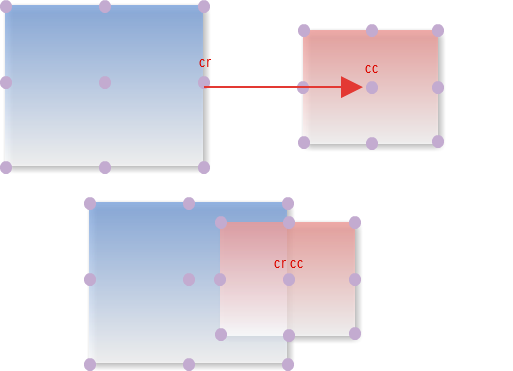
\includegraphics{align1.png}
\end{notice}
\end{quote}

\end{fulllineitems}


\index{effect (in module Overlay)}

\begin{fulllineitems}
\phantomsection\label{api/component/overlay/overlay:Overlay.effect}\pysigline{\code{Overlay.}\bfcode{effect}}{}~New in version 1.2: 类型对象。显示或隐藏时的特效支持,包括以下属性:
\index{effect (in module Overlay)}

\begin{fulllineitems}
\pysigline{\code{Overlay.}\bfcode{effect}}{}
类型string,可取值 \code{none} (无特效), \code{fade} (渐隐显示), \code{slide} (滑动显示)。默认 \code{none}

\end{fulllineitems}


\index{easing (in module Overlay)}

\begin{fulllineitems}
\phantomsection\label{api/component/overlay/overlay:Overlay.easing}\pysigline{\code{Overlay.}\bfcode{easing}}{}
同 {\hyperref[api/core/anim/index:Anim.Anim]{\code{Anim}}} 的 easing 参数配置。

\end{fulllineitems}


\index{duration (in module Overlay)}

\begin{fulllineitems}
\phantomsection\label{api/component/overlay/overlay:Overlay.duration}\pysigline{\code{Overlay.}\bfcode{duration}}{}
类型 number,动画持续时间,以秒为单元

\end{fulllineitems}


\end{fulllineitems}


\index{resize (in module Overlay)}

\begin{fulllineitems}
\phantomsection\label{api/component/overlay/overlay:Overlay.resize}\pysigline{\code{Overlay.}\bfcode{resize}}{}~New in version 1.2: (optional): 类型对象,拖动调整大小的配置,例如:
\begin{Verbatim}[commandchars=\\\{\}]
\PYG{p}{\PYGZob{}}
    \PYG{n+nx}{minWidth}\PYG{o}{:}\PYG{l+m+mi}{100}\PYG{p}{,} \PYG{c+c1}{//类型整数,表示拖动调整大小的最小宽度}
    \PYG{n+nx}{maxWidth}\PYG{o}{:}\PYG{l+m+mi}{1000}\PYG{p}{,} \PYG{c+c1}{//类型整数,表示拖动调整大小的最大宽度}
    \PYG{n+nx}{minHeight}\PYG{o}{:}\PYG{l+m+mi}{100}\PYG{p}{,} \PYG{c+c1}{//类型整数,表示拖动调整大小的最小高度}
    \PYG{n+nx}{maxHeight}\PYG{o}{:}\PYG{l+m+mi}{1000}\PYG{p}{,} \PYG{c+c1}{//类型整数,表示拖动调整大小的最大高度}
    \PYG{n+nx}{handlers}\PYG{o}{:}\PYG{p}{[}\PYG{l+s+s2}{"b"}\PYG{p}{,}\PYG{l+s+s2}{"t"}\PYG{p}{,}\PYG{l+s+s2}{"r"}\PYG{p}{,}\PYG{l+s+s2}{"l"}\PYG{p}{,}\PYG{l+s+s2}{"tr"}\PYG{p}{,}\PYG{l+s+s2}{"tl"}\PYG{p}{,}\PYG{l+s+s2}{"br"}\PYG{p}{,}\PYG{l+s+s2}{"bl"}\PYG{p}{]} \PYG{c+c1}{//类型字符串数组,取自上述 8 个值的集合。}
\PYG{p}{\PYGZcb{}}
\end{Verbatim}

\code{handlers} 配置表示的数组元素可取上述八种值之一,t,b,l,r 分别表示 top,bottom,left,right,加上组合共八种取值,
可在上,下,左,右以及左上,左下,右上,右下进行拖动。

\end{fulllineitems}



\paragraph{实例属性}
\label{api/component/overlay/overlay:id3}
当根据配置实例化 overlay 得到当前实例后,可调用实例上的 get 方法得到实例的特定属性以及 set 方法设置属性的值,例如
\begin{quote}

\begin{Verbatim}[commandchars=\\\{\}]
\PYG{k+kd}{var} \PYG{n+nx}{o} \PYG{o}{=} \PYG{k}{new} \PYG{n+nx}{Overlay}\PYG{p}{(}\PYG{p}{\PYGZob{}} \PYG{n+nx}{xy} \PYG{o}{:} \PYG{p}{[}\PYG{l+m+mi}{400}\PYG{p}{,}\PYG{l+m+mi}{200}\PYG{p}{]} \PYG{p}{\PYGZcb{}}\PYG{p}{)}\PYG{p}{;}
\PYG{c+c1}{//alert 当前实例的绝对坐标}
\PYG{n+nx}{alert}\PYG{p}{(}\PYG{n+nx}{o}\PYG{p}{.}\PYG{n+nx}{get}\PYG{p}{(}\PYG{l+s+s2}{"xy"}\PYG{p}{)}\PYG{p}{)}\PYG{p}{;}
\PYG{n+nx}{o}\PYG{p}{.}\PYG{n+nx}{set}\PYG{p}{(}\PYG{l+s+s2}{"xy"}\PYG{p}{,}\PYG{p}{[}\PYG{l+m+mi}{100}\PYG{p}{,}\PYG{l+m+mi}{200}\PYG{p}{]}\PYG{p}{)}\PYG{p}{;}
\PYG{c+c1}{//alert 当前实例新的绝对坐标}
\PYG{n+nx}{alert}\PYG{p}{(}\PYG{n+nx}{o}\PYG{p}{.}\PYG{n+nx}{get}\PYG{p}{(}\PYG{l+s+s2}{"xy"}\PYG{p}{)}\PYG{p}{)}\PYG{p}{;}
\end{Verbatim}
\end{quote}


\subparagraph{可获取属性列表}
\label{api/component/overlay/overlay:id4}
\index{x (in module Overlay)}

\begin{fulllineitems}
\pysigline{\code{Overlay.}\bfcode{x}}{}
(读写):相对于页面绝对横坐标,类型参见配置

\end{fulllineitems}


\index{y (in module Overlay)}

\begin{fulllineitems}
\pysigline{\code{Overlay.}\bfcode{y}}{}
(读写):相对于页面绝对纵坐标,类型参见配置

\end{fulllineitems}


\index{xy (in module Overlay)}

\begin{fulllineitems}
\pysigline{\code{Overlay.}\bfcode{xy}}{}
(读写):相当与一次同时读写 {\hyperref[api/component/overlay/overlay:Overlay.x]{\code{x}}} 和 {\hyperref[api/component/overlay/overlay:Overlay.y]{\code{y}}} 属性,类型参见配置

\end{fulllineitems}


\index{align (in module Overlay)}

\begin{fulllineitems}
\pysigline{\code{Overlay.}\bfcode{align}}{}
(读写):弹出层的对齐信息,类型参见配置

\end{fulllineitems}


\index{visible (in module Overlay)}

\begin{fulllineitems}
\phantomsection\label{api/component/overlay/overlay:Overlay.visible}\pysigline{\code{Overlay.}\bfcode{visible}}{}
(读写):弹出层的显示与否,类型 boolean

\end{fulllineitems}


\index{el (in module Overlay)}

\begin{fulllineitems}
\phantomsection\label{api/component/overlay/overlay:Overlay.el}\pysigline{\code{Overlay.}\bfcode{el}}{}
(只读):获取弹出层的根节点,类型 \code{KISSY.Node} 。

\begin{notice}{note}{Note:}
必须在调用 {\hyperref[api/component/overlay/overlay:Overlay.Overlay.render]{\code{render()}}} 方法之后才可以获取
\end{notice}

\end{fulllineitems}


\index{contentEl (in module Overlay)}

\begin{fulllineitems}
\phantomsection\label{api/component/overlay/overlay:Overlay.contentEl}\pysigline{\code{Overlay.}\bfcode{contentEl}}{}
(只读):获取弹出层真正内容所在的节点,类型 \code{KISSY.Node} 。

\begin{notice}{note}{Note:}
必须在调用  {\hyperref[api/component/overlay/overlay:Overlay.Overlay.render]{\code{render()}}} 方法之后才可以获取。
\end{notice}

弹出层的 html 结构如下

\begin{Verbatim}[commandchars=\\\{\}]
\PYG{n+nt}{\textless{}div}\PYG{n+nt}{\textgreater{}}\PYG{c}{\textless{}!--}\PYG{c}{ 弹出层根节点 }\PYG{c}{--\textgreater{}}
    \PYG{n+nt}{\textless{}div}\PYG{n+nt}{\textgreater{}}\PYG{c}{\textless{}!--}\PYG{c}{ 弹出层内容节点 }\PYG{c}{-}\PYG{c}{--\textgreater{}}
        \PYG{c}{\textless{}!--}\PYG{c}{ 弹出层真正内容所在 }\PYG{c}{--\textgreater{}}
    \PYG{n+nt}{\textless{}/div\textgreater{}}
\PYG{n+nt}{\textless{}/div\textgreater{}}
\end{Verbatim}

一般调用弹出层的 {\hyperref[api/component/overlay/overlay:Overlay.Overlay.render]{\code{render()}}} 方法后,可通过获取 {\hyperref[api/component/overlay/overlay:Overlay.contentEl]{\code{contentEl}}} 属性获取内容所在节点,来动态修改弹出层的内容。

\end{fulllineitems}



\paragraph{实例方法}
\label{api/component/overlay/overlay:id5}
\index{render() (Overlay.Overlay method)}

\begin{fulllineitems}
\phantomsection\label{api/component/overlay/overlay:Overlay.Overlay.render}\pysiglinewithargsret{\code{Overlay.}\bfcode{render}}{}{}
渲染当前实例,生成对应的 dom 节点并添加到页面文档树中。

\begin{notice}{note}{Note:}
取 {\hyperref[api/component/overlay/overlay:Overlay.el]{\code{el}}} 与 {\hyperref[api/component/overlay/overlay:Overlay.contentEl]{\code{contentEl}}} 属性值前必须调用过该方法。
\end{notice}

\end{fulllineitems}


\index{show() (Overlay.Overlay method)}

\begin{fulllineitems}
\phantomsection\label{api/component/overlay/overlay:Overlay.Overlay.show}\pysiglinewithargsret{\code{Overlay.}\bfcode{show}}{}{}
显示弹窗,位置根据 {\hyperref[api/component/overlay/overlay:Overlay.align]{\code{align}}} 或者 {\hyperref[api/component/overlay/overlay:Overlay.xy]{\code{xy}}} 确定。

\end{fulllineitems}


\index{hide() (Overlay.Overlay method)}

\begin{fulllineitems}
\phantomsection\label{api/component/overlay/overlay:Overlay.Overlay.hide}\pysiglinewithargsret{\code{Overlay.}\bfcode{hide}}{}{}
隐藏弹窗

\end{fulllineitems}


\index{align() (Overlay.Overlay method)}

\begin{fulllineitems}
\phantomsection\label{api/component/overlay/overlay:Overlay.Overlay.align}\pysiglinewithargsret{\code{Overlay.}\bfcode{align}}{\emph{node}, \emph{points}, \emph{offset}}{}~\begin{quote}\begin{description}
\item[{Parameters}] \leavevmode\begin{itemize}
\item {}
\textbf{node} (\emph{string\textbar{}KISSY.Node\textbar{}HTMLDOMNode}) -- 类型对齐的参考元素

\item {}
\textbf{points} (\emph{Array\textless{}string\textgreater{}}) -- 对齐的参考位置

\item {}
\textbf{offset} (\emph{Array\textless{}number\textgreater{}}) -- 相对对齐元素的偏移

\end{itemize}

\end{description}\end{quote}

相当于调用

\begin{Verbatim}[commandchars=\\\{\}]
\PYG{n+nx}{set}\PYG{p}{(}\PYG{l+s+s2}{"align"}\PYG{p}{,}\PYG{p}{\PYGZob{}}
    \PYG{n+nx}{node}\PYG{o}{:} \PYG{n+nx}{node}\PYG{p}{,}
    \PYG{n+nx}{points}\PYG{o}{:} \PYG{n+nx}{points}\PYG{p}{,}
    \PYG{n+nx}{offset}\PYG{o}{:} \PYG{n+nx}{offset}
\PYG{p}{\PYGZcb{}}\PYG{p}{)}\PYG{p}{;}
\end{Verbatim}

\begin{notice}{note}{Note:}
调用该方法前请先调用 {\hyperref[api/component/overlay/overlay:Overlay.Overlay.render]{\code{render()}}}.
\end{notice}

\end{fulllineitems}


\index{center() (Overlay.Overlay method)}

\begin{fulllineitems}
\phantomsection\label{api/component/overlay/overlay:Overlay.Overlay.center}\pysiglinewithargsret{\code{Overlay.}\bfcode{center}}{}{}
将弹出层放在当前视窗中央。

\begin{notice}{note}{Note:}
调用该方法前请先调用 {\hyperref[api/component/overlay/overlay:Overlay.Overlay.render]{\code{render()}}}.
\end{notice}

\end{fulllineitems}


\index{move() (Overlay.Overlay method)}

\begin{fulllineitems}
\phantomsection\label{api/component/overlay/overlay:Overlay.Overlay.move}\pysiglinewithargsret{\code{Overlay.}\bfcode{move}}{\emph{x}, \emph{y}}{}~\begin{quote}\begin{description}
\item[{Parameters}] \leavevmode\begin{itemize}
\item {}
\textbf{x} (\emph{number}) -- 相对文档左上角横坐标

\item {}
\textbf{y} (\emph{number}) -- 相对文档左上角纵坐标

\end{itemize}

\end{description}\end{quote}

相当于调用

\begin{Verbatim}[commandchars=\\\{\}]
\PYG{n+nx}{set}\PYG{p}{(}\PYG{l+s+s2}{"xy"}\PYG{p}{,}\PYG{p}{[}\PYG{n+nx}{x}\PYG{p}{,}\PYG{n+nx}{y}\PYG{p}{]}\PYG{p}{)}\PYG{p}{;}
\end{Verbatim}

\end{fulllineitems}



\paragraph{触发事件}
\label{api/component/overlay/overlay:id6}
\index{hide (in module Overlay)}

\begin{fulllineitems}
\phantomsection\label{api/component/overlay/overlay:Overlay.hide}\pysigline{\code{Overlay.}\bfcode{hide}}{}
当弹出层隐藏时触发

\end{fulllineitems}


\index{show (in module Overlay)}

\begin{fulllineitems}
\phantomsection\label{api/component/overlay/overlay:Overlay.show}\pysigline{\code{Overlay.}\bfcode{show}}{}
当弹出层显示时触发

\end{fulllineitems}


\index{beforeVisibleChange (in module Overlay)}

\begin{fulllineitems}
\phantomsection\label{api/component/overlay/overlay:Overlay.beforeVisibleChange}\pysigline{\code{Overlay.}\bfcode{beforeVisibleChange}}{}
当弹出层隐藏或显示前触发,传给事件处理函数的参数为一个对象,格式如下:

\begin{Verbatim}[commandchars=\\\{\}]
\PYG{p}{\PYGZob{}}
    \PYG{n+nx}{newVal} \PYG{o}{:} \PYG{c+c1}{// 类型 boolean,将要隐藏时为 false,将要显示时为 true}
    \PYG{n+nx}{prevVal} \PYG{o}{:} \PYG{c+c1}{// 类型 boolean,当前弹出层显示与否}
\PYG{p}{\PYGZcb{}}
\end{Verbatim}

\begin{notice}{note}{Note:}
当该事件的函数处理器返回 false ,则会阻止将要进行的显示或隐藏动作。
\end{notice}

\end{fulllineitems}



\subsubsection{子类 Dialog}
\label{api/component/overlay/dialog::doc}\label{api/component/overlay/dialog:dialog}

\paragraph{获取对话框构造器}
\label{api/component/overlay/dialog:id1}
页面引入 kissy.js :

\begin{Verbatim}[commandchars=\\\{\}]
\PYG{n+nt}{\textless{}script }\PYG{n+na}{src=}\PYG{l+s}{'kissy.js'}\PYG{n+nt}{\textgreater{}}\PYG{n+nt}{\textless{}/script\textgreater{}}
\end{Verbatim}

Dialog 属于 overlay 模块,通过 use 加载 overlay 模块:

\begin{Verbatim}[commandchars=\\\{\}]
\PYG{n+nx}{KISSY}\PYG{p}{.}\PYG{n+nx}{use}\PYG{p}{(}\PYG{l+s+s2}{"overlay"}\PYG{p}{,}\PYG{k+kd}{function}\PYG{p}{(}\PYG{p}{)}\PYG{p}{\PYGZob{}}
    \PYG{k+kd}{var} \PYG{n+nx}{Dialog}\PYG{o}{=}\PYG{n+nx}{S}\PYG{p}{.}\PYG{n+nx}{Dialog}\PYG{p}{;}
    \PYG{c+c1}{//使用 Dialog 构造器}
\PYG{p}{\PYGZcb{}}\PYG{p}{)}\PYG{p}{;}
\end{Verbatim}
New in version 1.2: KISSY 1.2 可直接通过依赖注入,从函数参数中取得
\begin{Verbatim}[commandchars=\\\{\}]
\PYG{n+nx}{KISSY}\PYG{p}{.}\PYG{n+nx}{use}\PYG{p}{(}\PYG{l+s+s2}{"overlay"}\PYG{p}{,}\PYG{k+kd}{function}\PYG{p}{(}\PYG{n+nx}{S}\PYG{p}{,}\PYG{n+nx}{Overlay}\PYG{p}{)}\PYG{p}{\PYGZob{}}
    \PYG{c+c1}{//使用 Overlay 构造器}
    \PYG{k+kd}{var} \PYG{n+nx}{Dialog}\PYG{o}{=}\PYG{n+nx}{Overlay}\PYG{p}{.}\PYG{n+nx}{Dialog}\PYG{p}{;}
\PYG{p}{\PYGZcb{}}\PYG{p}{)}\PYG{p}{;}
\end{Verbatim}


\paragraph{构造器接口}
\label{api/component/overlay/dialog:id2}
\index{Dialog (class in Overlay)}

\begin{fulllineitems}
\phantomsection\label{api/component/overlay/dialog:Overlay.Dialog}\pysiglinewithargsret{\strong{class }\code{Overlay.}\bfcode{Dialog}}{\emph{config}}{}~\begin{quote}\begin{description}
\item[{Parameters}] \leavevmode
\textbf{config} (\emph{object}) -- 类型对象,实例对象所需的配置

\end{description}\end{quote}

例如一个简单的配置项:

\begin{Verbatim}[commandchars=\\\{\}]
\PYG{p}{\PYGZob{}}
    \PYG{n+nx}{width}\PYG{o}{:}\PYG{l+s+s2}{"200px"}\PYG{p}{,}
    \PYG{n+nx}{render}\PYG{o}{:}\PYG{l+s+s2}{"\#container"}
\PYG{p}{\PYGZcb{}}
\end{Verbatim}

\end{fulllineitems}



\subparagraph{对话框的 DOM 结构}
\label{api/component/overlay/dialog:dom}
\begin{Verbatim}[commandchars=\\\{\}]
\PYG{n+nt}{\textless{}div}\PYG{n+nt}{\textgreater{}} \PYG{c}{\textless{}!--}\PYG{c}{ 对话框根节点 }\PYG{c}{--\textgreater{}}
    \PYG{n+nt}{\textless{}div}\PYG{n+nt}{\textgreater{}} \PYG{c}{\textless{}!--}\PYG{c}{ 对话框内容节点 }\PYG{c}{--\textgreater{}}
        \PYG{n+nt}{\textless{}div}\PYG{n+nt}{\textgreater{}} \PYG{c}{\textless{}!--}\PYG{c}{ 对话框标题节点 }\PYG{c}{--\textgreater{}}
        \PYG{n+nt}{\textless{}/div\textgreater{}}

        \PYG{n+nt}{\textless{}div}\PYG{n+nt}{\textgreater{}} \PYG{c}{\textless{}!--}\PYG{c}{ 对话框体节点 }\PYG{c}{--\textgreater{}}
        \PYG{n+nt}{\textless{}/div\textgreater{}}

        \PYG{n+nt}{\textless{}div}\PYG{n+nt}{\textgreater{}} \PYG{c}{\textless{}!--}\PYG{c}{ 对话框底部节点 }\PYG{c}{--\textgreater{}}
        \PYG{n+nt}{\textless{}/div\textgreater{}}
    \PYG{n+nt}{\textless{}/div\textgreater{}}
\PYG{n+nt}{\textless{}/div\textgreater{}}
\end{Verbatim}


\subparagraph{config 配置项详解}
\label{api/component/overlay/dialog:config}
除了 {\hyperref[api/component/overlay/overlay:Overlay.content]{\code{content}}} 配置项外与 {\hyperref[api/component/overlay/overlay:Overlay.Overlay]{\code{Overlay}}} 的配置项完全相同,但是 {\hyperref[api/component/overlay/dialog:Overlay.Dialog]{\code{Dialog}}} 新增了一些配置项,如下所示:

\index{headerContent (in module Overlay)}

\begin{fulllineitems}
\phantomsection\label{api/component/overlay/dialog:Overlay.headerContent}\pysigline{\code{Overlay.}\bfcode{headerContent}}{}
类型字符串,对话框的标题 html.

\end{fulllineitems}


\index{bodyContent (in module Overlay)}

\begin{fulllineitems}
\phantomsection\label{api/component/overlay/dialog:Overlay.bodyContent}\pysigline{\code{Overlay.}\bfcode{bodyContent}}{}
类型字符串,对话框的体 html。

\end{fulllineitems}


\index{footerContent (in module Overlay)}

\begin{fulllineitems}
\phantomsection\label{api/component/overlay/dialog:Overlay.footerContent}\pysigline{\code{Overlay.}\bfcode{footerContent}}{}
类型字符串,对话框的底部 html。

\end{fulllineitems}


\index{closable (in module Overlay)}

\begin{fulllineitems}
\phantomsection\label{api/component/overlay/dialog:Overlay.closable}\pysigline{\code{Overlay.}\bfcode{closable}}{}
类型 boolean,对话框右上角是否包括关闭按钮

\end{fulllineitems}


\index{draggable (in module Overlay)}

\begin{fulllineitems}
\phantomsection\label{api/component/overlay/dialog:Overlay.draggable}\pysigline{\code{Overlay.}\bfcode{draggable}}{}
类型 boolean,是否允许拖动头部移动,注意启用时需同时 \code{use("dd")} ,例如

\begin{Verbatim}[commandchars=\\\{\}]
\PYG{n+nx}{KISSY}\PYG{p}{.}\PYG{n+nx}{use}\PYG{p}{(}\PYG{l+s+s2}{"dd,overlay"}\PYG{p}{,}\PYG{k+kd}{function}\PYG{p}{(}\PYG{n+nx}{S}\PYG{p}{,}\PYG{n+nx}{DD}\PYG{p}{,}\PYG{n+nx}{Overlay}\PYG{p}{)}\PYG{p}{\PYGZob{}}
    \PYG{k}{new} \PYG{n+nx}{Overlay}\PYG{p}{.}\PYG{n+nx}{Dialog}\PYG{p}{(}\PYG{p}{\PYGZob{}}
        \PYG{n+nx}{draggable} \PYG{o}{:} \PYG{k+kc}{true}
    \PYG{p}{\PYGZcb{}}\PYG{p}{)}\PYG{p}{;}
\PYG{p}{\PYGZcb{}}\PYG{p}{)}\PYG{p}{;}
\end{Verbatim}

\end{fulllineitems}


\index{aria (in module Overlay)}

\begin{fulllineitems}
\phantomsection\label{api/component/overlay/dialog:Overlay.aria}\pysigline{\code{Overlay.}\bfcode{aria}}{}~New in version 1.2: 类型 boolean,是否开启 aria 支持。默认 false 。开启后,窗口显示出来时自动获得焦点并且 tab 键只能在窗口内部转移焦点。
\end{fulllineitems}


\index{constrain (in module Overlay)}

\begin{fulllineitems}
\phantomsection\label{api/component/overlay/dialog:Overlay.constrain}\pysigline{\code{Overlay.}\bfcode{constrain}}{}
类型 boolean 或者选择器字符串 ,和 draggable 配合,限制拖动的范围,
\begin{itemize}
\item {}
取值 true 时,只能在当前视窗范围内拖动。

\item {}
取值选择器字符串时,则在限制拖动范围为根据该选择器字符串取到的第一个节点所在区域。

\item {}
取值 false 时,可任意移动,例如:

\end{itemize}

\begin{Verbatim}[commandchars=\\\{\}]
\PYG{n+nx}{KISSY}\PYG{p}{.}\PYG{n+nx}{use}\PYG{p}{(}\PYG{l+s+s2}{"dd,overlay"}\PYG{p}{,}\PYG{k+kd}{function}\PYG{p}{(}\PYG{n+nx}{S}\PYG{p}{,}\PYG{n+nx}{DD}\PYG{p}{,}\PYG{n+nx}{Overlay}\PYG{p}{)}\PYG{p}{\PYGZob{}}
    \PYG{k}{new} \PYG{n+nx}{Overlay}\PYG{p}{.}\PYG{n+nx}{Dialog}\PYG{p}{(}\PYG{p}{\PYGZob{}}
        \PYG{n+nx}{draggable} \PYG{o}{:} \PYG{k+kc}{true}\PYG{p}{,}
        \PYG{n+nx}{contrain}\PYG{o}{:}\PYG{k+kc}{true} \PYG{c+c1}{// 限制拖动区域为当前视窗范围}
    \PYG{p}{\PYGZcb{}}\PYG{p}{)}\PYG{p}{;}
\PYG{p}{\PYGZcb{}}\PYG{p}{)}\PYG{p}{;}

\PYG{n+nx}{KISSY}\PYG{p}{.}\PYG{n+nx}{use}\PYG{p}{(}\PYG{l+s+s2}{"dd,overlay"}\PYG{p}{,}\PYG{k+kd}{function}\PYG{p}{(}\PYG{n+nx}{S}\PYG{p}{,}\PYG{n+nx}{DD}\PYG{p}{,}\PYG{n+nx}{Overlay}\PYG{p}{)}\PYG{p}{\PYGZob{}}
    \PYG{k}{new} \PYG{n+nx}{Overlay}\PYG{p}{.}\PYG{n+nx}{Dialog}\PYG{p}{(}\PYG{p}{\PYGZob{}}
        \PYG{n+nx}{draggable} \PYG{o}{:} \PYG{k+kc}{true}\PYG{p}{,}
        \PYG{n+nx}{contrain}\PYG{o}{:}\PYG{l+s+s2}{"\#container"} \PYG{c+c1}{// 限制拖动区域为 container 节点所占据区域}
    \PYG{p}{\PYGZcb{}}\PYG{p}{)}\PYG{p}{;}
\PYG{p}{\PYGZcb{}}\PYG{p}{)}\PYG{p}{;}
\end{Verbatim}

\end{fulllineitems}



\paragraph{实例方法}
\label{api/component/overlay/dialog:id3}
同 {\hyperref[api/component/overlay/overlay:Overlay.Overlay]{\code{Overlay}}} 。


\paragraph{实例属性}
\label{api/component/overlay/dialog:id4}
对话框 Dialog 实例可以获得弹出层 Overlay 实例的所有属性,除此之外还有:

\index{header (in module Overlay)}

\begin{fulllineitems}
\phantomsection\label{api/component/overlay/dialog:Overlay.header}\pysigline{\code{Overlay.}\bfcode{header}}{}
(只读)类型 \code{KISSY.Node} ,获得对话框的头部节点。

\end{fulllineitems}


\index{body (in module Overlay)}

\begin{fulllineitems}
\phantomsection\label{api/component/overlay/dialog:Overlay.body}\pysigline{\code{Overlay.}\bfcode{body}}{}
(只读)类型 \code{KISSY.Node} ,获得对话框的体部节点。

\end{fulllineitems}


\index{footer (in module Overlay)}

\begin{fulllineitems}
\phantomsection\label{api/component/overlay/dialog:Overlay.footer}\pysigline{\code{Overlay.}\bfcode{footer}}{}
(只读): 类型 \code{KISSY.Node} ,获得对话框的底部节点。

\end{fulllineitems}


\begin{notice}{note}{Note:}
以上三个属性在获取前必须调用过 \code{render()} 方法。
\end{notice}

\index{closable (in module Overlay)}

\begin{fulllineitems}
\pysigline{\code{Overlay.}\bfcode{closable}}{}
(读写)同相应配置项,设置右上角拖放区域有无。

\end{fulllineitems}


\index{draggable (in module Overlay)}

\begin{fulllineitems}
\pysigline{\code{Overlay.}\bfcode{draggable}}{}
(读写)同相应配置项,设置头部是否可以拖放。

\end{fulllineitems}


\index{constrain (in module Overlay)}

\begin{fulllineitems}
\pysigline{\code{Overlay.}\bfcode{constrain}}{}
(读写)同相应配置项,设置拖放区域范围。

\end{fulllineitems}



\paragraph{触发事件}
\label{api/component/overlay/dialog:id5}
同弹出层 {\hyperref[api/component/overlay/overlay:Overlay.Overlay]{\code{Overlay}}} ,包括 {\hyperref[api/component/overlay/overlay:Overlay.show]{\code{show}}} , {\hyperref[api/component/overlay/overlay:Overlay.hide]{\code{hide}}} , {\hyperref[api/component/overlay/overlay:Overlay.beforeVisibleChange]{\code{beforeVisibleChange}}} .


\subsubsection{子类 Popup}
\label{api/component/overlay/popup:popup}\label{api/component/overlay/popup::doc}

\paragraph{获取对话框构造器}
\label{api/component/overlay/popup:id1}
页面引入 kissy.js :

\begin{Verbatim}[commandchars=\\\{\}]
\PYG{n+nt}{\textless{}script }\PYG{n+na}{src=}\PYG{l+s}{'kissy.js'}\PYG{n+nt}{\textgreater{}}\PYG{n+nt}{\textless{}/script\textgreater{}}
\end{Verbatim}

Popup 属于 overlay 模块, 通过 use 加载 overlay 模块:

\begin{Verbatim}[commandchars=\\\{\}]
\PYG{n+nx}{KISSY}\PYG{p}{.}\PYG{n+nx}{use}\PYG{p}{(}\PYG{l+s+s2}{"overlay"}\PYG{p}{,}\PYG{k+kd}{function}\PYG{p}{(}\PYG{p}{)}\PYG{p}{\PYGZob{}}
    \PYG{k+kd}{var} \PYG{n+nx}{Popup} \PYG{o}{=} \PYG{n+nx}{S}\PYG{p}{.}\PYG{n+nx}{Popup}\PYG{p}{;}
    \PYG{c+c1}{// 使用 Popup 构造器}
\PYG{p}{\PYGZcb{}}\PYG{p}{)}\PYG{p}{;}
\end{Verbatim}
New in version 1.2: KISSY 1.2 可直接通过依赖注入, 从函数参数中取得
\begin{Verbatim}[commandchars=\\\{\}]
\PYG{n+nx}{KISSY}\PYG{p}{.}\PYG{n+nx}{use}\PYG{p}{(}\PYG{l+s+s2}{"overlay"}\PYG{p}{,}\PYG{k+kd}{function}\PYG{p}{(}\PYG{n+nx}{S}\PYG{p}{,}\PYG{n+nx}{Overlay}\PYG{p}{)}\PYG{p}{\PYGZob{}}
    \PYG{c+c1}{//使用 Popup 构造器}
    \PYG{k+kd}{var} \PYG{n+nx}{Popup} \PYG{o}{=} \PYG{n+nx}{Overlay}\PYG{p}{.}\PYG{n+nx}{Popup}\PYG{p}{;}
\PYG{p}{\PYGZcb{}}\PYG{p}{)}\PYG{p}{;}
\end{Verbatim}


\paragraph{构造器接口}
\label{api/component/overlay/popup:id2}
\index{Popup (class in Overlay)}

\begin{fulllineitems}
\phantomsection\label{api/component/overlay/popup:Overlay.Popup}\pysiglinewithargsret{\strong{class }\code{Overlay.}\bfcode{Popup}}{\emph{container}, \emph{config}}{}~\begin{quote}\begin{description}
\item[{Parameters}] \leavevmode
\textbf{container} (\emph{object}) --
容器对象, 可取:
\begin{itemize}
\item {}
选择器字符串, 此时会取第一个节点作为弹出层的根节点;

\item {}
HTMLElement 或直接传入 KISSY Node 对象;

\item {}
也可不设置, 此时, 表示新建 HTMLElement;

\end{itemize}
\begin{quote}\begin{description}
\item[{param object config}] \leavevmode
类型对象, 实例对象所需的配置

\end{description}\end{quote}


\end{description}\end{quote}

例如一个简单的配置项:

\begin{Verbatim}[commandchars=\\\{\}]
\PYG{p}{\PYGZob{}}
    \PYG{n+nx}{width}\PYG{o}{:}\PYG{l+s+s2}{"200px"}\PYG{p}{,}
    \PYG{n+nx}{render}\PYG{o}{:}\PYG{l+s+s2}{"\#container"}
\PYG{p}{\PYGZcb{}}
\end{Verbatim}

\end{fulllineitems}



\subparagraph{config 配置项详解}
\label{api/component/overlay/popup:config}
与 {\hyperref[api/component/overlay/overlay:Overlay.Overlay]{\code{Overlay}}} 的配置项完全相同, 除此之外, 还有:

\index{trigger (in module Overlay)}

\begin{fulllineitems}
\phantomsection\label{api/component/overlay/popup:Overlay.trigger}\pysigline{\code{Overlay.}\bfcode{trigger}}{}
指定触发器, 类型为 选择器字符串 或 \code{HTMLElement} 或 \code{KISSY Node} 对象

\begin{Verbatim}[commandchars=\\\{\}]
\PYG{n+nx}{KISSY}\PYG{p}{.}\PYG{n+nx}{use}\PYG{p}{(}\PYG{l+s+s2}{"dd,overlay"}\PYG{p}{,}\PYG{k+kd}{function}\PYG{p}{(}\PYG{n+nx}{S}\PYG{p}{,}\PYG{n+nx}{DD}\PYG{p}{,}\PYG{n+nx}{Overlay}\PYG{p}{)}\PYG{p}{\PYGZob{}}
    \PYG{k}{new} \PYG{n+nx}{Overlay}\PYG{p}{.}\PYG{n+nx}{Dialog}\PYG{p}{(}\PYG{p}{\PYGZob{}}
        \PYG{n+nx}{draggable} \PYG{o}{:} \PYG{k+kc}{true}\PYG{p}{,}
        \PYG{n+nx}{contrain}\PYG{o}{:}\PYG{k+kc}{true} \PYG{c+c1}{// 限制拖动区域为当前视窗范围}
    \PYG{p}{\PYGZcb{}}\PYG{p}{)}\PYG{p}{;}
\PYG{p}{\PYGZcb{}}\PYG{p}{)}\PYG{p}{;}

\PYG{n+nx}{KISSY}\PYG{p}{.}\PYG{n+nx}{use}\PYG{p}{(}\PYG{l+s+s2}{"dd,overlay"}\PYG{p}{,}\PYG{k+kd}{function}\PYG{p}{(}\PYG{n+nx}{S}\PYG{p}{,}\PYG{n+nx}{DD}\PYG{p}{,}\PYG{n+nx}{Overlay}\PYG{p}{)}\PYG{p}{\PYGZob{}}
    \PYG{k}{new} \PYG{n+nx}{Overlay}\PYG{p}{.}\PYG{n+nx}{Dialog}\PYG{p}{(}\PYG{p}{\PYGZob{}}
        \PYG{n+nx}{draggable} \PYG{o}{:} \PYG{k+kc}{true}\PYG{p}{,}
        \PYG{n+nx}{contrain}\PYG{o}{:}\PYG{l+s+s2}{"\#container"} \PYG{c+c1}{// 限制拖动区域为 container 节点所占据区域}
    \PYG{p}{\PYGZcb{}}\PYG{p}{)}\PYG{p}{;}
\PYG{p}{\PYGZcb{}}\PYG{p}{)}\PYG{p}{;}
\end{Verbatim}

\end{fulllineitems}


\index{triggerType (in module Overlay)}

\begin{fulllineitems}
\phantomsection\label{api/component/overlay/popup:Overlay.triggerType}\pysigline{\code{Overlay.}\bfcode{triggerType}}{}
触发类型, 可取 `click', `mouse', 默认为 `click'.
\begin{itemize}
\item {}
取 `click' 时, 表示当点击触发器元素时, 显示弹出层;

\item {}
取 `mouse' 时, 表示当鼠标移入触发器元素时, 显示弹出层, 当鼠标离开触发器元素时, 隐藏弹出层;

\end{itemize}

\end{fulllineitems}



\paragraph{实例方法}
\label{api/component/overlay/popup:id3}
同 {\hyperref[api/component/overlay/overlay:Overlay.Overlay]{\code{Overlay}}}.


\paragraph{实例属性}
\label{api/component/overlay/popup:id4}
同 {\hyperref[api/component/overlay/overlay:Overlay.Overlay]{\code{Overlay}}}.


\paragraph{触发事件}
\label{api/component/overlay/popup:id5}
同 {\hyperref[api/component/overlay/overlay:Overlay.Overlay]{\code{Overlay}}}, 包括 {\hyperref[api/component/overlay/overlay:Overlay.show]{\code{show}}} , {\hyperref[api/component/overlay/overlay:Overlay.hide]{\code{hide}}} , {\hyperref[api/component/overlay/overlay:Overlay.beforeVisibleChange]{\code{beforeVisibleChange}}} .
\phantomsection\label{api/component/switchable/index:module-Switchable}
\index{Switchable (module)}

\subsection{Switchable}
\label{api/component/switchable/index::doc}\label{api/component/switchable/index:switchable}
by \href{mailto:lifesinger@gmail.com}{玉伯}

\begin{notice}{important}{Important:}
该模块由 Switchable 基础类、插件和 Widget 类组成。Switchable 基础类抽象了切换的基本操作,通过插件机制实现了自动播放、循环、切换效果、延迟加载、倒计时动画等扩展功能,最后封装成各个 Widget 类,让用户能简明快速地调用。
\end{notice}


\subsubsection{父类 Switchable}
\label{api/component/switchable/switchable::doc}\label{api/component/switchable/switchable:switchable}
\begin{notice}{hint}{Hint:}
Switchable 是核心类, S.Tabs/S.Slide/S.Accordion/S.Carousel 都是扩展自它.
\end{notice}


\paragraph{获取构造器}
\label{api/component/switchable/switchable:id1}
页面引入 kissy.js :

\begin{Verbatim}[commandchars=\\\{\}]
\PYG{n+nt}{\textless{}script }\PYG{n+na}{src=}\PYG{l+s}{'kissy.js'}\PYG{n+nt}{\textgreater{}}\PYG{n+nt}{\textless{}/script\textgreater{}}
\end{Verbatim}

通过 use 加载 Switchable 模块:

\begin{Verbatim}[commandchars=\\\{\}]
\PYG{n+nx}{KISSY}\PYG{p}{.}\PYG{n+nx}{use}\PYG{p}{(}\PYG{l+s+s2}{"switchable"}\PYG{p}{,}\PYG{k+kd}{function}\PYG{p}{(}\PYG{p}{)}\PYG{p}{\PYGZob{}}
    \PYG{k+kd}{var} \PYG{n+nx}{Switchable} \PYG{o}{=} \PYG{n+nx}{S}\PYG{p}{.}\PYG{n+nx}{Switchable}\PYG{p}{;}
    \PYG{c+c1}{//使用 Switchable 构造器}
\PYG{p}{\PYGZcb{}}\PYG{p}{)}\PYG{p}{;}
\end{Verbatim}
New in version 1.2: KISSY 1.2 可直接通过依赖注入,从函数参数中取得
\begin{Verbatim}[commandchars=\\\{\}]
\PYG{n+nx}{KISSY}\PYG{p}{.}\PYG{n+nx}{use}\PYG{p}{(}\PYG{l+s+s2}{"switchable"}\PYG{p}{,}\PYG{k+kd}{function}\PYG{p}{(}\PYG{n+nx}{S}\PYG{p}{,}\PYG{n+nx}{Switchable}\PYG{p}{)}\PYG{p}{\PYGZob{}}
    \PYG{c+c1}{//使用 Switchable 构造器}
\PYG{p}{\PYGZcb{}}\PYG{p}{)}\PYG{p}{;}
\end{Verbatim}


\paragraph{构造器接口}
\label{api/component/switchable/switchable:id2}
\index{Switchable (class in Switchable)}

\begin{fulllineitems}
\phantomsection\label{api/component/switchable/switchable:Switchable.Switchable}\pysiglinewithargsret{\strong{class }\code{Switchable.}\bfcode{Switchable}}{\emph{container}, \emph{config}}{}~\begin{quote}\begin{description}
\item[{Parameters}] \leavevmode\begin{itemize}
\item {}
\textbf{container} (\emph{object}) -- 所在容器, 可以是 选择器字符串, HTMLElement

\item {}
\textbf{config} (\emph{object}) -- Switchable 的配置信息, 具体见下详解

\end{itemize}

\end{description}\end{quote}

例如一个简单的接口示例:

\begin{Verbatim}[commandchars=\\\{\}]
\PYG{k+kd}{var} \PYG{n+nx}{a} \PYG{o}{=} \PYG{k}{new} \PYG{n+nx}{S}\PYG{p}{.}\PYG{n+nx}{Tabs}\PYG{p}{(}\PYG{l+s+s1}{'\#J\PYGZus{}TSearch'}\PYG{p}{,} \PYG{p}{\PYGZob{}}
    \PYG{n+nx}{markupType}\PYG{o}{:} \PYG{l+m+mi}{0}\PYG{p}{,}
    \PYG{n+nx}{navCls}\PYG{o}{:} \PYG{l+s+s1}{'tsearch-tab'}\PYG{p}{,}
    \PYG{n+nx}{contentCls}\PYG{o}{:} \PYG{l+s+s1}{'tsearch-panel'}\PYG{p}{,}
    \PYG{n+nx}{triggerType}\PYG{o}{:} \PYG{l+s+s1}{'mouse'}\PYG{p}{,}
    \PYG{n+nx}{activeTriggerCls}\PYG{o}{:} \PYG{l+s+s1}{'current'}
\PYG{p}{\PYGZcb{}}\PYG{p}{)}\PYG{p}{;}
\end{Verbatim}

\end{fulllineitems}



\subparagraph{config 配置项详解}
\label{api/component/switchable/switchable:config}
\index{markupType (Switchable.Switchable attribute)}

\begin{fulllineitems}
\phantomsection\label{api/component/switchable/switchable:Switchable.Switchable.markupType}\pysigline{\code{Switchable.}\bfcode{markupType}}{}
(optional): \{Number\} 默认为0. 指明 DOM 结构标记的类型, 可取 0, 1, 2:

\end{fulllineitems}


当取 0 时, 表示 DOM 是默认结构: 通过 nav 和 content 来获取 triggers 和 panels, 即通过配置以下两个参数获取.

\index{navCls (Switchable.Switchable attribute)}

\begin{fulllineitems}
\phantomsection\label{api/component/switchable/switchable:Switchable.Switchable.navCls}\pysigline{\code{Switchable.}\bfcode{navCls}}{}
(optional): \{String\}, triggers 所在容器的 class, 默认为 `ks-switchable-nav',

\end{fulllineitems}


\index{contentCls (Switchable.Switchable attribute)}

\begin{fulllineitems}
\phantomsection\label{api/component/switchable/switchable:Switchable.Switchable.contentCls}\pysigline{\code{Switchable.}\bfcode{contentCls}}{}
(optional): \{String\}, panels 所在容器的 class, 默认为 `ks-switchable-content',

\end{fulllineitems}


这种方式的 DOM 结构类似于:
\begin{quote}

\begin{Verbatim}[commandchars=\\\{\}]
\PYG{n+nt}{\textless{}div} \PYG{n+na}{id=}\PYG{l+s}{"J\PYGZus{}Slide"}\PYG{n+nt}{\textgreater{}}  \PYG{c}{\textless{}!--}\PYG{c}{ 容器元素 }\PYG{c}{--\textgreater{}}
    \PYG{n+nt}{\textless{}ul} \PYG{n+na}{class=}\PYG{l+s}{"ks-switchable-nav"}\PYG{n+nt}{\textgreater{}}  \PYG{c}{\textless{}!--}\PYG{c}{ 触发器列表 }\PYG{c}{--\textgreater{}}
        \PYG{n+nt}{\textless{}li} \PYG{n+na}{class=}\PYG{l+s}{"ks-active"}\PYG{n+nt}{\textgreater{}}标题 A\PYG{n+nt}{\textless{}/li\textgreater{}}
        \PYG{n+nt}{\textless{}li}\PYG{n+nt}{\textgreater{}}标题 B\PYG{n+nt}{\textless{}/li\textgreater{}}
        \PYG{n+nt}{\textless{}li}\PYG{n+nt}{\textgreater{}}标题 C\PYG{n+nt}{\textless{}/li\textgreater{}}
        \PYG{n+nt}{\textless{}li}\PYG{n+nt}{\textgreater{}}标题 D\PYG{n+nt}{\textless{}/li\textgreater{}}
    \PYG{n+nt}{\textless{}/ul\textgreater{}}
    \PYG{n+nt}{\textless{}div} \PYG{n+na}{class=}\PYG{l+s}{"ks-switchable-content"}\PYG{n+nt}{\textgreater{}}  \PYG{c}{\textless{}!--}\PYG{c}{ 面板列表 }\PYG{c}{--\textgreater{}}
        \PYG{n+nt}{\textless{}div}\PYG{n+nt}{\textgreater{}}内容 A\PYG{n+nt}{\textless{}/div\textgreater{}}
        \PYG{n+nt}{\textless{}div} \PYG{n+na}{style=}\PYG{l+s}{"display: none"}\PYG{n+nt}{\textgreater{}}内容 B\PYG{n+nt}{\textless{}/div\textgreater{}}
        \PYG{n+nt}{\textless{}div} \PYG{n+na}{style=}\PYG{l+s}{"display: none"}\PYG{n+nt}{\textgreater{}}内容 C\PYG{n+nt}{\textless{}/div\textgreater{}}
        \PYG{n+nt}{\textless{}div} \PYG{n+na}{style=}\PYG{l+s}{"display: none"}\PYG{n+nt}{\textgreater{}}内容 D\PYG{n+nt}{\textless{}/div\textgreater{}}
    \PYG{n+nt}{\textless{}/div\textgreater{}}
\PYG{n+nt}{\textless{}/div\textgreater{}}
\end{Verbatim}
\end{quote}

当取 1 时,  表示 DOM 结构 可适度灵活:通过 cls 来获取 triggers 和 panels, 即通过配置以下两个参数获取.

\index{triggerCls (Switchable.Switchable attribute)}

\begin{fulllineitems}
\phantomsection\label{api/component/switchable/switchable:Switchable.Switchable.triggerCls}\pysigline{\code{Switchable.}\bfcode{triggerCls}}{}
(optional): \{String\}, 默认为 `ks-switchable-trigger', 会在 container 下寻找指定 class 的元素作为触发器

\end{fulllineitems}


\index{panelCls (Switchable.Switchable attribute)}

\begin{fulllineitems}
\phantomsection\label{api/component/switchable/switchable:Switchable.Switchable.panelCls}\pysigline{\code{Switchable.}\bfcode{panelCls}}{}
(optional):  \{String\}, 默认为 `ks-switchable-panel', 会在 container 下寻找指定 class 的元素作为面板

\end{fulllineitems}


这种方式的 DOM 结构类似于:
\begin{quote}

\begin{Verbatim}[commandchars=\\\{\}]
\PYG{n+nt}{\textless{}div} \PYG{n+na}{id=}\PYG{l+s}{"J\PYGZus{}Accordion"}\PYG{n+nt}{\textgreater{}}
    \PYG{n+nt}{\textless{}div} \PYG{n+na}{class=}\PYG{l+s}{"ks-switchable-trigger ks-active"}\PYG{n+nt}{\textgreater{}}\PYG{n+nt}{\textless{}i} \PYG{n+na}{class=}\PYG{l+s}{"ks-icon"}\PYG{n+nt}{\textgreater{}}\PYG{n+nt}{\textless{}/i\textgreater{}}\PYG{n+nt}{\textless{}h3}\PYG{n+nt}{\textgreater{}}标题A\PYG{n+nt}{\textless{}/h3\textgreater{}}\PYG{n+nt}{\textless{}/div\textgreater{}}
    \PYG{n+nt}{\textless{}div} \PYG{n+na}{class=}\PYG{l+s}{"ks-switchable-panel"}\PYG{n+nt}{\textgreater{}}内容A\PYG{n+nt}{\textless{}br}\PYG{n+nt}{/\textgreater{}}内容A\PYG{n+nt}{\textless{}br}\PYG{n+nt}{/\textgreater{}}内容A\PYG{n+nt}{\textless{}/div\textgreater{}}
    \PYG{n+nt}{\textless{}div} \PYG{n+na}{class=}\PYG{l+s}{"ks-switchable-trigger"}\PYG{n+nt}{\textgreater{}}\PYG{n+nt}{\textless{}i} \PYG{n+na}{class=}\PYG{l+s}{"ks-icon"}\PYG{n+nt}{\textgreater{}}\PYG{n+nt}{\textless{}/i\textgreater{}}\PYG{n+nt}{\textless{}h3}\PYG{n+nt}{\textgreater{}}标题B\PYG{n+nt}{\textless{}/h3\textgreater{}}\PYG{n+nt}{\textless{}/div\textgreater{}}
    \PYG{n+nt}{\textless{}div} \PYG{n+na}{class=}\PYG{l+s}{"ks-switchable-panel"} \PYG{n+na}{style=}\PYG{l+s}{"display:none;"}\PYG{n+nt}{\textgreater{}}内容B\PYG{n+nt}{\textless{}br}\PYG{n+nt}{/\textgreater{}}内容B\PYG{n+nt}{\textless{}br}\PYG{n+nt}{/\textgreater{}}内容B\PYG{n+nt}{\textless{}/div\textgreater{}}
    \PYG{n+nt}{\textless{}div} \PYG{n+na}{class=}\PYG{l+s}{"ks-switchable-trigger"}\PYG{n+nt}{\textgreater{}}\PYG{n+nt}{\textless{}i} \PYG{n+na}{class=}\PYG{l+s}{"ks-icon"}\PYG{n+nt}{\textgreater{}}\PYG{n+nt}{\textless{}/i\textgreater{}}\PYG{n+nt}{\textless{}h3}\PYG{n+nt}{\textgreater{}}标题C\PYG{n+nt}{\textless{}/h3\textgreater{}}\PYG{n+nt}{\textless{}/div\textgreater{}}
    \PYG{n+nt}{\textless{}div} \PYG{n+na}{class=}\PYG{l+s}{"ks-switchable-panel"} \PYG{n+na}{style=}\PYG{l+s}{"display:none;"}\PYG{n+nt}{\textgreater{}}内容C\PYG{n+nt}{\textless{}br}\PYG{n+nt}{/\textgreater{}}内容C\PYG{n+nt}{\textless{}br}\PYG{n+nt}{/\textgreater{}}内容C\PYG{n+nt}{\textless{}br}\PYG{n+nt}{/\textgreater{}}内容C\PYG{n+nt}{\textless{}br}\PYG{n+nt}{/\textgreater{}}内容C\PYG{n+nt}{\textless{}/div\textgreater{}}
    \PYG{n+nt}{\textless{}div} \PYG{n+na}{class=}\PYG{l+s}{"ks-switchable-trigger last-trigger"}\PYG{n+nt}{\textgreater{}}\PYG{n+nt}{\textless{}i} \PYG{n+na}{class=}\PYG{l+s}{"ks-icon"}\PYG{n+nt}{\textgreater{}}\PYG{n+nt}{\textless{}/i\textgreater{}}\PYG{n+nt}{\textless{}h3}\PYG{n+nt}{\textgreater{}}标题D\PYG{n+nt}{\textless{}/h3\textgreater{}}\PYG{n+nt}{\textless{}/div\textgreater{}}
    \PYG{n+nt}{\textless{}div} \PYG{n+na}{class=}\PYG{l+s}{"ks-switchable-panel last-panel"} \PYG{n+na}{style=}\PYG{l+s}{"display:none;"}\PYG{n+nt}{\textgreater{}}内容D\PYG{n+nt}{\textless{}br}\PYG{n+nt}{/\textgreater{}}内容D\PYG{n+nt}{\textless{}br}\PYG{n+nt}{/\textgreater{}}内容D\PYG{n+nt}{\textless{}/div\textgreater{}}
\PYG{n+nt}{\textless{}/div\textgreater{}}
\end{Verbatim}
\end{quote}

当取 2 时,  表示 DOM 结构 完全自由: 直接传入 triggers 和 panels, 即通过配置以下两个参数获取.

\index{triggers (Switchable.Switchable attribute)}

\begin{fulllineitems}
\phantomsection\label{api/component/switchable/switchable:Switchable.Switchable.triggers}\pysigline{\code{Switchable.}\bfcode{triggers}}{}
(optional): \{Array\}, 默认为 {[}{]}, 触发器数组

\end{fulllineitems}


\index{panels (Switchable.Switchable attribute)}

\begin{fulllineitems}
\phantomsection\label{api/component/switchable/switchable:Switchable.Switchable.panels}\pysigline{\code{Switchable.}\bfcode{panels}}{}
(optional): \{Array\}, 默认为 {[}{]}, 面板数组

\end{fulllineitems}


这种方式下, DOM 结构就非常自由了, 传入什么内容有你自己定, 只需要 triggers 和 panels 的数量保持一致就好.

\index{hasTriggers (Switchable.Switchable attribute)}

\begin{fulllineitems}
\phantomsection\label{api/component/switchable/switchable:Switchable.Switchable.hasTriggers}\pysigline{\code{Switchable.}\bfcode{hasTriggers}}{}
(optional): \{Boolean\}, 默认为 true, 是否有触点

\end{fulllineitems}


\index{triggerType (Switchable.Switchable attribute)}

\begin{fulllineitems}
\phantomsection\label{api/component/switchable/switchable:Switchable.Switchable.triggerType}\pysigline{\code{Switchable.}\bfcode{triggerType}}{}
(optional): \{String\} `mouse' 或 `click' , 默认为 `mouse' 触发类型

\end{fulllineitems}


\index{delay (Switchable.Switchable attribute)}

\begin{fulllineitems}
\phantomsection\label{api/component/switchable/switchable:Switchable.Switchable.delay}\pysigline{\code{Switchable.}\bfcode{delay}}{}
(optional): \{Number\} 触发延迟时间, 单位为s,  默认为 .1 , 即 100ms

\end{fulllineitems}


\index{activeIndex (Switchable.Switchable attribute)}

\begin{fulllineitems}
\phantomsection\label{api/component/switchable/switchable:Switchable.Switchable.activeIndex}\pysigline{\code{Switchable.}\bfcode{activeIndex}}{}
(optional): \{Number\} markup 的默认激活项, 应该与此 index 一致, 默认为 0

\begin{notice}{note}{Note:}
使用此项时, 需要让激活项对应的 trigger 和 panel 的 HTMLElement, 在 DOM 结构上设置为 激活状态, 不然无法正确切换
\end{notice}

\end{fulllineitems}


\index{activeTriggerCls (Switchable.Switchable attribute)}

\begin{fulllineitems}
\phantomsection\label{api/component/switchable/switchable:Switchable.Switchable.activeTriggerCls}\pysigline{\code{Switchable.}\bfcode{activeTriggerCls}}{}
(optional): \{String\} 激活某个 trigger 时设置的 class , 默认是 `ks-active'

\end{fulllineitems}


\index{switchTo (Switchable.Switchable attribute)}

\begin{fulllineitems}
\phantomsection\label{api/component/switchable/switchable:Switchable.Switchable.switchTo}\pysigline{\code{Switchable.}\bfcode{switchTo}}{}
(optional): : \{Number\} 初始话时, 自动切换到指定面板, 默认为 0 , 即第一个

\begin{notice}{note}{Note:}
switchTo 和 activeIndex 的区别是:
\begin{itemize}
\item {}
activeIndex 需要 DOM 上设置激活状态, 初始化后不会去切换状态;

\item {}
switchTo 则不需要修改 DOM, 但 switchTo 设置后, 会去切换到指定状态, 这在用了一些动画效果时, 切换动作更为明显;

\end{itemize}
\end{notice}

\end{fulllineitems}


\index{steps (Switchable.Switchable attribute)}

\begin{fulllineitems}
\phantomsection\label{api/component/switchable/switchable:Switchable.Switchable.steps}\pysigline{\code{Switchable.}\bfcode{steps}}{}
(optional): \{Number\} 步长, 表示每次切换要间隔多少个 panels, 默认为 1

\end{fulllineitems}


\index{viewSize (Switchable.Switchable attribute)}

\begin{fulllineitems}
\phantomsection\label{api/component/switchable/switchable:Switchable.Switchable.viewSize}\pysigline{\code{Switchable.}\bfcode{viewSize}}{}
(optional): \{Array\} 可见视图区域的大小. 一般不需要设定此值, 仅当获取值不正确时, 用于手工指定大小, 默认为 {[}{]}

\end{fulllineitems}


\index{autoplay (in module Switchable)}

\begin{fulllineitems}
\phantomsection\label{api/component/switchable/switchable:Switchable.autoplay}\pysigline{\code{Switchable.}\bfcode{autoplay}}{}
(optional):  \{Boolean\} 是否自动切换, 默认为 false, 开启后, 不需要触发触发器, 即可自动播放

\end{fulllineitems}


\index{interval (in module Switchable)}

\begin{fulllineitems}
\phantomsection\label{api/component/switchable/switchable:Switchable.interval}\pysigline{\code{Switchable.}\bfcode{interval}}{}
(optional):  \{Number\} 自动播放间隔时间, 以 s 为单位, 默认为 5,

\end{fulllineitems}


\index{pauseOnHover (in module Switchable)}

\begin{fulllineitems}
\phantomsection\label{api/component/switchable/switchable:Switchable.pauseOnHover}\pysigline{\code{Switchable.}\bfcode{pauseOnHover}}{}
(optional):  \{Boolean\} triggerType 为 mouse 时, 鼠标悬停在 slide 上是否暂停自动播放, 默认为 true

\end{fulllineitems}


\index{circular (in module Switchable)}

\begin{fulllineitems}
\phantomsection\label{api/component/switchable/switchable:Switchable.circular}\pysigline{\code{Switchable.}\bfcode{circular}}{}
(optional):  \{Boolean\} 是否循环切换, 默认为 false, 是否循环播放, 当切换到最初/最后一个时, 是否切换到最后/最初一个

\end{fulllineitems}


\index{effect (in module Switchable)}

\begin{fulllineitems}
\phantomsection\label{api/component/switchable/switchable:Switchable.effect}\pysigline{\code{Switchable.}\bfcode{effect}}{}
(optional):  \{String\} 动画效果函数, 默认没有特效, 可取 \code{scrollx}, \code{scrolly}, \code{fade} 或者直接传入自定义效果函数

\end{fulllineitems}


\index{duration (in module Switchable)}

\begin{fulllineitems}
\phantomsection\label{api/component/switchable/switchable:Switchable.duration}\pysigline{\code{Switchable.}\bfcode{duration}}{}
(optional):  \{Number\} 动画的时长, 默认为 .5

\end{fulllineitems}


\index{easing (in module Switchable)}

\begin{fulllineitems}
\phantomsection\label{api/component/switchable/switchable:Switchable.easing}\pysigline{\code{Switchable.}\bfcode{easing}}{}
(optional):  \{String\textbar{}Function\} 动画效果, 详见 {\hyperref[api/core/anim/index:Anim.Anim]{\code{Anim}}}, 默认为 \code{easeNone}

\end{fulllineitems}


\index{lazyDataType (in module Switchable)}

\begin{fulllineitems}
\phantomsection\label{api/component/switchable/switchable:Switchable.lazyDataType}\pysigline{\code{Switchable.}\bfcode{lazyDataType}}{}
(optional):  \{String\} 默认为 `area-data', 设置延迟加载时使用的数据类型, 可取 \code{area-data}, 即 \code{textarea} 标签 或 \code{img-src}, 即 \code{img} 标签

\end{fulllineitems}


\begin{notice}{note}{Note:}
支持懒加载, 需要载入 S.Datalazyload, 详见 \code{Datalazyload}
\end{notice}

\index{aria (in module Switchable)}

\begin{fulllineitems}
\phantomsection\label{api/component/switchable/switchable:Switchable.aria}\pysigline{\code{Switchable.}\bfcode{aria}}{}
(optional): \{Boolean\} 无障碍访问支持, 默认为 false, 即关闭

\end{fulllineitems}



\paragraph{实例属性}
\label{api/component/switchable/switchable:id3}
\index{container (Switchable.Switchable attribute)}

\begin{fulllineitems}
\phantomsection\label{api/component/switchable/switchable:Switchable.Switchable.container}\pysigline{\code{Switchable.}\bfcode{container}}{}
(只读): \{HTMLElement\} 容器元素

\end{fulllineitems}


\index{config (Switchable.Switchable attribute)}

\begin{fulllineitems}
\phantomsection\label{api/component/switchable/switchable:Switchable.Switchable.config}\pysigline{\code{Switchable.}\bfcode{config}}{}
(只读): \{Object\} 配置信息

\end{fulllineitems}


\index{triggers (Switchable.Switchable attribute)}

\begin{fulllineitems}
\pysigline{\code{Switchable.}\bfcode{triggers}}{}
(只读): \{Array\} 触发器集合, 可以为空值 {[}{]}

\end{fulllineitems}


\index{panels (Switchable.Switchable attribute)}

\begin{fulllineitems}
\pysigline{\code{Switchable.}\bfcode{panels}}{}
(只读): \{Array\} 切换面板集合,  可以为空值 {[}{]}

\end{fulllineitems}


\index{content (Switchable.Switchable attribute)}

\begin{fulllineitems}
\phantomsection\label{api/component/switchable/switchable:Switchable.Switchable.content}\pysigline{\code{Switchable.}\bfcode{content}}{}
(只读): \{HTMLElement\} 存放面板的容器元素

\end{fulllineitems}


\index{length (Switchable.Switchable attribute)}

\begin{fulllineitems}
\phantomsection\label{api/component/switchable/switchable:Switchable.Switchable.length}\pysigline{\code{Switchable.}\bfcode{length}}{}
(只读): \{Number\} 触发器或面板的个数

\end{fulllineitems}


\index{activeIndex (Switchable.Switchable attribute)}

\begin{fulllineitems}
\pysigline{\code{Switchable.}\bfcode{activeIndex}}{}
(只读): \{Number\} 当前被激活的触发器序号, 从0 开始

\end{fulllineitems}


\index{switchTimer (Switchable.Switchable attribute)}

\begin{fulllineitems}
\phantomsection\label{api/component/switchable/switchable:Switchable.Switchable.switchTimer}\pysigline{\code{Switchable.}\bfcode{switchTimer}}{}
(只读): \{Object\} 切换定时器, 一般作为内部使用

\end{fulllineitems}



\paragraph{实例方法}
\label{api/component/switchable/switchable:id4}
\index{switchTo() (Switchable.Switchable method)}

\begin{fulllineitems}
\pysiglinewithargsret{\code{Switchable.}\bfcode{switchTo}}{\emph{index}, \emph{direction}, \emph{ev}, \emph{callback}}{}~\begin{quote}\begin{description}
\item[{Parameters}] \leavevmode\begin{itemize}
\item {}
\textbf{index} (\emph{\{Number\}}) -- 要切换的项

\item {}
\textbf{direction} (\emph{\{String\}}) -- (可选) 方向, 用于 effect, 可取 `forward', `backward', 或者不设置

\item {}
\textbf{ev} (\emph{\{EventObject\}}) -- (可选) 引起该操作的事件

\item {}
\textbf{callback} (\emph{\{Function\}}) -- (可选) 运行完回调, 和绑定 switch 事件作用一样

\end{itemize}

\end{description}\end{quote}

切换到某个视图

\end{fulllineitems}


\index{prev() (Switchable.Switchable method)}

\begin{fulllineitems}
\phantomsection\label{api/component/switchable/switchable:Switchable.Switchable.prev}\pysiglinewithargsret{\code{Switchable.}\bfcode{prev}}{\emph{ev}}{}~\begin{quote}\begin{description}
\item[{Parameters}] \leavevmode
\textbf{ev} (\emph{\{EventObject\}}) -- (可选) 引起该操作的事件

\end{description}\end{quote}

切换到上一视图

\end{fulllineitems}


\index{next() (Switchable.Switchable method)}

\begin{fulllineitems}
\phantomsection\label{api/component/switchable/switchable:Switchable.Switchable.next}\pysiglinewithargsret{\code{Switchable.}\bfcode{next}}{\emph{ev}}{}~\begin{quote}\begin{description}
\item[{Parameters}] \leavevmode
\textbf{ev} (\emph{\{EventObject\}}) -- (可选) 引起该操作的事件

\end{description}\end{quote}

切换到下一视图

\end{fulllineitems}



\paragraph{触发事件}
\label{api/component/switchable/switchable:id5}
\index{beforeSwitch (Switchable.Switchable attribute)}

\begin{fulllineitems}
\phantomsection\label{api/component/switchable/switchable:Switchable.Switchable.beforeSwitch}\pysigline{\code{Switchable.}\bfcode{beforeSwitch}}{}
切换前事件

\begin{notice}{hint}{Hint:}
当该事件的函数处理器返回 false,  则会阻止切换动作.
\end{notice}

\end{fulllineitems}


\index{switch (Switchable.Switchable attribute)}

\begin{fulllineitems}
\phantomsection\label{api/component/switchable/switchable:Switchable.Switchable.switch}\pysigline{\code{Switchable.}\bfcode{switch}}{}
切换事件

\begin{Verbatim}[commandchars=\\\{\}]
\PYG{k+kd}{var} \PYG{n+nx}{tabs} \PYG{o}{=} \PYG{k}{new} \PYG{n+nx}{S}\PYG{p}{.}\PYG{n+nx}{Tabs}\PYG{p}{(}\PYG{l+s+s1}{'\#demo1'}\PYG{p}{)}\PYG{p}{;}

\PYG{n+nx}{tabs}\PYG{p}{.}\PYG{n+nx}{on}\PYG{p}{(}\PYG{l+s+s1}{'switch'}\PYG{p}{,} \PYG{k+kd}{function}\PYG{p}{(}\PYG{n+nx}{ev}\PYG{p}{)} \PYG{p}{\PYGZob{}}
    \PYG{k}{if} \PYG{p}{(}\PYG{n+nx}{ev}\PYG{p}{.}\PYG{n+nx}{toIndex} \PYG{o}{===} \PYG{l+m+mi}{0}\PYG{p}{)} \PYG{p}{\PYGZob{}}
        \PYG{n+nx}{alert}\PYG{p}{(}\PYG{l+s+s1}{'下一张是第一张'}\PYG{p}{)}\PYG{p}{;}
    \PYG{p}{\PYGZcb{}}
\PYG{p}{\PYGZcb{}}\PYG{p}{)}\PYG{p}{;}
\end{Verbatim}

\end{fulllineitems}



\subsubsection{子类 Tabs}
\label{api/component/switchable/tabs:tabs}\label{api/component/switchable/tabs::doc}
S.Tabs 接口及配置项, 与 {\hyperref[api/component/switchable/switchable:Switchable.Switchable]{\code{Switchable}}} 完全相同!


\subsubsection{子类 Slide}
\label{api/component/switchable/slide:slide}\label{api/component/switchable/slide::doc}

\paragraph{默认配置}
\label{api/component/switchable/slide:id1}
S.Slide 接口及配置项, 与 {\hyperref[api/component/switchable/switchable:Switchable.Switchable]{\code{Switchable}}} 相同, 其中以下配置项的默认值有所区别:

\textbf{Switchable.autoplay}    是否自动切换, 默认为 true

\textbf{Switchable.circular}    是否循环切换, 默认为 true


\subsubsection{子类 Carousel}
\label{api/component/switchable/carousel::doc}\label{api/component/switchable/carousel:carousel}

\paragraph{默认配置}
\label{api/component/switchable/carousel:id1}
S.Carousel 接口及配置项, 与 {\hyperref[api/component/switchable/switchable:Switchable.Switchable]{\code{Switchable}}} 相同, 其中以下配置项的默认值有所区别:

\textbf{Switchable.circular}    默认为 true, 即开启循环切换


\paragraph{新增配置}
\label{api/component/switchable/carousel:id2}
\index{prevBtnCls (Switchable.Carousel attribute)}

\begin{fulllineitems}
\phantomsection\label{api/component/switchable/carousel:Switchable.Carousel.prevBtnCls}\pysigline{\code{Carousel.}\bfcode{prevBtnCls}}{}
(optional):  \{String\} 前一个触发器的 cls, 默认为 `ks-switchable-prev-btn'

\end{fulllineitems}


\index{nextBtnCls (Switchable.Carousel attribute)}

\begin{fulllineitems}
\phantomsection\label{api/component/switchable/carousel:Switchable.Carousel.nextBtnCls}\pysigline{\code{Carousel.}\bfcode{nextBtnCls}}{}
(optional): \{String\} 后一个触发器的 cls, 默认为 `ks-switchable-next-btn'

\end{fulllineitems}


\index{disableBtnCls (Switchable.Carousel attribute)}

\begin{fulllineitems}
\phantomsection\label{api/component/switchable/carousel:Switchable.Carousel.disableBtnCls}\pysigline{\code{Carousel.}\bfcode{disableBtnCls}}{}
(optional): \{String\} 触发器不可用时的 cls, 默认为 `ks-switchable-disable-btn'

\end{fulllineitems}



\subsubsection{子类 Accordion}
\label{api/component/switchable/accordion::doc}\label{api/component/switchable/accordion:accordion}

\paragraph{默认配置}
\label{api/component/switchable/accordion:id1}
S.Accordion 接口及配置项, 与 {\hyperref[api/component/switchable/switchable:Switchable.Switchable]{\code{Switchable}}} 相同, 其中以下配置项的默认值有所区别:

\textbf{Switchable.markupType}    默认为1, 选择自定义 trigger 和 panel 的 class

\textbf{Switchable.triggerType}    默认为 `click', 点击触发


\paragraph{新增配置}
\label{api/component/switchable/accordion:id2}
\index{multiple (Switchable.Accordion attribute)}

\begin{fulllineitems}
\phantomsection\label{api/component/switchable/accordion:Switchable.Accordion.multiple}\pysigline{\code{Accordion.}\bfcode{multiple}}{}
(optional): \{Booelan\} 是否开启同时展开多个面板功能, 默认为 false

\end{fulllineitems}

\phantomsection\label{api/component/dd/index:module-DD}
\index{DD (module)}

\subsection{DD}
\label{api/component/dd/index:dd}\label{api/component/dd/index::doc}
By \href{mailto:yiminghe@gmail.com}{承玉}


\subsubsection{Draggable}
\label{api/component/dd/draggable:draggable}\label{api/component/dd/draggable::doc}

\paragraph{引入}
\label{api/component/dd/draggable:id1}
页面引入 kissy.js :

\begin{Verbatim}[commandchars=\\\{\}]
\PYG{n+nt}{\textless{}script }\PYG{n+na}{src=}\PYG{l+s}{'kissy.js'}\PYG{n+nt}{\textgreater{}}\PYG{n+nt}{\textless{}/script\textgreater{}}
\end{Verbatim}
New in version 1.2: 通过 use 加载 dd 模块:
\begin{Verbatim}[commandchars=\\\{\}]
\PYG{n+nx}{KISSY}\PYG{p}{.}\PYG{n+nx}{use}\PYG{p}{(}\PYG{l+s+s2}{"dd"}\PYG{p}{,}\PYG{k+kd}{function}\PYG{p}{(}\PYG{n+nx}{S}\PYG{p}{,}\PYG{n+nx}{DD}\PYG{p}{)}\PYG{p}{\PYGZob{}}
    \PYG{k+kd}{var} \PYG{n+nx}{Draggable} \PYG{o}{=} \PYG{n+nx}{DD}\PYG{p}{.}\PYG{n+nx}{Draggable}\PYG{p}{;}
\PYG{p}{\PYGZcb{}}\PYG{p}{)}\PYG{p}{;}
\end{Verbatim}


\strong{See Also:}


KISSY 1.2 {\hyperref[api/seed/loader/index:module-Loader]{\code{Loader}}} 新增功能




\paragraph{构造器}
\label{api/component/dd/draggable:id2}
\index{Draggable (class in DD)}

\begin{fulllineitems}
\phantomsection\label{api/component/dd/draggable:DD.Draggable}\pysiglinewithargsret{\strong{class }\code{DD.}\bfcode{Draggable}}{\emph{config}}{}~\begin{quote}\begin{description}
\item[{Parameters}] \leavevmode
\textbf{config} (\emph{object}) --
实例化可拖放对象的配置项,包括

\index{node (DD.Draggable.config attribute)}

\begin{fulllineitems}
\phantomsection\label{api/component/dd/draggable:DD.Draggable.config.node}\pysigline{\code{config.}\bfcode{node}}{}
类型选择器字符串或者 HTMLElement ,将要进行拖放的节点。

\end{fulllineitems}


\index{handlers (DD.Draggable.config attribute)}

\begin{fulllineitems}
\phantomsection\label{api/component/dd/draggable:DD.Draggable.config.handlers}\pysigline{\code{config.}\bfcode{handlers}}{}
类型数组,数组每个元素是选择器字符串或者 HTMLElementNode ,作为鼠标在其上按下时触发节点拖放的钩子。
如果不设置,则整个 \code{node} 作为触发钩子。
\begin{quote}

\begin{notice}{note}{Note:}
handlers 的每个元素 dom 节点必须位于配置项 \code{node} dom 子树中。
\end{notice}
\end{quote}

\end{fulllineitems}


\index{cursor (DD.Draggable.config attribute)}

\begin{fulllineitems}
\phantomsection\label{api/component/dd/draggable:DD.Draggable.config.cursor}\pysigline{\code{config.}\bfcode{cursor}}{}
类型字符串,默认值 ``move'',handlers 元素中的每个元素要设置的鼠标样式。

\end{fulllineitems}


\index{mode (DD.Draggable.config attribute)}

\begin{fulllineitems}
\phantomsection\label{api/component/dd/draggable:DD.Draggable.config.mode}\pysigline{\code{config.}\bfcode{mode}}{}
类型枚举字符串,默认值 ``point'',和 \code{Droppable} 关联,决定何时和可放对象开始交互(触发相应事件),
可取值 ``point'',''intersect'',''strict''
\begin{itemize}
\item {}
在 ``point'' 模式下,只要鼠标略过可放对象,即开始和可放对象交互。

\item {}
在 ``intersect'' 模式下,只要拖动对象和可放对象有交集,即开始和可放对象交互。

\item {}
在 ``strict'' 模式下,只有拖动对象完全位于可放对象内,才开始和可放对象交互。

\end{itemize}

\end{fulllineitems}



\end{description}\end{quote}

\end{fulllineitems}



\paragraph{类常量}
\label{api/component/dd/draggable:id3}
\index{Draggable.POINT (in module DD)}

\begin{fulllineitems}
\phantomsection\label{api/component/dd/draggable:DD.Draggable.POINT}\pysigline{\code{Draggable.}\bfcode{POINT}}{}
等于 ``point''

\end{fulllineitems}


\index{Draggable.INTERSECT (in module DD)}

\begin{fulllineitems}
\phantomsection\label{api/component/dd/draggable:DD.Draggable.INTERSECT}\pysigline{\code{Draggable.}\bfcode{INTERSECT}}{}
等于 ``intersect''

\end{fulllineitems}


\index{Draggable.STRICT (in module DD)}

\begin{fulllineitems}
\phantomsection\label{api/component/dd/draggable:DD.Draggable.STRICT}\pysigline{\code{Draggable.}\bfcode{STRICT}}{}
等于 ``strict''

\end{fulllineitems}



\paragraph{实例属性}
\label{api/component/dd/draggable:id4}
\index{node (DD.Draggable attribute)}

\begin{fulllineitems}
\phantomsection\label{api/component/dd/draggable:DD.Draggable.node}\pysigline{\code{Draggable.}\bfcode{node}}{}
类型 \code{KISSY.Node} ,表示当前拖动的节点,在应用 \code{DD.Proxy} 时表示代理节点。

\end{fulllineitems}


\index{dragNode (DD.Draggable attribute)}

\begin{fulllineitems}
\phantomsection\label{api/component/dd/draggable:DD.Draggable.dragNode}\pysigline{\code{Draggable.}\bfcode{dragNode}}{}
类型 \code{KISSY.Node} ,表示配置项中 {\hyperref[api/component/dd/draggable:DD.Draggable.config.node]{\code{node}}} 的值。

\end{fulllineitems}


\begin{notice}{note}{Note:}
实例属性通过 \code{get} 方法获取,例如 \code{drag.get("node")}
\end{notice}


\paragraph{实例方法}
\label{api/component/dd/draggable:id5}
\index{destroy() (DD.Draggable method)}

\begin{fulllineitems}
\phantomsection\label{api/component/dd/draggable:DD.Draggable.destroy}\pysiglinewithargsret{\code{Draggable.}\bfcode{destroy}}{}{}
销毁当前可拖放对象实例,清除绑定事件。

\end{fulllineitems}



\paragraph{触发事件}
\label{api/component/dd/draggable:id6}\label{api/component/dd/draggable:draggable-events}
\index{Draggable.dragstart (in module DD)}

\begin{fulllineitems}
\phantomsection\label{api/component/dd/draggable:DD.Draggable.dragstart}\pysigline{\code{Draggable.}\bfcode{dragstart}}{}
当可拖放对象开始被用户拖放时触发,传给事件处理函数参数为事件对象 event ,包含
\begin{quote}

\index{drag (DD.Draggable.dragstart.event attribute)}

\begin{fulllineitems}
\phantomsection\label{api/component/dd/draggable:DD.Draggable.dragstart.event.drag}\pysigline{\code{Draggable.dragstart.event.}\bfcode{drag}}{}
自身,当前拖放对象

\end{fulllineitems}

\end{quote}

\end{fulllineitems}


\index{Draggable.drag (in module DD)}

\begin{fulllineitems}
\phantomsection\label{api/component/dd/draggable:DD.Draggable.drag}\pysigline{\code{Draggable.}\bfcode{drag}}{}
当可拖放对象拖放过程中触发,传给事件处理函数为事件对象 event ,包含
\begin{quote}

\index{left (DD.Draggable.drag.event attribute)}

\begin{fulllineitems}
\phantomsection\label{api/component/dd/draggable:DD.Draggable.drag.event.left}\pysigline{\code{Draggable.drag.event.}\bfcode{left}}{}
type number , 拖放节点应该设置的相对文档根节点的横坐标位置。

\end{fulllineitems}


\index{top (DD.Draggable.drag.event attribute)}

\begin{fulllineitems}
\phantomsection\label{api/component/dd/draggable:DD.Draggable.drag.event.top}\pysigline{\code{Draggable.drag.event.}\bfcode{top}}{}
type number , 拖放节点应该设置的相对文档根节点的纵坐标位置。

\end{fulllineitems}


\index{pageX (DD.Draggable.drag.event attribute)}

\begin{fulllineitems}
\phantomsection\label{api/component/dd/draggable:DD.Draggable.drag.event.pageX}\pysigline{\code{Draggable.drag.event.}\bfcode{pageX}}{}
type number , 当前鼠标的绝对横坐标

\end{fulllineitems}


\index{pageY (DD.Draggable.drag.event attribute)}

\begin{fulllineitems}
\phantomsection\label{api/component/dd/draggable:DD.Draggable.drag.event.pageY}\pysigline{\code{Draggable.drag.event.}\bfcode{pageY}}{}
type number , 当前鼠标的绝对纵坐标

\end{fulllineitems}


\index{drag (DD.Draggable.drag.event attribute)}

\begin{fulllineitems}
\phantomsection\label{api/component/dd/draggable:DD.Draggable.drag.event.drag}\pysigline{\code{Draggable.drag.event.}\bfcode{drag}}{}
自身,当前拖放对象

\end{fulllineitems}

\end{quote}

\end{fulllineitems}


\index{Draggable.dragend (in module DD)}

\begin{fulllineitems}
\phantomsection\label{api/component/dd/draggable:DD.Draggable.dragend}\pysigline{\code{Draggable.}\bfcode{dragend}}{}
当用户鼠标弹起放弃拖放时触发,传给事件处理函数参数为事件对象 event ,包含
\begin{quote}

\index{drag (DD.Draggable.dragend.event attribute)}

\begin{fulllineitems}
\phantomsection\label{api/component/dd/draggable:DD.Draggable.dragend.event.drag}\pysigline{\code{Draggable.dragend.event.}\bfcode{drag}}{}
自身,当前拖放对象

\end{fulllineitems}

\end{quote}

\end{fulllineitems}


\index{Draggable.dragenter (in module DD)}

\begin{fulllineitems}
\phantomsection\label{api/component/dd/draggable:DD.Draggable.dragenter}\pysigline{\code{Draggable.}\bfcode{dragenter}}{}
同 {\hyperref[api/component/dd/droppable:DD.Droppable.dropenter]{\code{Droppable.dropenter}}} ,只不过该事件在当前 Draggable 对象上触发。

\end{fulllineitems}


\index{Draggable.dragover (in module DD)}

\begin{fulllineitems}
\phantomsection\label{api/component/dd/draggable:DD.Draggable.dragover}\pysigline{\code{Draggable.}\bfcode{dragover}}{}
同 {\hyperref[api/component/dd/droppable:DD.Droppable.dropover]{\code{Droppable.dropover}}} ,只不过该事件在当前 Draggable 对象上触发。

\end{fulllineitems}


\index{Draggable.dragexit (in module DD)}

\begin{fulllineitems}
\phantomsection\label{api/component/dd/draggable:DD.Draggable.dragexit}\pysigline{\code{Draggable.}\bfcode{dragexit}}{}
同 {\hyperref[api/component/dd/droppable:DD.Droppable.dropexit]{\code{Droppable.dropexit}}} ,只不过该事件在当前 Draggable 对象上触发。

\end{fulllineitems}


\index{Draggable.dragdrophit (in module DD)}

\begin{fulllineitems}
\phantomsection\label{api/component/dd/draggable:DD.Draggable.dragdrophit}\pysigline{\code{Draggable.}\bfcode{dragdrophit}}{}
同 {\hyperref[api/component/dd/droppable:DD.Droppable.drophit]{\code{Droppable.drophit}}} ,只不过该事件在当前 Draggable 对象上触发。

\end{fulllineitems}


\index{Draggable.dragdropmiss (in module DD)}

\begin{fulllineitems}
\phantomsection\label{api/component/dd/draggable:DD.Draggable.dragdropmiss}\pysigline{\code{Draggable.}\bfcode{dragdropmiss}}{}
当用户鼠标弹起但是没有放置当前 \code{Draggable} 对象到一个 Droppable 对象时触发。
传给事件处理函数参数为一个事件对象 event
\begin{quote}

\index{drag (DD.Draggable.dragdropmiss.event attribute)}

\begin{fulllineitems}
\phantomsection\label{api/component/dd/draggable:DD.Draggable.dragdropmiss.event.drag}\pysigline{\code{Draggable.dragdropmiss.event.}\bfcode{drag}}{}
自身,当前拖放对象

\end{fulllineitems}

\end{quote}

\end{fulllineitems}


\begin{notice}{note}{Note:}
\code{Draggble} 实例化后仅表示会根据鼠标拖放触发相应的事件,但具体怎么处理仍需要调用者自己控制,
例如可监听 {\hyperref[api/component/dd/draggable:DD.Draggable.drag]{\code{drag}}} 事件,根据事件对象参数的坐标设置拖放节点的具体位置。
\begin{quote}

\begin{Verbatim}[commandchars=\\\{\}]
\PYG{k}{new} \PYG{n+nx}{Draggable}\PYG{p}{(}\PYG{p}{\PYGZob{}}\PYG{n+nx}{node} \PYG{o}{:}\PYG{l+s+s2}{"\#d"}\PYG{p}{\PYGZcb{}}\PYG{p}{)}\PYG{p}{.}\PYG{n+nx}{on}\PYG{p}{(}\PYG{l+s+s2}{"drag"}\PYG{p}{,}\PYG{k+kd}{function}\PYG{p}{(}\PYG{n+nx}{ev}\PYG{p}{)}\PYG{p}{\PYGZob{}}
    \PYG{k}{this}\PYG{p}{.}\PYG{n+nx}{get}\PYG{p}{(}\PYG{l+s+s2}{"node"}\PYG{p}{)}\PYG{p}{.}\PYG{n+nx}{offset}\PYG{p}{(}\PYG{p}{\PYGZob{}}\PYG{n+nx}{left}\PYG{o}{:}\PYG{n+nx}{ev}\PYG{p}{.}\PYG{n+nx}{left}\PYG{p}{,}\PYG{n+nx}{top}\PYG{o}{:}\PYG{n+nx}{ev}\PYG{p}{.}\PYG{n+nx}{top}\PYG{p}{\PYGZcb{}}\PYG{p}{)}\PYG{p}{;}
\PYG{p}{\PYGZcb{}}\PYG{p}{)}\PYG{p}{;}
\end{Verbatim}
\end{quote}
\end{notice}


\subsubsection{Droppable}
\label{api/component/dd/droppable:droppable}\label{api/component/dd/droppable::doc}

\paragraph{引入}
\label{api/component/dd/droppable:id1}
页面引入 kissy.js :

\begin{Verbatim}[commandchars=\\\{\}]
\PYG{n+nt}{\textless{}script }\PYG{n+na}{src=}\PYG{l+s}{'kissy.js'}\PYG{n+nt}{\textgreater{}}\PYG{n+nt}{\textless{}/script\textgreater{}}
\end{Verbatim}
New in version 1.2: 通过 use 加载 dd 模块:
\begin{Verbatim}[commandchars=\\\{\}]
\PYG{n+nx}{KISSY}\PYG{p}{.}\PYG{n+nx}{use}\PYG{p}{(}\PYG{l+s+s2}{"dd"}\PYG{p}{,}\PYG{k+kd}{function}\PYG{p}{(}\PYG{n+nx}{S}\PYG{p}{,}\PYG{n+nx}{DD}\PYG{p}{)}\PYG{p}{\PYGZob{}}
    \PYG{k+kd}{var} \PYG{n+nx}{Droppable} \PYG{o}{=} \PYG{n+nx}{DD}\PYG{p}{.}\PYG{n+nx}{Droppable}\PYG{p}{;}
\PYG{p}{\PYGZcb{}}\PYG{p}{)}\PYG{p}{;}
\end{Verbatim}


\strong{See Also:}


KISSY 1.2 {\hyperref[api/seed/loader/index:module-Loader]{\code{Loader}}} 新增功能




\paragraph{构造器}
\label{api/component/dd/droppable:id2}
\index{Droppable (class in DD)}

\begin{fulllineitems}
\phantomsection\label{api/component/dd/droppable:DD.Droppable}\pysiglinewithargsret{\strong{class }\code{DD.}\bfcode{Droppable}}{\emph{config}}{}~\begin{quote}\begin{description}
\item[{Parameters}] \leavevmode
\textbf{config} (\emph{object}) --
可放对象的一些初始化配置,包括

\index{node (DD.Droppable.config attribute)}

\begin{fulllineitems}
\phantomsection\label{api/component/dd/droppable:DD.Droppable.config.node}\pysigline{\code{config.}\bfcode{node}}{}
类型选择器字符串或者 HTMLElement。可与拖动对象交互的节点。

\end{fulllineitems}



\end{description}\end{quote}

\end{fulllineitems}



\paragraph{实例属性}
\label{api/component/dd/droppable:id3}
\index{node (DD.Droppable attribute)}

\begin{fulllineitems}
\phantomsection\label{api/component/dd/droppable:DD.Droppable.node}\pysigline{\code{Droppable.}\bfcode{node}}{}
类型 \code{KISSY.Node} ,获取配置项的 {\hyperref[api/component/dd/droppable:DD.Droppable.config.node]{\code{node}}} 值。

\end{fulllineitems}



\paragraph{实例方法}
\label{api/component/dd/droppable:id4}
\index{destroy() (DD.Droppable method)}

\begin{fulllineitems}
\phantomsection\label{api/component/dd/droppable:DD.Droppable.destroy}\pysiglinewithargsret{\code{Droppable.}\bfcode{destroy}}{}{}
销毁可放对象实例,清除绑定事件

\end{fulllineitems}



\paragraph{触发事件}
\label{api/component/dd/droppable:id5}\label{api/component/dd/droppable:droppable-events}
\index{Droppable.dropenter (in module DD)}

\begin{fulllineitems}
\phantomsection\label{api/component/dd/droppable:DD.Droppable.dropenter}\pysigline{\code{Droppable.}\bfcode{dropenter}}{}
当一个 {\hyperref[api/component/dd/draggable:DD.Draggable]{\code{Draggable}}} 对象根据其 {\hyperref[api/component/dd/draggable:DD.Draggable.config.mode]{\code{mode}}} 配置达到和当前 Droppable 实例交互条件时触发。
一般即鼠标进入当前 Droppable 对象代表节点的区域,可简单理解成 mouseenter。传给事件处理函数一个事件对象 event,包含
\begin{quote}

\index{drag (DD.Droppable.dropenter.event attribute)}

\begin{fulllineitems}
\phantomsection\label{api/component/dd/droppable:DD.Droppable.dropenter.event.drag}\pysigline{\code{Droppable.dropenter.event.}\bfcode{drag}}{}
当前交互的 \code{Draggable} 对象

\end{fulllineitems}


\index{drop (DD.Droppable.dropenter.event attribute)}

\begin{fulllineitems}
\phantomsection\label{api/component/dd/droppable:DD.Droppable.dropenter.event.drop}\pysigline{\code{Droppable.dropenter.event.}\bfcode{drop}}{}
自身,当前 Droppable 兑现。

\end{fulllineitems}

\end{quote}

\end{fulllineitems}


\index{Droppable.dropover (in module DD)}

\begin{fulllineitems}
\phantomsection\label{api/component/dd/droppable:DD.Droppable.dropover}\pysigline{\code{Droppable.}\bfcode{dropover}}{}
当一个 {\hyperref[api/component/dd/draggable:DD.Draggable]{\code{Draggable}}} 在当前 Droppable 实例上移动时触发,可简单理解成 mouseover。
传给事件处理函数一个事件对象 event,包含
\begin{quote}

\index{drag (DD.Droppable.dropover.event attribute)}

\begin{fulllineitems}
\phantomsection\label{api/component/dd/droppable:DD.Droppable.dropover.event.drag}\pysigline{\code{Droppable.dropover.event.}\bfcode{drag}}{}
当前交互的 \code{Draggable} 对象

\end{fulllineitems}


\index{drop (DD.Droppable.dropover.event attribute)}

\begin{fulllineitems}
\phantomsection\label{api/component/dd/droppable:DD.Droppable.dropover.event.drop}\pysigline{\code{Droppable.dropover.event.}\bfcode{drop}}{}
自身,当前 Droppable 兑现。

\end{fulllineitems}

\end{quote}

\end{fulllineitems}


\index{Droppable.dropexit (in module DD)}

\begin{fulllineitems}
\phantomsection\label{api/component/dd/droppable:DD.Droppable.dropexit}\pysigline{\code{Droppable.}\bfcode{dropexit}}{}
当一个 {\hyperref[api/component/dd/draggable:DD.Draggable]{\code{Draggable}}} 离开当前 Droppable 实例时触发,可简单理解成 mouseleave。
传给事件处理函数一个事件对象 event,包含
\begin{quote}

\index{drag (DD.Droppable.dropexit.event attribute)}

\begin{fulllineitems}
\phantomsection\label{api/component/dd/droppable:DD.Droppable.dropexit.event.drag}\pysigline{\code{Droppable.dropexit.event.}\bfcode{drag}}{}
当前交互的 \code{Draggable} 对象

\end{fulllineitems}


\index{drop (DD.Droppable.dropexit.event attribute)}

\begin{fulllineitems}
\phantomsection\label{api/component/dd/droppable:DD.Droppable.dropexit.event.drop}\pysigline{\code{Droppable.dropexit.event.}\bfcode{drop}}{}
自身,当前 Droppable 兑现。

\end{fulllineitems}

\end{quote}

\end{fulllineitems}


\index{Droppable.drophit (in module DD)}

\begin{fulllineitems}
\phantomsection\label{api/component/dd/droppable:DD.Droppable.drophit}\pysigline{\code{Droppable.}\bfcode{drophit}}{}
当一个 {\hyperref[api/component/dd/draggable:DD.Draggable]{\code{Draggable}}} 被放置在当前 Droppable 实例时触发,传给事件处理函数一个事件对象 event,包含
\begin{quote}

\index{drag (DD.Droppable.drophit.event attribute)}

\begin{fulllineitems}
\phantomsection\label{api/component/dd/droppable:DD.Droppable.drophit.event.drag}\pysigline{\code{Droppable.drophit.event.}\bfcode{drag}}{}
当前交互的 \code{Draggable} 对象

\end{fulllineitems}


\index{drop (DD.Droppable.drophit.event attribute)}

\begin{fulllineitems}
\phantomsection\label{api/component/dd/droppable:DD.Droppable.drophit.event.drop}\pysigline{\code{Droppable.drophit.event.}\bfcode{drop}}{}
自身,当前 Droppable 对象。

\end{fulllineitems}

\end{quote}

\end{fulllineitems}



\subsubsection{DDM}
\label{api/component/dd/ddm::doc}\label{api/component/dd/ddm:ddm}

\paragraph{引入}
\label{api/component/dd/ddm:id1}
页面引入 kissy.js :

\begin{Verbatim}[commandchars=\\\{\}]
\PYG{n+nt}{\textless{}script }\PYG{n+na}{src=}\PYG{l+s}{'kissy.js'}\PYG{n+nt}{\textgreater{}}\PYG{n+nt}{\textless{}/script\textgreater{}}
\end{Verbatim}
New in version 1.2: 通过 use 加载 dd 模块:
\begin{Verbatim}[commandchars=\\\{\}]
\PYG{n+nx}{KISSY}\PYG{p}{.}\PYG{n+nx}{use}\PYG{p}{(}\PYG{l+s+s2}{"dd"}\PYG{p}{,}\PYG{k+kd}{function}\PYG{p}{(}\PYG{n+nx}{S}\PYG{p}{,}\PYG{n+nx}{DD}\PYG{p}{)}\PYG{p}{\PYGZob{}}
    \PYG{k+kd}{var} \PYG{n+nx}{DDM} \PYG{o}{=} \PYG{n+nx}{DD}\PYG{p}{.}\PYG{n+nx}{DDM}\PYG{p}{;}
\PYG{p}{\PYGZcb{}}\PYG{p}{)}\PYG{p}{;}
\end{Verbatim}


\strong{See Also:}


KISSY 1.2 {\hyperref[api/seed/loader/index:module-Loader]{\code{Loader}}} 新增功能




\paragraph{简介}
\label{api/component/dd/ddm:id2}
\index{DDM (in module DD)}

\begin{fulllineitems}
\phantomsection\label{api/component/dd/ddm:DD.DDM}\pysigline{\code{DD.}\bfcode{DDM}}{}
为拖放的中央控制对象,所有的拖放实例的事件都会向其冒泡。
因此可以对整个拖放模块进行一些配置,以及对 DDM 进行全局事件监听和处理。

\end{fulllineitems}


\begin{notice}{note}{Note:}
DDM 上的事件监听处理会影响到所有的拖放实例。
\end{notice}


\paragraph{属性}
\label{api/component/dd/ddm:id3}
\index{bufferTimer (DD.DDM attribute)}

\begin{fulllineitems}
\phantomsection\label{api/component/dd/ddm:DD.DDM.bufferTimer}\pysigline{\code{DDM.}\bfcode{bufferTimer}}{}
类型 number,默认 200,表示鼠标按下多长时间后触发 {\hyperref[api/component/dd/draggable:DD.Draggable.dragstart]{\code{dragstart}}} 事件。
可通过 \code{DDM.set("bufferTimer",xx)} 设置。

\end{fulllineitems}



\paragraph{事件}
\label{api/component/dd/ddm:id4}
\index{DDM.dragstart (in module DD)}

\begin{fulllineitems}
\phantomsection\label{api/component/dd/ddm:DD.DDM.dragstart}\pysigline{\code{DDM.}\bfcode{dragstart}}{}
同 {\hyperref[api/component/dd/draggable:DD.Draggable.dragstart]{\code{Draggable.dragstart}}} ,只不过在 DDM 上触发。

\end{fulllineitems}


\index{DDM.drag (in module DD)}

\begin{fulllineitems}
\phantomsection\label{api/component/dd/ddm:DD.DDM.drag}\pysigline{\code{DDM.}\bfcode{drag}}{}
同 {\hyperref[api/component/dd/draggable:DD.Draggable.drag]{\code{Draggable.drag}}} ,只不过在 DDM 上触发。

\end{fulllineitems}


\index{DDM.dragend (in module DD)}

\begin{fulllineitems}
\phantomsection\label{api/component/dd/ddm:DD.DDM.dragend}\pysigline{\code{DDM.}\bfcode{dragend}}{}
同 {\hyperref[api/component/dd/draggable:DD.Draggable.dragend]{\code{Draggable.dragend}}} ,只不过在 DDM 上触发。

\end{fulllineitems}


\index{DDM.dragenter (in module DD)}

\begin{fulllineitems}
\phantomsection\label{api/component/dd/ddm:DD.DDM.dragenter}\pysigline{\code{DDM.}\bfcode{dragenter}}{}
同 {\hyperref[api/component/dd/draggable:DD.Draggable.dragenter]{\code{Draggable.dragenter}}} ,只不过在 DDM 上触发。

\end{fulllineitems}


\index{DDM.dragover (in module DD)}

\begin{fulllineitems}
\phantomsection\label{api/component/dd/ddm:DD.DDM.dragover}\pysigline{\code{DDM.}\bfcode{dragover}}{}
同 {\hyperref[api/component/dd/draggable:DD.Draggable.dragover]{\code{Draggable.dragover}}} ,只不过在 DDM 上触发。

\end{fulllineitems}


\index{DDM.dragexit (in module DD)}

\begin{fulllineitems}
\phantomsection\label{api/component/dd/ddm:DD.DDM.dragexit}\pysigline{\code{DDM.}\bfcode{dragexit}}{}
同 {\hyperref[api/component/dd/draggable:DD.Draggable.dragexit]{\code{Draggable.dragexit}}} ,只不过在 DDM 上触发。

\end{fulllineitems}


\index{DDM.dragdrophit (in module DD)}

\begin{fulllineitems}
\phantomsection\label{api/component/dd/ddm:DD.DDM.dragdrophit}\pysigline{\code{DDM.}\bfcode{dragdrophit}}{}
同 {\hyperref[api/component/dd/draggable:DD.Draggable.dragdrophit]{\code{Draggable.dragdrophit}}} ,只不过在 DDM 上触发。

\end{fulllineitems}


\index{DDM.dragdropmiss (in module DD)}

\begin{fulllineitems}
\phantomsection\label{api/component/dd/ddm:DD.DDM.dragdropmiss}\pysigline{\code{DDM.}\bfcode{dragdropmiss}}{}
同 {\hyperref[api/component/dd/draggable:DD.Draggable.dragdropmiss]{\code{Draggable.dragdropmiss}}} ,只不过在 DDM 上触发。

\end{fulllineitems}


\index{DDM.dropenter (in module DD)}

\begin{fulllineitems}
\phantomsection\label{api/component/dd/ddm:DD.DDM.dropenter}\pysigline{\code{DDM.}\bfcode{dropenter}}{}
同 {\hyperref[api/component/dd/droppable:DD.Droppable.dropenter]{\code{Droppable.dropenter}}} ,只不过在 DDM 上触发。

\end{fulllineitems}


\index{DDM.dropover (in module DD)}

\begin{fulllineitems}
\phantomsection\label{api/component/dd/ddm:DD.DDM.dropover}\pysigline{\code{DDM.}\bfcode{dropover}}{}
同 {\hyperref[api/component/dd/droppable:DD.Droppable.dropover]{\code{Droppable.dropover}}} ,只不过在 DDM 上触发。

\end{fulllineitems}


\index{DDM.dropexit (in module DD)}

\begin{fulllineitems}
\phantomsection\label{api/component/dd/ddm:DD.DDM.dropexit}\pysigline{\code{DDM.}\bfcode{dropexit}}{}
同 {\hyperref[api/component/dd/droppable:DD.Droppable.dropexit]{\code{Droppable.dropexit}}} ,只不过在 DDM 上触发。

\end{fulllineitems}


\index{DDM.drophit (in module DD)}

\begin{fulllineitems}
\phantomsection\label{api/component/dd/ddm:DD.DDM.drophit}\pysigline{\code{DDM.}\bfcode{drophit}}{}
同 {\hyperref[api/component/dd/droppable:DD.Droppable.drophit]{\code{Droppable.drophit}}} ,只不过在 DDM 上触发。

\end{fulllineitems}



\subsubsection{DraggableDelegate}
\label{api/component/dd/draggable-delegate::doc}\label{api/component/dd/draggable-delegate:draggabledelegate}

\paragraph{引入}
\label{api/component/dd/draggable-delegate:id1}
页面引入 kissy.js :

\begin{Verbatim}[commandchars=\\\{\}]
\PYG{n+nt}{\textless{}script }\PYG{n+na}{src=}\PYG{l+s}{'kissy.js'}\PYG{n+nt}{\textgreater{}}\PYG{n+nt}{\textless{}/script\textgreater{}}
\end{Verbatim}
New in version 1.2: 通过 use 加载 dd 模块:
\begin{Verbatim}[commandchars=\\\{\}]
\PYG{n+nx}{KISSY}\PYG{p}{.}\PYG{n+nx}{use}\PYG{p}{(}\PYG{l+s+s2}{"dd"}\PYG{p}{,}\PYG{k+kd}{function}\PYG{p}{(}\PYG{n+nx}{S}\PYG{p}{,}\PYG{n+nx}{DD}\PYG{p}{)}\PYG{p}{\PYGZob{}}
    \PYG{k+kd}{var} \PYG{n+nx}{DraggableDelegate} \PYG{o}{=} \PYG{n+nx}{DD}\PYG{p}{.}\PYG{n+nx}{DraggableDelegate}\PYG{p}{;}
\PYG{p}{\PYGZcb{}}\PYG{p}{)}\PYG{p}{;}
\end{Verbatim}


\strong{See Also:}


KISSY 1.2 {\hyperref[api/seed/loader/index:module-Loader]{\code{Loader}}} 新增功能




\paragraph{构造器}
\label{api/component/dd/draggable-delegate:id2}
\index{DraggableDelegate (class in DD)}

\begin{fulllineitems}
\phantomsection\label{api/component/dd/draggable-delegate:DD.DraggableDelegate}\pysiglinewithargsret{\strong{class }\code{DD.}\bfcode{DraggableDelegate}}{\emph{config}}{}
返回拖放实例,委托容器内的所有 Draggable 节点的拖放行为。
\begin{quote}\begin{description}
\item[{Parameters}] \leavevmode
\textbf{config} (\emph{object}) --
实例化可拖放对象的配置项,包括

\index{container (DD.DraggableDelegate.config attribute)}

\begin{fulllineitems}
\phantomsection\label{api/component/dd/draggable-delegate:DD.DraggableDelegate.config.container}\pysigline{\code{config.}\bfcode{container}}{}
类型选择器字符串或者 HTMLElement ,用于委托的容器节点,所有 Draggable 节点都在其内。

\end{fulllineitems}


\index{selector (DD.DraggableDelegate.config attribute)}

\begin{fulllineitems}
\phantomsection\label{api/component/dd/draggable-delegate:DD.DraggableDelegate.config.selector}\pysigline{\code{config.}\bfcode{selector}}{}
类型选择器字符串,格式为 tag 或 tag.cls 或 .cls。用来获取容器内的 Draggable 节点。

\end{fulllineitems}


\index{handlers (DD.DraggableDelegate.config attribute)}

\begin{fulllineitems}
\phantomsection\label{api/component/dd/draggable-delegate:DD.DraggableDelegate.config.handlers}\pysigline{\code{config.}\bfcode{handlers}}{}
类型数组,数组每个元素是选择器字符串,格式为 tag 或 tag.cls 或 .cls,作为鼠标在其上按下时触发节点拖放的钩子。
如果不设置,则整个可拖放节点都作为触发钩子。
其中可拖放节点通过 {\hyperref[api/component/dd/draggable-delegate:DD.DraggableDelegate.config.selector]{\code{selector}}}
从容器 {\hyperref[api/component/dd/draggable-delegate:DD.DraggableDelegate.config.container]{\code{container}}} 中取得。
\begin{quote}

\begin{notice}{note}{Note:}
handlers 的每个元素 dom 节点必须位于可拖放节点中。
\end{notice}
\end{quote}

\end{fulllineitems}



\end{description}\end{quote}

\end{fulllineitems}


\begin{notice}{note}{Note:}
对于委托的可拖节点,当和 Droppable 实例交互时, {\hyperref[api/component/dd/draggable:DD.Draggable.config.mode]{\code{mode}}} 统一为 {\hyperref[api/component/dd/draggable:DD.Draggable.POINT]{\code{POINT}}}
\end{notice}


\paragraph{实例属性}
\label{api/component/dd/draggable-delegate:id3}
\index{node (DD.DraggableDelegate attribute)}

\begin{fulllineitems}
\phantomsection\label{api/component/dd/draggable-delegate:DD.DraggableDelegate.node}\pysigline{\code{DraggableDelegate.}\bfcode{node}}{}
类型 \code{KISSY.Node} ,表示当前正在拖动的被委托的容器内子节点,在应用 \code{DD.Proxy} 时表示委托节点。

\end{fulllineitems}


\index{dragNode (DD.DraggableDelegate attribute)}

\begin{fulllineitems}
\phantomsection\label{api/component/dd/draggable-delegate:DD.DraggableDelegate.dragNode}\pysigline{\code{DraggableDelegate.}\bfcode{dragNode}}{}
类型 \code{KISSY.Node} ,表示当前正在拖动的被委托的容器内子节点。

\end{fulllineitems}


\begin{notice}{note}{Note:}
实例属性通过 \code{get} 方法获取,例如 \code{dragDelegate.get("node")}
\end{notice}


\paragraph{实例方法}
\label{api/component/dd/draggable-delegate:id4}
\index{destroy() (DD.DraggableDelegate method)}

\begin{fulllineitems}
\phantomsection\label{api/component/dd/draggable-delegate:DD.DraggableDelegate.destroy}\pysiglinewithargsret{\code{DraggableDelegate.}\bfcode{destroy}}{}{}
销毁当前可拖放对象实例,清除绑定事件。

\end{fulllineitems}



\paragraph{触发事件}
\label{api/component/dd/draggable-delegate:id5}\begin{quote}

继承自 {\hyperref[api/component/dd/draggable:DD.Draggable]{\code{Draggable}}} .包括 {\hyperref[api/component/dd/draggable:DD.Draggable.dragstart]{\code{dragstart}}} , {\hyperref[api/component/dd/draggable:DD.Draggable.drag]{\code{drag}}} , {\hyperref[api/component/dd/draggable:DD.Draggable.dragend]{\code{dragend}}} , {\hyperref[api/component/dd/draggable:DD.Draggable.dragenter]{\code{dragenter}}} , {\hyperref[api/component/dd/draggable:DD.Draggable.dragover]{\code{dragover}}} , {\hyperref[api/component/dd/draggable:DD.Draggable.dragexit]{\code{dragexit}}} , {\hyperref[api/component/dd/draggable:DD.Draggable.dragdrophit]{\code{dragdrophit}}} , {\hyperref[api/component/dd/draggable:DD.Draggable.dragdropmiss]{\code{dragdropmiss}}} .

\begin{notice}{note}{Note:}
可以通过 {\hyperref[api/component/dd/draggable-delegate:DD.DraggableDelegate.node]{\code{node}}} 来获得正在拖放的委托子节点(或委托节点的代理节点),通过 {\hyperref[api/component/dd/draggable-delegate:DD.DraggableDelegate.dragNode]{\code{dragNode}}} 来获得正在拖放的代理真正子节点。
\end{notice}
\end{quote}


\subsubsection{DroppableDelegate}
\label{api/component/dd/droppable-delegate::doc}\label{api/component/dd/droppable-delegate:droppabledelegate}

\paragraph{引入}
\label{api/component/dd/droppable-delegate:id1}
页面引入 kissy.js :

\begin{Verbatim}[commandchars=\\\{\}]
\PYG{n+nt}{\textless{}script }\PYG{n+na}{src=}\PYG{l+s}{'kissy.js'}\PYG{n+nt}{\textgreater{}}\PYG{n+nt}{\textless{}/script\textgreater{}}
\end{Verbatim}
New in version 1.2: 通过 use 加载 dd 模块:
\begin{Verbatim}[commandchars=\\\{\}]
\PYG{n+nx}{KISSY}\PYG{p}{.}\PYG{n+nx}{use}\PYG{p}{(}\PYG{l+s+s2}{"dd"}\PYG{p}{,}\PYG{k+kd}{function}\PYG{p}{(}\PYG{n+nx}{S}\PYG{p}{,}\PYG{n+nx}{DD}\PYG{p}{)}\PYG{p}{\PYGZob{}}
    \PYG{k+kd}{var} \PYG{n+nx}{DroppableDelegate} \PYG{o}{=} \PYG{n+nx}{DD}\PYG{p}{.}\PYG{n+nx}{DroppableDelegate}\PYG{p}{;}
\PYG{p}{\PYGZcb{}}\PYG{p}{)}\PYG{p}{;}
\end{Verbatim}


\strong{See Also:}


KISSY 1.2 {\hyperref[api/seed/loader/index:module-Loader]{\code{Loader}}} 新增功能




\paragraph{构造器}
\label{api/component/dd/droppable-delegate:id2}
\index{DroppableDelegate (class in DD)}

\begin{fulllineitems}
\phantomsection\label{api/component/dd/droppable-delegate:DD.DroppableDelegate}\pysiglinewithargsret{\strong{class }\code{DD.}\bfcode{DroppableDelegate}}{\emph{config}}{}~\begin{quote}\begin{description}
\item[{Parameters}] \leavevmode
\textbf{config} (\emph{object}) --
可放对象的一些初始化配置,包括

\index{container (DD.DroppableDelegate.config attribute)}

\begin{fulllineitems}
\phantomsection\label{api/component/dd/droppable-delegate:DD.DroppableDelegate.config.container}\pysigline{\code{config.}\bfcode{container}}{}
类型选择器字符串或者 HTMLElement ,用于委托的容器节点,所有 Droppable 节点都在其内。

\end{fulllineitems}


\index{selector (DD.DroppableDelegate.config attribute)}

\begin{fulllineitems}
\phantomsection\label{api/component/dd/droppable-delegate:DD.DroppableDelegate.config.selector}\pysigline{\code{config.}\bfcode{selector}}{}
类型选择器字符串,格式为 tag 或 tag.cls 或 .cls。用来获取容器内的 Droppable 节点。

\end{fulllineitems}



\end{description}\end{quote}

\end{fulllineitems}



\paragraph{实例属性}
\label{api/component/dd/droppable-delegate:id3}
\index{node (DD.DroppableDelegate attribute)}

\begin{fulllineitems}
\phantomsection\label{api/component/dd/droppable-delegate:DD.DroppableDelegate.node}\pysigline{\code{DroppableDelegate.}\bfcode{node}}{}
类型 \code{KISSY.Node} ,表示当前容器内正在和 Draggble 对象交互的节点,
通过 {\hyperref[api/component/dd/droppable-delegate:DD.DroppableDelegate.config.selector]{\code{selector}}} 获取。

\end{fulllineitems}



\paragraph{实例方法}
\label{api/component/dd/droppable-delegate:id4}
\index{destroy() (DD.DroppableDelegate method)}

\begin{fulllineitems}
\phantomsection\label{api/component/dd/droppable-delegate:DD.DroppableDelegate.destroy}\pysiglinewithargsret{\code{DroppableDelegate.}\bfcode{destroy}}{}{}
销毁可放对象实例,清除绑定事件

\end{fulllineitems}



\paragraph{触发事件}
\label{api/component/dd/droppable-delegate:id5}
继承自 {\hyperref[api/component/dd/droppable:DD.Droppable]{\code{Droppable}}} .包括 {\hyperref[api/component/dd/droppable:DD.Droppable.dropenter]{\code{dropenter}}} , {\hyperref[api/component/dd/droppable:DD.Droppable.dropover]{\code{dropover}}} , {\hyperref[api/component/dd/droppable:DD.Droppable.dropexit]{\code{dropexit}}} , {\hyperref[api/component/dd/droppable:DD.Droppable.drophit]{\code{drophit}}} .

\begin{notice}{note}{Note:}
可以通过 {\hyperref[api/component/dd/droppable-delegate:DD.DroppableDelegate.node]{\code{node}}} 来获得当前正在和 {\hyperref[api/component/dd/draggable:DD.Draggable]{\code{Draggable}}} 对象交互的被委托的容器内的子节点。
\end{notice}


\subsubsection{Proxy}
\label{api/component/dd/proxy::doc}\label{api/component/dd/proxy:proxy}

\paragraph{引入}
\label{api/component/dd/proxy:id1}
页面引入 kissy.js :

\begin{Verbatim}[commandchars=\\\{\}]
\PYG{n+nt}{\textless{}script }\PYG{n+na}{src=}\PYG{l+s}{'kissy.js'}\PYG{n+nt}{\textgreater{}}\PYG{n+nt}{\textless{}/script\textgreater{}}
\end{Verbatim}
New in version 1.2: 通过 use 加载 dd 模块:
\begin{Verbatim}[commandchars=\\\{\}]
\PYG{n+nx}{KISSY}\PYG{p}{.}\PYG{n+nx}{use}\PYG{p}{(}\PYG{l+s+s2}{"dd"}\PYG{p}{,}\PYG{k+kd}{function}\PYG{p}{(}\PYG{n+nx}{S}\PYG{p}{,}\PYG{n+nx}{DD}\PYG{p}{)}\PYG{p}{\PYGZob{}}
    \PYG{k+kd}{var} \PYG{n+nx}{Proxy} \PYG{o}{=} \PYG{n+nx}{DD}\PYG{p}{.}\PYG{n+nx}{Proxy}\PYG{p}{;}
\PYG{p}{\PYGZcb{}}\PYG{p}{)}\PYG{p}{;}
\end{Verbatim}


\strong{See Also:}


KISSY 1.2 {\hyperref[api/seed/loader/index:module-Loader]{\code{Loader}}} 新增功能




\paragraph{构造器}
\label{api/component/dd/proxy:id2}
\index{Proxy (class in DD)}

\begin{fulllineitems}
\phantomsection\label{api/component/dd/proxy:DD.Proxy}\pysiglinewithargsret{\strong{class }\code{DD.}\bfcode{Proxy}}{\emph{config}}{}~\begin{quote}\begin{description}
\item[{Parameters}] \leavevmode
\textbf{config} (\emph{object}) --
实例化可拖放对象的配置项,包括

\index{node (DD.Proxy.config attribute)}

\begin{fulllineitems}
\phantomsection\label{api/component/dd/proxy:DD.Proxy.config.node}\pysigline{\code{config.}\bfcode{node}}{}
类型函数,当 Draggable 对象需要代理节点时通过调用该函数产生代理节点,函数的参数为当前 Draggable 对象,
返回值类型为 \code{KISSY.Node} 。该属性有默认值
\begin{quote}

\begin{Verbatim}[commandchars=\\\{\}]
\PYG{k+kd}{function}\PYG{p}{(}\PYG{n+nx}{drag}\PYG{p}{)} \PYG{p}{\PYGZob{}}
    \PYG{k}{return} \PYG{k}{new} \PYG{n+nx}{Node}\PYG{p}{(}\PYG{n+nx}{drag}\PYG{p}{.}\PYG{n+nx}{get}\PYG{p}{(}\PYG{l+s+s2}{"node"}\PYG{p}{)}\PYG{p}{[}\PYG{l+m+mi}{0}\PYG{p}{]}\PYG{p}{.}\PYG{n+nx}{cloneNode}\PYG{p}{(}\PYG{k+kc}{true}\PYG{p}{)}\PYG{p}{)}\PYG{p}{;}
\PYG{p}{\PYGZcb{}}
\end{Verbatim}

即代理节点和当前节点保持一致。
\end{quote}

\end{fulllineitems}


\index{destroyOnEnd (DD.Proxy.config attribute)}

\begin{fulllineitems}
\phantomsection\label{api/component/dd/proxy:DD.Proxy.config.destroyOnEnd}\pysigline{\code{config.}\bfcode{destroyOnEnd}}{}
类型 boolean,默认 false。指明是否代理节点需要每次拖放前 {\hyperref[api/component/dd/draggable:DD.Draggable.dragstart]{\code{dragstart}}} 生成,
拖放后 {\hyperref[api/component/dd/draggable:DD.Draggable.dragend]{\code{dragend}}} 销毁。用于多 {\hyperref[api/component/dd/draggable:DD.Draggable]{\code{Draggable}}} 对象共享一个 Proxy 对象实例,且要求代理节点和单个 Draggable 对象关联,或者一个 {\hyperref[api/component/dd/draggable-delegate:DD.DraggableDelegate]{\code{DraggableDelegate}}} 对象共享一个 Proxy 对象实例。

\end{fulllineitems}



\end{description}\end{quote}

\end{fulllineitems}



\paragraph{实例方法}
\label{api/component/dd/proxy:id3}
\index{attach() (DD.Proxy method)}

\begin{fulllineitems}
\phantomsection\label{api/component/dd/proxy:DD.Proxy.attach}\pysiglinewithargsret{\code{Proxy.}\bfcode{attach}}{\emph{drag}}{}
使当前拖放对象具备代理功能。
\begin{quote}\begin{description}
\item[{Parameters}] \leavevmode
\textbf{drag} (\emph{Draggable}) -- 需要具备代理功能的 Draggable 对象

\end{description}\end{quote}

\end{fulllineitems}


\index{unAttach() (DD.Proxy method)}

\begin{fulllineitems}
\phantomsection\label{api/component/dd/proxy:DD.Proxy.unAttach}\pysiglinewithargsret{\code{Proxy.}\bfcode{unAttach}}{\emph{drag}}{}
解除当前拖放对象的代理功能。
\begin{quote}\begin{description}
\item[{Parameters}] \leavevmode
\textbf{drag} (\emph{Draggable}) -- 具备代理功能的 Draggable 对象

\end{description}\end{quote}

\end{fulllineitems}


\index{destroy() (DD.Proxy method)}

\begin{fulllineitems}
\phantomsection\label{api/component/dd/proxy:DD.Proxy.destroy}\pysiglinewithargsret{\code{Proxy.}\bfcode{destroy}}{}{}
解除所有通过当前 Proxy 对象添加的代理功能

\end{fulllineitems}



\subsubsection{Scroll}
\label{api/component/dd/scroll::doc}\label{api/component/dd/scroll:scroll}

\paragraph{引入}
\label{api/component/dd/scroll:id1}
页面引入 kissy.js :

\begin{Verbatim}[commandchars=\\\{\}]
\PYG{n+nt}{\textless{}script }\PYG{n+na}{src=}\PYG{l+s}{'kissy.js'}\PYG{n+nt}{\textgreater{}}\PYG{n+nt}{\textless{}/script\textgreater{}}
\end{Verbatim}
New in version 1.2: 通过 use 加载 dd 模块:
\begin{Verbatim}[commandchars=\\\{\}]
\PYG{n+nx}{KISSY}\PYG{p}{.}\PYG{n+nx}{use}\PYG{p}{(}\PYG{l+s+s2}{"dd"}\PYG{p}{,}\PYG{k+kd}{function}\PYG{p}{(}\PYG{n+nx}{S}\PYG{p}{,}\PYG{n+nx}{DD}\PYG{p}{)}\PYG{p}{\PYGZob{}}
    \PYG{k+kd}{var} \PYG{n+nx}{Scroll} \PYG{o}{=} \PYG{n+nx}{DD}\PYG{p}{.}\PYG{n+nx}{Scroll}\PYG{p}{;}
\PYG{p}{\PYGZcb{}}\PYG{p}{)}\PYG{p}{;}
\end{Verbatim}


\strong{See Also:}


KISSY 1.2 {\hyperref[api/seed/loader/index:module-Loader]{\code{Loader}}} 新增功能




\paragraph{构造器}
\label{api/component/dd/scroll:id2}
\index{Scroll (class in DD)}

\begin{fulllineitems}
\phantomsection\label{api/component/dd/scroll:DD.Scroll}\pysiglinewithargsret{\strong{class }\code{DD.}\bfcode{Scroll}}{\emph{config}}{}
监控容器关联的所有可拖放对象,必要时随着可拖放对象进行自动滚动。
\begin{quote}\begin{description}
\item[{Parameters}] \leavevmode
\textbf{config} (\emph{object}) --
实例化可拖放对象的配置项,包括

\index{node (DD.Scroll.config attribute)}

\begin{fulllineitems}
\phantomsection\label{api/component/dd/scroll:DD.Scroll.config.node}\pysigline{\code{config.}\bfcode{node}}{}
类型选择器字符串或者 HTMLElememt,自动滚动容器,随其内的可拖放节点自动滚动。

\end{fulllineitems}


\index{rate (DD.Scroll.config attribute)}

\begin{fulllineitems}
\phantomsection\label{api/component/dd/scroll:DD.Scroll.config.rate}\pysigline{\code{config.}\bfcode{rate}}{}
类型 Array\textless{}number\textgreater{},长度为 2,默认值 \code{{[}10,10{]}} . 表示容器自动滚动的速度,数组元素 1 表示横向滚动的速度,数组元素 2 表示纵向滚动的速度。

\end{fulllineitems}


\index{diff (DD.Scroll.config attribute)}

\begin{fulllineitems}
\phantomsection\label{api/component/dd/scroll:DD.Scroll.config.diff}\pysigline{\code{config.}\bfcode{diff}}{}
类型 Array\textless{}number\textgreater{},长度为 2,默认值 \code{{[}20,20{]}} . 当鼠标进入容器内边缘区域时开始自动滚动。
数组元素 1 表示横向容器内边缘宽度,数组元素 2 表示纵向容器内边缘宽度。如图所示

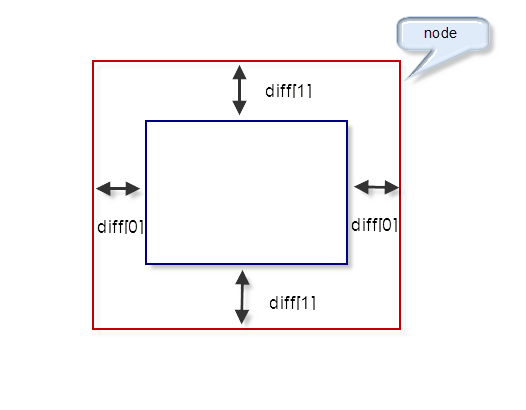
\includegraphics{scroll1.png}

\end{fulllineitems}



\end{description}\end{quote}

\end{fulllineitems}



\paragraph{实例方法}
\label{api/component/dd/scroll:id3}
\index{attach() (DD.Scroll method)}

\begin{fulllineitems}
\phantomsection\label{api/component/dd/scroll:DD.Scroll.attach}\pysiglinewithargsret{\code{Scroll.}\bfcode{attach}}{\emph{drag}}{}
注册可拖放对象到当前容器。
\begin{quote}\begin{description}
\item[{Parameters}] \leavevmode
\textbf{drag} (\emph{Draggable}) -- 需要使容器自动滚动的 Draggable 对象

\end{description}\end{quote}

\end{fulllineitems}


\index{unAttach() (DD.Scroll method)}

\begin{fulllineitems}
\phantomsection\label{api/component/dd/scroll:DD.Scroll.unAttach}\pysiglinewithargsret{\code{Scroll.}\bfcode{unAttach}}{\emph{drag}}{}
解除当前容器关联的可拖放对象。
\begin{quote}\begin{description}
\item[{Parameters}] \leavevmode
\textbf{drag} (\emph{Draggable}) -- 使容器自动滚动的 Draggable 对象

\end{description}\end{quote}

\end{fulllineitems}


\index{destroy() (DD.Scroll method)}

\begin{fulllineitems}
\phantomsection\label{api/component/dd/scroll:DD.Scroll.destroy}\pysiglinewithargsret{\code{Scroll.}\bfcode{destroy}}{}{}
解除当前容器关联的所有可拖放对象。

\end{fulllineitems}

\phantomsection\label{api/component/suggest/index:module-Suggest}
\index{Suggest (module)}

\subsection{Suggest}
\label{api/component/suggest/index:suggest}\label{api/component/suggest/index::doc}
作者: \href{mailto:lifesinger@gmail.com}{玉伯}
\begin{enumerate}
\item {}
提示补全基本功能

\item {}
完全跨域

\item {}
小巧精简,仅依赖 ks-core, 压缩后不超过 9k

\item {}
支持所有 A 级浏览器

\item {}
cache 功能

\item {}
支持键盘控制:上下选择及回车后直接提交,ESC 键关闭

\item {}
支持鼠标控制:鼠标选择和点击提交功能

\item {}
{[}DELAY{]} 支持匹配文字加亮

\item {}
{[}DELAY{]} 动画效果

\item {}
{[}DELAY{]} 在提示层中显示第一个搜索结果

\item {}
{[}DELAY{]} 整合本地表单的提示记录

\item {}
{[}DELAY{]} 关键词的模糊匹配提示功能

\end{enumerate}


\subsubsection{Suggest}
\label{api/component/suggest/suggest:suggest}\label{api/component/suggest/suggest::doc}

\paragraph{构造器}
\label{api/component/suggest/suggest:id1}
\index{KISSY.Suggest (class in Suggest)}

\begin{fulllineitems}
\phantomsection\label{api/component/suggest/suggest:Suggest.KISSY.Suggest}\pysiglinewithargsret{\strong{class }\code{KISSY.}\bfcode{Suggest}}{\emph{textInput}, \emph{dataSource}, \emph{config}}{}~\begin{quote}\begin{description}
\item[{Parameters}] \leavevmode\begin{itemize}
\item {}
\textbf{textInput} (\emph{String\textbar{}HTMLElement}) -- 输入框

\item {}
\textbf{dataSource} (\emph{String}) -- 数据源

\item {}
\textbf{config} (\emph{Object}) --
配置项

\index{containerCls (Suggest.KISSY.Suggest attribute)}

\begin{fulllineitems}
\phantomsection\label{api/component/suggest/suggest:Suggest.KISSY.Suggest.containerCls}\pysigline{\bfcode{containerCls}}{}~
\begin{DUlineblock}{0em}
\item[] 悬浮提示层的class
\item[] 默认为空
\end{DUlineblock}

\end{fulllineitems}


\index{containerWidth (Suggest.KISSY.Suggest attribute)}

\begin{fulllineitems}
\phantomsection\label{api/component/suggest/suggest:Suggest.KISSY.Suggest.containerWidth}\pysigline{\bfcode{containerWidth}}{}~
\begin{DUlineblock}{0em}
\item[] 提示层的宽度,示范取值:`200px', `10\%' 等,必须带单位
\item[] 默认为空,和input输入框的宽度保持一致
\end{DUlineblock}

\end{fulllineitems}



\end{itemize}

\end{description}\end{quote}

\end{fulllineitems}



\paragraph{对象属性}
\label{api/component/suggest/suggest:id2}

\paragraph{对象方法}
\label{api/component/suggest/suggest:id3}

\paragraph{触发事件}
\label{api/component/suggest/suggest:id4}

\paragraph{类属性}
\label{api/component/suggest/suggest:id5}

\paragraph{类方法}
\label{api/component/suggest/suggest:id6}\phantomsection\label{api/component/template/index:module-Template}
\index{Template (module)}

\subsection{Template}
\label{api/component/template/index::doc}\label{api/component/template/index:template}
by \href{mailto:wenhe@taobao.com}{文河}


\subsubsection{特性}
\label{api/component/template/index:id2}\begin{itemize}
\item {}
模板语法,从 \code{\{\{\#tagName\}\}} 开始,由 \code{\{\{/tagName\}\}} 结束(如果有结束标签的话).

\item {}
模板变量, \code{\{\{variable\}\}} .

\item {}
原生支持 if/elseif/else/each/! 四个标签.

\item {}
支持嵌套.

\item {}
容错和调试.

\item {}
性能还不赖.

\item {}
容易扩展.

\end{itemize}


\subsubsection{模板语法和范例}
\label{api/component/template/index:id3}

\paragraph{变量}
\label{api/component/template/index:id4}
变量支持JavaScript语法里的任何有返回值的语句,比如  \code{name} ,  \code{user.name} ,  \code{user{[}0{]}.name} , 甚至可以使用方法,  \code{KISSY.one('\#template').html()}


\subparagraph{语法}
\label{api/component/template/index:id5}
\begin{Verbatim}[commandchars=\\\{\}]
\PYG{p}{\PYGZob{}}\PYG{p}{\PYGZob{}}\PYG{n+nx}{Variable}\PYG{p}{\PYGZcb{}}\PYG{p}{\PYGZcb{}}
\end{Verbatim}


\subparagraph{范例}
\label{api/component/template/index:id6}
\begin{Verbatim}[commandchars=\\\{\}]
\PYG{n+nx}{KISSY}\PYG{p}{.}\PYG{n+nx}{Template}\PYG{p}{(}\PYG{l+s+s1}{'Hello, \PYGZob{}\PYGZob{}name\PYGZcb{}\PYGZcb{}.'}\PYG{p}{)}
    \PYG{p}{.}\PYG{n+nx}{render}\PYG{p}{(}\PYG{p}{\PYGZob{}}\PYG{n+nx}{name}\PYG{o}{:} \PYG{l+s+s1}{'Frank'}\PYG{p}{\PYGZcb{}}\PYG{p}{)}\PYG{p}{;}

\PYG{n+nx}{Hello}\PYG{p}{,} \PYG{n+nx}{Frank}\PYG{p}{.}

\PYG{n+nx}{KISSY}\PYG{p}{.}\PYG{n+nx}{Template}\PYG{p}{(}\PYG{l+s+s1}{'Hello, \PYGZob{}\PYGZob{}user.name\PYGZcb{}\PYGZcb{}.'}\PYG{p}{)}
    \PYG{p}{.}\PYG{n+nx}{render}\PYG{p}{(}\PYG{p}{\PYGZob{}}\PYG{n+nx}{user}\PYG{o}{:} \PYG{p}{\PYGZob{}}\PYG{n+nx}{name}\PYG{o}{:} \PYG{l+s+s1}{'Frank'}\PYG{p}{\PYGZcb{}}\PYG{p}{\PYGZcb{}}\PYG{p}{)}\PYG{p}{;}

\PYG{n+nx}{Hello}\PYG{p}{,} \PYG{n+nx}{Frank}\PYG{p}{.}
\end{Verbatim}


\paragraph{if 语句}
\label{api/component/template/index:if}

\subparagraph{语法}
\label{api/component/template/index:id7}
\begin{Verbatim}[commandchars=@\[\]]
{{@#if conditions}}
    BLOCK
{{/if}}
\end{Verbatim}


\subparagraph{范例}
\label{api/component/template/index:id8}
\begin{Verbatim}[commandchars=\\\{\}]
\PYG{n+nx}{KISSY}\PYG{p}{.}\PYG{n+nx}{Template}\PYG{p}{(}\PYG{l+s+s1}{'Hello, \PYGZob{}\PYGZob{}\#if show\PYGZcb{}\PYGZcb{}\PYGZob{}\PYGZob{}name\PYGZcb{}\PYGZcb{}\PYGZob{}\PYGZob{}/if\PYGZcb{}\PYGZcb{})'}\PYG{p}{)}
    \PYG{p}{.}\PYG{n+nx}{render}\PYG{p}{(}\PYG{p}{\PYGZob{}}\PYG{n+nx}{show}\PYG{o}{:} \PYG{k+kc}{true}\PYG{p}{,} \PYG{n+nx}{name}\PYG{o}{:} \PYG{l+s+s1}{'Frank'}\PYG{p}{\PYGZcb{}}\PYG{p}{)}\PYG{p}{;}

\PYG{n+nx}{Hello}\PYG{p}{,} \PYG{n+nx}{Frank}
\end{Verbatim}


\paragraph{else和elseif}
\label{api/component/template/index:elseelseif}

\subparagraph{语法}
\label{api/component/template/index:id9}
\begin{Verbatim}[commandchars=@\[\]]
{{@#if conditions}}
    BLOCK
{{@#elseif conditions}}
    ELSEIF BLOCK
{{@#else}}
    ELSE BLOCK
{{/if}}
\end{Verbatim}


\subparagraph{范例}
\label{api/component/template/index:id10}
\begin{Verbatim}[commandchars=\\\{\}]
\PYG{n+nx}{KISSY}\PYG{p}{.}\PYG{n+nx}{Template}\PYG{p}{(}\PYG{l+s+s1}{'Hello, \PYGZob{}\PYGZob{}\#if showName\PYGZcb{}\PYGZcb{}\PYGZob{}\PYGZob{}name\PYGZcb{}\PYGZcb{}.\PYGZob{}\PYGZob{}\#else\PYGZcb{}\PYGZcb{}\PYGZob{}\PYGZob{}nick\PYGZcb{}\PYGZcb{}\PYGZob{}\PYGZob{}/if\PYGZcb{}\PYGZcb{})'}\PYG{p}{)}
    \PYG{p}{.}\PYG{n+nx}{render}\PYG{p}{(}\PYG{p}{\PYGZob{}}\PYG{n+nx}{showName}\PYG{o}{:} \PYG{k+kc}{false}\PYG{p}{,} \PYG{n+nx}{name}\PYG{o}{:} \PYG{l+s+s1}{'Frank'}\PYG{p}{,} \PYG{n+nx}{nick}\PYG{o}{:} \PYG{l+s+s1}{'yyfrankyy'}\PYG{p}{\PYGZcb{}}\PYG{p}{)}\PYG{p}{;}

\PYG{n+nx}{Hello}\PYG{p}{,} \PYG{n+nx}{yyfrankyy}\PYG{p}{.}

\PYG{n+nx}{KISSY}\PYG{p}{.}\PYG{n+nx}{Template}\PYG{p}{(}\PYG{l+s+s1}{'Hello, \PYGZob{}\PYGZob{}\#if name\PYGZcb{}\PYGZcb{}\PYGZob{}\PYGZob{}name\PYGZcb{}\PYGZcb{}.\PYGZob{}\PYGZob{}\#elseif nick\PYGZcb{}\PYGZcb{}\PYGZob{}\PYGZob{}nick\PYGZcb{}\PYGZcb{}\PYGZob{}\PYGZob{}/if\PYGZcb{}\PYGZcb{})'}\PYG{p}{)}
    \PYG{p}{.}\PYG{n+nx}{render}\PYG{p}{(}\PYG{p}{\PYGZob{}}\PYG{n+nx}{name}\PYG{o}{:} \PYG{l+s+s1}{'Frank'}\PYG{p}{,} \PYG{n+nx}{nick}\PYG{o}{:} \PYG{l+s+s1}{'yyfrankyy'}\PYG{p}{\PYGZcb{}}\PYG{p}{)}\PYG{p}{;}

\PYG{n+nx}{Hello}\PYG{p}{,} \PYG{n+nx}{Frank}\PYG{p}{.}
\end{Verbatim}


\paragraph{each}
\label{api/component/template/index:each}
循环读取某个变量,直接调用 \code{KISSY.each} 方法进行遍历.


\subparagraph{语法}
\label{api/component/template/index:id11}
\begin{Verbatim}[commandchars=@\[\]]
{{@#each conditions as value index}}
    BLOCK
{{/each}}
\end{Verbatim}

注意 \code{as value index} 可选


\subparagraph{范例1(使用默认的循环参数)}
\label{api/component/template/index:id12}
\begin{Verbatim}[commandchars=@\[\]]
KISSY.Template('Hello, {{@#each users}}@textless[]b color="{{@_ks@_value.color}}"@textgreater[]{{@_ks@_value.user}}@textless[]/b@textgreater[]{{/each}})')
    .render({users: @PYGZlb[]{name: 'Frank', color: 'red'}, {name: 'yyfrankyy', color: 'green'@PYGZrb[]});

Hello, @textless[]b color="red"@textgreater[]Frank@textless[]/b@textgreater[]@textless[]b color="green"@textgreater[]yyfrankyy@textless[]/b@textgreater[]
\end{Verbatim}


\subparagraph{范例2(使用自定义参数,可选)}
\label{api/component/template/index:id13}
\begin{Verbatim}[commandchars=@\[\]]
KISSY.Template('Hello, {{@#each users as user}}@textless[]b color="{{user.color}}"@textgreater[]{{user.name}}@textless[]/b@textgreater[]{{/each}})')
    .render({users: @PYGZlb[]{name: 'Frank', color: 'red'}, {name: 'yyfrankyy', color: 'green'@PYGZrb[]});

Hello, @textless[]b color="red"@textgreater[]Frank@textless[]/b@textgreater[]@textless[]b color="green"@textgreater[]yyfrankyy@textless[]/b@textgreater[]

KISSY.Template('Hello, {{@#each users as user index}}@textless[]b color="{{user.color}}"@textgreater[]{{index}}:{{user.name}}@textless[]/b@textgreater[]{{/each}})')
    .render({users: @PYGZlb[]{name: 'Frank', color: 'red'}, {name: 'yyfrankyy', color: 'green'@PYGZrb[]});

Hello, @textless[]b color="red"@textgreater[]0:Frank@textless[]/b@textgreater[]@textless[]b color="green"@textgreater[]1:yyfrankyy@textless[]/b@textgreater[]
\end{Verbatim}


\subparagraph{范例3(嵌套使用)}
\label{api/component/template/index:id14}
\begin{Verbatim}[commandchars=@\[\]]
KISSY.Template('Hello, {{@#each users as user}}@textless[]b color="{{user.color}}"@textgreater[]{{@#each user.names as name}}{{name}}{{/each}}@textless[]/b@textgreater[]{{/each}})')
    .render({users: @PYGZlb[]{names: @PYGZlb[]'Frank', 'Wang'@PYGZrb[], color: 'red'}, {names: @PYGZlb[]'Frank', 'Xu'@PYGZrb[], color: 'green'@PYGZrb[]});

Hello, @textless[]b color="red"@textgreater[]FrankWang@textless[]/b@textgreater[]@textless[]b color="green"@textgreater[]FrankXu@textless[]/b@textgreater[]
\end{Verbatim}


\paragraph{单行注释}
\label{api/component/template/index:id15}

\subparagraph{语法}
\label{api/component/template/index:id16}
\begin{Verbatim}[commandchars=@\[\]]
{{@#! comments}}
\end{Verbatim}


\subparagraph{范例}
\label{api/component/template/index:id17}
\begin{Verbatim}[commandchars=\\\{\}]
\PYG{n+nx}{KISSY}\PYG{p}{.}\PYG{n+nx}{Template}\PYG{p}{(}\PYG{l+s+s1}{'Hello, \PYGZob{}\PYGZob{}\#! here you go.\PYGZcb{}\PYGZcb{}\PYGZob{}\PYGZob{}name\PYGZcb{}\PYGZcb{}.'}\PYG{p}{)}\PYG{p}{.}\PYG{n+nx}{render}\PYG{p}{(}\PYG{p}{\PYGZob{}}\PYG{n+nx}{name}\PYG{o}{:} \PYG{l+s+s1}{'Frank'}\PYG{p}{\PYGZcb{}}\PYG{p}{)}\PYG{p}{;}

\PYG{n+nx}{Hello}\PYG{p}{,} \PYG{n+nx}{Frank}\PYG{p}{.}
\end{Verbatim}


\paragraph{标签嵌套}
\label{api/component/template/index:id18}
理论上支持任意标签嵌套,如果标签有关闭字符,记得关闭=,=,嵌套标签形成多代码块嵌套,作用域与JavaScript的作用域一致.


\subparagraph{语法}
\label{api/component/template/index:id19}
\begin{Verbatim}[commandchars=@\[\]]
{{@#each object}}
    {{@#if condition}}
        BLOCK
    {{/if}}
{{/each}}
\end{Verbatim}


\subparagraph{范例}
\label{api/component/template/index:id20}
\begin{Verbatim}[commandchars=\\\{\}]
\PYG{n+nx}{KISSY}\PYG{p}{.}\PYG{n+nx}{Template}\PYG{p}{(}\PYG{l+s+s1}{'Hello, \PYGZob{}\PYGZob{}\#each users\PYGZcb{}\PYGZcb{}\PYGZob{}\PYGZob{}\#if \PYGZus{}ks\PYGZus{}value.show\PYGZcb{}\PYGZcb{}\PYGZob{}\PYGZob{}\PYGZus{}ks\PYGZus{}value.name\PYGZcb{}\PYGZcb{}\PYGZob{}\PYGZob{}/if\PYGZcb{}\PYGZcb{}\PYGZob{}\PYGZob{}/each\PYGZcb{}\PYGZcb{}.'}\PYG{p}{)}
    \PYG{p}{.}\PYG{n+nx}{render}\PYG{p}{(}\PYG{p}{\PYGZob{}}\PYG{n+nx}{users}\PYG{o}{:} \PYG{p}{[}\PYG{p}{\PYGZob{}}\PYG{n+nx}{show}\PYG{o}{:} \PYG{k+kc}{false}\PYG{p}{,} \PYG{n+nx}{name}\PYG{o}{:} \PYG{l+s+s1}{'Frank'}\PYG{p}{\PYGZcb{}}\PYG{p}{,} \PYG{p}{\PYGZob{}}\PYG{n+nx}{show}\PYG{o}{:} \PYG{k+kc}{true}\PYG{p}{,} \PYG{n+nx}{name}\PYG{o}{:} \PYG{l+s+s1}{'yyfrankyy'}\PYG{p}{\PYGZcb{}}\PYG{p}{]}\PYG{p}{\PYGZcb{}}\PYG{p}{)}\PYG{p}{;}

\PYG{n+nx}{Hello}\PYG{p}{,} \PYG{n+nx}{yyfrankyy}\PYG{p}{.}
\end{Verbatim}


\subsubsection{容错和调试.}
\label{api/component/template/index:id21}

\paragraph{容错}
\label{api/component/template/index:id22}
目前支持两种错误信息:
\begin{enumerate}
\item {}
Syntax Error. 指模板在预编译阶段发生语法错误(模板编译后生成的脚本语法错误).

\item {}
Render Error. 指模板在渲染时发生错误(运行时错误,数据错误,或者模板变量错误等).

\end{enumerate}


\paragraph{调试}
\label{api/component/template/index:id23}
默认情况下,模板将编译时和运行时的错误,直接返回到结果里.

调试过程可调用 \code{KISSY.Template.log()} 方法输出渲染方法,定位脚本模板错误,并可通过引用 \code{jsbeauty} 来格式化生成的模板方法.


\subsubsection{模板性能对比}
\label{api/component/template/index:id24}
\href{https://spreadsheets.google.com/ccc?key=0ApZFGfLktT7FdDgtcGdzWV9wSzRpX2FRTElzZmVoV2c\&hl=en\#gid=3}{https://spreadsheets.google.com/ccc?key=0ApZFGfLktT7FdDgtcGdzWV9wSzRpX2FRTElzZmVoV2c\&hl=en\#gid=3}


\subsubsection{扩展}
\label{api/component/template/index:id25}
模板方法仅依赖于KISSY的 \code{core} 部分,默认调用为:

\begin{Verbatim}[commandchars=\\\{\}]
\PYG{n+nx}{KISSY}\PYG{p}{.}\PYG{n+nx}{Template}\PYG{p}{(}\PYG{l+s+s1}{'template here.'}\PYG{p}{)}\PYG{p}{.}\PYG{n+nx}{render}\PYG{p}{(}\PYG{n+nx}{data}\PYG{p}{)}\PYG{p}{;}
\end{Verbatim}

而:

\begin{Verbatim}[commandchars=\\\{\}]
\PYG{k+kd}{var} \PYG{n+nx}{templ} \PYG{o}{=} \PYG{n+nx}{KISSY}\PYG{p}{.}\PYG{n+nx}{Template}\PYG{p}{(}\PYG{p}{)}\PYG{p}{;}
\end{Verbatim}

可直接预编译模板方法.


\paragraph{API}
\label{api/component/template/index:api}

\subparagraph{KISSY.tmpl}
\label{api/component/template/index:kissy-tmpl}
\begin{Verbatim}[commandchars=\\\{\}]
\PYG{n+nx}{KISSY}\PYG{p}{.}\PYG{n+nx}{tmpl}\PYG{p}{(}\PYG{l+s+s1}{'\#template'}\PYG{p}{,} \PYG{p}{\PYGZob{}}\PYG{n+nx}{name}\PYG{o}{:} \PYG{l+s+s1}{'Frank'}\PYG{p}{\PYGZcb{}}\PYG{p}{)}\PYG{p}{.}\PYG{n+nx}{appendTo}\PYG{p}{(}\PYG{l+s+s1}{'\#container'}\PYG{p}{)}\PYG{p}{;}
\end{Verbatim}


\paragraph{语法扩展}
\label{api/component/template/index:id26}\begin{quote}

\code{KISSY.Template.addStatement()} 方法,提供扩展语法的接口,目前支持标签语法开始,关闭及一个参数传递.
\end{quote}

比如:

\begin{Verbatim}[commandchars=\\\{\}]
\PYG{n+nx}{KISSY}\PYG{p}{.}\PYG{n+nx}{Template}\PYG{p}{.}\PYG{n+nx}{addStatement}\PYG{p}{(}\PYG{p}{\PYGZob{}}\PYG{l+s+s1}{'while'}\PYG{o}{:} \PYG{p}{\PYGZob{}}
    \PYG{n+nx}{start}\PYG{o}{:} \PYG{l+s+s1}{'while(KS\PYGZus{}TEMPL\PYGZus{}STAT\PYGZus{}PARAM)\PYGZob{}'}\PYG{p}{,}
    \PYG{n+nx}{end}\PYG{o}{:} \PYG{l+s+s1}{'\PYGZcb{}'}
\PYG{p}{\PYGZcb{}}\PYG{p}{\PYGZcb{}}\PYG{p}{)}\PYG{p}{;}
\end{Verbatim}

即可支持 \code{while} 语句

\begin{Verbatim}[commandchars=@\[\]]
{{@#while true}}
    BLOCK
{{/while}}
\end{Verbatim}


\chapter{范例}
\label{demo/index:demo}\label{demo/index::doc}\label{demo/index:id1}

\section{Seed}
\label{demo/seed/index:seed}\label{demo/seed/index::doc}

\subsection{Loader}
\label{demo/seed/loader/index::doc}\label{demo/seed/loader/index:loader}
by \href{mailto:yiminghe@gmail.com}{承玉}


\subsubsection{\textless{} 1.2}
\label{demo/seed/loader/index:id2}

\paragraph{注册模块}
\label{demo/seed/loader/index:id3}
\begin{Verbatim}[commandchars=\\\{\}]
\PYG{n+nx}{KISSY}\PYG{p}{.}\PYG{n+nx}{add}\PYG{p}{(}\PYG{p}{\PYGZob{}}
   \PYG{l+s+s2}{"1.1x-dep"}\PYG{o}{:}\PYG{p}{\PYGZob{}}
        \PYG{n+nx}{fullpath}\PYG{o}{:}\PYG{l+s+s2}{"http://lite-ext.googlecode.com/svn/trunk/lite-ext/playground/module\PYGZus{}package/1.1x/dep.js"}
   \PYG{p}{\PYGZcb{}}\PYG{p}{,}
   \PYG{l+s+s2}{"1.1x-mod"}\PYG{o}{:}\PYG{p}{\PYGZob{}}
        \PYG{n+nx}{fullpath}\PYG{o}{:}\PYG{l+s+s2}{"http://lite-ext.googlecode.com/svn/trunk/lite-ext/playground/module\PYGZus{}package/1.1x/mod.js"}\PYG{p}{,}
        \PYG{n+nx}{cssfullpath}\PYG{o}{:}\PYG{l+s+s2}{"http://lite-ext.googlecode.com/svn/trunk/lite-ext/playground/module\PYGZus{}package/1.1x/mod.css"}\PYG{p}{,}
        \PYG{n+nx}{requires}\PYG{o}{:}\PYG{p}{[}\PYG{l+s+s2}{"1.1x-dep"}\PYG{p}{]}
   \PYG{p}{\PYGZcb{}}
\PYG{p}{\PYGZcb{}}\PYG{p}{)}\PYG{p}{;}
\end{Verbatim}


\paragraph{定义模块}
\label{demo/seed/loader/index:id4}
\href{http://lite-ext.googlecode.com/svn/trunk/lite-ext/playground/module\_package/1.1x/dep.js}{被依赖模块 1.1x dep}

\begin{Verbatim}[commandchars=\\\{\}]
\PYG{n+nx}{KISSY}\PYG{p}{.}\PYG{n+nx}{add}\PYG{p}{(}\PYG{l+s+s2}{"1.1x-dep"}\PYG{p}{,}\PYG{k+kd}{function}\PYG{p}{(}\PYG{p}{)}\PYG{p}{\PYGZob{}}
    \PYG{n+nx}{alert}\PYG{p}{(}\PYG{l+s+s2}{"1.1x-dep loaded"}\PYG{p}{)}\PYG{p}{;}
\PYG{p}{\PYGZcb{}}\PYG{p}{)}\PYG{p}{;}
\end{Verbatim}

\href{http://lite-ext.googlecode.com/svn/trunk/lite-ext/playground/module\_package/1.1x/mod.js}{主模块 1.1x mod}

\begin{Verbatim}[commandchars=\\\{\}]
\PYG{n+nx}{KISSY}\PYG{p}{.}\PYG{n+nx}{add}\PYG{p}{(}\PYG{l+s+s2}{"1.1x-mod"}\PYG{p}{,}\PYG{k+kd}{function}\PYG{p}{(}\PYG{p}{)}\PYG{p}{\PYGZob{}}
    \PYG{n+nx}{alert}\PYG{p}{(}\PYG{l+s+s2}{"1.1x-mod loaded"}\PYG{p}{)}\PYG{p}{;}
\PYG{p}{\PYGZcb{}}\PYG{p}{)}\PYG{p}{;}
\end{Verbatim}


\paragraph{使用模块}
\label{demo/seed/loader/index:id5}
\begin{Verbatim}[commandchars=\\\{\}]
\PYG{n+nx}{KISSY}\PYG{p}{.}\PYG{n+nx}{use}\PYG{p}{(}\PYG{l+s+s2}{"1.1x-mod"}\PYG{p}{)}\PYG{p}{;}
\end{Verbatim}


\paragraph{demo}
\label{demo/seed/loader/index:demo}

\subsubsection{1.2}
\label{demo/seed/loader/index:id6}

\paragraph{包配置}
\label{demo/seed/loader/index:id7}
\begin{Verbatim}[commandchars=\\\{\}]
\PYG{n+nx}{KISSY}\PYG{p}{.}\PYG{n+nx}{config}\PYG{p}{(}\PYG{p}{\PYGZob{}}
    \PYG{n+nx}{packages}\PYG{o}{:}\PYG{p}{[}
        \PYG{p}{\PYGZob{}}
            \PYG{n+nx}{name}\PYG{o}{:}\PYG{l+s+s2}{"1.2"}\PYG{p}{,} \PYG{c+c1}{//包名}
            \PYG{n+nx}{tag}\PYG{o}{:}\PYG{l+s+s2}{"20110323"}\PYG{p}{,}\PYG{c+c1}{//时间戳,添加在动态脚本路径后面,用于更新包内模块代码}
            \PYG{n+nx}{path}\PYG{o}{:}\PYG{l+s+s2}{"http://lite-ext.googlecode.com/svn/trunk/lite-ext/playground/module\PYGZus{}package/"}\PYG{p}{,} \PYG{c+c1}{//包对应路径,相对路径指相对于当前页面路径}
            \PYG{n+nx}{charset}\PYG{o}{:}\PYG{l+s+s2}{"gbk"} \PYG{c+c1}{//包里模块文件编码格式}
        \PYG{p}{\PYGZcb{}}
    \PYG{p}{]}
\PYG{p}{\PYGZcb{}}\PYG{p}{)}\PYG{p}{;}
\end{Verbatim}


\paragraph{定义模块}
\label{demo/seed/loader/index:id8}
\href{http://lite-ext.googlecode.com/svn/trunk/lite-ext/playground/module\_package/1.2/dep.js}{被依赖模块 1.2 dep}

\begin{Verbatim}[commandchars=\\\{\}]
\PYG{n+nx}{KISSY}\PYG{p}{.}\PYG{n+nx}{add}\PYG{p}{(}\PYG{k+kd}{function}\PYG{p}{(}\PYG{p}{)}\PYG{p}{\PYGZob{}}
    \PYG{n+nx}{alert}\PYG{p}{(}\PYG{l+s+s2}{"1.2/dep loaded"}\PYG{p}{)}\PYG{p}{;}
\PYG{p}{\PYGZcb{}}\PYG{p}{)}\PYG{p}{;}
\end{Verbatim}

\href{http://lite-ext.googlecode.com/svn/trunk/lite-ext/playground/module\_package/1.2/mod.js}{主模块 1.2 mod}

\begin{Verbatim}[commandchars=\\\{\}]
\PYG{n+nx}{KISSY}\PYG{p}{.}\PYG{n+nx}{add}\PYG{p}{(}\PYG{k+kd}{function}\PYG{p}{(}\PYG{p}{)}\PYG{p}{\PYGZob{}}
    \PYG{n+nx}{alert}\PYG{p}{(}\PYG{l+s+s2}{"1.2/mod loaded"}\PYG{p}{)}\PYG{p}{;}
\PYG{p}{\PYGZcb{}}\PYG{p}{,}\PYG{p}{\PYGZob{}}
    \PYG{n+nx}{requires}\PYG{o}{:}\PYG{p}{[}\PYG{l+s+s2}{"./dep"}\PYG{p}{,}\PYG{l+s+s2}{"./mod.css"}\PYG{p}{]} \PYG{c+c1}{//相对于当前模块js 定位}
\PYG{p}{\PYGZcb{}}\PYG{p}{)}\PYG{p}{;}
\end{Verbatim}


\paragraph{使用模块}
\label{demo/seed/loader/index:id9}
\begin{Verbatim}[commandchars=\\\{\}]
\PYG{n+nx}{KISSY}\PYG{p}{.}\PYG{n+nx}{use}\PYG{p}{(}\PYG{l+s+s2}{"1.2/mod"}\PYG{p}{)}\PYG{p}{;}
\end{Verbatim}


\paragraph{demo}
\label{demo/seed/loader/index:id10}

\section{Core}
\label{demo/core/index:core}\label{demo/core/index::doc}

\subsection{Anim}
\label{demo/core/anim/index:anim}\label{demo/core/anim/index::doc}
by \href{mailto:yiminghe@gmail.com}{承玉}


\subsubsection{使用构造器}
\label{demo/core/anim/index:id2}
源码:

\begin{Verbatim}[commandchars=\\\{\}]
\PYG{n+nx}{KISSY}\PYG{p}{.}\PYG{n+nx}{use}\PYG{p}{(}\PYG{l+s+s2}{"anim,node"}\PYG{p}{,}\PYG{k+kd}{function}\PYG{p}{(}\PYG{n+nx}{S}\PYG{p}{,}\PYG{n+nx}{Anim}\PYG{p}{,}\PYG{n+nx}{Node}\PYG{p}{)}\PYG{p}{\PYGZob{}}
    \PYG{c+c1}{//KISSY 1.2 以前可通过 var Node=S.Node ; var Anim=S.Anim}
     \PYG{k+kd}{var} \PYG{n+nx}{anim} \PYG{o}{=} \PYG{n+nx}{Anim}\PYG{p}{(}
                \PYG{l+s+s1}{'\#test1'}\PYG{p}{,}
                \PYG{p}{\PYGZob{}}
                    \PYG{l+s+s1}{'background-color'}\PYG{o}{:}\PYG{l+s+s1}{'\#fcc'}\PYG{p}{,}
                    \PYG{c+c1}{//'border': '5px dashed \#999',}
                    \PYG{l+s+s1}{'border-wdith'}\PYG{o}{:}\PYG{l+s+s1}{'5px'}\PYG{p}{,}
                    \PYG{l+s+s1}{'border-color'}\PYG{o}{:}\PYG{l+s+s2}{"\#999999"}\PYG{p}{,}
                    \PYG{l+s+s1}{'border-style'}\PYG{o}{:}\PYG{l+s+s2}{"dashed"}\PYG{p}{,}
                    \PYG{l+s+s1}{'width'}\PYG{o}{:} \PYG{l+s+s1}{'100px'}\PYG{p}{,}
                    \PYG{l+s+s1}{'height'}\PYG{o}{:} \PYG{l+s+s1}{'50px'}\PYG{p}{,}
                    \PYG{l+s+s1}{'left'}\PYG{o}{:} \PYG{l+s+s1}{'900px'}\PYG{p}{,}
                    \PYG{l+s+s1}{'top'}\PYG{o}{:} \PYG{l+s+s1}{'285px'}\PYG{p}{,}
                    \PYG{l+s+s1}{'opacity'}\PYG{o}{:} \PYG{l+s+s1}{'.5'}\PYG{p}{,}
                    \PYG{l+s+s1}{'font-size'}\PYG{o}{:} \PYG{l+s+s1}{'48px'}\PYG{p}{,}
                    \PYG{l+s+s1}{'padding'}\PYG{o}{:} \PYG{l+s+s1}{'30px 0'}\PYG{p}{,}
                    \PYG{l+s+s1}{'color'}\PYG{o}{:} \PYG{l+s+s1}{'\#FF3333'}
                \PYG{p}{\PYGZcb{}}\PYG{p}{,}\PYG{l+m+mi}{5}\PYG{p}{,}
                \PYG{l+s+s1}{'bounceOut'}\PYG{p}{,}\PYG{k+kd}{function}\PYG{p}{(}\PYG{p}{)}\PYG{p}{\PYGZob{}}
                    \PYG{n+nx}{alert}\PYG{p}{(}\PYG{l+s+s1}{'demo1 结束'}\PYG{p}{)}\PYG{p}{;}
                \PYG{p}{\PYGZcb{}}\PYG{p}{)}\PYG{p}{;}
     \PYG{n+nx}{S}\PYG{p}{.}\PYG{n+nx}{one}\PYG{p}{(}\PYG{l+s+s2}{"\#test1-btn"}\PYG{p}{)}\PYG{p}{.}\PYG{n+nx}{on}\PYG{p}{(}\PYG{l+s+s2}{"click"}\PYG{p}{,}\PYG{k+kd}{function}\PYG{p}{(}\PYG{p}{)}\PYG{p}{\PYGZob{}}
        \PYG{n+nx}{anim}\PYG{p}{.}\PYG{n+nx}{run}\PYG{p}{(}\PYG{p}{)}\PYG{p}{;}
     \PYG{p}{\PYGZcb{}}\PYG{p}{)}\PYG{p}{;}
\PYG{p}{\PYGZcb{}}\PYG{p}{)}\PYG{p}{;}
\end{Verbatim}


\subsubsection{滚动属性动画实例}
\label{demo/core/anim/index:id3}
源码:

\begin{Verbatim}[commandchars=\\\{\}]
\PYG{n+nx}{KISSY}\PYG{p}{.}\PYG{n+nx}{use}\PYG{p}{(}\PYG{l+s+s2}{"anim"}\PYG{p}{,}\PYG{k+kd}{function}\PYG{p}{(}\PYG{n+nx}{S}\PYG{p}{,}\PYG{n+nx}{Anim}\PYG{p}{)}\PYG{p}{\PYGZob{}}
    \PYG{n+nx}{S}\PYG{p}{.}\PYG{n+nx}{one}\PYG{p}{(}\PYG{l+s+s2}{"\#test-scroll"}\PYG{p}{)}\PYG{p}{.}\PYG{n+nx}{on}\PYG{p}{(}\PYG{l+s+s2}{"click"}\PYG{p}{,} \PYG{k+kd}{function}\PYG{p}{(}\PYG{p}{)} \PYG{p}{\PYGZob{}}
        \PYG{n+nx}{S}\PYG{p}{.}\PYG{n+nx}{one}\PYG{p}{(}\PYG{l+s+s2}{"\#test-scroll"}\PYG{p}{)}\PYG{p}{[}\PYG{l+m+mi}{0}\PYG{p}{]}\PYG{p}{.}\PYG{n+nx}{disabled} \PYG{o}{=} \PYG{k+kc}{true}\PYG{p}{;}
        \PYG{n+nx}{Anim}\PYG{p}{(}\PYG{n+nx}{S}\PYG{p}{.}\PYG{n+nx}{get}\PYG{p}{(}\PYG{l+s+s2}{"\#test8"}\PYG{p}{)}\PYG{p}{,}\PYG{p}{\PYGZob{}}
            \PYG{c+c1}{//设置 scrollLeft 或者 scrollTop 属性}
            \PYG{n+nx}{scrollLeft}\PYG{o}{:}\PYG{l+m+mi}{500}
        \PYG{p}{\PYGZcb{}}\PYG{p}{,} \PYG{l+m+mi}{5}\PYG{p}{,} \PYG{k+kc}{undefined}\PYG{p}{,} \PYG{k+kd}{function}\PYG{p}{(}\PYG{p}{)} \PYG{p}{\PYGZob{}}
            \PYG{n+nx}{Anim}\PYG{p}{(}\PYG{n+nx}{S}\PYG{p}{.}\PYG{n+nx}{get}\PYG{p}{(}\PYG{l+s+s2}{"\#test8"}\PYG{p}{)}\PYG{p}{,}\PYG{p}{\PYGZob{}}
                \PYG{n+nx}{scrollLeft}\PYG{o}{:}\PYG{l+m+mi}{0}
            \PYG{p}{\PYGZcb{}}\PYG{p}{,} \PYG{l+m+mi}{5}\PYG{p}{,} \PYG{k+kc}{undefined}\PYG{p}{,} \PYG{k+kd}{function}\PYG{p}{(}\PYG{p}{)} \PYG{p}{\PYGZob{}}
                \PYG{n+nx}{S}\PYG{p}{.}\PYG{n+nx}{one}\PYG{p}{(}\PYG{l+s+s2}{"\#test-scroll"}\PYG{p}{)}\PYG{p}{[}\PYG{l+m+mi}{0}\PYG{p}{]}\PYG{p}{.}\PYG{n+nx}{disabled} \PYG{o}{=} \PYG{k+kc}{false}\PYG{p}{;}
            \PYG{p}{\PYGZcb{}}\PYG{p}{)}\PYG{p}{.}\PYG{n+nx}{run}\PYG{p}{(}\PYG{p}{)}\PYG{p}{;}
        \PYG{p}{\PYGZcb{}}\PYG{p}{)}\PYG{p}{.}\PYG{n+nx}{run}\PYG{p}{(}\PYG{p}{)}\PYG{p}{;}
    \PYG{p}{\PYGZcb{}}\PYG{p}{)}\PYG{p}{;}
\PYG{p}{\PYGZcb{}}\PYG{p}{)}\PYG{p}{;}
\end{Verbatim}


\subsubsection{节点实例动画操作}
\label{demo/core/anim/index:id4}
源码:

\begin{Verbatim}[commandchars=\\\{\}]
\PYG{n+nx}{KISSY}\PYG{p}{.}\PYG{n+nx}{use}\PYG{p}{(}\PYG{l+s+s2}{"anim,node"}\PYG{p}{,}\PYG{k+kd}{function}\PYG{p}{(}\PYG{n+nx}{S}\PYG{p}{,}\PYG{n+nx}{Anim}\PYG{p}{,}\PYG{n+nx}{Node}\PYG{p}{)}\PYG{p}{\PYGZob{}}
    \PYG{c+c1}{//KISSY 1.2 以前可通过 var Node=S.Node ; var Anim=S.Anim}
    \PYG{k+kd}{var} \PYG{n+nx}{demo\PYGZus{}show}\PYG{o}{=}\PYG{n+nx}{S}\PYG{p}{.}\PYG{n+nx}{one}\PYG{p}{(}\PYG{l+s+s2}{"\#demo\PYGZus{}show"}\PYG{p}{)}\PYG{p}{,}
    \PYG{n+nx}{demo\PYGZus{}slide}\PYG{o}{=}\PYG{n+nx}{S}\PYG{p}{.}\PYG{n+nx}{one}\PYG{p}{(}\PYG{l+s+s2}{"\#demo\PYGZus{}slide"}\PYG{p}{)}\PYG{p}{,}
    \PYG{n+nx}{demo\PYGZus{}fade}\PYG{o}{=}\PYG{n+nx}{S}\PYG{p}{.}\PYG{n+nx}{one}\PYG{p}{(}\PYG{l+s+s2}{"\#demo\PYGZus{}fade"}\PYG{p}{)}\PYG{p}{;}

    \PYG{k+kd}{var} \PYG{n+nx}{anim\PYGZus{}show}\PYG{o}{=}\PYG{n+nx}{S}\PYG{p}{.}\PYG{n+nx}{one}\PYG{p}{(}\PYG{l+s+s2}{"\#anim\PYGZus{}show"}\PYG{p}{)}\PYG{p}{,}
    \PYG{n+nx}{anim\PYGZus{}slide}\PYG{o}{=}\PYG{n+nx}{S}\PYG{p}{.}\PYG{n+nx}{one}\PYG{p}{(}\PYG{l+s+s2}{"\#anim\PYGZus{}slide"}\PYG{p}{)}\PYG{p}{,}
    \PYG{n+nx}{anim\PYGZus{}fade}\PYG{o}{=}\PYG{n+nx}{S}\PYG{p}{.}\PYG{n+nx}{one}\PYG{p}{(}\PYG{l+s+s2}{"\#anim\PYGZus{}fade"}\PYG{p}{)}\PYG{p}{;}

    \PYG{n+nx}{demo\PYGZus{}show}\PYG{p}{.}\PYG{n+nx}{on}\PYG{p}{(}\PYG{l+s+s2}{"click"}\PYG{p}{,}\PYG{k+kd}{function}\PYG{p}{(}\PYG{p}{)}\PYG{p}{\PYGZob{}}
        \PYG{k}{if}\PYG{p}{(}\PYG{n+nx}{anim\PYGZus{}show}\PYG{p}{.}\PYG{n+nx}{css}\PYG{p}{(}\PYG{l+s+s2}{"display"}\PYG{p}{)}\PYG{o}{===}\PYG{l+s+s2}{"none"}\PYG{p}{)}
        \PYG{n+nx}{anim\PYGZus{}show}\PYG{p}{.}\PYG{n+nx}{show}\PYG{p}{(}\PYG{l+m+mi}{1}\PYG{p}{)}\PYG{p}{;}
        \PYG{k}{else}
        \PYG{n+nx}{anim\PYGZus{}show}\PYG{p}{.}\PYG{n+nx}{hide}\PYG{p}{(}\PYG{l+m+mi}{1}\PYG{p}{)}\PYG{p}{;}
    \PYG{p}{\PYGZcb{}}\PYG{p}{)}\PYG{p}{;}

    \PYG{n+nx}{demo\PYGZus{}slide}\PYG{p}{.}\PYG{n+nx}{on}\PYG{p}{(}\PYG{l+s+s2}{"click"}\PYG{p}{,}\PYG{k+kd}{function}\PYG{p}{(}\PYG{p}{)}\PYG{p}{\PYGZob{}}
        \PYG{k}{if}\PYG{p}{(}\PYG{n+nx}{anim\PYGZus{}slide}\PYG{p}{.}\PYG{n+nx}{css}\PYG{p}{(}\PYG{l+s+s2}{"display"}\PYG{p}{)}\PYG{o}{===}\PYG{l+s+s2}{"none"}\PYG{p}{)}
        \PYG{n+nx}{anim\PYGZus{}slide}\PYG{p}{.}\PYG{n+nx}{slideDown}\PYG{p}{(}\PYG{p}{)}\PYG{p}{;}
        \PYG{k}{else}
        \PYG{n+nx}{anim\PYGZus{}slide}\PYG{p}{.}\PYG{n+nx}{slideUp}\PYG{p}{(}\PYG{p}{)}\PYG{p}{;}
    \PYG{p}{\PYGZcb{}}\PYG{p}{)}\PYG{p}{;}

    \PYG{n+nx}{demo\PYGZus{}fade}\PYG{p}{.}\PYG{n+nx}{on}\PYG{p}{(}\PYG{l+s+s2}{"click"}\PYG{p}{,}\PYG{k+kd}{function}\PYG{p}{(}\PYG{p}{)}\PYG{p}{\PYGZob{}}
        \PYG{k}{if}\PYG{p}{(}\PYG{n+nx}{anim\PYGZus{}fade}\PYG{p}{.}\PYG{n+nx}{css}\PYG{p}{(}\PYG{l+s+s2}{"display"}\PYG{p}{)}\PYG{o}{===}\PYG{l+s+s2}{"none"}\PYG{p}{)}
        \PYG{n+nx}{anim\PYGZus{}fade}\PYG{p}{.}\PYG{n+nx}{fadeIn}\PYG{p}{(}\PYG{p}{)}\PYG{p}{;}
        \PYG{k}{else}
        \PYG{n+nx}{anim\PYGZus{}fade}\PYG{p}{.}\PYG{n+nx}{fadeOut}\PYG{p}{(}\PYG{p}{)}\PYG{p}{;}
    \PYG{p}{\PYGZcb{}}\PYG{p}{)}\PYG{p}{;}
\PYG{p}{\PYGZcb{}}\PYG{p}{)}\PYG{p}{;}
\end{Verbatim}


\section{Component}
\label{demo/component/index:component}\label{demo/component/index::doc}\phantomsection\label{demo/component/datalazyload/index:module-DataLazyload}
\index{DataLazyload (module)}

\subsection{DataLazyload}
\label{demo/component/datalazyload/index:datalazyload}\label{demo/component/datalazyload/index::doc}

\subsubsection{基本使用}
\label{demo/component/datalazyload/index:id1}
最简单的调用方式

\begin{Verbatim}[commandchars=\\\{\}]
\PYG{n+nx}{KISSY}\PYG{p}{.}\PYG{n+nx}{use}\PYG{p}{(}\PYG{l+s+s1}{'datalazyload'}\PYG{p}{,} \PYG{k+kd}{function}\PYG{p}{(}\PYG{n+nx}{S}\PYG{p}{,} \PYG{n+nx}{DataLazyload}\PYG{p}{)} \PYG{p}{\PYGZob{}}
    \PYG{n+nx}{S}\PYG{p}{.}\PYG{n+nx}{ready}\PYG{p}{(}\PYG{k+kd}{function}\PYG{p}{(}\PYG{n+nx}{S}\PYG{p}{)} \PYG{p}{\PYGZob{}}
        \PYG{n+nx}{S}\PYG{p}{.}\PYG{n+nx}{DataLazyload}\PYG{p}{(} \PYG{p}{\PYGZob{}} \PYG{n+nx}{mod}\PYG{o}{:} \PYG{l+s+s1}{'auto'} \PYG{p}{\PYGZcb{}} \PYG{p}{)}\PYG{p}{;}
    \PYG{p}{\PYGZcb{}}\PYG{p}{)}\PYG{p}{;}
\PYG{p}{\PYGZcb{}}\PYG{p}{)}\PYG{p}{;}
\end{Verbatim}

这样, 页面加载时就会自动延迟所有图片的下载, 以及延迟特定 textarea 里的 html 渲染.


\subsubsection{自动模式}
\label{demo/component/datalazyload/index:id2}
使用自动模式时, 设置配置项中的 \code{mod} 为 `auto' , 如下:

\begin{Verbatim}[commandchars=\\\{\}]
\PYG{k+kd}{var} \PYG{n+nx}{dataLazyload} \PYG{o}{=}\PYG{n+nx}{DataLazyload}\PYG{p}{(}\PYG{p}{\PYGZob{}}
    \PYG{n+nx}{placeholder} \PYG{o}{:} \PYG{l+s+s2}{"占位.png"}
    \PYG{n+nx}{mod}\PYG{o}{:}\PYG{l+s+s1}{'auto'}
\PYG{p}{\PYGZcb{}}\PYG{p}{)}\PYG{p}{;}
\end{Verbatim}

页面上出现大量图片元素时,

\begin{Verbatim}[commandchars=\\\{\}]
\PYG{n+nt}{\textless{}img} \PYG{n+na}{src=}\PYG{l+s}{"xx.png"} \PYG{n+nt}{/\textgreater{}}
\end{Verbatim}

会把当前视窗外的 img 的 src 保存在自定义属性中, 并将 src 替换为 placeholder (不指定为空), 当滚动导致该图片出现在当前视窗时将 src 设置已经保存的真实值.


\subsubsection{手动模式}
\label{demo/component/datalazyload/index:id3}
采用手动模式时, 需要自行在输出页面时, 可以不设置 img 的 src 属性, 但是必须设置 img 的 \code{data-ks-lazyload} 自定义属性为真实图片地址,  如:

\begin{Verbatim}[commandchars=\\\{\}]
\PYG{n+nt}{\textless{}img} \PYG{n+na}{data-ks-lazyload=}\PYG{l+s}{"xx.jpg"} \PYG{n+nt}{/\textgreater{}}
\end{Verbatim}

当滚动导致该图片出现在当前视窗时会将 src 设置为真实地址.


\subsubsection{textarea 延迟加载}
\label{demo/component/datalazyload/index:textarea}
\begin{notice}{note}{Note:}
\textbf{这种情况下和模式的手动自动没关系!}
\end{notice}

将页面中需要延迟的 DOM 节点, 放在

\begin{Verbatim}[commandchars=@\[\]]
@textless[]textarea class='ks-datalazyload invisible'/@textgreater[]dom code@textless[]/textarea/@textgreater[]
\end{Verbatim}

里. 可以添加 hidden 等 class, 但建议用 invisible (visiblity:hidden), 并设定 height = `实际高度', 这样可以保证滚动时无缝连接.
当滚动导致该 textarea 出现在当前视窗时会将该 textarea 内的 html 添加到新生成的 div 中, 并用新生成的 div 替换该 textarea .

\textbf{另外注意:}
\begin{enumerate}
\item {}
延迟 callback 约定:dataLazyload.addCallback(el, fn) 表示当 el 即将出现时, 触发 fn.

\item {}
所有操作都是最多触发一次, 比如来回拖动滚动条时, 只有 el 第一次出现时会触发 fn 回调.

\end{enumerate}


\subsubsection{全部示例}
\label{demo/component/datalazyload/index:id4}\begin{itemize}
\item {}
\href{http://docs.kissyui.com/kissy/src/datalazyload/test.html}{manual 模式}

\item {}
\href{http://docs.kissyui.com/kissy/src/datalazyload/test-auto.html}{auto 模式}

\end{itemize}


\subsection{Overlay}
\label{demo/component/overlay/index::doc}\label{demo/component/overlay/index:overlay}
by \href{mailto:yiminghe@gmail.com}{承玉}


\subsubsection{从 markup 中构建 overlay}
\label{demo/component/overlay/index:markup-overlay}
最常见的场景,弹出层 html 已经在页面 html 中,前端要做的是适时将它显示出来,例如页面中存在以下 html :

\begin{Verbatim}[commandchars=\\\{\}]
\PYG{n+nt}{\textless{}style}\PYG{n+nt}{\textgreater{}}
    \PYG{n+nf}{\#popup1} \PYG{p}{\PYGZob{}}
        \PYG{k}{position}\PYG{o}{:}\PYG{k}{absolute}\PYG{p}{;}
        \PYG{k}{left}\PYG{o}{:-}\PYG{l+m}{9999px}\PYG{p}{;}
        \PYG{k}{top}\PYG{o}{:-}\PYG{l+m}{9999px}\PYG{p}{;}
    \PYG{p}{\PYGZcb{}}
\PYG{n+nt}{\textless{}/style\textgreater{}}

\PYG{n+nt}{\textless{}div} \PYG{n+na}{id=}\PYG{l+s}{'popup1'}\PYG{n+nt}{\textgreater{}}
    我是一些提示信息
\PYG{n+nt}{\textless{}/div\textgreater{}}

\PYG{n+nt}{\textless{}button} \PYG{n+na}{id=}\PYG{l+s}{"btn1"}\PYG{n+nt}{\textgreater{}}Show\PYG{n+nt}{\textless{}/button\textgreater{}}
\PYG{n+nt}{\textless{}button} \PYG{n+na}{id=}\PYG{l+s}{"btn2"}\PYG{n+nt}{\textgreater{}}Hide\PYG{n+nt}{\textless{}/button\textgreater{}}
\end{Verbatim}


\paragraph{代码分解}
\label{demo/component/overlay/index:id2}
\begin{Verbatim}[commandchars=\\\{\}]
\PYG{n+nt}{\textless{}style}\PYG{n+nt}{\textgreater{}}
    \PYG{n+nf}{\#popup1} \PYG{p}{\PYGZob{}}
        \PYG{k}{position}\PYG{o}{:}\PYG{k}{absolute}\PYG{p}{;}
        \PYG{k}{left}\PYG{o}{:-}\PYG{l+m}{9999px}\PYG{p}{;}
        \PYG{k}{top}\PYG{o}{:-}\PYG{l+m}{9999px}\PYG{p}{;}
    \PYG{p}{\PYGZcb{}}
\PYG{n+nt}{\textless{}/style\textgreater{}}
\end{Verbatim}

初始载入时,弹出层所在 div 是浮出在屏幕之外而隐藏的,当点击 Show 按钮时,该弹层对齐在 Hide 按钮旁边,当点击 Hide 按钮时,已经显示的弹层就隐藏了。


\subparagraph{获得 overlay 对象}
\label{demo/component/overlay/index:id3}
通过 srcNode 配置项配置从已存的 dom 节点来生成 {\hyperref[api/component/overlay/overlay:Overlay.Overlay]{\code{Overlay}}} 对象 :

\begin{Verbatim}[commandchars=\\\{\},numbers=left,firstnumber=1,stepnumber=1]
\PYG{n+nx}{KISSY}\PYG{p}{.}\PYG{n+nx}{use}\PYG{p}{(}\PYG{l+s+s2}{"overlay"}\PYG{p}{,}\PYG{k+kd}{function}\PYG{p}{(}\PYG{n+nx}{S}\PYG{p}{,}\PYG{n+nx}{Overlay}\PYG{p}{)}\PYG{p}{\PYGZob{}}
    \PYG{c+c1}{// 对于 kissy \textless{} 1.2 ,可使用 Overlay = S.Overlay; 获取构造器}

    \PYG{k+kd}{var} \PYG{n+nx}{popup} \PYG{o}{=} \PYG{k}{new} \PYG{n+nx}{Overlay}\PYG{p}{(}\PYG{p}{\PYGZob{}}
        \PYG{n+nx}{srcNode}\PYG{o}{:}\PYG{n+nx}{S}\PYG{p}{.}\PYG{n+nx}{one}\PYG{p}{(}\PYG{l+s+s2}{"\#popup1"}\PYG{p}{)}\PYG{p}{,} \PYG{c+c1}{// 配置已存在 dom 节点}
        \PYG{n+nx}{width}\PYG{o}{:} \PYG{l+m+mi}{300}\PYG{p}{,} \PYG{c+c1}{// 配置宽度}
        \PYG{n+nx}{height}\PYG{o}{:} \PYG{l+m+mi}{200}\PYG{p}{,}    \PYG{c+c1}{// 配置高度}
        \PYG{n+nx}{align}\PYG{o}{:} \PYG{p}{\PYGZob{}}    \PYG{c+c1}{// 配置对齐属性}
            \PYG{n+nx}{node}\PYG{o}{:} \PYG{l+s+s1}{'\#btn2'}\PYG{p}{,}
            \PYG{n+nx}{points}\PYG{o}{:} \PYG{p}{[}\PYG{l+s+s1}{'tr'}\PYG{p}{,} \PYG{l+s+s1}{'tl'}\PYG{p}{]}\PYG{p}{,}
            \PYG{n+nx}{offset}\PYG{o}{:} \PYG{p}{[}\PYG{l+m+mi}{50}\PYG{p}{,} \PYG{l+m+mi}{0}\PYG{p}{]}
        \PYG{p}{\PYGZcb{}}
    \PYG{p}{\PYGZcb{}}\PYG{p}{)}\PYG{p}{;}

\PYG{p}{\PYGZcb{}}\PYG{p}{)}\PYG{p}{;}
\end{Verbatim}

当点击 Show 按钮时会触发弹出层的显示,以及点击 Hide 按钮时会触发弹出层的隐藏。

\begin{Verbatim}[commandchars=\\\{\},numbers=left,firstnumber=1,stepnumber=1]
\PYG{n+nx}{S}\PYG{p}{.}\PYG{n+nx}{one}\PYG{p}{(}\PYG{l+s+s1}{'\#btn1'}\PYG{p}{)}\PYG{p}{.}\PYG{n+nx}{on}\PYG{p}{(}\PYG{l+s+s1}{'click'}\PYG{p}{,} \PYG{k+kd}{function}\PYG{p}{(}\PYG{p}{)} \PYG{p}{\PYGZob{}}
    \PYG{c+c1}{// 根据对齐属性,显示在 Hide 按钮旁}
    \PYG{n+nx}{popup}\PYG{p}{.}\PYG{n+nx}{show}\PYG{p}{(}\PYG{p}{)}\PYG{p}{;}
\PYG{p}{\PYGZcb{}}\PYG{p}{)}\PYG{p}{;}

\PYG{n+nx}{S}\PYG{p}{.}\PYG{n+nx}{one}\PYG{p}{(}\PYG{l+s+s1}{'\#btn2'}\PYG{p}{)}\PYG{p}{.}\PYG{n+nx}{on}\PYG{p}{(}\PYG{l+s+s1}{'click'}\PYG{p}{,} \PYG{k+kd}{function}\PYG{p}{(}\PYG{p}{)} \PYG{p}{\PYGZob{}}
    \PYG{c+c1}{// 隐藏弹出层}
    \PYG{n+nx}{popup}\PYG{p}{.}\PYG{n+nx}{hide}\PYG{p}{(}\PYG{p}{)}\PYG{p}{;}
\PYG{p}{\PYGZcb{}}\PYG{p}{)}\PYG{p}{;}
\end{Verbatim}


\paragraph{最终 demo}
\label{demo/component/overlay/index:demo}

\subsubsection{全新创建一个 Dialog}
\label{demo/component/overlay/index:dialog}
有时可能弹窗本身并没有在 html 中存在,而是由脚本完全生成的,这时就不需要 {\hyperref[api/component/overlay/overlay:Overlay.srcNode]{\code{srcNode}}} 配置了,直接配置相关属性后即可完全由脚本生成所需的 dom 节点。


\paragraph{生成 dialog 对象}
\label{demo/component/overlay/index:id4}
注意:要使得弹出对话框头部可拖动,需要 \code{use("dd")} 使用拖放模块:

\begin{Verbatim}[commandchars=\\\{\},numbers=left,firstnumber=1,stepnumber=1]
\PYG{n+nx}{KISSY}\PYG{p}{.}\PYG{n+nx}{use}\PYG{p}{(}\PYG{l+s+s2}{"overlay,dd"}\PYG{p}{,}\PYG{k+kd}{function}\PYG{p}{(}\PYG{n+nx}{S}\PYG{p}{,}\PYG{n+nx}{Overlay}\PYG{p}{)}\PYG{p}{\PYGZob{}}

    \PYG{c+c1}{// if kissy \textgreater{}= 1.2}
    \PYG{k+kd}{var} \PYG{n+nx}{Dialog}\PYG{o}{=}\PYG{n+nx}{Overlay}\PYG{p}{.}\PYG{n+nx}{Dialog}\PYG{p}{;}

    \PYG{c+c1}{// 所有 kissy 版本可用}
    \PYG{k+kd}{var} \PYG{n+nx}{Dialog}\PYG{o}{=}\PYG{n+nx}{S}\PYG{p}{.}\PYG{n+nx}{Dialog}\PYG{p}{;}

    \PYG{c+c1}{// 脚本完全生成 dialog 对象}
    \PYG{k+kd}{var} \PYG{n+nx}{dialog} \PYG{o}{=} \PYG{k}{new} \PYG{n+nx}{Dialog}\PYG{p}{(}\PYG{p}{\PYGZob{}}
        \PYG{n+nx}{width}\PYG{o}{:} \PYG{l+m+mi}{400}\PYG{p}{,}  \PYG{c+c1}{// 对话框宽度}
        \PYG{n+nx}{bodyStyle}\PYG{o}{:}\PYG{p}{\PYGZob{}}
            \PYG{n+nx}{height}\PYG{o}{:} \PYG{l+m+mi}{300} \PYG{c+c1}{// 对话框体的高度}
        \PYG{p}{\PYGZcb{}}\PYG{p}{,}
        \PYG{n+nx}{headerContent}\PYG{o}{:} \PYG{l+s+s1}{'this is title'}\PYG{p}{,} \PYG{c+c1}{// 对话框头信息 html}
        \PYG{n+nx}{footerContent}\PYG{o}{:} \PYG{l+s+s1}{'footer'}\PYG{p}{,}    \PYG{c+c1}{// 对话框底部信息 html}
        \PYG{n+nx}{bodyContent}\PYG{o}{:} \PYG{l+s+s1}{'content'}\PYG{p}{,} \PYG{c+c1}{// 对话框体信息 html}
        \PYG{n+nx}{mask}\PYG{o}{:} \PYG{k+kc}{true}\PYG{p}{,}  \PYG{c+c1}{//  有遮罩层}
        \PYG{n+nx}{draggable}\PYG{o}{:} \PYG{k+kc}{true} \PYG{c+c1}{// 允许头部可拖放}
    \PYG{p}{\PYGZcb{}}\PYG{p}{)}\PYG{p}{;}

\PYG{p}{\PYGZcb{}}\PYG{p}{)}\PYG{p}{;}
\end{Verbatim}


\paragraph{触发 dialog 对象显示}
\label{demo/component/overlay/index:id5}
当点击按钮时,首先调用 {\hyperref[api/component/overlay/overlay:Overlay.Overlay.render]{\code{render()}}} 渲染 {\hyperref[api/component/overlay/dialog:Overlay.Dialog]{\code{Dialog}}} 对象,使得 dialog 生成的 dom 节点加入到文档树中,再调用 {\hyperref[api/component/overlay/overlay:Overlay.Overlay.center]{\code{center()}}} 使得对话框位置在当前视窗中央,最后调用 {\hyperref[api/component/overlay/overlay:Overlay.Overlay.show]{\code{show()}}} 显示 dialog:

\begin{Verbatim}[commandchars=\\\{\},numbers=left,firstnumber=1,stepnumber=1]
\PYG{n+nx}{S}\PYG{p}{.}\PYG{n+nx}{one}\PYG{p}{(}\PYG{l+s+s2}{"\#btn4"}\PYG{p}{)}\PYG{p}{.}\PYG{n+nx}{on}\PYG{p}{(}\PYG{l+s+s2}{"click"}\PYG{p}{,} \PYG{k+kd}{function}\PYG{p}{(}\PYG{p}{)} \PYG{p}{\PYGZob{}}
    \PYG{n+nx}{dialog}\PYG{p}{.}\PYG{n+nx}{render}\PYG{p}{(}\PYG{p}{)}\PYG{p}{;}
    \PYG{n+nx}{dialog}\PYG{p}{.}\PYG{n+nx}{center}\PYG{p}{(}\PYG{p}{)}\PYG{p}{;}
    \PYG{n+nx}{dialog}\PYG{p}{.}\PYG{n+nx}{show}\PYG{p}{(}\PYG{p}{)}\PYG{p}{;}
\PYG{p}{\PYGZcb{}}\PYG{p}{)}\PYG{p}{;}
\end{Verbatim}


\paragraph{最终 demo}
\label{demo/component/overlay/index:id6}

\subsubsection{全部 demo}
\label{demo/component/overlay/index:id7}\begin{itemize}
\item {}
\href{http://kissyteam.github.com/kissy/src/overlay/demo/demo.html}{KISSY.Overlay 1.1.6}

\item {}
\href{http://yiminghe.github.com/kissy/src/overlay/demo/demo.html}{KISSY.Overlay 1.2.0}

\end{itemize}


\subsection{Switchable}
\label{demo/component/switchable/index::doc}\label{demo/component/switchable/index:switchable}
by \href{mailto:qiaohua@gmail.com}{乔花}


\subsubsection{常见使用方式}
\label{demo/component/switchable/index:id2}

\paragraph{组织 HTML 结构}
\label{demo/component/switchable/index:html}
通常情况下, Switchable 组件的 HTML 结构为外层一个容器元素,内部又分成 trigger 列表 和 panel 列表 两部分,trigger 列表可无, 如下的 HTML 结构最为常见:
\begin{quote}

\begin{Verbatim}[commandchars=\\\{\}]
\PYG{n+nt}{\textless{}div} \PYG{n+na}{id=}\PYG{l+s}{"J\PYGZus{}Slide"}\PYG{n+nt}{\textgreater{}}  \PYG{c}{\textless{}!--}\PYG{c}{ 容器元素 }\PYG{c}{--\textgreater{}}
    \PYG{n+nt}{\textless{}ul} \PYG{n+na}{class=}\PYG{l+s}{"ks-switchable-nav"}\PYG{n+nt}{\textgreater{}}  \PYG{c}{\textless{}!--}\PYG{c}{ 触发器列表 }\PYG{c}{--\textgreater{}}
        \PYG{n+nt}{\textless{}li} \PYG{n+na}{class=}\PYG{l+s}{"ks-active"}\PYG{n+nt}{\textgreater{}}标题 A\PYG{n+nt}{\textless{}/li\textgreater{}}
        \PYG{n+nt}{\textless{}li}\PYG{n+nt}{\textgreater{}}标题 B\PYG{n+nt}{\textless{}/li\textgreater{}}
        \PYG{n+nt}{\textless{}li}\PYG{n+nt}{\textgreater{}}标题 C\PYG{n+nt}{\textless{}/li\textgreater{}}
        \PYG{n+nt}{\textless{}li}\PYG{n+nt}{\textgreater{}}标题 D\PYG{n+nt}{\textless{}/li\textgreater{}}
    \PYG{n+nt}{\textless{}/ul\textgreater{}}
    \PYG{n+nt}{\textless{}div} \PYG{n+na}{class=}\PYG{l+s}{"ks-switchable-content"}\PYG{n+nt}{\textgreater{}}  \PYG{c}{\textless{}!--}\PYG{c}{ 面板列表 }\PYG{c}{--\textgreater{}}
        \PYG{n+nt}{\textless{}div}\PYG{n+nt}{\textgreater{}}内容 A\PYG{n+nt}{\textless{}/div\textgreater{}}
        \PYG{n+nt}{\textless{}div} \PYG{n+na}{style=}\PYG{l+s}{"display: none"}\PYG{n+nt}{\textgreater{}}内容 B\PYG{n+nt}{\textless{}/div\textgreater{}}
        \PYG{n+nt}{\textless{}div} \PYG{n+na}{style=}\PYG{l+s}{"display: none"}\PYG{n+nt}{\textgreater{}}内容 C\PYG{n+nt}{\textless{}/div\textgreater{}}
        \PYG{n+nt}{\textless{}div} \PYG{n+na}{style=}\PYG{l+s}{"display: none"}\PYG{n+nt}{\textgreater{}}内容 D\PYG{n+nt}{\textless{}/div\textgreater{}}
    \PYG{n+nt}{\textless{}/div\textgreater{}}
\PYG{n+nt}{\textless{}/div\textgreater{}}
\end{Verbatim}
\end{quote}

但注意: 这种结构并不固定, 且有时需要根据不同组件, 不同需求修改结构并定义它们的样式;


\paragraph{JS 初始化}
\label{demo/component/switchable/index:js}
通过容器元素的 id 和相关配置, 构建 {\hyperref[api/component/switchable/switchable:Switchable.Switchable]{\code{Switchable}}} 对象 :

\begin{Verbatim}[commandchars=\\\{\},numbers=left,firstnumber=1,stepnumber=1]
\PYG{n+nx}{KISSY}\PYG{p}{.}\PYG{n+nx}{use}\PYG{p}{(}\PYG{l+s+s2}{"switchable"}\PYG{p}{,}\PYG{k+kd}{function}\PYG{p}{(}\PYG{n+nx}{S}\PYG{p}{,}\PYG{n+nx}{Switchable}\PYG{p}{)}\PYG{p}{\PYGZob{}}
    \PYG{c+c1}{// 对于 kissy \textless{} 1.2 ,可使用 Switchable = S.Switchable; 获取构造器}

    \PYG{k+kd}{var} \PYG{n+nx}{s} \PYG{o}{=} \PYG{k}{new} \PYG{n+nx}{Switchable}\PYG{p}{.}\PYG{n+nx}{Slide}\PYG{p}{(}\PYG{l+s+s1}{'\#J\PYGZus{}Slide'}\PYG{p}{,} \PYG{p}{\PYGZob{}}
        \PYG{n+nx}{effect}\PYG{o}{:} \PYG{l+s+s1}{'scrolly'}\PYG{p}{,}
        \PYG{n+nx}{easing}\PYG{o}{:} \PYG{l+s+s1}{'easeOutStrong'}\PYG{p}{,}
        \PYG{n+nx}{countdown}\PYG{o}{:} \PYG{k+kc}{true}\PYG{p}{,}
        \PYG{n+nx}{countdownFromStyle}\PYG{o}{:} \PYG{l+s+s1}{'width:18px'}
    \PYG{p}{\PYGZcb{}}\PYG{p}{)}\PYG{p}{;}
\PYG{p}{\PYGZcb{}}\PYG{p}{)}\PYG{p}{;}
\end{Verbatim}


\paragraph{最终 demo}
\label{demo/component/switchable/index:demo}

\subsubsection{全部示例}
\label{demo/component/switchable/index:id3}

\paragraph{Tabs}
\label{demo/component/switchable/index:tabs}\begin{itemize}
\item {}
\href{http://yiminghe.github.com/kissy/src/switchable/demo/tabs.html}{普通标签页}

\end{itemize}


\paragraph{Slide}
\label{demo/component/switchable/index:slide}\begin{itemize}
\item {}
\href{http://yiminghe.github.com/kissy/src/switchable/demo/slide.html\#demo2}{淘宝首页卡盘}

\item {}
\href{http://yiminghe.github.com/kissy/src/switchable/demo/slide.html\#demo3}{有啊首页开盘}

\item {}
\href{http://yiminghe.github.com/kissy/src/switchable/demo/slide.html\#demo5}{有啊滚动新闻条}

\item {}
\href{http://yiminghe.github.com/kissy/src/switchable/demo/slide.html\#slideFocus}{土豆今日焦点}

\end{itemize}


\paragraph{Carousel}
\label{demo/component/switchable/index:carousel}\begin{itemize}
\item {}
\href{http://yiminghe.github.com/kissy/src/switchable/demo/carousel.html\#demo4}{普通旋转木马}

\item {}
\href{http://yiminghe.github.com/kissy/src/switchable/demo/carousel.html\#J\_TinySlide}{类似于首页上的旋转木马}

\end{itemize}


\paragraph{Accordion}
\label{demo/component/switchable/index:accordion}\begin{itemize}
\item {}
\href{http://yiminghe.github.com/kissy/src/switchable/demo/accordion.html}{普通手风琴}

\end{itemize}


\subsection{DD}
\label{demo/component/dd/index:dd}\label{demo/component/dd/index::doc}
by \href{mailto:yiminghe@gmail.com}{承玉}


\subsubsection{Draggable \& Proxy}
\label{demo/component/dd/draggable-usage::doc}\label{demo/component/dd/draggable-usage:draggable-proxy}

\paragraph{引入}
\label{demo/component/dd/draggable-usage:id1}
页面引入 kissy.js :

\begin{Verbatim}[commandchars=\\\{\}]
\PYG{n+nt}{\textless{}script }\PYG{n+na}{src=}\PYG{l+s}{'kissy.js'}\PYG{n+nt}{\textgreater{}}\PYG{n+nt}{\textless{}/script\textgreater{}}
\end{Verbatim}
New in version 1.2: 通过 use 加载 dd 模块:
\begin{Verbatim}[commandchars=\\\{\}]
\PYG{n+nx}{KISSY}\PYG{p}{.}\PYG{n+nx}{use}\PYG{p}{(}\PYG{l+s+s2}{"dd"}\PYG{p}{,}\PYG{k+kd}{function}\PYG{p}{(}\PYG{n+nx}{S}\PYG{p}{,}\PYG{n+nx}{DD}\PYG{p}{)}\PYG{p}{\PYGZob{}}
    \PYG{k+kd}{var} \PYG{n+nx}{Draggable} \PYG{o}{=} \PYG{n+nx}{DD}\PYG{p}{.}\PYG{n+nx}{Draggable}\PYG{p}{;}
\PYG{p}{\PYGZcb{}}\PYG{p}{)}\PYG{p}{;}
\end{Verbatim}


\strong{See Also:}


KISSY 1.2 {\hyperref[api/seed/loader/index:module-Loader]{\code{Loader}}} 新增功能




\paragraph{demo}
\label{demo/component/dd/draggable-usage:draggable-usage-demo}\label{demo/component/dd/draggable-usage:demo}

\paragraph{分解}
\label{demo/component/dd/draggable-usage:id2}

\subparagraph{准备节点}
\label{demo/component/dd/draggable-usage:id3}
\begin{Verbatim}[commandchars=\\\{\}]
\PYG{n+nt}{\textless{}div} \PYG{n+na}{id=}\PYG{l+s}{'test-drag'} \PYG{n+na}{style=}\PYG{l+s}{'border:1px solid red;}
\PYG{l+s}{                    background:blue;width:100px;}
\PYG{l+s}{                    height:100px;color:white;'}\PYG{n+nt}{\textgreater{}}
  drag me
\PYG{n+nt}{\textless{}/div\textgreater{}}
\end{Verbatim}

设置代理节点样式

\begin{Verbatim}[commandchars=\\\{\}]
.ks-dd-proxy \PYGZob{}
    opacity:0.2;
    *filter:alpha(opacity=20);
\PYGZcb{}
\end{Verbatim}


\subparagraph{载入 dd 模块}
\label{demo/component/dd/draggable-usage:dd}
\begin{Verbatim}[commandchars=\\\{\}]
\PYG{n+nx}{KISSY}\PYG{p}{.}\PYG{n+nx}{use}\PYG{p}{(}\PYG{l+s+s2}{"dd"}\PYG{p}{,}\PYG{k+kd}{function}\PYG{p}{(}\PYG{n+nx}{S}\PYG{p}{,}\PYG{n+nx}{DD}\PYG{p}{)}\PYG{p}{\PYGZob{}}

\PYG{p}{\PYGZcb{}}\PYG{p}{)}\PYG{p}{;}
\end{Verbatim}


\subparagraph{初始化 draggable 对象}
\label{demo/component/dd/draggable-usage:draggable}
\begin{Verbatim}[commandchars=\\\{\}]
\PYG{k+kd}{var} \PYG{n+nx}{drag}\PYG{o}{=}\PYG{k}{new} \PYG{n+nx}{DD}\PYG{p}{.}\PYG{n+nx}{Draggable}\PYG{p}{(}\PYG{p}{\PYGZob{}}
    \PYG{n+nx}{node}\PYG{o}{:}\PYG{l+s+s1}{'\#test-drag'}\PYG{p}{,}
    \PYG{n+nx}{cursor}\PYG{o}{:}\PYG{l+s+s1}{'move'}
\PYG{p}{\PYGZcb{}}\PYG{p}{)}\PYG{p}{;}
\end{Verbatim}


\subparagraph{初始化 proxy 对象}
\label{demo/component/dd/draggable-usage:proxy}
然后 proxy 对象和 draggable 绑定

\begin{Verbatim}[commandchars=\\\{\}]
\PYG{k}{new} \PYG{n+nx}{Proxy}\PYG{p}{(}\PYG{p}{)}\PYG{p}{.}\PYG{n+nx}{attach}\PYG{p}{(}\PYG{n+nx}{drag}\PYG{p}{)}\PYG{p}{;}
\end{Verbatim}


\subparagraph{监控事件,处理移动}
\label{demo/component/dd/draggable-usage:id4}
\begin{Verbatim}[commandchars=\\\{\}]
\PYG{n+nx}{drag}\PYG{p}{.}\PYG{n+nx}{on}\PYG{p}{(}\PYG{l+s+s2}{"drag"}\PYG{p}{,}\PYG{k+kd}{function}\PYG{p}{(}\PYG{n+nx}{ev}\PYG{p}{)}\PYG{p}{\PYGZob{}}
    \PYG{n+nx}{drag}\PYG{p}{.}\PYG{n+nx}{get}\PYG{p}{(}\PYG{l+s+s2}{"node"}\PYG{p}{)}\PYG{p}{.}\PYG{n+nx}{offset}\PYG{p}{(}\PYG{p}{\PYGZob{}}
        \PYG{n+nx}{left}\PYG{o}{:}\PYG{n+nx}{ev}\PYG{p}{.}\PYG{n+nx}{left}\PYG{p}{,}
        \PYG{n+nx}{top}\PYG{o}{:}\PYG{n+nx}{ev}\PYG{p}{.}\PYG{n+nx}{top}
    \PYG{p}{\PYGZcb{}}\PYG{p}{)}\PYG{p}{;}
\PYG{p}{\PYGZcb{}}\PYG{p}{)}\PYG{p}{;}
\end{Verbatim}


\subsubsection{Droppable}
\label{demo/component/dd/droppable-usage:droppable}\label{demo/component/dd/droppable-usage::doc}

\paragraph{引入}
\label{demo/component/dd/droppable-usage:id1}
页面引入 kissy.js :

\begin{Verbatim}[commandchars=\\\{\}]
\PYG{n+nt}{\textless{}script }\PYG{n+na}{src=}\PYG{l+s}{'kissy.js'}\PYG{n+nt}{\textgreater{}}\PYG{n+nt}{\textless{}/script\textgreater{}}
\end{Verbatim}
New in version 1.2: 通过 use 加载 dd 模块:
\begin{Verbatim}[commandchars=\\\{\}]
\PYG{n+nx}{KISSY}\PYG{p}{.}\PYG{n+nx}{use}\PYG{p}{(}\PYG{l+s+s2}{"dd"}\PYG{p}{,}\PYG{k+kd}{function}\PYG{p}{(}\PYG{n+nx}{S}\PYG{p}{,}\PYG{n+nx}{DD}\PYG{p}{)}\PYG{p}{\PYGZob{}}
    \PYG{k+kd}{var} \PYG{n+nx}{Droppable} \PYG{o}{=} \PYG{n+nx}{DD}\PYG{p}{.}\PYG{n+nx}{Droppable}\PYG{p}{;}
\PYG{p}{\PYGZcb{}}\PYG{p}{)}\PYG{p}{;}
\end{Verbatim}


\strong{See Also:}


KISSY 1.2 {\hyperref[api/seed/loader/index:module-Loader]{\code{Loader}}} 新增功能




\paragraph{demo}
\label{demo/component/dd/droppable-usage:demo}

\paragraph{分解}
\label{demo/component/dd/droppable-usage:id2}

\subparagraph{准备节点}
\label{demo/component/dd/droppable-usage:id3}
\begin{Verbatim}[commandchars=\\\{\}]
\PYG{n+nt}{\textless{}div} \PYG{n+na}{id=}\PYG{l+s}{"container"} \PYG{n+na}{class=}\PYG{l+s}{"container"}\PYG{n+nt}{\textgreater{}}
    \PYG{n+nt}{\textless{}div} \PYG{n+na}{id=}\PYG{l+s}{"c1"} \PYG{n+na}{class=}\PYG{l+s}{"component"}\PYG{n+nt}{\textgreater{}}
        intersect drag
    \PYG{n+nt}{\textless{}/div\textgreater{}}

    \PYG{n+nt}{\textless{}div} \PYG{n+na}{id=}\PYG{l+s}{"c2"} \PYG{n+na}{class=}\PYG{l+s}{"component"}\PYG{n+nt}{\textgreater{}}
        point drag
    \PYG{n+nt}{\textless{}/div\textgreater{}}

    \PYG{n+nt}{\textless{}div} \PYG{n+na}{id=}\PYG{l+s}{"c3"} \PYG{n+na}{class=}\PYG{l+s}{"component"}\PYG{n+nt}{\textgreater{}}
        strict drag
    \PYG{n+nt}{\textless{}/div\textgreater{}}

    \PYG{n+nt}{\textless{}div} \PYG{n+na}{id=}\PYG{l+s}{"drop"}\PYG{n+nt}{\textgreater{}}
        drop zone
    \PYG{n+nt}{\textless{}/div\textgreater{}}
\PYG{n+nt}{\textless{}/div\textgreater{}}
\end{Verbatim}


\subparagraph{获取模块定义}
\label{demo/component/dd/droppable-usage:id4}
\begin{Verbatim}[commandchars=\\\{\}]
\PYG{n+nx}{KISSY}\PYG{p}{.}\PYG{n+nx}{use}\PYG{p}{(}\PYG{l+s+s2}{"node,dd"}\PYG{p}{,} \PYG{k+kd}{function} \PYG{p}{(}\PYG{n+nx}{S}\PYG{p}{,} \PYG{n+nx}{Node}\PYG{p}{,} \PYG{n+nx}{DD}\PYG{p}{)} \PYG{p}{\PYGZob{}}
    \PYG{k+kd}{var} \PYG{n+nx}{DDM} \PYG{o}{=} \PYG{n+nx}{DD}\PYG{p}{.}\PYG{n+nx}{DDM}\PYG{p}{,}
        \PYG{n+nx}{Draggable} \PYG{o}{=} \PYG{n+nx}{DD}\PYG{p}{.}\PYG{n+nx}{Draggable}\PYG{p}{,}
        \PYG{n+nx}{Droppable} \PYG{o}{=} \PYG{n+nx}{DD}\PYG{p}{.}\PYG{n+nx}{Droppable}\PYG{p}{;}
\PYG{p}{\PYGZcb{}}\PYG{p}{)}\PYG{p}{;}
\end{Verbatim}


\subparagraph{全局监控}
\label{demo/component/dd/droppable-usage:id5}
开始拖放前保存节点的定位信息:

\begin{Verbatim}[commandchars=\\\{\}]
\PYG{n+nx}{DDM}\PYG{p}{.}\PYG{n+nx}{on}\PYG{p}{(}\PYG{l+s+s2}{"dragstart"}\PYG{p}{,} \PYG{k+kd}{function}\PYG{p}{(}\PYG{n+nx}{ev}\PYG{p}{)} \PYG{p}{\PYGZob{}}
    \PYG{k+kd}{var} \PYG{n+nx}{c} \PYG{o}{=} \PYG{n+nx}{ev}\PYG{p}{.}\PYG{n+nx}{drag}\PYG{p}{;}
    \PYG{n+nx}{p} \PYG{o}{=} \PYG{n+nx}{c}\PYG{p}{.}\PYG{n+nx}{get}\PYG{p}{(}\PYG{l+s+s2}{"dragNode"}\PYG{p}{)}\PYG{p}{.}\PYG{n+nx}{css}\PYG{p}{(}\PYG{l+s+s2}{"position"}\PYG{p}{)}\PYG{p}{;}
\PYG{p}{\PYGZcb{}}\PYG{p}{)}\PYG{p}{;}
\end{Verbatim}

拖放中,根据位置信息设置节点坐标

\begin{Verbatim}[commandchars=\\\{\}]
\PYG{n+nx}{DDM}\PYG{p}{.}\PYG{n+nx}{on}\PYG{p}{(}\PYG{l+s+s2}{"drag"}\PYG{p}{,} \PYG{k+kd}{function}\PYG{p}{(}\PYG{n+nx}{ev}\PYG{p}{)} \PYG{p}{\PYGZob{}}
    \PYG{k+kd}{var} \PYG{n+nx}{c} \PYG{o}{=} \PYG{n+nx}{ev}\PYG{p}{.}\PYG{n+nx}{drag}\PYG{p}{;}
    \PYG{c+cm}{/**}
\PYG{c+cm}{     * node 和 dragNode 区别:}
\PYG{c+cm}{     * node : 可能是 proxy node,指实际拖放节点}
\PYG{c+cm}{     */}
    \PYG{n+nx}{c}\PYG{p}{.}\PYG{n+nx}{get}\PYG{p}{(}\PYG{l+s+s2}{"node"}\PYG{p}{)}\PYG{p}{.}\PYG{n+nx}{offset}\PYG{p}{(}\PYG{n+nx}{ev}\PYG{p}{)}\PYG{p}{;}
\PYG{p}{\PYGZcb{}}\PYG{p}{)}\PYG{p}{;}
\end{Verbatim}

拖放结束后,恢复节点的定位信息

\begin{Verbatim}[commandchars=\\\{\}]
\PYG{n+nx}{DDM}\PYG{p}{.}\PYG{n+nx}{on}\PYG{p}{(}\PYG{l+s+s2}{"dragend"}\PYG{p}{,} \PYG{k+kd}{function}\PYG{p}{(}\PYG{n+nx}{ev}\PYG{p}{)} \PYG{p}{\PYGZob{}}
    \PYG{k+kd}{var} \PYG{n+nx}{c} \PYG{o}{=} \PYG{n+nx}{ev}\PYG{p}{.}\PYG{n+nx}{drag}\PYG{p}{;}
    \PYG{n+nx}{c}\PYG{p}{.}\PYG{n+nx}{get}\PYG{p}{(}\PYG{l+s+s2}{"dragNode"}\PYG{p}{)}\PYG{p}{.}\PYG{n+nx}{css}\PYG{p}{(}\PYG{l+s+s2}{"position"}\PYG{p}{,} \PYG{n+nx}{p}\PYG{p}{)}\PYG{p}{;}
\PYG{p}{\PYGZcb{}}\PYG{p}{)}\PYG{p}{;}
\end{Verbatim}


\subparagraph{初始拖放对象}
\label{demo/component/dd/droppable-usage:id6}
实例化 3 个普通的拖实例以及一个放实例

\begin{Verbatim}[commandchars=\\\{\}]
\PYG{k+kd}{var} \PYG{n+nx}{c1} \PYG{o}{=} \PYG{k}{new} \PYG{n+nx}{Draggable}\PYG{p}{(}\PYG{p}{\PYGZob{}}
    \PYG{n+nx}{node}\PYG{o}{:}\PYG{l+s+s2}{"\#c1"}\PYG{p}{,}
    \PYG{c+c1}{//模式,}
    \PYG{c+c1}{// intersect :区域相交就算enter}
    \PYG{c+c1}{// strict : drag 区域完全在 drop 区域内才算}
    \PYG{c+c1}{// point : 鼠标在 drop 区域内}
    \PYG{c+c1}{//默认 point}
    \PYG{n+nx}{mode}\PYG{o}{:}\PYG{n+nx}{Draggable}\PYG{p}{.}\PYG{n+nx}{INTERSECT}
\PYG{p}{\PYGZcb{}}\PYG{p}{)}\PYG{p}{;}


\PYG{k+kd}{var} \PYG{n+nx}{c3} \PYG{o}{=} \PYG{k}{new} \PYG{n+nx}{Draggable}\PYG{p}{(}\PYG{p}{\PYGZob{}}
    \PYG{n+nx}{node}\PYG{o}{:}\PYG{l+s+s2}{"\#c3"}\PYG{p}{,}
    \PYG{n+nx}{mode}\PYG{o}{:}\PYG{n+nx}{Draggable}\PYG{p}{.}\PYG{n+nx}{STRICT}
\PYG{p}{\PYGZcb{}}\PYG{p}{)}\PYG{p}{;}


\PYG{k+kd}{var} \PYG{n+nx}{c2} \PYG{o}{=} \PYG{k}{new} \PYG{n+nx}{Draggable}\PYG{p}{(}\PYG{p}{\PYGZob{}}
    \PYG{n+nx}{node}\PYG{o}{:}\PYG{l+s+s2}{"\#c2"}
\PYG{p}{\PYGZcb{}}\PYG{p}{)}\PYG{p}{;}


\PYG{k+kd}{var} \PYG{n+nx}{drop} \PYG{o}{=} \PYG{k}{new} \PYG{n+nx}{Droppable}\PYG{p}{(}\PYG{p}{\PYGZob{}}
    \PYG{n+nx}{node}\PYG{o}{:}\PYG{l+s+s2}{"\#drop"}
\PYG{p}{\PYGZcb{}}\PYG{p}{)}\PYG{p}{;}
\end{Verbatim}


\subparagraph{监听放实例的 drophit 事件}
\label{demo/component/dd/droppable-usage:drophit}
当在 drop 区域放入 draggable 对象时,该 draggable 代表的节点被放入 drop 区域中

\begin{Verbatim}[commandchars=\\\{\}]
\PYG{k+kd}{function} \PYG{n+nx}{onhit}\PYG{p}{(}\PYG{n+nx}{ev}\PYG{p}{)} \PYG{p}{\PYGZob{}}
    \PYG{n+nx}{ev}\PYG{p}{.}\PYG{n+nx}{drag}\PYG{p}{.}\PYG{n+nx}{get}\PYG{p}{(}\PYG{l+s+s2}{"node"}\PYG{p}{)}\PYG{p}{.}\PYG{n+nx}{css}\PYG{p}{(}\PYG{l+s+s2}{"margin"}\PYG{p}{,} \PYG{l+s+s2}{"5px 10px"}\PYG{p}{)}\PYG{p}{;}
    \PYG{n+nx}{ev}\PYG{p}{.}\PYG{n+nx}{drag}\PYG{p}{.}\PYG{n+nx}{get}\PYG{p}{(}\PYG{l+s+s2}{"node"}\PYG{p}{)}\PYG{p}{.}\PYG{n+nx}{appendTo}\PYG{p}{(}\PYG{n+nx}{ev}\PYG{p}{.}\PYG{n+nx}{drop}\PYG{p}{.}\PYG{n+nx}{get}\PYG{p}{(}\PYG{l+s+s2}{"node"}\PYG{p}{)}\PYG{p}{)}\PYG{p}{;}
    \PYG{n+nx}{ev}\PYG{p}{.}\PYG{n+nx}{drag}\PYG{p}{.}\PYG{n+nx}{destroy}\PYG{p}{(}\PYG{p}{)}\PYG{p}{;}
\PYG{p}{\PYGZcb{}}

\PYG{n+nx}{drop}\PYG{p}{.}\PYG{n+nx}{on}\PYG{p}{(}\PYG{l+s+s2}{"drophit"}\PYG{p}{,}\PYG{n+nx}{onhit}\PYG{p}{)}\PYG{p}{;}
\end{Verbatim}


\subsubsection{DraggableDelegate}
\label{demo/component/dd/draggable-delegate-usage::doc}\label{demo/component/dd/draggable-delegate-usage:draggabledelegate}

\paragraph{引入}
\label{demo/component/dd/draggable-delegate-usage:id1}
页面引入 kissy.js :

\begin{Verbatim}[commandchars=\\\{\}]
\PYG{n+nt}{\textless{}script }\PYG{n+na}{src=}\PYG{l+s}{'kissy.js'}\PYG{n+nt}{\textgreater{}}\PYG{n+nt}{\textless{}/script\textgreater{}}
\end{Verbatim}
New in version 1.2: 通过 use 加载 dd 模块:
\begin{Verbatim}[commandchars=\\\{\}]
\PYG{n+nx}{KISSY}\PYG{p}{.}\PYG{n+nx}{use}\PYG{p}{(}\PYG{l+s+s2}{"dd"}\PYG{p}{,}\PYG{k+kd}{function}\PYG{p}{(}\PYG{n+nx}{S}\PYG{p}{,}\PYG{n+nx}{DD}\PYG{p}{)}\PYG{p}{\PYGZob{}}
    \PYG{k+kd}{var} \PYG{n+nx}{DraggableDelegate} \PYG{o}{=} \PYG{n+nx}{DD}\PYG{p}{.}\PYG{n+nx}{DraggableDelegate}\PYG{p}{;}
\PYG{p}{\PYGZcb{}}\PYG{p}{)}\PYG{p}{;}
\end{Verbatim}

得到 {\hyperref[api/component/dd/draggable-delegate:DD.DraggableDelegate]{\code{DraggableDelegate}}} 构造器。


\strong{See Also:}


KISSY 1.2 {\hyperref[api/seed/loader/index:module-Loader]{\code{Loader}}} 新增功能




\paragraph{demo}
\label{demo/component/dd/draggable-delegate-usage:demo}
参考使用 {\hyperref[api/component/dd/draggable:DD.Draggable]{\code{Draggable}}} 实现的 {\hyperref[demo/component/dd/draggable-usage:draggable-usage-demo]{\emph{同样例子}}} .


\paragraph{分解}
\label{demo/component/dd/draggable-delegate-usage:id2}

\subparagraph{准备节点}
\label{demo/component/dd/draggable-delegate-usage:id3}
\begin{Verbatim}[commandchars=\\\{\}]
\PYG{n+nt}{\textless{}div} \PYG{n+na}{id=}\PYG{l+s}{"container3"} \PYG{n+na}{class=}\PYG{l+s}{"container"}\PYG{n+nt}{\textgreater{}}

    \PYG{n+nt}{\textless{}div} \PYG{n+na}{class=}\PYG{l+s}{"component"}\PYG{n+nt}{\textgreater{}}
        \PYG{n+nt}{\textless{}div} \PYG{n+na}{class=}\PYG{l+s}{"cheader"}\PYG{n+nt}{\textgreater{}}
            拖动头
        \PYG{n+nt}{\textless{}/div\textgreater{}}
        delegate drag
    \PYG{n+nt}{\textless{}/div\textgreater{}}

    \PYG{n+nt}{\textless{}button} \PYG{n+na}{id=}\PYG{l+s}{"add\PYGZus{}delegate"}\PYG{n+nt}{\textgreater{}}add delegate drag\PYG{n+nt}{\textless{}/button\textgreater{}}


    \PYG{n+nt}{\textless{}div} \PYG{n+na}{id=}\PYG{l+s}{"drop3"}\PYG{n+nt}{\textgreater{}}
        drop zone
    \PYG{n+nt}{\textless{}/div\textgreater{}}
\PYG{n+nt}{\textless{}/div\textgreater{}}
\end{Verbatim}


\subparagraph{载入 dd 模块}
\label{demo/component/dd/draggable-delegate-usage:dd}
\begin{Verbatim}[commandchars=\\\{\}]
\PYG{n+nx}{KISSY}\PYG{p}{.}\PYG{n+nx}{use}\PYG{p}{(}\PYG{l+s+s2}{"node,dd"}\PYG{p}{,} \PYG{k+kd}{function} \PYG{p}{(}\PYG{n+nx}{S}\PYG{p}{,} \PYG{n+nx}{Node}\PYG{p}{,} \PYG{n+nx}{DD}\PYG{p}{)} \PYG{p}{\PYGZob{}}
    \PYG{k+kd}{var} \PYG{n+nx}{DDM} \PYG{o}{=} \PYG{n+nx}{DD}\PYG{p}{.}\PYG{n+nx}{DDM}\PYG{p}{,}
        \PYG{n+nx}{DraggableDelegate} \PYG{o}{=} \PYG{n+nx}{DD}\PYG{p}{.}\PYG{n+nx}{DraggableDelegate}\PYG{p}{,}
        \PYG{n+nx}{Droppable} \PYG{o}{=} \PYG{n+nx}{DD}\PYG{p}{.}\PYG{n+nx}{Droppable}\PYG{p}{;}
\PYG{p}{\PYGZcb{}}\PYG{p}{)}\PYG{p}{;}
\end{Verbatim}


\subparagraph{初始化拖放委托对象}
\label{demo/component/dd/draggable-delegate-usage:id4}\begin{itemize}
\item {}
指明容器以及容器内需要委托的可拖放节点

\end{itemize}

\begin{Verbatim}[commandchars=\\\{\}]
\PYG{k+kd}{var} \PYG{n+nx}{delegate} \PYG{o}{=} \PYG{k}{new} \PYG{n+nx}{DraggableDelegate}\PYG{p}{(}\PYG{p}{\PYGZob{}}
        \PYG{n+nx}{container}\PYG{o}{:}\PYG{l+s+s2}{"\#container3"}\PYG{p}{,}
        \PYG{n+nx}{handlers}\PYG{o}{:}\PYG{p}{[}\PYG{l+s+s1}{'.cheader'}\PYG{p}{]}\PYG{p}{,}
        \PYG{n+nx}{selector}\PYG{o}{:}\PYG{l+s+s1}{'.component'}
    \PYG{p}{\PYGZcb{}}\PYG{p}{)}\PYG{p}{;}
\end{Verbatim}
\begin{itemize}
\item {}
生成 {\hyperref[api/component/dd/droppable:DD.Droppable]{\code{Droppable}}} 对象

\end{itemize}

\begin{Verbatim}[commandchars=\\\{\}]
\PYG{k+kd}{var} \PYG{n+nx}{drop} \PYG{o}{=} \PYG{k}{new} \PYG{n+nx}{Droppable}\PYG{p}{(}\PYG{p}{\PYGZob{}}
        \PYG{n+nx}{node}\PYG{o}{:}\PYG{l+s+s2}{"\#drop3"}
    \PYG{p}{\PYGZcb{}}\PYG{p}{)}\PYG{p}{;}
\end{Verbatim}


\subparagraph{监控 \texttt{Draggable}}
\label{demo/component/dd/draggable-delegate-usage:draggable}
集中在 {\hyperref[api/component/dd/ddm:DD.DDM]{\code{DDM}}} 上处理移动

\begin{Verbatim}[commandchars=\\\{\}]
\PYG{k+kd}{var} \PYG{n+nx}{p}\PYG{p}{;}
\PYG{c+cm}{/**}
\PYG{c+cm}{ * 集中监听所有}
\PYG{c+cm}{ */}
\PYG{n+nx}{DDM}\PYG{p}{.}\PYG{n+nx}{on}\PYG{p}{(}\PYG{l+s+s2}{"dragstart"}\PYG{p}{,} \PYG{k+kd}{function}\PYG{p}{(}\PYG{n+nx}{ev}\PYG{p}{)} \PYG{p}{\PYGZob{}}

    \PYG{k+kd}{var} \PYG{n+nx}{c} \PYG{o}{=} \PYG{n+nx}{ev}\PYG{p}{.}\PYG{n+nx}{drag}\PYG{p}{;}
    \PYG{n+nx}{p} \PYG{o}{=} \PYG{n+nx}{c}\PYG{p}{.}\PYG{n+nx}{get}\PYG{p}{(}\PYG{l+s+s2}{"dragNode"}\PYG{p}{)}\PYG{p}{.}\PYG{n+nx}{css}\PYG{p}{(}\PYG{l+s+s2}{"position"}\PYG{p}{)}\PYG{p}{;}
\PYG{p}{\PYGZcb{}}\PYG{p}{)}\PYG{p}{;}

\PYG{n+nx}{DDM}\PYG{p}{.}\PYG{n+nx}{on}\PYG{p}{(}\PYG{l+s+s2}{"drag"}\PYG{p}{,} \PYG{k+kd}{function}\PYG{p}{(}\PYG{n+nx}{ev}\PYG{p}{)} \PYG{p}{\PYGZob{}}

    \PYG{k+kd}{var} \PYG{n+nx}{c} \PYG{o}{=} \PYG{n+nx}{ev}\PYG{p}{.}\PYG{n+nx}{drag}\PYG{p}{;}
    \PYG{c+cm}{/**}
\PYG{c+cm}{     * node 和 dragNode 区别:}
\PYG{c+cm}{     * node : 可能是 proxy node,指实际拖放节点}
\PYG{c+cm}{     */}
    \PYG{n+nx}{c}\PYG{p}{.}\PYG{n+nx}{get}\PYG{p}{(}\PYG{l+s+s2}{"node"}\PYG{p}{)}\PYG{p}{.}\PYG{n+nx}{offset}\PYG{p}{(}\PYG{n+nx}{ev}\PYG{p}{)}\PYG{p}{;}
\PYG{p}{\PYGZcb{}}\PYG{p}{)}\PYG{p}{;}

\PYG{n+nx}{DDM}\PYG{p}{.}\PYG{n+nx}{on}\PYG{p}{(}\PYG{l+s+s2}{"dragend"}\PYG{p}{,} \PYG{k+kd}{function}\PYG{p}{(}\PYG{n+nx}{ev}\PYG{p}{)} \PYG{p}{\PYGZob{}}
    \PYG{k+kd}{var} \PYG{n+nx}{c} \PYG{o}{=} \PYG{n+nx}{ev}\PYG{p}{.}\PYG{n+nx}{drag}\PYG{p}{;}
    \PYG{n+nx}{c}\PYG{p}{.}\PYG{n+nx}{get}\PYG{p}{(}\PYG{l+s+s2}{"dragNode"}\PYG{p}{)}\PYG{p}{.}\PYG{n+nx}{css}\PYG{p}{(}\PYG{l+s+s2}{"position"}\PYG{p}{,} \PYG{n+nx}{p}\PYG{p}{)}\PYG{p}{;}
\PYG{p}{\PYGZcb{}}\PYG{p}{)}\PYG{p}{;}
\end{Verbatim}


\subparagraph{监控 \texttt{drophit} 事件}
\label{demo/component/dd/draggable-delegate-usage:drophit}
将被委托的节点放入 {\hyperref[api/component/dd/droppable:DD.Droppable]{\code{Droppable}}} 区域

\begin{Verbatim}[commandchars=\\\{\}]
\PYG{k+kd}{function} \PYG{n+nx}{onhit}\PYG{p}{(}\PYG{n+nx}{ev}\PYG{p}{)} \PYG{p}{\PYGZob{}}
    \PYG{n+nx}{ev}\PYG{p}{.}\PYG{n+nx}{drag}\PYG{p}{.}\PYG{n+nx}{get}\PYG{p}{(}\PYG{l+s+s2}{"dragNode"}\PYG{p}{)}\PYG{p}{.}\PYG{n+nx}{css}\PYG{p}{(}\PYG{l+s+s2}{"margin"}\PYG{p}{,} \PYG{l+s+s2}{"5px 10px"}\PYG{p}{)}\PYG{p}{;}
    \PYG{n+nx}{ev}\PYG{p}{.}\PYG{n+nx}{drag}\PYG{p}{.}\PYG{n+nx}{get}\PYG{p}{(}\PYG{l+s+s2}{"dragNode"}\PYG{p}{)}\PYG{p}{.}\PYG{n+nx}{appendTo}\PYG{p}{(}\PYG{n+nx}{ev}\PYG{p}{.}\PYG{n+nx}{drop}\PYG{p}{.}\PYG{n+nx}{get}\PYG{p}{(}\PYG{l+s+s2}{"node"}\PYG{p}{)}\PYG{p}{)}\PYG{p}{;}
    \PYG{n+nx}{ev}\PYG{p}{.}\PYG{n+nx}{drag}\PYG{p}{.}\PYG{n+nx}{get}\PYG{p}{(}\PYG{l+s+s2}{"dragNode"}\PYG{p}{)}\PYG{p}{.}\PYG{n+nx}{one}\PYG{p}{(}\PYG{l+s+s2}{".cheader"}\PYG{p}{)}\PYG{p}{[}\PYG{l+m+mi}{0}\PYG{p}{]}\PYG{p}{.}\PYG{n+nx}{className}\PYG{o}{=}\PYG{l+s+s2}{"cheader2"}\PYG{p}{;}
\PYG{p}{\PYGZcb{}}

\PYG{n+nx}{drop}\PYG{p}{.}\PYG{n+nx}{on}\PYG{p}{(}\PYG{l+s+s2}{"drophit"}\PYG{p}{,}\PYG{n+nx}{onhit}\PYG{p}{)}\PYG{p}{;}
\end{Verbatim}


\subsubsection{DroppableDelegate \& Scroll}
\label{demo/component/dd/droppable-delegate-usage::doc}\label{demo/component/dd/droppable-delegate-usage:droppabledelegate-scroll}

\paragraph{引入}
\label{demo/component/dd/droppable-delegate-usage:id1}
页面引入 kissy.js :

\begin{Verbatim}[commandchars=\\\{\}]
\PYG{n+nt}{\textless{}script }\PYG{n+na}{src=}\PYG{l+s}{'kissy.js'}\PYG{n+nt}{\textgreater{}}\PYG{n+nt}{\textless{}/script\textgreater{}}
\end{Verbatim}
New in version 1.2: 通过 use 加载 dd 模块:
\begin{Verbatim}[commandchars=\\\{\}]
\PYG{n+nx}{KISSY}\PYG{p}{.}\PYG{n+nx}{use}\PYG{p}{(}\PYG{l+s+s2}{"dd"}\PYG{p}{,}\PYG{k+kd}{function}\PYG{p}{(}\PYG{n+nx}{S}\PYG{p}{,}\PYG{n+nx}{DD}\PYG{p}{)}\PYG{p}{\PYGZob{}}
    \PYG{k+kd}{var} \PYG{n+nx}{DroppableDelegate} \PYG{o}{=} \PYG{n+nx}{DD}\PYG{p}{.}\PYG{n+nx}{DroppableDelegate}\PYG{p}{,}
        \PYG{n+nx}{Scroll} \PYG{o}{=} \PYG{n+nx}{DD}\PYG{p}{.}\PYG{n+nx}{Scroll}\PYG{p}{;}
\PYG{p}{\PYGZcb{}}\PYG{p}{)}\PYG{p}{;}
\end{Verbatim}


\strong{See Also:}


KISSY 1.2 {\hyperref[api/seed/loader/index:module-Loader]{\code{Loader}}} 新增功能




\paragraph{demo}
\label{demo/component/dd/droppable-delegate-usage:demo}
基于拖放委托 + 容器自动滚动的拖放排序


\paragraph{代码分解}
\label{demo/component/dd/droppable-delegate-usage:id2}

\subparagraph{准备节点}
\label{demo/component/dd/droppable-delegate-usage:id3}
\begin{Verbatim}[commandchars=\\\{\}]
\PYG{n+nt}{\textless{}div} \PYG{n+na}{id=}\PYG{l+s}{"container2"} \PYG{n+na}{class=}\PYG{l+s}{"container"}\PYG{n+nt}{\textgreater{}}
    \PYG{n+nt}{\textless{}div} \PYG{n+na}{class=}\PYG{l+s}{"component"}\PYG{n+nt}{\textgreater{}}
        \PYG{n+nt}{\textless{}div} \PYG{n+na}{class=}\PYG{l+s}{"cheader"}\PYG{n+nt}{\textgreater{}}
            拖动头
        \PYG{n+nt}{\textless{}/div\textgreater{}}
        \PYG{n+nt}{\textless{}span}\PYG{n+nt}{\textgreater{}}
        drag proxy1
            \PYG{n+nt}{\textless{}/span\textgreater{}}
    \PYG{n+nt}{\textless{}/div\textgreater{}}

    \PYG{n+nt}{\textless{}div} \PYG{n+na}{class=}\PYG{l+s}{"component"}\PYG{n+nt}{\textgreater{}}
        \PYG{n+nt}{\textless{}div} \PYG{n+na}{class=}\PYG{l+s}{"cheader"}\PYG{n+nt}{\textgreater{}}
            拖动头
        \PYG{n+nt}{\textless{}/div\textgreater{}}
         \PYG{n+nt}{\textless{}span}\PYG{n+nt}{\textgreater{}}
        drag proxy2
        \PYG{n+nt}{\textless{}/span\textgreater{}}
    \PYG{n+nt}{\textless{}/div\textgreater{}}

    \PYG{n+nt}{\textless{}div} \PYG{n+na}{class=}\PYG{l+s}{"component"}\PYG{n+nt}{\textgreater{}}
        \PYG{n+nt}{\textless{}div} \PYG{n+na}{class=}\PYG{l+s}{"cheader"}\PYG{n+nt}{\textgreater{}}
            拖动头
        \PYG{n+nt}{\textless{}/div\textgreater{}}
         \PYG{n+nt}{\textless{}span}\PYG{n+nt}{\textgreater{}}
        drag proxy3
        \PYG{n+nt}{\textless{}/span\textgreater{}}
    \PYG{n+nt}{\textless{}/div\textgreater{}}
\PYG{n+nt}{\textless{}/div\textgreater{}}
\end{Verbatim}


\subparagraph{获取 dd 模块}
\label{demo/component/dd/droppable-delegate-usage:dd}
\begin{Verbatim}[commandchars=\\\{\}]
\PYG{n+nx}{KISSY}\PYG{p}{.}\PYG{n+nx}{use}\PYG{p}{(}\PYG{l+s+s2}{"node,dd"}\PYG{p}{,} \PYG{k+kd}{function}\PYG{p}{(}\PYG{n+nx}{S}\PYG{p}{,} \PYG{n+nx}{Node}\PYG{p}{,} \PYG{n+nx}{DD}\PYG{p}{)} \PYG{p}{\PYGZob{}}

    \PYG{k+kd}{var} \PYG{n+nx}{DDM} \PYG{o}{=} \PYG{n+nx}{DD}\PYG{p}{.}\PYG{n+nx}{DDM}\PYG{p}{,}
        \PYG{n+nx}{DraggableDelegate} \PYG{o}{=} \PYG{n+nx}{DD}\PYG{p}{.}\PYG{n+nx}{DraggableDelegate}\PYG{p}{,}
        \PYG{n+nx}{DroppableDelegate} \PYG{o}{=} \PYG{n+nx}{DD}\PYG{p}{.}\PYG{n+nx}{DroppableDelegate}\PYG{p}{,}
        \PYG{n+nx}{Draggable} \PYG{o}{=} \PYG{n+nx}{DD}\PYG{p}{.}\PYG{n+nx}{Draggable}\PYG{p}{,}
        \PYG{n+nx}{Droppable} \PYG{o}{=} \PYG{n+nx}{DD}\PYG{p}{.}\PYG{n+nx}{Droppable}\PYG{p}{,}
        \PYG{n+nx}{Scroll} \PYG{o}{=} \PYG{n+nx}{DD}\PYG{p}{.}\PYG{n+nx}{Scroll}\PYG{p}{,}
        \PYG{n+nx}{Proxy} \PYG{o}{=} \PYG{n+nx}{DD}\PYG{p}{.}\PYG{n+nx}{Proxy}\PYG{p}{;}

\PYG{p}{\PYGZcb{}}\PYG{p}{)}\PYG{p}{;}
\end{Verbatim}


\subparagraph{初始化模块类实例}
\label{demo/component/dd/droppable-delegate-usage:id4}
生成 {\hyperref[api/component/dd/draggable-delegate:DD.DraggableDelegate]{\code{DraggableDelegate}}} 对象

\begin{Verbatim}[commandchars=\\\{\}]
\PYG{k+kd}{var} \PYG{n+nx}{dragDelegate} \PYG{o}{=} \PYG{k}{new} \PYG{n+nx}{DraggableDelegate}\PYG{p}{(}\PYG{p}{\PYGZob{}}
    \PYG{n+nx}{container}\PYG{o}{:}\PYG{l+s+s2}{"\#container2"}\PYG{p}{,}
    \PYG{n+nx}{handlers}\PYG{o}{:}\PYG{p}{[}\PYG{l+s+s1}{'.cheader'}\PYG{p}{]}\PYG{p}{,}
    \PYG{n+nx}{selector}\PYG{o}{:}\PYG{l+s+s1}{'.component'}
\PYG{p}{\PYGZcb{}}\PYG{p}{)}\PYG{p}{;}
\end{Verbatim}

生成 {\hyperref[api/component/dd/droppable-delegate:DD.DroppableDelegate]{\code{DroppableDelegate}}} 对象

\begin{Verbatim}[commandchars=\\\{\}]
\PYG{k+kd}{var} \PYG{n+nx}{dropDelegate} \PYG{o}{=} \PYG{k}{new} \PYG{n+nx}{DroppableDelegate}\PYG{p}{(}\PYG{p}{\PYGZob{}}
    \PYG{n+nx}{container}\PYG{o}{:}\PYG{l+s+s2}{"\#container2"}\PYG{p}{,}
    \PYG{n+nx}{selector}\PYG{o}{:}\PYG{l+s+s1}{'.component'}
\PYG{p}{\PYGZcb{}}\PYG{p}{)}\PYG{p}{;}
\end{Verbatim}

生成 {\hyperref[api/component/dd/proxy:DD.Proxy]{\code{Proxy}}} 对象,并关联到 {\hyperref[api/component/dd/draggable-delegate:DD.DraggableDelegate]{\code{DraggableDelegate}}} 对象

\begin{Verbatim}[commandchars=\\\{\}]
\PYG{k+kd}{var} \PYG{n+nx}{proxy} \PYG{o}{=} \PYG{k}{new} \PYG{n+nx}{Proxy}\PYG{p}{(}\PYG{p}{\PYGZob{}}
    \PYG{c+cm}{/**}
\PYG{c+cm}{     * 如何产生替代节点}
\PYG{c+cm}{     * @param drag 当前拖对象}
\PYG{c+cm}{     */}
    \PYG{n+nx}{node}\PYG{o}{:}\PYG{k+kd}{function}\PYG{p}{(}\PYG{n+nx}{drag}\PYG{p}{)} \PYG{p}{\PYGZob{}}
        \PYG{k+kd}{var} \PYG{n+nx}{n} \PYG{o}{=} \PYG{n+nx}{S}\PYG{p}{.}\PYG{n+nx}{one}\PYG{p}{(}\PYG{n+nx}{drag}\PYG{p}{.}\PYG{n+nx}{get}\PYG{p}{(}\PYG{l+s+s2}{"dragNode"}\PYG{p}{)}\PYG{p}{[}\PYG{l+m+mi}{0}\PYG{p}{]}\PYG{p}{.}\PYG{n+nx}{cloneNode}\PYG{p}{(}\PYG{k+kc}{true}\PYG{p}{)}\PYG{p}{)}\PYG{p}{;}
        \PYG{n+nx}{n}\PYG{p}{.}\PYG{n+nx}{attr}\PYG{p}{(}\PYG{l+s+s2}{"id"}\PYG{p}{,} \PYG{n+nx}{S}\PYG{p}{.}\PYG{n+nx}{guid}\PYG{p}{(}\PYG{l+s+s2}{"ks-dd-proxy"}\PYG{p}{)}\PYG{p}{)}\PYG{p}{;}
        \PYG{n+nx}{n}\PYG{p}{.}\PYG{n+nx}{css}\PYG{p}{(}\PYG{l+s+s2}{"opacity"}\PYG{p}{,} \PYG{l+m+mf}{0.2}\PYG{p}{)}\PYG{p}{;}
        \PYG{k}{return} \PYG{n+nx}{n}\PYG{p}{;}
    \PYG{p}{\PYGZcb{}}\PYG{p}{,}
    \PYG{n+nx}{destroyOnEnd}\PYG{o}{:}\PYG{k+kc}{true}
\PYG{p}{\PYGZcb{}}\PYG{p}{)}\PYG{p}{;}

\PYG{n+nx}{proxy}\PYG{p}{.}\PYG{n+nx}{attach}\PYG{p}{(}\PYG{n+nx}{dragDelegate}\PYG{p}{)}\PYG{p}{;}
\end{Verbatim}

生成指定容器的 {\hyperref[api/component/dd/scroll:DD.Scroll]{\code{Scroll}}} 对象,并关联到 {\hyperref[api/component/dd/draggable-delegate:DD.DraggableDelegate]{\code{DraggableDelegate}}} 对象

\begin{Verbatim}[commandchars=\\\{\}]
\PYG{k+kd}{var} \PYG{n+nx}{s}\PYG{o}{=}\PYG{k}{new} \PYG{n+nx}{Scroll}\PYG{p}{(}\PYG{p}{\PYGZob{}}
    \PYG{n+nx}{node}\PYG{o}{:}\PYG{l+s+s2}{"\#container2"}
\PYG{p}{\PYGZcb{}}\PYG{p}{)}\PYG{p}{;}

\PYG{n+nx}{s}\PYG{p}{.}\PYG{n+nx}{attach}\PYG{p}{(}\PYG{n+nx}{dragDelegate}\PYG{p}{)}\PYG{p}{;}
\end{Verbatim}


\subparagraph{监控移动}
\label{demo/component/dd/droppable-delegate-usage:id5}
在 {\hyperref[api/component/dd/draggable-delegate:DD.DraggableDelegate]{\code{DraggableDelegate}}} 上监听移动事件,并移动相应的被委托节点

\begin{Verbatim}[commandchars=\\\{\}]
\PYG{n+nx}{dragDelegate}\PYG{p}{.}\PYG{n+nx}{on}\PYG{p}{(}\PYG{l+s+s2}{"drag"}\PYG{p}{,} \PYG{k+kd}{function}\PYG{p}{(}\PYG{n+nx}{ev}\PYG{p}{)} \PYG{p}{\PYGZob{}}

    \PYG{k+kd}{var} \PYG{n+nx}{c} \PYG{o}{=} \PYG{k}{this}\PYG{p}{;}
    \PYG{c+cm}{/**}
\PYG{c+cm}{     * node 和 dragNode 区别:}
\PYG{c+cm}{     * node : 可能是 proxy node,指实际拖放节点}
\PYG{c+cm}{     */}
    \PYG{n+nx}{c}\PYG{p}{.}\PYG{n+nx}{get}\PYG{p}{(}\PYG{l+s+s2}{"node"}\PYG{p}{)}\PYG{p}{.}\PYG{n+nx}{offset}\PYG{p}{(}\PYG{n+nx}{ev}\PYG{p}{)}\PYG{p}{;}
\PYG{p}{\PYGZcb{}}\PYG{p}{)}\PYG{p}{;}
\end{Verbatim}


\subparagraph{交换节点位置}
\label{demo/component/dd/droppable-delegate-usage:id6}
当触发 {\hyperref[api/component/dd/draggable:DD.Draggable.dragover]{\code{dragover}}} 事件时,交换当前 DraggableDelegate 的被委托节点与对应 DroppableDelegate 的被委托节点

\begin{Verbatim}[commandchars=\\\{\}]
\PYG{n+nx}{dragDelegate}\PYG{p}{.}\PYG{n+nx}{on}\PYG{p}{(}\PYG{l+s+s2}{"dragover"}\PYG{p}{,} \PYG{k+kd}{function}\PYG{p}{(}\PYG{n+nx}{ev}\PYG{p}{)} \PYG{p}{\PYGZob{}}
    \PYG{k+kd}{var} \PYG{n+nx}{drag} \PYG{o}{=} \PYG{n+nx}{ev}\PYG{p}{.}\PYG{n+nx}{drag}\PYG{p}{;}
    \PYG{k+kd}{var} \PYG{n+nx}{drop} \PYG{o}{=} \PYG{n+nx}{ev}\PYG{p}{.}\PYG{n+nx}{drop}\PYG{p}{;}
    \PYG{k+kd}{var} \PYG{n+nx}{dragNode} \PYG{o}{=} \PYG{n+nx}{drag}\PYG{p}{.}\PYG{n+nx}{get}\PYG{p}{(}\PYG{l+s+s2}{"dragNode"}\PYG{p}{)}\PYG{p}{,}
            \PYG{n+nx}{dropNode} \PYG{o}{=} \PYG{n+nx}{drop}\PYG{p}{.}\PYG{n+nx}{get}\PYG{p}{(}\PYG{l+s+s2}{"node"}\PYG{p}{)}\PYG{p}{;}
    \PYG{k+kd}{var} \PYG{n+nx}{middleDropX} \PYG{o}{=} \PYG{p}{(}\PYG{n+nx}{dropNode}\PYG{p}{.}\PYG{n+nx}{offset}\PYG{p}{(}\PYG{p}{)}\PYG{p}{.}\PYG{n+nx}{left} \PYG{o}{*} \PYG{l+m+mi}{2} \PYG{o}{+} \PYG{n+nx}{dropNode}\PYG{p}{.}\PYG{n+nx}{width}\PYG{p}{(}\PYG{p}{)}\PYG{p}{)} \PYG{o}{/} \PYG{l+m+mi}{2}\PYG{p}{;}
    \PYG{k}{if} \PYG{p}{(}\PYG{n+nx}{ev}\PYG{p}{.}\PYG{n+nx}{pageX} \PYG{o}{\textgreater{}} \PYG{n+nx}{middleDropX}\PYG{p}{)} \PYG{p}{\PYGZob{}}
        \PYG{k+kd}{var} \PYG{n+nx}{next} \PYG{o}{=} \PYG{n+nx}{dropNode}\PYG{p}{.}\PYG{n+nx}{next}\PYG{p}{(}\PYG{p}{)}\PYG{p}{;}
        \PYG{k}{if} \PYG{p}{(}\PYG{n+nx}{next} \PYG{o}{\&\&} \PYG{n+nx}{next}\PYG{p}{[}\PYG{l+m+mi}{0}\PYG{p}{]} \PYG{o}{==} \PYG{n+nx}{dragNode}\PYG{p}{)} \PYG{p}{\PYGZob{}}

        \PYG{p}{\PYGZcb{}} \PYG{k}{else} \PYG{p}{\PYGZob{}}
            \PYG{n+nx}{dragNode}\PYG{p}{.}\PYG{n+nx}{insertAfter}\PYG{p}{(}\PYG{n+nx}{dropNode}\PYG{p}{)}\PYG{p}{;}
        \PYG{p}{\PYGZcb{}}
    \PYG{p}{\PYGZcb{}} \PYG{k}{else} \PYG{p}{\PYGZob{}}
        \PYG{k+kd}{var} \PYG{n+nx}{prev} \PYG{o}{=} \PYG{n+nx}{dropNode}\PYG{p}{.}\PYG{n+nx}{prev}\PYG{p}{(}\PYG{p}{)}\PYG{p}{;}
        \PYG{k}{if} \PYG{p}{(}\PYG{n+nx}{prev} \PYG{o}{\&\&} \PYG{n+nx}{prev}\PYG{p}{[}\PYG{l+m+mi}{0}\PYG{p}{]} \PYG{o}{==} \PYG{n+nx}{dragNode}\PYG{p}{)} \PYG{p}{\PYGZob{}}

        \PYG{p}{\PYGZcb{}} \PYG{k}{else} \PYG{p}{\PYGZob{}}
            \PYG{n+nx}{dragNode}\PYG{p}{.}\PYG{n+nx}{insertBefore}\PYG{p}{(}\PYG{n+nx}{dropNode}\PYG{p}{)}\PYG{p}{;}
        \PYG{p}{\PYGZcb{}}
    \PYG{p}{\PYGZcb{}}
\PYG{p}{\PYGZcb{}}\PYG{p}{)}\PYG{p}{;}
\end{Verbatim}


\subsubsection{更多}
\label{demo/component/dd/index:id2}
\href{http://yiminghe.github.com/kissy/src/dd/demo.html}{more on github}


\subsection{Suggest}
\label{demo/component/suggest/index:suggest}\label{demo/component/suggest/index::doc}
作者: \href{mailto:lifesinger@gmail.com}{玉伯}


\chapter{子项目集}
\label{relatedproj/index:relatedproj}\label{relatedproj/index::doc}\label{relatedproj/index:id1}\phantomsection\label{relatedproj/editorguide/index:module-Editor}
\index{Editor (module)}

\section{Editor}
\label{relatedproj/editorguide/index::doc}\label{relatedproj/editorguide/index:editor}
by \href{mailto:yiminghe@gmail.com}{承玉} , \href{mailto:lifesinger@gmail.com}{玉伯}


\subsection{doc}
\label{relatedproj/editorguide/index:doc}

\subsubsection{引入}
\label{relatedproj/editorguide/install::doc}\label{relatedproj/editorguide/install:id1}

\paragraph{引入 css}
\label{relatedproj/editorguide/install:css}\begin{enumerate}
\item {}
在页头加入 reset css (淘宝页面一般都已引入)

\end{enumerate}

\begin{Verbatim}[commandchars=\\\{\}]
\PYG{n+nt}{\textless{}link} \PYG{n+na}{href=}\PYG{l+s}{"http://a.tbcdn.cn/s/kissy/1.1.x/cssreset/reset-min.css"} \PYG{n+na}{rel=}\PYG{l+s}{"stylesheet"}\PYG{n+nt}{/\textgreater{}}
\end{Verbatim}
\begin{enumerate}
\setcounter{enumi}{1}
\item {}
在页头加入编辑器淘宝主题 css

\end{enumerate}

\begin{Verbatim}[commandchars=\\\{\}]
\PYG{c}{\textless{}!--}\PYG{c}{[if lt IE 8]\textgreater{}}
\PYG{c}{\textless{}link href="http://a.tbcdn.cn/s/kissy/1.1.x/editor/theme/cool/editor}\PYG{c}{-}\PYG{c}{pkg}\PYG{c}{-}\PYG{c}{sprite}\PYG{c}{-}\PYG{c}{min.css" rel="stylesheet"/\textgreater{}}
\PYG{c}{\textless{}![endif]}\PYG{c}{--\textgreater{}}
\PYG{c}{\textless{}!--}\PYG{c}{[if gte IE 8]\textgreater{}\textless{}!}\PYG{c}{--\textgreater{}}
\PYG{n+nt}{\textless{}link} \PYG{n+na}{href=}\PYG{l+s}{"http://a.tbcdn.cn/s/kissy/1.1.x/editor/theme/cool/editor-pkg-min-datauri.css"} \PYG{n+na}{rel=}\PYG{l+s}{"stylesheet"}\PYG{n+nt}{/\textgreater{}}
\PYG{c}{\textless{}!--}\PYG{c}{\textless{}![endif]}\PYG{c}{--\textgreater{}}
\end{Verbatim}

\begin{notice}{note}{Note:}
1.1.x 表示 1.1.6 或者 1.1.7.
\end{notice}


\paragraph{引入 javascript}
\label{relatedproj/editorguide/install:javascript}
只要引入外部脚本

\begin{Verbatim}[commandchars=\\\{\}]
\PYG{n+nt}{\textless{}script }\PYG{n+na}{src=}\PYG{l+s}{"http://a.tbcdn.cn/s/kissy/1.1.7/??kissy-min.js,uibase/uibase-pkg-min.js,dd/dd-pkg-min.js,overlay/overlay-pkg-min.js,editor/editor-all-pkg-min.js"}\PYG{n+nt}{\textgreater{}}\PYG{n+nt}{\textless{}/script\textgreater{}}
\end{Verbatim}

\begin{notice}{note}{Note:}
如果页面已经引入了 \code{kissy 1.1.6} ,则上述脚本不引入,转而引入

\begin{Verbatim}[commandchars=\\\{\}]
\PYG{n+nt}{\textless{}script }\PYG{n+na}{src=}\PYG{l+s}{'http://a.tbcdn.cn/s/kissy/1.1.6/editor/editor-pkg-min.js'}\PYG{n+nt}{\textgreater{}}\PYG{n+nt}{\textless{}/script\textgreater{}}
\end{Verbatim}
\end{notice}


\paragraph{加入 textarea}
\label{relatedproj/editorguide/install:textarea}
\begin{Verbatim}[commandchars=\\\{\}]
\PYG{n+nt}{\textless{}textarea} \PYG{n+na}{id=}\PYG{l+s}{"textareaId"} \PYG{n+na}{style=}\PYG{l+s}{"width:90\%;height:200px"}\PYG{n+nt}{\textgreater{}}\PYG{n+nt}{\textless{}/textarea\textgreater{}}
\end{Verbatim}

该 textarea 将被编辑器组件替换。

\begin{notice}{note}{Note:}
宽高一定要用行内样式设定,否则各个浏览器编辑器大小会有差别!
\end{notice}


\subsubsection{初始化编辑器}
\label{relatedproj/editorguide/usage::doc}\label{relatedproj/editorguide/usage:id1}
构造器:

\index{KISSY.Editor (class in Editor)}

\begin{fulllineitems}
\phantomsection\label{relatedproj/editorguide/usage:Editor.KISSY.Editor}\pysiglinewithargsret{\strong{class }\code{KISSY.}\bfcode{Editor}}{\emph{textareaId}, \emph{config}}{}
获得编辑器实例
\begin{quote}\begin{description}
\item[{Parameters}] \leavevmode\begin{itemize}
\item {}
\textbf{textareaId} (\emph{string}) -- 编辑器装饰的文本输入框 id,注意 id前加 \code{\#}

\item {}
\textbf{config} (\emph{Object}) --
编辑器以及其插件的配置项。包括:

\index{attachForm (Editor.KISSY.Editor.config attribute)}

\begin{fulllineitems}
\phantomsection\label{relatedproj/editorguide/usage:Editor.KISSY.Editor.config.attachForm}\pysigline{\code{config.}\bfcode{attachForm}}{}
类型 boolean, 是否监控编辑器所属的表单提交

\end{fulllineitems}


\index{baseZIndex (Editor.KISSY.Editor.config attribute)}

\begin{fulllineitems}
\phantomsection\label{relatedproj/editorguide/usage:Editor.KISSY.Editor.config.baseZIndex}\pysigline{\code{config.}\bfcode{baseZIndex}}{}
类型 number,编辑器内弹窗z-index下限。

\begin{notice}{note}{Note:}
为防止和其他页面元素互相覆盖, 请保证这个数字整个页面最高
\end{notice}

\end{fulllineitems}


\index{customStyle (Editor.KISSY.Editor.config attribute)}

\begin{fulllineitems}
\phantomsection\label{relatedproj/editorguide/usage:Editor.KISSY.Editor.config.customStyle}\pysigline{\code{config.}\bfcode{customStyle}}{}
类型 string,编辑区域的自定义样式

\end{fulllineitems}


\index{focus (Editor.KISSY.Editor.config attribute)}

\begin{fulllineitems}
\phantomsection\label{relatedproj/editorguide/usage:Editor.KISSY.Editor.config.focus}\pysigline{\code{config.}\bfcode{focus}}{}
类型 boolean,是否编辑器初始自动聚焦(光标位于编辑器内)

\end{fulllineitems}


\index{pluginConfig (Editor.KISSY.Editor.config attribute)}

\begin{fulllineitems}
\phantomsection\label{relatedproj/editorguide/usage:Editor.KISSY.Editor.config.pluginConfig}\pysigline{\code{config.}\bfcode{pluginConfig}}{}
类型 object,编辑器插件的相应配置

\end{fulllineitems}



\end{itemize}

\end{description}\end{quote}

\end{fulllineitems}


例如:

\begin{Verbatim}[commandchars=@\[\]]
KISSY.ready(function(S){
    S.Editor(“@#textareaId”,{
        // 是否监控编辑器所属的表单提交
        "attachForm":true,

        // 编辑器内弹窗z-index下限, 防止互相覆盖, 请保证这个数字整个页面最高
        "baseZIndex":10000,

        // 自定义样式,将自己的样式加入编辑器
        customStyle:"p{color:red;}",

        // 是否编辑器初始自动聚焦(光标位于编辑器内)
        focus:true
    }).use(plugins);
});
\end{Verbatim}


\subsubsection{使用插件}
\label{relatedproj/editorguide/usage:id2}

\paragraph{api}
\label{relatedproj/editorguide/plugin-api:api}\label{relatedproj/editorguide/plugin-api::doc}
\index{use() (Editor.KISSY.Editor method)}

\begin{fulllineitems}
\phantomsection\label{relatedproj/editorguide/plugin-api:Editor.KISSY.Editor.use}\pysiglinewithargsret{\code{KISSY.Editor.}\bfcode{use}}{\emph{plugins}}{}~\begin{quote}\begin{description}
\item[{Parameters}] \leavevmode
\textbf{plugins} (\emph{string}) -- 需要加载的插件名称, 多个以 \code{,} 号分隔

\end{description}\end{quote}

\end{fulllineitems}


例如:

\begin{Verbatim}[commandchars=\\\{\}]
\PYG{n+nx}{S}\PYG{p}{.}\PYG{n+nx}{Editor}\PYG{p}{(}\PYG{l+s+s2}{"\#textareaId"}\PYG{p}{)}\PYG{p}{.}\PYG{n+nx}{use}\PYG{p}{(}\PYG{l+s+s2}{"font,image,separator"}\PYG{p}{)}
\end{Verbatim}


\paragraph{插件名称列表}
\label{relatedproj/editorguide/plugin::doc}\label{relatedproj/editorguide/plugin:id1}

\subparagraph{elementpaths}
\label{relatedproj/editorguide/plugin:elementpaths}\begin{quote}

主要用户开发, 显示光标处所在dom路径.

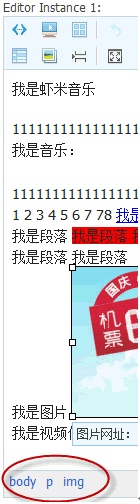
\includegraphics{elementpaths1.png}
\end{quote}


\subparagraph{sourcearea}
\label{relatedproj/editorguide/plugin:sourcearea}\begin{quote}

点击后可以查看编辑器产生的html代码.


\includegraphics{sourcearea1.png}
\end{quote}


\subparagraph{preview}
\label{relatedproj/editorguide/plugin:preview}\begin{quote}

点击后可以弹出新窗口, 查看编辑器的内容预览.


\includegraphics{preview1.png}
\end{quote}


\subparagraph{templates}
\label{relatedproj/editorguide/plugin:templates}\begin{quote}

点击后可以弹出模板选择窗口, 选定后可以将模板代码插入到编辑器光标所在处.


\includegraphics{templates1.png}
\end{quote}


\subparagraph{separator}
\label{relatedproj/editorguide/plugin:separator}\begin{quote}

间隔线.


\includegraphics{separator1.png}
\end{quote}


\subparagraph{undo}
\label{relatedproj/editorguide/plugin:undo}\begin{quote}

可以撤销重做.


\includegraphics{undo1.png}
\end{quote}


\subparagraph{removeformat}
\label{relatedproj/editorguide/plugin:removeformat}\begin{quote}

可以清除选择区域的编辑格式(字体, 大小, 加粗).


\includegraphics{removeformat1.png}
\end{quote}


\subparagraph{font}
\label{relatedproj/editorguide/plugin:font}\begin{quote}

大小: 可以改变选择区域字体的大小.

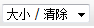
\includegraphics{fontsize1.png}

字体: 可以改变选择区域的字体种类.

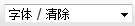
\includegraphics{fontfamily1.png}

粗体: 可以将选择区域文字加粗.


\includegraphics{fontbold1.png}

斜体: 可以将选择区域文字倾斜.


\includegraphics{fontitalic1.png}

下划线: 可以给选择区域文字加下划线.


\includegraphics{fontunderline1.png}

删除线: 可以给选择区域文字加删除线.


\includegraphics{fontdelete1.png}
\end{quote}


\subparagraph{format}
\label{relatedproj/editorguide/plugin:format}\begin{quote}

可以将光标所在处块加入标题格式.

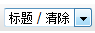
\includegraphics{format1.png}
\end{quote}


\subparagraph{color}
\label{relatedproj/editorguide/plugin:color}\begin{quote}

设置选择区域的文本颜色.


\includegraphics{forecolor1.png}

设置选择区域的背景颜色.


\includegraphics{bgcolor1.png}
\end{quote}


\subparagraph{list}
\label{relatedproj/editorguide/plugin:list}\begin{quote}

为选择区域或光标所在处加上项目编号.


\includegraphics{list11.png}

为选择区域或光标所在处加上列表编号.


\includegraphics{list21.png}
\end{quote}


\subparagraph{indent}
\label{relatedproj/editorguide/plugin:indent}\begin{quote}

减少光标处的缩进量.


\includegraphics{indent11.png}

增加光标处的缩进量.


\includegraphics{indent21.png}
\end{quote}


\subparagraph{justify}
\label{relatedproj/editorguide/plugin:justify}\begin{quote}

左对齐: 光标所在块左对齐.


\includegraphics{justify11.png}

居中对齐: 光标所在块居中对齐.


\includegraphics{justify21.png}

右对齐: 光标所在块右对齐.


\includegraphics{justify31.png}
\end{quote}


\subparagraph{link}
\label{relatedproj/editorguide/plugin:link}\begin{quote}

编辑选择区域的超链接.


\includegraphics{link1.png}
\end{quote}


\subparagraph{image}
\label{relatedproj/editorguide/plugin:image}\begin{quote}

输入图像地址将图像插入到光标所在处.


\includegraphics{image1.png}
\end{quote}


\subparagraph{flash}
\label{relatedproj/editorguide/plugin:flash}\begin{quote}

输入flash地址将flash插入到光标所在处.


\includegraphics{flash1.png}
\end{quote}


\subparagraph{music}
\label{relatedproj/editorguide/plugin:music}\begin{quote}

输入音乐地址将音乐插入到光标所在处.


\includegraphics{music1.png}
\end{quote}


\subparagraph{smiley}
\label{relatedproj/editorguide/plugin:smiley}\begin{quote}

选择表情并将对应表情插入到光标所在处.


\includegraphics{smiley1.png}
\end{quote}


\subparagraph{table}
\label{relatedproj/editorguide/plugin:table}\begin{quote}

输入表格相关参数并将对应表格插入到光标所在处.


\includegraphics{table1.png}
\end{quote}


\subparagraph{resize}
\label{relatedproj/editorguide/plugin:resize}\begin{quote}

可拖动调整编辑区域大小.

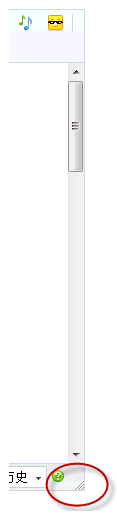
\includegraphics{resize1.png}
\end{quote}


\subparagraph{pagebreak}
\label{relatedproj/editorguide/plugin:pagebreak}\begin{quote}

插入分页标记.

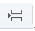
\includegraphics{pagebreak1.png}
\end{quote}


\subparagraph{maximize}
\label{relatedproj/editorguide/plugin:maximize}\begin{quote}

将编辑器充满整个屏幕.


\includegraphics{maximize1.png}
\end{quote}


\subparagraph{扩展插件}
\label{relatedproj/editorguide/plugin:id2}
如果要使用以下插件,需要引入另外的 javascript 文件

\begin{Verbatim}[commandchars=\\\{\}]
\PYG{n+nt}{\textless{}script }\PYG{n+na}{src=}\PYG{l+s}{"http://a.tbcdn.cn/s/kissy/1.1.7/editor/biz/ext/editor-plugin-pkg-min.js"}\PYG{n+nt}{\textgreater{}}\PYG{n+nt}{\textless{}/script\textgreater{}}
\end{Verbatim}


\subparagraph{multi-upload}
\label{relatedproj/editorguide/plugin:multi-upload}\begin{quote}

多图同时上传功能


\includegraphics{mul-upload1.png}

具体弹窗交互:

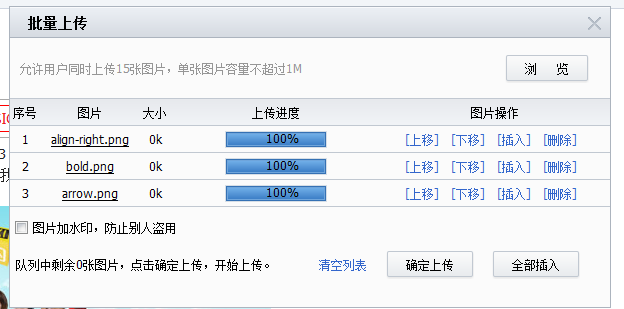
\includegraphics{mul-upload_win1.png}
\end{quote}


\subparagraph{checkbox-sourcearea}
\label{relatedproj/editorguide/plugin:checkbox-sourcearea}\begin{quote}

勾选交互的源码切换功能

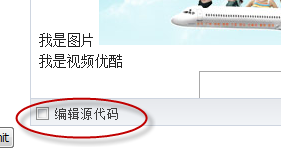
\includegraphics{checkbox-sourcearea1.png}
\end{quote}


\subparagraph{video}
\label{relatedproj/editorguide/plugin:video}\begin{quote}

国内视频插入,方便直接输入url插入国内视频 flash


\includegraphics{video1.png}

具体弹窗交互:

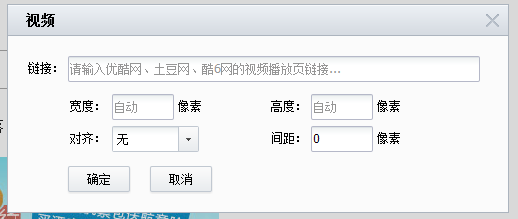
\includegraphics{video_win1.png}
\end{quote}


\subparagraph{xiami-music}
\label{relatedproj/editorguide/plugin:xiami-music}\begin{quote}

虾米音乐插入,可通过搜索插入虾米音乐


\includegraphics{xiami1.png}

具体弹窗交互:

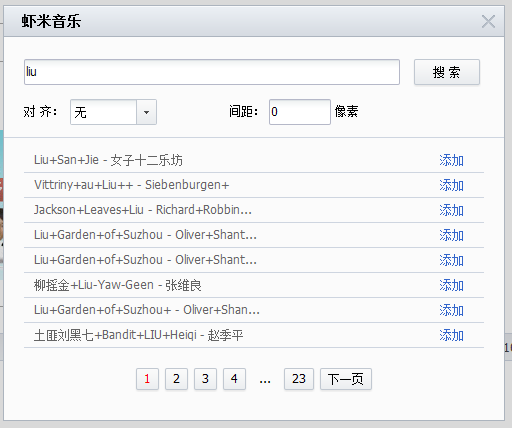
\includegraphics{xiami_win1.png}
\end{quote}


\paragraph{插件配置}
\label{relatedproj/editorguide/plugin-config::doc}\label{relatedproj/editorguide/plugin-config:editorusage-common-cfg}\label{relatedproj/editorguide/plugin-config:id1}


\begin{fulllineitems}
\pysigline{\bfcode{config.pluginConfig:}}{}
类型为各个插件的具体配置, 配置形式为:

\begin{Verbatim}[commandchars=@\[\]]
{
        "插件名":插件配置
}
\end{Verbatim}

包括以下插件配置:

\index{link (Editor.pluginConfig attribute)}

\begin{fulllineitems}
\phantomsection\label{relatedproj/editorguide/plugin-config:Editor.pluginConfig.link}\pysigline{\code{pluginConfig.}\bfcode{link}}{}
超链接配置,目前包括
\begin{quote}

\index{target (Editor.pluginConfig.link attribute)}

\begin{fulllineitems}
\phantomsection\label{relatedproj/editorguide/plugin-config:Editor.pluginConfig.link.target}\pysigline{\code{link.}\bfcode{target}}{}
默认为 ``'',表示在当前窗口打开新链接,也可以指定 ``\_blank'' ,则可以在新窗口打开链接。例如

\begin{Verbatim}[commandchars=\\\{\}]
\PYG{n+nx}{pluginConfig} \PYG{o}{:} \PYG{p}{\PYGZob{}}
    \PYG{n+nx}{link}\PYG{o}{:}\PYG{p}{\PYGZob{}}
        \PYG{n+nx}{target}\PYG{o}{:}\PYG{l+s+s2}{"\PYGZus{}blank"}
    \PYG{p}{\PYGZcb{}}
\PYG{p}{\PYGZcb{}}
\end{Verbatim}

\end{fulllineitems}

\end{quote}

\end{fulllineitems}


\index{upload (Editor.pluginConfig.image attribute)}

\begin{fulllineitems}
\phantomsection\label{relatedproj/editorguide/plugin-config:Editor.pluginConfig.image.upload}\pysigline{\code{pluginConfig.image.}\bfcode{upload}}{}
上传图片配置,不需要上传功能可不配置,包括以下子配置
\begin{quote}

\index{serverUrl (Editor.pluginConfig.image.upload attribute)}

\begin{fulllineitems}
\phantomsection\label{relatedproj/editorguide/plugin-config:Editor.pluginConfig.image.upload.serverUrl}\pysigline{\code{upload.}\bfcode{serverUrl}}{}
接受文件数据的服务器端程序地址,格式为 multipart/form-data ,返回格式为:
\begin{itemize}
\item {}
正确:\{``imgUrl'':''\href{http://xx.com/yy.jpg}{http://xx.com/yy.jpg}``\}

\item {}
错误:\{``error'':''i am error!''\}

\end{itemize}

\end{fulllineitems}


\index{serverParams (Editor.pluginConfig.image.upload attribute)}

\begin{fulllineitems}
\phantomsection\label{relatedproj/editorguide/plugin-config:Editor.pluginConfig.image.upload.serverParams}\pysigline{\code{upload.}\bfcode{serverParams}}{}
类型object,键值对。传给服务器的格外参数,如果 value 是函数则传递函数执行结果

\end{fulllineitems}


\index{suffix (Editor.pluginConfig.image.upload attribute)}

\begin{fulllineitems}
\phantomsection\label{relatedproj/editorguide/plugin-config:Editor.pluginConfig.image.upload.suffix}\pysigline{\code{upload.}\bfcode{suffix}}{}
类型字符串,允许图片的后缀名

\end{fulllineitems}


\index{fileInput (Editor.pluginConfig.image.upload attribute)}

\begin{fulllineitems}
\phantomsection\label{relatedproj/editorguide/plugin-config:Editor.pluginConfig.image.upload.fileInput}\pysigline{\code{upload.}\bfcode{fileInput}}{}
类型字符串,传给服务器的文件域名

\end{fulllineitems}


\index{sizeLimit (Editor.pluginConfig.image.upload attribute)}

\begin{fulllineitems}
\phantomsection\label{relatedproj/editorguide/plugin-config:Editor.pluginConfig.image.upload.sizeLimit}\pysigline{\code{upload.}\bfcode{sizeLimit}}{}
类型整数,限制上传的文件大小,单位 KB,ie 下只能作为提示。

\end{fulllineitems}


\index{extraHtml (Editor.pluginConfig.image.upload attribute)}

\begin{fulllineitems}
\phantomsection\label{relatedproj/editorguide/plugin-config:Editor.pluginConfig.image.upload.extraHtml}\pysigline{\code{upload.}\bfcode{extraHtml}}{}
放入图片上传区域的其他 html

\end{fulllineitems}

\end{quote}

例如:

\begin{Verbatim}[commandchars=\\\{\}]
\PYG{n+nx}{pluginConfig}\PYG{o}{:} \PYG{p}{\PYGZob{}}
    \PYG{c+c1}{// 图片插件配置}
    \PYG{l+s+s2}{"image"}\PYG{o}{:} \PYG{p}{\PYGZob{}}
        \PYG{c+c1}{//上传图片配置,不需要上传功能可不配置}
        \PYG{n+nx}{upload}\PYG{o}{:} \PYG{p}{\PYGZob{}}
            \PYG{c+c1}{//返回格式}
            \PYG{c+c1}{//正确:\PYGZob{}"imgUrl":"http://xx.com/yy.jpg"\PYGZcb{}}
            \PYG{c+c1}{//错误:\PYGZob{}"error":"i am error!"\PYGZcb{}}
            \PYG{c+c1}{//接受图片的服务器}
            \PYG{c+c1}{//发送一个文件过去,格式为 multipart/form-data}
            \PYG{n+nx}{serverUrl}\PYG{o}{:} \PYG{l+s+s2}{"/code/upload/upload.jsp"}\PYG{p}{,}
            \PYG{c+c1}{//传给服务器的格外参数,是函数则传递函数执行结果}
            \PYG{n+nx}{serverParams}\PYG{o}{:} \PYG{p}{\PYGZob{}}
                \PYG{n+nx}{yy}\PYG{o}{:} \PYG{k+kd}{function} \PYG{p}{(}\PYG{p}{)} \PYG{p}{\PYGZob{}}
                    \PYG{k}{return} \PYG{l+s+s2}{"xx"}\PYG{p}{;}
                \PYG{p}{\PYGZcb{}}
            \PYG{p}{\PYGZcb{}}\PYG{p}{,}
            \PYG{c+c1}{//后缀名白名单}
            \PYG{n+nx}{suffix}\PYG{o}{:} \PYG{l+s+s2}{"png,jpg,jpeg,gif"}\PYG{p}{,}
            \PYG{c+c1}{//传递给server的文件域名字}
            \PYG{n+nx}{fileInput}\PYG{o}{:} \PYG{l+s+s2}{"Filedata"}\PYG{p}{,}
            \PYG{c+c1}{//限制上传的文件大小,单位KB,}
            \PYG{c+c1}{//无法客户端限制,只能作为提示信息}
            \PYG{n+nx}{sizeLimit}\PYG{o}{:} \PYG{l+m+mi}{1000}\PYG{p}{,}
            \PYG{c+c1}{//k}
            \PYG{c+c1}{//自己想要添加的其他输入域}
            \PYG{n+nx}{extraHtml}\PYG{o}{:} \PYG{l+s+s2}{"\textless{}p style='margin-top:5px;'\textgreater{}"} \PYG{o}{+} \PYG{l+s+s2}{"\textless{}input type='checkbox' name='ke\PYGZus{}img\PYGZus{}up\PYGZus{}watermark\PYGZus{}1'\textgreater{} 图片加水印,防止别人盗用\textless{}/p\textgreater{}"}
        \PYG{p}{\PYGZcb{}}
    \PYG{p}{\PYGZcb{}}
\PYG{p}{\PYGZcb{}}
\end{Verbatim}

\begin{notice}{note}{Note:}
如果页面中设置了 document.domain='xx.com',那么这时上传图片服务器要返回一段设置 domain 的 html,例如

\begin{Verbatim}[commandchars=\\\{\}]
\PYG{n+nt}{\textless{}html}\PYG{n+nt}{\textgreater{}}
    \PYG{n+nt}{\textless{}head}\PYG{n+nt}{\textgreater{}}
        \PYG{n+nt}{\textless{}script}\PYG{n+nt}{\textgreater{}}
            \PYG{n+nb}{document}\PYG{p}{.}\PYG{n+nx}{domain}\PYG{o}{=}\PYG{l+s+s2}{"xx.com"}\PYG{p}{;}
        \PYG{n+nt}{\textless{}/script\textgreater{}}
    \PYG{n+nt}{\textless{}/head\textgreater{}}
    \PYG{n+nt}{\textless{}body}\PYG{n+nt}{\textgreater{}}
        \PYGZob{}"imgUrl":"http://img03.taobaocdn.com/sns\PYGZus{}album/i3/T13fhRXftcXXb1upjX.jpg"\PYGZcb{}
    \PYG{n+nt}{\textless{}/body\textgreater{}}
\PYG{n+nt}{\textless{}/html\textgreater{}}
\end{Verbatim}
\end{notice}

\end{fulllineitems}


\index{templates (Editor.pluginConfig attribute)}

\begin{fulllineitems}
\phantomsection\label{relatedproj/editorguide/plugin-config:Editor.pluginConfig.templates}\pysigline{\code{pluginConfig.}\bfcode{templates}}{}
模板 (templates) 配置,类型数组,数组每个元素为单个模板的配置,单个配置包括
\begin{quote}

\index{demo (Editor.pluginConfig.templates attribute)}

\begin{fulllineitems}
\phantomsection\label{relatedproj/editorguide/plugin-config:Editor.pluginConfig.templates.demo}\pysigline{\code{templates.}\bfcode{demo}}{}
类型字符串,模板的简单介绍

\end{fulllineitems}


\index{html (Editor.pluginConfig.templates attribute)}

\begin{fulllineitems}
\phantomsection\label{relatedproj/editorguide/plugin-config:Editor.pluginConfig.templates.html}\pysigline{\code{templates.}\bfcode{html}}{}
类型字符串,将要插入到编辑器区域的具体内容

\end{fulllineitems}

\end{quote}

例如:

\begin{Verbatim}[commandchars=\\\{\}]
\PYG{p}{\PYGZob{}}
    \PYG{l+s+s2}{"templates"}\PYG{o}{:} \PYG{p}{[}\PYG{p}{\PYGZob{}}
        \PYG{c+c1}{//显示模板的简单介绍}
        \PYG{n+nx}{demo}\PYG{o}{:} \PYG{l+s+s2}{"模板1效果演示html"}\PYG{p}{,}
        \PYG{c+c1}{//插入到编辑器区域的具体内容}
        \PYG{n+nx}{html}\PYG{o}{:} \PYG{l+s+s2}{"\textless{}div style='border:1px solid red'\textgreater{}模板1效果演示html\textless{}/div\textgreater{}\textless{}p\textgreater{}\textless{}/p\textgreater{}"}
    \PYG{p}{\PYGZcb{}}\PYG{p}{,}
    \PYG{p}{\PYGZob{}}
        \PYG{n+nx}{demo}\PYG{o}{:} \PYG{l+s+s2}{"模板2效果演示html"}\PYG{p}{,}
        \PYG{n+nx}{html}\PYG{o}{:} \PYG{l+s+s2}{"\textless{}div style='border:1px solid red'\textgreater{}模板2效果演示html\textless{}/div\textgreater{}"}
    \PYG{p}{\PYGZcb{}}\PYG{p}{]}\PYG{p}{,}
\PYG{p}{\PYGZcb{}}
\end{Verbatim}

\end{fulllineitems}




\begin{fulllineitems}
\pysigline{\bfcode{pluginConfig.font-size}}{}
字体大小配置,类型 object 或 boolean。当为 false 时,则该按钮不出现在编辑器中。当为 object 时,包含子配置
\begin{quote}



\begin{fulllineitems}
\pysigline{\bfcode{font-size.items}}{}
类型对象数组,数组每一项的配置为:
\begin{quote}

\index{value (Editor.items attribute)}

\begin{fulllineitems}
\phantomsection\label{relatedproj/editorguide/plugin-config:Editor.items.value}\pysigline{\code{items.}\bfcode{value}}{}
类型 string,真实的字体大小

\end{fulllineitems}


\index{attrs (Editor.items attribute)}

\begin{fulllineitems}
\phantomsection\label{relatedproj/editorguide/plugin-config:Editor.items.attrs}\pysigline{\code{items.}\bfcode{attrs}}{}
类型 object,键值对添加到每个字体的对应节点上

\end{fulllineitems}


\index{name (Editor.items attribute)}

\begin{fulllineitems}
\phantomsection\label{relatedproj/editorguide/plugin-config:Editor.items.name}\pysigline{\code{items.}\bfcode{name}}{}
类型 string,字体大小的显示值

\end{fulllineitems}

\end{quote}

\end{fulllineitems}

\end{quote}

例如:

\begin{Verbatim}[commandchars=\\\{\}]
\PYG{p}{\PYGZob{}}
    \PYG{l+s+s2}{"font-size"}\PYG{o}{:} \PYG{p}{\PYGZob{}}
        \PYG{c+c1}{//字体大小下拉框的配置}
        \PYG{n+nx}{items}\PYG{o}{:} \PYG{p}{[}\PYG{p}{\PYGZob{}}
            \PYG{c+c1}{//真实的字体大小值}
            \PYG{n+nx}{value}\PYG{o}{:} \PYG{l+s+s2}{"14px"}\PYG{p}{,}
            \PYG{c+c1}{//字体大小选项框样式,可不配置}
            \PYG{n+nx}{attrs}\PYG{o}{:} \PYG{p}{\PYGZob{}}
                \PYG{n+nx}{style}\PYG{o}{:} \PYG{l+s+s1}{'position: relative; border: 1px solid \#DDDDDD; margin: 2px; padding: 2px;'}
            \PYG{p}{\PYGZcb{}}\PYG{p}{,}
            \PYG{c+c1}{//单个字体大小的显示值}
            \PYG{n+nx}{name}\PYG{o}{:} \PYG{l+s+s2}{" \textless{}span style='font-size:14px'\textgreater{}标准\textless{}/span\textgreater{}"} \PYG{o}{+} \PYG{l+s+s2}{"\textless{}span style='position:absolute;top:1px;right:3px;'\textgreater{}14px\textless{}/span\textgreater{}"}
        \PYG{p}{\PYGZcb{}}\PYG{p}{]}
    \PYG{p}{\PYGZcb{}}

\PYG{p}{\PYGZcb{}}
\end{Verbatim}

\end{fulllineitems}




\begin{fulllineitems}
\pysigline{\bfcode{pluginConfig.font-family}}{}
字体种类配置,类型 object,包含子配置项
\begin{quote}



\begin{fulllineitems}
\pysigline{\bfcode{font-family.items}}{}
类型对象数组,字体种类配置,单个配置包含
\begin{quote}

\index{name (Editor.items attribute)}

\begin{fulllineitems}
\pysigline{\code{items.}\bfcode{name}}{}
字体显示值

\end{fulllineitems}


\index{value (Editor.items attribute)}

\begin{fulllineitems}
\pysigline{\code{items.}\bfcode{value}}{}
设置到编辑元素的真实值

\end{fulllineitems}

\end{quote}

\end{fulllineitems}

\end{quote}

例如:

\begin{Verbatim}[commandchars=\\\{\}]
\PYG{p}{\PYGZob{}}
    \PYG{l+s+s2}{"font-family"}\PYG{o}{:} \PYG{p}{\PYGZob{}}
        \PYG{n+nx}{items}\PYG{o}{:} \PYG{p}{[}\PYG{p}{\PYGZob{}}
            \PYG{c+c1}{//显示值}
            \PYG{n+nx}{name}\PYG{o}{:} \PYG{l+s+s2}{"宋体"}\PYG{p}{,}
            \PYG{c+c1}{//真实值}
            \PYG{n+nx}{value}\PYG{o}{:} \PYG{l+s+s2}{"SimSun"}
        \PYG{p}{\PYGZcb{}}\PYG{p}{,}
        \PYG{p}{\PYGZob{}}
            \PYG{n+nx}{name}\PYG{o}{:} \PYG{l+s+s2}{"黑体"}\PYG{p}{,}
            \PYG{n+nx}{value}\PYG{o}{:} \PYG{l+s+s2}{"SimHei"}
        \PYG{p}{\PYGZcb{}}\PYG{p}{]}
    \PYG{p}{\PYGZcb{}}
\PYG{p}{\PYGZcb{}}
\end{Verbatim}

\end{fulllineitems}




\begin{fulllineitems}
\pysigline{\bfcode{pluginConfig.font-bold}}{}
是否显示粗体按钮,默认 true

\end{fulllineitems}




\begin{fulllineitems}
\pysigline{\bfcode{pluginConfig.font-italic}}{}
是否显示斜体按钮,默认 true

\end{fulllineitems}




\begin{fulllineitems}
\pysigline{\bfcode{pluginConfig.font-underline}}{}
是否显示下划线按钮,默认 true

\end{fulllineitems}




\begin{fulllineitems}
\pysigline{\bfcode{pluginConfig.font-strikeThrough}}{}
是否显示删除线按钮,默认 true

\end{fulllineitems}


\index{draft (Editor.pluginConfig attribute)}

\begin{fulllineitems}
\phantomsection\label{relatedproj/editorguide/plugin-config:Editor.pluginConfig.draft}\pysigline{\code{pluginConfig.}\bfcode{draft}}{}
草稿箱

例如

\begin{Verbatim}[commandchars=\\\{\}]
\PYG{p}{\PYGZob{}}
    \PYG{l+s+s2}{"draft"}\PYG{o}{:} \PYG{p}{\PYGZob{}}
        \PYG{c+c1}{//分钟设置:每隔几分钟保存一次}
        \PYG{n+nx}{interval}\PYG{o}{:} \PYG{l+m+mi}{5}\PYG{p}{,}
        \PYG{c+c1}{//最多保存几条历史记录?}
        \PYG{n+nx}{limit}\PYG{o}{:} \PYG{l+m+mi}{10}\PYG{p}{,}
        \PYG{c+c1}{//草稿箱帮助文案,可不设置}
        \PYG{n+nx}{helpHtml}\PYG{o}{:} \PYG{l+s+s2}{"\textless{}div "} \PYG{o}{+} \PYG{l+s+s2}{"style='width:200px;'\textgreater{}"} \PYG{o}{+} \PYG{l+s+s2}{"\textless{}div style='padding:5px;'\textgreater{}草稿箱能够自动保存您最新编辑的内容,"} \PYG{o}{+} \PYG{l+s+s2}{"如果发现内容丢失,"} \PYG{o}{+} \PYG{l+s+s2}{"请选择恢复编辑历史\textless{}/div\textgreater{}\textless{}/div\textgreater{}"}
    \PYG{p}{\PYGZcb{}}
\PYG{p}{\PYGZcb{}}
\end{Verbatim}

\end{fulllineitems}


\index{resize (Editor.pluginConfig attribute)}

\begin{fulllineitems}
\phantomsection\label{relatedproj/editorguide/plugin-config:Editor.pluginConfig.resize}\pysigline{\code{pluginConfig.}\bfcode{resize}}{}
右下角调整大小的配置

例如

\begin{Verbatim}[commandchars=\\\{\}]
\PYG{p}{\PYGZob{}}
    \PYG{l+s+s2}{"resize"}\PYG{o}{:} \PYG{p}{\PYGZob{}}
        \PYG{c+c1}{//只能在y轴拖放,[“x”,”y”]表示任意拖放}
        \PYG{n+nx}{direction}\PYG{o}{:} \PYG{p}{[}\PYG{l+s+s2}{"y"}\PYG{p}{]}
    \PYG{p}{\PYGZcb{}}
\PYG{p}{\PYGZcb{}}
\end{Verbatim}

\end{fulllineitems}


\index{music (Editor.pluginConfig attribute)}

\begin{fulllineitems}
\phantomsection\label{relatedproj/editorguide/plugin-config:Editor.pluginConfig.music}\pysigline{\code{pluginConfig.}\bfcode{music}}{}
音乐插件配置,支持音乐文件地址输入,直接播放mp3

例如:

\begin{Verbatim}[commandchars=\\\{\}]
\PYG{n+nx}{music}\PYG{o}{:} \PYG{p}{\PYGZob{}}
    \PYG{c+c1}{//必须和网址url同域而不是类库同域}
    \PYG{n+nx}{musicPlayer}\PYG{o}{:} \PYG{l+s+s2}{"/music/niftyplayer.swf"}
\PYG{p}{\PYGZcb{}}
\end{Verbatim}

\end{fulllineitems}




\begin{fulllineitems}
\pysigline{\bfcode{pluginConfig.multi-upload}}{}
图片批量上传

例如

\begin{Verbatim}[commandchars=\\\{\}]
\PYG{p}{\PYGZob{}}
    \PYG{l+s+s2}{"multi-upload"}\PYG{o}{:} \PYG{p}{\PYGZob{}}
        \PYG{c+c1}{//同图片上传插件配置}
        \PYG{c+c1}{//返回格式}
        \PYG{c+c1}{//正确:\PYGZob{}"imgUrl":""\PYGZcb{}}
        \PYG{c+c1}{//错误:\PYGZob{}"error":""\PYGZcb{}}
        \PYG{c+c1}{//注意:中文 \PYGZbs{}uxxxx 转义}
        \PYG{c+c1}{//发送一个文件过去,格式为 multipart/form-data}
        \PYG{c+c1}{//接受图片的服务器,注意必须绝对地址}
        \PYG{n+nx}{serverUrl}\PYG{o}{:} \PYG{l+s+s2}{"http://xx.com/code/upload/upload.jsp"}\PYG{p}{,}
        \PYG{c+c1}{//同图片配置}
        \PYG{n+nx}{serverParams}\PYG{o}{:} \PYG{p}{\PYGZob{}}
            \PYG{n+nx}{waterMark}\PYG{o}{:} \PYG{k+kd}{function} \PYG{p}{(}\PYG{p}{)} \PYG{p}{\PYGZob{}}
                \PYG{k}{return} \PYG{n+nx}{S}\PYG{p}{.}\PYG{n+nx}{one}\PYG{p}{(}\PYG{l+s+s2}{"\#ke\PYGZus{}img\PYGZus{}up\PYGZus{}watermark\PYGZus{}2"}\PYG{p}{)}\PYG{p}{[}\PYG{l+m+mi}{0}\PYG{p}{]}\PYG{p}{.}\PYG{n+nx}{checked}\PYG{p}{;}
            \PYG{p}{\PYGZcb{}}
        \PYG{p}{\PYGZcb{}}\PYG{p}{,}
        \PYG{c+c1}{//同图片配置}
        \PYG{n+nx}{extraHtml}\PYG{o}{:} \PYG{l+s+s2}{"\textless{}p style='margin-top:10px;'\textgreater{}"} \PYG{o}{+} \PYG{l+s+s2}{"\textless{}input type='checkbox' "} \PYG{o}{+} \PYG{l+s+s2}{"style='vertical-align:middle;margin:0 5px;' "} \PYG{o}{+} \PYG{l+s+s2}{"id='ke\PYGZus{}img\PYGZus{}up\PYGZus{}watermark\PYGZus{}2'\textgreater{}"} \PYG{o}{+} \PYG{l+s+s2}{"\textless{}span style='vertical-align:middle;'\textgreater{}图片加水印,防止别人盗用\textless{}/span\textgreater{}\textless{}/p\textgreater{}"}\PYG{p}{,}
        \PYG{c+c1}{//缩略图的后缀名}
        \PYG{c+c1}{//原图:http://xx.com/yy.jpg}
        \PYG{c+c1}{//则加入后缀名时变为:}
        \PYG{c+c1}{//http://xx.com/yy\PYGZus{}80x80.jpg}
        \PYG{n+nx}{previewSuffix}\PYG{o}{:} \PYG{l+s+s2}{"\PYGZus{}80x80"}\PYG{p}{,}

        \PYG{c+c1}{//缩略图窗口宽度,高度根据图片自适应}
        \PYG{c+c1}{//若不需要缩略图功能,不配置即可}
        \PYG{n+nx}{previewWidth}\PYG{o}{:} \PYG{l+s+s2}{"80px"}\PYG{p}{,}

        \PYG{c+c1}{//客户端 flash 验证}
        \PYG{n+nx}{sizeLimit}\PYG{o}{:} \PYG{l+m+mi}{1000} \PYG{c+c1}{//k,}
        \PYG{c+c1}{//新增配置:可同时显示的图片列表个数}
        \PYG{n+nx}{numberLimit}\PYG{o}{:} \PYG{l+m+mi}{15}
    \PYG{p}{\PYGZcb{}}
\PYG{p}{\PYGZcb{}}
\end{Verbatim}

\begin{notice}{note}{Note:}
\#.该插件使用 flash 技术,必须在根域名下提供 crossdomain.xml ,例如 \href{http://www.taobao.com/crossdomain.xml}{http://www.taobao.com/crossdomain.xml} ,内容如下

\begin{Verbatim}[commandchars=\\\{\}]
\PYG{n+nt}{\textless{}cross-domain-policy}\PYG{n+nt}{\textgreater{}}
    \PYG{n+nt}{\textless{}allow-access-from} \PYG{n+na}{domain=}\PYG{l+s}{"*.taobao.com"}\PYG{n+nt}{/\textgreater{}}
    \PYG{n+nt}{\textless{}allow-access-from} \PYG{n+na}{domain=}\PYG{l+s}{"*.taobao.net"}\PYG{n+nt}{/\textgreater{}}
    \PYG{n+nt}{\textless{}allow-access-from} \PYG{n+na}{domain=}\PYG{l+s}{"*.taobaocdn.com"}\PYG{n+nt}{/\textgreater{}}
    \PYG{n+nt}{\textless{}allow-access-from} \PYG{n+na}{domain=}\PYG{l+s}{"*.tbcdn.cn"}\PYG{n+nt}{/\textgreater{}}
    \PYG{n+nt}{\textless{}allow-access-from} \PYG{n+na}{domain=}\PYG{l+s}{"*.allyes.com"}\PYG{n+nt}{/\textgreater{}}
\PYG{n+nt}{\textless{}/cross-domain-policy\textgreater{}}
\end{Verbatim}

\#.serverUrl 必须使用绝对地址,否则如果编辑器组件和应用页面不在同一个hostname时,firefox下请求会发到编辑器组件所在的hostname。
\end{notice}

\end{fulllineitems}


\index{video (Editor.pluginConfig attribute)}

\begin{fulllineitems}
\phantomsection\label{relatedproj/editorguide/plugin-config:Editor.pluginConfig.video}\pysigline{\code{pluginConfig.}\bfcode{video}}{}
国内视频插入,可直接输入tudou,youku,ku6的url进行视频粘贴.

例如:

\begin{Verbatim}[commandchars=\\\{\}]
\PYG{p}{\PYGZob{}}
    \PYG{l+s+s2}{"video"}\PYG{o}{:} \PYG{p}{\PYGZob{}}
        \PYG{n+nx}{urlCfg}\PYG{o}{:} \PYG{p}{[}\PYG{p}{\PYGZob{}}
            \PYG{n+nx}{reg}\PYG{o}{:} \PYG{l+s+sr}{/tudou\PYGZbs{}.com/i}\PYG{p}{,}
            \PYG{c+c1}{//地址配置后端咨询:石冲}
            \PYG{n+nx}{url}\PYG{o}{:} \PYG{l+s+s2}{"http://bangpai.daily.taobao.net/json/getTudouVideo.htm?"} \PYG{o}{+} \PYG{l+s+s2}{"url=@url@\&callback=@callback@"}
        \PYG{p}{\PYGZcb{}}\PYG{p}{]}\PYG{p}{,}
        \PYG{c+c1}{//输入框提示信息}
        \PYG{n+nx}{urlTip}\PYG{o}{:} \PYG{l+s+s2}{"请输入优酷网、土豆网、酷7网的视频播放页链接..."}\PYG{p}{,}
        \PYG{c+c1}{//静态转换规则,从用户输入转换为flash地址,例如优酷:}
        \PYG{n+nx}{providers}\PYG{o}{:} \PYG{p}{[}\PYG{p}{\PYGZob{}}
            \PYG{n+nx}{reg}\PYG{o}{:} \PYG{l+s+sr}{/youku\PYGZbs{}.com/i}\PYG{p}{,}
            \PYG{n+nx}{width}\PYG{o}{:} \PYG{l+m+mi}{480}\PYG{p}{,}
            \PYG{n+nx}{height}\PYG{o}{:} \PYG{l+m+mi}{400}\PYG{p}{,}
            \PYG{n+nx}{detect}\PYG{o}{:} \PYG{k+kd}{function} \PYG{p}{(}\PYG{n+nx}{url}\PYG{p}{)} \PYG{p}{\PYGZob{}}
                \PYG{k+kd}{var} \PYG{n+nx}{m} \PYG{o}{=} \PYG{n+nx}{url}\PYG{p}{.}\PYG{n+nx}{match}\PYG{p}{(}\PYG{l+s+sr}{/id\PYGZus{}([\PYGZca{}.]+)\PYGZbs{}.html\$/}\PYG{p}{)}\PYG{p}{;}
                \PYG{k}{if} \PYG{p}{(}\PYG{n+nx}{m}\PYG{p}{)} \PYG{p}{\PYGZob{}}
                    \PYG{k}{return} \PYG{l+s+s2}{"http://player.youku.com/player.php/sid/"} \PYG{o}{+} \PYG{n+nx}{m}\PYG{p}{[}\PYG{l+m+mi}{1}\PYG{p}{]} \PYG{o}{+} \PYG{l+s+s2}{"/v.swf"}\PYG{p}{;}
                \PYG{p}{\PYGZcb{}}
                \PYG{n+nx}{m} \PYG{o}{=} \PYG{n+nx}{url}\PYG{p}{.}\PYG{n+nx}{match}\PYG{p}{(}\PYG{l+s+sr}{/v\PYGZus{}playlist\PYGZbs{}/([\PYGZca{}.]+)\PYGZbs{}.html\$/}\PYG{p}{)}\PYG{p}{;}
                \PYG{k}{if} \PYG{p}{(}\PYG{n+nx}{m}\PYG{p}{)} \PYG{p}{\PYGZob{}}
                    \PYG{k}{return}\PYG{p}{;}
                    \PYG{c+c1}{//return "http://player.youku.com/player.php/sid/" + m[1] + "/v.swf";}
                \PYG{p}{\PYGZcb{}}
                \PYG{k}{return} \PYG{n+nx}{url}\PYG{p}{;}
            \PYG{p}{\PYGZcb{}}
        \PYG{p}{\PYGZcb{}}\PYG{p}{]}
    \PYG{p}{\PYGZcb{}}
\PYG{p}{\PYGZcb{}}
\end{Verbatim}

\end{fulllineitems}




\begin{fulllineitems}
\pysigline{\bfcode{pluginConfig.xiami-music}}{}
虾米音乐插入,无需配置, 只要 use 即可.

\end{fulllineitems}


\end{fulllineitems}


\begin{notice}{note}{Note:}
xiami-music , video , multi-upload 为扩展插件,若需要使用请引入外部js

\begin{Verbatim}[commandchars=\\\{\}]
\PYG{n+nt}{\textless{}script }\PYG{n+na}{src=}\PYG{l+s}{"http://a.tbcdn.cn/s/kissy/1.1.x/editor/biz/ext/editor-plugin-pkg-min.js"}\PYG{n+nt}{\textgreater{}}\PYG{n+nt}{\textless{}/script\textgreater{}}
\end{Verbatim}
\end{notice}


\subsubsection{注意}
\label{relatedproj/editorguide/notice:editorusage-notice}\label{relatedproj/editorguide/notice::doc}\label{relatedproj/editorguide/notice:id1}

\paragraph{应用样式}
\label{relatedproj/editorguide/notice:id2}
展示页面同样需要引入编辑器外部样式 :

\begin{Verbatim}[commandchars=\\\{\}]
\PYG{c}{\textless{}!--}\PYG{c}{[if lt IE 8]\textgreater{}}
\PYG{c}{\textless{}link href="http://a.tbcdn.cn/s/kissy/1.1.7/editor/theme/cool/editor}\PYG{c}{-}\PYG{c}{pkg}\PYG{c}{-}\PYG{c}{min}\PYG{c}{-}\PYG{c}{mhtml.css" rel="stylesheet"/\textgreater{}}
\PYG{c}{\textless{}![endif]}\PYG{c}{--\textgreater{}}
\PYG{c}{\textless{}!--}\PYG{c}{[if gte IE 8]\textgreater{}\textless{}!}\PYG{c}{--\textgreater{}}
\PYG{n+nt}{\textless{}link} \PYG{n+na}{href=}\PYG{l+s}{"http://a.tbcdn.cn/s/kissy/1.1.7/editor/theme/cool/editor-pkg-min-datauri.css"} \PYG{n+na}{rel=}\PYG{l+s}{"stylesheet"}\PYG{n+nt}{/\textgreater{}}
\PYG{c}{\textless{}!--}\PYG{c}{\textless{}![endif]}\PYG{c}{--\textgreater{}}
\end{Verbatim}

并且将从数据库中得到的编辑器生成内容用

\code{\textless{}div class="ke-post"\textgreater{}\textless{}/div\textgreater{}}

包裹起来.

如果使用了 {\hyperref[relatedproj/editorguide/plugin-config:editorusage-common-cfg]{\emph{一般配置中的自定义样式}}} ,
则需要在展示页面编辑器外部样式后重新定义你的自定义样式:

\begin{Verbatim}[commandchars=\\\{\}]
\PYG{n+nt}{\textless{}style }\PYG{n+na}{type=}\PYG{l+s}{"text/css"}\PYG{n+nt}{\textgreater{}}
    \PYG{n+nc}{.ke-post} \PYG{n+nt}{p} \PYG{p}{\PYGZob{}}
        \PYG{k}{color}\PYG{o}{:}\PYG{n+nb}{red}\PYG{p}{;}
    \PYG{p}{\PYGZcb{}}
\PYG{n+nt}{\textless{}/style\textgreater{}}
\end{Verbatim}


\paragraph{后端开发人员必看}
\label{relatedproj/editorguide/notice:id3}
\href{http://dev.taobao.net/?p=4033}{http://dev.taobao.net/?p=4033}


\subsubsection{FAQ}
\label{relatedproj/editorguide/faq:faq}\label{relatedproj/editorguide/faq::doc}

\paragraph{数据同步}
\label{relatedproj/editorguide/faq:id1}

\subparagraph{form 同步}
\label{relatedproj/editorguide/faq:form}\begin{quote}

如果后端通过 form 提交(submit)来获得用户输入数据,则只需配置参数 {\hyperref[relatedproj/editorguide/usage:Editor.KISSY.Editor]{\code{attachForm}}}  .

\begin{Verbatim}[commandchars=\\\{\}]
\PYG{c+c1}{//是否监控编辑器所属的表单提交}
\PYG{l+s+s2}{"attachForm"}\PYG{o}{:}\PYG{k+kc}{true}\PYG{p}{,}
\end{Verbatim}

编辑器自动会监控 form 的 sbumit 事件进行同步
\end{quote}


\subparagraph{手动同步}
\label{relatedproj/editorguide/faq:id2}\begin{quote}

涉及三个 api

editor 为调用 KISSY.Editor 返回的编辑器实例

\code{editor.sync()} : 手动同步编辑器内容到对应 textarea

\code{editor.getData()} : 获得当前编辑器的内容

\code{editor.setData(html:string)} :设置当前编辑器的内容,参数为html,类型为 string 字符串
\end{quote}


\paragraph{自动保存}
\label{relatedproj/editorguide/faq:id3}\begin{quote}

自动保存为 localStorage/flash 机制,保存在本地,可 {\hyperref[relatedproj/editorguide/plugin-config:Editor.pluginConfig.draft]{\code{配置参数}}} .
\end{quote}


\paragraph{字数统计}
\label{relatedproj/editorguide/faq:id4}\begin{quote}

可参考以下 demo  :

\href{http://docs.kissyui.com/kissy-editor/demo/cdn/1.1.7/wordCount.html}{http://docs.kissyui.com/kissy-editor/demo/cdn/1.1.7/wordCount.html}

其中 \href{http://docs.kissyui.com/kissy-editor/demo/word-count.js}{wordcount 代码} 自行下载,随意修改。
\end{quote}


\paragraph{绑定 ctrol-enter}
\label{relatedproj/editorguide/faq:ctrol-enter}
不少的应用场景要求在编辑器编辑区域内按下 ctrol+enter 按键时,编辑器所在表单会自动提交,解决方案是监控编辑器的文档按键事件:

\begin{Verbatim}[commandchars=\\\{\}]
\PYG{n+nx}{editor}\PYG{p}{.}\PYG{n+nx}{ready}\PYG{p}{(}\PYG{k+kd}{function} \PYG{p}{(}\PYG{p}{)} \PYG{p}{\PYGZob{}}
    \PYG{n+nx}{KISSY}\PYG{p}{.}\PYG{n+nx}{Event}\PYG{p}{.}\PYG{n+nx}{on}\PYG{p}{(}\PYG{n+nx}{editor}\PYG{p}{.}\PYG{n+nb}{document}\PYG{p}{,} \PYG{l+s+s2}{"keydown"}\PYG{p}{,} \PYG{k+kd}{function} \PYG{p}{(}\PYG{n+nx}{ev}\PYG{p}{)} \PYG{p}{\PYGZob{}}
        \PYG{k}{if} \PYG{p}{(}\PYG{n+nx}{ev}\PYG{p}{.}\PYG{n+nx}{keyCode} \PYG{o}{==} \PYG{l+m+mi}{13} \PYG{o}{\&\&} \PYG{n+nx}{ev}\PYG{p}{.}\PYG{n+nx}{ctrlKey}\PYG{p}{)} \PYG{p}{\PYGZob{}}
            \PYG{n+nx}{editor}\PYG{p}{.}\PYG{n+nx}{sync}\PYG{p}{(}\PYG{p}{)}\PYG{p}{;}
            \PYG{n+nx}{editor}\PYG{p}{.}\PYG{n+nx}{textarea}\PYG{p}{[}\PYG{l+m+mi}{0}\PYG{p}{]}\PYG{p}{.}\PYG{n+nx}{form}\PYG{p}{.}\PYG{n+nx}{submit}\PYG{p}{(}\PYG{p}{)}\PYG{p}{;}

        \PYG{p}{\PYGZcb{}}
    \PYG{p}{\PYGZcb{}}\PYG{p}{)}
\PYG{p}{\PYGZcb{}}\PYG{p}{)}\PYG{p}{;}
\end{Verbatim}

其中 editor 为编辑器实例的对象,通过 \code{var editor=KISSY.Editor("\#id",cfg)} 获取而来。


\paragraph{placeholder(tip) 功能}
\label{relatedproj/editorguide/faq:placeholder-tip}\begin{quote}

可参考以下 demo  :

\href{http://docs.kissyui.com/kissy-editor/demo/cdn/1.1.7/tip.html}{http://docs.kissyui.com/kissy-editor/demo/cdn/1.1.7/tip.html}

其中 \href{http://docs.kissyui.com/kissy-editor/demo/tip.js}{tip 代码} 自行下载,随意修改。
\end{quote}


\subsection{ppt}
\label{relatedproj/editorguide/index:ppt}\begin{quote}

\href{http://www.slideshare.net/yiminghe/kissy-editor}{kissy editor 开发与设计 @ webrebuild}
\end{quote}


\subsection{demo}
\label{relatedproj/editorguide/index:demo}\begin{quote}

\href{http://kissyteam.github.com/kissy-editor/demo/static-min-test.html}{http://kissyteam.github.com/kissy-editor/demo/static-min-test.html}
\end{quote}


\chapter{最佳编码实践}
\label{styleguide/index:styleguide}\label{styleguide/index::doc}\label{styleguide/index:id1}

\section{通用约定}
\label{styleguide/common-conventions:styleguide-commonconventions}\label{styleguide/common-conventions::doc}\label{styleguide/common-conventions:id1}

\subsection{文件与目录命名约定}
\label{styleguide/common-conventions:id2}\begin{enumerate}
\item {}
\textbf{一律小写,必须是英文单词或产品名称的拼音,多个单词用连字符(-)连接。} 只能出现英文字母、数字和连字符,严禁出现中文。

\item {}
出现版本号时,需要用字母 v 做为前缀,小版本号用点号(.)隔开,比如 global-v8.js 或 detail-v2.2.js 。

\item {}
该命名规范适用于 html, css, js, swf, php, xml, png, gif, jpg, ico 等前端维护的所有文件类型和相关目录。

\item {}
js 和 css 压缩文件,统一以 -min 结尾,比如源码文件为 kissy.js,压缩后为 kissy-min.js 。

\end{enumerate}


\subsection{文件编码约定}
\label{styleguide/common-conventions:id3}\begin{quote}

由于历史原因,前端开发涉及的所有文本文件请统一 \textbf{采用 GB2312, GBK 或 GB18030 编码} 。

注意:后台采用 UTF-8 的新项目,或自主开发的项目,推荐使用 UTF-8 编码。
\end{quote}


\subsection{id 和 class 命名约定}
\label{styleguide/common-conventions:id-class}\begin{enumerate}
\item {}
id 和 class 的命名总规则为: \textbf{内容优先,表现为辅} 。首先根据内容来命名,比如 main-nav. 如果根据内容找不到合适的命名,可以再结合表现来定,比如 skin-blue, present-tab, col-main.

\item {}
id 和 class 名称一律小写,多个单词用连字符连接,比如 recommend-presents.

\item {}
id 和 class 名称中只能出现小写的 26 个英文字母、数字和连字符(-),任何其它字符都严禁出现。

\item {}
id 和 class \textbf{尽量用英文单词命名} 。确实找不到合适的单词时,可以考虑使用产品的中文拼音,比如 wangwang, dating. 对于中国以及淘宝特色词汇,也可以使用拼音,比如 xiaobao, daigou. 除了产品名称和特色词汇,其它任何情况下都严禁使用拼音。

\item {}
在不影响语义的情况下,id 和 class 名称中可以适当采用英文单词缩写,比如 col, nav, hd, bd, ft 等,但切忌自造缩写。

\item {}
id 和 class 名称中的第一个词必须是单词全拼或语义非常清晰的单词缩写,比如 present, col.

\item {}
仅在 JavaScript 代码中当作 hook 用的 id 或 class, 命名规则为 J\_UpperCamelCase(请注意,J\_ 后的首字母也大写!), 其中字母 J 代表 JavaScript, 也是钩子(hook)的象形。注意:如果在 JavaScript 和 CSS 中都需要用到,则不用遵守本约定。

\item {}
在自动化测试脚本中当作 hook 用的 class, 命名规则为 T\_UpperCamelCase, 其中字母 T 代表 Test.

\end{enumerate}


\section{CSS 编码规范}
\label{styleguide/css-coding-style::doc}\label{styleguide/css-coding-style:styleguide-csscodingstyle}\label{styleguide/css-coding-style:css}\begin{itemize}
\item {}
待整理

\end{itemize}


\section{HTML 编码规范}
\label{styleguide/html-coding-style:styleguide-htmlcodingstyle}\label{styleguide/html-coding-style:html}\label{styleguide/html-coding-style::doc}

\subsection{基本规范}
\label{styleguide/html-coding-style:id1}\begin{itemize}
\item {}
使用符合语义的标签书写 HTML 文档,选择恰当的元素表达所需的含义;

\item {}
元素的标签和属性名必须小写,属性值必须加双引号;

\item {}
元素嵌套遵循 (X)HTML Strict 嵌套规则,推荐使用Firefox插件 \href{http://www.w3.org/TR/html4/}{HTML Validator} 进行检查;

\item {}
正确区分自闭合元素和非自闭合元素。非法闭合包括:\textless{}br\textgreater{}..\textless{}/br\textgreater{}、\textless{}script /\textgreater{}、\textless{}iframe /\textgreater{},非法闭合会导致页面嵌套错误问题;

\item {}
通过给元素设置自定义属性来存放与 JavaScript 交互的数据,属性名格式为 data-xx (例如:data-lazyload-url)

\end{itemize}


\subsection{文档模板}
\label{styleguide/html-coding-style:id2}
\begin{Verbatim}[commandchars=\\\{\}]
\PYG{c+cp}{\textless{}!doctype html\textgreater{}}
\PYG{n+nt}{\textless{}html}\PYG{n+nt}{\textgreater{}}
\PYG{n+nt}{\textless{}head}\PYG{n+nt}{\textgreater{}}
\PYG{n+nt}{\textless{}meta} \PYG{n+na}{charset=}\PYG{l+s}{"utf-8"} \PYG{n+nt}{/\textgreater{}}
\PYG{n+nt}{\textless{}title}\PYG{n+nt}{\textgreater{}}Sample page\PYG{n+nt}{\textless{}/title\textgreater{}}
\PYG{n+nt}{\textless{}link} \PYG{n+na}{rel=}\PYG{l+s}{"stylesheet"} \PYG{n+na}{href=}\PYG{l+s}{"css\PYGZus{}example\PYGZus{}url"} \PYG{n+nt}{/\textgreater{}}
\PYG{n+nt}{\textless{}script }\PYG{n+na}{src=}\PYG{l+s}{"js\PYGZus{}example\PYGZus{}url"}\PYG{n+nt}{\textgreater{}}\PYG{n+nt}{\textless{}/script\textgreater{}}
\PYG{n+nt}{\textless{}/head\textgreater{}}
\PYG{n+nt}{\textless{}body}\PYG{n+nt}{\textgreater{}}
\PYG{n+nt}{\textless{}div} \PYG{n+na}{id=}\PYG{l+s}{"page"}\PYG{n+nt}{\textgreater{}}
    \PYG{n+nt}{\textless{}div} \PYG{n+na}{id=}\PYG{l+s}{"header"}\PYG{n+nt}{\textgreater{}}
        页头
    \PYG{n+nt}{\textless{}/div\textgreater{}}
    \PYG{n+nt}{\textless{}div} \PYG{n+na}{id=}\PYG{l+s}{"content"}\PYG{n+nt}{\textgreater{}}
        主体
    \PYG{n+nt}{\textless{}/div\textgreater{}}
    \PYG{n+nt}{\textless{}div} \PYG{n+na}{id=}\PYG{l+s}{"footer"}\PYG{n+nt}{\textgreater{}}
        页尾
    \PYG{n+nt}{\textless{}/div\textgreater{}}
\PYG{n+nt}{\textless{}/div\textgreater{}}
\PYG{n+nt}{\textless{}script}\PYG{n+nt}{\textgreater{}}
\PYG{c+c1}{// 你的代码}
\PYG{n+nt}{\textless{}/script\textgreater{}}
\PYG{n+nt}{\textless{}/body\textgreater{}}
\PYG{n+nt}{\textless{}/html\textgreater{}}
\end{Verbatim}


\subsection{DOCTYPE}
\label{styleguide/html-coding-style:doctype}
页面文档类型统一使用HTML5 DOCTYPE。代码如下:

\begin{Verbatim}[commandchars=\\\{\}]
\PYG{c+cp}{\textless{}!doctype html\textgreater{}}
\end{Verbatim}


\subsection{编码}
\label{styleguide/html-coding-style:id3}
声明方法遵循HTML5的规范。

\begin{Verbatim}[commandchars=\\\{\}]
\PYG{n+nt}{\textless{}meta} \PYG{n+na}{charset=}\PYG{l+s}{"utf-8"} \PYG{n+nt}{/\textgreater{}}
\end{Verbatim}


\subsection{注释}
\label{styleguide/html-coding-style:id4}
建议对超过10行的页面模块进行注释,以降低开发人员的嵌套成本和后期的维护成本。例如:

\begin{Verbatim}[commandchars=\\\{\}]
\PYG{n+nt}{\textless{}div} \PYG{n+na}{id=}\PYG{l+s}{"sample"}\PYG{n+nt}{\textgreater{}}
    ...
\PYG{n+nt}{\textless{}/div\textgreater{}} \PYG{c}{\textless{}!--}\PYG{c}{ \#sample END }\PYG{c}{--\textgreater{}}
\end{Verbatim}

\begin{Verbatim}[commandchars=\\\{\}]
\PYG{n+nt}{\textless{}div} \PYG{n+na}{class=}\PYG{l+s}{"sample"}\PYG{n+nt}{\textgreater{}}
    ...
\PYG{n+nt}{\textless{}/div\textgreater{}} \PYG{c}{\textless{}!--}\PYG{c}{ .sample END }\PYG{c}{--\textgreater{}}
\end{Verbatim}


\subsection{元素}
\label{styleguide/html-coding-style:id5}

\subsubsection{结构性元素}
\label{styleguide/html-coding-style:id6}\begin{itemize}
\item {}
\code{p} 表示段落。只能包含内联元素,不能包含块级元素;

\item {}
\code{div} 本身无特殊含义,可用于布局。几乎可以包含任何元素;

\item {}
\code{br} 表示换行符;

\item {}
\code{hr} 表示水平分割线;

\item {}
\code{h1-h6} 表示标题。其中 h1 用于表示当前页面最重要的内容的标题;

\item {}
\code{blockquote} 表示引用,可以包含多个段落。请勿纯粹为了缩进而使用 blockquote,大部分浏览器默认将 blockquote 渲染为带有左右缩进;

\item {}
\code{pre} 表示一段格式化好的文本;

\end{itemize}


\subsubsection{头部元素}
\label{styleguide/html-coding-style:id7}\begin{itemize}
\item {}
\code{title} 每个页面必须有且仅有一个 title 元素;

\item {}
\code{base} 可用场景:首页、频道等大部分链接都为新窗口打开的页面;

\item {}
\code{link} link 用于引入 css 资源时,可省去 media(默认为all) 和 type(默认为text/css) 属性;

\item {}
\code{style} type 默认为 text/css,可以省去;

\item {}
\code{script} type 属性可以省去; 不赞成使用lang属性; 不要使用古老的\textless{}!– //–\textgreater{}这种hack脚本, 它用于阻止第一代浏览器(Netscape 1和Mosaic)将脚本显示成文字;

\item {}
\code{noscript} 在用户代理不支持 JavaScript 的情况下提供说明;

\end{itemize}


\subsubsection{文本元素}
\label{styleguide/html-coding-style:id8}\begin{itemize}
\item {}
\code{a} a 存在 href 属性时表示链接,无 href 属性但有 name 属性表示锚点;

\item {}
\code{em,strong} em 表示句意强调,加与不加会引起语义变化,可用于表示不同的心情或语调; strong 表示重要性强调,可用于局部或全局,strong强调的是重要性,不会改变句意;

\item {}
\code{abbr} 表示缩写;

\item {}
\code{sub,sup} 主要用于数学和化学公式,sup还可用于脚注;

\item {}
\code{span} 本身无特殊含义;

\item {}
\code{ins,del} 分别表示从文档中增加(插入)和删除

\end{itemize}


\subsubsection{媒体元素}
\label{styleguide/html-coding-style:id9}\begin{itemize}
\item {}
\code{img} 请勿将img元素作为定位布局的工具,不要用他显示空白图片; 必要时给img元素增加alt属性;

\item {}
\code{object} 可以用来插入Flash;

\end{itemize}


\subsubsection{列表元素}
\label{styleguide/html-coding-style:id10}\begin{itemize}
\item {}
\code{dl} 表示关联列表,dd是对dt的解释; dt和dd的对应关系比较随意:一个dt对应多个dd、多个dt对应一个dd、多个dt对应多个dd,都合法; 可用于名词/单词解释、日程列表、站点目录;

\item {}
\code{ul} 表示无序列表;

\item {}
\code{ol} 表示有序列表, 可用于排行榜等;

\item {}
\code{li} 表示列表项,必须是ul/ol的子元素;

\end{itemize}


\subsubsection{表单元素}
\label{styleguide/html-coding-style:id11}\begin{itemize}
\item {}
推荐使用 button 代替 input,但必须声明 type;

\item {}
推荐使用 fieldset,legend 组织表单

\item {}
表单元素的 name 不能设定为 action, enctype, method, novalidate, target, submit 会导致表单提交混乱

\end{itemize}


\subsection{参考文档}
\label{styleguide/html-coding-style:id12}\begin{itemize}
\item {}
\href{http://www.w3.org/TR/html4/}{http://www.w3.org/TR/html4/}

\item {}
\href{http://www.w3.org/TR/html5/}{http://www.w3.org/TR/html5/}

\item {}
\href{http://reference.sitepoint.com/html/}{http://reference.sitepoint.com/html/}

\end{itemize}


\section{JavaScript 语言规范}
\label{styleguide/js-lang-rules:styleguide-jslangrules}\label{styleguide/js-lang-rules:javascript}\label{styleguide/js-lang-rules::doc}\begin{itemize}
\item {}
声明变量时,必须加上 \code{var} 关键字。

\item {}
尽量减少全局变量的使用。

\item {}
语句总是以分号结尾。

\item {}
不要在块内声明函数。

\item {}
标准特性优于非标准特性(如果类库有提供,优先使用类库中的函数)。

\item {}
不要封装基本类型。

\item {}
只在解析序列化串时使用 \code{eval()} 。

\item {}
禁止使用 \code{with} 。

\item {}
减少使用 \code{continue} 和 \code{break} 。

\item {}
仅在函数内使用 \code{this} 。

\item {}
使用 \code{Array/Object} 直接量,避免使用 \code{Array/Object} 构造器。

\item {}
禁止修改内置对象的原型。

\end{itemize}


\section{JavaScript 编码风格}
\label{styleguide/js-style-rules:styleguide-jsstylerules}\label{styleguide/js-style-rules:javascript}\label{styleguide/js-style-rules::doc}

\subsection{行与缩进}
\label{styleguide/js-style-rules:id1}

\subsubsection{语句行}
\label{styleguide/js-style-rules:id2}\begin{enumerate}
\item {}
尽可能不要让每行超过 120 个字符;

\item {}
语句必须以分号作为结束符, 不要忽略分号;

\end{enumerate}


\subsubsection{空格}
\label{styleguide/js-style-rules:id3}\begin{enumerate}
\item {}
数值操作符(如, \code{+/-/*/\%} 等)两边留空;

\item {}
赋值操作符/等价判断符两边留一空格;

\item {}
for 循环条件中, 分号后留一空格;

\item {}
变量声明语句, 数组值, 对象值及函数参数值中的逗号后留一空格;

\item {}
空行不要有空格;

\item {}
行尾不要有空格;

\item {}
逗号和冒号后一定要跟空格;

\item {}
点号前后不要出现空格;

\item {}
空对象和数组不需要填入空格;

\item {}
函数名末尾和左括号之间不要出现空格;

\end{enumerate}


\subsubsection{空行}
\label{styleguide/js-style-rules:id4}\begin{enumerate}
\item {}
逻辑上独立的代码块使用空行分隔;

\item {}
文件末尾留 \code{1\textasciitilde{}2} 个空行;

\item {}
不要吝啬空行。尽量使用空行将逻辑相关的代码块分割开,以提高程序的可读性。

\end{enumerate}


\subsubsection{缩进}
\label{styleguide/js-style-rules:id5}\begin{enumerate}
\item {}
以 4 个空格为一缩进层次;

\item {}
变量声明:
\begin{itemize}
\item {}
多个变量声明时, 适当换行表示;

\item {}
参照 \code{var} 关键字, 缩进一层次;

\end{itemize}

\item {}
函数参数:
\begin{itemize}
\item {}
函数参数写在同一行上;

\item {}
传递匿名函数时, 函数体应从调用该函数的左边开始缩进;

\end{itemize}

\item {}
数组和对象初始化时:
\begin{itemize}
\item {}
如果初始值不是很长, 尽量保持写在单行上;

\item {}
初始值占用多行时, 缩进一层次;

\item {}
对象中, 比较长的变量/数值, 不要以冒号对齐;

\end{itemize}

\item {}
二元/三元操作符:
\begin{itemize}
\item {}
操作符始终跟随前行;

\item {}
实在需要缩进时, 按照上述缩进风格;

\end{itemize}

\item {}
表达式中的缩进同变量声明时;

\end{enumerate}


\subsection{括号}
\label{styleguide/js-style-rules:id6}
原则: 不要滥用括号, 必要时一定要使用.
\begin{enumerate}
\item {}
\code{if/else/while/for} 条件表达式必须有小括号;

\item {}
语句块必须有大括号;

\item {}
一元操作符(如 \code{delete, typeof, void})或在某些关键词(如 \code{return, throw, case, new}) 之后, 不要使用括号;

\end{enumerate}


\subsection{变量}
\label{styleguide/js-style-rules:id7}\begin{enumerate}
\item {}
变量如有较广的作用域, 使用全局变量; 如果是在类中, 可以设计成为一个类的成员;

\item {}
函数体中, 多个局部变量集中在一起声明, 避免分散;

\item {}
适当延迟变量的初始化;

\end{enumerate}


\subsection{字符串}
\label{styleguide/js-style-rules:id8}\begin{enumerate}
\item {}
JS 代码中, 单行字符串使用单引号;

\item {}
JS 代码中, 多行字符串使用 \code{+} 拼接形式, 不要使用 \code{\textbackslash{}} 拼接;

\item {}
HTML 中 \code{Element} 属性, 使用双引号;

\end{enumerate}


\subsection{命名规范}
\label{styleguide/js-style-rules:id9}
原则:
* 尽量避免潜在冲突;
* 精简短小, 见名知意;
\begin{enumerate}
\item {}
普通变量统一使用驼峰形式;

\item {}
常量使用全部大写, 多个单词以下划线分隔;

\item {}
枚举量, 同常量;

\item {}
私有变量, 属性和方法, 名字以下划线开头;

\item {}
保护变量, 属性和方法, 名字同普通变量名;

\item {}
方法和函数的可选参数, 名字以 \code{opt\_} 开头, 使用 \code{@param} 标记说明;

\item {} \begin{description}
\item[{方法和函数的参数个数不固定时:}] \leavevmode\begin{itemize}
\item {}
可添加参数 \code{var\_args} 为参数个数;

\item {}
取代使用 \code{arguments};

\item {}
使用 \code{@param} 标记说明;

\end{itemize}

\end{description}

\item {} \begin{description}
\item[{\code{Getter/Setter} 命名:}] \leavevmode\begin{itemize}
\item {}
以 \code{getFoo/setFoo(value)} 形式;

\item {}
布尔类型使用 \code{isFoo()/hasFoo()/canDo()/shouldDO()} 也可;

\end{itemize}

\end{description}

\item {} \begin{description}
\item[{命名空间:}] \leavevmode\begin{itemize}
\item {}
为全局代码使用命名空间, 如 \code{sloth.*};

\item {}
外部代码和内部代码使用不同的命名空间;

\end{itemize}

\end{description}

\item {}
重命名那些名字很长的变量, 不要在全局范围内创建别名, 而仅在函数块作用域中使用;

\item {}
文件名应全部使用小写字符, 且不包含除 \code{-} 和 \code{\_} 外的标点符号;

\item {}
临时的重复变量建议以 \code{i, j, k}, ..., 命名;

\end{enumerate}


\chapter{前端常用工具}
\label{tools/index:tools}\label{tools/index::doc}\label{tools/index:id1}\phantomsection\label{tools/module-compiler/index:module-module-compiler}
\index{module-compiler (module)}

\section{KISSY Module Compiler}
\label{tools/module-compiler/index:kissy-module-compiler}\label{tools/module-compiler/index::doc}
by \href{mailto:yiminghe@gmail.com}{承玉}


\subsection{简介}
\label{tools/module-compiler/intro::doc}\label{tools/module-compiler/intro:id1}\begin{itemize}
\item {}
是一个模块代码依赖自动合并工具。

\item {}
是一个模块代码规范辅助工具,可以辅助规范模块编写,不仅仅只适用动态加载场景,也可以用来提高开发阶段效率。

\item {}
是一个模块代码部署工具。结合 {\hyperref[api/seed/loader/index:module-Loader]{\code{KISSY 1.2 Loader}}} ,用于模块代码部署阶段,多个模块根据其依赖合并为一个文件,减少 HTTP 链接数。

\end{itemize}


\subsection{举例}
\label{tools/module-compiler/intro:id2}

\subsubsection{开发阶段}
\label{tools/module-compiler/intro:id3}
例如:现在有两个模块代码文件 \code{code/package/x.js} 与 \code{code/package/y.js}

\code{x.js} 中内容如下

\begin{Verbatim}[commandchars=\\\{\}]
\PYG{n+nx}{KISSY}\PYG{p}{.}\PYG{n+nx}{add}\PYG{p}{(}\PYG{k+kd}{function}\PYG{p}{(}\PYG{p}{)}\PYG{p}{\PYGZob{}}
    \PYG{k}{return} \PYG{l+s+s2}{"x"}\PYG{p}{;}
\PYG{p}{\PYGZcb{}}\PYG{p}{)}\PYG{p}{;}
\end{Verbatim}

\code{y.js} 中内容如下

\begin{Verbatim}[commandchars=\\\{\}]
\PYG{n+nx}{KISSY}\PYG{p}{.}\PYG{n+nx}{add}\PYG{p}{(}\PYG{k+kd}{function}\PYG{p}{(}\PYG{p}{)}\PYG{p}{\PYGZob{}}
    \PYG{k}{return} \PYG{l+s+s2}{"y"}\PYG{p}{;}
\PYG{p}{\PYGZcb{}}\PYG{p}{,}\PYG{p}{\PYGZob{}}\PYG{n+nx}{requires}\PYG{o}{:}\PYG{p}{[}\PYG{l+s+s2}{"./x"}\PYG{p}{]}\PYG{p}{\PYGZcb{}}\PYG{p}{)}\PYG{p}{;}
\end{Verbatim}

\code{x.js} 路径为 \code{http://x.cn/code/package/x.js} 开发阶段在页面中通过包配置 {\hyperref[api/seed/loader/add.ver1.2:Loader.KISSY.config]{\code{KISSY.config}}} 可以这样使用:

引入 KISSY

\begin{Verbatim}[commandchars=\\\{\}]
\PYG{n+nt}{\textless{}script }\PYG{n+na}{src=}\PYG{l+s}{'kissy.js'}\PYG{n+nt}{\textgreater{}}\PYG{n+nt}{\textless{}/script\textgreater{}}
\end{Verbatim}
\phantomsection\label{tools/module-compiler/intro:module-compiler-dev}
使用模块

\begin{Verbatim}[commandchars=\\\{\}]
\PYG{n+nx}{KISSY}\PYG{p}{.}\PYG{n+nx}{config}\PYG{p}{(}\PYG{p}{\PYGZob{}}
    \PYG{n+nx}{name}\PYG{o}{:}\PYG{l+s+s2}{"package"}\PYG{p}{,} \PYG{c+c1}{// 包名}
    \PYG{n+nx}{tag}\PYG{o}{:}\PYG{l+s+s2}{"20110323"}\PYG{p}{,} \PYG{c+c1}{// 动态加载包内的模块js文件时,}
                    \PYG{c+c1}{// 自动加上 ?t=20110323,用于文件更新}
    \PYG{n+nx}{path}\PYG{o}{:}\PYG{l+s+s2}{"http://x.cn/code/"}\PYG{p}{,} \PYG{c+c1}{// 包对应路径,相对路径指相对于当前页面路径}
    \PYG{n+nx}{charset}\PYG{o}{:}\PYG{l+s+s2}{"gbk"} \PYG{c+c1}{// 包里模块文件编码格式}
\PYG{p}{\PYGZcb{}}\PYG{p}{)}\PYG{p}{;}

\PYG{n+nx}{KISSY}\PYG{p}{.}\PYG{n+nx}{use}\PYG{p}{(}\PYG{l+s+s2}{"package/y"}\PYG{p}{,}\PYG{k+kd}{function}\PYG{p}{(}\PYG{n+nx}{S}\PYG{p}{,}\PYG{n+nx}{Y}\PYG{p}{)}\PYG{p}{\PYGZob{}}
    \PYG{c+c1}{// Y == "y"}
\PYG{p}{\PYGZcb{}}\PYG{p}{)}\PYG{p}{;}
\end{Verbatim}

那么 KISSY Loader 就会
\begin{enumerate}
\item {}
加载 \code{y.js} 。

\item {}
加载 \code{x.js} 。

\item {}
初始化 \code{package/x} 模块。

\item {}
初始化 \code{package/y} 模块。

\item {}
回调中可以得到 \code{package/x} 的模块值了。

\end{enumerate}

这个过程如果模块多的话对于线上环境来说 HTTP 链接数不可承受,使用 KISSY module compiler 则可以达到所有模块压缩为一个文件,达到 http 链接数为 1 的目标。


\subsubsection{使用 Module Compiler}
\label{tools/module-compiler/intro:module-compiler}
简要如下:
\begin{enumerate}
\item {}
配置 module compiler 指定需要的模块,这里即 \code{package/y}

\item {}
配置 module compiler 指定模块查找目录,这里即 \code{code/}

\item {}
配置 module compiler 指定合并后文件名称,假设为 \code{package/y.combine.js}

\item {}
运行 module compiler 合并 \code{package/y} 及其递归依赖的其他模块到 \code{package/y.combine.js}

\item {}
运行 closure compiler 压缩 \code{package/y.combine.js} 为 \code{package/y-min.js}

\end{enumerate}


\subsubsection{线上部署阶段}
\label{tools/module-compiler/intro:id4}
载入 \code{kissy} 的压缩版本

\begin{Verbatim}[commandchars=\\\{\}]
\PYG{n+nt}{\textless{}script }\PYG{n+na}{src=}\PYG{l+s}{'kissy-min.js'}\PYG{n+nt}{\textgreater{}}\PYG{n+nt}{\textless{}/script\textgreater{}}
\end{Verbatim}

使用模块部分同 {\hyperref[tools/module-compiler/intro:module-compiler-dev]{\emph{开发阶段}}} 。

线上过程:
\begin{enumerate}
\item {}
加载 \code{package/y-min.js}

\item {}
检查 \code{package/x} 模块,发现已经载入

\item {}
初始化 \code{package/x} 模块

\item {}
初始化 \code{package/y} 模块

\item {}
执行回调

\end{enumerate}

于是线上应用 HTTP 链接数为 1 。若需要使用源码调试则可以在页面 url 后加上 \code{?ks-debug} 即可开启开发阶段的加载过程.以上即为近期交易平台化项目所采用的模块化框架。


\subsection{使用说明}
\label{tools/module-compiler/usage::doc}\label{tools/module-compiler/usage:id1}
该工具为一个 jar 包,推荐嵌入到 ant 中,作为项目构建的一个阶段.

\begin{notice}{note}{Note:}
ant 以及相关压缩工具可直接使用 \href{https://github.com/kissyteam/kissy-tools}{kissy-tools} 中的文件,
建议直接下载整个 kissy-tools 作为项目工具一部分。
\end{notice}

使用前请先下载 kissy 源码到本地硬盘 \code{x:/kissy/} ,kissy-tools 源码到硬盘 \code{x:/kissy-tools/} ,假设项目源码在 \code{x:/code/} ,如上一节包括两个模块文件: \code{x:/code/package/x.js} 以及 \code{x:/code/package/y.js} ,则 ant 的调用为:

\begin{Verbatim}[commandchars=\\\{\}]
\PYG{n+nt}{\textless{}java} \PYG{n+na}{classname=}\PYG{l+s}{"com.taobao.f2e.Main"}\PYG{n+nt}{\textgreater{}}

    \PYG{n+nt}{\textless{}arg} \PYG{n+na}{value=}\PYG{l+s}{"-requires"}\PYG{n+nt}{/\textgreater{}}
    \PYG{n+nt}{\textless{}arg} \PYG{n+na}{value=}\PYG{l+s}{"package/y"}\PYG{n+nt}{/\textgreater{}}
    \PYG{n+nt}{\textless{}arg} \PYG{n+na}{value=}\PYG{l+s}{"-baseUrls"}\PYG{n+nt}{/\textgreater{}}
    \PYG{n+nt}{\textless{}arg} \PYG{n+na}{value=}\PYG{l+s}{"x:/kissy/,x:/code/"}\PYG{n+nt}{/\textgreater{}}
    \PYG{n+nt}{\textless{}arg} \PYG{n+na}{value=}\PYG{l+s}{"-encodings"}\PYG{n+nt}{/\textgreater{}}
    \PYG{n+nt}{\textless{}arg} \PYG{n+na}{value=}\PYG{l+s}{"utf-8,gbk"}\PYG{n+nt}{/\textgreater{}}
    \PYG{n+nt}{\textless{}arg} \PYG{n+na}{value=}\PYG{l+s}{"-outputEncoding"}\PYG{n+nt}{/\textgreater{}}
    \PYG{n+nt}{\textless{}arg} \PYG{n+na}{value=}\PYG{l+s}{"utf-8"}\PYG{n+nt}{/\textgreater{}}
    \PYG{n+nt}{\textless{}arg} \PYG{n+na}{value=}\PYG{l+s}{"-excludes"}\PYG{n+nt}{/\textgreater{}}
    \PYG{n+nt}{\textless{}arg} \PYG{n+na}{value=}\PYG{l+s}{"core"}\PYG{n+nt}{/\textgreater{}}
    \PYG{n+nt}{\textless{}arg} \PYG{n+na}{value=}\PYG{l+s}{"-output"}\PYG{n+nt}{/\textgreater{}}
    \PYG{n+nt}{\textless{}arg} \PYG{n+na}{value=}\PYG{l+s}{"x:/code/package/y.combine.js"}\PYG{n+nt}{/\textgreater{}}

    \PYG{n+nt}{\textless{}classpath}\PYG{n+nt}{\textgreater{}}
        \PYG{n+nt}{\textless{}pathelement} \PYG{n+na}{path=}\PYG{l+s}{"x:/kissy-tools/module-compiler/module-compiler.jar"}\PYG{n+nt}{/\textgreater{}}
        \PYG{n+nt}{\textless{}pathelement} \PYG{n+na}{path=}\PYG{l+s}{"\$\PYGZob{}java.class.path\PYGZcb{}"}\PYG{n+nt}{/\textgreater{}}
    \PYG{n+nt}{\textless{}/classpath\textgreater{}}

\PYG{n+nt}{\textless{}/java\textgreater{}}
\end{Verbatim}

如上所示该工具需要一些参数,包括 \code{requires}  , \code{baseUrls} , \code{encodings} , \code{outputEncoding} , \code{excludes} , \code{output} ,具体格式如下:


\subsubsection{requires}
\label{tools/module-compiler/usage:requires}
需要打包的模块名集合,该模块以及其递归依赖都会被一并打包。多个模块名用 \code{,} 分隔。如以上示例: \code{package/y} 。


\subsubsection{baseUrls}
\label{tools/module-compiler/usage:baseurls}
模块文件查找目录集合,一般存在两个: \code{kissy} 内置模块目录以及业务模块源码目录,目录间以 \code{,} 分隔。
如以上示例 \code{x:/kissy/,x:/code/} 。


\subsubsection{encodings}
\label{tools/module-compiler/usage:encodings}
指明模块目录中文件的编码,顺序对应于 \code{baseUrls} ,多个编码以 \code{,} 分隔。如以上示例: \code{utf-8,gbk} ,
表示 \code{kissy} 内置模块为 \code{utf-8} 编码,业务模块为 \code{gbk} 编码。


\subsubsection{outputEncoding}
\label{tools/module-compiler/usage:outputencoding}
指明最后合并打包文件的编码格式。如以上示例 \code{utf-8} 。


\subsubsection{excludes}
\label{tools/module-compiler/usage:excludes}
指明 \code{requires} 递归依赖模块中不需要打包的模块名称集合,该集合内的模块是单独动态加载或静态引入的,多个模块以 \code{,} 分隔。
如以上示例 \code{core} 表示 \code{kissy} 的 \code{core} 模块不需要合并打包,是通过 \code{kissy.js} 静态引入到页面中的。


\subsubsection{output}
\label{tools/module-compiler/usage:output}
指明最终合并打包后的文件路径以及名称。如以上示例: \code{x:/code/package/y.combine.js} ,
表示该工具产生的合并后文件为 \code{x:/code/package/y.combine.js} 。


\section{Sphinx 使用介绍}
\label{tools/use-sphinx:sphinx}\label{tools/use-sphinx::doc}\label{tools/use-sphinx:usesphinx}

\subsection{安装及使用 Sphinx}
\label{tools/use-sphinx:sphinx-install}\label{tools/use-sphinx:id1}
\textbf{解决依赖关系}
\begin{itemize}
\item {}
Python 2.x (\href{http://www.python.org/}{http://www.python.org/}), 并将 Python 加入到 Path 中;

\item {}
Setup Tools: Python 的一个包安装/管理工具(\href{http://pypi.python.org/pypi/setuptools}{http://pypi.python.org/pypi/setuptools}, win 下有 exe, 直接安装即可);

\item {}
安装 docutils, cmd 下进入 kissyteam/tools/docutils-0.7, 运行 python setup.py install;

\end{itemize}

\textbf{安装 Sphinx}
\begin{itemize}
\item {}
cmd 下运行: easy\_install -U Sphinx;

\item {}
cmd 下进入 kissyteam/tools/sphinx-to-github, 运行 python setup.py install;

\end{itemize}

\textbf{编译文档}
\begin{itemize}
\item {}
cmd 进入 kissyteam 目录, 运行 make.bat html , 在 docs 下生成 html;

\item {}
如果你想进一步了解如何创建 sphinx 工程, 见 \href{http://code.google.com/p/pymotwcn/wiki/SphinxprojectHowto}{http://code.google.com/p/pymotwcn/wiki/SphinxprojectHowto} ;

\end{itemize}


\subsection{reST 入门}
\label{tools/use-sphinx:rst-primer}\label{tools/use-sphinx:rest}
reST 是一种简单的标记语言, 规则非常简单.


\strong{See Also:}

\begin{itemize}
\item {}
完整的官方文档 \href{http://docutils.sourceforge.net/rst.html}{reStructuredText User Documentation}

\item {}
中文翻译版本: \href{http://wstudio.web.fc2.com/others/restructuredtext.html}{http://wstudio.web.fc2.com/others/restructuredtext.html}

\end{itemize}



\textbf{段落}

组织文档层次, 一般标题层次少于 4 级. 可以使用 :
\begin{itemize}
\item {}
\code{\#} 部分

\item {}
\code{*} 章节

\item {}
\code{=}, 大节

\item {}
\code{-}, 小节

\item {}
\code{\textasciicircum{}}, 小小节

\item {}
\code{"}, 段落

\end{itemize}

其实, 不同字符(\#, =, ` , {}`, \textasciicircum{}, * )没有等级区别, 只是你在使用时, 需要统一一种等级标记即可.

\textbf{行内标记}
\begin{itemize}
\item {}
一个星号表示斜体: \code{*text*}

\item {}
两个星号表示粗体: \code{**text**}

\item {}
两个反斜号表示行内代码: \code{{}`{}`text{}`{}`}

\end{itemize}

使用上的限制:
\begin{itemize}
\item {}
不能被嵌套,

\item {}
内容中不需要空白字符, 如: \code{* text*} , 这个是错误的写法,

\item {}
使用反斜杠进行转义: \code{thisis\textbackslash{} *one*\textbackslash{} word}

\end{itemize}

\textbf{无序/有序列表}

\begin{Verbatim}[commandchars=@\[\]]
* This is a bulleted list.
* It has two items, the second
  item uses two lines.

1. This is a numbered list.
2. It has two items too.

@#. This is a numbered list.
@#. It has two items too.
\end{Verbatim}

\textbf{嵌套列表}

\begin{Verbatim}[commandchars=@\[\]]
* this is
* a list

  * with a nested list
  * and some subitems

* and here the parent list continues
\end{Verbatim}

\textbf{定义列表}

\begin{Verbatim}[commandchars=@\[\]]
term (up to a line of text)
   Definition of the term, which must be indented

   and can even consist of multiple paragraphs

next term
   Description.
\end{Verbatim}

\textbf{注意} 以上, 只能是单行文字, 计算源码中有换行符, 但生成出来仍然以单行形式, 如果需要保留换行符, 可使用

\begin{Verbatim}[commandchars=@\[\]]
@textbar[] These lines are
@textbar[] broken exactly like in
@textbar[] the source file.
\end{Verbatim}

\textbf{嵌入源代码区块}

最普通的, 可以使用  \code{::} 标记, 表示接下来的缩进段落是表示一段代码,

\begin{Verbatim}[commandchars=@\[\]]
It is not processed in any way, except
that the indentation is removed.

It can span multiple lines.
\end{Verbatim}

需要高亮的源代码
\begin{itemize}
\item {}
嵌入 HTML 源代码

\begin{Verbatim}[commandchars=@\[\]]
.. raw:: html
   :file: inclusion.html

或者

.. raw:: html

    @textless[]a href="/kissy/docs/"@textgreater[]KISSY 文档@textless[]/a@textgreater[]
\end{Verbatim}

\item {}
嵌入 JS/CSS 等源代码, 及高亮显示( \href{http://pygments.org/}{http://pygments.org/} 上列出了支持的语言)

\begin{Verbatim}[commandchars=@\[\]]
.. code-block:: js

    alert('hi');
\end{Verbatim}

\end{itemize}

\textbf{表格}

生成这样的表格
\begin{quote}

\begin{tabulary}{\linewidth}{|L|L|L|}
\hline
\textbf{
A
} & \textbf{
B
} & \textbf{
A and B
}\\
\hline

False
 &
False
 &
False
\\

True
 &
False
 &
False
\\

False
 &
True
 &
False
\\

True
 &
True
 &
True
\\
\hline
\end{tabulary}

\end{quote}

使用的语法是

\begin{Verbatim}[commandchars=@\[\]]
=====  =====  =======
  A      B    A and B
=====  =====  =======
False  False  False
True   False  False
False  True   False
True   True   True
=====  =====  =======
\end{Verbatim}

\textbf{外部链接}

使用 \code{{}`链接  \textless{}http://example.com/\textgreater{}{}`\_} 表示外部链接, 也可以使用

\begin{Verbatim}[commandchars=@\[\]]
一段文字中包含 []`一个链接[]`@_.

.. @_另外一个链接: http://example.com/
\end{Verbatim}

\textbf{内部链接}
\begin{itemize}
\item {}
设定全局唯一的引用id, 如,  \code{.. \_my-reference-label:}

\item {}
在其他页面就可以使用这个id来引用, 如, \code{:ref:{}`提示文字 \textless{}my-reference-label\textgreater{}{}`}

\end{itemize}

例如

\begin{Verbatim}[commandchars=@\[\]]
.. @_my-reference-label:

Section to cross-reference
--------------------------

This is the text of the section.

It refers to the section itself, see :ref:[]`my-reference-label[]`.
\end{Verbatim}

\textbf{特殊标记}
\begin{itemize}
\item {}
\code{attention}, \code{caution}, \code{danger}, \code{error}, \code{hint}, \code{important}, \code{note}, \code{tip}, \code{warning}, \code{admonition} (最常用 ``note'' 和 ``warning''), 例如

\begin{Verbatim}[commandchars=@\[\]]
.. attention::

   Please attention
\end{Verbatim}

\end{itemize}

\begin{notice}{attention}{Attention:}
这是一个说明框.
\end{notice}

\begin{notice}{caution}{Caution:}
这是一个说明框.
\end{notice}

\begin{notice}{danger}{Danger:}
这是一个说明框.
\end{notice}

\begin{notice}{error}{Error:}
这是一个说明框.
\end{notice}

\begin{notice}{hint}{Hint:}
这是一个说明框.
\end{notice}

\begin{notice}{important}{Important:}
这是一个说明框.
\end{notice}

\begin{notice}{note}{Note:}
这是一个说明框.
\end{notice}

\begin{notice}{tip}{Tip:}
这是一个说明框.
\end{notice}

\begin{notice}{warning}{Warning:}
这是一个说明框.
\end{notice}

\begin{notice}{note}{自定义说明框}

这是一个说明框.
\end{notice}
\begin{itemize}
\item {}
插入图片

\begin{Verbatim}[commandchars=@\[\]]
.. image:: picture.jpeg
   :height: 100px
   :width: 200 px
   :scale: 50 @%
   :alt: alternate text
   :align: right
\end{Verbatim}

\end{itemize}

\textbf{注释}

单行

\begin{Verbatim}[commandchars=@\[\]]
.. 我是注释.
\end{Verbatim}

多行

\begin{Verbatim}[commandchars=@\[\]]
.. 我是注释
   我是注释
   我是注释
\end{Verbatim}

\textbf{脚注}

\begin{Verbatim}[commandchars=@\[\]]
Lorem ipsum @PYGZlb[]@#f1@PYGZrb[]@_ dolor sit amet ... @PYGZlb[]@#f2@PYGZrb[]@_

.. rubric:: Footnotes

.. @PYGZlb[]@#f1@PYGZrb[] Text of the first footnote.
.. @PYGZlb[]@#f2@PYGZrb[] Text of the second footnote.
\end{Verbatim}


\chapter{组件开发指南}
\label{workflow/index:id1}\label{workflow/index::doc}\label{workflow/index:workflow}

\section{KISSY 组件开发流程}
\label{workflow/workflow-simple:workflow-simple}\label{workflow/workflow-simple:kissy}\label{workflow/workflow-simple::doc}\begin{quote}

\begin{DUlineblock}{0em}
\item[] 欢迎加入KISSY开发小组!
\item[] 仅需几个简单的步骤,你就能跟更多人分享自己的代码,Let's Go!
\end{DUlineblock}
\end{quote}


\subsection{1、检出源码}
\label{workflow/workflow-simple:id1}\begin{quote}

\begin{DUlineblock}{0em}
\item[] 折腾派:请使用git拷贝“\href{https://github.com/kissyteam}{https://github.com/kissyteam}”的所有项目
\item[] 简单派:请使用svn检出“\href{http://svn.app.taobao.net/repos/fed/trunk/fed/kissy-team}{http://svn.app.taobao.net/repos/fed/trunk/fed/kissy-team}”目录(限淘宝)
\end{DUlineblock}
\end{quote}


\subsection{2、初始化工作文件夹}
\label{workflow/workflow-simple:id2}\begin{quote}

\begin{DUlineblock}{0em}
\item[] 想提供 \textbf{UI组件} 请进入“kissy-gallery”目录,解压“your-gallery.zip”文件
\item[] 想提供 \textbf{小功能} 请进入“kissy-util”目录,解压“your-util.zip”文件
\item[] 想提供 \textbf{设计模式} 请进入“kissy-dpl”目录,解压“your-dpl.zip”文件
\end{DUlineblock}

\begin{DUlineblock}{0em}
\item[] 这些文件夹都为你预置好了初始开发环境
\item[] 你只需要将其中的组件名改成你想写的即可快速开始工作
\item[] 并在文件中合适的地方为你提供了开发指引
\item[] 确保你能写出漂亮的代码
\end{DUlineblock}

\begin{DUlineblock}{0em}
\item[] 解压的文件夹都是带“.dev”后缀的
\item[] 这表示你的代码还在开发中
\item[] 开发完成后去掉即可
\end{DUlineblock}
\end{quote}


\subsection{3、编码}
\label{workflow/workflow-simple:id3}

\subsection{4、提交}
\label{workflow/workflow-simple:id4}
\begin{DUlineblock}{0em}
\item[] 怎么样,真的非常简单吧
\item[] 剩下的就交由KISSY管理团队处理,我们会在每周三同步两个仓库的修改,然后你的大作就能被大家欣赏了。
\item[] 当你需要写非常复杂的组件,或者希望重构以提高代码质量时,我们建议你参见 {\hyperref[workflow/workflow-full:workflow-full]{\emph{KISSY 组件开发流程(完整版)}}}.
\end{DUlineblock}


\section{KISSY 组件开发流程(完整版)}
\label{workflow/workflow-full:workflow-full}\label{workflow/workflow-full::doc}\label{workflow/workflow-full:kissy}
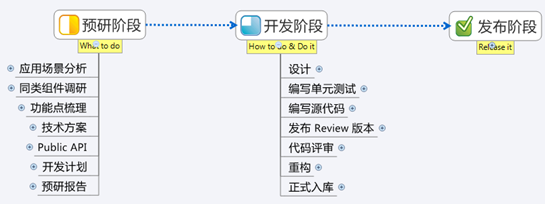
\includegraphics{workflow-s1.png}

点击查看详细大图


\subsection{步骤说明}
\label{workflow/workflow-full:id2}
请先阅读 \href{http://kissyteam.github.com/kissy/src/imagezoom/slide.html}{ImageZoom 调研文档}


\subsubsection{应用场景分析}
\label{workflow/workflow-full:id3}
一个需求到来, 比如这个图片放大效果, 首先我们需要这个功能能用在哪些地方, 或哪些网站上已经使用了, 如果有的话, 就对比一下不同的情况下不同的要求, 如 \#slide4 . 这样以后, 对比自己的需求, 想好要实现什么功能, 哪些功能保留, 哪些功能不需要, ---- 明确需求;


\subsubsection{同类组件调研}
\label{workflow/workflow-full:id4}
需求明确之后, 查找现有的同类组件, 看看他们针对这个问题, 是怎么实现的, 实现哪些功能, 哪些可以借鉴的地方, 哪些不足的地方要避免或者改进, 如 \#slide6 , ---- 明确要实现的功能有哪些;


\subsubsection{功能点梳理}
\label{workflow/workflow-full:id5}
分离出完成整个功能需要的几个核心功能点, 并针对各个功能点逐个描述, 如 \#slide8 , 这也可以帮你理清思路,  ---- 进一步明确待实现功能;


\subsubsection{技术方案}
\label{workflow/workflow-full:id6}
针对上述的几个功能点, 分别给出实现方案, 或者其他的技术难点, 又或者是算法上的分析等, 如 \#slide9 , --- 明确如何实现;


\subsubsection{Public API}
\label{workflow/workflow-full:public-api}
设计好的公共 API , 并在此说明, 也可以根据使用场景, 给出一些范例来说明 API 的使用, 如 \#slide14 , 这里可以在开始时设计的尽量精简些, ---- 明确 API 接口;


\subsubsection{开发计划}
\label{workflow/workflow-full:id7}
简略或者详细的制定一个开发计划, 及发布的版本和时间等, ---- 明确进度;


\subsubsection{预研报告}
\label{workflow/workflow-full:id8}
预研过程后总结一个报告, 可将报告分享给大家, 供大家一起讨论.

我们建议每个 KISSY 组件下, 都存放一个 slide.html, 其内容包含上述几部分内容. 这个 slide 随着你的开发过程的推进, 也会不断添加更新, 最后发布时连同组件源代码一起, 形成非常好的知识体系, 这样, 给别人或是几十年后的自己阅读, 也会像看文章一样的有条理.


\section{KISSY 组件开发规范}
\label{workflow/dev-spec:workflow-dev-spec}\label{workflow/dev-spec::doc}\label{workflow/dev-spec:kissy}
by \href{mailto:yiminghe@gmail.com}{承玉}

开始之前请先阅读 {\hyperref[workflow/workflow-simple:workflow-simple]{\emph{KISSY 组件开发流程}}}.


\subsection{确定 API}
\label{workflow/dev-spec:api}
首先确定该组件需要公开的 api 接口包括属性名称,函数名,参数以及返回值,可参考 YUI3 ,Jquery 等类库的同类组件,尽量保持一致。
比如 Overlay,那么其公开接口肯定包含方法 \code{show} ,{}`{}`hide{}`{}` 以及弹层内容 \code{content} 属性配置.


\subsection{模块编写}
\label{workflow/dev-spec:id2}
必须。推荐的目录结构如下,例如组件为 Overlay 弹层,那么该组件的目录结构应为:

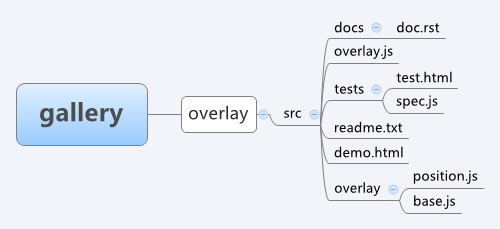
\includegraphics{component-guide1.png}

src 目录中必须包含和组件名相同的一个模块文件,模块名为 \code{gallery/overlay} ,用来指明该组件依赖的子模块,子模块的名约定为 \code{gallery/overlay/xx} ,如果组件比较简单也可只有这一个源码文件。例如 overlay.js

\begin{Verbatim}[commandchars=\\\{\}]
\PYG{n+nx}{KISSY}\PYG{p}{.}\PYG{n+nx}{add}\PYG{p}{(}\PYG{l+s+s2}{"gallery/overlay"}\PYG{p}{,}\PYG{k+kd}{function}\PYG{p}{(}\PYG{n+nx}{S}\PYG{p}{,}\PYG{n+nx}{Base}\PYG{p}{)}\PYG{p}{\PYGZob{}}
    \PYG{k}{return} \PYG{n+nx}{Base}\PYG{p}{;}
\PYG{p}{\PYGZcb{}}\PYG{p}{,}\PYG{p}{\PYGZob{}}
    \PYG{l+s+s1}{'./overlay/base'}\PYG{p}{,}\PYG{l+s+s1}{'./overlay/position'}
\PYG{p}{\PYGZcb{}}\PYG{p}{)}\PYG{p}{;}
\end{Verbatim}

子模块放在 \code{src} 模块名为目录名的文件夹内,对于 KISSY 1.2 以前,需要手动将组件挂载到 KISSY 上去并且需要在模块定义处挂载,例如子模块 base.js 的编写:

\begin{Verbatim}[commandchars=\\\{\}]
\PYG{n+nx}{KISSY}\PYG{p}{.}\PYG{n+nx}{add}\PYG{p}{(}\PYG{l+s+s2}{"gallery/overlay/base"}\PYG{p}{,}\PYG{k+kd}{function}\PYG{p}{(}\PYG{n+nx}{S}\PYG{p}{)}\PYG{p}{\PYGZob{}}
    \PYG{k+kd}{function} \PYG{n+nx}{Overlay}\PYG{p}{(}\PYG{p}{)}\PYG{p}{\PYGZob{}}\PYG{p}{\PYGZcb{}}

    \PYG{c+c1}{//如果需要兼容 KISSY \textless{} 1.2,需要手动挂载到 KISSY}
    \PYG{n+nx}{S}\PYG{p}{.}\PYG{n+nx}{namespace}\PYG{p}{(}\PYG{l+s+s2}{"Gallery"}\PYG{p}{)}\PYG{p}{;}
    \PYG{n+nx}{S}\PYG{p}{.}\PYG{n+nx}{Gallery}\PYG{p}{.}\PYG{n+nx}{Overlay}\PYG{o}{=}\PYG{n+nx}{Overlay}\PYG{p}{;}

    \PYG{k}{return} \PYG{n+nx}{Overlay}\PYG{p}{;}
\PYG{p}{\PYGZcb{}}\PYG{p}{)}\PYG{p}{;}
\end{Verbatim}

子模块间也可有依赖关系,例如子模块 position.js 需要对基本模块 base.js 进行增强 :

\begin{Verbatim}[commandchars=\\\{\}]
\PYG{n+nx}{KISSY}\PYG{p}{.}\PYG{n+nx}{add}\PYG{p}{(}\PYG{l+s+s2}{"gallery/overlay/position"}\PYG{p}{,}\PYG{k+kd}{function}\PYG{p}{(}\PYG{n+nx}{S}\PYG{p}{,}\PYG{n+nx}{Overlay}\PYG{p}{)}\PYG{p}{\PYGZob{}}
    \PYG{c+c1}{//兼容 kissy \textless{} 1.2}
    \PYG{n+nx}{Overlay} \PYG{o}{=} \PYG{n+nx}{S}\PYG{p}{.}\PYG{n+nx}{Gallery}\PYG{p}{.}\PYG{n+nx}{Overlay}\PYG{p}{;}

    \PYG{n+nx}{Overlay}\PYG{p}{.}\PYG{n+nx}{prototype}\PYG{p}{.}\PYG{n+nx}{xx}\PYG{o}{=}\PYG{k+kd}{function}\PYG{p}{(}\PYG{p}{)}\PYG{p}{\PYGZob{}}\PYG{p}{\PYGZcb{}}\PYG{p}{;}

\PYG{p}{\PYGZcb{}}\PYG{p}{,}\PYG{p}{\PYGZob{}}
    \PYG{n+nx}{requires}\PYG{o}{:}\PYG{p}{[}\PYG{l+s+s1}{'./base'}\PYG{p}{]}
\PYG{p}{\PYGZcb{}}\PYG{p}{)}\PYG{p}{;}
\end{Verbatim}


\subsection{demo 编写}
\label{workflow/dev-spec:demo}
必须。写一个 \code{demo.html} 简单展示下这个组件怎么用,静态载入组件的所有依赖js即可,注意被依赖模块js要放在依赖js前面,例如:

\begin{Verbatim}[commandchars=\\\{\}]
\PYG{c+cp}{\textless{}!DOCTYPE HTML\textgreater{}}
\PYG{n+nt}{\textless{}html}\PYG{n+nt}{\textgreater{}}
    \PYG{n+nt}{\textless{}head}\PYG{n+nt}{\textgreater{}}
        \PYG{n+nt}{\textless{}title}\PYG{n+nt}{\textgreater{}}overlay demo\PYG{n+nt}{\textless{}/title\textgreater{}}
    \PYG{n+nt}{\textless{}/head\textgreater{}}
    \PYG{n+nt}{\textless{}body}\PYG{n+nt}{\textgreater{}}
        \PYG{n+nt}{\textless{}script }\PYG{n+na}{src=}\PYG{l+s}{'../../../kissy/build/kissy.js'}\PYG{n+nt}{\textgreater{}}\PYG{n+nt}{\textless{}/script\textgreater{}}
        \PYG{n+nt}{\textless{}script }\PYG{n+na}{src=}\PYG{l+s}{'base.js'}\PYG{n+nt}{\textgreater{}}\PYG{n+nt}{\textless{}/script\textgreater{}}
        \PYG{n+nt}{\textless{}script }\PYG{n+na}{src=}\PYG{l+s}{'position.js'}\PYG{n+nt}{\textgreater{}}\PYG{n+nt}{\textless{}/script\textgreater{}}
        \PYG{n+nt}{\textless{}script }\PYG{n+na}{src=}\PYG{l+s}{'overlay.js'}\PYG{n+nt}{\textgreater{}}\PYG{n+nt}{\textless{}/script\textgreater{}}
        \PYG{n+nt}{\textless{}script}\PYG{n+nt}{\textgreater{}}
            \PYG{n+nx}{KISSY}\PYG{p}{.}\PYG{n+nx}{use}\PYG{p}{(}\PYG{l+s+s2}{"gallery/overlay"}\PYG{p}{,}\PYG{k+kd}{function}\PYG{p}{(}\PYG{n+nx}{S}\PYG{p}{,}\PYG{n+nx}{Overlay}\PYG{p}{)}\PYG{p}{\PYGZob{}}
                \PYG{c+c1}{// kissy \textless{} 1.2 获取}
                \PYG{n+nx}{Overlay}\PYG{o}{=}\PYG{n+nx}{S}\PYG{p}{.}\PYG{n+nx}{Gallery}\PYG{p}{.}\PYG{n+nx}{Overlay}\PYG{p}{;}
            \PYG{p}{\PYGZcb{}}\PYG{p}{)}\PYG{p}{;}
        \PYG{n+nt}{\textless{}/script\textgreater{}}
    \PYG{n+nt}{\textless{}/body\textgreater{}}
\PYG{n+nt}{\textless{}/html\textgreater{}}
\end{Verbatim}


\subsection{readme.txt 编写}
\label{workflow/dev-spec:readme-txt}

\subsection{文档编写}
\label{workflow/dev-spec:id3}
可选。在 \code{docs} 目录下编写组件文档,后缀名为 \code{rst} ,可参照 \code{KISSY Overlay} 的文档 \href{http://docs.kissyui.com/source/component/overlay/index.rst}{api}  以及
\href{http://docs.kissyui.com/source/component/overlay/usage.rst}{使用文档} ,详细格式可参见 \href{http://sphinx.pocoo.org/}{sphinx} 。文档不做强求,也可直接写纯文本格式,在 demo.html 详细讲解即可。


\subsection{单元测试编写}
\label{workflow/dev-spec:id6}
可选。在 \code{tests} 目录下编写单元测试代码,单元测试包括两个部分,测试准备页面以及单元测试用例脚本。


\subsubsection{测试准备页面}
\label{workflow/dev-spec:id7}
编写 test.html ,引入单元测试框架 jasmine (在 kissy/tools/ 下) ,例如:

\begin{Verbatim}[commandchars=\\\{\}]
\PYG{c+cp}{\textless{}!DOCTYPE html\textgreater{}}
\PYG{n+nt}{\textless{}html}\PYG{n+nt}{\textgreater{}}
    \PYG{n+nt}{\textless{}head}\PYG{n+nt}{\textgreater{}}
        \PYG{n+nt}{\textless{}meta} \PYG{n+na}{charset=}\PYG{l+s}{"utf-8"}\PYG{n+nt}{\textgreater{}}
        \PYG{n+nt}{\textless{}title}\PYG{n+nt}{\textgreater{}}Overlay Test Runner\PYG{n+nt}{\textless{}/title\textgreater{}}
        \PYG{n+nt}{\textless{}link} \PYG{n+na}{rel=}\PYG{l+s}{"stylesheet"} \PYG{n+na}{href=}\PYG{l+s}{"../../../tools/jasmine/jasmine.css"}\PYG{n+nt}{\textgreater{}}
        \PYG{n+nt}{\textless{}script }\PYG{n+na}{src=}\PYG{l+s}{"../../../kissy/tools/jasmine/jasmine.js"}\PYG{n+nt}{\textgreater{}}\PYG{n+nt}{\textless{}/script\textgreater{}}
        \PYG{n+nt}{\textless{}script }\PYG{n+na}{src=}\PYG{l+s}{"../../../kissy/tools/jasmine/jasmine-html.js"}\PYG{n+nt}{\textgreater{}}\PYG{n+nt}{\textless{}/script\textgreater{}}
        \PYG{n+nt}{\textless{}script }\PYG{n+na}{src=}\PYG{l+s}{"../../../kissy/tools/jasmine/event-simulate.js"}\PYG{n+nt}{\textgreater{}}\PYG{n+nt}{\textless{}/script\textgreater{}}
        \PYG{n+nt}{\textless{}script }\PYG{n+na}{src=}\PYG{l+s}{"../../../kissy/build/kissy.js"}\PYG{n+nt}{\textgreater{}}\PYG{n+nt}{\textless{}/script\textgreater{}}
    \PYG{n+nt}{\textless{}/head\textgreater{}}
    \PYG{n+nt}{\textless{}body}\PYG{n+nt}{\textgreater{}}
        \PYG{n+nt}{\textless{}script }\PYG{n+na}{src=}\PYG{l+s}{'base.js'}\PYG{n+nt}{\textgreater{}}\PYG{n+nt}{\textless{}/script\textgreater{}}
        \PYG{n+nt}{\textless{}script }\PYG{n+na}{src=}\PYG{l+s}{'position.js'}\PYG{n+nt}{\textgreater{}}\PYG{n+nt}{\textless{}/script\textgreater{}}
        \PYG{n+nt}{\textless{}script }\PYG{n+na}{src=}\PYG{l+s}{'overlay.js'}\PYG{n+nt}{\textgreater{}}\PYG{n+nt}{\textless{}/script\textgreater{}}
        \PYG{n+nt}{\textless{}script }\PYG{n+na}{src=}\PYG{l+s}{"overlay-spec.js"}\PYG{n+nt}{\textgreater{}}\PYG{n+nt}{\textless{}/script\textgreater{}}
        \PYG{n+nt}{\textless{}script}\PYG{n+nt}{\textgreater{}}
            \PYG{n+nx}{jasmine}\PYG{p}{.}\PYG{n+nx}{getEnv}\PYG{p}{(}\PYG{p}{)}\PYG{p}{.}\PYG{n+nx}{addReporter}\PYG{p}{(}\PYG{k}{new} \PYG{n+nx}{jasmine}\PYG{p}{.}\PYG{n+nx}{TrivialReporter}\PYG{p}{(}\PYG{p}{)}\PYG{p}{)}\PYG{p}{;}
            \PYG{n+nx}{jasmine}\PYG{p}{.}\PYG{n+nx}{getEnv}\PYG{p}{(}\PYG{p}{)}\PYG{p}{.}\PYG{n+nx}{execute}\PYG{p}{(}\PYG{k+kd}{function}\PYG{p}{(}\PYG{p}{)} \PYG{p}{\PYGZob{}}
                \PYG{k}{if} \PYG{p}{(}\PYG{n+nx}{parent} \PYG{o}{\&\&} \PYG{n+nx}{parent}\PYG{p}{.}\PYG{n+nx}{jasmine}\PYG{p}{.}\PYG{n+nx}{kissyNext}\PYG{p}{)} \PYG{p}{\PYGZob{}}
                    \PYG{n+nx}{parent}\PYG{p}{.}\PYG{n+nx}{jasmine}\PYG{p}{.}\PYG{n+nx}{kissyNext}\PYG{p}{(}\PYG{k}{this}\PYG{p}{.}\PYG{n+nx}{results}\PYG{p}{(}\PYG{p}{)}\PYG{p}{.}\PYG{n+nx}{failedCount}\PYG{p}{)}\PYG{p}{;}
                \PYG{p}{\PYGZcb{}}
            \PYG{p}{\PYGZcb{}}\PYG{p}{)}\PYG{p}{;}
        \PYG{n+nt}{\textless{}/script\textgreater{}}
    \PYG{n+nt}{\textless{}/body\textgreater{}}
\PYG{n+nt}{\textless{}/html\textgreater{}}
\end{Verbatim}


\subsubsection{测试用例脚本编写}
\label{workflow/dev-spec:id8}
测试用例编写在脚本 \code{overlay-spec.js} 中,详细可参考 \href{https://github.com/pivotal/jasmine/wiki}{jasmine wiki} ,这里简单举个例子:

\begin{Verbatim}[commandchars=\\\{\}]
\PYG{c+c1}{// 测试用例脚本可以包含很多 suit}
\PYG{n+nx}{describe}\PYG{p}{(}\PYG{l+s+s2}{"开始一个 suit"}\PYG{p}{,}\PYG{k+kd}{function}\PYG{p}{(}\PYG{p}{)}\PYG{p}{\PYGZob{}}

    \PYG{c+c1}{// 一个 suit 包含很多 spec}
    \PYG{n+nx}{it}\PYG{p}{(}\PYG{l+s+s2}{"开始一个 spec"}\PYG{p}{,}\PYG{k+kd}{function}\PYG{p}{(}\PYG{p}{)}\PYG{p}{\PYGZob{}}

        \PYG{c+cm}{/*}
\PYG{c+cm}{            一个 spec 包含很多 expectation}
\PYG{c+cm}{        */}
        \PYG{n+nx}{expect}\PYG{p}{(}\PYG{l+s+s2}{"xx"}\PYG{p}{)}\PYG{p}{.}\PYG{n+nx}{toBe}\PYG{p}{(}\PYG{l+s+s2}{"xx"}\PYG{p}{)}\PYG{p}{;}
        \PYG{n+nx}{expect}\PYG{p}{(}\PYG{l+s+s2}{"yy"}\PYG{p}{)}\PYG{p}{.}\PYG{n+nx}{toBe}\PYG{p}{(}\PYG{l+s+s2}{"yy"}\PYG{p}{)}\PYG{p}{;}

    \PYG{p}{\PYGZcb{}}\PYG{p}{)}\PYG{p}{;}

\PYG{p}{\PYGZcb{}}\PYG{p}{)}\PYG{p}{;}
\end{Verbatim}

复杂点的例子可以看 \href{https://github.com/kissyteam/kissy/blob/master/src/overlay/tests/overlay-spec.js}{KISSY.Overlay Unit Test}


\renewcommand{\indexname}{Python Module Index}
\begin{theindex}
\def\bigletter#1{{\Large\sffamily#1}\nopagebreak\vspace{1mm}}
\bigletter{d}
\item {\texttt{DataLazyload}}, \pageref{demo/component/datalazyload/index:module-DataLazyload}
\item {\texttt{DD}}, \pageref{api/component/dd/index:module-DD}
\item {\texttt{DOM}}, \pageref{api/core/dom/index:module-DOM}
\indexspace
\bigletter{e}
\item {\texttt{Editor}}, \pageref{relatedproj/editorguide/index:module-Editor}
\indexspace
\bigletter{l}
\item {\texttt{Lang}}, \pageref{api/seed/lang/index:module-Lang}
\item {\texttt{Loader}}, \pageref{api/seed/loader/index:module-Loader}
\indexspace
\bigletter{m}
\item {\texttt{module-compiler}}, \pageref{tools/module-compiler/index:module-module-compiler}
\indexspace
\bigletter{n}
\item {\texttt{Node}}, \pageref{api/core/node/index:module-Node}
\indexspace
\bigletter{o}
\item {\texttt{Overlay}}, \pageref{api/component/overlay/index:module-Overlay}
\indexspace
\bigletter{s}
\item {\texttt{Seed}}, \pageref{api/seed/kissy/index:module-Seed}
\item {\texttt{Suggest}}, \pageref{api/component/suggest/index:module-Suggest}
\item {\texttt{Switchable}}, \pageref{api/component/switchable/index:module-Switchable}
\indexspace
\bigletter{t}
\item {\texttt{Template}}, \pageref{api/component/template/index:module-Template}
\indexspace
\bigletter{w}
\item {\texttt{Web}}, \pageref{api/seed/web/index:module-Web}
\end{theindex}

\renewcommand{\indexname}{Index}
\printindex
\end{document}
